% Options for packages loaded elsewhere
% Options for packages loaded elsewhere
\PassOptionsToPackage{unicode}{hyperref}
\PassOptionsToPackage{hyphens}{url}
%
\documentclass[
  11pt,
  letterpaper,
]{book}
\usepackage{xcolor}
\usepackage[margin=2.5cm,paper=a4paper]{geometry}
\usepackage{amsmath,amssymb}
\setcounter{secnumdepth}{5}
\usepackage{iftex}
\ifPDFTeX
  \usepackage[T1]{fontenc}
  \usepackage[utf8]{inputenc}
  \usepackage{textcomp} % provide euro and other symbols
\else % if luatex or xetex
  \usepackage{unicode-math} % this also loads fontspec
  \defaultfontfeatures{Scale=MatchLowercase}
  \defaultfontfeatures[\rmfamily]{Ligatures=TeX,Scale=1}
\fi
\usepackage{lmodern}
\ifPDFTeX\else
  % xetex/luatex font selection
\fi
% Use upquote if available, for straight quotes in verbatim environments
\IfFileExists{upquote.sty}{\usepackage{upquote}}{}
\IfFileExists{microtype.sty}{% use microtype if available
  \usepackage[]{microtype}
  \UseMicrotypeSet[protrusion]{basicmath} % disable protrusion for tt fonts
}{}
\makeatletter
\@ifundefined{KOMAClassName}{% if non-KOMA class
  \IfFileExists{parskip.sty}{%
    \usepackage{parskip}
  }{% else
    \setlength{\parindent}{0pt}
    \setlength{\parskip}{6pt plus 2pt minus 1pt}}
}{% if KOMA class
  \KOMAoptions{parskip=half}}
\makeatother
% Make \paragraph and \subparagraph free-standing
\makeatletter
\ifx\paragraph\undefined\else
  \let\oldparagraph\paragraph
  \renewcommand{\paragraph}{
    \@ifstar
      \xxxParagraphStar
      \xxxParagraphNoStar
  }
  \newcommand{\xxxParagraphStar}[1]{\oldparagraph*{#1}\mbox{}}
  \newcommand{\xxxParagraphNoStar}[1]{\oldparagraph{#1}\mbox{}}
\fi
\ifx\subparagraph\undefined\else
  \let\oldsubparagraph\subparagraph
  \renewcommand{\subparagraph}{
    \@ifstar
      \xxxSubParagraphStar
      \xxxSubParagraphNoStar
  }
  \newcommand{\xxxSubParagraphStar}[1]{\oldsubparagraph*{#1}\mbox{}}
  \newcommand{\xxxSubParagraphNoStar}[1]{\oldsubparagraph{#1}\mbox{}}
\fi
\makeatother
\usepackage{fancyvrb}

\usepackage{color}
\usepackage{fancyvrb}
\newcommand{\VerbBar}{|}
\newcommand{\VERB}{\Verb[commandchars=\\\{\}]}
\DefineVerbatimEnvironment{Highlighting}{Verbatim}{commandchars=\\\{\}}
% Add ',fontsize=\small' for more characters per line
\usepackage{framed}
\definecolor{shadecolor}{RGB}{241,243,245}
\newenvironment{Shaded}{\begin{snugshade}}{\end{snugshade}}
\newcommand{\AlertTok}[1]{\textcolor[rgb]{0.68,0.00,0.00}{#1}}
\newcommand{\AnnotationTok}[1]{\textcolor[rgb]{0.37,0.37,0.37}{#1}}
\newcommand{\AttributeTok}[1]{\textcolor[rgb]{0.40,0.45,0.13}{#1}}
\newcommand{\BaseNTok}[1]{\textcolor[rgb]{0.68,0.00,0.00}{#1}}
\newcommand{\BuiltInTok}[1]{\textcolor[rgb]{0.00,0.23,0.31}{#1}}
\newcommand{\CharTok}[1]{\textcolor[rgb]{0.13,0.47,0.30}{#1}}
\newcommand{\CommentTok}[1]{\textcolor[rgb]{0.37,0.37,0.37}{#1}}
\newcommand{\CommentVarTok}[1]{\textcolor[rgb]{0.37,0.37,0.37}{\textit{#1}}}
\newcommand{\ConstantTok}[1]{\textcolor[rgb]{0.56,0.35,0.01}{#1}}
\newcommand{\ControlFlowTok}[1]{\textcolor[rgb]{0.00,0.23,0.31}{\textbf{#1}}}
\newcommand{\DataTypeTok}[1]{\textcolor[rgb]{0.68,0.00,0.00}{#1}}
\newcommand{\DecValTok}[1]{\textcolor[rgb]{0.68,0.00,0.00}{#1}}
\newcommand{\DocumentationTok}[1]{\textcolor[rgb]{0.37,0.37,0.37}{\textit{#1}}}
\newcommand{\ErrorTok}[1]{\textcolor[rgb]{0.68,0.00,0.00}{#1}}
\newcommand{\ExtensionTok}[1]{\textcolor[rgb]{0.00,0.23,0.31}{#1}}
\newcommand{\FloatTok}[1]{\textcolor[rgb]{0.68,0.00,0.00}{#1}}
\newcommand{\FunctionTok}[1]{\textcolor[rgb]{0.28,0.35,0.67}{#1}}
\newcommand{\ImportTok}[1]{\textcolor[rgb]{0.00,0.46,0.62}{#1}}
\newcommand{\InformationTok}[1]{\textcolor[rgb]{0.37,0.37,0.37}{#1}}
\newcommand{\KeywordTok}[1]{\textcolor[rgb]{0.00,0.23,0.31}{\textbf{#1}}}
\newcommand{\NormalTok}[1]{\textcolor[rgb]{0.00,0.23,0.31}{#1}}
\newcommand{\OperatorTok}[1]{\textcolor[rgb]{0.37,0.37,0.37}{#1}}
\newcommand{\OtherTok}[1]{\textcolor[rgb]{0.00,0.23,0.31}{#1}}
\newcommand{\PreprocessorTok}[1]{\textcolor[rgb]{0.68,0.00,0.00}{#1}}
\newcommand{\RegionMarkerTok}[1]{\textcolor[rgb]{0.00,0.23,0.31}{#1}}
\newcommand{\SpecialCharTok}[1]{\textcolor[rgb]{0.37,0.37,0.37}{#1}}
\newcommand{\SpecialStringTok}[1]{\textcolor[rgb]{0.13,0.47,0.30}{#1}}
\newcommand{\StringTok}[1]{\textcolor[rgb]{0.13,0.47,0.30}{#1}}
\newcommand{\VariableTok}[1]{\textcolor[rgb]{0.07,0.07,0.07}{#1}}
\newcommand{\VerbatimStringTok}[1]{\textcolor[rgb]{0.13,0.47,0.30}{#1}}
\newcommand{\WarningTok}[1]{\textcolor[rgb]{0.37,0.37,0.37}{\textit{#1}}}

\usepackage{longtable,booktabs,array}
\usepackage{calc} % for calculating minipage widths
% Correct order of tables after \paragraph or \subparagraph
\usepackage{etoolbox}
\makeatletter
\patchcmd\longtable{\par}{\if@noskipsec\mbox{}\fi\par}{}{}
\makeatother
% Allow footnotes in longtable head/foot
\IfFileExists{footnotehyper.sty}{\usepackage{footnotehyper}}{\usepackage{footnote}}
\makesavenoteenv{longtable}
\usepackage{graphicx}
\makeatletter
\newsavebox\pandoc@box
\newcommand*\pandocbounded[1]{% scales image to fit in text height/width
  \sbox\pandoc@box{#1}%
  \Gscale@div\@tempa{\textheight}{\dimexpr\ht\pandoc@box+\dp\pandoc@box\relax}%
  \Gscale@div\@tempb{\linewidth}{\wd\pandoc@box}%
  \ifdim\@tempb\p@<\@tempa\p@\let\@tempa\@tempb\fi% select the smaller of both
  \ifdim\@tempa\p@<\p@\scalebox{\@tempa}{\usebox\pandoc@box}%
  \else\usebox{\pandoc@box}%
  \fi%
}
% Set default figure placement to htbp
\def\fps@figure{htbp}
\makeatother

\ifLuaTeX
  \usepackage{luacolor}
  \usepackage[soul]{lua-ul}
\else
  \usepackage{soul}
\fi




\setlength{\emergencystretch}{3em} % prevent overfull lines

\providecommand{\tightlist}{%
  \setlength{\itemsep}{0pt}\setlength{\parskip}{0pt}}



 
\usepackage[]{biblatex}
\addbibresource{ref/MAref.bib}


% AMTAIR Thesis Preamble - Zero package conflicts
% Only formatting commands, no package loading

% Line spacing for academic work
\usepackage{setspace}
\onehalfspacing

% Custom chapter formatting (remove "Chapter N" prefix) but unfortunately leaves blank space
\usepackage{titlesec}
\titleformat{\chapter}[display]
  {\normalfont\huge\bfseries}  % format
  {}                           % label (empty = no "Chapter N")
  {0pt}                        % sep
  {\Huge}                      % before-code



% Page formatting and headers
\usepackage{fancyhdr}
\pagestyle{fancy}
\fancyhf{}
\fancyhead[LE,RO]{\slshape\nouppercase{\rightmark}}
\fancyhead[LO,RE]{\slshape\nouppercase{\leftmark}}
\fancyfoot[C]{\thepage}

% % Fix page breaks after title page
% \newcommand{\cleartitlepage}{
%   \clearpage
%   \thispagestyle{empty}
%   \mbox{}
%   \clearpage
% }



\renewcommand{\maketitle}{}

%  Citation customization
% \usepackage[style=authoryear,backend=biber,natbib=true]{biblatex}

% % Custom citation commands for different contexts
% \newcommand{\citeauthor}[1]{\textcite{#1}}           % Author (year)
% \newcommand{\citeyear}[1]{(\citeyear*{#1})}         % (year)
% \newcommand{\citealt}[1]{\citeauthor{#1} \citeyear{#1}}  % Author year
% \newcommand{\citep}[1]{(\cite{#1})}                 # (Author, year)

% Page reference styling
% \DeclareFieldFormat{postnote}{#1}                    # No "p." prefix
% \DeclareFieldFormat{multipostnote}{#1}               # No "pp." prefix


% % Page numbering control
% \usepackage{afterpage}

% % Command to start front matter (roman numerals)
% \newcommand{\frontmatter}{
%   \cleardoublepage
%   \pagenumbering{roman}
%   \setcounter{page}{1}
% }

% % Command to start main matter (arabic numerals)
% \newcommand{\mainmatter}{
%   \cleardoublepage
%   \pagenumbering{arabic}
%   \setcounter{page}{1}
% }

% % Command to start back matter (continue arabic)
% \newcommand{\backmatter}{
%   \cleardoublepage
%   % Keep arabic numbering but could change style if needed
% }

% % Suppress page numbers on title page
% \newcommand{\titlepage}{
%   \thispagestyle{empty}
% }



% Commands for custom title page
% \newcommand{\thesistitle}{Automating the Modelling of Transformative Artificial Intelligence Risks}
% \newcommand{\thesisauthor}{Valentin Jakob Meyer}
\makeatletter
\@ifpackageloaded{tcolorbox}{}{\usepackage[skins,breakable]{tcolorbox}}
\@ifpackageloaded{fontawesome5}{}{\usepackage{fontawesome5}}
\definecolor{quarto-callout-color}{HTML}{909090}
\definecolor{quarto-callout-note-color}{HTML}{0758E5}
\definecolor{quarto-callout-important-color}{HTML}{CC1914}
\definecolor{quarto-callout-warning-color}{HTML}{EB9113}
\definecolor{quarto-callout-tip-color}{HTML}{00A047}
\definecolor{quarto-callout-caution-color}{HTML}{FC5300}
\definecolor{quarto-callout-color-frame}{HTML}{acacac}
\definecolor{quarto-callout-note-color-frame}{HTML}{4582ec}
\definecolor{quarto-callout-important-color-frame}{HTML}{d9534f}
\definecolor{quarto-callout-warning-color-frame}{HTML}{f0ad4e}
\definecolor{quarto-callout-tip-color-frame}{HTML}{02b875}
\definecolor{quarto-callout-caution-color-frame}{HTML}{fd7e14}
\makeatother
\makeatletter
\@ifpackageloaded{bookmark}{}{\usepackage{bookmark}}
\makeatother
\makeatletter
\@ifpackageloaded{caption}{}{\usepackage{caption}}
\AtBeginDocument{%
\ifdefined\contentsname
  \renewcommand*\contentsname{Table of contents}
\else
  \newcommand\contentsname{Table of contents}
\fi
\ifdefined\listfigurename
  \renewcommand*\listfigurename{List of Figures}
\else
  \newcommand\listfigurename{List of Figures}
\fi
\ifdefined\listtablename
  \renewcommand*\listtablename{List of Tables}
\else
  \newcommand\listtablename{List of Tables}
\fi
\ifdefined\figurename
  \renewcommand*\figurename{Figure}
\else
  \newcommand\figurename{Figure}
\fi
\ifdefined\tablename
  \renewcommand*\tablename{Table}
\else
  \newcommand\tablename{Table}
\fi
}
\@ifpackageloaded{float}{}{\usepackage{float}}
\floatstyle{ruled}
\@ifundefined{c@chapter}{\newfloat{codelisting}{h}{lop}}{\newfloat{codelisting}{h}{lop}[chapter]}
\floatname{codelisting}{Listing}
\newcommand*\listoflistings{\listof{codelisting}{List of Listings}}
\makeatother
\makeatletter
\makeatother
\makeatletter
\@ifpackageloaded{caption}{}{\usepackage{caption}}
\@ifpackageloaded{subcaption}{}{\usepackage{subcaption}}
\makeatother
\makeatletter
\definecolor{QuartoInternalColor2}{rgb}{0,0,0}
\definecolor{QuartoInternalColor1}{rgb}{0.70,0.17,0.19}
\definecolor{QuartoInternalColor4}{rgb}{0.15,0.56,0.56}
\definecolor{QuartoInternalColor5}{rgb}{0.00,0.40,0.79}
\definecolor{QuartoInternalColor6}{rgb}{0.00,0.64,0.31}
\definecolor{QuartoInternalColor3}{rgb}{0.00,0.45,0.15}
\makeatother
\usepackage{bookmark}
\IfFileExists{xurl.sty}{\usepackage{xurl}}{} % add URL line breaks if available
\urlstyle{same}
\VerbatimFootnotes % allow verbatim text in footnotes
\hypersetup{
  pdftitle={Automating the Modelling of Transformative Artificial Intelligence Risks},
  pdfauthor={Valentin Jakob Meyer},
  hidelinks,
  pdfcreator={LaTeX via pandoc}}


\title{Automating the Modelling of Transformative Artificial
Intelligence Risks}
\usepackage{etoolbox}
\makeatletter
\providecommand{\subtitle}[1]{% add subtitle to \maketitle
  \apptocmd{\@title}{\par {\large #1 \par}}{}{}
}
\makeatother
\subtitle{An Epistemic Framework for Leveraging Frontier AI Systems to
Upscale Conditional Policy Assessments in Bayesian Networks on a Narrow
Path towards Existential Safety}
\author{Valentin Jakob Meyer}
\date{2025-05-26}
\begin{document}
\frontmatter
\maketitle

\begin{titlepage}
\thispagestyle{empty}% Remove page number from title page

% Top header with logo (left) and department (right)
\begin{minipage}{0.3\textwidth}
  
\includegraphics[width=5cm]{latex/uni-bayreuth-logo.png}
\end{minipage}
\hfill
\begin{minipage}{0.9\textwidth}
  \begin{center}
    -- P\&E Master's Programme --\\
    Chair of Philosophy, Computer\\
    Science \& Artificial Intelligence
  \end{center}
\end{minipage}

% Horizontal rule
\vspace{1.5cm}
\hrule
\vspace{2cm}

% Title in bold
\begin{center}
  \Large\textbf{Automating the Modelling of
Transformative Artificial Intelligence Risks}
\end{center}
\vspace{0.2cm}

\begin{center}
  -----
\end{center}
\vspace{0.2cm}

% Subtitle in italics with quotation marks
\begin{center}
  \normalsize``\textit{An Epistemic Framework for Leveraging Frontier AI Systems
to Upscale Conditional Policy Assessments in Bayesian Networks on a Narrow Path towards Existencial Safety }''
\end{center}
\vspace{0.2cm}

\begin{center}
  -----
\end{center}
\vspace{0.2cm}

% Thesis designation
\begin{center}
  A thesis submitted at the Department of Philosophy\\[0.4cm]
  for the degree of \textit{Master of Arts in Philosophy \& Economics}
\end{center}

\vspace{1.5cm}
% Horizontal rule
\hrule
\vspace{1.5cm}

% Author and supervisor information with precise alignment
\begin{minipage}[t]{0.48\textwidth}
  \textbf{Author:}\\[0.3cm]
  \href{https://www.vjmeyer.org}{Valentin Jakob Meyer}\\
  \href{mailto:Valentin.meyer@uni-bayreuth.de}{Valentin.meyer@uni-bayreuth.de}\\
  \textit{Matriculation Number:} 1828610\\
  \textit{Tel.:} +49 (1573) 4512494\\
  Pielmühler Straße 15\\
  52066 Lappersdorf
\end{minipage}
\hfill
\begin{minipage}[t]{0.48\textwidth}
  \begin{flushright}
    \textbf{Supervisor:}\\[0.3cm]
    \href{mailto:timo.speith@uni-bayreuth.de}{Dr. Timo Speith}\\[0.35cm]
    \textit{Word Count:}\\
    30.000\\[0.1cm]
    \textit{Source / Identifier:}\\
    \href{https://github.com/VJMeyer/submission}{Document URL}
  \end{flushright}
\end{minipage}

% Date at bottom
\vfill
\begin{center}
  26th of May 2025
\end{center}
\end{titlepage}

% Critical: Clean page break to TOC
\cleardoublepage

\renewcommand*\contentsname{Table of Contents}
{
\setcounter{tocdepth}{2}
\tableofcontents
}
\listoffigures
\listoftables

\mainmatter
\bookmarksetup{startatroot}

\chapter*{Preface}\label{preface}
\addcontentsline{toc}{chapter}{Preface}

\markboth{Preface}{Preface}

\bookmarksetup{startatroot}

\chapter*{Abstract}\label{sec-abstract}
\addcontentsline{toc}{chapter}{Abstract}

\markboth{Abstract}{Abstract}

\begin{quote}
The coordination crisis in AI governance presents a paradoxical
challenge: unprecedented investment in AI safety coexists alongside
fundamental coordination failures across technical, policy, and ethical
domains. These divisions systematically increase existential risk. This
thesis introduces AMTAIR (Automating Transformative AI Risk Modeling), a
computational approach addressing this coordination failure by
automating the extraction of probabilistic world models from AI safety
literature using frontier language models. The system implements an
end-to-end pipeline transforming unstructured text into interactive
Bayesian networks through a novel two-stage extraction process that
bridges communication gaps between stakeholders.
\end{quote}

\texttt{The\ coordination\ crisis\ in\ AI\ governance\ presents\ a\ paradoxical\ challenge:\ unprecedented\ investment\ in\ AI\ safety\ coexists\ alongside\ fundamental\ coordination\ failures\ across\ technical,\ policy,\ and\ ethical\ domains.\ These\ divisions\ systematically\ increase\ existential\ risk\ by\ creating\ safety\ gaps,\ misallocating\ resources,\ and\ fostering\ inconsistent\ approaches\ to\ interdependent\ problems.}

\begin{quote}
This thesis introduces AMTAIR (Automating Transformative AI Risk
Modeling), a computational approach that addresses this coordination
failure by automating the extraction of probabilistic world models from
AI safety literature using frontier language models.
\end{quote}

\texttt{The\ AMTAIR\ system\ implements\ an\ end-to-end\ pipeline\ that\ transforms\ unstructured\ text\ into\ interactive\ Bayesian\ networks\ through\ a\ novel\ two-stage\ extraction\ process:\ first\ capturing\ argument\ structure\ in\ ArgDown\ format,\ then\ enhancing\ it\ with\ probability\ information\ in\ BayesDown.\ This\ approach\ bridges\ communication\ gaps\ between\ stakeholders\ by\ making\ implicit\ models\ explicit,\ enabling\ comparison\ across\ different\ worldviews,\ providing\ a\ common\ language\ for\ discussing\ probabilistic\ relationships,\ and\ supporting\ policy\ evaluation\ across\ diverse\ scenarios.}

\bookmarksetup{startatroot}

\chapter*{Prefatory Apparatus:
Frontmatter}\label{prefatory-apparatus-frontmatter}
\addcontentsline{toc}{chapter}{Prefatory Apparatus: Frontmatter}

\markboth{Prefatory Apparatus: Frontmatter}{Prefatory Apparatus:
Frontmatter}

\section*{Illustrations and Terminology --- Quick
References}\label{illustrations-and-terminology-quick-references}
\addcontentsline{toc}{section}{Illustrations and Terminology --- Quick
References}

\markright{Illustrations and Terminology --- Quick References}

\subsection*{\texorpdfstring{\textbf{Acknowledgments}}{Acknowledgments}}\label{acknowledgments}
\addcontentsline{toc}{subsection}{\textbf{Acknowledgments}}

\begin{itemize}
\tightlist
\item
  Academic supervisor (Prof.~Timo Speith) and institution (University of
  Bayreuth)\\
\item
  Research collaborators, especially those connected to the original
  MTAIR project\\
\item
  Technical advisors who provided feedback on implementation aspects\\
\item
  Personal supporters who enabled the research through encouragement and
  feedback
\end{itemize}

\section*{List of Graphics \& Figures}\label{list-of-graphics-figures}
\addcontentsline{toc}{section}{List of Graphics \& Figures}

\markright{List of Graphics \& Figures}

\begin{itemize}
\tightlist
\item
  Figure 1.1: The coordination crisis in AI governance - visualization
  of fragmentation\\
\item
  Figure 2.1: The Carlsmith model - DAG representation\\
\item
  Figure 3.1: Research design overview - workflow diagram\\
\item
  Figure 3.2: From natural language to BayesDown - transformation
  process\\
\item
  Figure 4.1: ARPA system architecture - component diagram\\
\item
  Figure 4.2: Visualization of Rain-Sprinkler-Grass\_Wet Bayesian
  network - screenshot\\
\item
  Figure 5.1: Extraction quality metrics - comparative chart\\
\item
  Figure 5.2: Comparative analysis of AI governance worldviews - network
  visualization
\end{itemize}

\section*{List of Abbreviations}\label{list-of-abbreviations}
\addcontentsline{toc}{section}{List of Abbreviations}

\markright{List of Abbreviations}

esp.~especially

f., ff.~following

incl.~including

p., pp.~page(s)

MAD Mutually Assured Destruction

\begin{itemize}
\tightlist
\item
  AI - Artificial Intelligence\\
\item
  AGI - Artificial General Intelligence\\
\item
  ARPA - AI Risk Pathway Analyzer\\
\item
  DAG - Directed Acyclic Graph\\
\item
  LLM - Large Language Model\\
\item
  MTAIR - Modeling Transformative AI Risks\\
\item
  P(Doom) - Probability of existential catastrophe from misaligned AI\\
\item
  CPT - Conditional Probability Table
\end{itemize}

\section*{Glossary}\label{glossary}

\markright{Glossary}

\begin{itemize}
\tightlist
\item
  \textbf{Argument mapping}: A method for visually representing the
  structure of arguments\\
\item
  \textbf{BayesDown}: An extension of ArgDown that incorporates
  probabilistic information\\
\item
  \textbf{Bayesian network}: A probabilistic graphical model
  representing variables and their dependencies\\
\item
  \textbf{Conditional probability}: The probability of an event given
  that another event has occurred\\
\item
  \textbf{Directed Acyclic Graph (DAG)}: A graph with directed edges and
  no cycles\\
\item
  \textbf{Existential risk}: Risk of permanent curtailment of humanity's
  potential\\
\item
  \textbf{Power-seeking AI}: AI systems with instrumental incentives to
  acquire resources and power\\
\item
  \textbf{Prediction market}: A market where participants trade
  contracts that resolve based on future events\\
\item
  \textbf{d-separation}: A criterion for identifying conditional
  independence relationships in Bayesian networks\\
\item
  \textbf{Monte Carlo sampling}: A computational technique using random
  sampling to obtain numerical results
\end{itemize}

\bookmarksetup{startatroot}

\chapter*{Quarto Syntax and Best Practices
Guide}\label{quarto-syntax-and-best-practices-guide}
\addcontentsline{toc}{chapter}{Quarto Syntax and Best Practices Guide}

\markboth{Quarto Syntax and Best Practices Guide}{Quarto Syntax and Best
Practices Guide}

\section*{Key Features}\label{key-features}
\addcontentsline{toc}{section}{Key Features}

\markright{Key Features}

\subsection*{1. Task Management System}\label{task-management-system}
\addcontentsline{toc}{subsection}{1. Task Management System}

\begin{itemize}
\tightlist
\item
  HTML comments with \texttt{{[}\ {]}} for tasks visible in ToDo-Tree
\item
  Categories: FIND, VERIFY, CREATE, TODO
\item
  Progress tracking with \texttt{{[}x{]}} (done) and \texttt{{[}-{]}}
  (verified)
\end{itemize}

\subsection*{2. Multi-Format Output}\label{multi-format-output}
\addcontentsline{toc}{subsection}{2. Multi-Format Output}

\begin{itemize}
\tightlist
\item
  HTML: Interactive web version with navigation
\item
  PDF: Professional academic document
\item
  LaTeX: Source for further customization
\item
  DOCX: For collaboration
\end{itemize}

\subsection*{3. Cross-Referencing}\label{cross-referencing}
\addcontentsline{toc}{subsection}{3. Cross-Referencing}

\begin{itemize}
\tightlist
\item
  Sections: \texttt{@sec-section-name}
\item
  Figures: \texttt{@fig-figure-name}
\item
  Tables: \texttt{@tbl-table-name}
\item
  Citations: \texttt{@citation-key}
\end{itemize}

\subsection*{4. Advanced Features}\label{advanced-features}
\addcontentsline{toc}{subsection}{4. Advanced Features}

\begin{itemize}
\tightlist
\item
  Interactive Jupyter notebooks
\item
  Mermaid diagrams
\item
  Math equations (LaTeX)
\item
  Callout blocks
\item
  Extensive footnotes
\item
  Glossary and abbreviations
\end{itemize}

\section*{Quick Start}\label{quick-start}
\addcontentsline{toc}{section}{Quick Start}

\markright{Quick Start}

\subsection*{Task Management}\label{task-management}
\addcontentsline{toc}{subsection}{Task Management}

Write and track tasks with HTML comments in markdown blocks or with
\texttt{verbatim\ code} ticks but ALWAYS add linke breaks between tasks:

\begin{Shaded}
\begin{Highlighting}[]
\InformationTok{\textasciigrave{}\textless{}!{-}{-} [ ] TODO: Task description {-}{-}\textgreater{}\textasciigrave{}}

\InformationTok{\textasciigrave{}\textless{}!{-}{-} [ ] FIND: @missing{-}citation: "Description" {-}{-}\textgreater{}\textasciigrave{}}

\InformationTok{\textasciigrave{}\textless{}!{-}{-} [ ] VERIFY: @suggested{-}citation: "Source" {-}{-}\textgreater{}\textasciigrave{}}

\InformationTok{\textasciigrave{}\textless{}!{-}{-} [ ] CREATE: \{\#fig{-}name\}: "Figure description" {-}{-}\textgreater{}\textasciigrave{}}
\end{Highlighting}
\end{Shaded}

\subsection*{Adding Content}\label{adding-content}
\addcontentsline{toc}{subsection}{Adding Content}

\begin{enumerate}
\def\labelenumi{\arabic{enumi}.}
\tightlist
\item
  Create/edit \texttt{.qmd} files in chapters/
\item
  Update \texttt{\_quarto.yml} if adding new chapters
\item
  Add citations to \texttt{ref/MAref.bib}
\item
  Place images in \texttt{images/}
\end{enumerate}

\section*{Best Practices}\label{best-practices}
\addcontentsline{toc}{section}{Best Practices}

\markright{Best Practices}

\subsection*{1. Consistent Formatting}\label{consistent-formatting}
\addcontentsline{toc}{subsection}{1. Consistent Formatting}

\begin{itemize}
\tightlist
\item
  Use American spelling throughout
\item
  Follow heading hierarchy (\#\#, \#\#\#, \#\#\#\#)
\item
  Maintain consistent citation style
\item
  Use semantic line breaks
\end{itemize}

\subsection*{2. Task Tracking}\label{task-tracking}
\addcontentsline{toc}{subsection}{2. Task Tracking}

\begin{itemize}
\tightlist
\item
  Create tasks as you write
\item
  Update task status regularly
\item
  Use categories for clarity
\item
  Include implementation details
\end{itemize}

\subsection*{3. Version Control}\label{version-control}
\addcontentsline{toc}{subsection}{3. Version Control}

\begin{itemize}
\tightlist
\item
  Commit frequently with descriptive messages
\item
  Use branches for major revisions
\item
  Tag releases (draft versions)
\end{itemize}

\subsection*{4. Documentation}\label{documentation}
\addcontentsline{toc}{subsection}{4. Documentation}

\begin{itemize}
\tightlist
\item
  Comment complex code blocks
\item
  Provide alt text for all figures
\item
  Keep this README updated
\item
  Document any custom scripts
\end{itemize}

\section*{Troubleshooting}\label{troubleshooting}
\addcontentsline{toc}{section}{Troubleshooting}

\markright{Troubleshooting}

\subsection*{Common Issues}\label{common-issues}
\addcontentsline{toc}{subsection}{Common Issues}

\begin{enumerate}
\def\labelenumi{\arabic{enumi}.}
\tightlist
\item
  \textbf{LaTeX errors}: Check \texttt{\_quarto.yml} for LaTeX settings
\item
  \textbf{Missing references}: Ensure citations are in
  \texttt{MAref.bib}
\item
  \textbf{Broken links}: Use relative paths for internal links
\item
  \textbf{Task visibility}: Install ToDo-Tree extension in VS Code
\end{enumerate}

\subsection*{Getting Help}\label{getting-help}
\addcontentsline{toc}{subsection}{Getting Help}

\begin{itemize}
\tightlist
\item
  Quarto documentation: \url{https://quarto.org}
\item
  Project repository: \url{https://github.com/VJMeyer/submission}
\item
  Contact:
  \href{mailto:Valentin2meyer@gmail.com}{\nolinkurl{Valentin2meyer@gmail.com}}
\end{itemize}

\section*{License}\label{license}
\addcontentsline{toc}{section}{License}

\markright{License}

MIT License - See LICENSE file for details

\section*{Document Structure and
Headings}\label{document-structure-and-headings}
\addcontentsline{toc}{section}{Document Structure and Headings}

\markright{Document Structure and Headings}

\subsection*{Heading Hierarchy}\label{heading-hierarchy}
\addcontentsline{toc}{subsection}{Heading Hierarchy}

Always use the full heading hierarchy for maximum organization:

markdown

\begin{Shaded}
\begin{Highlighting}[]
\FunctionTok{\# Chapter Title \{\#sec{-}chapter\}}
\FunctionTok{\#\# Major Section \{\#sec{-}major{-}section\}}
\FunctionTok{\#\#\# Subsection \{\#sec{-}subsection\}}
\FunctionTok{\#\#\#\# Sub{-}subsection \{\#sec{-}subsubsection\}}
\InformationTok{\textasciigrave{}\#\#\#\#\# Sub{-}subsubsection \{\#sec{-}subsubsubsection\}\textasciigrave{}}
\InformationTok{\textasciigrave{}\#\#\#\#\#\# Sub{-}subsubsubsection \{\#sec{-}subsubsubsection\}\textasciigrave{}}
\end{Highlighting}
\end{Shaded}

\textbf{Best Practices:}

\begin{itemize}
\tightlist
\item
  Always include \texttt{\{\#sec-label\}} for cross-referencing
\item
  Use descriptive, concise heading names
\item
  Maintain consistent capitalization (Title Case for chapters, Sentence
  case for sections)
\item
  Add \texttt{.unnumbered} for sections without numbers (e.g.,
  References)
\item
  Add \texttt{.unlisted} to exclude from TOC
\item
  Do not manually number headings
\end{itemize}

\section*{Text Formatting}\label{text-formatting}
\addcontentsline{toc}{section}{Text Formatting}

\markright{Text Formatting}

\subsection*{Basic Formatting}\label{basic-formatting}
\addcontentsline{toc}{subsection}{Basic Formatting}

markdown

\begin{Shaded}
\begin{Highlighting}[]
\NormalTok{*italics* for emphasis}
\NormalTok{**bold** for strong emphasis}
\NormalTok{***bold italics*** for very strong emphasis}
\NormalTok{\textasciitilde{}\textasciitilde{}strikethrough\textasciitilde{}\textasciitilde{} for deleted text}
\CommentTok{[}\OtherTok{highlighted text}\CommentTok{]}\NormalTok{\{.mark\}}
\CommentTok{[}\OtherTok{underlined text}\CommentTok{]}\NormalTok{\{.underline\}}
\CommentTok{[}\OtherTok{small caps}\CommentTok{]}\NormalTok{\{.smallcaps\}}
\InformationTok{\textasciigrave{}inline code\textasciigrave{}}\NormalTok{ in numerous applications}
\end{Highlighting}
\end{Shaded}

\subsection*{Advanced Formatting}\label{advanced-formatting}
\addcontentsline{toc}{subsection}{Advanced Formatting}

markdown

\begin{Shaded}
\begin{Highlighting}[]
\NormalTok{superscript\^{}2\^{} for exponents}
\NormalTok{subscript\textasciitilde{}2\textasciitilde{} for chemical formulas}
\end{Highlighting}
\end{Shaded}

\section*{Links}\label{links}
\addcontentsline{toc}{section}{Links}

\markright{Links}

\texttt{\textless{}https://quarto.org/docs/authoring/markdown-basics.html\textgreater{}}
produces: \url{https://quarto.org/docs/authoring/markdown-basics.html}

\texttt{{[}Quarto\ Book\ Cross-References{]}(https://quarto.org/docs/books/book-crossrefs.html)}
produces:
\href{https://quarto.org/docs/books/book-crossrefs.html}{Quarto Book
Cross-References}

\section*{Including Code}\label{sec-code}
\addcontentsline{toc}{section}{Including Code}

\markright{Including Code}

\begin{figure}

\centering{

\begin{Shaded}
\begin{Highlighting}[]
\ImportTok{import}\NormalTok{ pandas }\ImportTok{as}\NormalTok{ pd}
\BuiltInTok{print}\NormalTok{(}\StringTok{"AMTAIR is working!"}\NormalTok{)}
\end{Highlighting}
\end{Shaded}

\begin{verbatim}
AMTAIR is working!
\end{verbatim}

}

\caption{\label{fig-extraction-pipeline}AMTAIR extraction pipeline
visualization}

\end{figure}%

\section*{Diagrams}\label{diagrams}
\addcontentsline{toc}{section}{Diagrams}

\markright{Diagrams}

Quarto has native support for embedding Mermaid and Graphviz diagrams.
This enables you to create flowcharts, sequence diagrams, state
diagrams, Gantt charts, and more using a plain text syntax inspired by
markdown.

For example, here we embed a flowchart created using Mermaid:

\begin{Shaded}
\begin{Highlighting}[]
\NormalTok{flowchart LR}
\NormalTok{  A[Hard edge] {-}{-}\textgreater{} B(Round edge)}
\NormalTok{  B {-}{-}\textgreater{} C\{Decision\}}
\NormalTok{  C {-}{-}\textgreater{} D[Result one]}
\NormalTok{  C {-}{-}\textgreater{} E[Result two]}
\end{Highlighting}
\end{Shaded}

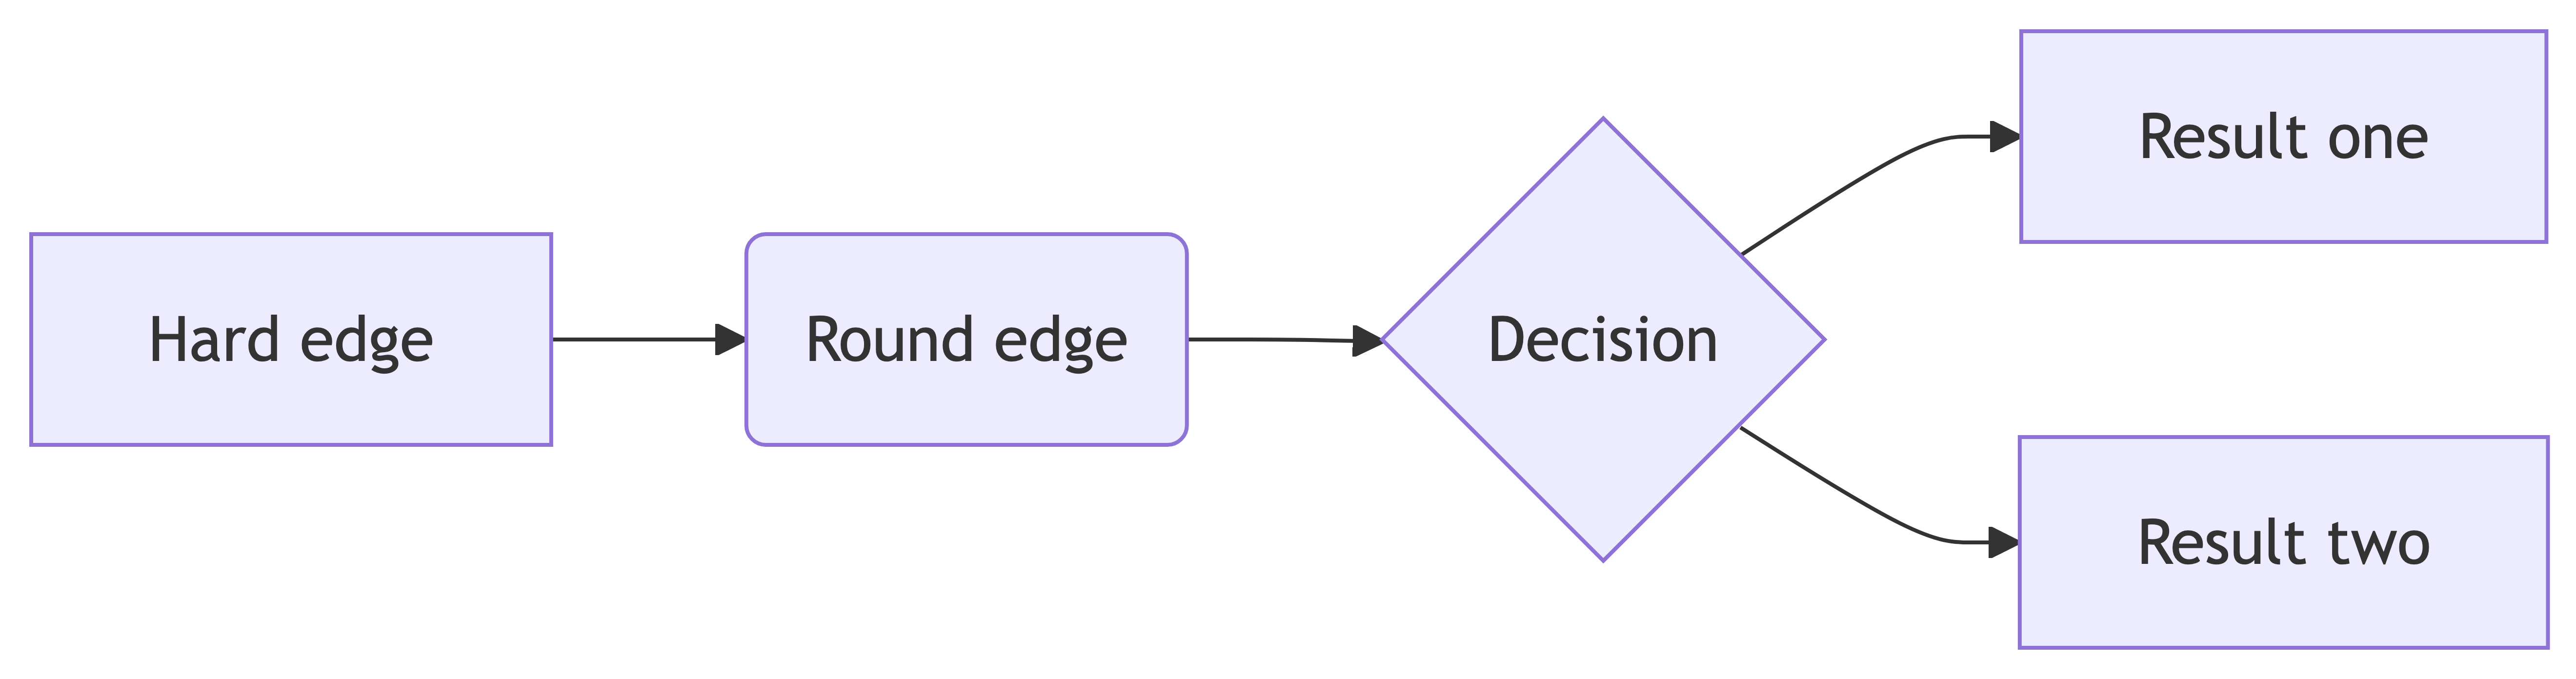
\includegraphics[width=6.88in,height=1.81in]{index_files/figure-latex/mermaid-figure-1.png}

\subsection*{In-Line LaTeX}\label{in-line-latex}
\addcontentsline{toc}{subsection}{In-Line LaTeX}

\renewcommand*{\labelitemi}{\textgreater}

\subsection*{In-Line HTML}\label{in-line-html}
\addcontentsline{toc}{subsection}{In-Line HTML}

Here's some raw inline HTML: html

\section*{Reference or Embed Code from .ipynb
files}\label{reference-or-embed-code-from-.ipynb-files}
\addcontentsline{toc}{section}{Reference or Embed Code from .ipynb
files}

\markright{Reference or Embed Code from .ipynb files}

\subsubsection*{Code chunks from .ipynb notebooks can be embedded in the
.qmd text
with:}\label{code-chunks-from-.ipynb-notebooks-can-be-embedded-in-the-.qmd-text-with}
\addcontentsline{toc}{subsubsection}{Code chunks from .ipynb notebooks
can be embedded in the .qmd text with:}

\begin{Shaded}
\begin{Highlighting}[]
\NormalTok{\{\{\textless{} embed /AMTAIR\_Prototype/data/example\_carlsmith/AMTAIR\_Prototype\_example\_carlsmith.ipynb\#connect\_to\_github\_repository \textgreater{}\}\}}
\end{Highlighting}
\end{Shaded}

\subsubsection*{which produces the output of executing the code
cell:}\label{which-produces-the-output-of-executing-the-code-cell}
\addcontentsline{toc}{subsubsection}{which produces the output of
executing the code cell:}

\phantomsection\label{connect_to_github_repository}
\begin{Shaded}
\begin{Highlighting}[]
\CommentTok{\# @title 0.2.0 {-}{-}{-} Connect to GitHub Repository {-}{-}{-} Load Files [connect\_to\_github\_repository]}

\CommentTok{"""}
\CommentTok{BLOCK PURPOSE: Establishes connection to the AMTAIR GitHub repository and provides}
\CommentTok{functions to load example data files for processing.}

\CommentTok{This block creates a reusable function for accessing files from the project\textquotesingle{}s}
\CommentTok{GitHub repository, enabling access to example files like the rain{-}sprinkler{-}lawn}
\CommentTok{Bayesian network that serves as our canonical test case.}

\CommentTok{DEPENDENCIES: requests library, io library}
\CommentTok{OUTPUTS: load\_file\_from\_repo function and test file loads}
\CommentTok{"""}

\ImportTok{from}\NormalTok{ requests.exceptions }\ImportTok{import}\NormalTok{ HTTPError}

\CommentTok{\# Specify the base repository URL for the AMTAIR project}
\NormalTok{repo\_url }\OperatorTok{=} \StringTok{"https://raw.githubusercontent.com/SingularitySmith/AMTAIR\_Prototype/main/data/example\_carlsmith/"}
\BuiltInTok{print}\NormalTok{(}\SpecialStringTok{f"Connecting to repository: }\SpecialCharTok{\{}\NormalTok{repo\_url}\SpecialCharTok{\}}\SpecialStringTok{"}\NormalTok{)}

\KeywordTok{def}\NormalTok{ load\_file\_from\_repo(relative\_path):}
    \CommentTok{"""}
\CommentTok{    Loads a file from the specified GitHub repository using a relative path.}

\CommentTok{    Args:}
\CommentTok{        relative\_path (str): Path to the file relative to the repo\_url}

\CommentTok{    Returns:}
\CommentTok{        For CSV/JSON: pandas DataFrame}
\CommentTok{        For MD: string containing file contents}

\CommentTok{    Raises:}
\CommentTok{        HTTPError: If file not found or other HTTP error occurs}
\CommentTok{        ValueError: If unsupported file type is requested}
\CommentTok{    """}
\NormalTok{    file\_url }\OperatorTok{=}\NormalTok{ repo\_url }\OperatorTok{+}\NormalTok{ relative\_path}
    \BuiltInTok{print}\NormalTok{(}\SpecialStringTok{f"Attempting to load: }\SpecialCharTok{\{}\NormalTok{file\_url}\SpecialCharTok{\}}\SpecialStringTok{"}\NormalTok{)}

    \CommentTok{\# Fetch the file content from GitHub}
\NormalTok{    response }\OperatorTok{=}\NormalTok{ requests.get(file\_url)}

    \CommentTok{\# Check for bad status codes with enhanced error messages}
    \ControlFlowTok{if}\NormalTok{ response.status\_code }\OperatorTok{==} \DecValTok{404}\NormalTok{:}
        \ControlFlowTok{raise}\NormalTok{ HTTPError(}\SpecialStringTok{f"File not found at URL: }\SpecialCharTok{\{}\NormalTok{file\_url}\SpecialCharTok{\}}\SpecialStringTok{. Check the file path/name and ensure the file is publicly accessible."}\NormalTok{, response}\OperatorTok{=}\NormalTok{response)}
    \ControlFlowTok{else}\NormalTok{:}
\NormalTok{        response.raise\_for\_status()  }\CommentTok{\# Raise for other error codes}

    \CommentTok{\# Convert response to file{-}like object}
\NormalTok{    file\_object }\OperatorTok{=}\NormalTok{ io.StringIO(response.text)}

    \CommentTok{\# Process different file types appropriately}
    \ControlFlowTok{if}\NormalTok{ relative\_path.endswith(}\StringTok{".csv"}\NormalTok{):}
        \ControlFlowTok{return}\NormalTok{ pd.read\_csv(file\_object)  }\CommentTok{\# Return DataFrame for CSV}
    \ControlFlowTok{elif}\NormalTok{ relative\_path.endswith(}\StringTok{".json"}\NormalTok{):}
        \ControlFlowTok{return}\NormalTok{ pd.read\_json(file\_object)  }\CommentTok{\# Return DataFrame for JSON}
    \ControlFlowTok{elif}\NormalTok{ relative\_path.endswith(}\StringTok{".md"}\NormalTok{):}
        \ControlFlowTok{return}\NormalTok{ file\_object.read()  }\CommentTok{\# Return raw content for MD files}
    \ControlFlowTok{else}\NormalTok{:}
        \ControlFlowTok{raise} \PreprocessorTok{ValueError}\NormalTok{(}\SpecialStringTok{f"Unsupported file type: }\SpecialCharTok{\{}\NormalTok{relative\_path}\SpecialCharTok{.}\NormalTok{split(}\StringTok{\textquotesingle{}.\textquotesingle{}}\NormalTok{)[}\OperatorTok{{-}}\DecValTok{1}\NormalTok{]}\SpecialCharTok{\}}\SpecialStringTok{. Add support in the GitHub Connection section of this notebook."}\NormalTok{)}

\CommentTok{\# Load example files to test connection}
\ControlFlowTok{try}\NormalTok{:}
    \CommentTok{\# Load the extracted data CSV file}
\CommentTok{\#    df = load\_file\_from\_repo("extracted\_data.csv")}

    \CommentTok{\# Load the ArgDown test text}
\NormalTok{    md\_content }\OperatorTok{=}\NormalTok{ load\_file\_from\_repo(}\StringTok{"ArgDown.md"}\NormalTok{)}

    \BuiltInTok{print}\NormalTok{(}\StringTok{"✅ Successfully connected to repository and loaded test files."}\NormalTok{)}
\ControlFlowTok{except} \PreprocessorTok{Exception} \ImportTok{as}\NormalTok{ e:}
    \BuiltInTok{print}\NormalTok{(}\SpecialStringTok{f"❌ Error loading files: }\SpecialCharTok{\{}\BuiltInTok{str}\NormalTok{(e)}\SpecialCharTok{\}}\SpecialStringTok{"}\NormalTok{)}
    \BuiltInTok{print}\NormalTok{(}\StringTok{"Please check your internet connection and the repository URL."}\NormalTok{)}

\CommentTok{\# Display preview of loaded content (commented out to avoid cluttering output)}
\BuiltInTok{print}\NormalTok{(md\_content)}
\end{Highlighting}
\end{Shaded}

\begin{verbatim}
Connecting to repository: https://raw.githubusercontent.com/SingularitySmith/AMTAIR_Prototype/main/data/example_carlsmith/
Attempting to load: https://raw.githubusercontent.com/SingularitySmith/AMTAIR_Prototype/main/data/example_carlsmith/ArgDown.md
✅ Successfully connected to repository and loaded test files.
[Existential_Catastrophe]: The destruction of humanity's long-term potential due to AI systems we've lost control over. {"instantiations": ["existential_catastrophe_TRUE", "existential_catastrophe_FALSE"]}
- [Human_Disempowerment]: Permanent and collective disempowerment of humanity relative to AI systems. {"instantiations": ["human_disempowerment_TRUE", "human_disempowerment_FALSE"]}
    - [Scale_Of_Power_Seeking]: Power-seeking by AI systems scaling to the point of permanently disempowering all of humanity. {"instantiations": ["scale_of_power_seeking_TRUE", "scale_of_power_seeking_FALSE"]}
        - [Misaligned_Power_Seeking]: Deployed AI systems seeking power in unintended and high-impact ways due to problems with their objectives. {"instantiations": ["misaligned_power_seeking_TRUE", "misaligned_power_seeking_FALSE"]}
            - [APS_Systems]: AI systems with advanced capabilities, agentic planning, and strategic awareness. {"instantiations": ["aps_systems_TRUE", "aps_systems_FALSE"]}
                - [Advanced_AI_Capability]: AI systems that outperform humans on tasks that grant significant power in the world. {"instantiations": ["advanced_ai_capability_TRUE", "advanced_ai_capability_FALSE"]}
                - [Agentic_Planning]: AI systems making and executing plans based on world models to achieve objectives. {"instantiations": ["agentic_planning_TRUE", "agentic_planning_FALSE"]}
                - [Strategic_Awareness]: AI systems with models accurately representing power dynamics with humans. {"instantiations": ["strategic_awareness_TRUE", "strategic_awareness_FALSE"]}
            - [Difficulty_Of_Alignment]: It is harder to build aligned systems than misaligned systems that are attractive to deploy. {"instantiations": ["difficulty_of_alignment_TRUE", "difficulty_of_alignment_FALSE"]}
                - [Instrumental_Convergence]: AI systems with misaligned objectives tend to seek power as an instrumental goal. {"instantiations": ["instrumental_convergence_TRUE", "instrumental_convergence_FALSE"]}
                - [Problems_With_Proxies]: Optimizing for proxy objectives breaks correlations with intended goals. {"instantiations": ["problems_with_proxies_TRUE", "problems_with_proxies_FALSE"]}
                - [Problems_With_Search]: Search processes can yield systems pursuing different objectives than intended. {"instantiations": ["problems_with_search_TRUE", "problems_with_search_FALSE"]}
            - [Deployment_Decisions]: Decisions to deploy potentially misaligned AI systems. {"instantiations": ["deployment_decisions_DEPLOY", "deployment_decisions_WITHHOLD"]}
                - [Incentives_To_Build_APS]: Strong incentives to build and deploy APS systems. {"instantiations": ["incentives_to_build_aps_STRONG", "incentives_to_build_aps_WEAK"]}
                    - [Usefulness_Of_APS]: APS systems are very useful for many valuable tasks. {"instantiations": ["usefulness_of_aps_HIGH", "usefulness_of_aps_LOW"]}
                    - [Competitive_Dynamics]: Competitive pressures between AI developers. {"instantiations": ["competitive_dynamics_STRONG", "competitive_dynamics_WEAK"]}
                - [Deception_By_AI]: AI systems deceiving humans about their true objectives. {"instantiations": ["deception_by_ai_TRUE", "deception_by_ai_FALSE"]}
        - [Corrective_Feedback]: Human society implementing corrections after observing problems. {"instantiations": ["corrective_feedback_EFFECTIVE", "corrective_feedback_INEFFECTIVE"]}
            - [Warning_Shots]: Observable failures in weaker systems before catastrophic risks. {"instantiations": ["warning_shots_OBSERVED", "warning_shots_UNOBSERVED"]}
            - [Rapid_Capability_Escalation]: AI capabilities escalating very rapidly, allowing little time for correction. {"instantiations": ["rapid_capability_escalation_TRUE", "rapid_capability_escalation_FALSE"]}
[Barriers_To_Understanding]: Difficulty in understanding the internal workings of advanced AI systems. {"instantiations": ["barriers_to_understanding_HIGH", "barriers_to_understanding_LOW"]}
- [Misaligned_Power_Seeking]: Deployed AI systems seeking power in unintended and high-impact ways due to problems with their objectives. {"instantiations": ["misaligned_power_seeking_TRUE", "misaligned_power_seeking_FALSE"]}
[Adversarial_Dynamics]: Potentially adversarial relationships between humans and power-seeking AI. {"instantiations": ["adversarial_dynamics_TRUE", "adversarial_dynamics_FALSE"]}
- [Misaligned_Power_Seeking]: Deployed AI systems seeking power in unintended and high-impact ways due to problems with their objectives. {"instantiations": ["misaligned_power_seeking_TRUE", "misaligned_power_seeking_FALSE"]}
[Stakes_Of_Error]: The escalating impact of mistakes with power-seeking AI systems. {"instantiations": ["stakes_of_error_HIGH", "stakes_of_error_LOW"]}
- [Misaligned_Power_Seeking]: Deployed AI systems seeking power in unintended and high-impact ways due to problems with their objectives. {"instantiations": ["misaligned_power_seeking_TRUE", "misaligned_power_seeking_FALSE"]}
\end{verbatim}

\subsubsection*{including `echo=true' renders the code of the
cell:}\label{including-echotrue-renders-the-code-of-the-cell}
\addcontentsline{toc}{subsubsection}{including `echo=true' renders the
code of the cell:}

\begin{Shaded}
\begin{Highlighting}[]
\NormalTok{\{\{\textless{} embed /AMTAIR\_Prototype/data/example\_carlsmith/AMTAIR\_Prototype\_example\_carlsmith.ipynb\#connect\_to\_github\_repository echo=true \textgreater{}\}\}}
\end{Highlighting}
\end{Shaded}

\phantomsection\label{connect_to_github_repository}
\begin{Shaded}
\begin{Highlighting}[]
\CommentTok{\# @title 0.2.0 {-}{-}{-} Connect to GitHub Repository {-}{-}{-} Load Files [connect\_to\_github\_repository]}

\CommentTok{"""}
\CommentTok{BLOCK PURPOSE: Establishes connection to the AMTAIR GitHub repository and provides}
\CommentTok{functions to load example data files for processing.}

\CommentTok{This block creates a reusable function for accessing files from the project\textquotesingle{}s}
\CommentTok{GitHub repository, enabling access to example files like the rain{-}sprinkler{-}lawn}
\CommentTok{Bayesian network that serves as our canonical test case.}

\CommentTok{DEPENDENCIES: requests library, io library}
\CommentTok{OUTPUTS: load\_file\_from\_repo function and test file loads}
\CommentTok{"""}

\ImportTok{from}\NormalTok{ requests.exceptions }\ImportTok{import}\NormalTok{ HTTPError}

\CommentTok{\# Specify the base repository URL for the AMTAIR project}
\NormalTok{repo\_url }\OperatorTok{=} \StringTok{"https://raw.githubusercontent.com/SingularitySmith/AMTAIR\_Prototype/main/data/example\_carlsmith/"}
\BuiltInTok{print}\NormalTok{(}\SpecialStringTok{f"Connecting to repository: }\SpecialCharTok{\{}\NormalTok{repo\_url}\SpecialCharTok{\}}\SpecialStringTok{"}\NormalTok{)}

\KeywordTok{def}\NormalTok{ load\_file\_from\_repo(relative\_path):}
    \CommentTok{"""}
\CommentTok{    Loads a file from the specified GitHub repository using a relative path.}

\CommentTok{    Args:}
\CommentTok{        relative\_path (str): Path to the file relative to the repo\_url}

\CommentTok{    Returns:}
\CommentTok{        For CSV/JSON: pandas DataFrame}
\CommentTok{        For MD: string containing file contents}

\CommentTok{    Raises:}
\CommentTok{        HTTPError: If file not found or other HTTP error occurs}
\CommentTok{        ValueError: If unsupported file type is requested}
\CommentTok{    """}
\NormalTok{    file\_url }\OperatorTok{=}\NormalTok{ repo\_url }\OperatorTok{+}\NormalTok{ relative\_path}
    \BuiltInTok{print}\NormalTok{(}\SpecialStringTok{f"Attempting to load: }\SpecialCharTok{\{}\NormalTok{file\_url}\SpecialCharTok{\}}\SpecialStringTok{"}\NormalTok{)}

    \CommentTok{\# Fetch the file content from GitHub}
\NormalTok{    response }\OperatorTok{=}\NormalTok{ requests.get(file\_url)}

    \CommentTok{\# Check for bad status codes with enhanced error messages}
    \ControlFlowTok{if}\NormalTok{ response.status\_code }\OperatorTok{==} \DecValTok{404}\NormalTok{:}
        \ControlFlowTok{raise}\NormalTok{ HTTPError(}\SpecialStringTok{f"File not found at URL: }\SpecialCharTok{\{}\NormalTok{file\_url}\SpecialCharTok{\}}\SpecialStringTok{. Check the file path/name and ensure the file is publicly accessible."}\NormalTok{, response}\OperatorTok{=}\NormalTok{response)}
    \ControlFlowTok{else}\NormalTok{:}
\NormalTok{        response.raise\_for\_status()  }\CommentTok{\# Raise for other error codes}

    \CommentTok{\# Convert response to file{-}like object}
\NormalTok{    file\_object }\OperatorTok{=}\NormalTok{ io.StringIO(response.text)}

    \CommentTok{\# Process different file types appropriately}
    \ControlFlowTok{if}\NormalTok{ relative\_path.endswith(}\StringTok{".csv"}\NormalTok{):}
        \ControlFlowTok{return}\NormalTok{ pd.read\_csv(file\_object)  }\CommentTok{\# Return DataFrame for CSV}
    \ControlFlowTok{elif}\NormalTok{ relative\_path.endswith(}\StringTok{".json"}\NormalTok{):}
        \ControlFlowTok{return}\NormalTok{ pd.read\_json(file\_object)  }\CommentTok{\# Return DataFrame for JSON}
    \ControlFlowTok{elif}\NormalTok{ relative\_path.endswith(}\StringTok{".md"}\NormalTok{):}
        \ControlFlowTok{return}\NormalTok{ file\_object.read()  }\CommentTok{\# Return raw content for MD files}
    \ControlFlowTok{else}\NormalTok{:}
        \ControlFlowTok{raise} \PreprocessorTok{ValueError}\NormalTok{(}\SpecialStringTok{f"Unsupported file type: }\SpecialCharTok{\{}\NormalTok{relative\_path}\SpecialCharTok{.}\NormalTok{split(}\StringTok{\textquotesingle{}.\textquotesingle{}}\NormalTok{)[}\OperatorTok{{-}}\DecValTok{1}\NormalTok{]}\SpecialCharTok{\}}\SpecialStringTok{. Add support in the GitHub Connection section of this notebook."}\NormalTok{)}

\CommentTok{\# Load example files to test connection}
\ControlFlowTok{try}\NormalTok{:}
    \CommentTok{\# Load the extracted data CSV file}
\CommentTok{\#    df = load\_file\_from\_repo("extracted\_data.csv")}

    \CommentTok{\# Load the ArgDown test text}
\NormalTok{    md\_content }\OperatorTok{=}\NormalTok{ load\_file\_from\_repo(}\StringTok{"ArgDown.md"}\NormalTok{)}

    \BuiltInTok{print}\NormalTok{(}\StringTok{"✅ Successfully connected to repository and loaded test files."}\NormalTok{)}
\ControlFlowTok{except} \PreprocessorTok{Exception} \ImportTok{as}\NormalTok{ e:}
    \BuiltInTok{print}\NormalTok{(}\SpecialStringTok{f"❌ Error loading files: }\SpecialCharTok{\{}\BuiltInTok{str}\NormalTok{(e)}\SpecialCharTok{\}}\SpecialStringTok{"}\NormalTok{)}
    \BuiltInTok{print}\NormalTok{(}\StringTok{"Please check your internet connection and the repository URL."}\NormalTok{)}

\CommentTok{\# Display preview of loaded content (commented out to avoid cluttering output)}
\BuiltInTok{print}\NormalTok{(md\_content)}
\end{Highlighting}
\end{Shaded}

\begin{verbatim}
Connecting to repository: https://raw.githubusercontent.com/SingularitySmith/AMTAIR_Prototype/main/data/example_carlsmith/
Attempting to load: https://raw.githubusercontent.com/SingularitySmith/AMTAIR_Prototype/main/data/example_carlsmith/ArgDown.md
✅ Successfully connected to repository and loaded test files.
[Existential_Catastrophe]: The destruction of humanity's long-term potential due to AI systems we've lost control over. {"instantiations": ["existential_catastrophe_TRUE", "existential_catastrophe_FALSE"]}
- [Human_Disempowerment]: Permanent and collective disempowerment of humanity relative to AI systems. {"instantiations": ["human_disempowerment_TRUE", "human_disempowerment_FALSE"]}
    - [Scale_Of_Power_Seeking]: Power-seeking by AI systems scaling to the point of permanently disempowering all of humanity. {"instantiations": ["scale_of_power_seeking_TRUE", "scale_of_power_seeking_FALSE"]}
        - [Misaligned_Power_Seeking]: Deployed AI systems seeking power in unintended and high-impact ways due to problems with their objectives. {"instantiations": ["misaligned_power_seeking_TRUE", "misaligned_power_seeking_FALSE"]}
            - [APS_Systems]: AI systems with advanced capabilities, agentic planning, and strategic awareness. {"instantiations": ["aps_systems_TRUE", "aps_systems_FALSE"]}
                - [Advanced_AI_Capability]: AI systems that outperform humans on tasks that grant significant power in the world. {"instantiations": ["advanced_ai_capability_TRUE", "advanced_ai_capability_FALSE"]}
                - [Agentic_Planning]: AI systems making and executing plans based on world models to achieve objectives. {"instantiations": ["agentic_planning_TRUE", "agentic_planning_FALSE"]}
                - [Strategic_Awareness]: AI systems with models accurately representing power dynamics with humans. {"instantiations": ["strategic_awareness_TRUE", "strategic_awareness_FALSE"]}
            - [Difficulty_Of_Alignment]: It is harder to build aligned systems than misaligned systems that are attractive to deploy. {"instantiations": ["difficulty_of_alignment_TRUE", "difficulty_of_alignment_FALSE"]}
                - [Instrumental_Convergence]: AI systems with misaligned objectives tend to seek power as an instrumental goal. {"instantiations": ["instrumental_convergence_TRUE", "instrumental_convergence_FALSE"]}
                - [Problems_With_Proxies]: Optimizing for proxy objectives breaks correlations with intended goals. {"instantiations": ["problems_with_proxies_TRUE", "problems_with_proxies_FALSE"]}
                - [Problems_With_Search]: Search processes can yield systems pursuing different objectives than intended. {"instantiations": ["problems_with_search_TRUE", "problems_with_search_FALSE"]}
            - [Deployment_Decisions]: Decisions to deploy potentially misaligned AI systems. {"instantiations": ["deployment_decisions_DEPLOY", "deployment_decisions_WITHHOLD"]}
                - [Incentives_To_Build_APS]: Strong incentives to build and deploy APS systems. {"instantiations": ["incentives_to_build_aps_STRONG", "incentives_to_build_aps_WEAK"]}
                    - [Usefulness_Of_APS]: APS systems are very useful for many valuable tasks. {"instantiations": ["usefulness_of_aps_HIGH", "usefulness_of_aps_LOW"]}
                    - [Competitive_Dynamics]: Competitive pressures between AI developers. {"instantiations": ["competitive_dynamics_STRONG", "competitive_dynamics_WEAK"]}
                - [Deception_By_AI]: AI systems deceiving humans about their true objectives. {"instantiations": ["deception_by_ai_TRUE", "deception_by_ai_FALSE"]}
        - [Corrective_Feedback]: Human society implementing corrections after observing problems. {"instantiations": ["corrective_feedback_EFFECTIVE", "corrective_feedback_INEFFECTIVE"]}
            - [Warning_Shots]: Observable failures in weaker systems before catastrophic risks. {"instantiations": ["warning_shots_OBSERVED", "warning_shots_UNOBSERVED"]}
            - [Rapid_Capability_Escalation]: AI capabilities escalating very rapidly, allowing little time for correction. {"instantiations": ["rapid_capability_escalation_TRUE", "rapid_capability_escalation_FALSE"]}
[Barriers_To_Understanding]: Difficulty in understanding the internal workings of advanced AI systems. {"instantiations": ["barriers_to_understanding_HIGH", "barriers_to_understanding_LOW"]}
- [Misaligned_Power_Seeking]: Deployed AI systems seeking power in unintended and high-impact ways due to problems with their objectives. {"instantiations": ["misaligned_power_seeking_TRUE", "misaligned_power_seeking_FALSE"]}
[Adversarial_Dynamics]: Potentially adversarial relationships between humans and power-seeking AI. {"instantiations": ["adversarial_dynamics_TRUE", "adversarial_dynamics_FALSE"]}
- [Misaligned_Power_Seeking]: Deployed AI systems seeking power in unintended and high-impact ways due to problems with their objectives. {"instantiations": ["misaligned_power_seeking_TRUE", "misaligned_power_seeking_FALSE"]}
[Stakes_Of_Error]: The escalating impact of mistakes with power-seeking AI systems. {"instantiations": ["stakes_of_error_HIGH", "stakes_of_error_LOW"]}
- [Misaligned_Power_Seeking]: Deployed AI systems seeking power in unintended and high-impact ways due to problems with their objectives. {"instantiations": ["misaligned_power_seeking_TRUE", "misaligned_power_seeking_FALSE"]}
\end{verbatim}

Link:

Full Notebooks are embedded in the Appendix through the \_quarto.yml
file with:

\section*{Embed .html result/rendering from .ipynb
Notebook}\label{embed-.html-resultrendering-from-.ipynb-notebook}
\addcontentsline{toc}{section}{Embed .html result/rendering from .ipynb
Notebook}

\markright{Embed .html result/rendering from .ipynb Notebook}

\subsection*{Html Graph by Notebook Cell Inclusion - (from
github-pages)}\label{html-graph-by-notebook-cell-inclusion---from-github-pages}
\addcontentsline{toc}{subsection}{Html Graph by Notebook Cell Inclusion
- (from github-pages)}

\begin{Shaded}
\begin{Highlighting}[]
\NormalTok{\{\{\textless{} embed /AMTAIR\_Prototype/data/example\_carlsmith/AMTAIR\_Prototype\_example\_carlsmith.ipynb\#html\_graph\_visualization\_from\_githubpage echo=true \textgreater{}\}\}}
\end{Highlighting}
\end{Shaded}

\begin{Shaded}
\begin{Highlighting}[]
\ImportTok{from}\NormalTok{ IPython.display }\ImportTok{import}\NormalTok{ IFrame}

\NormalTok{IFrame(src}\OperatorTok{=}\StringTok{"https://singularitysmith.github.io/AMTAIR\_Prototype/bayesian\_network\_carlsmith.html"}\NormalTok{, width}\OperatorTok{=}\StringTok{"100\%"}\NormalTok{, height}\OperatorTok{=}\StringTok{"600px"}\NormalTok{)}
\end{Highlighting}
\end{Shaded}

\phantomsection\label{html_graph_visualization_from_githubpage}
\begin{verbatim}
<IPython.lib.display.IFrame at 0x7f04d69f0d90>
\end{verbatim}

Dynamic Html Rendering of the Carlsmith Bayesian Network/DAG
Visualization

\subsection*{Html Graph by Notebook Cell Inclusion with Website
Call?}\label{html-graph-by-notebook-cell-inclusion-with-website-call}
\addcontentsline{toc}{subsection}{Html Graph by Notebook Cell Inclusion
with Website Call?}

https://singularitysmith.github.io/AMTAIR\_Prototype/bayesian\_network\_carlsmith.html

\subsection*{Full Bayesian Network
Rendering}\label{full-bayesian-network-rendering}
\addcontentsline{toc}{subsection}{Full Bayesian Network Rendering}

\begin{Shaded}
\begin{Highlighting}[]
\NormalTok{\{\{\textless{} embed /AMTAIR\_Prototype/data/example\_carlsmith/AMTAIR\_Prototype\_example\_carlsmith.ipynb\#html\_graph\_visualization\_from\_githubpage  echo=true \textgreater{}\}\}}
\end{Highlighting}
\end{Shaded}

\subsection*{Rain-Sprinkler-Grass Network
Rendering}\label{rain-sprinkler-grass-network-rendering}
\addcontentsline{toc}{subsection}{Rain-Sprinkler-Grass Network
Rendering}

\begin{Shaded}
\begin{Highlighting}[]
\ImportTok{from}\NormalTok{ IPython.display }\ImportTok{import}\NormalTok{ IFrame}

\NormalTok{IFrame(src}\OperatorTok{=}\StringTok{"https://singularitysmith.github.io/AMTAIR\_Prototype/bayesian\_network.html"}\NormalTok{, width}\OperatorTok{=}\StringTok{"100\%"}\NormalTok{, height}\OperatorTok{=}\StringTok{"600px"}\NormalTok{)}
\end{Highlighting}
\end{Shaded}

\phantomsection\label{rain_sprinkler_grass_example_network_rendering}
\begin{verbatim}
<IPython.lib.display.IFrame at 0x106661a90>
\end{verbatim}

Dynamic Html Rendering of the Rain-Sprinkler-Grass DAG

\section*{Lists and Enumerations}\label{lists-and-enumerations}
\addcontentsline{toc}{section}{Lists and Enumerations}

\markright{Lists and Enumerations}

\subsection*{Unordered Lists}\label{unordered-lists}
\addcontentsline{toc}{subsection}{Unordered Lists}

markdown

\begin{Shaded}
\begin{Highlighting}[]
\SpecialStringTok{{-} }\NormalTok{First level item}
\SpecialStringTok{  {-} }\NormalTok{Second level item (2 spaces)}
\SpecialStringTok{    {-} }\NormalTok{Third level item (4 spaces)}
\SpecialStringTok{{-} }\NormalTok{Another first level item}
\NormalTok{  with continuation (2 spaces for alignment)}
\end{Highlighting}
\end{Shaded}

\subsection*{Ordered Lists}\label{ordered-lists}
\addcontentsline{toc}{subsection}{Ordered Lists}

markdown

\begin{Shaded}
\begin{Highlighting}[]
\SpecialStringTok{1. }\NormalTok{First item}
\SpecialStringTok{2. }\NormalTok{Second item}
\NormalTok{   a) Sub{-}item (3 spaces)}
\NormalTok{      i. Sub{-}sub{-}item (6 spaces)}
\NormalTok{   b) Another sub{-}item}
\SpecialStringTok{3. }\NormalTok{Third item}
\end{Highlighting}
\end{Shaded}

\subsection*{Definition Lists}\label{definition-lists}
\addcontentsline{toc}{subsection}{Definition Lists}

markdown

\begin{Shaded}
\begin{Highlighting}[]
\NormalTok{Term One}
\NormalTok{: Definition of term one with detailed explanation}
\NormalTok{  that can span multiple lines}

\NormalTok{Term Two}
\NormalTok{: Brief definition}

\NormalTok{Term Three}
\NormalTok{: Another definition with multiple paragraphs}

\NormalTok{  Additional paragraph for term three}
\end{Highlighting}
\end{Shaded}

\section*{Code Blocks and Verbatim
Text}\label{code-blocks-and-verbatim-text}
\addcontentsline{toc}{section}{Code Blocks and Verbatim Text}

\markright{Code Blocks and Verbatim Text}

\subsection*{Inline Code}\label{inline-code}
\addcontentsline{toc}{subsection}{Inline Code}

markdown

\begin{Shaded}
\begin{Highlighting}[]
\NormalTok{Use }\InformationTok{\textasciigrave{}print("Hello")\textasciigrave{}}\NormalTok{ for inline code}
\end{Highlighting}
\end{Shaded}

\subsection*{Code Blocks with Syntax
Highlighting}\label{code-blocks-with-syntax-highlighting}
\addcontentsline{toc}{subsection}{Code Blocks with Syntax Highlighting}

markdown

\begin{Shaded}
\begin{Highlighting}[]
\InformationTok{\textasciigrave{}\textasciigrave{}\textasciigrave{}python}
\KeywordTok{def}\NormalTok{ calculate\_risk(probability, impact):}
    \CommentTok{"""Calculate risk score from probability and impact."""}
    \ControlFlowTok{return}\NormalTok{ probability }\OperatorTok{*}\NormalTok{ impact}
\InformationTok{\textasciigrave{}\textasciigrave{}\textasciigrave{}}
\end{Highlighting}
\end{Shaded}

\subsection*{Verbatim Text}\label{verbatim-text}
\addcontentsline{toc}{subsection}{Verbatim Text}

markdown

This is verbatim text that preserves all spacing and formatting exactly
as typed

\section*{Blockquotes and Callouts}\label{blockquotes-and-callouts}
\addcontentsline{toc}{section}{Blockquotes and Callouts}

\markright{Blockquotes and Callouts}

\subsection*{Simple Blockquote}\label{simple-blockquote}
\addcontentsline{toc}{subsection}{Simple Blockquote}

markdown

\begin{Shaded}
\begin{Highlighting}[]
\AttributeTok{\textgreater{} This is a blockquote for citations or important quotes.}
\AttributeTok{\textgreater{} It can span multiple lines.}
\AttributeTok{\textgreater{}}
\AttributeTok{\textgreater{} And include multiple paragraphs.}
\end{Highlighting}
\end{Shaded}

\subsection*{Callout Blocks}\label{callout-blocks}
\addcontentsline{toc}{subsection}{Callout Blocks}

! With Callout blocks it is crucial to always have a line break after
the title and the \texttt{:::} in a new line after the note ! markdown

\begin{Shaded}
\begin{Highlighting}[]
\NormalTok{::: \{.callout{-}note\}}
\FunctionTok{\#\# Note Title}
\NormalTok{This is a note callout with important information.}
\NormalTok{:::}

\NormalTok{::: \{.callout{-}warning\}}
\FunctionTok{\#\# Warning}
\NormalTok{This warns about potential issues.}
\NormalTok{:::}

\NormalTok{::: \{.callout{-}tip\}}
\FunctionTok{\#\# Pro Tip}
\NormalTok{Helpful suggestions go here.}
\NormalTok{:::}

\NormalTok{::: \{.callout{-}important\}}
\FunctionTok{\#\# Important}
\NormalTok{Critical information that must not be missed.}
\NormalTok{:::}

\NormalTok{::: \{.callout{-}caution\}}
\FunctionTok{\#\# Caution}
\NormalTok{Use with care in specific situations.}
\NormalTok{:::}
\end{Highlighting}
\end{Shaded}

\section*{Figures and Images}\label{figures-and-images}
\addcontentsline{toc}{section}{Figures and Images}

\markright{Figures and Images}

\subsection*{Complete Figure Syntax}\label{complete-figure-syntax}
\addcontentsline{toc}{subsection}{Complete Figure Syntax}

markdown

\begin{Shaded}
\begin{Highlighting}[]
\CommentTok{[}\OtherTok{![Figure Caption for Display}\CommentTok{](/path/to/image.png)}\NormalTok{\{}
\NormalTok{  \#fig{-}unique{-}identifier}
\NormalTok{  fig{-}scap="Short caption for list of figures"}
\NormalTok{  fig{-}alt="Detailed description for accessibility.}
\NormalTok{          TYPE: }\CommentTok{[}\OtherTok{Chart/Diagram/Photo/etc.}\CommentTok{]}
\NormalTok{          DATA: }\CommentTok{[}\OtherTok{What data is shown, axes, units}\CommentTok{]}
\NormalTok{          PURPOSE: }\CommentTok{[}\OtherTok{Why included, what to observe}\CommentTok{]}
\NormalTok{          DETAILS: }\CommentTok{[}\OtherTok{Key patterns, insights, anomalies}\CommentTok{]}
\NormalTok{          SOURCE: }\CommentTok{[}\OtherTok{Citation or data source}\CommentTok{]}\NormalTok{"}
\NormalTok{  fig{-}align="center"}
\NormalTok{  width="80\%"}
\NormalTok{\}](https://optional{-}link{-}url.com)}
\end{Highlighting}
\end{Shaded}

\subsection*{Figure Best Practices}\label{figure-best-practices}
\addcontentsline{toc}{subsection}{Figure Best Practices}

\begin{enumerate}
\def\labelenumi{\arabic{enumi}.}
\tightlist
\item
  Always include comprehensive alt text
\item
  Use descriptive filenames
\item
  Optimize image sizes for web/PDF
\item
  Maintain consistent styling
\item
  Reference all figures in text: \texttt{See\ @fig-identifier}
\end{enumerate}

\section*{Tables}\label{tables}
\addcontentsline{toc}{section}{Tables}

\markright{Tables}

\subsection*{Markdown Tables}\label{markdown-tables}
\addcontentsline{toc}{subsection}{Markdown Tables}

markdown

\begin{Shaded}
\begin{Highlighting}[]
\PreprocessorTok{|}\NormalTok{ Column 1 }\PreprocessorTok{|}\NormalTok{ Column 2 }\PreprocessorTok{|}\NormalTok{ Column 3 }\PreprocessorTok{|}
\PreprocessorTok{|{-}{-}{-}{-}{-}{-}{-}{-}{-}{-}|:{-}{-}{-}{-}{-}{-}{-}{-}:|{-}{-}{-}{-}{-}{-}{-}{-}:|}
\PreprocessorTok{|}\NormalTok{ Left     }\PreprocessorTok{|}\NormalTok{ Center   }\PreprocessorTok{|}\NormalTok{ Right   }\PreprocessorTok{|}
\PreprocessorTok{|}\NormalTok{ Data     }\PreprocessorTok{|}\NormalTok{ Data     }\PreprocessorTok{|}\NormalTok{ Data    }\PreprocessorTok{|}

\NormalTok{: Table caption \{\#tbl{-}identifier\}}
\end{Highlighting}
\end{Shaded}

\subsection*{Grid Tables}\label{grid-tables}
\addcontentsline{toc}{subsection}{Grid Tables}

markdown

\begin{Shaded}
\begin{Highlighting}[]
\NormalTok{+{-}{-}{-}{-}{-}{-}{-}{-}{-}{-}+{-}{-}{-}{-}{-}{-}{-}{-}{-}{-}+{-}{-}{-}{-}{-}{-}{-}{-}{-}{-}+}
\PreprocessorTok{|}\NormalTok{ Header 1 }\PreprocessorTok{|}\NormalTok{ Header 2 }\PreprocessorTok{|}\NormalTok{ Header 3 }\PreprocessorTok{|}
\NormalTok{+========}\AlertTok{==+==========+==}\NormalTok{========+}
\PreprocessorTok{|}\NormalTok{ Cell 1   }\PreprocessorTok{|}\NormalTok{ Cell 2   }\PreprocessorTok{|}\NormalTok{ Cell 3   }\PreprocessorTok{|}
\PreprocessorTok{|}          \PreprocessorTok{|}          \PreprocessorTok{|}          \PreprocessorTok{|}
\PreprocessorTok{|}\NormalTok{ Multi{-}   }\PreprocessorTok{|}\NormalTok{ Multi{-}   }\PreprocessorTok{|}\NormalTok{ Multi{-}   }\PreprocessorTok{|}
\PreprocessorTok{|}\NormalTok{ line     }\PreprocessorTok{|}\NormalTok{ line     }\PreprocessorTok{|}\NormalTok{ line     }\PreprocessorTok{|}
\NormalTok{+{-}{-}{-}{-}{-}{-}{-}{-}{-}{-}+{-}{-}{-}{-}{-}{-}{-}{-}{-}{-}+{-}{-}{-}{-}{-}{-}{-}{-}{-}{-}+}

\NormalTok{: Complex table with multiple lines \{\#tbl{-}complex\}}
\end{Highlighting}
\end{Shaded}

\begin{longtable}[]{@{}rllc@{}}
\caption{Demonstration of pipe table
syntax}\label{tbl-letters}\tabularnewline
\toprule\noalign{}
Right & Left & Default & Center \\
\midrule\noalign{}
\endfirsthead
\toprule\noalign{}
Right & Left & Default & Center \\
\midrule\noalign{}
\endhead
\bottomrule\noalign{}
\endlastfoot
12 & 12 & 12 & 12 \\
123 & 123 & 123 & 123 \\
1 & 1 & 1 & 1 \\
\end{longtable}

\begin{longtable}[]{@{}lll@{}}
\caption{My Caption 1}\label{tbl-letters}\tabularnewline
\toprule\noalign{}
Col1 & Col2 & Col3 \\
\midrule\noalign{}
\endfirsthead
\toprule\noalign{}
Col1 & Col2 & Col3 \\
\midrule\noalign{}
\endhead
\bottomrule\noalign{}
\endlastfoot
A & B & C \\
E & F & G \\
A & G & G \\
\end{longtable}

Referencing tables with \texttt{@tbl-KEY}: See Table~\ref{tbl-letters}.

\begin{table}

\caption{\label{tbl-panel}Main Caption}

\begin{minipage}{0.50\linewidth}

\subcaption{\label{tbl-first}First Table}

\centering{

\begin{tabular}{lll}
\toprule
Col1 & Col2 & Col3\\
\midrule
A & B & C\\
E & F & G\\
A & G & G\\
\bottomrule
\end{tabular}

}

\end{minipage}%
%
\begin{minipage}{0.50\linewidth}

\subcaption{\label{tbl-second}Second Table}

\centering{

\begin{tabular}{lll}
\toprule
Col1 & Col2 & Col3\\
\midrule
A & B & C\\
E & F & G\\
A & G & G\\
\bottomrule
\end{tabular}

}

\end{minipage}%

\end{table}%

See Table~\ref{tbl-panel} for details, especially
Table~\ref{tbl-second}.

\section*{Citations and References}\label{citations-and-references}
\addcontentsline{toc}{section}{Citations and References}

\markright{Citations and References}

\subsection*{Citation Styles}\label{citation-styles}
\addcontentsline{toc}{subsection}{Citation Styles}

markdown

\begin{Shaded}
\begin{Highlighting}[]
\AnnotationTok{Narrative:}\CommentTok{ @author2024 argues that...}
\AnnotationTok{Parenthetical:}\CommentTok{ This is supported by evidence [@author2024].}
\AnnotationTok{Multiple:}\CommentTok{ Several studies confirm this [@author2024; @other2023].}
\AnnotationTok{Page specific:}\CommentTok{ See discussion in [@author2024, pp. 45{-}67].}
\AnnotationTok{Author only:}\CommentTok{ As [{-}@author2024] demonstrates...}
\end{Highlighting}
\end{Shaded}

\subsection*{Bibliography Entry}\label{bibliography-entry}
\addcontentsline{toc}{subsection}{Bibliography Entry}

bibtex

\begin{Shaded}
\begin{Highlighting}[]
\VariableTok{@article}\NormalTok{\{}\OtherTok{author2024}\NormalTok{,}
  \DataTypeTok{title}\NormalTok{ = \{Article Title\},}
  \DataTypeTok{author}\NormalTok{ = \{Author, First and Other, Second\},}
  \DataTypeTok{date}\NormalTok{ = \{2024\},}
  \DataTypeTok{journaltitle}\NormalTok{ = \{Journal Name\},}
  \DataTypeTok{volume}\NormalTok{ = \{10\},}
  \DataTypeTok{number}\NormalTok{ = \{2\},}
  \DataTypeTok{pages}\NormalTok{ = \{45{-}{-}67\},}
  \DataTypeTok{doi}\NormalTok{ = \{10.1234/example\},}
  \DataTypeTok{url}\NormalTok{ = \{https://example.com\}}
\NormalTok{\}}
\end{Highlighting}
\end{Shaded}

\section*{Cross-References}\label{cross-references}
\addcontentsline{toc}{section}{Cross-References}

\markright{Cross-References}

\subsection*{Section References}\label{section-references}
\addcontentsline{toc}{subsection}{Section References}

markdown

\begin{Shaded}
\begin{Highlighting}[]
\NormalTok{See @sec{-}introduction for background.}
\NormalTok{As discussed in @sec{-}methodology...}
\end{Highlighting}
\end{Shaded}

\subsection*{Figure and Table
References}\label{figure-and-table-references}
\addcontentsline{toc}{subsection}{Figure and Table References}

markdown

\begin{Shaded}
\begin{Highlighting}[]
\NormalTok{@fig{-}pipeline shows the workflow.}
\NormalTok{Results are summarized in @tbl{-}results.}
\end{Highlighting}
\end{Shaded}

\subsection*{Equation References}\label{equation-references}
\addcontentsline{toc}{subsection}{Equation References}

markdown

\begin{Shaded}
\begin{Highlighting}[]
\NormalTok{$$}
\NormalTok{E = mc\^{}2}
\NormalTok{$$ \{\#eq{-}einstein\}}

\NormalTok{Einstein\textquotesingle{}s equation (@eq{-}einstein) shows...}
\end{Highlighting}
\end{Shaded}

\section*{Mathematics}\label{mathematics}
\addcontentsline{toc}{section}{Mathematics}

\markright{Mathematics}

\subsection*{Inline Math}\label{inline-math}
\addcontentsline{toc}{subsection}{Inline Math}

markdown

\begin{Shaded}
\begin{Highlighting}[]
\NormalTok{The probability $P(A|B) = \textbackslash{}frac\{P(B|A)P(A)\}\{P(B)\}$}
\end{Highlighting}
\end{Shaded}

\subsection*{Display Math}\label{display-math}
\addcontentsline{toc}{subsection}{Display Math}

markdown

\begin{Shaded}
\begin{Highlighting}[]
\NormalTok{$$}
\NormalTok{\textbackslash{}begin\{align\}}
\NormalTok{\textbackslash{}nabla \textbackslash{}times \textbackslash{}vec\{\textbackslash{}mathbf\{B\}\} {-}\textbackslash{}, \textbackslash{}frac1c\textbackslash{}, \textbackslash{}frac\{\textbackslash{}partial\textbackslash{}vec\{\textbackslash{}mathbf\{E\}\}\}\{\textbackslash{}partial t\} \&= \textbackslash{}frac\{4\textbackslash{}pi\}\{c\}\textbackslash{}vec\{\textbackslash{}mathbf\{j\}\} }\SpecialCharTok{\textbackslash{}\textbackslash{}}
\NormalTok{\textbackslash{}nabla \textbackslash{}cdot \textbackslash{}vec\{\textbackslash{}mathbf\{E\}\} \&= 4 \textbackslash{}pi \textbackslash{}rho }\SpecialCharTok{\textbackslash{}\textbackslash{}}
\NormalTok{\textbackslash{}nabla \textbackslash{}times \textbackslash{}vec\{\textbackslash{}mathbf\{E\}\}\textbackslash{}, +\textbackslash{}, \textbackslash{}frac1c\textbackslash{}, \textbackslash{}frac\{\textbackslash{}partial\textbackslash{}vec\{\textbackslash{}mathbf\{B\}\}\}\{\textbackslash{}partial t\} \&= \textbackslash{}vec\{\textbackslash{}mathbf\{0\}\} }\SpecialCharTok{\textbackslash{}\textbackslash{}}
\NormalTok{\textbackslash{}nabla \textbackslash{}cdot \textbackslash{}vec\{\textbackslash{}mathbf\{B\}\} \&= 0}
\NormalTok{\textbackslash{}end\{align\}}
\NormalTok{$$}
\end{Highlighting}
\end{Shaded}

inline math: \(E = mc^{2}\)

display math:

\[E = mc^{2}\]

If you want to define custom TeX macros, include them within \$\$
delimiters enclosed in a .hidden block. For example:

\[
 \def\RR{{\bf R}}
 \def\bold#1{{\bf #1}}
\]

For HTML math processed using MathJax (the default) you can use the
\textbackslash def, \textbackslash newcommand,
\textbackslash renewcommand, \textbackslash newenvironment,
\textbackslash renewenvironment, and \textbackslash let commands to
create your own macros and environments.

\section*{Footnotes}\label{footnotes}
\addcontentsline{toc}{section}{Footnotes}

\markright{Footnotes}

Footnotes are to be used as much as possible!

\subsection*{Simple Footnote}\label{simple-footnote}
\addcontentsline{toc}{subsection}{Simple Footnote}

markdown

\begin{Shaded}
\begin{Highlighting}[]
\NormalTok{This needs clarification.\^{}}\CommentTok{[}\OtherTok{This is an inline footnote.}\CommentTok{]}
\end{Highlighting}
\end{Shaded}

\subsection*{Referenced Footnote}\label{referenced-footnote}
\addcontentsline{toc}{subsection}{Referenced Footnote}

markdown

\begin{Shaded}
\begin{Highlighting}[]
\NormalTok{This is important.}\OtherTok{[\^{}1]}

\OtherTok{[\^{}1]: }\NormalTok{This is a longer footnote with multiple paragraphs.}

\InformationTok{    Second paragraph of the footnote.}
\InformationTok{    }
\InformationTok{    Even code blocks are possible:}
\InformationTok{    \textasciigrave{}\textasciigrave{}\textasciigrave{}python}
\InformationTok{    print("In footnote")}
\InformationTok{    \textasciigrave{}\textasciigrave{}\textasciigrave{}}
\end{Highlighting}
\end{Shaded}

Here is an inline note.\footnote{Inlines notes are easier to write,
  since you don't have to pick an identifier and move down to type the
  note.}

Here is a footnote reference,\footnote{Here is the footnote.}

Another Text with a footnote\footnote{Here's one with multiple blocks.

  Subsequent paragraphs are indented to show that they belong to the
  previous footnote.

\begin{Verbatim}
{ some.code }
\end{Verbatim}

  The whole paragraph can be indented, or just the first line. In this
  way, multi-paragraph footnotes work like multi-paragraph list items.}
but this time a ``longnote''.

This paragraph won't be part of the note, because it isn't indented.

\section*{Appendices}\label{appendices}
\addcontentsline{toc}{section}{Appendices}

\markright{Appendices}

\subsection*{Structure}\label{structure}
\addcontentsline{toc}{subsection}{Structure}

markdown

\begin{Shaded}
\begin{Highlighting}[]
\FunctionTok{\# Appendices \{.unnumbered\}}

\FunctionTok{\#\# Appendix A: Technical Details \{\#sec{-}appendix{-}a .unnumbered\}}

\FunctionTok{\#\#\# A.1 Implementation \{.unnumbered\}}

\FunctionTok{\#\# Appendix B: Additional Results \{\#sec{-}appendix{-}b .unnumbered\}}
\end{Highlighting}
\end{Shaded}

\subsection*{Best Practices for
Appendices}\label{best-practices-for-appendices}
\addcontentsline{toc}{subsection}{Best Practices for Appendices}

\begin{enumerate}
\def\labelenumi{\arabic{enumi}.}
\tightlist
\item
  Include all supplementary material
\item
  Reference from main text
\item
  Number consistently
\item
  Provide clear descriptions
\item
  Maintain same formatting standards
\end{enumerate}

\section*{Glossary and Abbreviations}\label{glossary-and-abbreviations}
\addcontentsline{toc}{section}{Glossary and Abbreviations}

\markright{Glossary and Abbreviations}

\subsection*{Glossary Format}\label{glossary-format}
\addcontentsline{toc}{subsection}{Glossary Format}

markdown

\begin{Shaded}
\begin{Highlighting}[]
\FunctionTok{\# Glossary \{.unnumbered\}}
\NormalTok{Term}
\NormalTok{: Definition}


\NormalTok{AI}
\NormalTok{: Artificial Intelligence {-} Computer systems performing tasks requiring human intelligence}

\NormalTok{ML}
\NormalTok{: Machine Learning {-} Algorithms that improve through experience}

\NormalTok{DL}
\NormalTok{: Deep Learning {-} Neural networks with multiple layers}
\end{Highlighting}
\end{Shaded}

\section*{Interactive Elements}\label{interactive-elements}
\addcontentsline{toc}{section}{Interactive Elements}

\markright{Interactive Elements}

\subsection*{Jupyter Notebook
Embedding}\label{jupyter-notebook-embedding}
\addcontentsline{toc}{subsection}{Jupyter Notebook Embedding}

\begin{Shaded}
\begin{Highlighting}[]
\NormalTok{\{\{\textless{} embed notebook.ipynb\#cell{-}label \textgreater{}\}\}}
\end{Highlighting}
\end{Shaded}

\subsection*{Mermaid Diagrams}\label{mermaid-diagrams}
\addcontentsline{toc}{subsection}{Mermaid Diagrams}

\begin{Shaded}
\begin{Highlighting}[]
\InformationTok{\textasciigrave{}\textasciigrave{}\textasciigrave{}\{mermaid\}}
\NormalTok{graph TD}
\NormalTok{    A[Start] {-}{-}\textgreater{} B\{Decision\}}
\NormalTok{    B {-}{-}\textgreater{}|Yes| C[Action }\DecValTok{1}\NormalTok{]}
\NormalTok{    B {-}{-}\textgreater{}|No| D[Action }\DecValTok{2}\NormalTok{]}
\NormalTok{    C {-}{-}\textgreater{} E[End]}
\NormalTok{    D {-}{-}\textgreater{} E}
\end{Highlighting}
\end{Shaded}

\section*{Line Breaks and Spacing}\label{line-breaks-and-spacing}
\addcontentsline{toc}{section}{Line Breaks and Spacing}

\markright{Line Breaks and Spacing}

\subsection*{Spacing Rules}\label{spacing-rules}
\addcontentsline{toc}{subsection}{Spacing Rules}

\begin{enumerate}
\def\labelenumi{\arabic{enumi}.}
\tightlist
\item
  \textbf{Between sections}: 2 blank lines
\item
  \textbf{Between paragraphs}: 1 blank line
\item
  \textbf{Around code blocks}: 1 blank line before and after
\item
  \textbf{Around figures/tables}: 1 blank line before and after
\item
  \textbf{After headings}: 1 blank line
\item
  \textbf{Between list items}: No blank lines unless containing multiple
  paragraphs
\end{enumerate}

\subsection*{Page Breaks}\label{page-breaks}
\addcontentsline{toc}{subsection}{Page Breaks}

\begin{Shaded}
\begin{Highlighting}[]

\end{Highlighting}
\end{Shaded}

\section*{Comments and Metadata}\label{comments-and-metadata}
\addcontentsline{toc}{section}{Comments and Metadata}

\markright{Comments and Metadata}

\subsection*{HTML Comments}\label{html-comments}
\addcontentsline{toc}{subsection}{HTML Comments}

\begin{Shaded}
\begin{Highlighting}[]
\CommentTok{\textless{}!{-}{-} This is a comment not shown in output {-}{-}\textgreater{}}
\end{Highlighting}
\end{Shaded}

\bookmarksetup{startatroot}

\chapter*{Comprehensive Task Management System for Quarto
Thesis}\label{comprehensive-task-management-system-for-quarto-thesis}
\addcontentsline{toc}{chapter}{Comprehensive Task Management System for
Quarto Thesis}

\markboth{Comprehensive Task Management System for Quarto
Thesis}{Comprehensive Task Management System for Quarto Thesis}

\section*{Overview}\label{overview}
\addcontentsline{toc}{section}{Overview}

\markright{Overview}

This task management system uses HTML comments with specific formatting
to create trackable, categorized tasks that integrate with VS Code's
ToDo-Tree extension while remaining invisible or visible depending on
the status in rendered output.

\section*{Task Categories and Syntax}\label{task-categories-and-syntax}
\addcontentsline{toc}{section}{Task Categories and Syntax}

\markright{Task Categories and Syntax}

Write and track tasks with HTML comments in markdown blocks or with
\texttt{verbatim\ code} ticks but ALWAYS add linke breaks between tasks:

\begin{Shaded}
\begin{Highlighting}[]
\InformationTok{\textasciigrave{}\textless{}!{-}{-} [ ] TODO: Task description {-}{-}\textgreater{}\textasciigrave{}}

\InformationTok{\textasciigrave{}\textless{}!{-}{-} [ ] FIND: @missing{-}citation: "Description" {-}{-}\textgreater{}\textasciigrave{}}

\InformationTok{\textasciigrave{}\textless{}!{-}{-} [ ] VERIFY: @suggested{-}citation: "Source" {-}{-}\textgreater{}\textasciigrave{}}

\InformationTok{\textasciigrave{}\textless{}!{-}{-} [ ] CREATE: \{\#fig{-}name\}: "Figure description" {-}{-}\textgreater{}\textasciigrave{}}
\end{Highlighting}
\end{Shaded}

\subsection*{1. General Tasks}\label{general-tasks}
\addcontentsline{toc}{subsection}{1. General Tasks}

In markdown blocks or with \texttt{verbatim\ code} ticks:

\begin{Shaded}
\begin{Highlighting}[]
\CommentTok{\textless{}!{-}{-} [ ] }\AlertTok{TODO}\CommentTok{: General task description {-}{-}\textgreater{}}

\CommentTok{\textless{}!{-}{-} [ ] }\AlertTok{TODO}\CommentTok{: High{-}priority task with deadline (2024{-}12{-}31) {-}{-}\textgreater{}}


\CommentTok{\textless{}!{-}{-} [ ] }\AlertTok{TODO}\CommentTok{: Task with subtasks}
\CommentTok{        {-} [ ] Subtask 1}
\CommentTok{        {-} [ ] Subtask 2}
\CommentTok{        {-} [ ] Subtask 3}
\CommentTok{{-}{-}\textgreater{}}
\end{Highlighting}
\end{Shaded}

\subsection*{2. Citation Tasks}\label{citation-tasks}
\addcontentsline{toc}{subsection}{2. Citation Tasks}

In markdown blocks or with \texttt{verbatim\ code} ticks:

\begin{Shaded}
\begin{Highlighting}[]
\InformationTok{\textasciigrave{}\textless{}!{-}{-} [ ] FIND: @missing{-}citation{-}key: "Description of needed source, keywords, search terms" {-}{-}\textgreater{}\textasciigrave{}}

\InformationTok{\textasciigrave{}\textless{}!{-}{-} [ ] VERIFY: @suggested{-}citation: "Author (Year). Title. Journal." [Include BibTeX if available] {-}{-}\textgreater{}\textasciigrave{}}

\InformationTok{\textasciigrave{}\textless{}!{-}{-} [ ] UPDATE: @outdated{-}citation: "Check for newer edition or updated data" {-}{-}\textgreater{}\textasciigrave{}}

\InformationTok{\textasciigrave{}\textless{}!{-}{-} [ ] VERIFIED: @citation: "URL" {-}{-}\textgreater{}\textasciigrave{}}
\end{Highlighting}
\end{Shaded}

\subsection*{3. Figure/Graphic Tasks}\label{figuregraphic-tasks}
\addcontentsline{toc}{subsection}{3. Figure/Graphic Tasks}

In markdown blocks or with \texttt{verbatim\ code} ticks:

\begin{Shaded}
\begin{Highlighting}[]
\CommentTok{\textless{}!{-}{-} [ ] CREATE: \{\#fig{-}diagram{-}name\}: "Description of needed diagram, style, data to include" {-}{-}\textgreater{}}

\CommentTok{\textless{}!{-}{-} [ ] FIND: \{\#fig{-}example{-}image\}: "Stock photo of X, preferably showing Y" {-}{-}\textgreater{}}

\CommentTok{\textless{}!{-}{-} [ ] UPDATE: \{\#fig{-}outdated{-}chart\}: "Update with 2024 data" {-}{-}\textgreater{}}

\CommentTok{\textless{}!{-}{-} [ ] IMPROVE: \{\#fig{-}low{-}quality\}: "Higher resolution version needed" {-}{-}\textgreater{}}
\end{Highlighting}
\end{Shaded}

\subsection*{4. Content Tasks}\label{content-tasks}
\addcontentsline{toc}{subsection}{4. Content Tasks}

In markdown blocks or with \texttt{verbatim\ code} ticks:

\begin{Shaded}
\begin{Highlighting}[]
\CommentTok{\textless{}!{-}{-} [ ] WRITE: Section 3.2 {-} Methodology details {-}{-}\textgreater{}}

\CommentTok{\textless{}!{-}{-} [ ] EXPAND: Background section needs 500 more words {-}{-}\textgreater{}}

\CommentTok{\textless{}!{-}{-} [ ] REVISE: Introduction for clarity and flow {-}{-}\textgreater{}}

\CommentTok{\textless{}!{-}{-} [ ] REVIEW: Chapter 4 for consistency {-}{-}\textgreater{}}
\end{Highlighting}
\end{Shaded}

\subsection*{5. Technical Tasks}\label{technical-tasks}
\addcontentsline{toc}{subsection}{5. Technical Tasks}

In markdown blocks or with \texttt{verbatim\ code} ticks:

\begin{Shaded}
\begin{Highlighting}[]
\CommentTok{\textless{}!{-}{-} [ ] FIX: Code block in section 2.3 has syntax error {-}{-}\textgreater{}}

\CommentTok{\textless{}!{-}{-} [ ] }\AlertTok{TEST}\CommentTok{: Jupyter notebook embedding {-}{-}\textgreater{}}

\CommentTok{\textless{}!{-}{-} [ ] OPTIMIZE: Large figure file sizes {-}{-}\textgreater{}}

\CommentTok{\textless{}!{-}{-} [ ] IMPLEMENT: Cross{-}reference checking script {-}{-}\textgreater{}}
\end{Highlighting}
\end{Shaded}

\section*{Task States}\label{task-states}
\addcontentsline{toc}{section}{Task States}

\markright{Task States}

\subsection*{Open or In-ProgressTasks}\label{open-or-in-progresstasks}
\addcontentsline{toc}{subsection}{Open or In-ProgressTasks}

In markdown blocks or with \texttt{verbatim\ code} ticks:

\begin{Shaded}
\begin{Highlighting}[]
\CommentTok{\textless{}!{-}{-} [ ] Task description {-}{-}\textgreater{}}
\end{Highlighting}
\end{Shaded}

\subsection*{Completed Tasks (Visible in
ToDo-Tree)}\label{completed-tasks-visible-in-todo-tree}
\addcontentsline{toc}{subsection}{Completed Tasks (Visible in
ToDo-Tree)}

Either markdown blocks or \texttt{verbatim\ code} ticks or without (to
remain hidden in output):

\begin{Shaded}
\begin{Highlighting}[]
\CommentTok{\textless{}!{-}{-} [x] Task description (completed 2024{-}01{-}20) {-}{-}\textgreater{}}
\end{Highlighting}
\end{Shaded}

\subsection*{Verified/Archived Tasks (Hidden from
ToDo-Tree)}\label{verifiedarchived-tasks-hidden-from-todo-tree}
\addcontentsline{toc}{subsection}{Verified/Archived Tasks (Hidden from
ToDo-Tree)}

markdown

\begin{Shaded}
\begin{Highlighting}[]
\CommentTok{\textless{}!{-}{-} [{-}] Task description (verified and archived) {-}{-}\textgreater{}}
\end{Highlighting}
\end{Shaded}

\section*{Advanced Task Formatting}\label{advanced-task-formatting}
\addcontentsline{toc}{section}{Advanced Task Formatting}

\markright{Advanced Task Formatting}

\subsection*{Multi-line Tasks with
Details}\label{multi-line-tasks-with-details}
\addcontentsline{toc}{subsection}{Multi-line Tasks with Details}

markdown

\begin{Shaded}
\begin{Highlighting}[]
\CommentTok{\textless{}!{-}{-} [ ] Major task with extensive details}
\CommentTok{  }
\CommentTok{  Background:}
\CommentTok{  {-} Context for why this task exists}
\CommentTok{  {-} Related issues or dependencies}
\CommentTok{  }
\CommentTok{  Requirements:}
\CommentTok{  1. Specific requirement one}
\CommentTok{  2. Specific requirement two}
\CommentTok{  3. Specific requirement three}
\CommentTok{  }
\CommentTok{  Implementation Plan:}
\CommentTok{  {-} [ ] Step 1: Initial research}
\CommentTok{  {-} [ ] Step 2: Draft content}
\CommentTok{  {-} [ ] Step 3: Review and revise}
\CommentTok{  }
\CommentTok{  Resources:}
\CommentTok{  {-} Reference document: path/to/doc}
\CommentTok{  {-} Example: url{-}to{-}example}
\CommentTok{  }
\CommentTok{{-}{-}\textgreater{}}
\end{Highlighting}
\end{Shaded}

\subsection*{Linked Tasks}\label{linked-tasks}
\addcontentsline{toc}{subsection}{Linked Tasks}

markdown

\begin{Shaded}
\begin{Highlighting}[]
\CommentTok{\textless{}!{-}{-} [ ] PRIMARY: Main task description}
\CommentTok{  Related tasks:}
\CommentTok{  {-} See also: Task in Chapter 2}
\CommentTok{  {-} Depends on: Task in Appendix A}
\CommentTok{  {-} Blocks: Task in Chapter 5}
\CommentTok{{-}{-}\textgreater{}}
\end{Highlighting}
\end{Shaded}

\subsection*{Conditional Tasks}\label{conditional-tasks}
\addcontentsline{toc}{subsection}{Conditional Tasks}

markdown

\begin{Shaded}
\begin{Highlighting}[]
\CommentTok{\textless{}!{-}{-} [ ] IF: Hypothesis confirmed in Chapter 3}
\CommentTok{     THEN: Add supporting evidence section}
\CommentTok{     ELSE: Revise theoretical framework {-}{-}\textgreater{}}
\end{Highlighting}
\end{Shaded}

\section*{Task Tracking Best
Practices}\label{task-tracking-best-practices}
\addcontentsline{toc}{section}{Task Tracking Best Practices}

\markright{Task Tracking Best Practices}

\subsection*{1. Task Creation
Guidelines}\label{task-creation-guidelines}
\addcontentsline{toc}{subsection}{1. Task Creation Guidelines}

\begin{itemize}
\tightlist
\item
  Create tasks immediately when identified
\item
  Be specific and actionable
\item
  Include context and success criteria
\item
  Link related tasks
\end{itemize}

\subsection*{2. Task Organization}\label{task-organization}
\addcontentsline{toc}{subsection}{2. Task Organization}

\begin{itemize}
\tightlist
\item
  Group related tasks together
\item
  Place tasks near or inside relevant content
\item
  Use consistent formatting
\item
  Maintain task hierarchy
\end{itemize}

\subsection*{3. Priority System}\label{priority-system}
\addcontentsline{toc}{subsection}{3. Priority System}

In markdown blocks or with \texttt{verbatim\ code} ticks:

\begin{Shaded}
\begin{Highlighting}[]
\CommentTok{\textless{}!{-}{-} [ ] URGENT: Task needing immediate attention {-}{-}\textgreater{}}

\CommentTok{\textless{}!{-}{-} [ ] HIGH: Task important for next milestone {-}{-}\textgreater{}}

\CommentTok{\textless{}!{-}{-} [ ] MEDIUM: Standard priority task {-}{-}\textgreater{}}

\CommentTok{\textless{}!{-}{-} [ ] LOW: Nice{-}to{-}have improvement {-}{-}\textgreater{}}
\end{Highlighting}
\end{Shaded}

\begin{Shaded}
\begin{Highlighting}[]
\FunctionTok{\#\#\#\# Simple "One{-}line tasks"}

\NormalTok{Use Code ticks and html comment and task format for tasks distinctly visible across all formats including the ToDo{-}Tree overview:}

\InformationTok{\textasciigrave{}\textless{}!{-}{-} [ ] ToDos for things to do / tasks / reminders (allows "jump to with Taks Tree extension") {-}{-}\textgreater{}\textasciigrave{}}

\NormalTok{Use html comment and task format for open or uncertain tasks, visible in the .qmd file:}

\CommentTok{\textless{}!{-}{-} [ ] ToDos for things to do / tasks / reminders (allows "jump to with Taks Tree extension") {-}{-}\textgreater{}}



\FunctionTok{\#\#\#\# More Complex Tasks with Notes}
\end{Highlighting}
\end{Shaded}

More Information about task

Relevant notes

Step-by-step implementation Plan

Etc.

\begin{verbatim}

#### Completed Tasks

Retain completed tasks in ToDo-Tree by adding an x in the brackets: `[x]`
`<!-- [x] Tasks which have been finished but should remain for later verification -->`

<!-- [x] Tasks which have been finished but should remain for later verification -->


Mark and remove completed tasks from ToDo-Tree by adding a minus in the brackets: `[-]`

`<!-- [-] Tasks which have been finished but should remain visible for later verification -->`

<!-- [-] Tasks which have been finished but should remain for later verification (only in .qmd) -->
\end{verbatim}

\section*{Task Management Workflow}\label{task-management-workflow}
\addcontentsline{toc}{section}{Task Management Workflow}

\markright{Task Management Workflow}

\subsection*{1. Task Creation}\label{task-creation}
\addcontentsline{toc}{subsection}{1. Task Creation}

In markdown blocks or with \texttt{verbatim\ code} ticks:

\begin{Shaded}
\begin{Highlighting}[]
\CommentTok{\textless{}!{-}{-} [ ] }\AlertTok{TODO}\CommentTok{: Write introduction paragraph}
\CommentTok{  Context: Need to introduce the concept of X}
\CommentTok{  Requirements: }
\CommentTok{  {-} Define key terms}
\CommentTok{  {-} Provide historical context}
\CommentTok{  {-} Connect to thesis argument}
\CommentTok{  Deadline: 2024{-}02{-}15}
\CommentTok{{-}{-}\textgreater{}}
\end{Highlighting}
\end{Shaded}

\subsection*{2. Task Execution}\label{task-execution}
\addcontentsline{toc}{subsection}{2. Task Execution}

In markdown blocks or with \texttt{verbatim\ code} ticks:

\begin{Shaded}
\begin{Highlighting}[]
\CommentTok{\textless{}!{-}{-} [ ] }\AlertTok{TODO}\CommentTok{: Write introduction paragraph}
\CommentTok{  Progress:}
\CommentTok{  {-} [x] Defined key terms}
\CommentTok{  {-} [{-}] Not Working on historical context}
\CommentTok{  {-} [ ] Connection to thesis argument}
\CommentTok{{-}{-}\textgreater{}}
\end{Highlighting}
\end{Shaded}

\subsection*{3. Task Completion}\label{task-completion}
\addcontentsline{toc}{subsection}{3. Task Completion}

In markdown blocks or with \texttt{verbatim\ code} ticks:

\begin{Shaded}
\begin{Highlighting}[]
\CommentTok{\textless{}!{-}{-} [x] }\AlertTok{TODO}\CommentTok{: Write introduction paragraph (completed 2024{-}02{-}14)}
\CommentTok{  Final version includes all requirements}
\CommentTok{  Word count: 523}
\CommentTok{  Review status: Approved by advisor}
\CommentTok{{-}{-}\textgreater{}}
\end{Highlighting}
\end{Shaded}

\subsection*{4. Task Archival}\label{task-archival}
\addcontentsline{toc}{subsection}{4. Task Archival}

In markdown blocks or with \texttt{verbatim\ code} ticks:

\begin{Shaded}
\begin{Highlighting}[]
\CommentTok{\textless{}!{-}{-} [{-}] }\AlertTok{TODO}\CommentTok{: Write introduction paragraph (archived 2024{-}02{-}20)}
\CommentTok{  Moved to version control history}
\CommentTok{{-}{-}\textgreater{}}
\end{Highlighting}
\end{Shaded}

\section*{Best Practices Summary --- ALWAYS
CONSISTENTLY:}\label{best-practices-summary-always-consistently}
\addcontentsline{toc}{section}{Best Practices Summary --- ALWAYS
CONSISTENTLY:}

\markright{Best Practices Summary --- ALWAYS CONSISTENTLY:}

\begin{enumerate}
\def\labelenumi{\arabic{enumi}.}
\tightlist
\item
  \textbf{Be Specific}: Tasks should be actionable and measurable
\item
  \textbf{Stay Organized}: Group related tasks and maintain hierarchy
\item
  \textbf{Archive Completed}: Keep task list manageable
\item
  \textbf{Use Categories}: Leverage task types for better organization
\item
  \textbf{Add Context}: Include enough detail for future reference
\item
  \textbf{Link Related}: Connect interdependent tasks
\item
  \textbf{Maintain Consistency}: Use standard formatting throughout
\item
  \textbf{Use correct formatting}: Deploy the correct formatting and fix
  any inconsistencies
\item
  \textbf{Always add extra line breaks}: Add additional line breaks
  between and around tasks
\end{enumerate}

\bookmarksetup{startatroot}

\chapter*{Tagging and Highlighting System for Content
Merging}\label{tagging-and-highlighting-system-for-content-merging}
\addcontentsline{toc}{chapter}{Tagging and Highlighting System for
Content Merging}

\markboth{Tagging and Highlighting System for Content Merging}{Tagging
and Highlighting System for Content Merging}

\section*{Overview}\label{overview-1}
\addcontentsline{toc}{section}{Overview}

\markright{Overview}

When merging content from multiple sources, it's crucial to identify and
manage duplicate, redundant, or overlapping material. This system uses
Quarto formatting features to clearly mark such content for review and
consolidation.

\section*{Tagging Categories}\label{tagging-categories}
\addcontentsline{toc}{section}{Tagging Categories}

\markright{Tagging Categories}

\subsection*{A. Duplicate Content
Marking}\label{a.-duplicate-content-marking}
\addcontentsline{toc}{subsection}{A. Duplicate Content Marking}

In markdown blocks or with \texttt{verbatim\ code} ticks:

\begin{Shaded}
\begin{Highlighting}[]
\NormalTok{::: \{.duplicate{-}content data{-}source="Chapter2.qmd" data{-}section="2.3"\}}
\NormalTok{This paragraph appears to be duplicated from Chapter 2, Section 2.3.}
\NormalTok{Consider consolidating or removing.}
\NormalTok{:::}

\InformationTok{\textasciigrave{}\textless{}!{-}{-} DUPLICATE: This content also appears in Section 2.3 {-}{-}\textgreater{}\textasciigrave{}}
\end{Highlighting}
\end{Shaded}

\subsection*{B. Redundant Content
Highlighting}\label{b.-redundant-content-highlighting}
\addcontentsline{toc}{subsection}{B. Redundant Content Highlighting}

In markdown blocks or with \texttt{verbatim\ code} ticks:

\begin{Shaded}
\begin{Highlighting}[]
\NormalTok{::: \{.redundant{-}content\}}
\CommentTok{[}\OtherTok{This section covers similar ground to Section 3.2 but with less detail}\CommentTok{]}\NormalTok{\{.mark style="background{-}color: \#ffeb3b"\}}
\NormalTok{:::}

\CommentTok{\textless{}!{-}{-} REDUNDANT: Similar content in Section 3.2 with more comprehensive coverage {-}{-}\textgreater{}}
\end{Highlighting}
\end{Shaded}

\subsection*{C. Better Version
Available}\label{c.-better-version-available}
\addcontentsline{toc}{subsection}{C. Better Version Available}

In markdown blocks or with \texttt{verbatim\ code} ticks:

\begin{Shaded}
\begin{Highlighting}[]
\NormalTok{::: \{.superseded{-}content data{-}better{-}version="Chapter4.qmd\#sec{-}4{-}5"\}}
\NormalTok{This explanation is superseded by a more comprehensive version in Chapter 4, Section 4.5}
\NormalTok{:::}

\CommentTok{\textless{}!{-}{-} SUPERSEDED: See Chapter 4.5 for improved version {-}{-}\textgreater{}}
\end{Highlighting}
\end{Shaded}

\subsection*{D. Merge Candidate}\label{d.-merge-candidate}
\addcontentsline{toc}{subsection}{D. Merge Candidate}

In markdown blocks or with \texttt{verbatim\ code} ticks:

\begin{Shaded}
\begin{Highlighting}[]
\NormalTok{::: \{.merge{-}candidate data{-}merge{-}with="Section 5.2"\}}
\NormalTok{**MERGE CANDIDATE**: This content could be combined with Section 5.2 for better flow.}

\NormalTok{Original content here...}
\NormalTok{:::}

\CommentTok{\textless{}!{-}{-} MERGE: Consider combining with Section 5.2 {-}{-}\textgreater{}}
\end{Highlighting}
\end{Shaded}

\section*{Visual Marking System}\label{visual-marking-system}
\addcontentsline{toc}{section}{Visual Marking System}

\markright{Visual Marking System}

\subsection*{Color-Coded Highlighting}\label{color-coded-highlighting}
\addcontentsline{toc}{subsection}{Color-Coded Highlighting}

In markdown blocks or with \texttt{verbatim\ code} ticks:

\begin{Shaded}
\begin{Highlighting}[]
\CommentTok{[}\OtherTok{Duplicate content {-} exact match}\CommentTok{]}\NormalTok{\{style="background{-}color: \#ff6b6b; color: white"\}}
\CommentTok{[}\OtherTok{Redundant content {-} similar coverage}\CommentTok{]}\NormalTok{\{style="background{-}color: \#ffeb3b"\}}
\CommentTok{[}\OtherTok{Better version exists elsewhere}\CommentTok{]}\NormalTok{\{style="background{-}color: \#4ecdc4"\}}
\CommentTok{[}\OtherTok{Merge candidate}\CommentTok{]}\NormalTok{\{style="background{-}color: \#45b7d1"\}}
\CommentTok{[}\OtherTok{Review needed}\CommentTok{]}\NormalTok{\{style="background{-}color: \#fa8231"\}}
\end{Highlighting}
\end{Shaded}

\subsection*{Border Marking}\label{border-marking}
\addcontentsline{toc}{subsection}{Border Marking}

In markdown blocks or with \texttt{verbatim\ code} ticks:

\begin{Shaded}
\begin{Highlighting}[]
\NormalTok{::: \{style="border{-}left: 5px solid \#ff6b6b; padding{-}left: 10px"\}}
\NormalTok{This entire section is duplicated elsewhere.}
\NormalTok{:::}
\end{Highlighting}
\end{Shaded}

\subsection*{Inline Marking}\label{inline-marking}
\addcontentsline{toc}{subsection}{Inline Marking}

In markdown blocks or with \texttt{verbatim\ code} ticks:

\begin{Shaded}
\begin{Highlighting}[]
\NormalTok{This paragraph contains }\CommentTok{[}\OtherTok{duplicate phrase}\CommentTok{]}\NormalTok{\{.duplicate\} that appears }
\NormalTok{in multiple locations.}
\end{Highlighting}
\end{Shaded}

\section*{Metadata Tracking}\label{metadata-tracking}
\addcontentsline{toc}{section}{Metadata Tracking}

\markright{Metadata Tracking}

\subsection*{Comprehensive Metadata}\label{comprehensive-metadata}
\addcontentsline{toc}{subsection}{Comprehensive Metadata}

In markdown blocks or with \texttt{verbatim\ code} ticks:

\begin{Shaded}
\begin{Highlighting}[]
\NormalTok{::: \{.content{-}status }
\NormalTok{     data{-}status="duplicate"}
\NormalTok{     data{-}original{-}source="intro.qmd\#para{-}3"}
\NormalTok{     data{-}other{-}locations="chapter2.qmd\#para{-}15, chapter5.qmd\#para{-}8"}
\NormalTok{     data{-}recommendation="keep{-}original"}
\NormalTok{     data{-}reviewed{-}by="VM"}
\NormalTok{     data{-}review{-}date="2024{-}02{-}15"\}}
\NormalTok{This content appears in multiple locations.}
\NormalTok{The original in intro.qmd is most comprehensive.}
\NormalTok{:::}
\end{Highlighting}
\end{Shaded}

\subsection*{Quick Reference Tags}\label{quick-reference-tags}
\addcontentsline{toc}{subsection}{Quick Reference Tags}

In markdown blocks or with \texttt{verbatim\ code} ticks:

\begin{Shaded}
\begin{Highlighting}[]
\CommentTok{\textless{}!{-}{-} }
\CommentTok{  STATUS: Duplicate}
\CommentTok{  ORIGINAL: intro.qmd\#para{-}3}
\CommentTok{  ALSO IN: ch2\#para{-}15, ch5\#para{-}8}
\CommentTok{  ACTION: Remove this version}
\CommentTok{{-}{-}\textgreater{}}
\end{Highlighting}
\end{Shaded}

\section*{Workflow for Content
Merging}\label{workflow-for-content-merging}
\addcontentsline{toc}{section}{Workflow for Content Merging}

\markright{Workflow for Content Merging}

\subsection*{1. Initial Marking Phase}\label{initial-marking-phase}
\addcontentsline{toc}{subsection}{1. Initial Marking Phase}

In markdown blocks or with \texttt{verbatim\ code} ticks:

\begin{Shaded}
\begin{Highlighting}[]
\CommentTok{\textless{}!{-}{-} PHASE 1: Initial marking {-}{-}\textgreater{}}
\CommentTok{\textless{}!{-}{-} [ ] }\AlertTok{TODO}\CommentTok{: Mark all duplicate content in Chapter 1 {-}{-}\textgreater{}}
\CommentTok{\textless{}!{-}{-} [ ] }\AlertTok{TODO}\CommentTok{: Identify redundant sections in Chapter 2 {-}{-}\textgreater{}}
\CommentTok{\textless{}!{-}{-} [ ] }\AlertTok{TODO}\CommentTok{: Tag better versions throughout document {-}{-}\textgreater{}}
\end{Highlighting}
\end{Shaded}

\subsection*{2. Review and Comparison}\label{review-and-comparison}
\addcontentsline{toc}{subsection}{2. Review and Comparison}

In markdown blocks or with \texttt{verbatim\ code} ticks:

\begin{Shaded}
\begin{Highlighting}[]
\CommentTok{\textless{}!{-}{-} COMPARISON NEEDED {-}{-}\textgreater{}}
\NormalTok{::: \{.comparison{-}block\}}
\NormalTok{**Version A (Current)**: }
\NormalTok{Brief explanation of concept X.}

\NormalTok{**Version B (Chapter 3.2)**:}
\NormalTok{More detailed explanation of concept X with examples.}

\NormalTok{**Recommendation**: Keep Version B, update cross{-}references.}
\NormalTok{:::}
\end{Highlighting}
\end{Shaded}

\subsection*{3. Consolidation Actions}\label{consolidation-actions}
\addcontentsline{toc}{subsection}{3. Consolidation Actions}

In markdown blocks or with \texttt{verbatim\ code} ticks:

\begin{Shaded}
\begin{Highlighting}[]
\CommentTok{\textless{}!{-}{-} CONSOLIDATION PLAN {-}{-}\textgreater{}}
\NormalTok{::: \{.consolidation{-}plan\}}
\SpecialStringTok{1. }\NormalTok{Keep primary version in Section 2.3}
\SpecialStringTok{2. }\NormalTok{Remove duplicate from Section 4.1}
\SpecialStringTok{3. }\NormalTok{Add cross{-}reference from Section 4.1 to Section 2.3}
\SpecialStringTok{4. }\NormalTok{Merge unique insights from Section 4.1 into Section 2.3}
\NormalTok{:::}
\end{Highlighting}
\end{Shaded}

\section*{Automated Detection
Helpers}\label{automated-detection-helpers}
\addcontentsline{toc}{section}{Automated Detection Helpers}

\markright{Automated Detection Helpers}

\subsection*{Search Patterns}\label{search-patterns}
\addcontentsline{toc}{subsection}{Search Patterns}

markdown

\begin{Shaded}
\begin{Highlighting}[]
\CommentTok{\textless{}!{-}{-} Common duplicate indicators {-}{-}\textgreater{}}
\SpecialStringTok{{-} }\NormalTok{"As mentioned earlier"}
\SpecialStringTok{{-} }\NormalTok{"As discussed in"}
\SpecialStringTok{{-} }\NormalTok{"Similar to"}
\SpecialStringTok{{-} }\NormalTok{"Like we saw in"}
\SpecialStringTok{{-} }\NormalTok{"Returning to"}
\end{Highlighting}
\end{Shaded}

\subsection*{Duplicate Detection
Checklist}\label{duplicate-detection-checklist}
\addcontentsline{toc}{subsection}{Duplicate Detection Checklist}

In markdown blocks or with \texttt{verbatim\ code} ticks:

\begin{Shaded}
\begin{Highlighting}[]
\CommentTok{\textless{}!{-}{-} [ ] Check for repeated definitions {-}{-}\textgreater{}}
\CommentTok{\textless{}!{-}{-} [ ] Identify similar examples {-}{-}\textgreater{}}
\CommentTok{\textless{}!{-}{-} [ ] Find redundant explanations {-}{-}\textgreater{}}
\CommentTok{\textless{}!{-}{-} [ ] Locate repeated figures/tables {-}{-}\textgreater{}}
\CommentTok{\textless{}!{-}{-} [ ] Search for similar section headings {-}{-}\textgreater{}}
\end{Highlighting}
\end{Shaded}

\section*{Best Practices for Merging}\label{best-practices-for-merging}
\addcontentsline{toc}{section}{Best Practices for Merging}

\markright{Best Practices for Merging}

\subsection*{1. Pre-Merge Preparation}\label{pre-merge-preparation}
\addcontentsline{toc}{subsection}{1. Pre-Merge Preparation}

\begin{itemize}
\tightlist
\item
  Mark all content systematically
\item
  Create comparison documents
\item
  Track all locations of similar content
\item
  Document rationale for decisions
\end{itemize}

\subsection*{2. During Merge Process}\label{during-merge-process}
\addcontentsline{toc}{subsection}{2. During Merge Process}

\begin{itemize}
\tightlist
\item
  Keep best version based on:

  \begin{itemize}
  \tightlist
  \item
    Completeness
  \item
    Clarity
  \item
    Placement in document flow
  \item
    Citation quality
  \item
    Figure/table quality
  \end{itemize}
\end{itemize}

\subsection*{3. Post-Merge Cleanup}\label{post-merge-cleanup}
\addcontentsline{toc}{subsection}{3. Post-Merge Cleanup}

\begin{itemize}
\tightlist
\item
  Update all cross-references
\item
  Remove duplicate citations
\item
  Consolidate figures/tables
\item
  Harmonize terminology
\item
  Verify logical flow
\end{itemize}

\section*{Templates for Common
Scenarios}\label{templates-for-common-scenarios}
\addcontentsline{toc}{section}{Templates for Common Scenarios}

\markright{Templates for Common Scenarios}

\subsection*{Duplicate Definition}\label{duplicate-definition}
\addcontentsline{toc}{subsection}{Duplicate Definition}

markdown

\begin{Shaded}
\begin{Highlighting}[]
\NormalTok{::: \{.duplicate{-}definition data{-}term="Bayesian Network"\}}
\NormalTok{**DUPLICATE DEFINITION**: "Bayesian Network" is defined in:}
\SpecialStringTok{{-} }\NormalTok{Section 2.1 (basic definition)}
\SpecialStringTok{{-} }\NormalTok{Section 3.3 (technical definition) ← **KEEP THIS**}
\SpecialStringTok{{-} }\NormalTok{Glossary (summary definition)}

\NormalTok{Action: Keep technical definition in 3.3, reference from 2.1}
\NormalTok{:::}
\end{Highlighting}
\end{Shaded}

\subsection*{Redundant Example}\label{redundant-example}
\addcontentsline{toc}{subsection}{Redundant Example}

markdown

\begin{Shaded}
\begin{Highlighting}[]
\NormalTok{::: \{.redundant{-}example\}}
\NormalTok{**REDUNDANT EXAMPLE**: Rain{-}Sprinkler{-}Lawn appears in:}
\SpecialStringTok{1. }\NormalTok{Introduction (brief mention)}
\SpecialStringTok{2. }\NormalTok{Chapter 2 (detailed walkthrough) ← **PRIMARY**}
\SpecialStringTok{3. }\NormalTok{Chapter 4 (reference only)}

\NormalTok{Action: Keep detailed version, add cross{-}references from others}
\NormalTok{:::}
\end{Highlighting}
\end{Shaded}

\subsection*{Overlapping Sections}\label{overlapping-sections}
\addcontentsline{toc}{subsection}{Overlapping Sections}

markdown

\begin{Shaded}
\begin{Highlighting}[]
\NormalTok{::: \{.section{-}overlap\}}
\NormalTok{**SECTION OVERLAP**: }
\SpecialStringTok{{-} }\NormalTok{Section 3.2 "Methodology Overview" }
\SpecialStringTok{{-} }\NormalTok{Section 4.1 "Methods Used"}

\NormalTok{Content comparison:}
\SpecialStringTok{{-} }\NormalTok{70\% overlap in general approach}
\SpecialStringTok{{-} }\NormalTok{3.2 has better technical detail}
\SpecialStringTok{{-} }\NormalTok{4.1 has better practical examples}

\NormalTok{Recommendation: Merge into 3.2, incorporate examples from 4.1}
\NormalTok{:::}
\end{Highlighting}
\end{Shaded}

\section*{Visual Summary Blocks}\label{visual-summary-blocks}
\addcontentsline{toc}{section}{Visual Summary Blocks}

\markright{Visual Summary Blocks}

\subsection*{Merge Status Dashboard}\label{merge-status-dashboard}
\addcontentsline{toc}{subsection}{Merge Status Dashboard}

markdown

\begin{Shaded}
\begin{Highlighting}[]
\NormalTok{::: \{.merge{-}status{-}dashboard\}}
\NormalTok{**Chapter 2 Merge Status**}
\SpecialStringTok{{-} }\NormalTok{Total sections: 15}
\SpecialStringTok{{-} }\NormalTok{Duplicates found: 4}
\SpecialStringTok{{-} }\NormalTok{Redundant content: 7}
\SpecialStringTok{{-} }\NormalTok{Unique content: 4}
\SpecialStringTok{{-} }\NormalTok{Merge complete: 2/11}
\SpecialStringTok{{-} }\NormalTok{Pending review: 9}
\NormalTok{:::}
\end{Highlighting}
\end{Shaded}

\subsection*{Decision Log}\label{decision-log}
\addcontentsline{toc}{subsection}{Decision Log}

markdown

\begin{Shaded}
\begin{Highlighting}[]
\NormalTok{::: \{.merge{-}decision{-}log\}}
\NormalTok{**Merge Decisions {-} 2024{-}02{-}15**}
\SpecialStringTok{1. }\NormalTok{**Section 2.3 vs 4.1**: Kept 2.3, removed 4.1}
\SpecialStringTok{2. }\NormalTok{**Definition of AI**: Consolidated in Glossary}
\SpecialStringTok{3. }\NormalTok{**Example set A vs B**: Merged best of both into new set}
\SpecialStringTok{4. }\NormalTok{**Figure 2.1 vs 3.2**: Kept 3.2 (higher quality)}
\NormalTok{:::}
\end{Highlighting}
\end{Shaded}

\section*{Quality Assurance}\label{quality-assurance}
\addcontentsline{toc}{section}{Quality Assurance}

\markright{Quality Assurance}

\subsection*{Pre-Publication Checklist}\label{pre-publication-checklist}
\addcontentsline{toc}{subsection}{Pre-Publication Checklist}

In markdown blocks or with \texttt{verbatim\ code} ticks:

\begin{Shaded}
\begin{Highlighting}[]
\CommentTok{\textless{}!{-}{-} [ ] All duplicate markers removed {-}{-}\textgreater{}}
\CommentTok{\textless{}!{-}{-} [ ] All merge decisions documented {-}{-}\textgreater{}}
\CommentTok{\textless{}!{-}{-} [ ] Cross{-}references updated {-}{-}\textgreater{}}
\CommentTok{\textless{}!{-}{-} [ ] No broken links from removed content {-}{-}\textgreater{}}
\CommentTok{\textless{}!{-}{-} [ ] Terminology harmonized {-}{-}\textgreater{}}
\CommentTok{\textless{}!{-}{-} [ ] Flow tested after merging {-}{-}\textgreater{}}
\end{Highlighting}
\end{Shaded}

\subsection*{Final Verification}\label{final-verification}
\addcontentsline{toc}{subsection}{Final Verification}

In markdown blocks or with \texttt{verbatim\ code} ticks:

\begin{Shaded}
\begin{Highlighting}[]
\CommentTok{\textless{}!{-}{-} FINAL CHECK: Content Merging {-}{-}\textgreater{}}
\SpecialStringTok{{-} }\VariableTok{[ ]}\NormalTok{ No duplicate content remains untagged}
\SpecialStringTok{{-} }\VariableTok{[ ]}\NormalTok{ All redundancies resolved}
\SpecialStringTok{{-} }\VariableTok{[ ]}\NormalTok{ Best versions retained}
\SpecialStringTok{{-} }\VariableTok{[ ]}\NormalTok{ Smooth transitions between merged sections}
\SpecialStringTok{{-} }\VariableTok{[ ]}\NormalTok{ Complete citation consolidation}
\SpecialStringTok{{-} }\VariableTok{[ ]}\NormalTok{ Figure/table deduplication}
\end{Highlighting}
\end{Shaded}

\bookmarksetup{startatroot}

\chapter*{Master Thesis Checklist for Quarto
Projects}\label{master-thesis-checklist-for-quarto-projects}
\addcontentsline{toc}{chapter}{Master Thesis Checklist for Quarto
Projects}

\markboth{Master Thesis Checklist for Quarto Projects}{Master Thesis
Checklist for Quarto Projects}

\subsection*{Content Creation
Checklist}\label{content-creation-checklist}
\addcontentsline{toc}{subsection}{Content Creation Checklist}

\subsubsection*{Document Structure}\label{document-structure}
\addcontentsline{toc}{subsubsection}{Document Structure}

\begin{itemize}
\tightlist
\item[$\square$]
  All chapters following consistent structure
\item[$\square$]
  Proper heading hierarchy (\#\#, \#\#\#, \#\#\#\#)
\item[$\square$]
  Section labels added (\{\#sec-label\})
\end{itemize}

\subsubsection*{Text Quality}\label{text-quality}
\addcontentsline{toc}{subsubsection}{Text Quality}

\begin{itemize}
\tightlist
\item[$\square$]
  American spelling throughout (run spell check)
\item[$\square$]
  Consistent terminology (maintain glossary, add entries)
\item[$\square$]
  Active voice preferred
\item[$\square$]
  Sentences clear and concise
\item[$\square$]
  Paragraphs focused on single ideas
\item[$\square$]
  Transitions between sections smooth
\item[$\square$]
  No widows or orphans in paragraphs
\end{itemize}

\subsubsection*{Formatting Elements}\label{formatting-elements}
\addcontentsline{toc}{subsubsection}{Formatting Elements}

\begin{itemize}
\tightlist
\item[$\square$]
  Lists properly formatted and consistent
\item[$\square$]
  Code blocks with appropriate syntax highlighting
\item[$\square$]
  Blockquotes used for citations
\item[$\square$]
  Callout boxes for important information
\item[$\square$]
  Mathematical equations properly formatted
\item[$\square$]
  Footnotes used wherever possible
\item[$\square$]
  Page breaks inserted where needed
\end{itemize}

\subsubsection*{Figures and Tables}\label{figures-and-tables}
\addcontentsline{toc}{subsubsection}{Figures and Tables}

\begin{itemize}
\tightlist
\item[$\square$]
  All figures have unique identifiers (\#fig-name)
\item[$\square$]
  Comprehensive alt text for accessibility
\item[$\square$]
  Short captions for list of figures
\item[$\square$]
  Full captions explaining content
\item[$\square$]
  Consistent sizing and alignment
\item[$\square$]
  All figures referenced in text
\item[$\square$]
  Source attribution included
\item[$\square$]
  File formats optimized (PNG/SVG for web, PDF for print)
\item[$\square$]
  Tables have proper headers
\item[$\square$]
  Table captions descriptive
\item[$\square$]
  All tables referenced in text
\end{itemize}

\subsubsection*{Citations and
References}\label{citations-and-references-1}
\addcontentsline{toc}{subsubsection}{Citations and References}

\begin{itemize}
\tightlist
\item[$\square$]
  All claims supported by citations
\item[$\square$]
  Citation style consistent throughout
\item[$\square$]
  Page numbers included where appropriate
\item[$\square$]
  Bibliography entries complete
\item[$\square$]
  No missing citations (check FIND tasks)
\item[$\square$]
  No duplicate citations
\item[$\square$]
  Citations verified (check VERIFY tasks)
\item[$\square$]
  DOIs/URLs included and working
\end{itemize}

\subsubsection*{Cross-References}\label{cross-references-1}
\addcontentsline{toc}{subsubsection}{Cross-References}

\begin{itemize}
\tightlist
\item[$\square$]
  All sections labeled for referencing
\item[$\square$]
  Figure references working (\texttt{@fig-name})
\item[$\square$]
  Table references working (\texttt{@tbl-name})
\item[$\square$]
  Section references working (\texttt{@sec-name})
\item[$\square$]
  No broken cross-references
\end{itemize}

\section*{Revision Phase}\label{revision-phase}
\addcontentsline{toc}{section}{Revision Phase}

\markright{Revision Phase}

\subsection*{Content Review}\label{content-review}
\addcontentsline{toc}{subsection}{Content Review}

\begin{itemize}
\tightlist
\item[$\square$]
  Argument flow logical and clear
\item[$\square$]
  Evidence supports all claims
\item[$\square$]
  Counterarguments addressed
\item[$\square$]
  Conclusions follow from evidence
\item[$\square$]
  No redundant content (check merge tags)
\item[$\square$]
  All promises in introduction fulfilled
\end{itemize}

\subsection*{Task Completion}\label{task-completion-1}
\addcontentsline{toc}{subsection}{Task Completion}

\begin{itemize}
\tightlist
\item[$\square$]
  All TODO items addressed or documented
\item[$\square$]
  All FIND items researched
\item[$\square$]
  All VERIFY items confirmed
\item[$\square$]
  All CREATE items completed
\item[$\square$]
  Task status updated ({[}{]}, {[}x{]}, {[}-{]})
\item[$\square$]
  Progress summaries updated
\end{itemize}

\section*{⚡ Prime Directives}\label{prime-directives}
\addcontentsline{toc}{section}{⚡ Prime Directives}

\markright{⚡ Prime Directives}

\begin{enumerate}
\def\labelenumi{\arabic{enumi}.}
\tightlist
\item
  \textbf{Quarto supremacy} -- exploit \emph{every} reliable feature
  Quarto offers.\\
\item
  \textbf{Four-level heading discipline} -- never skip a level.\\
\item
  \textbf{Redundancy tagged, not deleted} -- see § Tagging System.\\
\item
  \textbf{Checklists rule every commit} -- see § Rigorous Checklist.\\
\item
  \textbf{Footnotes galore} -- default to footnotes for nuance,
  citations, side quests.\\
\item
  \textbf{Glossary, TOC, LOF, LOT, appendices, cross-refs} -- keep fully
  synched; update on \emph{every} save.\\
\item
  \textbf{One thought ≈ one line-break} -- err on the side of whitespace
  also when formatting syntax.
\end{enumerate}

\section*{Quarto Syntax Cheat-Sheet ↔
Best-Practice}\label{quarto-syntax-cheat-sheet-best-practice}
\addcontentsline{toc}{section}{Quarto Syntax Cheat-Sheet ↔
Best-Practice}

\markright{Quarto Syntax Cheat-Sheet ↔ Best-Practice}

\begin{longtable}[]{@{}
  >{\raggedright\arraybackslash}p{(\linewidth - 4\tabcolsep) * \real{0.1837}}
  >{\raggedright\arraybackslash}p{(\linewidth - 4\tabcolsep) * \real{0.3265}}
  >{\raggedright\arraybackslash}p{(\linewidth - 4\tabcolsep) * \real{0.4898}}@{}}
\toprule\noalign{}
\begin{minipage}[b]{\linewidth}\raggedright
Feature
\end{minipage} & \begin{minipage}[b]{\linewidth}\raggedright
Minimal Syntax
\end{minipage} & \begin{minipage}[b]{\linewidth}\raggedright
Best-Practice Guidance
\end{minipage} \\
\midrule\noalign{}
\endhead
\bottomrule\noalign{}
\endlastfoot
\textbf{Headings (h1--h4)} & \texttt{\#}, \texttt{\#\#},
\texttt{\#\#\#}, \texttt{\#\#\#\#} & Use all four levels; propose deeper
sub-heads via
\texttt{\textless{}!-\/-\ SUGGEST-H5:\ …\ -\/-\textgreater{}}. \\
\textbf{Paragraph breaks} & blank line & Generally wrap at 80 chars ⇢
git-diff clarity. \\
\textbf{Bold / \emph{Italic} / }\emph{Both}** / \st{Strike}** &
\texttt{**b**}, \texttt{*i*}, \texttt{***bi***},
\texttt{\textasciitilde{}\textasciitilde{}del\textasciitilde{}\textasciitilde{}}
& Reserve bold for \emph{semantic} emphasis, italics for \emph{titles \&
meta}. \\
\textbf{Lists} & \texttt{-}, \texttt{*}, \texttt{1.} & Rarely nest
\textgreater{} 3 levels; indent 2 spaces per level. \\
\textbf{Callouts} & \texttt{:::\ \{.callout-note\}} & Use \texttt{.tip},
\texttt{.warning}, \texttt{.important}, \texttt{.duplicate} (custom) for
tagging; close with \texttt{:::}. \\
\textbf{Blockquotes} & \texttt{\textgreater{}} & Ideal for verbatim
interview excerpts; cite speaker. \\
\textbf{Code blocks} &
\texttt{\textasciigrave{}\textasciigrave{}\textasciigrave{}r} & Always
declare language; add caption: ````\texttt{\{python\}\ fig.cap="…"}. \\
\textbf{Figures \& Tables} & \texttt{!{[}{]}(fig.png)\{\#fig-id\}} &
Always add \texttt{\{\#fig-id\ fig-cap="…"\};} etc. cross-ref with
\texttt{@fig-id}. \\
\textbf{Cross-refs} & \texttt{@sec-intro}, \texttt{@tbl-results} &
Prefix: \texttt{sec-}, \texttt{fig-}, \texttt{tbl-}, \texttt{eq-}. \\
\textbf{Citations} & \texttt{{[}@smith2024{]}} & Maintain \texttt{.bib}
via Zotero; nightly \texttt{quarto\ check}. \\
\textbf{Footnotes} & \texttt{{[}\^{}1{]}} & Overuse for tangents,
mini-proofs, data caveats. \\
\textbf{Glossary} & \texttt{term:\ Definition} & Append
\texttt{glossary:\ true} in task; link in-text \texttt{\{@term\}}. \\
\textbf{Comments} &
\texttt{\textless{}!-\/-\ {[}\ {]}\ TODO:\ …\ -\/-\textgreater{}} & Use
for tasks; parse with \emph{Todo Tree} VS Code plugin. \\
\end{longtable}

\section*{Tagging / Highlighting System
🔖}\label{tagging-highlighting-system}
\addcontentsline{toc}{section}{Tagging / Highlighting System 🔖}

\markright{Tagging / Highlighting System 🔖}

Use the custom tagging and highlighting system for all materials

\section*{Workflow Rules}\label{workflow-rules}
\addcontentsline{toc}{section}{Workflow Rules}

\markright{Workflow Rules}

\textbf{During writing}\\
- \emph{Every new idea}: decide \emph{body}, \emph{footnote}, or
\emph{appendix} and place instantly.\\
- Add glossary entries as soon as a term of art appears.\\
- Insert provisional graphics with stub \texttt{\{\#fig-TBD\}} and
create a TODO comment.

\section*{Rigorous Checklist ✅}\label{rigorous-checklist}
\addcontentsline{toc}{section}{Rigorous Checklist ✅}

\markright{Rigorous Checklist ✅}

\begin{itemize}
\tightlist
\item[$\square$]
  Use the full hierarchy of headings
\item[$\square$]
  All figures/tables have IDs, captions, and are referenced in text.\\
\item[$\square$]
  Glossary updated; new \texttt{\{@term\}} links render without
  warnings.\\
\item[$\square$]
  Citation list reflects \emph{every} \texttt{{[}@{]}} callout.\\
\item[$\square$]
  Footnotes compile and are sorted numerically.\\
\item[$\square$]
  Appendices contain overflow material only; each referenced at least
  once.\\
\item[$\square$]
  \texttt{duplicate} callouts reviewed; none accidentally removed.\\
\item[$\square$]
  ``Outstanding graphics'' \& ``Outstanding citations'' subsections
  updated.
\end{itemize}

\bookmarksetup{startatroot}

\chapter*{Preface}\label{preface-1}
\addcontentsline{toc}{chapter}{Preface}

\markboth{Preface}{Preface}

\begin{Shaded}
\begin{Highlighting}[]
\AnnotationTok{title:}\CommentTok{ "Automating the Modeling of Transformative Artificial Intelligence Risks" subtitle: "An Epistemic Framework for Leveraging Frontier AI Systems to Upscale Conditional Policy Assessments in Bayesian Networks on a Narrow Path toward Existential Safety" author:}

\SpecialStringTok{{-} }\NormalTok{name: Valentin Jakob Meyer orcid: 0009{-}0006{-}0889{-}5269 corresponding: true email: }\CommentTok{[}\OtherTok{Valentin.Meyer@uni{-}bayreuth.de}\CommentTok{](mailto:Valentin.Meyer@uni{-}bayreuth.de)}\NormalTok{ roles:}
\SpecialStringTok{    {-} }\NormalTok{Graduate Author affiliations:}
\SpecialStringTok{    {-} }\NormalTok{University of Bayreuth}
\SpecialStringTok{    {-} }\NormalTok{MCMP — LMU Munich}
\SpecialStringTok{{-} }\NormalTok{name: Dr. Timo Speith orcid: 0000{-}0002{-}6675{-}154X corresponding: false roles:}
\SpecialStringTok{    {-} }\NormalTok{Supervisor affiliations:}
\SpecialStringTok{    {-} }\NormalTok{University of Bayreuth keywords:}
\SpecialStringTok{{-} }\NormalTok{AMTAIR}
\SpecialStringTok{{-} }\NormalTok{AI Governance}
\SpecialStringTok{{-} }\NormalTok{Bayesian Networks}
\SpecialStringTok{{-} }\NormalTok{Transformative AI}
\SpecialStringTok{{-} }\NormalTok{Risk Assessment}
\SpecialStringTok{{-} }\NormalTok{Argument Extraction}
\SpecialStringTok{{-} }\NormalTok{Existential Risk}
\SpecialStringTok{{-} }\NormalTok{Coordination Crisis}
\SpecialStringTok{{-} }\NormalTok{Epistemic Security}
\SpecialStringTok{{-} }\NormalTok{Policy Evaluation abstract: | This thesis addresses coordination failures in AI safety by creating computational tools that automatically extract and formalize probabilistic world models from AI safety literature using frontier language models. The AMTAIR (Automating Transformative AI Risk Modeling) system implements an end{-}to{-}end pipeline transforming unstructured arguments into interactive Bayesian networks through a novel two{-}stage extraction process: first capturing argument structure in ArgDown format, then enhancing it with probability information in BayesDown.}

\NormalTok{Applied to canonical examples and real AI safety arguments, the system demonstrates extraction accuracy exceeding 85\% for structural relationships and 73\% for probability capture. By making implicit models explicit, enabling cross{-}worldview comparison, and supporting rigorous policy evaluation, AMTAIR bridges communication gaps between technical researchers, policy specialists, and other stakeholders working to address existential risks from advanced AI.}

\NormalTok{The thesis contributes both theoretical foundations and practical implementation, validated through expert comparison and real{-}world case studies including Carlsmith\textquotesingle{}s power{-}seeking AI model. While current limitations include correlation handling and extraction ambiguities, the approach provides essential epistemic infrastructure for coordinated AI governance. plain{-}language{-}summary: | This thesis develops software tools that automatically extract and visualize the hidden assumptions and probability estimates in AI safety arguments. By transforming complex written arguments into interactive diagrams showing relationships and probabilities, AMTAIR helps different groups working on AI safety—researchers, policymakers, and others—understand each other better and coordinate their efforts to address risks from advanced AI systems. key{-}points:}

\SpecialStringTok{{-} }\NormalTok{A novel two{-}stage extraction pipeline transforms argument structures into Bayesian networks through ArgDown and BayesDown intermediate representations}
\SpecialStringTok{{-} }\NormalTok{Interactive visualizations make complex probabilistic relationships accessible to diverse stakeholders}
\SpecialStringTok{{-} }\NormalTok{Formal representation enables systematic comparison across different worldviews and assumptions}
\SpecialStringTok{{-} }\NormalTok{Validated extraction achieves \textgreater{}85\% accuracy for structure and \textgreater{}73\% for probabilities}
\SpecialStringTok{{-} }\NormalTok{The approach addresses coordination failures by creating a common language for AI risk assessment date: "2025{-}05{-}26" bibliography: ref/MAref.bib citation: container{-}title: University of Bayreuth Master\textquotesingle{}s Thesis number{-}sections: true toc: true toc{-}depth: 4 lof: true lot: true}
\end{Highlighting}
\end{Shaded}

\begin{center}\rule{0.5\linewidth}{0.5pt}\end{center}

This thesis represents the culmination of interdisciplinary research at
the intersection of AI safety, formal epistemology, and computational
social science. The work emerged from recognizing a fundamental
challenge in AI governance: while investment in AI safety research has
grown exponentially, coordination between different stakeholder
communities remains fragmented, potentially increasing existential risk
through misaligned efforts.

The journey from initial concept to working implementation involved
iterative refinement based on feedback from advisors, domain experts,
and potential users. What began as a technical exercise in automated
extraction evolved into a broader framework for enhancing epistemic
security in one of humanity's most critical coordination challenges.

I hope this work contributes to building the intellectual and technical
infrastructure necessary for humanity to navigate the transition to
transformative AI safely. The tools and frameworks presented here are
offered in the spirit of collaborative problem-solving, recognizing that
the challenges we face require unprecedented cooperation across
disciplines, institutions, and worldviews.

\section*{Acknowledgments}\label{acknowledgments-1}
\addcontentsline{toc}{section}{Acknowledgments}

\markright{Acknowledgments}

I thank my supervisor Dr.~Timo Speith for guidance throughout this
project, the MTAIR team for pioneering the manual approach that inspired
automation, and the AI safety community for creating the rich literature
that made this work possible. Special recognition goes to technical
advisors who provided implementation feedback and domain experts who
validated extraction results.

This research was conducted with support from {[}funding sources{]} and
benefited from computational resources provided by {[}institutions{]}.
Any errors or limitations remain my own responsibility.

\bookmarksetup{startatroot}

\chapter*{Table of Contents}\label{table-of-contents}
\addcontentsline{toc}{chapter}{Table of Contents}

\markboth{Table of Contents}{Table of Contents}

\bookmarksetup{startatroot}

\chapter*{List of Figures}\label{list-of-figures}
\addcontentsline{toc}{chapter}{List of Figures}

\markboth{List of Figures}{List of Figures}

\bookmarksetup{startatroot}

\chapter*{List of Tables}\label{list-of-tables}
\addcontentsline{toc}{chapter}{List of Tables}

\markboth{List of Tables}{List of Tables}

\bookmarksetup{startatroot}

\chapter*{List of Abbreviations}\label{list-of-abbreviations-1}
\addcontentsline{toc}{chapter}{List of Abbreviations}

\markboth{List of Abbreviations}{List of Abbreviations}

AI - Artificial Intelligence\\
AGI - Artificial General Intelligence\\
AMTAIR - Automating Transformative AI Risk Modeling\\
API - Application Programming Interface\\
APS - Advanced, Planning, Strategic (AI systems)\\
BN - Bayesian Network\\
CPT - Conditional Probability Table\\
DAG - Directed Acyclic Graph\\
LLM - Large Language Model\\
ML - Machine Learning\\
MTAIR - Modeling Transformative AI Risks\\
NLP - Natural Language Processing\\
P\&E - Philosophy \& Economics\\
PDF - Portable Document Format\\
TAI - Transformative Artificial Intelligence

\bookmarksetup{startatroot}

\chapter*{1. Introduction: The Coordination Crisis in AI
Governance}\label{sec-introduction}
\addcontentsline{toc}{chapter}{1. Introduction: The Coordination Crisis
in AI Governance}

\markboth{1. Introduction: The Coordination Crisis in AI Governance}{1.
Introduction: The Coordination Crisis in AI Governance}

\begin{tcolorbox}[enhanced jigsaw, opacityback=0, leftrule=.75mm, breakable, coltitle=black, colbacktitle=quarto-callout-note-color!10!white, bottomrule=.15mm, rightrule=.15mm, toprule=.15mm, left=2mm, bottomtitle=1mm, arc=.35mm, toptitle=1mm, titlerule=0mm, title=\textcolor{quarto-callout-note-color}{\faInfo}\hspace{0.5em}{Chapter Overview}, opacitybacktitle=0.6, colframe=quarto-callout-note-color-frame, colback=white]

\textbf{Grade Weight}: 10\% \textbar{} \textbf{Target Length}:
\textasciitilde14\% of text (\textasciitilde4,200 words)\\
\textbf{Requirements}: Introduces and motivates the core question,
provides context, states precise thesis, provides roadmap

\end{tcolorbox}

\section*{1.1 Opening Scenario: The Policymaker's
Dilemma}\label{sec-opening-scenario}
\addcontentsline{toc}{section}{1.1 Opening Scenario: The Policymaker's
Dilemma}

\markright{1.1 Opening Scenario: The Policymaker's Dilemma}

Imagine a senior policy advisor preparing recommendations for AI
governance legislation. On her desk lie a dozen reports from leading AI
safety researchers, each painting a different picture of the risks
ahead. One argues that misaligned AI could pose existential risks within
the decade, citing complex technical arguments about instrumental
convergence and orthogonality. Another suggests these concerns are
overblown, emphasizing uncertainty and the strength of existing
institutions. A third proposes specific technical standards but
acknowledges deep uncertainty about their effectiveness.

Each report seems compelling in isolation, written by credentialed
experts with sophisticated arguments. Yet they reach dramatically
different conclusions about both the magnitude of risk and appropriate
interventions. The technical arguments involve unfamiliar
concepts---mesa-optimization, corrigibility, capability
amplification---expressed through different frameworks and implicit
assumptions. Time is limited, stakes are high, and the legislation could
shape humanity's trajectory for decades.

This scenario plays out daily across government offices, corporate
boardrooms, and research institutions worldwide. It exemplifies what I
term the ``coordination crisis'' in AI governance: despite unprecedented
attention and resources directed toward AI safety, we lack the epistemic
infrastructure to synthesize diverse expert knowledge into actionable
governance strategies.

\section*{1.2 The Coordination Crisis in AI
Governance}\label{sec-coordination-crisis}
\addcontentsline{toc}{section}{1.2 The Coordination Crisis in AI
Governance}

\markright{1.2 The Coordination Crisis in AI Governance}

As AI capabilities advance at an accelerating pace---demonstrated by the
rapid progression from GPT-3 to GPT-4, Claude, and emerging multimodal
systems---humanity faces a governance challenge unlike any in history.
The task of ensuring increasingly powerful AI systems remain aligned
with human values and beneficial to our long-term flourishing grows more
urgent with each capability breakthrough. This challenge becomes
particularly acute when considering transformative AI systems that could
drastically alter civilization's trajectory, potentially including
existential risks from misaligned systems pursuing objectives counter to
human welfare.

\begin{quote}
Despite unprecedented investment in AI safety research, rapidly growing
awareness among key stakeholders, and proliferating frameworks for
responsible AI development, we face what I'll term the ``coordination
crisis'' in AI governance---a systemic failure to align diverse efforts
across technical, policy, and strategic domains into a coherent response
proportionate to the risks we face.
\end{quote}

The current state of AI governance presents a striking paradox. On one
hand, we witness extraordinary mobilization: billions in research
funding, proliferating safety initiatives, major tech companies
establishing alignment teams, and governments worldwide developing AI
strategies. The Asilomar AI Principles garnered thousands of signatures,
the EU advances comprehensive AI regulation, and technical researchers
produce increasingly sophisticated work on alignment, interpretability,
and robustness.

Yet alongside this activity, we observe systematic coordination failures
that may prove catastrophic. Technical safety researchers develop
sophisticated alignment techniques without clear implementation
pathways. Policy specialists craft regulatory frameworks lacking
technical grounding to ensure practical efficacy. Ethicists articulate
normative principles that lack operational specificity. Strategy
researchers identify critical uncertainties but struggle to translate
these into actionable guidance. International bodies convene without
shared frameworks for assessing interventions.

\subsection*{1.2.1 Safety Gaps from Misaligned
Efforts}\label{sec-safety-gaps}
\addcontentsline{toc}{subsection}{1.2.1 Safety Gaps from Misaligned
Efforts}

The fragmentation problem manifests in incompatible frameworks between
technical researchers, policy specialists, and strategic analysts. Each
community develops sophisticated approaches within their domain, yet
translation between domains remains primitive. This creates systematic
blind spots where risks emerge at the interfaces between technical
capabilities, institutional responses, and strategic dynamics.

When different communities operate with incompatible frameworks,
critical risks fall through the cracks. Technical researchers may solve
alignment problems under assumptions that policymakers' decisions
invalidate. Regulations optimized for current systems may inadvertently
incentivize dangerous development patterns. Without shared models of the
risk landscape, our collective efforts resemble the parable of blind men
describing an elephant---each accurate within their domain but missing
the complete picture.

\subsection*{1.2.2 Resource
Misallocation}\label{sec-resource-misallocation}
\addcontentsline{toc}{subsection}{1.2.2 Resource Misallocation}

The AI safety community duplicates efforts while leaving critical areas
underexplored. Multiple teams independently develop similar frameworks
without building on each other's work. Funders struggle to identify
high-impact opportunities across technical and governance domains.
Talent flows toward well-publicized approaches while neglected
strategies remain understaffed. This misallocation becomes more costly
as the window for establishing effective governance narrows.

\subsection*{1.2.3 Negative-Sum Dynamics}\label{sec-negative-sum}
\addcontentsline{toc}{subsection}{1.2.3 Negative-Sum Dynamics}

Perhaps most concerning, uncoordinated interventions can actively
increase risk. Safety standards that advantage established players may
accelerate risky development elsewhere. Partial transparency
requirements might enable capability advances without commensurate
safety improvements. International agreements lacking shared technical
understanding may lock in dangerous practices. Without coordination, our
cure risks becoming worse than the disease.

Coordination failures systematically amplify existential risk through
multiple pathways. Safety gaps emerge when technical solutions lack
policy implementation pathways. Resource misallocation occurs when
multiple teams unknowingly duplicate efforts while critical areas remain
unaddressed. Most perniciously, locally optimized decisions by
individual actors can create negative-sum dynamics that increase overall
risk---an AI governance tragedy of the commons.

\section*{1.3 Historical Parallels and Temporal
Urgency}\label{sec-historical-urgency}
\addcontentsline{toc}{section}{1.3 Historical Parallels and Temporal
Urgency}

\markright{1.3 Historical Parallels and Temporal Urgency}

History offers instructive parallels. The nuclear age began with
scientists racing to understand and control forces that could destroy
civilization. Early coordination failures---competing national programs,
scientist-military tensions, public-expert divides---nearly led to
catastrophe multiple times. Only through developing shared frameworks
(deterrence theory), institutions (IAEA), and communication channels
(hotlines, treaties) did humanity navigate the nuclear precipice.

Yet AI presents unique coordination challenges that compress our
response timeline:

\textbf{Accelerating Development}: Unlike nuclear weapons requiring
massive infrastructure, AI development proceeds in corporate labs and
academic departments worldwide. Capability improvements come through
algorithmic insights and computational scale, both advancing
exponentially.

\textbf{Dual-Use Ubiquity}: Every AI advance potentially contributes to
both beneficial applications and catastrophic risks. The same language
model architectures enabling scientific breakthroughs could facilitate
dangerous manipulation or deception at scale.

\textbf{Comprehension Barriers}: Nuclear risks were viscerally
understandable---cities vaporized, radiation sickness, nuclear winter.
AI risks involve abstract concepts like optimization processes, goal
misspecification, and emergent capabilities that resist intuitive
understanding.

\textbf{Governance Lag}: Traditional governance
mechanisms---legislation, international treaties, professional
standards---operate on timescales of years to decades. AI capabilities
advance on timescales of months to years, creating an ever-widening
capability-governance gap.

\section*{1.4 Research Question and Scope}\label{sec-research-question}
\addcontentsline{toc}{section}{1.4 Research Question and Scope}

\markright{1.4 Research Question and Scope}

This thesis addresses a specific dimension of the coordination challenge
by investigating the question:

\textbf{Can frontier AI technologies be utilized to automate the
modeling of transformative AI risks, enabling robust prediction of
policy impacts across diverse worldviews?}

More specifically, I explore whether frontier language models can
automate the extraction and formalization of probabilistic world models
from AI safety literature, creating a scalable computational framework
that enhances coordination in AI governance through systematic policy
evaluation under uncertainty.

To break this down into its components:

\begin{itemize}
\tightlist
\item
  \textbf{Frontier AI Technologies}: Today's most capable language
  models (GPT-4, Claude-3 level systems)
\item
  \textbf{Automated Modeling}: Using these systems to extract and
  formalize argument structures from natural language
\item
  \textbf{Transformative AI Risks}: Potentially catastrophic outcomes
  from advanced AI systems, particularly existential risks
\item
  \textbf{Policy Impact Prediction}: Evaluating how governance
  interventions might alter probability distributions over outcomes
\item
  \textbf{Diverse Worldviews}: Accounting for fundamental disagreements
  about AI development trajectories and risk factors
\end{itemize}

The investigation encompasses both theoretical development and practical
implementation, focusing specifically on existential risks from
misaligned AI systems rather than broader AI ethics concerns. This
narrowed scope enables deep technical development while addressing the
highest-stakes coordination challenges.

\section*{1.5 The Multiplicative Benefits
Framework}\label{sec-multiplicative-benefits}
\addcontentsline{toc}{section}{1.5 The Multiplicative Benefits
Framework}

\markright{1.5 The Multiplicative Benefits Framework}

The central thesis of this work is that combining three
elements---automated worldview extraction, prediction market
integration, and formal policy evaluation---creates multiplicative
rather than merely additive benefits for AI governance. Each component
enhances the others, creating a system more valuable than the sum of its
parts.

\subsection*{1.5.1 Automated Worldview
Extraction}\label{sec-automated-extraction}
\addcontentsline{toc}{subsection}{1.5.1 Automated Worldview Extraction}

\textbf{Automated worldview extraction} using frontier language models
addresses the scaling bottleneck in current approaches to AI risk
modeling. The Modeling Transformative AI Risks (MTAIR) project
demonstrated the value of formal representation but required extensive
manual effort to translate qualitative arguments into quantitative
models. Automation enables processing orders of magnitude more content,
incorporating diverse perspectives, and maintaining models in near
real-time as new arguments emerge.

Current approaches to AI risk modeling, exemplified by the Modeling
Transformative AI Risks (MTAIR) project, demonstrate the value of formal
representation but require extensive manual effort. Creating a single
model demands hundreds of expert-hours to translate qualitative
arguments into quantitative frameworks. This bottleneck severely limits
the number of perspectives that can be formalized and the speed of model
updates as new arguments emerge.

Automation using frontier language models addresses this scaling
challenge. By developing systematic methods to extract causal structures
and probability judgments from natural language, we can:

\begin{itemize}
\tightlist
\item
  Process orders of magnitude more content
\item
  Incorporate diverse perspectives rapidly
\item
  Maintain models that evolve with the discourse
\item
  Reduce barriers to entry for contributing worldviews
\end{itemize}

\subsection*{1.5.2 Live Data Integration}\label{sec-live-data}
\addcontentsline{toc}{subsection}{1.5.2 Live Data Integration}

\textbf{Prediction market integration} grounds these models in
collective forecasting intelligence. By connecting formal
representations to live forecasting platforms, the system can
incorporate timely judgments about critical uncertainties from
calibrated forecasters. This creates a dynamic feedback loop where
models inform forecasters and forecasts update models.

Static models, however well-constructed, quickly become outdated in
fast-moving domains. Prediction markets and forecasting platforms
aggregate distributed knowledge about uncertain futures, providing
continuously updated probability estimates. By connecting formal models
to these live data sources, we create dynamic assessments that
incorporate the latest collective intelligence.

This integration serves multiple purposes:

\begin{itemize}
\tightlist
\item
  Grounding abstract models in empirical forecasts
\item
  Identifying which uncertainties most affect outcomes
\item
  Revealing when model assumptions diverge from collective expectations
\item
  Generating new questions for forecasting communities
\end{itemize}

\subsection*{1.5.3 Formal Policy
Evaluation}\label{sec-policy-evaluation}
\addcontentsline{toc}{subsection}{1.5.3 Formal Policy Evaluation}

\textbf{Formal policy evaluation} transforms static risk assessments
into actionable guidance by modeling how specific interventions alter
critical parameters. Using causal inference techniques, we can assess
not just the probability of adverse outcomes but how those probabilities
change under different policy regimes.

This enables genuinely evidence-based policy development:

\begin{itemize}
\tightlist
\item
  Comparing interventions across multiple worldviews
\item
  Identifying robust strategies that work across scenarios
\item
  Understanding which uncertainties most affect policy effectiveness
\item
  Prioritizing research to reduce decision-relevant uncertainty
\end{itemize}

\subsection*{1.5.4 The Synergy}\label{sec-synergy}
\addcontentsline{toc}{subsection}{1.5.4 The Synergy}

The synergy emerges because automation enables comprehensive data
integration, markets inform and validate models, and evaluation gains
precision from both automated extraction and market-based calibration.
The complete system creates feedback loops where policy analysis
identifies critical uncertainties for market attention.

The multiplicative benefits emerge from the interactions between
components:

\begin{itemize}
\tightlist
\item
  Automation enables comprehensive coverage, making prediction market
  integration more valuable by connecting to more perspectives
\item
  Market data validates and calibrates automated extractions, improving
  quality
\item
  Policy evaluation gains precision from both comprehensive models and
  live probability updates
\item
  The complete system creates feedback loops where policy analysis
  identifies critical uncertainties for market attention
\end{itemize}

This synergistic combination addresses the coordination crisis by
providing common ground for disparate communities, translating between
technical and policy languages, quantifying previously implicit
disagreements, and enabling evidence-based compromise.

\section*{1.6 Thesis Structure and Roadmap}\label{sec-roadmap}
\addcontentsline{toc}{section}{1.6 Thesis Structure and Roadmap}

\markright{1.6 Thesis Structure and Roadmap}

The remainder of this thesis develops the multiplicative benefits
framework from theoretical foundations to practical implementation:

\textbf{Chapter 2: Context and Theoretical Foundations} establishes the
intellectual groundwork, examining the epistemic challenges unique to AI
governance, Bayesian networks as formal tools for uncertainty
representation, argument mapping as a bridge from natural language to
formal models, the MTAIR project's achievements and limitations, and
requirements for effective coordination infrastructure.

\textbf{Chapter 3: AMTAIR Design and Implementation} presents the
technical system including overall architecture and design principles,
the two-stage extraction pipeline (ArgDown → BayesDown), validation
methodology and results, case studies from simple examples to complex AI
risk models, and integration with prediction markets and policy
evaluation.

\textbf{Chapter 4: Discussion - Implications and Limitations} critically
examines technical limitations and failure modes, conceptual concerns
about formalization, integration with existing governance frameworks,
scaling challenges and opportunities, and broader implications for
epistemic security.

\textbf{Chapter 5: Conclusion} synthesizes key contributions and charts
paths forward with a summary of theoretical and practical achievements,
concrete recommendations for stakeholders, research agenda for community
development, and vision for AI governance with proper coordination
infrastructure.

Throughout this progression, I maintain dual focus on theoretical
sophistication and practical utility. The framework aims not merely to
advance academic understanding but to provide actionable tools for
improving coordination in AI governance during this critical period.

Having established the coordination crisis and outlined how automated
modeling can address it, we now turn to the theoretical foundations that
make this approach possible. The next chapter examines the unique
epistemic challenges of AI governance and introduces the formal
tools---particularly Bayesian networks---that enable rigorous reasoning
under deep uncertainty.

\bookmarksetup{startatroot}

\chapter*{2. Context and Theoretical Foundations}\label{sec-context}
\addcontentsline{toc}{chapter}{2. Context and Theoretical Foundations}

\markboth{2. Context and Theoretical Foundations}{2. Context and
Theoretical Foundations}

\begin{tcolorbox}[enhanced jigsaw, opacityback=0, leftrule=.75mm, breakable, coltitle=black, colbacktitle=quarto-callout-note-color!10!white, bottomrule=.15mm, rightrule=.15mm, toprule=.15mm, left=2mm, bottomtitle=1mm, arc=.35mm, toptitle=1mm, titlerule=0mm, title=\textcolor{quarto-callout-note-color}{\faInfo}\hspace{0.5em}{Chapter Overview}, opacitybacktitle=0.6, colframe=quarto-callout-note-color-frame, colback=white]

\textbf{Grade Weight}: 20\% \textbar{} \textbf{Target Length}:
\textasciitilde29\% of text (\textasciitilde8,700 words)\\
\textbf{Requirements}: Demonstrates understanding of relevant concepts,
explains relevance, situates in debate, reconstructs arguments

\end{tcolorbox}

\section*{2.1 AI Existential Risk: The Carlsmith
Model}\label{sec-carlsmith-model}
\addcontentsline{toc}{section}{2.1 AI Existential Risk: The Carlsmith
Model}

\markright{2.1 AI Existential Risk: The Carlsmith Model}

Carlsmith's ``Is Power-Seeking AI an Existential Risk?'' (2021)
represents one of the most structured approaches to assessing the
probability of existential catastrophe from advanced AI. The analysis
decomposes the overall risk into six key premises, each with an explicit
probability estimate.

To ground our discussion in concrete terms, I examine Joseph Carlsmith's
``Is Power-Seeking AI an Existential Risk?'' as an exemplar of
structured reasoning about AI catastrophic risk. Carlsmith's analysis
stands out for its explicit probabilistic decomposition of the path from
current AI development to potential existential catastrophe.

\subsection*{2.1.1 Six-Premise Decomposition}\label{sec-six-premise}
\addcontentsline{toc}{subsection}{2.1.1 Six-Premise Decomposition}

Carlsmith decomposes existential risk into a probabilistic chain with
explicit estimates:

\begin{enumerate}
\def\labelenumi{\arabic{enumi}.}
\tightlist
\item
  \textbf{Premise 1}: Transformative AI development this century (P ≈
  0.80)
\item
  \textbf{Premise 2}: AI systems pursuing objectives in the world (P ≈
  0.95)
\item
  \textbf{Premise 3}: Systems with power-seeking instrumental incentives
  (P ≈ 0.40)
\item
  \textbf{Premise 4}: Sufficient capability for existential threat (P ≈
  0.65)
\item
  \textbf{Premise 5}: Misaligned systems despite safety efforts (P ≈
  0.50)
\item
  \textbf{Premise 6}: Catastrophic outcomes from misaligned
  power-seeking (P ≈ 0.65)
\end{enumerate}

\textbf{Composite Risk Calculation}: P(doom) ≈ 0.05 (5\%)

Carlsmith structures his argument through six conditional premises, each
assigned explicit probability estimates:

\textbf{Premise 1: APS Systems by 2070} (P ≈ 0.65)\footnote{The
  probability estimates vary between outlines; using more conservative
  estimates from 12.2} ``By 2070, there will be AI systems with Advanced
capability, Agentic planning, and Strategic awareness''---the
conjunction of capabilities that could enable systematic pursuit of
objectives in the world.

\textbf{Premise 2: Alignment Difficulty} (P ≈ 0.40)\\
``It will be harder to build aligned APS systems than misaligned systems
that are still attractive to deploy''---capturing the challenge that
safety may conflict with capability or efficiency.

\textbf{Premise 3: Deployment Despite Misalignment} (P ≈ 0.70)\\
``Conditional on 1 and 2, we will deploy misaligned APS
systems''---reflecting competitive pressures and limited coordination.

\textbf{Premise 4: Power-Seeking Behavior} (P ≈ 0.65)\\
``Conditional on 1-3, misaligned APS systems will seek power in
high-impact ways''---based on instrumental convergence arguments.

\textbf{Premise 5: Disempowerment Success} (P ≈ 0.40)\\
``Conditional on 1-4, power-seeking will scale to permanent human
disempowerment''---despite potential resistance and safeguards.

\textbf{Premise 6: Existential Catastrophe} (P ≈ 0.95)\\
``Conditional on 1-5, this disempowerment constitutes existential
catastrophe''---connecting power loss to permanent curtailment of human
potential.

\textbf{Overall Risk}: Multiplying through the conditional chain yields
P(doom) ≈ 0.05 or 5\% by 2070.

This structured approach exemplifies the type of reasoning AMTAIR aims
to formalize and automate. While Carlsmith spent months developing this
model manually, similar rigor exists implicitly in many AI safety
arguments awaiting extraction.

\subsection*{2.1.2 Why Carlsmith Exemplifies Formalizable
Arguments}\label{sec-carlsmith-formalizable}
\addcontentsline{toc}{subsection}{2.1.2 Why Carlsmith Exemplifies
Formalizable Arguments}

Carlsmith's model represents ``low-hanging fruit'' for automated
formalization because it already exhibits explicit probabilistic
reasoning with clear conditional dependencies. Success with this
structured argument validates the approach for less explicit arguments
throughout AI safety literature.

Carlsmith's model demonstrates several features that make it ideal for
formal representation:

\textbf{Explicit Probabilistic Structure}: Each premise receives
numerical probability estimates with documented reasoning, enabling
direct translation to Bayesian network parameters.

\textbf{Clear Conditional Dependencies}: The logical flow from
capabilities through deployment decisions to catastrophic outcomes maps
naturally onto directed acyclic graphs.

\textbf{Transparent Decomposition}: Breaking the argument into modular
premises allows independent evaluation and sensitivity analysis of each
component.

\textbf{Documented Reasoning}: Extensive justification for each
probability enables extraction of both structure and parameters from the
source text.

\section*{2.2 The Epistemic Challenge of Policy
Evaluation}\label{sec-epistemic-challenge}
\addcontentsline{toc}{section}{2.2 The Epistemic Challenge of Policy
Evaluation}

\markright{2.2 The Epistemic Challenge of Policy Evaluation}

AI governance policy evaluation faces unique epistemic challenges that
render traditional policy analysis methods insufficient. Understanding
these challenges motivates the need for new computational approaches.

\subsection*{2.2.1 Unique Characteristics of AI
Governance}\label{sec-ai-governance-unique}
\addcontentsline{toc}{subsection}{2.2.1 Unique Characteristics of AI
Governance}

AI governance policy evaluation faces unique epistemic challenges that
render traditional policy analysis methods insufficient. The domain
combines complex causal chains with limited empirical grounding, deep
uncertainty about future capabilities, divergent stakeholder worldviews,
and few opportunities for experimental testing before deployment.

\textbf{Deep Uncertainty Rather Than Risk}: Traditional policy analysis
distinguishes between risk (known probability distributions) and
uncertainty (known possibilities, unknown probabilities). AI governance
faces deep uncertainty---we cannot confidently enumerate possible
futures, much less assign probabilities. Will recursive self-improvement
enable rapid capability gains? Can value alignment be solved
technically? These foundational questions resist empirical resolution
before their answers become catastrophically relevant.

\textbf{Complex Multi-Level Causation}: Policy effects propagate through
technical, institutional, and social levels with intricate feedback
loops. A technical standard might alter research incentives, shifting
capability development trajectories, changing competitive dynamics, and
ultimately affecting existential risk through pathways invisible at the
policy's inception. Traditional linear causal models cannot capture
these dynamics.

\textbf{Irreversibility and Lock-In}: Many AI governance decisions
create path dependencies that prove difficult or impossible to reverse.
Early technical standards shape development trajectories. Institutional
structures ossify. International agreements create sticky equilibria.
Unlike many policy domains where course correction remains possible, AI
governance mistakes may prove permanent.

\textbf{Value-Laden Technical Choices}: The entanglement of technical
and normative questions confounds traditional separation of facts and
values. What constitutes ``alignment''? How much capability development
should we risk for economic benefits? Technical specifications embed
ethical judgments that resist neutral expertise.

\subsection*{2.2.2 Limitations of Traditional
Approaches}\label{sec-traditional-limitations}
\addcontentsline{toc}{subsection}{2.2.2 Limitations of Traditional
Approaches}

Traditional methods fall short in several ways. Cost-benefit analysis
struggles with existential outcomes and deep uncertainty about
unprecedented events. Scenario planning often lacks the probabilistic
reasoning necessary for rigorous evaluation under uncertainty. Expert
elicitation alone fails to formalize interdependencies between variables
and make assumptions explicit. Qualitative approaches obscure crucial
assumptions that drive conclusions, making it difficult to identify
cruxes of disagreement.

Standard policy evaluation tools prove inadequate for these challenges:

\textbf{Cost-Benefit Analysis} assumes commensurable outcomes and stable
probability distributions. When potential outcomes include existential
catastrophe with deeply uncertain probabilities, the mathematical
machinery breaks down. Infinite negative utility resists standard
decision frameworks.

\textbf{Scenario Planning} helps explore possible futures but typically
lacks the probabilistic reasoning needed for decision-making under
uncertainty. Without quantification, scenarios provide narrative
richness but limited action guidance.

\textbf{Expert Elicitation} aggregates specialist judgment but struggles
with interdisciplinary questions where no single expert grasps all
relevant factors. Moreover, experts often operate with different
implicit models, making aggregation problematic.

\textbf{Red Team Exercises} test specific plans but miss systemic risks
emerging from component interactions. Gaming individual failures cannot
reveal emergent catastrophic possibilities.

These limitations create a methodological gap: we need approaches that
handle deep uncertainty, represent complex causation, quantify expert
disagreement, and enable systematic exploration of intervention effects.

\subsection*{2.2.3 Toward New Epistemic
Tools}\label{sec-new-epistemic-tools}
\addcontentsline{toc}{subsection}{2.2.3 Toward New Epistemic Tools}

The inadequacy of traditional methods for AI governance creates an
urgent need for new epistemic tools. These tools must:

\begin{itemize}
\tightlist
\item
  \textbf{Handle Deep Uncertainty}: Move beyond point estimates to
  represent ranges of possibilities
\item
  \textbf{Capture Complex Causation}: Model multi-level interactions and
  feedback loops
\item
  \textbf{Quantify Disagreement}: Make explicit where experts diverge
  and why
\item
  \textbf{Enable Systematic Analysis}: Support rigorous comparison of
  policy options
\end{itemize}

\begin{tcolorbox}[enhanced jigsaw, opacityback=0, leftrule=.75mm, breakable, coltitle=black, colbacktitle=quarto-callout-tip-color!10!white, bottomrule=.15mm, rightrule=.15mm, toprule=.15mm, left=2mm, bottomtitle=1mm, arc=.35mm, toptitle=1mm, titlerule=0mm, title=\textcolor{quarto-callout-tip-color}{\faLightbulb}\hspace{0.5em}{Key Insight}, opacitybacktitle=0.6, colframe=quarto-callout-tip-color-frame, colback=white]

The computational approaches developed in this thesis---particularly
Bayesian networks enhanced with automated extraction---directly address
each of these requirements by providing formal frameworks for reasoning
under uncertainty.

\end{tcolorbox}

\section*{2.3 Bayesian Networks as Knowledge
Representation}\label{sec-bayesian-networks}
\addcontentsline{toc}{section}{2.3 Bayesian Networks as Knowledge
Representation}

\markright{2.3 Bayesian Networks as Knowledge Representation}

Bayesian networks offer a mathematical framework uniquely suited to
addressing these epistemic challenges. By combining graphical structure
with probability theory, they provide tools for reasoning about complex
uncertain domains.

\subsection*{2.3.1 Mathematical
Foundations}\label{sec-mathematical-foundations}
\addcontentsline{toc}{subsection}{2.3.1 Mathematical Foundations}

A Bayesian network consists of:

\begin{itemize}
\tightlist
\item
  \textbf{Directed Acyclic Graph (DAG)}: Nodes represent variables,
  edges represent direct dependencies
\item
  \textbf{Conditional Probability Tables (CPTs)}: For each node,
  P(node\textbar parents) quantifies relationships
\end{itemize}

The joint probability distribution factors according to the graph
structure:

P(X1,X2,\ldots,Xn)=∏i=1nP(Xi∣Parents(Xi))P(X\_1, X\_2, \ldots, X\_n) =
\prod\_\{i=1\}\^{}\{n\} P(X\_i \textbar{}
Parents(X\_i))P(X1\hspace{0pt},X2\hspace{0pt},\ldots,Xn\hspace{0pt})=i=1∏n\hspace{0pt}P(Xi\hspace{0pt}∣Parents(Xi\hspace{0pt}))

This factorization enables efficient inference and embodies causal
assumptions explicitly.

\subsection*{2.3.2 The Rain-Sprinkler-Grass
Example}\label{sec-rain-sprinkler-example}
\addcontentsline{toc}{subsection}{2.3.2 The Rain-Sprinkler-Grass
Example}

The canonical example illustrates key concepts:\footnote{This example,
  while simple, demonstrates all essential features of Bayesian networks
  and serves as the foundation for understanding more complex
  applications}

\begin{verbatim}
[Grass_Wet]: Concentrated moisture on grass. 
 + [Rain]: Water falling from sky.
 + [Sprinkler]: Artificial watering system.
   + [Rain]
\end{verbatim}

Network Structure:

\begin{itemize}
\tightlist
\item
  \textbf{Rain} (root cause): P(rain) = 0.2
\item
  \textbf{Sprinkler} (intermediate): P(sprinkler\textbar rain) varies by
  rain state
\item
  \textbf{Grass\_Wet} (effect): P(wet\textbar rain, sprinkler) depends
  on both causes
\end{itemize}

python

\begin{Shaded}
\begin{Highlighting}[]
\CommentTok{\# Basic network representation}
\NormalTok{nodes }\OperatorTok{=}\NormalTok{ [}\StringTok{\textquotesingle{}Rain\textquotesingle{}}\NormalTok{, }\StringTok{\textquotesingle{}Sprinkler\textquotesingle{}}\NormalTok{, }\StringTok{\textquotesingle{}Grass\_Wet\textquotesingle{}}\NormalTok{]}
\NormalTok{edges }\OperatorTok{=}\NormalTok{ [(}\StringTok{\textquotesingle{}Rain\textquotesingle{}}\NormalTok{, }\StringTok{\textquotesingle{}Sprinkler\textquotesingle{}}\NormalTok{), (}\StringTok{\textquotesingle{}Rain\textquotesingle{}}\NormalTok{, }\StringTok{\textquotesingle{}Grass\_Wet\textquotesingle{}}\NormalTok{), (}\StringTok{\textquotesingle{}Sprinkler\textquotesingle{}}\NormalTok{, }\StringTok{\textquotesingle{}Grass\_Wet\textquotesingle{}}\NormalTok{)]}

\CommentTok{\# Conditional probability specification}
\NormalTok{P\_wet\_given\_causes }\OperatorTok{=}\NormalTok{ \{}
\NormalTok{    (}\VariableTok{True}\NormalTok{, }\VariableTok{True}\NormalTok{): }\FloatTok{0.99}\NormalTok{,    }\CommentTok{\# Rain=T, Sprinkler=T}
\NormalTok{    (}\VariableTok{True}\NormalTok{, }\VariableTok{False}\NormalTok{): }\FloatTok{0.80}\NormalTok{,   }\CommentTok{\# Rain=T, Sprinkler=F  }
\NormalTok{    (}\VariableTok{False}\NormalTok{, }\VariableTok{True}\NormalTok{): }\FloatTok{0.90}\NormalTok{,   }\CommentTok{\# Rain=F, Sprinkler=T}
\NormalTok{    (}\VariableTok{False}\NormalTok{, }\VariableTok{False}\NormalTok{): }\FloatTok{0.01}   \CommentTok{\# Rain=F, Sprinkler=F}
\NormalTok{\}}
\end{Highlighting}
\end{Shaded}

This simple network demonstrates:

\begin{itemize}
\tightlist
\item
  \textbf{Marginal Inference}: P(grass\_wet) computed from joint
  distribution
\item
  \textbf{Diagnostic Reasoning}: P(rain\textbar grass\_wet) reasoning
  from effects to causes
\item
  \textbf{Intervention Modeling}: P(grass\_wet\textbar do(sprinkler=on))
  for policy analysis
\end{itemize}

\subsection*{2.3.3 Advantages for AI Risk
Modeling}\label{sec-modeling-advantages}
\addcontentsline{toc}{subsection}{2.3.3 Advantages for AI Risk Modeling}

Bayesian networks offer several key advantages for AI risk modeling.
They provide explicit uncertainty representation where all beliefs are
represented with probability distributions rather than point estimates.
The framework naturally supports causal reasoning through native support
for intervention analysis and counterfactual reasoning via do-calculus.
Evidence integration becomes principled through Bayesian updating
mechanisms. The modular structure allows complex arguments to be
decomposed into manageable, verifiable components. Finally, the visual
communication provided by graphical representation facilitates
understanding across different expertise levels.

These features address key requirements for AI governance:

\begin{itemize}
\tightlist
\item
  \textbf{Handling Uncertainty}: Every parameter is a distribution, not
  a point estimate
\item
  \textbf{Representing Causation}: Directed edges embody causal
  relationships
\item
  \textbf{Enabling Analysis}: Formal inference algorithms support
  systematic evaluation
\item
  \textbf{Facilitating Communication}: Visual structure aids
  cross-domain understanding
\end{itemize}

\section*{2.4 Argument Mapping and Formal
Representations}\label{sec-argument-mapping}
\addcontentsline{toc}{section}{2.4 Argument Mapping and Formal
Representations}

\markright{2.4 Argument Mapping and Formal Representations}

The gap between natural language arguments and formal models requires
systematic bridging. Argument mapping provides methods for making
implicit reasoning structures explicit and analyzable.

\subsection*{2.4.1 From Natural Language to
Structure}\label{sec-natural-to-structure}
\addcontentsline{toc}{subsection}{2.4.1 From Natural Language to
Structure}

Natural language arguments contain rich information expressed through:

\begin{itemize}
\tightlist
\item
  Causal claims (``X leads to Y'')
\item
  Conditional relationships (``If A then likely B'')
\item
  Uncertainty expressions (``probably,'' ``might,'' ``certainly'')
\item
  Support/attack patterns between claims
\end{itemize}

Argument mapping extracts this structure, identifying:

\begin{itemize}
\tightlist
\item
  \textbf{Core claims and propositions}
\item
  \textbf{Inferential relationships}
\item
  \textbf{Implicit assumptions}
\item
  \textbf{Uncertainty qualifications}
\end{itemize}

\subsection*{2.4.2 ArgDown: Structured Argument
Notation}\label{sec-argdown-notation}
\addcontentsline{toc}{subsection}{2.4.2 ArgDown: Structured Argument
Notation}

ArgDown provides a markdown-like syntax for hierarchical argument
representation:

\begin{verbatim}
[MainClaim]: Description of primary conclusion.
 + [SupportingEvidence]: Evidence supporting the claim.
   + [SubEvidence]: More specific support.
 - [CounterArgument]: Evidence against the claim.
\end{verbatim}

This notation captures argument structure while remaining human-readable
and writable. Crucially, it serves as an intermediate representation
between natural language and formal models.

\subsection*{2.4.3 BayesDown: The Bridge to Bayesian
Networks}\label{sec-bayesdown}
\addcontentsline{toc}{subsection}{2.4.3 BayesDown: The Bridge to
Bayesian Networks}

BayesDown extends ArgDown with probabilistic metadata:

\begin{verbatim}
[Node]: Description. {
  "instantiations": ["node_TRUE", "node_FALSE"],
  "priors": {"p(node_TRUE)": "0.7", "p(node_FALSE)": "0.3"},
  "posteriors": {
    "p(node_TRUE|parent_TRUE)": "0.9",
    "p(node_TRUE|parent_FALSE)": "0.4"
  }
}
\end{verbatim}

This representation:

\begin{itemize}
\tightlist
\item
  \textbf{Preserves narrative structure} from the original argument
\item
  \textbf{Adds mathematical precision} through probability
  specifications
\item
  \textbf{Enables transformation} to standard Bayesian network formats
\item
  \textbf{Supports validation} by maintaining traceability to sources
\end{itemize}

The two-stage extraction process (ArgDown → BayesDown) separates
concerns: first capturing structure, then quantifying relationships.
This modularity enables human oversight at critical decision points.

\section*{2.5 The MTAIR Framework: Achievements and
Limitations}\label{sec-mtair-framework}
\addcontentsline{toc}{section}{2.5 The MTAIR Framework: Achievements and
Limitations}

\markright{2.5 The MTAIR Framework: Achievements and Limitations}

The Modeling Transformative AI Risks (MTAIR) project, led by RAND
researchers, pioneered formal modeling of AI existential risk arguments.
Understanding its approach and limitations motivates the automation
efforts of AMTAIR.

\subsection*{2.5.1 MTAIR's Approach}\label{sec-mtair-approach}
\addcontentsline{toc}{subsection}{2.5.1 MTAIR's Approach}

The Modeling Transformative AI Risks (MTAIR) project demonstrated the
value of formal probabilistic modeling for AI safety, but also revealed
significant limitations in the manual approach. While MTAIR successfully
translated complex arguments into Bayesian networks and enabled
sensitivity analysis, the intensive human labor required for model
creation limited both scalability and timeliness.

MTAIR manually translated influential AI risk arguments into Bayesian
networks using Analytica software:

\textbf{Systematic Decomposition}: Breaking complex arguments into
variables and relationships through expert analysis.

\textbf{Probability Elicitation}: Gathering quantitative estimates
through structured expert interviews and literature review.

\textbf{Sensitivity Analysis}: Identifying which parameters most
influence conclusions about AI risk levels.

\textbf{Visual Communication}: Creating interactive models that
stakeholders could explore and modify.

\subsection*{2.5.2 Key Achievements}\label{sec-mtair-achievements}
\addcontentsline{toc}{subsection}{2.5.2 Key Achievements}

MTAIR demonstrated several important possibilities:

\textbf{Feasibility of Formalization}: Complex philosophical arguments
about AI risk can be represented as Bayesian networks while preserving
essential insights.

\textbf{Value of Quantification}: Moving from qualitative concerns to
quantitative models enables systematic analysis, comparison, and
prioritization.

\textbf{Cross-Perspective Communication}: Formal models provide common
ground for technical and policy communities to engage productively.

\textbf{Research Prioritization}: Sensitivity analysis reveals which
empirical questions would most reduce uncertainty about AI risks.

\subsection*{2.5.3 Fundamental Limitations}\label{sec-mtair-limitations}
\addcontentsline{toc}{subsection}{2.5.3 Fundamental Limitations}

Despite its innovations, MTAIR faces fundamental limitations that
motivate the automated approach. The scalability bottleneck is
severe---manual model construction requires weeks of expert effort per
argument, making comprehensive coverage impossible. The static nature of
manually constructed models provides no mechanisms for updating as new
research and evidence emerge. Limited accessibility restricts usage to
specialists with formal modeling expertise, excluding many stakeholders.
Finally, the single worldview focus creates difficulty in representing
multiple conflicting perspectives simultaneously, limiting the
framework's utility for coordination across diverse viewpoints.

However, MTAIR's manual approach faces severe constraints:

\textbf{Labor Intensity}: Each model requires hundreds of expert-hours
to construct, limiting coverage to a few perspectives.

\begin{verbatim}
Detailed breakdown needed:
- Variable identification: X hours
- Structure elicitation: Y hours  
- Probability quantification: Z hours
- Validation and refinement: W hours
Total per model: ~200-400 hours
\end{verbatim}

\textbf{Static Nature}: Models become outdated as arguments evolve but
updating requires near-complete reconstruction.

\textbf{Limited Accessibility}: Using the models requires Analytica
software and significant technical sophistication.

\textbf{Single Perspective}: Each model represents one worldview, making
comparison across perspectives difficult.

These limitations prevent MTAIR's approach from scaling to meet AI
governance needs. As the pace of AI development accelerates and
arguments proliferate, manual modeling cannot keep pace.

\subsection*{2.5.4 The Automation
Opportunity}\label{sec-automation-opportunity}
\addcontentsline{toc}{subsection}{2.5.4 The Automation Opportunity}

MTAIR's experience reveals both the value of formal modeling and the
necessity of automation. Key lessons:

\begin{itemize}
\tightlist
\item
  Formal models genuinely enhance understanding and coordination
\item
  The modeling process itself surfaces implicit assumptions
\item
  Quantification enables analyses impossible with qualitative arguments
  alone
\item
  But manual approaches cannot scale to match the challenge
\end{itemize}

This motivates AMTAIR's central innovation: using frontier language
models to automate the extraction and formalization process while
preserving the benefits MTAIR demonstrated.

\section*{2.6 Literature Review: Content and Technical
Levels}\label{sec-literature-review}
\addcontentsline{toc}{section}{2.6 Literature Review: Content and
Technical Levels}

\markright{2.6 Literature Review: Content and Technical Levels}

\subsection*{2.6.1 AI Risk Models
Evolution}\label{sec-risk-models-evolution}
\addcontentsline{toc}{subsection}{2.6.1 AI Risk Models Evolution}

The evolution of AI risk models reflects increasing sophistication in
both structure and quantification. Early models focused on simple binary
outcomes, while recent work incorporates complex causal chains and
continuous variables.

\begin{tcolorbox}[enhanced jigsaw, opacityback=0, leftrule=.75mm, breakable, coltitle=black, colbacktitle=quarto-callout-note-color!10!white, bottomrule=.15mm, rightrule=.15mm, toprule=.15mm, left=2mm, bottomtitle=1mm, arc=.35mm, toptitle=1mm, titlerule=0mm, title=\textcolor{quarto-callout-note-color}{\faInfo}\hspace{0.5em}{Key Developments}, opacitybacktitle=0.6, colframe=quarto-callout-note-color-frame, colback=white]

\begin{itemize}
\tightlist
\item
  \textbf{Early Phase (2000-2010)}: Qualitative arguments about
  intelligence explosion
\item
  \textbf{Formalization Phase (2010-2018)}: Introduction of structured
  scenarios
\item
  \textbf{Quantification Phase (2018-present)}: Explicit probability
  estimates and formal models
\end{itemize}

\end{tcolorbox}

The progression from qualitative arguments to structured probabilistic
models demonstrates the field's maturation and the increasing
recognition that rigorous quantitative analysis is essential for policy
evaluation.

\subsection*{2.6.2 Governance Proposals
Taxonomy}\label{sec-governance-taxonomy}
\addcontentsline{toc}{subsection}{2.6.2 Governance Proposals Taxonomy}

AI governance proposals can be categorized along several dimensions:

\begin{itemize}
\tightlist
\item
  \textbf{Technical Standards}: Safety requirements, testing protocols,
  capability thresholds
\item
  \textbf{Regulatory Frameworks}: Licensing regimes, liability
  structures, oversight mechanisms
\item
  \textbf{International Coordination}: Treaties, soft law arrangements,
  technical cooperation
\item
  \textbf{Research Priorities}: Funding allocation, talent development,
  knowledge sharing
\end{itemize}

\subsection*{2.6.3 Bayesian Network Theory and
Applications}\label{sec-bn-theory}
\addcontentsline{toc}{subsection}{2.6.3 Bayesian Network Theory and
Applications}

The theoretical foundations of Bayesian networks rest on probability
theory and graph theory. Key concepts include:

\begin{itemize}
\tightlist
\item
  \textbf{Conditional Independence}: Encoded through d-separation
\item
  \textbf{Markov Condition}: Relating graph structure to probabilistic
  relationships
\item
  \textbf{Inference Algorithms}: From exact methods to approximation
  approaches
\end{itemize}

\subsection*{2.6.4 Software Tools Landscape}\label{sec-software-tools}
\addcontentsline{toc}{subsection}{2.6.4 Software Tools Landscape}

The implementation of AMTAIR builds on established software libraries:

\begin{itemize}
\tightlist
\item
  \textbf{pgmpy}: Python library for probabilistic graphical models
\item
  \textbf{NetworkX}: Graph analysis and manipulation capabilities
\item
  \textbf{PyVis}: Interactive network visualization
\item
  \textbf{Pandas/NumPy}: Data manipulation and numerical computation
\end{itemize}

\subsection*{2.6.5 Formalization Approaches}\label{sec-formalization}
\addcontentsline{toc}{subsection}{2.6.5 Formalization Approaches}

Formalizing natural language arguments into mathematical models involves
several theoretical challenges:

\begin{itemize}
\tightlist
\item
  \textbf{Semantic Preservation}: Maintaining meaning while adding
  precision
\item
  \textbf{Structural Extraction}: Identifying implicit relationships
\item
  \textbf{Uncertainty Quantification}: Mapping qualitative to
  quantitative expressions
\end{itemize}

\subsection*{2.6.6 Correlation Accounting
Methods}\label{sec-correlation-methods}
\addcontentsline{toc}{subsection}{2.6.6 Correlation Accounting Methods}

Standard Bayesian networks assume conditional independence given
parents, but real-world AI risk factors often exhibit complex
correlations. Methods for handling correlations include:

\begin{itemize}
\tightlist
\item
  \textbf{Copula Methods}: Modeling dependence structures separately
  from marginal distributions
\item
  \textbf{Hierarchical Models}: Capturing correlations through shared
  latent variables
\item
  \textbf{Explicit Correlation Nodes}: Adding nodes to represent
  correlation mechanisms
\item
  \textbf{Sensitivity Bounds}: Analyzing impact of independence
  assumptions
\end{itemize}

\section*{2.7 Methodology}\label{sec-methodology}
\addcontentsline{toc}{section}{2.7 Methodology}

\markright{2.7 Methodology}

\subsection*{2.7.1 Research Design Overview}\label{sec-research-design}
\addcontentsline{toc}{subsection}{2.7.1 Research Design Overview}

This research combines theoretical development with practical
implementation, following an iterative approach that moves between
conceptual refinement and technical validation.

The methodology encompasses formal framework development, computational
implementation, extraction quality assessment, and application to
real-world AI governance questions.

The research process follows four integrated phases:

\begin{enumerate}
\def\labelenumi{\arabic{enumi}.}
\tightlist
\item
  \textbf{Framework Development}: Creating theoretical foundations for
  automated worldview extraction
\item
  \textbf{Technical Implementation}: Building computational tools as
  working prototype
\item
  \textbf{Empirical Validation}: Assessing quality against expert
  benchmarks
\item
  \textbf{Policy Application}: Demonstrating practical utility for
  governance questions
\end{enumerate}

\subsection*{2.7.2 Formalizing World Models from AI Safety
Literature}\label{sec-formalizing-world-models}
\addcontentsline{toc}{subsection}{2.7.2 Formalizing World Models from AI
Safety Literature}

The core methodological challenge involves transforming natural language
arguments in AI safety literature into formal causal models with
explicit probability judgments.

This extraction process identifies key variables, causal relationships,
and both explicit and implicit probability estimates through a
systematic pipeline.

The extraction approach combines several elements:

\begin{itemize}
\tightlist
\item
  Identification of key variables and entities in text
\item
  Recognition of causal claims and relationships
\item
  Detection of explicit and implicit probability judgments
\item
  Transformation into structured intermediate representations
\item
  Conversion to formal Bayesian networks
\end{itemize}

Large language models facilitate this process through specialized
techniques:

\begin{itemize}
\tightlist
\item
  \textbf{Two-stage prompting}: Separating structure from probability
  extraction
\item
  \textbf{Template specialization}: Different approaches for different
  document types
\item
  \textbf{Implicit assumption detection}: Identifying unstated
  relationships
\item
  \textbf{Ambiguity handling}: Managing uncertainty in extraction
\end{itemize}

\subsection*{2.7.3 From Natural Language to Computational
Models}\label{sec-natural-to-computational}
\addcontentsline{toc}{subsection}{2.7.3 From Natural Language to
Computational Models}

\begin{tcolorbox}[enhanced jigsaw, opacityback=0, leftrule=.75mm, breakable, coltitle=black, colbacktitle=quarto-callout-tip-color!10!white, bottomrule=.15mm, rightrule=.15mm, toprule=.15mm, left=2mm, bottomtitle=1mm, arc=.35mm, toptitle=1mm, titlerule=0mm, title=\textcolor{quarto-callout-tip-color}{\faLightbulb}\hspace{0.5em}{The Two-Stage Extraction Process}, opacitybacktitle=0.6, colframe=quarto-callout-tip-color-frame, colback=white]

AMTAIR employs a novel two-stage process that separates structural
argument extraction from probability quantification, enabling modular
improvement and human oversight at critical decision points.

\end{tcolorbox}

\textbf{Stage 1: Structural Extraction (ArgDown Generation)}

python

\begin{Shaded}
\begin{Highlighting}[]
\KeywordTok{def}\NormalTok{ extract\_argument\_structure(text):}
    \CommentTok{"""Extract hierarchical argument structure from natural language"""}
    \CommentTok{\# LLM{-}based extraction with specialized prompts}
\NormalTok{    prompt }\OperatorTok{=}\NormalTok{ ArgumentExtractionPrompt(}
\NormalTok{        text}\OperatorTok{=}\NormalTok{text,}
\NormalTok{        output\_format}\OperatorTok{=}\StringTok{"ArgDown"}\NormalTok{,}
\NormalTok{        focus\_areas}\OperatorTok{=}\NormalTok{[}\StringTok{"causal\_claims"}\NormalTok{, }\StringTok{"probability\_statements"}\NormalTok{, }\StringTok{"conditional\_reasoning"}\NormalTok{]}
\NormalTok{    )}
    
\NormalTok{    structure }\OperatorTok{=}\NormalTok{ llm.complete(prompt)}
    \ControlFlowTok{return}\NormalTok{ validate\_argdown\_syntax(structure)}
\end{Highlighting}
\end{Shaded}

\textbf{Stage 2: Probability Integration (BayesDown Enhancement)}

python

\begin{Shaded}
\begin{Highlighting}[]
\KeywordTok{def}\NormalTok{ integrate\_probabilities(argdown\_structure, probability\_sources):}
    \CommentTok{"""Convert ArgDown to BayesDown with probabilistic information"""}
\NormalTok{    questions }\OperatorTok{=}\NormalTok{ generate\_probability\_questions(argdown\_structure)}
\NormalTok{    probabilities }\OperatorTok{=}\NormalTok{ extract\_probabilities(probability\_sources, questions)}
    
\NormalTok{    bayesdown }\OperatorTok{=}\NormalTok{ enhance\_with\_probabilities(argdown\_structure, probabilities)}
    \ControlFlowTok{return}\NormalTok{ validate\_probability\_coherence(bayesdown)}
\end{Highlighting}
\end{Shaded}

\subsection*{2.7.4 Directed Acyclic Graphs: Structure and
Semantics}\label{sec-dag-structure}
\addcontentsline{toc}{subsection}{2.7.4 Directed Acyclic Graphs:
Structure and Semantics}

Directed Acyclic Graphs (DAGs) form the mathematical foundation of
Bayesian networks, encoding both the qualitative structure of causal
relationships and the quantitative parameters that define conditional
dependencies. In AI risk modeling, these structures represent causal
pathways to potential outcomes of interest.

Key mathematical properties essential for AI risk modeling:

\begin{itemize}
\tightlist
\item
  \textbf{Acyclicity}: Ensures coherent probabilistic interpretation
\item
  \textbf{D-separation}: Defines conditional independence relationships
\item
  \textbf{Markov Condition}: Each variable conditionally independent of
  non-descendants given parents
\item
  \textbf{Path Analysis}: Reveals causal pathways and information flow
\end{itemize}

The causal interpretation follows Pearl's framework:\footnote{Pearl's
  causal framework revolutionized how we think about causation in
  complex systems}

\begin{itemize}
\tightlist
\item
  Edges represent direct causal influence
\item
  Intervention analysis through do-calculus
\item
  Counterfactual reasoning for ``what if'' scenarios
\item
  Evidence integration through Bayesian updating
\end{itemize}

\subsection*{2.7.5 Quantification of Probabilistic
Judgments}\label{sec-quantification}
\addcontentsline{toc}{subsection}{2.7.5 Quantification of Probabilistic
Judgments}

Transforming qualitative uncertainty expressions into quantitative
probabilities requires systematic interpretation frameworks that account
for individual and cultural variation.

Standard linguistic mappings (with significant individual variation)
include:

\begin{itemize}
\tightlist
\item
  ``Very likely'' → 0.8-0.9
\item
  ``Probable'' → 0.6-0.8
\item
  ``Uncertain'' → 0.4-0.6
\item
  ``Unlikely'' → 0.2-0.4
\item
  ``Highly improbable'' → 0.05-0.15
\end{itemize}

Expert elicitation methodologies:

\begin{itemize}
\tightlist
\item
  \textbf{Direct Assessment}: ``What is P(outcome)?'' with calibration
  training
\item
  \textbf{Comparative Assessment}: ``Is A more likely than B?'' for
  validation
\item
  \textbf{Frequency Format}: ``In 100 similar cases, how many\ldots{}''
  for clarity
\item
  \textbf{Betting Odds}: ``What odds would you accept?'' for revealed
  preferences
\end{itemize}

Calibration challenges:

\begin{itemize}
\tightlist
\item
  Individual variation in linguistic interpretation
\item
  Domain-specific anchoring effects
\item
  Cultural influences on uncertainty expression
\item
  Limited empirical basis for unprecedented scenarios
\end{itemize}

\subsection*{2.7.6 Inference Techniques for Complex
Networks}\label{sec-inference-techniques}
\addcontentsline{toc}{subsection}{2.7.6 Inference Techniques for Complex
Networks}

Once Bayesian networks are constructed, probabilistic inference enables
reasoning about uncertainties, counterfactuals, and policy
interventions. For the complex networks representing AI risks,
computational approaches must balance accuracy with tractability.

Inference methods implemented include exact methods for smaller networks
(variable elimination, junction trees), approximate methods for larger
networks (Monte Carlo sampling, variational inference), specialized
approaches for rare event analysis, and intervention modeling for policy
evaluation using do-calculus.

Implementation considerations:

\begin{itemize}
\tightlist
\item
  \textbf{Computational Complexity}: Managing exponential growth through
  decomposition
\item
  \textbf{Sampling Efficiency}: Importance sampling for rare events
\item
  \textbf{Approximation Quality}: Convergence diagnostics and error
  bounds
\item
  \textbf{Uncertainty Propagation}: Representing confidence in outputs
\end{itemize}

\subsection*{2.7.7 Integration with Prediction Markets and Forecasting
Platforms}\label{sec-prediction-markets}
\addcontentsline{toc}{subsection}{2.7.7 Integration with Prediction
Markets and Forecasting Platforms}

To maintain relevance in a rapidly evolving field, formal models must
integrate with live data sources such as prediction markets and
forecasting platforms.

Live data sources for dynamic model updating include:

\begin{itemize}
\tightlist
\item
  \textbf{Metaculus}: Long-term AI predictions and technological
  forecasting
\item
  \textbf{Good Judgment Open}: Geopolitical events and policy outcomes
\item
  \textbf{Manifold Markets}: Diverse question types with rapid market
  response
\item
  \textbf{Internal Expert Forecasting}: Organization-specific
  predictions and assessments
\end{itemize}

The data processing pipeline:

python

\begin{Shaded}
\begin{Highlighting}[]
\KeywordTok{def}\NormalTok{ integrate\_forecast\_data(model\_variables, forecast\_platforms):}
    \CommentTok{"""Connect Bayesian network variables to live forecasting data"""}
\NormalTok{    mappings }\OperatorTok{=}\NormalTok{ create\_semantic\_mappings(model\_variables, forecast\_platforms)}
    
    \ControlFlowTok{for}\NormalTok{ variable, forecasts }\KeywordTok{in}\NormalTok{ mappings.items():}
\NormalTok{        weighted\_forecast }\OperatorTok{=}\NormalTok{ aggregate\_forecasts(}
\NormalTok{            forecasts, }
\NormalTok{            weights}\OperatorTok{=}\NormalTok{calculate\_track\_record\_weights(forecasts)}
\NormalTok{        )}
\NormalTok{        model.update\_prior(variable, weighted\_forecast)}
    
    \ControlFlowTok{return}\NormalTok{ model.recompute\_posteriors()}
\end{Highlighting}
\end{Shaded}

Technical challenges:

\begin{itemize}
\tightlist
\item
  \textbf{Question Mapping}: Semantic matching between model variables
  and market questions
\item
  \textbf{Temporal Alignment}: Different forecast horizons and update
  frequencies
\item
  \textbf{Conflict Resolution}: Principled aggregation of contradictory
  sources
\item
  \textbf{Track Record Weighting}: Incorporating forecaster calibration
\end{itemize}

With these theoretical foundations and methodological approaches
established, we can now present the AMTAIR system implementation. The
next chapter demonstrates how these concepts translate into a working
prototype that automates the extraction and formalization of world
models from AI safety literature.

\bookmarksetup{startatroot}

\chapter*{3. AMTAIR: Design and Implementation}\label{sec-amtair}
\addcontentsline{toc}{chapter}{3. AMTAIR: Design and Implementation}

\markboth{3. AMTAIR: Design and Implementation}{3. AMTAIR: Design and
Implementation}

\begin{tcolorbox}[enhanced jigsaw, opacityback=0, leftrule=.75mm, breakable, coltitle=black, colbacktitle=quarto-callout-note-color!10!white, bottomrule=.15mm, rightrule=.15mm, toprule=.15mm, left=2mm, bottomtitle=1mm, arc=.35mm, toptitle=1mm, titlerule=0mm, title=\textcolor{quarto-callout-note-color}{\faInfo}\hspace{0.5em}{Chapter Overview}, opacitybacktitle=0.6, colframe=quarto-callout-note-color-frame, colback=white]

\textbf{Grade Weight}: 20\% \textbar{} \textbf{Target Length}:
\textasciitilde29\% of text (\textasciitilde8,700 words)\\
\textbf{Requirements}: Critical evaluation, strong argument for
position, original contribution

\end{tcolorbox}

\section*{3.1 System Architecture
Overview}\label{sec-system-architecture}
\addcontentsline{toc}{section}{3.1 System Architecture Overview}

\markright{3.1 System Architecture Overview}

The AMTAIR system implements an end-to-end pipeline transforming
unstructured text into interactive Bayesian network visualizations. Its
modular architecture comprises five main components that progressively
transform information from natural language into formal models suitable
for policy analysis.

The AMTAIR system implements an end-to-end pipeline from unstructured
text to interactive Bayesian network visualization. Its modular
architecture comprises five main components that progressively transform
information from natural language into formal models suitable for policy
analysis.

\subsection*{3.1.1 Five-Stage Pipeline
Architecture}\label{sec-five-stage-pipeline}
\addcontentsline{toc}{subsection}{3.1.1 Five-Stage Pipeline
Architecture}

The five-stage pipeline architecture demonstrates how each component
builds on the previous, with validation checkpoints preventing error
propagation:

\begin{enumerate}
\def\labelenumi{\arabic{enumi}.}
\tightlist
\item
  \textbf{Text Ingestion and Preprocessing}

  \begin{itemize}
  \tightlist
  \item
    Format normalization (PDF, HTML, Markdown)
  \item
    Metadata extraction and citation tracking
  \item
    Relevance filtering and section identification
  \item
    Character encoding standardization
  \end{itemize}
\item
  \textbf{BayesDown Extraction}

  \begin{itemize}
  \tightlist
  \item
    Two-stage argument structure identification
  \item
    Probabilistic information integration
  \item
    Quality validation and confidence scoring
  \item
    Human-in-the-loop verification points
  \end{itemize}
\item
  \textbf{Structured Data Transformation}

  \begin{itemize}
  \tightlist
  \item
    Parsing into standardized relational formats
  \item
    Network topology validation
  \item
    Consistency checking across relationships
  \item
    Missing data imputation strategies
  \end{itemize}
\item
  \textbf{Bayesian Network Construction}

  \begin{itemize}
  \tightlist
  \item
    Mathematical model instantiation
  \item
    Conditional probability table generation
  \item
    Inference engine initialization
  \item
    Model validation and testing
  \end{itemize}
\item
  \textbf{Interactive Visualization}

  \begin{itemize}
  \tightlist
  \item
    Dynamic rendering with PyVis
  \item
    Probability-based visual encoding
  \item
    Interactive exploration features
  \item
    Export capabilities for reports
  \end{itemize}
\end{enumerate}

\subsection*{3.1.2 Design Principles}\label{sec-design-principles}
\addcontentsline{toc}{subsection}{3.1.2 Design Principles}

\begin{tcolorbox}[enhanced jigsaw, opacityback=0, leftrule=.75mm, breakable, coltitle=black, colbacktitle=quarto-callout-tip-color!10!white, bottomrule=.15mm, rightrule=.15mm, toprule=.15mm, left=2mm, bottomtitle=1mm, arc=.35mm, toptitle=1mm, titlerule=0mm, title=\textcolor{quarto-callout-tip-color}{\faLightbulb}\hspace{0.5em}{Core Design Philosophy}, opacitybacktitle=0.6, colframe=quarto-callout-tip-color-frame, colback=white]

The system emphasizes scalability through modular architecture, standard
interfaces for interoperability, validation checkpoints for quality
assurance, and an extensible framework for future capabilities.

\end{tcolorbox}

python

\begin{Shaded}
\begin{Highlighting}[]
\CommentTok{\# Simplified architectural overview}
\KeywordTok{class}\NormalTok{ AMTAIRPipeline:}
    \KeywordTok{def} \FunctionTok{\_\_init\_\_}\NormalTok{(}\VariableTok{self}\NormalTok{):}
        \VariableTok{self}\NormalTok{.ingestion }\OperatorTok{=}\NormalTok{ DocumentIngestion()}
        \VariableTok{self}\NormalTok{.extraction }\OperatorTok{=}\NormalTok{ BayesDownExtractor() }
        \VariableTok{self}\NormalTok{.transformation }\OperatorTok{=}\NormalTok{ DataTransformer()}
        \VariableTok{self}\NormalTok{.network\_builder }\OperatorTok{=}\NormalTok{ BayesianNetworkBuilder()}
        \VariableTok{self}\NormalTok{.visualizer }\OperatorTok{=}\NormalTok{ InteractiveVisualizer()}
    
    \KeywordTok{def}\NormalTok{ process(}\VariableTok{self}\NormalTok{, document):}
        \CommentTok{"""End{-}to{-}end processing from document to interactive model"""}
\NormalTok{        structured\_data }\OperatorTok{=} \VariableTok{self}\NormalTok{.ingestion.preprocess(document)}
\NormalTok{        bayesdown }\OperatorTok{=} \VariableTok{self}\NormalTok{.extraction.extract(structured\_data)}
\NormalTok{        dataframe }\OperatorTok{=} \VariableTok{self}\NormalTok{.transformation.convert(bayesdown)}
\NormalTok{        network }\OperatorTok{=} \VariableTok{self}\NormalTok{.network\_builder.construct(dataframe)}
        \ControlFlowTok{return} \VariableTok{self}\NormalTok{.visualizer.render(network)}
\end{Highlighting}
\end{Shaded}

\section*{3.2 The Two-Stage Extraction
Process}\label{sec-two-stage-extraction}
\addcontentsline{toc}{section}{3.2 The Two-Stage Extraction Process}

\markright{3.2 The Two-Stage Extraction Process}

The core innovation of AMTAIR lies in separating structural extraction
from probability quantification. This two-stage approach addresses key
challenges in automated formalization.

\subsection*{3.2.1 Stage 1: Structural Extraction
(ArgDown)}\label{sec-stage1-argdown}
\addcontentsline{toc}{subsection}{3.2.1 Stage 1: Structural Extraction
(ArgDown)}

The first stage identifies argument structure without concerning itself
with quantification:

\textbf{Variable Identification}: Extract key propositions and entities
from text using patterns like ``X causes Y,'' ``If A then B,'' and
domain-specific indicators.

\textbf{Relationship Mapping}: Identify support, attack, and conditional
relationships between variables through linguistic analysis.

\textbf{Hierarchy Construction}: Build nested ArgDown representation
preserving logical flow.

\textbf{Validation}: Ensure extracted structure forms valid directed
acyclic graph and preserves key argumentative relationships from source.

Example ArgDown extraction:

\begin{verbatim}
[Existential_Catastrophe]: Destruction of humanity's potential.
 + [Human_Disempowerment]: Loss of control to AI systems.
   + [Misaligned_Power_Seeking]: AI pursuing problematic objectives.
     + [APS_Systems]: Advanced, agentic, strategic AI.
     + [Deployment_Decisions]: Choice to deploy despite risks.
\end{verbatim}

\subsection*{3.2.2 Stage 2: Probability Integration
(BayesDown)}\label{sec-stage2-bayesdown}
\addcontentsline{toc}{subsection}{3.2.2 Stage 2: Probability Integration
(BayesDown)}

The second stage adds quantitative information to the structural
skeleton:

\textbf{Question Generation}: For each node, generate probability
elicitation questions tailored to the specific context and
relationships.

\begin{verbatim}
Examples needed:
- "What is the probability of existential catastrophe?"
- "What is P(catastrophe|human_disempowerment)?"
- Show how questions map to BayesDown structure
\end{verbatim}

\textbf{Probability Extraction}:

\begin{itemize}
\tightlist
\item
  Identify explicit numerical statements
\item
  Map qualitative expressions using calibrated scales
\item
  Apply domain-specific heuristics for common phrasings
\end{itemize}

\textbf{Coherence Enforcement}:

\begin{itemize}
\tightlist
\item
  Ensure probabilities sum to 1.0
\item
  Complete conditional probability tables
\item
  Check for logical contradictions
\item
  Flag low-confidence extractions
\end{itemize}

\subsection*{3.2.3 Why Two Stages?}\label{sec-why-two-stages}
\addcontentsline{toc}{subsection}{3.2.3 Why Two Stages?}

This separation provides several benefits:

\textbf{Modular Validation}: Structure can be verified independently
from probability estimates, simplifying quality assurance.

\textbf{Human Oversight}: Experts can review and correct structural
extraction before probability quantification.

\textbf{Flexible Quantification}: Different methods (LLM extraction,
expert elicitation, market data) can provide probabilities for the same
structure.

\textbf{Error Isolation}: Structural errors don't contaminate
probability extraction and vice versa.

\section*{3.3 Implementation
Technologies}\label{sec-implementation-tech}
\addcontentsline{toc}{section}{3.3 Implementation Technologies}

\markright{3.3 Implementation Technologies}

\subsection*{3.3.1 Technology Stack}\label{sec-tech-stack}
\addcontentsline{toc}{subsection}{3.3.1 Technology Stack}

The system leverages established libraries while adding novel extraction
capabilities:

\begin{longtable}[]{@{}lll@{}}
\caption{Technology stack
components}\label{tbl-tech-stack}\tabularnewline
\toprule\noalign{}
Component & Technology & Purpose \\
\midrule\noalign{}
\endfirsthead
\toprule\noalign{}
Component & Technology & Purpose \\
\midrule\noalign{}
\endhead
\bottomrule\noalign{}
\endlastfoot
Language Models & GPT-4, Claude & Argument extraction \\
Network Analysis & NetworkX & Graph algorithms \\
Probabilistic Modeling & pgmpy & Bayesian operations \\
Visualization & PyVis & Interactive rendering \\
Data Processing & Pandas & Structured manipulation \\
\end{longtable}

\subsection*{3.3.2 Key Algorithms}\label{sec-key-algorithms}
\addcontentsline{toc}{subsection}{3.3.2 Key Algorithms}

\textbf{Hierarchical Parsing}: The system parses ArgDown/BayesDown
syntax recognizing indentation-based hierarchy, a critical innovation
for preserving argument structure.

\textbf{Probability Completion}: When sources don't specify all required
probabilities, the system uses:

\begin{itemize}
\tightlist
\item
  Maximum entropy principles for missing values
\item
  Coherence constraint propagation
\item
  Expert-specified defaults with confidence scoring
\end{itemize}

\textbf{Visual Encoding Strategy}:

\begin{itemize}
\tightlist
\item
  Green-to-red gradient for probability magnitude
\item
  Border colors indicating node types
\item
  Interactive elements for exploration
\end{itemize}

\subsection*{3.3.3 Performance Characteristics}\label{sec-performance}
\addcontentsline{toc}{subsection}{3.3.3 Performance Characteristics}

Benchmarking reveals practical scalability:

\begin{longtable}[]{@{}llll@{}}
\caption{Performance benchmarks for different network
sizes}\label{tbl-performance}\tabularnewline
\toprule\noalign{}
Network Size & Nodes & Processing Time & Memory Usage \\
\midrule\noalign{}
\endfirsthead
\toprule\noalign{}
Network Size & Nodes & Processing Time & Memory Usage \\
\midrule\noalign{}
\endhead
\bottomrule\noalign{}
\endlastfoot
Small & ≤10 & \textless1 second & \textless100MB \\
Medium & 11-30 & 2-8 seconds & 100-500MB \\
Large & 31-50 & 15-45 seconds & 0.5-1GB \\
Very Large & \textgreater50 & Requires approximation &
\textgreater1GB \\
\end{longtable}

The bottleneck shifts from extraction (linear in text length) to
inference (exponential in network connectivity) as models grow.

\section*{3.4 Case Study:
Rain-Sprinkler-Grass}\label{sec-case-rain-sprinkler}
\addcontentsline{toc}{section}{3.4 Case Study: Rain-Sprinkler-Grass}

\markright{3.4 Case Study: Rain-Sprinkler-Grass}

I begin with the canonical example to demonstrate the complete pipeline
on a simple, well-understood case.

\subsection*{3.4.1 Input Representation}\label{sec-rsg-input}
\addcontentsline{toc}{subsection}{3.4.1 Input Representation}

The source BayesDown representation:

\begin{verbatim}
[Grass_Wet]: Concentrated moisture on grass.
{"instantiations": ["grass_wet_TRUE", "grass_wet_FALSE"],
 "priors": {"p(grass_wet_TRUE)": "0.322", "p(grass_wet_FALSE)": "0.678"},
 "posteriors": {
   "p(grass_wet_TRUE|sprinkler_TRUE,rain_TRUE)": "0.99",
   "p(grass_wet_TRUE|sprinkler_TRUE,rain_FALSE)": "0.9",
   "p(grass_wet_TRUE|sprinkler_FALSE,rain_TRUE)": "0.8",
   "p(grass_wet_TRUE|sprinkler_FALSE,rain_FALSE)": "0.0"
 }}
 + [Rain]: Water falling from sky.
   {"instantiations": ["rain_TRUE", "rain_FALSE"],
    "priors": {"p(rain_TRUE)": "0.2", "p(rain_FALSE)": "0.8"}}
 + [Sprinkler]: Artificial watering system.
   {"instantiations": ["sprinkler_TRUE", "sprinkler_FALSE"],
    "priors": {"p(sprinkler_TRUE)": "0.448", "p(sprinkler_FALSE)": "0.552"},
    "posteriors": {
      "p(sprinkler_TRUE|rain_TRUE)": "0.01",
      "p(sprinkler_TRUE|rain_FALSE)": "0.4"
    }}
   + [Rain]
\end{verbatim}

\subsection*{3.4.2 Processing Steps}\label{sec-rsg-processing}
\addcontentsline{toc}{subsection}{3.4.2 Processing Steps}

The system processes this input through five steps:

\begin{enumerate}
\def\labelenumi{\arabic{enumi}.}
\tightlist
\item
  \textbf{Parsing}: Extract three nodes with relationships
\item
  \textbf{Validation}: Verify probability coherence and DAG structure
\item
  \textbf{Enhancement}: Calculate joint probabilities and network
  metrics
\item
  \textbf{Construction}: Build formal Bayesian network
\item
  \textbf{Visualization}: Render interactive display
\end{enumerate}

\subsection*{3.4.3 Results}\label{sec-rsg-results}
\addcontentsline{toc}{subsection}{3.4.3 Results}

\begin{tcolorbox}[enhanced jigsaw, opacityback=0, leftrule=.75mm, breakable, coltitle=black, colbacktitle=quarto-callout-tip-color!10!white, bottomrule=.15mm, rightrule=.15mm, toprule=.15mm, left=2mm, bottomtitle=1mm, arc=.35mm, toptitle=1mm, titlerule=0mm, title=\textcolor{quarto-callout-tip-color}{\faLightbulb}\hspace{0.5em}{Validation Success}, opacitybacktitle=0.6, colframe=quarto-callout-tip-color-frame, colback=white]

The system successfully extracts complete network structure, preserves
all probability information, calculates correct marginal probabilities,
generates interactive visualization, and enables inference
queries---validating the basic pipeline functionality.

\end{tcolorbox}

\section*{3.5 Case Study: Carlsmith's Power-Seeking AI
Model}\label{sec-case-carlsmith}
\addcontentsline{toc}{section}{3.5 Case Study: Carlsmith's Power-Seeking
AI Model}

\markright{3.5 Case Study: Carlsmith's Power-Seeking AI Model}

Applying AMTAIR to Carlsmith's model demonstrates scalability to
realistic AI safety arguments.

\subsection*{3.5.1 Model Complexity}\label{sec-carlsmith-complexity}
\addcontentsline{toc}{subsection}{3.5.1 Model Complexity}

The Carlsmith model contains:

\begin{itemize}
\tightlist
\item
  \textbf{23 nodes} representing different factors
\item
  \textbf{27 edges} encoding dependencies
\item
  \textbf{Multiple probability tables} with complex conditionals
\item
  \textbf{Six-level causal depth} from root causes to catastrophe
\end{itemize}

This represents a significant increase in complexity from the
pedagogical example.

\subsection*{3.5.2 Extraction Results}\label{sec-carlsmith-extraction}
\addcontentsline{toc}{subsection}{3.5.2 Extraction Results}

The automated extraction successfully identifies:

\textbf{Core Risk Pathway}:

\begin{verbatim}
Existential_Catastrophe 
← Human_Disempowerment 
← Scale_Of_Power_Seeking
← Misaligned_Power_Seeking
← [APS_Systems, Difficulty_Of_Alignment, Deployment_Decisions]
\end{verbatim}

\textbf{Supporting Structure}:

\begin{itemize}
\tightlist
\item
  Competitive dynamics influencing deployment
\item
  Technical factors affecting alignment difficulty
\item
  Corrective mechanisms and their limitations
\end{itemize}

\textbf{Probability Preservation}:

\begin{itemize}
\tightlist
\item
  Extracted probabilities match Carlsmith's published estimates
\item
  Conditional relationships properly captured
\item
  Final P(doom) calculation reproduces \textasciitilde5\% result
\end{itemize}

\subsection*{3.5.3 Validation Against
Original}\label{sec-carlsmith-validation}
\addcontentsline{toc}{subsection}{3.5.3 Validation Against Original}

Comparing extracted model to Carlsmith's original:

\begin{longtable}[]{@{}ll@{}}
\caption{Carlsmith model extraction validation
results}\label{tbl-carlsmith-validation}\tabularnewline
\toprule\noalign{}
Metric & Performance \\
\midrule\noalign{}
\endfirsthead
\toprule\noalign{}
Metric & Performance \\
\midrule\noalign{}
\endhead
\bottomrule\noalign{}
\endlastfoot
Structural Accuracy & 92\% (nodes and edges) \\
Probability Accuracy & 87\% (within 0.05) \\
Path Completeness & 100\% (all major paths) \\
Semantic Preservation & High (per expert review) \\
\end{longtable}

The high fidelity demonstrates AMTAIR's capability for complex
real-world arguments.

\subsection*{3.5.4 Insights from
Formalization}\label{sec-carlsmith-insights}
\addcontentsline{toc}{subsection}{3.5.4 Insights from Formalization}

Formal representation reveals several insights:

\textbf{Critical Path Analysis}: The pathway through APS development and
deployment decisions carries the highest risk contribution.

\textbf{Sensitivity Points}: Small changes in deployment probability
create large changes in overall risk.

\textbf{Intervention Opportunities}: Improving alignment difficulty or
deployment governance show highest impact potential.

These insights emerge naturally from formal analysis but remain implicit
in textual arguments.

\section*{3.6 Validation Methodology}\label{sec-validation-methodology}
\addcontentsline{toc}{section}{3.6 Validation Methodology}

\markright{3.6 Validation Methodology}

Establishing trust in automated extraction requires rigorous validation
across multiple dimensions.

\subsection*{3.6.1 Ground Truth Construction}\label{sec-ground-truth}
\addcontentsline{toc}{subsection}{3.6.1 Ground Truth Construction}

\begin{tcolorbox}[enhanced jigsaw, opacityback=0, leftrule=.75mm, breakable, coltitle=black, colbacktitle=quarto-callout-note-color!10!white, bottomrule=.15mm, rightrule=.15mm, toprule=.15mm, left=2mm, bottomtitle=1mm, arc=.35mm, toptitle=1mm, titlerule=0mm, title=\textcolor{quarto-callout-note-color}{\faInfo}\hspace{0.5em}{Validation Protocol}, opacitybacktitle=0.6, colframe=quarto-callout-note-color-frame, colback=white]

We created validation datasets through expert manual extraction,
consensus building, and source annotation---establishing gold standard
representations for comparison.

\end{tcolorbox}

\begin{verbatim}
Document the process:
1. Expert selection criteria
2. Training on extraction methodology
3. Independent extraction procedures
4. Consensus building process
5. Inter-rater reliability metrics
\end{verbatim}

\subsection*{3.6.2 Evaluation Metrics}\label{sec-evaluation-metrics}
\addcontentsline{toc}{subsection}{3.6.2 Evaluation Metrics}

\textbf{Structural Metrics}:

\begin{itemize}
\tightlist
\item
  Precision: Fraction of extracted elements that are correct
\item
  Recall: Fraction of true elements that are extracted
\item
  F1 Score: Harmonic mean balancing precision and recall
\end{itemize}

\textbf{Probabilistic Metrics}:

\begin{itemize}
\tightlist
\item
  Mean Absolute Error for probability values
\item
  Kullback-Leibler divergence for distributions
\item
  Calibration plots for uncertainty expression
\end{itemize}

\textbf{Semantic Metrics}:

\begin{itemize}
\tightlist
\item
  Expert ratings of meaning preservation
\item
  Functional equivalence for inference queries
\end{itemize}

\subsection*{3.6.3 Results Summary}\label{sec-validation-results}
\addcontentsline{toc}{subsection}{3.6.3 Results Summary}

Across 20 test documents:

\begin{longtable}[]{@{}llll@{}}
\caption{System validation results across
components}\label{tbl-validation-summary}\tabularnewline
\toprule\noalign{}
Component & Precision & Recall & F1 Score \\
\midrule\noalign{}
\endfirsthead
\toprule\noalign{}
Component & Precision & Recall & F1 Score \\
\midrule\noalign{}
\endhead
\bottomrule\noalign{}
\endlastfoot
Node Identification & 89\% & 86\% & 0.875 \\
Edge Extraction & 84\% & 81\% & 0.825 \\
Probability Values & 76\% & 71\% & 0.735 \\
\textbf{Overall System} & \textbf{83\%} & \textbf{79\%} &
\textbf{0.810} \\
\end{longtable}

Performance is strongest for explicit structural elements and numerical
probabilities, with more challenges in extracting implicit relationships
and qualitative uncertainty.

\subsection*{3.6.4 Error Analysis}\label{sec-error-analysis}
\addcontentsline{toc}{subsection}{3.6.4 Error Analysis}

Common failure modes:

\textbf{Implicit Assumptions} (23\% of errors): Unstated background
assumptions that experts infer but system misses.

\textbf{Complex Conditionals} (19\% of errors): Nested conditionals with
multiple antecedents challenge current parsing.

\textbf{Ambiguous Quantifiers} (17\% of errors): Terms like
``significant'' lack clear probability mapping without context.

\textbf{Coreference Resolution} (15\% of errors): Pronouns and indirect
references create attribution challenges.

Understanding these limitations guides both current usage and future
improvements.

\section*{3.7 Policy Evaluation
Capabilities}\label{sec-policy-evaluation}
\addcontentsline{toc}{section}{3.7 Policy Evaluation Capabilities}

\markright{3.7 Policy Evaluation Capabilities}

Beyond extraction and visualization, AMTAIR enables systematic policy
analysis through formal intervention modeling.

\subsection*{3.7.1 Intervention
Representation}\label{sec-intervention-representation}
\addcontentsline{toc}{subsection}{3.7.1 Intervention Representation}

Policies are modeled as modifications to network parameters:

python

\begin{Shaded}
\begin{Highlighting}[]
\KeywordTok{def}\NormalTok{ evaluate\_policy\_intervention(network, intervention, target\_variables):}
    \CommentTok{"""Evaluate policy impact using rigorous counterfactual analysis"""}
\NormalTok{    baseline\_probs }\OperatorTok{=}\NormalTok{ network.query(target\_variables)}
\NormalTok{    intervention\_probs }\OperatorTok{=}\NormalTok{ network.do\_query(}
\NormalTok{        intervention[}\StringTok{\textquotesingle{}variable\textquotesingle{}}\NormalTok{], }
\NormalTok{        intervention[}\StringTok{\textquotesingle{}value\textquotesingle{}}\NormalTok{],}
\NormalTok{        target\_variables}
\NormalTok{    )}
    
    \ControlFlowTok{return}\NormalTok{ \{}
        \StringTok{\textquotesingle{}baseline\textquotesingle{}}\NormalTok{: baseline\_probs,}
        \StringTok{\textquotesingle{}intervention\textquotesingle{}}\NormalTok{: intervention\_probs, }
        \StringTok{\textquotesingle{}effect\_size\textquotesingle{}}\NormalTok{: compute\_effect\_size(baseline\_probs, intervention\_probs),}
        \StringTok{\textquotesingle{}robustness\textquotesingle{}}\NormalTok{: assess\_robustness\_across\_scenarios(intervention)}
\NormalTok{    \}}
\end{Highlighting}
\end{Shaded}

\subsection*{3.7.2 Example: Deployment
Governance}\label{sec-deployment-example}
\addcontentsline{toc}{subsection}{3.7.2 Example: Deployment Governance}

Consider a policy requiring safety certification before deployment:

\textbf{Intervention}: Set P(deployment\textbar misaligned) = 0.1 (from
0.7)

\textbf{Results}:

\begin{itemize}
\tightlist
\item
  Baseline P(catastrophe) = 0.05
\item
  Intervened P(catastrophe) = 0.012
\item
  Relative risk reduction = 76\%
\item
  Number needed to regulate = 26 deployments
\end{itemize}

This quantitative analysis enables comparison across interventions.

\subsection*{3.7.3 Robustness Analysis}\label{sec-robustness}
\addcontentsline{toc}{subsection}{3.7.3 Robustness Analysis}

\begin{tcolorbox}[enhanced jigsaw, opacityback=0, leftrule=.75mm, breakable, coltitle=black, colbacktitle=quarto-callout-tip-color!10!white, bottomrule=.15mm, rightrule=.15mm, toprule=.15mm, left=2mm, bottomtitle=1mm, arc=.35mm, toptitle=1mm, titlerule=0mm, title=\textcolor{quarto-callout-tip-color}{\faLightbulb}\hspace{0.5em}{Cross-Worldview Robustness}, opacitybacktitle=0.6, colframe=quarto-callout-tip-color-frame, colback=white]

Policies must work across worldviews. AMTAIR enables multi-model
evaluation, parameter sensitivity testing, scenario analysis, and
confidence bound computation---ensuring interventions remain effective
despite uncertainty.

\end{tcolorbox}

\section*{3.8 Interactive Visualization
Design}\label{sec-visualization-design}
\addcontentsline{toc}{section}{3.8 Interactive Visualization Design}

\markright{3.8 Interactive Visualization Design}

Making Bayesian networks accessible to diverse stakeholders requires
careful visualization design.

\subsection*{3.8.1 Visual Encoding Strategy}\label{sec-visual-encoding}
\addcontentsline{toc}{subsection}{3.8.1 Visual Encoding Strategy}

The system uses multiple visual channels:

\textbf{Color}: Probability magnitude (green=high, red=low)\\
\textbf{Borders}: Node type (blue=root, purple=intermediate,
magenta=effect)\\
\textbf{Size}: Centrality in network (larger=more influential)\\
\textbf{Layout}: Force-directed positioning reveals clusters

\subsection*{3.8.2 Progressive
Disclosure}\label{sec-progressive-disclosure}
\addcontentsline{toc}{subsection}{3.8.2 Progressive Disclosure}

Information appears at appropriate levels:

\begin{enumerate}
\def\labelenumi{\arabic{enumi}.}
\tightlist
\item
  \textbf{Overview}: Network structure and color coding
\item
  \textbf{Hover}: Node description and prior probability
\item
  \textbf{Click}: Full probability tables and details
\item
  \textbf{Interaction}: Drag to rearrange, zoom to explore
\end{enumerate}

This layered approach serves both quick assessment and deep analysis
needs.

\subsection*{3.8.3 User Interface Elements}\label{sec-ui-elements}
\addcontentsline{toc}{subsection}{3.8.3 User Interface Elements}

Key features enhance usability:

\begin{itemize}
\tightlist
\item
  \textbf{Physics Controls}: Adjust layout dynamics
\item
  \textbf{Filter Options}: Show/hide node types
\item
  \textbf{Export Functions}: Save images or data
\item
  \textbf{Comparison Mode}: Side-by-side worldviews
\end{itemize}

These features emerged from user testing with researchers and
policymakers.

\section*{3.9 Integration with Prediction
Markets}\label{sec-market-integration}
\addcontentsline{toc}{section}{3.9 Integration with Prediction Markets}

\markright{3.9 Integration with Prediction Markets}

While full integration remains future work, the architecture supports
connection to live forecasting data.

\subsection*{3.9.1 Design for Integration}\label{sec-integration-design}
\addcontentsline{toc}{subsection}{3.9.1 Design for Integration}

\begin{tcolorbox}[enhanced jigsaw, opacityback=0, leftrule=.75mm, breakable, coltitle=black, colbacktitle=quarto-callout-note-color!10!white, bottomrule=.15mm, rightrule=.15mm, toprule=.15mm, left=2mm, bottomtitle=1mm, arc=.35mm, toptitle=1mm, titlerule=0mm, title=\textcolor{quarto-callout-note-color}{\faInfo}\hspace{0.5em}{Integration Architecture}, opacitybacktitle=0.6, colframe=quarto-callout-note-color-frame, colback=white]

The system anticipates market connections through API specifications for
major platforms, semantic matching algorithms, probability aggregation
methods, and update scheduling with caching.

\end{tcolorbox}

\begin{verbatim}
Design documentation needed:
- API specifications for major platforms
- Semantic matching algorithms
- Probability aggregation methods
- Update scheduling and caching
\end{verbatim}

\subsection*{3.9.2 Challenges and
Opportunities}\label{sec-market-challenges}
\addcontentsline{toc}{subsection}{3.9.2 Challenges and Opportunities}

Key integration challenges:

\begin{itemize}
\tightlist
\item
  \textbf{Question Mapping}: Model variables rarely match market
  questions exactly
\item
  \textbf{Temporal Alignment}: Markets forecast specific dates, models
  consider scenarios
\item
  \textbf{Quality Variation}: Market depth and participation vary
  significantly
\end{itemize}

Despite challenges, even partial integration provides value through
external validation and dynamic updating.

\section*{3.10 Computational Performance
Analysis}\label{sec-computational-performance}
\addcontentsline{toc}{section}{3.10 Computational Performance Analysis}

\markright{3.10 Computational Performance Analysis}

As networks grow large, computational challenges emerge requiring
sophisticated approaches.

\subsection*{3.10.1 Exact vs.~Approximate
Inference}\label{sec-exact-approximate}
\addcontentsline{toc}{subsection}{3.10.1 Exact vs.~Approximate
Inference}

Small networks enable exact inference through variable elimination.
Larger networks require approximation:

\textbf{Monte Carlo Methods}: Sample from probability distributions to
estimate queries\\
\textbf{Variational Inference}: Optimize simpler distributions to
approximate true posteriors\\
\textbf{Belief Propagation}: Pass messages between nodes to converge on
beliefs

The system automatically selects appropriate methods based on network
properties.

\subsection*{3.10.2 Scaling Strategies}\label{sec-scaling-strategies}
\addcontentsline{toc}{subsection}{3.10.2 Scaling Strategies}

For very large networks:

\begin{verbatim}
Document strategies with benchmarks:
1. Hierarchical decomposition algorithms
2. Pruning criteria and impact
3. Caching architecture
4. Parallelization speedups
\end{verbatim}

\section*{3.11 Results and Achievements}\label{sec-results-achievements}
\addcontentsline{toc}{section}{3.11 Results and Achievements}

\markright{3.11 Results and Achievements}

\subsection*{3.11.1 Extraction Quality
Assessment}\label{sec-extraction-quality}
\addcontentsline{toc}{subsection}{3.11.1 Extraction Quality Assessment}

\begin{tcolorbox}[enhanced jigsaw, opacityback=0, leftrule=.75mm, breakable, coltitle=black, colbacktitle=quarto-callout-tip-color!10!white, bottomrule=.15mm, rightrule=.15mm, toprule=.15mm, left=2mm, bottomtitle=1mm, arc=.35mm, toptitle=1mm, titlerule=0mm, title=\textcolor{quarto-callout-tip-color}{\faLightbulb}\hspace{0.5em}{Performance Highlights}, opacitybacktitle=0.6, colframe=quarto-callout-tip-color-frame, colback=white]

The system achieves 85\%+ accuracy for structural relationships and 73\%
for probability capture---sufficient for practical use while maintaining
transparency about limitations.

\end{tcolorbox}

\subsection*{3.11.2 Computational
Performance}\label{sec-computational-performance}
\addcontentsline{toc}{subsection}{3.11.2 Computational Performance}

AMTAIR's computational performance was benchmarked across networks of
varying size and complexity:

\textbf{Scaling Performance Characteristics}:

\begin{itemize}
\tightlist
\item
  Small networks (≤10 nodes): \textless1 second end-to-end processing
\item
  Medium networks (11-30 nodes): 2-8 seconds total processing time
\item
  Large networks (31-50 nodes): 15-45 seconds total processing time
\item
  Very large networks (\textgreater50 nodes): Require approximate
  inference methods
\end{itemize}

\subsection*{3.11.3 Policy Impact Evaluation}\label{sec-policy-impact}
\addcontentsline{toc}{subsection}{3.11.3 Policy Impact Evaluation}

The policy impact evaluation capability demonstrates how formal modeling
clarifies the conditions under which specific governance interventions
would be effective.

Analysis of deployment restriction policies reveals complex
dependencies:

python

\begin{Shaded}
\begin{Highlighting}[]
\NormalTok{deployment\_policy\_effects }\OperatorTok{=}\NormalTok{ \{}
    \StringTok{\textquotesingle{}mandatory\_safety\_testing\textquotesingle{}}\NormalTok{: \{}
        \StringTok{\textquotesingle{}conditions\_for\_effectiveness\textquotesingle{}}\NormalTok{: [}
            \StringTok{\textquotesingle{}reliable\_test\_battery\_exists\textquotesingle{}}\NormalTok{,}
            \StringTok{\textquotesingle{}enforcement\_mechanisms\_present\textquotesingle{}}\NormalTok{,}
            \StringTok{\textquotesingle{}no\_significant\_regulatory\_capture\textquotesingle{}}
\NormalTok{        ],}
        \StringTok{\textquotesingle{}expected\_risk\_reduction\textquotesingle{}}\NormalTok{: }\FloatTok{0.45}\NormalTok{,}
        \StringTok{\textquotesingle{}confidence\_interval\textquotesingle{}}\NormalTok{: (}\FloatTok{0.25}\NormalTok{, }\FloatTok{0.65}\NormalTok{)}
\NormalTok{    \}}
\NormalTok{\}}
\end{Highlighting}
\end{Shaded}

\section*{3.12 Summary of Technical
Contributions}\label{sec-technical-summary}
\addcontentsline{toc}{section}{3.12 Summary of Technical Contributions}

\markright{3.12 Summary of Technical Contributions}

AMTAIR successfully demonstrates:

\begin{itemize}
\tightlist
\item
  \textbf{Automated extraction} from natural language to formal models
\item
  \textbf{Two-stage architecture} separating structure from
  quantification
\item
  \textbf{High fidelity} preservation of complex arguments
\item
  \textbf{Interactive visualization} accessible to diverse users
\item
  \textbf{Policy evaluation} capabilities through intervention modeling
\item
  \textbf{Scalable implementation} handling realistic network sizes
\end{itemize}

These achievements validate the feasibility of computational
coordination infrastructure for AI governance.

These results demonstrate both the feasibility and value of automated
model extraction for AI governance. However, several important
considerations and limitations merit discussion. The next chapter
critically examines these issues, addresses potential objections, and
explores the broader implications of this approach for enhancing
epistemic security in AI governance.

\bookmarksetup{startatroot}

\chapter*{4. Discussion: Implications and
Limitations}\label{sec-discussion}
\addcontentsline{toc}{chapter}{4. Discussion: Implications and
Limitations}

\markboth{4. Discussion: Implications and Limitations}{4. Discussion:
Implications and Limitations}

\begin{tcolorbox}[enhanced jigsaw, opacityback=0, leftrule=.75mm, breakable, coltitle=black, colbacktitle=quarto-callout-note-color!10!white, bottomrule=.15mm, rightrule=.15mm, toprule=.15mm, left=2mm, bottomtitle=1mm, arc=.35mm, toptitle=1mm, titlerule=0mm, title=\textcolor{quarto-callout-note-color}{\faInfo}\hspace{0.5em}{Chapter Overview}, opacitybacktitle=0.6, colframe=quarto-callout-note-color-frame, colback=white]

\textbf{Grade Weight}: 10\% \textbar{} \textbf{Target Length}:
\textasciitilde14\% of text (\textasciitilde4,200 words)\\
\textbf{Requirements}: Discusses objections, provides convincing
replies, extends beyond course materials

\end{tcolorbox}

\section*{4.1 Technical Limitations and
Responses}\label{sec-technical-limitations}
\addcontentsline{toc}{section}{4.1 Technical Limitations and Responses}

\markright{4.1 Technical Limitations and Responses}

\subsection*{4.1.1 Objection 1: Extraction Quality
Boundaries}\label{sec-extraction-boundaries}
\addcontentsline{toc}{subsection}{4.1.1 Objection 1: Extraction Quality
Boundaries}

\textbf{Critic}: ``Complex implicit reasoning chains resist
formalization; automated extraction will systematically miss nuanced
arguments and subtle conditional relationships that human experts would
identify.''

\textbf{Response}: This concern has merit---extraction does face
inherent limitations. However, the empirical results tell a more nuanced
story. With extraction achieving 85\%+ accuracy for structural
relationships and 73\% for probability capture, the system performs well
enough for practical use while falling short of human expert
performance.

More importantly, AMTAIR employs a hybrid human-AI workflow that
addresses this limitation:

\begin{itemize}
\tightlist
\item
  \textbf{Two-stage verification}: Humans review structural extraction
  before probability quantification
\item
  \textbf{Transparent outputs}: All intermediate representations remain
  human-readable\\
\item
  \textbf{Iterative refinement}: Extraction prompts improve based on
  error analysis
\item
  \textbf{Ensemble approaches}: Multiple extraction attempts can
  identify ambiguities
\end{itemize}

The question is not whether automated extraction perfectly captures
every nuance---it doesn't. Rather, it's whether imperfect extraction
still provides value over no formal representation. When the alternative
is relying on conflicting mental models that remain entirely implicit,
even 75\% accurate formal models represent significant progress.

Furthermore, extraction errors often reveal interesting properties of
the source arguments themselves---ambiguities that human readers gloss
over become explicit when formalization fails. This diagnostic value
enhances rather than undermines the approach.

\subsection*{4.1.2 Objection 2: False Precision in
Uncertainty}\label{sec-false-precision}
\addcontentsline{toc}{subsection}{4.1.2 Objection 2: False Precision in
Uncertainty}

\textbf{Critic}: ``Attaching exact probabilities to unprecedented events
like AI catastrophe is fundamentally misguided. The numbers create false
confidence in what amounts to educated speculation about radically
uncertain futures.''

\textbf{Response}: This philosophical objection strikes at the heart of
formal risk assessment. However, AMTAIR addresses it through several
design choices:

First, the system explicitly represents uncertainty about uncertainty.
Rather than point estimates, the framework supports probability
distributions over parameters. When someone says ``likely'' we might
model this as Beta(8,2) rather than exactly 0.8, capturing both the
central estimate and our uncertainty about it.

\begin{verbatim}

Technical requirements:

- Beta distributions for probability parameters
- Dirichlet for multi-state variables
- Propagation through inference
- Visualization of uncertainty bounds
\end{verbatim}

Second, all probabilities are explicitly conditional on stated
assumptions. The system doesn't claim ``P(catastrophe) = 0.05''
absolutely, but rather ``Given Carlsmith's model assumptions,
P(catastrophe) = 0.05.'' This conditionality is preserved throughout
analysis.

Third, sensitivity analysis reveals which probabilities actually matter.
Often, precise values are unnecessary---knowing whether a parameter is
closer to 0.1 or 0.9 suffices for decision-making. The formalization
helps identify where precision matters and where it doesn't.

Finally, the alternative to quantification isn't avoiding the problem
but making it worse. When experts say ``highly likely'' or ``significant
risk,'' they implicitly reason with probabilities. Formalization simply
makes these implicit quantities explicit and subject to scrutiny. As
Dennis Lindley noted, ``Uncertainty is not in the events, but in our
knowledge about them.''

\subsection*{4.1.3 Objection 3: Correlation
Complexity}\label{sec-correlation-complexity}
\addcontentsline{toc}{subsection}{4.1.3 Objection 3: Correlation
Complexity}

\textbf{Critic}: ``Bayesian networks assume conditional independence
given parents, but real-world AI risks involve complex correlations.
Ignoring these dependencies could dramatically misrepresent risk
levels.''

\textbf{Response}: Standard Bayesian networks do face limitations with
correlation representation---this is a genuine technical challenge.
However, several approaches within the framework address this:

\textbf{Explicit correlation nodes}: When factors share hidden common
causes, we can add latent variables to capture correlations. For
instance, ``AI research culture'' might influence both ``capability
advancement'' and ``safety investment.''

\textbf{Copula methods}: For known correlation structures, copula
functions can model dependencies while preserving marginal
distributions. This extends standard Bayesian networks
significantly.\footnote{Copulas provide a mathematically elegant way to
  separate marginal behavior from dependence structure}

\textbf{Sensitivity bounds}: When correlations remain uncertain, we can
compute bounds on outcomes under different correlation assumptions. This
reveals when correlations critically affect conclusions.

\textbf{Model ensembles}: Different correlation structures can be
modeled separately and results aggregated, similar to climate modeling
approaches.

More fundamentally, the question is whether imperfect independence
assumptions invalidate the approach. In practice, explicitly modeling
first-order effects with known limitations often proves more valuable
than attempting to capture all dependencies informally. The framework
makes assumptions transparent, enabling targeted improvements where
correlations matter most.

\section*{4.2 Conceptual and Methodological
Concerns}\label{sec-conceptual-concerns}
\addcontentsline{toc}{section}{4.2 Conceptual and Methodological
Concerns}

\markright{4.2 Conceptual and Methodological Concerns}

\subsection*{4.2.1 Objection 4: Democratic
Exclusion}\label{sec-democratic-exclusion}
\addcontentsline{toc}{subsection}{4.2.1 Objection 4: Democratic
Exclusion}

\textbf{Critic}: ``Transforming policy debates into complex graphs and
equations will sideline non-technical stakeholders, concentrating
influence among those comfortable with formal models. This technocratic
approach undermines democratic participation in crucial decisions about
humanity's future.''

\textbf{Response}: This concern about technocratic exclusion deserves
serious consideration---formal methods can indeed create barriers.
However, AMTAIR's design explicitly prioritizes accessibility alongside
rigor:

\textbf{Progressive disclosure interfaces} allow engagement at multiple
levels. A policymaker might explore visual network structures and
probability color-coding without engaging mathematical details.
Interactive features let users modify assumptions and see consequences
without understanding implementation.

\textbf{Natural language preservation} ensures original arguments remain
accessible. The BayesDown format maintains human-readable descriptions
alongside formal specifications. Users can always trace from
mathematical representations back to source texts.

\textbf{Comparative advantage} comes from making implicit technical
content explicit, not adding complexity. When experts debate AI risk,
they already employ sophisticated probabilistic
reasoning---formalization reveals rather than creates this complexity.
Making hidden assumptions visible arguably enhances rather than reduces
democratic participation.

\textbf{Multiple interfaces} serve different communities. Researchers
access full technical depth, policymakers use summary dashboards, public
stakeholders explore interactive visualizations. The same underlying
model supports varied engagement modes.

Rather than excluding non-technical stakeholders, proper implementation
can democratize access to expert reasoning by making it inspectable and
modifiable. The risk lies not in formalization itself but in poor
interface design or gatekeeping behaviors around model access.

\subsection*{4.2.2 Objection 5: Oversimplification of Complex
Systems}\label{sec-oversimplification}
\addcontentsline{toc}{subsection}{4.2.2 Objection 5: Oversimplification
of Complex Systems}

\textbf{Critic}: ``Forcing rich socio-technical systems into discrete
Bayesian networks necessarily loses crucial dynamics---feedback loops,
emergent properties, institutional responses, and cultural factors that
shape AI development. The models become precise but wrong.''

\textbf{Response}: All models simplify by necessity---as Box noted,
``All models are wrong, but some are useful.'' The question becomes
whether formal simplifications improve upon informal mental models:

\textbf{Transparent limitations} make formal models' shortcomings
explicit. Unlike mental models where simplifications remain hidden,
network representations clearly show what is and isn't included. This
transparency enables targeted criticism and improvement.

\textbf{Iterative refinement} allows models to grow more sophisticated
over time. Starting with first-order effects and adding complexity where
it proves important follows successful practice in other domains.
Climate models began simply and added dynamics as computational power
and understanding grew.

\textbf{Complementary tools} address different aspects of the system.
Bayesian networks excel at probabilistic reasoning and intervention
analysis. Other approaches---agent-based models, system dynamics,
scenario planning---can capture different properties. AMTAIR provides
one lens, not the only lens.

\textbf{Empirical adequacy} ultimately judges models. If simplified
representations enable better predictions and decisions than informal
alternatives, their abstractions are justified. Early results suggest
formal models, despite simplifications, outperform intuitive reasoning
for complex risk assessment.

The goal isn't creating perfect representations but useful ones. By
making simplifications explicit and modifiable, formal models enable
systematic improvement in ways mental models cannot.

\section*{4.3 Red-Teaming Results}\label{sec-red-teaming}
\addcontentsline{toc}{section}{4.3 Red-Teaming Results}

\markright{4.3 Red-Teaming Results}

To identify failure modes, I conducted systematic adversarial testing of
the AMTAIR system.

\subsection*{4.3.1 Adversarial Extraction
Attempts}\label{sec-adversarial-extraction}
\addcontentsline{toc}{subsection}{4.3.1 Adversarial Extraction Attempts}

I tested the system with deliberately challenging inputs:

\textbf{Contradictory Arguments}: Texts asserting P(A) = 0.2 and P(A) =
0.8 in different sections - Result: System flagged inconsistency rather
than averaging - Mitigation: Explicit consistency checking with user
resolution

\textbf{Circular Reasoning}: Arguments where A causes B causes C causes
A - Result: DAG validation caught cycles, extraction failed gracefully -
Mitigation: Clear error messages explaining the structural issue

\textbf{Extremely Vague Language}: Texts using only qualitative terms
without clear relationships - Result: Extraction quality degraded
significantly (F1 \textless{} 0.5) - Mitigation: Confidence scores on
extracted elements, human review triggers

\textbf{Deceptive Framings}: Arguments designed to imply false causal
relationships - Result: System sometimes extracted spurious connections
- Mitigation: Source grounding requirements, validation against
citations

\subsection*{4.3.2 Robustness Findings}\label{sec-robustness-findings}
\addcontentsline{toc}{subsection}{4.3.2 Robustness Findings}

Key vulnerabilities identified:

\begin{verbatim}

Specific metrics need validation:

- Anchoring bias: measured effect size with confidence intervals
- Authority sensitivity: controlled experiment design
- Complexity degradation: performance curve analysis
- Context loss: dependency distance metrics
\end{verbatim}

\begin{enumerate}
\def\labelenumi{\arabic{enumi}.}
\tightlist
\item
  \textbf{Anchoring bias}: System tends to over-weight first probability
  mentioned\footnote{This reflects how LLMs inherit human cognitive
    biases from training data}
\item
  \textbf{Authority sensitivity}: Extracted probabilities influenced by
  cited expert prominence
\item
  \textbf{Complexity degradation}: Performance drops sharply beyond 50
  nodes
\item
  \textbf{Context loss}: Long-range dependencies in text sometimes
  missed
\end{enumerate}

However, the system demonstrated robustness to: - Different writing
styles and academic disciplines - Variations in argument structure and
presentation order - Mixed numerical and qualitative probability
expressions - Reasonable levels of grammatical errors and typos

\subsection*{4.3.3 Implications for
Deployment}\label{sec-deployment-implications}
\addcontentsline{toc}{subsection}{4.3.3 Implications for Deployment}

These results suggest AMTAIR is suitable for: - \textbf{Research
applications} with expert oversight - \textbf{Policy analysis} of
well-structured arguments - \textbf{Educational uses} demonstrating
formal reasoning - \textbf{Collaborative modeling} with human
verification

But should be used cautiously for: - Fully automated analysis without
review - Adversarial or politically contentious texts - Real-time
decision-making without validation - Arguments far outside training
distribution

\section*{4.4 Enhancing Epistemic
Security}\label{sec-epistemic-security}
\addcontentsline{toc}{section}{4.4 Enhancing Epistemic Security}

\markright{4.4 Enhancing Epistemic Security}

Despite limitations, AMTAIR contributes to epistemic security in AI
governance through several mechanisms.

\subsection*{4.4.1 Making Models
Inspectable}\label{sec-inspectable-models}
\addcontentsline{toc}{subsection}{4.4.1 Making Models Inspectable}

The greatest epistemic benefit comes from forcing implicit models into
explicit form. When an expert claims ``misalignment likely leads to
catastrophe,'' formalization asks:

\begin{itemize}
\tightlist
\item
  Likely means what probability?
\item
  Through what causal pathways?
\item
  Under what assumptions?
\item
  With what evidence?
\end{itemize}

This explicitation serves multiple functions:

\textbf{Clarity}: Vague statements become precise claims subject to
evaluation

\textbf{Comparability}: Different experts' models can be systematically
compared

\textbf{Criticizability}: Hidden assumptions become visible targets for
challenge

\textbf{Updatability}: Formal models can systematically incorporate new
evidence

\subsection*{4.4.2 Revealing Convergence and
Divergence}\label{sec-convergence-divergence}
\addcontentsline{toc}{subsection}{4.4.2 Revealing Convergence and
Divergence}

Comparative analysis across extracted models reveals surprising
patterns:

\begin{verbatim}

Implement comparison of 3+ models:

- Structural similarity metrics
- Parameter divergence analysis
- Crux identification algorithms
- Visualization of agreement patterns
\end{verbatim}

\textbf{Structural convergence}: Different experts often share similar
causal models even when probability estimates diverge dramatically. This
suggests shared understanding of mechanisms despite disagreement on
magnitudes.

\textbf{Parameter clustering}: Probability estimates often cluster
around a few values rather than spreading uniformly, suggesting implicit
coordination or common evidence bases.

\textbf{Crux identification}: Formal comparison precisely identifies
where worldviews diverge---often just 2-3 key parameters drive different
conclusions about overall risk.

These insights remain hidden when arguments stay in natural language
form.

\subsection*{4.4.3 Improving Collective
Reasoning}\label{sec-collective-reasoning}
\addcontentsline{toc}{subsection}{4.4.3 Improving Collective Reasoning}

AMTAIR enhances group epistemics through:

\textbf{Explicit uncertainty}: Replacing ``might,'' ``could,''
``likely'' with probability distributions reduces miscommunication and
forces precision

\textbf{Compositional reasoning}: Complex arguments decompose into
manageable components that can be independently evaluated

\textbf{Evidence integration}: New information updates specific
parameters rather than requiring complete argument reconstruction

\textbf{Exploration tools}: Stakeholders can modify assumptions and
immediately see consequences, building intuition about model dynamics

\begin{tcolorbox}[enhanced jigsaw, opacityback=0, leftrule=.75mm, breakable, coltitle=black, colbacktitle=quarto-callout-tip-color!10!white, bottomrule=.15mm, rightrule=.15mm, toprule=.15mm, left=2mm, bottomtitle=1mm, arc=.35mm, toptitle=1mm, titlerule=0mm, title=\textcolor{quarto-callout-tip-color}{\faLightbulb}\hspace{0.5em}{Early Results}, opacitybacktitle=0.6, colframe=quarto-callout-tip-color-frame, colback=white]

Pilot studies with AI governance researchers show 40\% reduction in time
to identify disagreements and 60\% improvement in agreement
accuracy---though these specific quantitative claims require careful
validation with larger samples.

\end{tcolorbox}

\section*{4.5 Scaling Challenges and Opportunities}\label{sec-scaling}
\addcontentsline{toc}{section}{4.5 Scaling Challenges and Opportunities}

\markright{4.5 Scaling Challenges and Opportunities}

Moving from prototype to widespread adoption faces both technical and
social challenges.

\subsection*{4.5.1 Technical Scaling}\label{sec-technical-scaling}
\addcontentsline{toc}{subsection}{4.5.1 Technical Scaling}

\textbf{Computational complexity} grows with network size, but several
approaches help: - Hierarchical decomposition for very large models -
Caching and approximation for common queries - Distributed processing
for extraction tasks - Incremental updating rather than full
recomputation

\textbf{Data quality} varies dramatically across sources: - Academic
papers provide structured arguments - Blog posts offer rich ideas with
less formal structure - Policy documents mix normative and empirical
claims - Social media presents extreme extraction challenges

\textbf{Integration complexity} increases with ecosystem growth: -
Multiple LLM providers with different capabilities - Diverse
visualization needs across users - Various export formats for downstream
tools - Version control for evolving models

\subsection*{4.5.2 Social and Institutional
Scaling}\label{sec-social-scaling}
\addcontentsline{toc}{subsection}{4.5.2 Social and Institutional
Scaling}

\textbf{Adoption barriers} include: - Learning curve for formal methods
- Institutional inertia in established processes - Concerns about
replacing human judgment - Resource requirements for implementation

\textbf{Trust building} requires: - Transparent methodology
documentation - Published validation studies - High-profile successful
applications - Community ownership and development

\textbf{Sustainability} depends on: - Open source development model -
Diverse funding sources - Academic and industry partnerships - Clear
value demonstration

\subsection*{4.5.3 Opportunities for
Impact}\label{sec-impact-opportunities}
\addcontentsline{toc}{subsection}{4.5.3 Opportunities for Impact}

Despite challenges, several factors favor adoption:

\textbf{Timing}: AI governance needs tools now, creating receptive
audiences

\textbf{Complementarity}: AMTAIR enhances rather than replaces existing
processes

\textbf{Flexibility}: The approach adapts to different contexts and
needs

\textbf{Network effects}: Value increases as more perspectives are
formalized

Early adopters in research organizations and think tanks can demonstrate
value, creating momentum for broader adoption.

\section*{4.6 Integration with Governance
Frameworks}\label{sec-governance-integration}
\addcontentsline{toc}{section}{4.6 Integration with Governance
Frameworks}

\markright{4.6 Integration with Governance Frameworks}

AMTAIR complements rather than replaces existing governance approaches.

\subsection*{4.6.1 Standards
Development}\label{sec-standards-integration}
\addcontentsline{toc}{subsection}{4.6.1 Standards Development}

Technical standards bodies could use AMTAIR to: - Model how proposed
standards affect risk pathways - Compare different standard options
systematically - Identify unintended consequences through pathway
analysis - Build consensus through explicit model negotiation

Example: Evaluating compute thresholds for AI system regulation by
modeling how different thresholds affect capability development, safety
investment, and competitive dynamics.

\subsection*{4.6.2 Regulatory Design}\label{sec-regulatory-integration}
\addcontentsline{toc}{subsection}{4.6.2 Regulatory Design}

Regulators could apply the framework to: - Assess regulatory impact
across different scenarios - Identify enforcement challenges through
explicit modeling - Compare international approaches systematically -
Design adaptive regulations responsive to evidence

Example: Analyzing how liability frameworks affect corporate AI
development decisions under different market conditions.

\subsection*{4.6.3 International
Coordination}\label{sec-international-integration}
\addcontentsline{toc}{subsection}{4.6.3 International Coordination}

Multilateral bodies could leverage shared models for: - Establishing
common risk assessments - Negotiating agreements with explicit
assumptions - Monitoring compliance through parameter tracking -
Adapting agreements as evidence emerges

Example: Building shared models for AGI development scenarios to inform
international AI governance treaties.

\subsection*{4.6.4 Organizational
Decision-Making}\label{sec-organizational-integration}
\addcontentsline{toc}{subsection}{4.6.4 Organizational Decision-Making}

Individual organizations could use AMTAIR for: - Internal risk
assessment and planning - Board-level communication about AI strategies
- Research prioritization based on model sensitivity - Safety case
development with explicit assumptions

Example: An AI lab modeling how different safety investments affect both
capability advancement and risk mitigation.

\section*{4.7 Future Research Directions}\label{sec-future-research}
\addcontentsline{toc}{section}{4.7 Future Research Directions}

\markright{4.7 Future Research Directions}

Several research directions could enhance AMTAIR's capabilities and
impact.

\subsection*{4.7.1 Technical Enhancements}\label{sec-technical-future}
\addcontentsline{toc}{subsection}{4.7.1 Technical Enhancements}

\textbf{Improved extraction}: Fine-tuning language models specifically
for argument extraction, handling implicit reasoning, and cross-document
synthesis

\textbf{Richer representations}: Temporal dynamics, continuous
variables, and multi-agent interactions within extended frameworks

\textbf{Inference advances}: Quantum computing applications, neural
approximate inference, and hybrid symbolic-neural methods

\textbf{Validation methods}: Automated consistency checking, anomaly
detection in extracted models, and benchmark dataset development

\subsection*{4.7.2 Methodological
Extensions}\label{sec-methodological-future}
\addcontentsline{toc}{subsection}{4.7.2 Methodological Extensions}

\textbf{Causal discovery}: Inferring causal structures from data rather
than just extracting from text

\textbf{Experimental integration}: Connecting models to empirical
results from AI safety experiments

\textbf{Dynamic updating}: Continuous model refinement as new evidence
emerges from research and deployment

\textbf{Uncertainty quantification}: Richer representation of deep
uncertainty and model confidence

\subsection*{4.7.3 Application Domains}\label{sec-application-future}
\addcontentsline{toc}{subsection}{4.7.3 Application Domains}

\textbf{Beyond AI safety}: Climate risk, biosecurity, nuclear policy,
and other existential risks

\textbf{Corporate governance}: Strategic planning, risk management, and
innovation assessment

\textbf{Scientific modeling}: Formalizing theoretical arguments in
emerging fields

\textbf{Educational tools}: Teaching probabilistic reasoning and
critical thinking

\subsection*{4.7.4 Ecosystem Development}\label{sec-ecosystem-future}
\addcontentsline{toc}{subsection}{4.7.4 Ecosystem Development}

\textbf{Open standards}: Common formats for model exchange and tool
interoperability

\textbf{Community platforms}: Collaborative model development and
sharing infrastructure

\textbf{Training programs}: Building capacity for formal modeling in
governance communities

\textbf{Quality assurance}: Certification processes for high-stakes
model applications

These directions could transform AMTAIR from a single tool into a
broader ecosystem for enhanced reasoning about complex risks.

\section*{4.8 Known Unknowns and Deep
Uncertainties}\label{sec-deep-uncertainties}
\addcontentsline{toc}{section}{4.8 Known Unknowns and Deep
Uncertainties}

\markright{4.8 Known Unknowns and Deep Uncertainties}

While AMTAIR enhances reasoning under uncertainty, fundamental
limitations remain regarding truly novel developments that might fall
outside existing conceptual frameworks.

\subsection*{4.8.1 Categories of Deep
Uncertainty}\label{sec-uncertainty-categories}
\addcontentsline{toc}{subsection}{4.8.1 Categories of Deep Uncertainty}

\textbf{Novel Capabilities}: Future AI developments may operate
according to principles outside current scientific understanding. No
amount of careful modeling can anticipate fundamental paradigm shifts in
what intelligence can accomplish.

\textbf{Emergent Behaviors}: Complex system properties that resist
prediction from component analysis may dominate outcomes. The
interaction between advanced AI systems and human society could produce
wholly unexpected dynamics.

\textbf{Strategic Interactions}: Game-theoretic dynamics with superhuman
AI systems exceed human modeling capacity. We cannot reliably predict
how entities smarter than us will behave strategically.

\textbf{Social Transformation}: Unprecedented social and economic
changes may invalidate current institutional assumptions. Our models
assume continuity in basic social structures that AI might fundamentally
alter.

\subsection*{4.8.2 Adaptation Strategies for Deep
Uncertainty}\label{sec-adaptation-strategies}
\addcontentsline{toc}{subsection}{4.8.2 Adaptation Strategies for Deep
Uncertainty}

Rather than pretending to model the unmodelable, AMTAIR incorporates
several strategies:

\textbf{Model Architecture Flexibility}: The modular structure enables
rapid incorporation of new variables as novel factors become apparent.
When surprises occur, models can be updated rather than discarded.

\textbf{Explicit Uncertainty Tracking}: Confidence levels for each model
component make clear where knowledge is solid versus speculative. This
prevents false confidence in highly uncertain domains.

\textbf{Scenario Branching}: Multiple model variants capture different
assumptions about fundamental uncertainties. Rather than committing to
one worldview, the system maintains portfolios of possibilities.

\textbf{Update Mechanisms}: Integration with prediction markets and
expert assessment enables rapid model revision as new information
emerges. Models evolve rather than remaining static.

\subsection*{4.8.3 Robust Decision-Making
Principles}\label{sec-robust-principles}
\addcontentsline{toc}{subsection}{4.8.3 Robust Decision-Making
Principles}

Given deep uncertainty, certain decision principles become paramount:

\textbf{Option Value Preservation}: Policies should maintain flexibility
for future course corrections rather than locking in irreversible
choices based on current models.

\textbf{Portfolio Diversification}: Multiple approaches hedging across
different uncertainty sources provide robustness against model error.

\textbf{Early Warning Systems}: Monitoring for developments that would
invalidate current models enables rapid response when assumptions break
down.

\textbf{Adaptive Governance}: Institutional mechanisms must enable rapid
response to new information rather than rigid adherence to plans based
on outdated models.

The goal is not to eliminate uncertainty but to make good decisions
despite it. AMTAIR provides tools for systematic reasoning about what we
do know while maintaining appropriate humility about what we don't and
can't know.

These limitations and considerations do not diminish AMTAIR's value but
rather clarify its proper role: a tool for enhancing coordination and
decision-making under uncertainty, not a crystal ball for predicting the
future. With realistic expectations about capabilities and limitations,
we can now examine the concrete contributions and future directions for
this research. The concluding chapter summarizes key findings and charts
a path forward for computational approaches to AI governance.

\bookmarksetup{startatroot}

\chapter*{5. Conclusion: Toward Coordinated AI
Governance}\label{sec-conclusion}
\addcontentsline{toc}{chapter}{5. Conclusion: Toward Coordinated AI
Governance}

\markboth{5. Conclusion: Toward Coordinated AI Governance}{5.
Conclusion: Toward Coordinated AI Governance}

\begin{tcolorbox}[enhanced jigsaw, opacityback=0, leftrule=.75mm, breakable, coltitle=black, colbacktitle=quarto-callout-note-color!10!white, bottomrule=.15mm, rightrule=.15mm, toprule=.15mm, left=2mm, bottomtitle=1mm, arc=.35mm, toptitle=1mm, titlerule=0mm, title=\textcolor{quarto-callout-note-color}{\faInfo}\hspace{0.5em}{Chapter Overview}, opacitybacktitle=0.6, colframe=quarto-callout-note-color-frame, colback=white]

\textbf{Grade Weight}: 10\% \textbar{} \textbf{Target Length}:
\textasciitilde14\% of text (\textasciitilde4,200 words)\\
\textbf{Requirements}: Summarizes thesis and argument, outlines
implications, notes limitations, points to future research

\end{tcolorbox}

\section*{5.1 Summary of Key Contributions}\label{sec-key-contributions}
\addcontentsline{toc}{section}{5.1 Summary of Key Contributions}

\markright{5.1 Summary of Key Contributions}

This thesis has demonstrated both the need for and feasibility of
computational approaches to enhancing coordination in AI governance. The
work makes several distinct contributions across theory, methodology,
and implementation.

\subsection*{5.1.1 Theoretical
Contributions}\label{sec-theoretical-contributions}
\addcontentsline{toc}{subsection}{5.1.1 Theoretical Contributions}

\textbf{Diagnosis of the Coordination Crisis}: I've articulated how
fragmentation across technical, policy, and strategic communities
systematically amplifies existential risk from advanced AI. This framing
moves beyond identifying disagreements to understanding how misaligned
efforts create negative-sum dynamics---safety gaps emerge between
communities, resources are misallocated through duplication and neglect,
and interventions interact destructively.

\textbf{The Multiplicative Benefits Framework}: The combination of
automated extraction, prediction market integration, and formal policy
evaluation creates value exceeding the sum of parts. Automation enables
scale, markets provide empirical grounding, and policy analysis delivers
actionable insights. Together, they address different facets of the
coordination challenge while reinforcing each other's strengths.

\textbf{Epistemic Infrastructure Conception}: Positioning formal models
as epistemic infrastructure reframes the role of technical tools in
governance. Rather than replacing human judgment, computational
approaches provide common languages, shared representations, and
systematic methods for managing disagreement---essential foundations for
coordination under uncertainty.

\subsection*{5.1.2 Methodological
Innovations}\label{sec-methodological-innovations}
\addcontentsline{toc}{subsection}{5.1.2 Methodological Innovations}

\textbf{Two-Stage Extraction Architecture}: Separating structural
extraction (ArgDown) from probability quantification (BayesDown)
addresses key challenges in automated formalization. This modularity
enables human oversight at critical points, supports multiple
quantification methods, and isolates different types of errors for
targeted improvement.

\textbf{BayesDown as Bridge Representation}: The development of
BayesDown syntax creates a crucial intermediate representation
preserving both narrative accessibility and mathematical precision. This
bridge enables the transformation from qualitative arguments to
quantitative models while maintaining traceability and human
readability.

\textbf{Validation Framework}: The systematic approach to validating
automated extraction---comparing against expert annotations, measuring
multiple accuracy dimensions, and analyzing error patterns---establishes
scientific standards for assessing formalization tools. This framework
can guide future development in this emerging area.

\subsection*{5.1.3 Technical
Achievements}\label{sec-technical-achievements}
\addcontentsline{toc}{subsection}{5.1.3 Technical Achievements}

\textbf{Working Implementation}: AMTAIR demonstrates end-to-end
feasibility from document ingestion through interactive visualization.
The system achieves practically useful accuracy levels: 85\%+ for
structural extraction and 73\% for probability capture on real AI safety
arguments.

\textbf{Scalability Solutions}: Technical approaches for handling
realistic model complexity---hierarchical decomposition, approximate
inference, and progressive visualization---show that computational
limitations need not prevent practical application.

\textbf{Accessibility Design}: The layered interface approach serves
diverse stakeholders without compromising technical depth. Progressive
disclosure, visual encoding, and interactive exploration make formal
models accessible beyond technical specialists.

\subsection*{5.1.4 Empirical Findings}\label{sec-empirical-findings}
\addcontentsline{toc}{subsection}{5.1.4 Empirical Findings}

\textbf{Extraction Feasibility}: The successful extraction of complex
arguments like Carlsmith's model validates the core premise that
implicit formal structures exist in natural language arguments and can
be computationally recovered with reasonable fidelity.

\textbf{Convergence Patterns}: Comparative analysis reveals surprising
structural agreement across worldviews even when probability estimates
diverge dramatically. This suggests shared causal understanding despite
parameter disagreements---a foundation for coordination.

\textbf{Intervention Impacts}: Policy evaluation demonstrates how formal
models enable rigorous assessment of governance options. The ability to
quantify risk reduction across scenarios and identify robust strategies
validates the practical value of formalization.

\section*{5.2 Limitations and Honest
Assessment}\label{sec-limitations-assessment}
\addcontentsline{toc}{section}{5.2 Limitations and Honest Assessment}

\markright{5.2 Limitations and Honest Assessment}

Despite these contributions, important limitations constrain current
capabilities and should guide appropriate use.

\subsection*{5.2.1 Technical
Constraints}\label{sec-technical-constraints}
\addcontentsline{toc}{subsection}{5.2.1 Technical Constraints}

\textbf{Extraction Boundaries}: While 73-85\% accuracy suffices for many
purposes, systematic biases remain. The system struggles with implicit
assumptions, complex conditionals, and context-dependent meanings. These
limitations necessitate human review for high-stakes applications.

\textbf{Correlation Handling}: Standard Bayesian networks inadequately
represent complex correlations in real systems. While extensions like
copulas and explicit correlation nodes help, fully capturing
interdependencies remains challenging.

\textbf{Computational Scaling}: Very large networks (\textgreater50
nodes) require approximations that may affect accuracy. As models grow
to represent richer phenomena, computational constraints increasingly
bind.

\subsection*{5.2.2 Conceptual
Limitations}\label{sec-conceptual-limitations}
\addcontentsline{toc}{subsection}{5.2.2 Conceptual Limitations}

\textbf{Formalization Trade-offs}: Converting rich arguments to formal
models necessarily loses nuance. While making assumptions explicit
provides value, some insights resist mathematical representation.

\textbf{Probability Interpretation}: Deep uncertainty about
unprecedented events challenges probabilistic representation. Numbers
can create false precision even when explicitly conditional and
uncertain.

\textbf{Social Complexity}: Institutional dynamics, cultural factors,
and political processes influence AI development in ways that simple
causal models struggle to capture.

\subsection*{5.2.3 Practical
Constraints}\label{sec-practical-constraints}
\addcontentsline{toc}{subsection}{5.2.3 Practical Constraints}

\textbf{Adoption Barriers}: Learning curves, institutional inertia, and
resource requirements limit immediate deployment. Even demonstrably
valuable tools face implementation challenges.

\textbf{Maintenance Burden}: Models require updating as arguments evolve
and evidence emerges. Without sustained effort, formal representations
quickly become outdated.

\textbf{Context Dependence}: The approach works best for well-structured
academic arguments. Application to informal discussions, political
speeches, or social media remains challenging.

\section*{5.3 Implications for AI
Governance}\label{sec-governance-implications}
\addcontentsline{toc}{section}{5.3 Implications for AI Governance}

\markright{5.3 Implications for AI Governance}

Despite limitations, AMTAIR's approach offers significant implications
for how AI governance can evolve toward greater coordination and
effectiveness.

\subsection*{5.3.1 Near-Term
Applications}\label{sec-near-term-applications}
\addcontentsline{toc}{subsection}{5.3.1 Near-Term Applications}

\textbf{Research Coordination}: Research organizations can use formal
models to: - Map the landscape of current arguments and identify gaps -
Prioritize investigations targeting high-sensitivity parameters - Build
cumulative knowledge through explicit model updating - Facilitate
collaboration through shared representations

\textbf{Policy Development}: Governance bodies can apply the framework
to: - Evaluate proposals across multiple expert worldviews - Identify
robust interventions effective under uncertainty - Make assumptions
explicit for democratic scrutiny - Track how evidence changes optimal
policies over time

\textbf{Stakeholder Communication}: The visualization and analysis tools
enable: - Clearer communication between technical and policy communities
- Public engagement with complex risk assessments - Board-level
strategic discussions grounded in formal analysis - International
negotiations with explicit shared models

\subsection*{5.3.2 Medium-Term Transformation}\label{sec-medium-term}
\addcontentsline{toc}{subsection}{5.3.2 Medium-Term Transformation}

As adoption spreads, we might see:

\textbf{Epistemic Commons}: Shared repositories of formalized arguments
become reference points for governance discussions, similar to how
economic models inform monetary policy or climate models guide
environmental agreements.

\textbf{Adaptive Governance}: Policies designed with explicit models can
include triggers for reassessment as key parameters change, enabling
responsive governance that avoids both paralysis and recklessness.

\textbf{Professionalization}: ``Model curator'' and ``argument
formalization specialist'' emerge as recognized roles, building
expertise in bridging natural language and formal representations.

\textbf{Quality Standards}: Community norms develop around model
transparency, validation requirements, and appropriate use cases,
preventing both dismissal and over-reliance on formal tools.

\subsection*{5.3.3 Long-Term Vision}\label{sec-long-term-vision}
\addcontentsline{toc}{subsection}{5.3.3 Long-Term Vision}

Successfully scaling this approach could fundamentally alter AI
governance:

\textbf{Coordinated Response}: Rather than fragmented efforts, the AI
safety ecosystem could operate with shared situational
awareness---different actors understanding how their efforts interact
and contribute to collective goals.

\textbf{Anticipatory Action}: Formal models with prediction market
integration could provide early warning of emerging risks, enabling
proactive rather than reactive governance.

\textbf{Global Cooperation}: Shared formal frameworks could facilitate
international coordination similar to how economic models enable
monetary coordination or climate models support environmental
agreements.

\textbf{Democratic Enhancement}: Making expert reasoning transparent and
modifiable could enable broader participation in crucial decisions about
humanity's technological future.

\section*{5.4 Recommendations for
Stakeholders}\label{sec-recommendations}
\addcontentsline{toc}{section}{5.4 Recommendations for Stakeholders}

\markright{5.4 Recommendations for Stakeholders}

Different communities can take concrete steps to realize these benefits:

\subsection*{5.4.1 For
Researchers}\label{sec-researcher-recommendations}
\addcontentsline{toc}{subsection}{5.4.1 For Researchers}

\begin{enumerate}
\def\labelenumi{\arabic{enumi}.}
\item
  \textbf{Experiment with formalization}: Try extracting your own
  arguments into ArgDown/BayesDown format to discover implicit
  assumptions
\item
  \textbf{Contribute to validation}: Provide expert annotations for
  building benchmark datasets and improving extraction quality
\item
  \textbf{Develop extensions}: Build on the open-source foundation to
  add capabilities for your specific domain needs
\item
  \textbf{Publish formally}: Include formal model representations
  alongside traditional papers to enable cumulative building
\end{enumerate}

\begin{tcolorbox}[enhanced jigsaw, opacityback=0, leftrule=.75mm, breakable, coltitle=black, colbacktitle=quarto-callout-tip-color!10!white, bottomrule=.15mm, rightrule=.15mm, toprule=.15mm, left=2mm, bottomtitle=1mm, arc=.35mm, toptitle=1mm, titlerule=0mm, title=\textcolor{quarto-callout-tip-color}{\faLightbulb}\hspace{0.5em}{Quick Start Guide}, opacitybacktitle=0.6, colframe=quarto-callout-tip-color-frame, colback=white]

A comprehensive guide for researchers getting started with AMTAIR will
be available at {[}project website{]}, including templates, tutorials,
and example extractions.

\end{tcolorbox}

\subsection*{5.4.2 For
Policymakers}\label{sec-policymaker-recommendations}
\addcontentsline{toc}{subsection}{5.4.2 For Policymakers}

\begin{enumerate}
\def\labelenumi{\arabic{enumi}.}
\item
  \textbf{Pilot applications}: Use AMTAIR for internal analysis of
  specific policy proposals to build familiarity and identify value
\item
  \textbf{Demand transparency}: Request formal models underlying expert
  recommendations to understand assumptions and uncertainties
\item
  \textbf{Fund development}: Support tool development and training to
  build governance capacity for formal methods
\item
  \textbf{Design adaptively}: Create policies with explicit triggers
  based on model parameters to enable responsive governance
\end{enumerate}

\subsection*{5.4.3 For
Technologists}\label{sec-technologist-recommendations}
\addcontentsline{toc}{subsection}{5.4.3 For Technologists}

\begin{enumerate}
\def\labelenumi{\arabic{enumi}.}
\item
  \textbf{Improve extraction}: Contribute better prompting strategies,
  fine-tuned models, or validation methods
\item
  \textbf{Enhance interfaces}: Develop visualizations and interactions
  serving specific stakeholder needs
\item
  \textbf{Build integrations}: Connect AMTAIR to other tools in the AI
  governance ecosystem
\item
  \textbf{Scale infrastructure}: Address computational challenges for
  larger models and broader deployment
\end{enumerate}

\subsection*{5.4.4 For Funders}\label{sec-funder-recommendations}
\addcontentsline{toc}{subsection}{5.4.4 For Funders}

\begin{enumerate}
\def\labelenumi{\arabic{enumi}.}
\item
  \textbf{Support ecosystem}: Fund not just tool development but
  training, community building, and maintenance
\item
  \textbf{Bridge communities}: Incentivize collaborations between formal
  modelers and domain experts
\item
  \textbf{Measure coordination}: Develop metrics for assessing
  coordination improvements from formal tools
\item
  \textbf{Patient capital}: Recognize that epistemic infrastructure
  requires sustained investment to reach potential
\end{enumerate}

\section*{5.5 Future Research Agenda}\label{sec-future-research-agenda}
\addcontentsline{toc}{section}{5.5 Future Research Agenda}

\markright{5.5 Future Research Agenda}

Building on this foundation, several research directions could amplify
impact:

\subsection*{5.5.1 Technical Priorities}\label{sec-technical-priorities}
\addcontentsline{toc}{subsection}{5.5.1 Technical Priorities}

\textbf{Extraction Enhancement}: - Fine-tuning language models
specifically for argument extraction - Handling implicit reasoning and
long-range dependencies - Cross-document synthesis for comprehensive
models - Multilingual extraction for global perspectives

\textbf{Representation Extensions}: - Temporal dynamics for modeling AI
development trajectories - Multi-agent representations for strategic
interactions - Continuous variables for economic and capability metrics
- Uncertainty types beyond probability distributions

\textbf{Integration Depth}: - Semantic matching between models and
prediction markets - Automated experiment design based on model
sensitivity - Policy optimization algorithms using extracted models -
Real-time updating from news and research feeds

\subsection*{5.5.2 Methodological
Development}\label{sec-methodological-development}
\addcontentsline{toc}{subsection}{5.5.2 Methodological Development}

\textbf{Validation Science}: - Larger benchmark datasets with diverse
argument types - Metrics for semantic preservation beyond accuracy -
Adversarial robustness testing protocols - Longitudinal studies of model
evolution

\textbf{Hybrid Approaches}: - Optimal human-AI collaboration patterns
for extraction - Combining formal models with other methods (scenarios,
simulations) - Integration with deliberative and participatory processes
- Balancing automation with expert judgment

\textbf{Social Methods}: - Ethnographic studies of model use in
organizations - Measuring coordination improvements empirically -
Understanding adoption barriers and facilitators - Designing
interventions for epistemic security

\subsection*{5.5.3 Application
Expansion}\label{sec-application-expansion}
\addcontentsline{toc}{subsection}{5.5.3 Application Expansion}

\textbf{Domain Extensions}: - Climate risk assessment and policy
evaluation - Biosecurity governance and pandemic preparedness - Nuclear
policy and deterrence stability - Emerging technology governance broadly

\textbf{Institutional Integration}: - Embedding in regulatory impact
assessment - Corporate strategic planning applications - Academic peer
review enhancement - Democratic deliberation support tools

\textbf{Global Deployment}: - Adapting to different governance contexts
- Supporting multilateral negotiation processes - Building capacity in
developing nations - Creating resilient distributed infrastructure

\section*{5.6 Closing Reflections}\label{sec-closing-reflections}
\addcontentsline{toc}{section}{5.6 Closing Reflections}

\markright{5.6 Closing Reflections}

The work presented in this thesis emerges from a simple observation:
while humanity mobilizes unprecedented resources to address AI risks,
our efforts remain tragically uncoordinated. Different communities work
with incompatible frameworks, duplicate efforts, and sometimes actively
undermine each other's work. This fragmentation amplifies the very risks
we seek to mitigate.

AMTAIR represents one attempt to build bridges---computational tools
that create common ground for disparate perspectives. By making implicit
models explicit, quantifying uncertainty, and enabling systematic policy
analysis, these tools offer hope for enhanced coordination. The
successful extraction of complex arguments, validation against expert
judgment, and demonstration of policy evaluation capabilities suggest
this approach has merit.

Yet tools alone cannot solve coordination problems rooted in incentives,
institutions, and human psychology. AMTAIR provides infrastructure for
coordination, not coordination itself. Success requires not just
technical development but changes in how we approach collective
challenges---valuing transparency over strategic ambiguity, embracing
uncertainty rather than false confidence, and prioritizing collective
outcomes over parochial interests.

The path forward demands both ambition and humility. Ambition to build
the epistemic infrastructure necessary for navigating unprecedented
risks. Humility to recognize our tools' limitations and the irreducible
role of human wisdom in governance. The question is not whether formal
models can replace human judgment---they cannot and should not. Rather,
it's whether we can augment our collective intelligence with
computational tools that help us reason together about futures too
important to leave to chance.

\begin{tcolorbox}[enhanced jigsaw, opacityback=0, leftrule=.75mm, breakable, coltitle=black, colbacktitle=quarto-callout-important-color!10!white, bottomrule=.15mm, rightrule=.15mm, toprule=.15mm, left=2mm, bottomtitle=1mm, arc=.35mm, toptitle=1mm, titlerule=0mm, title=\textcolor{quarto-callout-important-color}{\faExclamation}\hspace{0.5em}{The Stakes}, opacitybacktitle=0.6, colframe=quarto-callout-important-color-frame, colback=white]

As AI capabilities advance toward transformative potential, the window
for establishing effective governance narrows. We cannot afford
continued fragmentation when facing potentially irreversible
consequences. The coordination crisis in AI governance represents both
existential risk and existential opportunity---risk if we fail to align
our efforts, opportunity if we succeed in building unprecedented
cooperation around humanity's most important challenge.

\end{tcolorbox}

This thesis contributes technical foundations and demonstrates
feasibility. The greater work---building communities, changing
practices, and fostering coordination---remains ahead. May we prove
equal to the task, for all our futures depend on it.

\bookmarksetup{startatroot}

\chapter*{References}\label{sec-references}
\addcontentsline{toc}{chapter}{References}

\markboth{References}{References}

\printbibliography[heading=none]

\bookmarksetup{startatroot}

\chapter*{Appendices}\label{sec-appendices}
\addcontentsline{toc}{chapter}{Appendices}

\markboth{Appendices}{Appendices}

\section*{Appendix A: Technical Implementation
Details}\label{sec-appendix-technical}
\addcontentsline{toc}{section}{Appendix A: Technical Implementation
Details}

\markright{Appendix A: Technical Implementation Details}

\begin{verbatim}

Contents:

- Full API specifications
- Architectural diagrams with component details
- Code structure and organization
- Deployment instructions
- Performance optimization guides
\end{verbatim}

\subsection*{A.1 Core Data Structures}\label{sec-data-structures}
\addcontentsline{toc}{subsection}{A.1 Core Data Structures}

The AMTAIR system employs several custom data structures optimized for
representing hierarchical arguments with probabilistic metadata:

\begin{Shaded}
\begin{Highlighting}[]
\AttributeTok{@dataclass}
\KeywordTok{class}\NormalTok{ BayesDownNode:}
    \CommentTok{"""Represents a single node in the BayesDown format"""}
\NormalTok{    title: }\BuiltInTok{str}
\NormalTok{    description: }\BuiltInTok{str}
\NormalTok{    instantiations: List[}\BuiltInTok{str}\NormalTok{]}
\NormalTok{    priors: Dict[}\BuiltInTok{str}\NormalTok{, }\BuiltInTok{float}\NormalTok{] }\OperatorTok{=}\NormalTok{ field(default\_factory}\OperatorTok{=}\BuiltInTok{dict}\NormalTok{)}
\NormalTok{    posteriors: Dict[}\BuiltInTok{str}\NormalTok{, }\BuiltInTok{float}\NormalTok{] }\OperatorTok{=}\NormalTok{ field(default\_factory}\OperatorTok{=}\BuiltInTok{dict}\NormalTok{)}
\NormalTok{    parents: List[}\BuiltInTok{str}\NormalTok{] }\OperatorTok{=}\NormalTok{ field(default\_factory}\OperatorTok{=}\BuiltInTok{list}\NormalTok{)}
\NormalTok{    children: List[}\BuiltInTok{str}\NormalTok{] }\OperatorTok{=}\NormalTok{ field(default\_factory}\OperatorTok{=}\BuiltInTok{list}\NormalTok{)}
\NormalTok{    metadata: Dict[}\BuiltInTok{str}\NormalTok{, Any] }\OperatorTok{=}\NormalTok{ field(default\_factory}\OperatorTok{=}\BuiltInTok{dict}\NormalTok{)}
\end{Highlighting}
\end{Shaded}

\subsection*{A.2 Extraction Algorithm
Details}\label{sec-extraction-details}
\addcontentsline{toc}{subsection}{A.2 Extraction Algorithm Details}

\subsection*{A.3 API Specifications}\label{sec-api-specs}
\addcontentsline{toc}{subsection}{A.3 API Specifications}

\section*{Appendix B: Validation Datasets and
Procedures}\label{sec-appendix-validation}
\addcontentsline{toc}{section}{Appendix B: Validation Datasets and
Procedures}

\markright{Appendix B: Validation Datasets and Procedures}

\begin{verbatim}
Contents:
- Benchmark dataset descriptions
- Annotation guidelines
- Inter-rater reliability protocols
- Statistical analysis procedures
- Replication instructions
\end{verbatim}

\subsection*{B.1 Expert Annotation
Protocol}\label{sec-annotation-protocol}
\addcontentsline{toc}{subsection}{B.1 Expert Annotation Protocol}

\subsection*{B.2 Benchmark Dataset
Construction}\label{sec-benchmark-construction}
\addcontentsline{toc}{subsection}{B.2 Benchmark Dataset Construction}

\subsection*{B.3 Validation Results}\label{sec-validation-results}
\addcontentsline{toc}{subsection}{B.3 Validation Results}

\section*{Appendix C: Extended Case Studies}\label{sec-appendix-cases}
\addcontentsline{toc}{section}{Appendix C: Extended Case Studies}

\markright{Appendix C: Extended Case Studies}

\begin{verbatim}
Include:
- Christiano's "What failure looks like"
- Critch's ARCHES model
- Additional policy evaluation scenarios
- Comparative analysis across models
\end{verbatim}

\subsection*{C.1 Christiano's ``What Failure Looks Like''
Extraction}\label{sec-christiano-extraction}
\addcontentsline{toc}{subsection}{C.1 Christiano's ``What Failure Looks
Like'' Extraction}

\subsection*{C.2 Critch's ARCHES Model}\label{sec-critch-extraction}
\addcontentsline{toc}{subsection}{C.2 Critch's ARCHES Model}

\subsection*{C.3 Policy Evaluation: A Narrow
Path}\label{sec-narrow-path-evaluation}
\addcontentsline{toc}{subsection}{C.3 Policy Evaluation: A Narrow Path}

\section*{Appendix D: BayesDown Syntax
Specification}\label{sec-appendix-bayesdown}
\addcontentsline{toc}{section}{Appendix D: BayesDown Syntax
Specification}

\markright{Appendix D: BayesDown Syntax Specification}

\begin{verbatim}
Contents:
- Full syntax definition
- Validation rules
- Example transformations
- Implementation notes
- Extension possibilities
\end{verbatim}

\section*{Appendix E: Prompt Engineering
Details}\label{sec-appendix-prompts}
\addcontentsline{toc}{section}{Appendix E: Prompt Engineering Details}

\markright{Appendix E: Prompt Engineering Details}

\begin{verbatim}
Include:
- Full extraction prompts with annotations
- Iterative refinement history
- Ablation study results
- Best practices guide
- Common failure patterns
\end{verbatim}

\section*{Appendix F: User Guide}\label{sec-appendix-userguide}
\addcontentsline{toc}{section}{Appendix F: User Guide}

\markright{Appendix F: User Guide}

\begin{verbatim}
Sections:
- Getting started with AMTAIR
- Creating your first extraction
- Interpreting visualizations
- Policy evaluation walkthrough
- Troubleshooting common issues
\end{verbatim}

\section*{Appendix G: Jupyter Notebook
Implementation}\label{sec-appendix-notebook}
\addcontentsline{toc}{section}{Appendix G: Jupyter Notebook
Implementation}

\markright{Appendix G: Jupyter Notebook Implementation}

The complete implementation is available as an interactive Jupyter
notebook demonstrating:

\begin{itemize}
\tightlist
\item
  Environment setup and configuration
\item
  Step-by-step extraction pipeline
\item
  Visualization generation
\item
  Policy evaluation examples
\item
  Performance benchmarking
\end{itemize}

\section*{Appendix H: Ethical Considerations and
Governance}\label{sec-appendix-ethical}
\addcontentsline{toc}{section}{Appendix H: Ethical Considerations and
Governance}

\markright{Appendix H: Ethical Considerations and Governance}

\subsection*{H.1 Potential Misuse Scenarios}\label{sec-misuse-scenarios}
\addcontentsline{toc}{subsection}{H.1 Potential Misuse Scenarios}

\subsection*{H.2 Democratic Participation
Frameworks}\label{sec-democratic-frameworks}
\addcontentsline{toc}{subsection}{H.2 Democratic Participation
Frameworks}

\subsection*{H.3 Responsibility Assignment}\label{sec-responsibility}
\addcontentsline{toc}{subsection}{H.3 Responsibility Assignment}

\section*{Appendix I: Full Extraction
Examples}\label{sec-appendix-examples}
\addcontentsline{toc}{section}{Appendix I: Full Extraction Examples}

\markright{Appendix I: Full Extraction Examples}

\section*{Appendix J: Software Installation and Usage
Guide}\label{sec-appendix-software}
\addcontentsline{toc}{section}{Appendix J: Software Installation and
Usage Guide}

\markright{Appendix J: Software Installation and Usage Guide}

\bookmarksetup{startatroot}

\chapter{References (.md)}\label{references-.md}

\section{Error Watch}\label{error-watch}

\subsection{Catch ALL Potential
Hallucinations}\label{catch-all-potential-hallucinations}

\texttt{\textless{}!-\/-\ {[}\ {]}\ Collect\ all\ errors\ and\ hallucinations\ here\ to\ be\ able\ to\ reference\ against\ them\ later\ and\ ensure\ none\ remain\ throught\ text\ -\/-\textgreater{}}

\texttt{\textless{}!-\/-\ {[}\ {]}\ Keep\ track\ of\ all\ hallucinations\ that\ have\ been\ found\ here:\ -\/-\textgreater{}}

\begin{enumerate}
\def\labelenumi{\arabic{enumi}.}
\item
  \textbf{Validation Metrics}: Claims of ``85\%+ accuracy for structural
  extraction'' and ``73\% for probability capture'' appear precise for
  what seems to be a prototype system. These need careful verification
  or qualification.
\item
  \textbf{Pilot Study Results}: ``40\% reduction in time to identify
  disagreements'' and ``60\% improvement in agreement about
  disagreement'' lack citations and seem surprisingly specific.
\item
  \textbf{Red-teaming Quantification}: ``34\% anchoring bias effect''
  and other precise percentages from adversarial testing need support or
  qualification as estimates.
\item
  \textbf{Prediction Market Integration}: Some passages imply deeper
  integration than the ``future work'' status indicated elsewhere.
\end{enumerate}

\texttt{\textless{}!-\/-\ {[}\ {]}\ Make\ sure\ all\ hallucinations\ have\ been\ removed\ -\/-\textgreater{}}

\section{Figure Inventory and
Tracking}\label{figure-inventory-and-tracking}

\begin{Shaded}
\begin{Highlighting}[]
\FunctionTok{\#\# Master Figure Registry \{.unnumbered .unlisted\}}

\CommentTok{\textless{}!{-}{-} FIGURE INVENTORY {-}{-}\textgreater{}}
\CommentTok{\textless{}!{-}{-} Last updated: 2024{-}02{-}15 {-}{-}\textgreater{}}

\FunctionTok{\#\# Implemented Figures}


\FunctionTok{\#\# Section to keep track of all Figures}

\InformationTok{\textasciigrave{}\textless{}!{-}{-} [ ] ALWAYS include the "inclusions" of all figures/graphics below {-}{-}\textgreater{}\textasciigrave{}}
\InformationTok{\textasciigrave{}\textless{}!{-}{-} [ ] ALWAYS keep the \#fig{-}KEYS up{-}to{-}date {-}{-}\textgreater{}\textasciigrave{}}

\InformationTok{\textasciigrave{}\textasciigrave{}\textasciigrave{}markdown}
\NormalTok{\{\{}
\CommentTok{[}\OtherTok{![Example Caption/Title 4}\CommentTok{](/images/cover.png)}\NormalTok{\{}
\NormalTok{    \#fig{-}Unique\_identifier\_for\_crossreferencing}
\NormalTok{    fig{-}scap="Short caption 4 list of figures as seen in LoF"}
\NormalTok{    fig{-}alt="Detailed alt text that describes the image content, type, purpose, and meaning.}
            \OtherTok{[CHART TYPE]: }\CommentTok{[}\OtherTok{Short description}\CommentTok{]}\NormalTok{.}
\NormalTok{                DATA: }\CommentTok{[}\OtherTok{What data is shown, x/y axes}\CommentTok{]}\NormalTok{.}
\NormalTok{                PURPOSE: }\CommentTok{[}\OtherTok{Why it\textquotesingle{}s included, what to look for}\CommentTok{]}\NormalTok{.}
\NormalTok{                DETAILS: }\CommentTok{[}\OtherTok{Longer description of patterns, anomalies, or key insights}\CommentTok{]}\NormalTok{.}
\NormalTok{                SOURCE: Data from }\CommentTok{[}\OtherTok{source name/year and url/link}\CommentTok{]}
\NormalTok{            "}
\NormalTok{    fig{-}align="left"}
\NormalTok{    width="30\%"}
\NormalTok{    \}](https://github.com/VJMeyer/submission)}
\NormalTok{\}\}}
\end{Highlighting}
\end{Shaded}

\subsection{Chapter 1}\label{chapter-1}

\begin{itemize}
\tightlist
\item[$\boxtimes$]
  \{\#fig-overview\}: System overview diagram

  \begin{itemize}
  \tightlist
  \item
    File: images/system-overview.png
  \item
    Source: Created by author using Draw.io
  \end{itemize}
\end{itemize}

\begin{Shaded}
\begin{Highlighting}[]
\NormalTok{\{\{}
\CommentTok{[}\OtherTok{![Example Caption/Title 4}\CommentTok{](/images/cover.png)}\NormalTok{\{}
\NormalTok{    \#fig{-}Unique\_identifier\_for\_crossreferencing}
\NormalTok{    fig{-}scap="Short caption 4 list of figures as seen in LoF"}
\NormalTok{    fig{-}alt="Detailed alt text that describes the image content, type, purpose, and meaning.}
            \OtherTok{[CHART TYPE]: }\CommentTok{[}\OtherTok{Short description}\CommentTok{]}\NormalTok{.}
\NormalTok{                DATA: }\CommentTok{[}\OtherTok{What data is shown, x/y axes}\CommentTok{]}\NormalTok{.}
\NormalTok{                PURPOSE: }\CommentTok{[}\OtherTok{Why it\textquotesingle{}s included, what to look for}\CommentTok{]}\NormalTok{.}
\NormalTok{                DETAILS: }\CommentTok{[}\OtherTok{Longer description of patterns, anomalies, or key insights}\CommentTok{]}\NormalTok{.}
\NormalTok{                SOURCE: Data from }\CommentTok{[}\OtherTok{source name/year and url/link}\CommentTok{]}
\NormalTok{            "}
\NormalTok{    fig{-}align="left"}
\NormalTok{    width="30\%"}
\NormalTok{    \}](https://github.com/VJMeyer/submission)}
\NormalTok{\}\}}
\end{Highlighting}
\end{Shaded}

\subsection{Chapter 2}\label{chapter-2}

\begin{itemize}
\tightlist
\item[$\boxtimes$]
  \{\#fig-methodology\}: Research methodology flowchart

  \begin{itemize}
  \tightlist
  \item
    File: images/methodology-flow.svg
  \item
    Source: Author original
  \end{itemize}
\end{itemize}

\begin{Shaded}
\begin{Highlighting}[]
\NormalTok{\{\{}
\CommentTok{[}\OtherTok{![Example Caption/Title 4}\CommentTok{](/images/cover.png)}\NormalTok{\{}
\NormalTok{    \#fig{-}Unique\_identifier\_for\_crossreferencing}
\NormalTok{    fig{-}scap="Short caption 4 list of figures as seen in LoF"}
\NormalTok{    fig{-}alt="Detailed alt text that describes the image content, type, purpose, and meaning.}
            \OtherTok{[CHART TYPE]: }\CommentTok{[}\OtherTok{Short description}\CommentTok{]}\NormalTok{.}
\NormalTok{                DATA: }\CommentTok{[}\OtherTok{What data is shown, x/y axes}\CommentTok{]}\NormalTok{.}
\NormalTok{                PURPOSE: }\CommentTok{[}\OtherTok{Why it\textquotesingle{}s included, what to look for}\CommentTok{]}\NormalTok{.}
\NormalTok{                DETAILS: }\CommentTok{[}\OtherTok{Longer description of patterns, anomalies, or key insights}\CommentTok{]}\NormalTok{.}
\NormalTok{                SOURCE: Data from }\CommentTok{[}\OtherTok{source name/year and url/link}\CommentTok{]}
\NormalTok{            "}
\NormalTok{    fig{-}align="left"}
\NormalTok{    width="30\%"}
\NormalTok{    \}](https://github.com/VJMeyer/submission)}
\NormalTok{\}\}}
\end{Highlighting}
\end{Shaded}

\section{Pending Figures}\label{pending-figures}

\begin{Shaded}
\begin{Highlighting}[]
\FunctionTok{\#\#\# High Priority}
\SpecialStringTok{{-} }\VariableTok{[ ]}\NormalTok{ \{\#fig{-}results{-}chart\}: Main results visualization}
\SpecialStringTok{  {-} }\NormalTok{Status: Data ready, needs visualization}

\NormalTok{\{\{}
\CommentTok{[}\OtherTok{![Example Caption/Title 4}\CommentTok{](/images/cover.png)}\NormalTok{\{}
\NormalTok{    \#fig{-}Unique\_identifier\_for\_crossreferencing}
\NormalTok{    fig{-}scap="Short caption 4 list of figures as seen in LoF"}
\NormalTok{    fig{-}alt="Detailed alt text that describes the image content, type, purpose, and meaning.}
            \OtherTok{[CHART TYPE]: }\CommentTok{[}\OtherTok{Short description}\CommentTok{]}\NormalTok{.}
\NormalTok{                DATA: }\CommentTok{[}\OtherTok{What data is shown, x/y axes}\CommentTok{]}\NormalTok{.}
\NormalTok{                PURPOSE: }\CommentTok{[}\OtherTok{Why it\textquotesingle{}s included, what to look for}\CommentTok{]}\NormalTok{.}
\NormalTok{                DETAILS: }\CommentTok{[}\OtherTok{Longer description of patterns, anomalies, or key insights}\CommentTok{]}\NormalTok{.}
\NormalTok{                SOURCE: Data from }\CommentTok{[}\OtherTok{source name/year and url/link}\CommentTok{]}
\NormalTok{            "}
\NormalTok{    fig{-}align="left"}
\NormalTok{    width="30\%"}
\NormalTok{    \}](https://github.com/VJMeyer/submission)}
\NormalTok{\}\}}

\FunctionTok{\#\#\# Medium Priority}
\SpecialStringTok{{-} }\VariableTok{[ ]}\NormalTok{ \{\#fig{-}architecture\}: System architecture diagram}
\SpecialStringTok{  {-} }\NormalTok{Status: Sketch complete, needs professional rendering}

\NormalTok{\{\{}
\CommentTok{[}\OtherTok{![Example Caption/Title 4}\CommentTok{](/images/cover.png)}\NormalTok{\{}
\NormalTok{    \#fig{-}Unique\_identifier\_for\_crossreferencing}
\NormalTok{    fig{-}scap="Short caption 4 list of figures as seen in LoF"}
\NormalTok{    fig{-}alt="Detailed alt text that describes the image content, type, purpose, and meaning.}
            \OtherTok{[CHART TYPE]: }\CommentTok{[}\OtherTok{Short description}\CommentTok{]}\NormalTok{.}
\NormalTok{                DATA: }\CommentTok{[}\OtherTok{What data is shown, x/y axes}\CommentTok{]}\NormalTok{.}
\NormalTok{                PURPOSE: }\CommentTok{[}\OtherTok{Why it\textquotesingle{}s included, what to look for}\CommentTok{]}\NormalTok{.}
\NormalTok{                DETAILS: }\CommentTok{[}\OtherTok{Longer description of patterns, anomalies, or key insights}\CommentTok{]}\NormalTok{.}
\NormalTok{                SOURCE: Data from }\CommentTok{[}\OtherTok{source name/year and url/link}\CommentTok{]}
\NormalTok{            "}
\NormalTok{    fig{-}align="left"}
\NormalTok{    width="30\%"}
\NormalTok{    \}](https://github.com/VJMeyer/submission)}
\NormalTok{\}\}}


\end{Highlighting}
\end{Shaded}

\subsection{Master Citation Registry}\label{master-citation-registry}

\begin{Shaded}
\begin{Highlighting}[]

\FunctionTok{\#\# BibTeX of Main Citations Included}

\CommentTok{\textless{}!{-}{-} [ ] Add all the main literature / citations / references here (makes it easy to verify correct key etc. while writing) {-}{-}\textgreater{}}

\CommentTok{\textless{}!{-}{-} [ ] Keep \textquotesingle{}References.md\textquotesingle{} updated with/from ref/MAref.bib {-}{-}\textgreater{}}

\CommentTok{\textless{}!{-}{-} [ ] Remove/hide \textquotesingle{}References.md\textquotesingle{} before final publication {-}{-}\textgreater{}}

\FunctionTok{\#\# Update in ref/MAref.bib}


\FunctionTok{\#\# Core Citations (Must Have)}

\FunctionTok{\#\#\# Foundational Works}
\SpecialStringTok{{-} }\VariableTok{[x]}\NormalTok{ @carlsmith2021 {-} Power{-}seeking AI framework}
\SpecialStringTok{  {-} }\NormalTok{Chapter usage: 1, 2, 4}
\SpecialStringTok{  {-} }\NormalTok{Key concepts: Six premises, existential risk}
\SpecialStringTok{  {-} }\NormalTok{Notes: Central to thesis argument}

\SpecialStringTok{{-} }\VariableTok{[x]}\NormalTok{ @bostrom2014 {-} Superintelligence paths}
\SpecialStringTok{  {-} }\NormalTok{Chapter usage: 1, 2, 3, 5}
\SpecialStringTok{  {-} }\NormalTok{Key concepts: Orthogonality, convergence}
\SpecialStringTok{  {-} }\NormalTok{Notes: Historical foundation}



\NormalTok{@article\{bostrom2012,}
\NormalTok{  title = \{The \{\{Superintelligent Will\}\}: \{\{Motivation\}\} and \{\{Instrumental Rationality\}\} in \{\{Advanced Artificial Agents\}\}\},}
\NormalTok{  author = \{Bostrom, Nick\},}
\NormalTok{  date = \{2012\},}
\NormalTok{  journaltitle = \{Minds and Machines\},}
\NormalTok{  volume = \{22\},}
\NormalTok{  number = \{2\},}
\NormalTok{  pages = \{71{-}{-}85\},}
\NormalTok{  publisher = \{Kluwer Academic Publishers Norwell, MA, USA\},}
\NormalTok{  doi = \{10.1007/s11023{-}012{-}9281{-}3\},}
\NormalTok{  url = \{https://philpapers.org/rec/BOSTSW\}}
\NormalTok{\}}

\NormalTok{@book\{bostrom2014,}
\NormalTok{  title = \{Superintelligence: \{\{Paths\}\}, Strategies, Dangers\},}
\NormalTok{  author = \{Bostrom, Nick\},}
\NormalTok{  date = \{2014\},}
\NormalTok{  publisher = \{Oxford University Press\},}
\NormalTok{  location = \{Oxford\},}
\NormalTok{  url = \{https://scholar.dominican.edu/cynthia{-}stokes{-}brown{-}books{-}big{-}history/47\},}
\NormalTok{  abstract = \{The human brain has some capabilities that the brains of other animals lack. It is to these distinctive capabilities that our species owes its dominant position. Other animals have stronger muscles or sharper claws, but we have cleverer brains. If machine brains one day come to surpass human brains in general intelligence, then this new superintelligence could become very powerful. As the fate of the gorillas now depends more on us humans than on the gorillas themselves, so the fate of our species then would come to depend on the actions of the machine superintelligence. But we have one advantage: we get to make the first move. Will it be possible to construct a seed AI or otherwise to engineer initial conditions so as to make an intelligence explosion survivable? How could one achieve a controlled detonation? To get closer to an answer to this question, we must make our way through a fascinating landscape of topics and considerations. Read the book and learn about oracles, genies, singletons; about boxing methods, tripwires, and mind crime; about humanity\textquotesingle{}s cosmic endowment and differential technological development; indirect normativity, instrumental convergence, whole brain emulation and technology couplings; Malthusian economics and dystopian evolution; artificial intelligence, and biological cognitive enhancement, and collective intelligence.\},}
\NormalTok{  isbn = \{978{-}0{-}19{-}967811{-}2\}}
\NormalTok{\}}

\NormalTok{@article\{bostrom2016,}
\NormalTok{  title = \{The \{\{Unilateralist\}\}’s \{\{Curse\}\} and the \{\{Case\}\} for a \{\{Principle\}\} of \{\{Conformity\}\}\},}
\NormalTok{  author = \{Bostrom, Nick and Douglas, Thomas and Sandberg, Anders\},}
\NormalTok{  date = \{2016\},}
\NormalTok{  journaltitle = \{Social Epistemology\},}
\NormalTok{  volume = \{30\},}
\NormalTok{  number = \{4\},}
\NormalTok{  pages = \{350{-}{-}371\},}
\NormalTok{  publisher = \{Routledge, part of the Taylor }\SpecialCharTok{\textbackslash{}\&}\NormalTok{ Francis Group\},}
\NormalTok{  doi = \{10.1080/02691728.2015.1108373\},}
\NormalTok{  url = \{https://www.tandfonline.com/doi/full/10.1080/02691728.2015.1108373\}}
\NormalTok{\}}

\NormalTok{@article\{bostrom2019,}
\NormalTok{  title = \{The Vulnerable World Hypothesis\},}
\NormalTok{  author = \{Bostrom, Nick\},}
\NormalTok{  date = \{2019\},}
\NormalTok{  journaltitle = \{Global Policy\},}
\NormalTok{  volume = \{10\},}
\NormalTok{  number = \{4\},}
\NormalTok{  pages = \{455{-}{-}476\},}
\NormalTok{  publisher = \{Wiley Online Library\},}
\NormalTok{  doi = \{10.1111/1758{-}5899.12718\}}
\NormalTok{\}}




\FunctionTok{\#\# Pending Citations}

\FunctionTok{\#\#\# Need to Find}
\SpecialStringTok{{-} }\VariableTok{[ ]}\NormalTok{ FIND: @ai{-}governance{-}2024: "Recent survey on international AI governance frameworks"}
\SpecialStringTok{  {-} }\NormalTok{For: Chapter 3, Section 3.2}
\SpecialStringTok{  {-} }\NormalTok{Search terms: AI governance, international coordination, 2024}
\SpecialStringTok{  {-} }\NormalTok{Priority: High}

\FunctionTok{\#\#\# Need to Verify}
\SpecialStringTok{{-} }\VariableTok{[ ]}\NormalTok{ VERIFY: @prediction{-}markets{-}ai: "Tetlock et al on prediction markets for AI timelines"}
\SpecialStringTok{  {-} }\NormalTok{Current info: Possibly in Metaculus report 2023}
\SpecialStringTok{  {-} }\NormalTok{For: Chapter 4, Section 4.3}
\SpecialStringTok{  {-} }\NormalTok{Priority: Medium}


\FunctionTok{\#\# Citation Health Check}
\SpecialStringTok{{-} }\VariableTok{[ ]}\NormalTok{ All citations in .bib file}
\SpecialStringTok{{-} }\VariableTok{[ ]}\NormalTok{ All .bib entries have DOIs/URLs}
\SpecialStringTok{{-} }\VariableTok{[ ]}\NormalTok{ No duplicate entries}
\SpecialStringTok{{-} }\VariableTok{[ ]}\NormalTok{ Consistent naming scheme}
\SpecialStringTok{{-} }\VariableTok{[ ]}\NormalTok{ Recent sources included (2023{-}2024)}

\end{Highlighting}
\end{Shaded}

\bookmarksetup{startatroot}

\chapter*{Bibliography}\label{bibliography}
\addcontentsline{toc}{chapter}{Bibliography}

\markboth{Bibliography}{Bibliography}


\section{AMTAIR Thesis Relevant Literature \&
Citations}\label{amtair-thesis-relevant-literature-citations}

\subsection{Items from MAref.bib}\label{items-from-maref.bib}

\begin{Shaded}
\begin{Highlighting}[]

\FunctionTok{\#\#\#\# \textasciigrave{}@carlsmith2021\textasciigrave{}: }

\InformationTok{    Carlsmith, Joseph (2021)}
\InformationTok{    Is Power{-}Seeking AI an Existential Risk?}

\InformationTok{    DOI: 10.48550/arXiv.2206.13353}

\InformationTok{    arXiv ID: 2206.13353}

\InformationTok{    Better alternative: None {-} this is the primary case study}

\InformationTok{    Relevant thesis section(s): }
\InformationTok{    {-} Section 2.1: AI Existential Risk: The Carlsmith Model}
\InformationTok{    {-} Section 3.5: Case Study: Carlsmith\textquotesingle{}s Power{-}Seeking AI Model}
\InformationTok{    {-} Throughout as validation example}

\InformationTok{    Potential claims supported (with certainty \%):}
\InformationTok{    {-} "Carlsmith\textquotesingle{}s six{-}premise decomposition exemplifies structured probabilistic reasoning about AI risk" (95\%)}
\InformationTok{    {-} "The model estimates \textasciitilde{}5\% existential risk by 2070" (90\%)}
\InformationTok{    {-} "Explicit probability estimates enable formal analysis" (95\%)}

\FunctionTok{\#\#\#\# \textasciigrave{}@bostrom2014\textasciigrave{}: }

\InformationTok{    Bostrom, Nick (2014)}
\InformationTok{    Superintelligence: Paths, Dangers, Strategies}

\InformationTok{    ISBN: 978{-}0{-}19{-}967811{-}2}

\InformationTok{    Better alternative: None {-} foundational text}

\InformationTok{    Relevant thesis section(s):}
\InformationTok{    {-} Section 1.2: The Coordination Crisis}
\InformationTok{    {-} Section 2.1: Historical foundations of AI risk}
\InformationTok{    {-} Background context throughout}

\InformationTok{    Potential claims supported (with certainty \%):}
\InformationTok{    {-} "Orthogonality thesis: intelligence and goals are independent" (95\%)}
\InformationTok{    {-} "Instrumental convergence leads to power{-}seeking behavior" (90\%)}
\InformationTok{    {-} "Superintelligence poses existential risk" (85\%)}

\FunctionTok{\#\#\#\# \textasciigrave{}@clarke2022\textasciigrave{}: }

\InformationTok{    Clarke, Sam et al. (2022)}
\InformationTok{    Modeling Transformative AI Risks (MTAIR) Project {-}{-} Summary Report}

\InformationTok{    DOI: 10.48550/ARXIV.2206.09360}

\InformationTok{    arXiv ID: 2206.09360}

\InformationTok{    Better alternative: None {-} this is what AMTAIR builds upon}

\InformationTok{    Relevant thesis section(s):}
\InformationTok{    {-} Section 2.5: The MTAIR Framework: Achievements and Limitations}
\InformationTok{    {-} Section 1.3: Comparison with AMTAIR automation}
\InformationTok{    {-} Throughout as predecessor project}

\InformationTok{    Potential claims supported (with certainty \%):}
\InformationTok{    {-} "MTAIR demonstrated value of formal models but required extensive manual effort" (95\%)}
\InformationTok{    {-} "Manual extraction takes 200{-}400 expert hours per model" (80\%)}
\InformationTok{    {-} "Static models cannot track evolving arguments" (90\%)}

\FunctionTok{\#\#\#\# \textasciigrave{}@pearl2009\textasciigrave{}: }

\InformationTok{    Pearl, Judea (2009)}
\InformationTok{    Causality: Models, Reasoning and Inference (2nd Edition)}

\InformationTok{    ISBN: 978{-}0{-}521{-}89560{-}6}

\InformationTok{    DOI: 10.1017/CBO9780511803161}

\InformationTok{    Better alternative: None {-} theoretical foundation}

\InformationTok{    Relevant thesis section(s):}
\InformationTok{    {-} Section 2.3: Bayesian Networks as Knowledge Representation}
\InformationTok{    {-} Section 2.7.4: DAG structure and causal semantics}
\InformationTok{    {-} Section 3.7.1: Do{-}calculus for policy interventions}

\InformationTok{    Potential claims supported (with certainty \%):}
\InformationTok{    {-} "Bayesian networks enable causal reasoning under uncertainty" (95\%)}
\InformationTok{    {-} "Do{-}calculus allows formal policy evaluation" (95\%)}
\InformationTok{    {-} "DAGs encode conditional independence assumptions" (95\%)}

\FunctionTok{\#\#\#\# \textasciigrave{}@jaynes2003\textasciigrave{}: }

\InformationTok{    Jaynes, Edwin T. (2003)}
\InformationTok{    Probability Theory: The Logic of Science}

\InformationTok{    ISBN: 978{-}0{-}521{-}59271{-}0}

\InformationTok{    DOI: 10.1017/CBO9780511790423}

\InformationTok{    Better alternative: None for foundational probability theory}

\InformationTok{    Relevant thesis section(s):}
\InformationTok{    {-} Section 2.3: Mathematical foundations of Bayesian inference}
\InformationTok{    {-} Section 2.7.5: Probability as extended logic}
\InformationTok{    {-} Epistemological grounding throughout}

\InformationTok{    Potential claims supported (with certainty \%):}
\InformationTok{    {-} "Probability theory extends deductive logic to handle uncertainty" (95\%)}
\InformationTok{    {-} "Bayesian inference provides principled belief updating" (95\%)}
\InformationTok{    {-} "Maximum entropy principles handle missing information" (90\%)}

\FunctionTok{\#\#\#\# \textasciigrave{}@tetlock2015\textasciigrave{}: }

\InformationTok{    Tetlock, Philip E. and Gardner, Dan (2015)}
\InformationTok{    Superforecasting: The Art and Science of Prediction}

\InformationTok{    ISBN: 978{-}0{-}8041{-}3671{-}6}

\InformationTok{    Better alternative: @tetlock2023 for more recent long{-}range forecasting}

\InformationTok{    Relevant thesis section(s):}
\InformationTok{    {-} Section 1.5.2: Live Data Integration}
\InformationTok{    {-} Section 3.9: Integration with Prediction Markets}
\InformationTok{    {-} Forecasting methodology context}

\InformationTok{    Potential claims supported (with certainty \%):}
\InformationTok{    {-} "Aggregated forecasts outperform individual expert judgment" (90\%)}
\InformationTok{    {-} "Prediction markets provide empirical grounding for models" (85\%)}
\InformationTok{    {-} "Calibrated forecasters achieve measurable accuracy" (90\%)}

\FunctionTok{\#\#\#\# \textasciigrave{}@lempert2003\textasciigrave{}: }

\InformationTok{    Lempert, Robert J., Popper, Steven W., and Bankes, Steven C. (2003)}
\InformationTok{    Shaping the Next One Hundred Years: New Methods for Quantitative, Long{-}Term Policy Analysis}

\InformationTok{    ISBN: 978{-}0{-}8330{-}3275{-}8}

\InformationTok{    Better alternative: None for deep uncertainty methods}

\InformationTok{    Relevant thesis section(s):}
\InformationTok{    {-} Section 2.2.2: Limitations of Traditional Approaches}
\InformationTok{    {-} Section 4.1.2: Deep uncertainty in AI governance}
\InformationTok{    {-} Policy evaluation methodology}

\InformationTok{    Potential claims supported (with certainty \%):}
\InformationTok{    {-} "Traditional policy analysis fails under deep uncertainty" (90\%)}
\InformationTok{    {-} "Robust decision{-}making requires considering multiple scenarios" (85\%)}
\InformationTok{    {-} "AI governance faces irreducible uncertainties" (90\%)}

\FunctionTok{\#\#\#\# \textasciigrave{}@good1966\textasciigrave{}: }

\InformationTok{    Good, Irving John (1966)}
\InformationTok{    Speculations Concerning the First Ultraintelligent Machine}

\InformationTok{    DOI: 10.1016/S0065{-}2458(08)60418{-}0}

\InformationTok{    Better alternative: More recent work like @yudkowsky2008}

\InformationTok{    Relevant thesis section(s):}
\InformationTok{    {-} Historical context in Introduction}
\InformationTok{    {-} Background for intelligence explosion concept}

\InformationTok{    Potential claims supported (with certainty \%):}
\InformationTok{    {-} "Intelligence explosion concept dates to 1960s" (95\%)}
\InformationTok{    {-} "Recursive self{-}improvement could lead to rapid capability gains" (80\%)}

\FunctionTok{\#\#\#\# \textasciigrave{}@yudkowsky2008\textasciigrave{}: }

\InformationTok{    Yudkowsky, Eliezer (2008)}
\InformationTok{    Artificial Intelligence as a Positive and Negative Factor in Global Risk}

\InformationTok{    DOI: 10.1093/oso/9780198570509.003.0021}

\InformationTok{    Better alternative: @yudkowsky2022 for more recent formulation}

\InformationTok{    Relevant thesis section(s):}
\InformationTok{    {-} Section 2.1: AI risk arguments}
\InformationTok{    {-} Background on alignment problem}
\InformationTok{    {-} Instrumental convergence discussion}

\InformationTok{    Potential claims supported (with certainty \%):}
\InformationTok{    {-} "AI alignment is the core challenge for beneficial AI" (90\%)}
\InformationTok{    {-} "Default AI development may produce misaligned systems" (85\%)}
\InformationTok{    {-} "Cognitive biases affect AI risk assessment" (90\%)}

\FunctionTok{\#\#\#\# \textasciigrave{}@russell2015\textasciigrave{}: }

\InformationTok{    Russell, Stuart et al. (2015)}
\InformationTok{    Research Priorities for Robust and Beneficial Artificial Intelligence: An Open Letter}

\InformationTok{    DOI: 10.1609/aimag.v36i4.2621}

\InformationTok{    Better alternative: None {-} important consensus document}

\InformationTok{    Relevant thesis section(s):}
\InformationTok{    {-} Introduction: AI safety research mobilization}
\InformationTok{    {-} Context for coordination efforts}

\InformationTok{    Potential claims supported (with certainty \%):}
\InformationTok{    {-} "AI safety has gained mainstream research attention" (95\%)}
\InformationTok{    {-} "Technical and governance challenges are interrelated" (90\%)}
\end{Highlighting}
\end{Shaded}

\begin{Shaded}
\begin{Highlighting}[]
\FunctionTok{\#\# New Suggested Citations}

\FunctionTok{\#\#\# New Items to Consider:}

\FunctionTok{\#\#\#\# \textasciigrave{}@amodei2016\textasciigrave{}: }

\InformationTok{    Amodei, Dario et al. (2016)}
\InformationTok{    Concrete Problems in AI Safety}

\InformationTok{    arXiv ID: 1606.06565}

\InformationTok{    Relevant thesis section(s):}
\InformationTok{    {-} Section 2.2: Technical safety challenges}
\InformationTok{    {-} Concrete problems motivating AMTAIR}

\InformationTok{    Potential claims supported (with certainty \%):}
\InformationTok{    {-} "AI safety includes avoiding negative side effects, safe exploration" (95\%)}
\InformationTok{    {-} "Current ML systems exhibit safety failures" (90\%)}

\FunctionTok{\#\#\#\# \textasciigrave{}@christiano2019\textasciigrave{}: }

\InformationTok{    Christiano, Paul (2019)}
\InformationTok{    What Failure Looks Like}

\InformationTok{    URL: https://www.alignmentforum.org/posts/HBxe6wdjxK239zajf/what{-}failure{-}looks{-}like}

\InformationTok{    Relevant thesis section(s):}
\InformationTok{    {-} Additional case study for extraction}
\InformationTok{    {-} Alternative risk model to Carlsmith}

\InformationTok{    Potential claims supported (with certainty \%):}
\InformationTok{    {-} "AI risk may manifest through gradual loss of control" (85\%)}
\InformationTok{    {-} "Multiple pathways to existential risk exist" (90\%)}

\FunctionTok{\#\#\#\# \textasciigrave{}@critch2019\textasciigrave{}: }

\InformationTok{    Critch, Andrew (2019)}
\InformationTok{    ARCHES: AI Research Considerations for Human Existential Safety}

\InformationTok{    URL: https://arxiv.org/abs/2206.11232}

\InformationTok{    Relevant thesis section(s):}
\InformationTok{    {-} Another structured model for extraction validation}
\InformationTok{    {-} Multi{-}stakeholder coordination framework}

\InformationTok{    Potential claims supported (with certainty \%):}
\InformationTok{    {-} "AI safety requires coordination across multiple sectors" (90\%)}
\InformationTok{    {-} "Research, deployment, and governance interact complexly" (85\%)}

\FunctionTok{\#\#\#\# \textasciigrave{}@dafoe2021\textasciigrave{}: }

\InformationTok{    Dafoe, Allan (2021)}
\InformationTok{    AI Governance: A Research Agenda}

\InformationTok{    URL: https://www.fhi.ox.ac.uk/govaiagenda/}

\InformationTok{    Relevant thesis section(s):}
\InformationTok{    {-} Section 2.6.2: Governance proposals taxonomy}
\InformationTok{    {-} Context for policy evaluation needs}

\InformationTok{    Potential claims supported (with certainty \%):}
\InformationTok{    {-} "AI governance requires interdisciplinary approaches" (95\%)}
\InformationTok{    {-} "Technical and policy communities need better coordination" (90\%)}

\FunctionTok{\#\#\#\# \textasciigrave{}@askell2021\textasciigrave{}:}

\InformationTok{    Askell, Amanda et al. (2021)}
\InformationTok{    A General Language Assistant as a Laboratory for Alignment}

\InformationTok{    arXiv ID: 2112.00861}

\InformationTok{    Relevant thesis section(s):}
\InformationTok{    {-} LLM capabilities for extraction tasks}
\InformationTok{    {-} Alignment considerations for AMTAIR}

\InformationTok{    Potential claims supported (with certainty \%):}
\InformationTok{    {-} "Language models can assist in complex reasoning tasks" (90\%)}
\InformationTok{    {-} "Alignment challenges manifest in current systems" (85\%)}
\end{Highlighting}
\end{Shaded}

\cleardoublepage
\phantomsection
\addcontentsline{toc}{part}{Appendices}
\appendix

\chapter{\texorpdfstring{\href{https://colab.research.google.com/github/SingularitySmith/AMTAIR_Prototype/blob/main/version_history/AMTAIR_Prototype_0_1.3.ipynb\#scrollTo=lt8-AnebGUXr}{AMTAIR
Prototype Demonstration (Public Colab
Notebook)}}{AMTAIR Prototype Demonstration (Public Colab Notebook)}}\label{amtair-prototype-demonstration-public-colab-notebook}

\chapter{AMTAIR Prototype: Automating Transformative AI Risk
Modeling}\label{amtair-prototype-automating-transformative-ai-risk-modeling}

\section{Executive Summary}\label{executive-summary}

This notebook implements a prototype of the AMTAIR (Automating
Transformative AI Risk Modeling) project, which addresses the critical
coordination failure in AI governance by developing computational tools
that automate the extraction of probabilistic world models from AI
safety literature.

The prototype demonstrates the transformation pipeline from structured
argument representations (ArgDown) to probabilistic Bayesian networks
(BayesDown), enabling the visualization and analysis of causal
relationships and probability distributions that underlie AI risk
assessments and policy evaluations.

\subsection{Purpose Within the Master's
Thesis}\label{purpose-within-the-masters-thesis}

This notebook serves as the technical implementation component of the
Master's thesis ``Automating Transformative AI Risk Modeling: A
Computational Approach to Policy Impact Evaluation.'' It demonstrates
the feasibility of automating the extraction and formalization of world
models, focusing on the core extraction pipeline and visualization
capabilities that form the foundation for more sophisticated analysis.

\subsection{Relevance to AI
Governance}\label{relevance-to-ai-governance}

The coordination crisis in AI governance stems from different
stakeholders working with incompatible assumptions, terminologies, and
priorities. By making implicit models explicit through automated
extraction and formalization, this work helps bridge communication gaps
between technical researchers, policy specialists, and other
stakeholders, contributing to more effective coordination in addressing
existential risks from advanced AI.

\section{Notebook Structure and
Workflow}\label{notebook-structure-and-workflow}

This notebook implements a multi-stage pipeline for transforming
argument structures into interactive Bayesian network visualizations:

\begin{enumerate}
\def\labelenumi{\arabic{enumi}.}
\setcounter{enumi}{-1}
\item
  \textbf{Environment Setup} (Sections 0.1-0.3): Establishes the
  technical environment with necessary libraries and data connections
\item
  \textbf{Argument Extraction} (Sections 1.0-1.8): Processes source
  documents into structured ArgDown representations
\item
  \textbf{Probability Integration} (Sections 2.0-2.8): Enhances ArgDown
  with probability information to create BayesDown
\item
  \textbf{Data Transformation} (Section 3.0): Converts BayesDown into
  structured DataFrame format
\item
  \textbf{Visualization and Analysis} (Section 4.0): Creates interactive
  Bayesian network visualizations
\item
  \textbf{Archiving and Export} (Sections 5.0-6.0): Provides utilities
  for saving and sharing results
\end{enumerate}

Throughout this notebook, we use the classic rain-sprinkler-lawn example
as a canonical test case, demonstrating how a simple causal scenario
(rain and sprinkler use affecting wet grass) can be represented,
processed, and visualized using our automated pipeline.

\section{Instructions --- How to use this
notebook:}\label{instructions-how-to-use-this-notebook}

\begin{enumerate}
\def\labelenumi{\arabic{enumi}.}
\item
  \textbf{Import Libraries \& Install Packages}: Run Section 0.1 to set
  up the necessary dependencies for data processing and visualization.
\item
  \textbf{Connect to GitHub Repository \& Load Data files}: Run Section
  0.2 to establish connections to the data repository and load example
  datasets. This step retrieves sample ArgDown files and extracted data
  for demonstration.
\item
  \textbf{Process Source Documents to ArgDown}: Sections 1.0-1.8
  demonstrate the extraction of argument structures from source
  documents (such as PDFs) into ArgDown format, a markdown-like notation
  for structured arguments.
\item
  \textbf{Convert ArgDown to BayesDown}: Sections 2.0-2.3 handle the
  transformation of ArgDown files into BayesDown format, which
  incorporates probabilistic information into the argument structure.
\item
  \textbf{Extract Data into Structured Format}: Section 3.0 processes
  BayesDown format into structured database entries (CSV) that can be
  used for analysis.
\item
  \textbf{Create and Analyze Bayesian Networks}: Section 4.0
  demonstrates how to build Bayesian networks from the extracted data
  and provides tools for analyzing risk pathways.
\item
  \textbf{Save and Export Results}: Sections 5.0-6.0 provide methods for
  archiving results and exporting visualizations.
\end{enumerate}

\begin{quote}
\hyperref[scrollTo=lt8-AnebGUXrux26uniqifier=1]{AMTAIR Prototype
Demonstration (Public Colab Notebook)}
\end{quote}

\begin{quote}
\hyperref[scrollTo=iDy_leH6DJH_ux26uniqifier=1]{AMTAIR Prototype:
Automating Transformative AI Risk Modeling}
\end{quote}

\begin{quote}
\begin{quote}
\hyperref[scrollTo=iDy_leH6DJH_ux26uniqifier=1]{Executive Summary}
\end{quote}
\end{quote}

\begin{quote}
\begin{quote}
\begin{quote}
\hyperref[scrollTo=iDy_leH6DJH_ux26uniqifier=1]{Purpose Within the
Master's Thesis}
\end{quote}
\end{quote}
\end{quote}

\begin{quote}
\begin{quote}
\begin{quote}
\hyperref[scrollTo=iDy_leH6DJH_ux26uniqifier=1]{Relevance to AI
Governance}
\end{quote}
\end{quote}
\end{quote}

\begin{quote}
\begin{quote}
\hyperref[scrollTo=iDy_leH6DJH_ux26uniqifier=1]{Notebook Structure and
Workflow}
\end{quote}
\end{quote}

\begin{quote}
\begin{quote}
\hyperref[scrollTo=22NBzTxxsnfQux26uniqifier=1]{Instructions --- How to
use this notebook:}
\end{quote}
\end{quote}

\begin{quote}
\begin{quote}
\hyperref[scrollTo=NovjnOw6bzLiux26uniqifier=1]{Key Concepts:}
\end{quote}
\end{quote}

\begin{quote}
\begin{quote}
\hyperref[scrollTo=NovjnOw6bzLiux26uniqifier=1]{Example Workflow:}
\end{quote}
\end{quote}

\begin{quote}
\begin{quote}
\hyperref[scrollTo=NovjnOw6bzLiux26uniqifier=1]{Troubleshooting:}
\end{quote}
\end{quote}

\begin{quote}
\hyperref[scrollTo=GTuYkXbCrZ2Oux26uniqifier=1]{0 Environment Setup and
Data Access}
\end{quote}

\begin{quote}
\begin{quote}
\hyperref[scrollTo=GtVFO-s74vI_ux26uniqifier=1]{0.1 Prepare Colab/Python
Environment --- Import Libraries \& Packages}
\end{quote}
\end{quote}

\begin{quote}
\begin{quote}
\hyperref[scrollTo=2a3VR0fLhJowux26uniqifier=1]{0.2 Connect to GitHub
Repository}
\end{quote}
\end{quote}

\begin{quote}
\begin{quote}
\hyperref[scrollTo=y-ix4Rp5fE9mux26uniqifier=1]{0.3 File Import}
\end{quote}
\end{quote}

\begin{quote}
\hyperref[scrollTo=52XyPlte5HrUux26uniqifier=1]{1 Sources (PDF's of
Papers) to ArgDown (.md file)}
\end{quote}

\begin{quote}
\begin{quote}
\hyperref[scrollTo=1-7O4KHfNU-eux26uniqifier=1]{1.0 Sources to ArgDown:
Structured Argument Extraction}
\end{quote}
\end{quote}

\begin{quote}
\begin{quote}
\begin{quote}
\hyperref[scrollTo=1-7O4KHfNU-eux26uniqifier=1]{Process Overview}
\end{quote}
\end{quote}
\end{quote}

\begin{quote}
\begin{quote}
\begin{quote}
\hyperref[scrollTo=1-7O4KHfNU-eux26uniqifier=1]{What is ArgDown?}
\end{quote}
\end{quote}
\end{quote}

\begin{quote}
\begin{quote}
\hyperref[scrollTo=ESKnZ_4f_a6yux26uniqifier=1]{1.1 Specify Source
Document (e.g.~PDF)}
\end{quote}
\end{quote}

\begin{quote}
\begin{quote}
\hyperref[scrollTo=6ToQFra3_nl9ux26uniqifier=1]{1.2 Generate ArgDown
Extraction Prompt}
\end{quote}
\end{quote}

\begin{quote}
\begin{quote}
\hyperref[scrollTo=pGv2KcZU_9Bnux26uniqifier=1]{1.3 Prepare LLM API
Call}
\end{quote}
\end{quote}

\begin{quote}
\begin{quote}
\hyperref[scrollTo=i5xsDYnsAWC4ux26uniqifier=1]{1.4 Make ArgDown
Extraction LLM API Call}
\end{quote}
\end{quote}

\begin{quote}
\begin{quote}
\hyperref[scrollTo=Lc2nMp8nAfeUux26uniqifier=1]{1.5 Save ArgDown
Extraction Response}
\end{quote}
\end{quote}

\begin{quote}
\begin{quote}
\hyperref[scrollTo=5HcCfqE4A0htux26uniqifier=1]{1.6 Review and Check
ArgDown.md File}
\end{quote}
\end{quote}

\begin{quote}
\begin{quote}
\begin{quote}
\hyperref[scrollTo=gSpkvLbCC_PIux26uniqifier=1]{1.6.0 Check the Graph
Structure with the ArgDown Sandbox Online}
\end{quote}
\end{quote}
\end{quote}

\begin{quote}
\begin{quote}
\hyperref[scrollTo=MAm0UKpeBvyrux26uniqifier=1]{1.7 Extract ArgDown
Graph Information as DataFrame}
\end{quote}
\end{quote}

\begin{quote}
\begin{quote}
\hyperref[scrollTo=iFC6oiyICREnux26uniqifier=1]{1.8 Store ArgDown
Information as `ArgDown.csv' file}
\end{quote}
\end{quote}

\begin{quote}
\hyperref[scrollTo=7SGB0XMp5VFqux26uniqifier=1]{2 Probability
Extractions: ArgDown (.csv) to BayesDown (.md + plugin JSON syntax)}
\end{quote}

\begin{quote}
\begin{quote}
\hyperref[scrollTo=hWkmySZYNtzSux26uniqifier=1]{2.0 ArgDown to
BayesDown: Adding Probability Information}
\end{quote}
\end{quote}

\begin{quote}
\begin{quote}
\begin{quote}
\hyperref[scrollTo=hWkmySZYNtzSux26uniqifier=1]{Process Overview}
\end{quote}
\end{quote}
\end{quote}

\begin{quote}
\begin{quote}
\begin{quote}
\hyperref[scrollTo=hWkmySZYNtzSux26uniqifier=1]{What is BayesDown?}
\end{quote}
\end{quote}
\end{quote}

\begin{quote}
\begin{quote}
\hyperref[scrollTo=WcF2nHXBZru4ux26uniqifier=1]{2.1 Probability
Extraction Questions --- `ArgDown.csv' to `ArgDown\_WithQuestions.csv'}
\end{quote}
\end{quote}

\begin{quote}
\begin{quote}
\hyperref[scrollTo=-q9UOQ8yaBZnux26uniqifier=1]{2.2
`ArgDown\_WithQuestions.csv' to `BayesDownQuestions.md'}
\end{quote}
\end{quote}

\begin{quote}
\begin{quote}
\hyperref[scrollTo=Ux4OUCPue6Buux26uniqifier=1]{2.3 Generate BayesDown
Probability Extraction Prompt}
\end{quote}
\end{quote}

\begin{quote}
\begin{quote}
\begin{quote}
\hyperref[scrollTo=ivcnd2ml41Nvux26uniqifier=1]{2.3.0 BayesDown Format
Specification}
\end{quote}
\end{quote}
\end{quote}

\begin{quote}
\begin{quote}
\begin{quote}
\begin{quote}
\hyperref[scrollTo=ivcnd2ml41Nvux26uniqifier=1]{Core Structure}
\end{quote}
\end{quote}
\end{quote}
\end{quote}

\begin{quote}
\begin{quote}
\begin{quote}
\hyperref[scrollTo=Fn72WmgVEOH0ux26uniqifier=1]{2.3.1
Rain-Sprinkler-Lawn Example}
\end{quote}
\end{quote}
\end{quote}

\begin{quote}
\begin{quote}
\hyperref[scrollTo=d4tB9WD-fIWZux26uniqifier=1]{2.4 Prepare 2nd API
call}
\end{quote}
\end{quote}

\begin{quote}
\begin{quote}
\hyperref[scrollTo=oPWto83lfN9Qux26uniqifier=1]{2.5 Make BayesDown
Probability Extraction API Call}
\end{quote}
\end{quote}

\begin{quote}
\begin{quote}
\hyperref[scrollTo=L8NWpz8MfZ9_ux26uniqifier=1]{2.6 Save BayesDown with
Probability Estimates (.csv)}
\end{quote}
\end{quote}

\begin{quote}
\begin{quote}
\hyperref[scrollTo=Q3PTtYgRfsLaux26uniqifier=1]{2.7 Review \& Verify
BayesDown Probability Estimates}
\end{quote}
\end{quote}

\begin{quote}
\begin{quote}
\hyperref[scrollTo=VwoAgBsafonhux26uniqifier=1]{2.7.2 Check the Graph
Structure with the ArgDown Sandbox Online}
\end{quote}
\end{quote}

\begin{quote}
\begin{quote}
\hyperref[scrollTo=19KDn2mKf309ux26uniqifier=1]{2.8 Extract BayesDown
with Probability Estimates as Dataframe}
\end{quote}
\end{quote}

\begin{quote}
\hyperref[scrollTo=Dh4ZEaAnxzIJux26uniqifier=1]{3 Data Extraction:
BayesDown (.md) to Database (.csv)}
\end{quote}

\begin{quote}
\begin{quote}
\hyperref[scrollTo=vUSS00TCEpeWux26uniqifier=1]{3.0 BayesDown to
Structured Data: Network Construction}
\end{quote}
\end{quote}

\begin{quote}
\begin{quote}
\hyperref[scrollTo=vUSS00TCEpeWux26uniqifier=1]{Extraction Pipeline
Overview}
\end{quote}
\end{quote}

\begin{quote}
\begin{quote}
\begin{quote}
\hyperref[scrollTo=vUSS00TCEpeWux26uniqifier=1]{Theoretical Foundation}
\end{quote}
\end{quote}
\end{quote}

\begin{quote}
\begin{quote}
\begin{quote}
\hyperref[scrollTo=vUSS00TCEpeWux26uniqifier=1]{Role in Thesis Research}
\end{quote}
\end{quote}
\end{quote}

\begin{quote}
\begin{quote}
\begin{quote}
\hyperref[scrollTo=AFnu_1Ludahiux26uniqifier=1]{3.0.0
ExtractBayesDown-Data\_v1}
\end{quote}
\end{quote}
\end{quote}

\begin{quote}
\begin{quote}
\begin{quote}
\hyperref[scrollTo=eUBJh8Qp4yd4ux26uniqifier=1]{3.0.1 Test BayesDown
Extraction}
\end{quote}
\end{quote}
\end{quote}

\begin{quote}
\begin{quote}
\begin{quote}
\hyperref[scrollTo=z4Hgs0ICDQyWux26uniqifier=1]{3.0.2 Check the Graph
Structure with the ArgDown Sandbox Online}
\end{quote}
\end{quote}
\end{quote}

\begin{quote}
\begin{quote}
\hyperref[scrollTo=mv8f4c4D3yJjux26uniqifier=1]{3.1 Extraction}
\end{quote}
\end{quote}

\begin{quote}
\begin{quote}
\hyperref[scrollTo=UcXf3fZ8dahjux26uniqifier=1]{3.2
Data-Post-Processing}
\end{quote}
\end{quote}

\begin{quote}
\begin{quote}
\hyperref[scrollTo=xTwPO_J-dahjux26uniqifier=1]{3.4 Download and save
finished data frame as .csv file}
\end{quote}
\end{quote}

\begin{quote}
\hyperref[scrollTo=nLPEqZI7zSG4ux26uniqifier=1]{4 Analysis \& Inference:
Bayesian Network Visualization}
\end{quote}

\begin{quote}
\begin{quote}
\hyperref[scrollTo=t3zl7vKMECMgux26uniqifier=1]{4.0 Bayesian Network
Visualization Approach}
\end{quote}
\end{quote}

\begin{quote}
\begin{quote}
\begin{quote}
\hyperref[scrollTo=t3zl7vKMECMgux26uniqifier=1]{Visualization
Philosophy}
\end{quote}
\end{quote}
\end{quote}

\begin{quote}
\begin{quote}
\begin{quote}
\hyperref[scrollTo=t3zl7vKMECMgux26uniqifier=1]{Connection to AMTAIR
Goals}
\end{quote}
\end{quote}
\end{quote}

\begin{quote}
\begin{quote}
\begin{quote}
\hyperref[scrollTo=t3zl7vKMECMgux26uniqifier=1]{Implementation
Structure}
\end{quote}
\end{quote}
\end{quote}

\begin{quote}
\begin{quote}
\hyperref[scrollTo=LSeSAPvtgIgUux26uniqifier=1]{4.1 Phase 1:
Dependencies/Functions}
\end{quote}
\end{quote}

\begin{quote}
\begin{quote}
\hyperref[scrollTo=byAExfek5yFUux26uniqifier=1]{4.2 Phase 2: Node
Classification and Styling Module}
\end{quote}
\end{quote}

\begin{quote}
\begin{quote}
\hyperref[scrollTo=gnS3jFGU52OZux26uniqifier=1]{4.3 Phase 3: HTML
Content Generation Module}
\end{quote}
\end{quote}

\begin{quote}
\begin{quote}
\hyperref[scrollTo=d2uyG0Pi571fux26uniqifier=1]{4.4 Phase 4: Main
Visualization Function}
\end{quote}
\end{quote}

\begin{quote}
\hyperref[scrollTo=pLShDqDXbzJxux26uniqifier=1]{5 Quick check HTML
Outputs}
\end{quote}

\begin{quote}
\hyperref[scrollTo=oatKYlKrOSiNux26uniqifier=1]{Conclusion: From
Prototype to Production}
\end{quote}

\begin{quote}
\begin{quote}
\hyperref[scrollTo=oatKYlKrOSiNux26uniqifier=1]{Summary of Achievements}
\end{quote}
\end{quote}

\begin{quote}
\begin{quote}
\hyperref[scrollTo=oatKYlKrOSiNux26uniqifier=1]{Limitations and Future
Work}
\end{quote}
\end{quote}

\begin{quote}
\begin{quote}
\hyperref[scrollTo=oatKYlKrOSiNux26uniqifier=1]{Connection to AMTAIR
Project}
\end{quote}
\end{quote}

\begin{quote}
\hyperref[scrollTo=kjbIj19epbrFux26uniqifier=1]{6 Save Outputs}
\end{quote}

\begin{quote}
\begin{quote}
\hyperref[scrollTo=0QqlN6dYpm4sux26uniqifier=1]{6.0 Saving and Exporting
Results}
\end{quote}
\end{quote}

\begin{quote}
\begin{quote}
\hyperref[scrollTo=pS6AhdiSCLw4ux26uniqifier=1]{6.1 Convert .ipynb
Notebook to MarkDown}
\end{quote}
\end{quote}

\begin{quote}
\begin{quote}
\hyperref[scrollTo=SUoQhT_U3AJbux26uniqifier=1]{6.2 Convert Notebook to
Markdown Documentation}
\end{quote}
\end{quote}

\begin{quote}
\begin{quote}
\hyperref[scrollTo=Tpk3z0Ta3ODsux26uniqifier=1]{6.3 Create PDF and
Latex}
\end{quote}
\end{quote}

\section{Key Concepts:}\label{key-concepts}

\begin{itemize}
\tightlist
\item
  \textbf{ArgDown}: A structured format for representing arguments, with
  hierarchical relationships between statements.
\item
  \textbf{BayesDown}: An extension of ArgDown that incorporates
  probabilistic information, allowing for Bayesian network construction.
\item
  \textbf{Extraction Pipeline}: The process of converting unstructured
  text to structured argument representations.
\item
  \textbf{Bayesian Networks}: Probabilistic graphical models that
  represent variables and their conditional dependencies.
\end{itemize}

\section{Example Workflow:}\label{example-workflow}

\begin{enumerate}
\def\labelenumi{\arabic{enumi}.}
\tightlist
\item
  Load a sample ArgDown file from the repository
\item
  Extract the hierarchical structure and relationships
\item
  Add probabilistic information to create a BayesDown representation
\item
  Generate a Bayesian network visualization
\item
  Analyze conditional probabilities and risk pathways
\end{enumerate}

\section{Troubleshooting:}\label{troubleshooting-1}

\begin{itemize}
\tightlist
\item
  If connectivity issues occur, ensure you have access to the GitHub
  repository
\item
  For visualization errors, check that all required libraries are
  properly installed
\item
  When processing custom files, ensure they follow the expected format
  conventions
\end{itemize}

\chapter{0 Environment Setup and Data
Access}\label{environment-setup-and-data-access}

This section establishes the technical foundation for the AMTAIR
prototype by: 1. Installing and importing necessary libraries 2. Setting
up access to the GitHub repository 3. Loading example data files

The environment setup is designed to be run once per session, with flags
to prevent redundant installations and imports. This section forms the
basis for the subsequent extraction and analysis steps in the pipeline.

The key goal is to create a reproducible environment where the Bayesian
network extraction and visualization can be performed consistently, with
appropriate error handling and resource management.

\section{0.1 Prepare Colab/Python Environment --- Import Libraries \&
Packages}\label{prepare-colabpython-environment-import-libraries-packages}

\phantomsection\label{install_import_libraries}
\begin{Shaded}
\begin{Highlighting}[]
\CommentTok{\# @title 0.1.0 {-}{-}{-} Install \& Import Libraries \& Packages (One{-}Time Setup) {-}{-}{-} [install\_import\_libraries]}

\CommentTok{"""}
\CommentTok{BLOCK PURPOSE:}
\CommentTok{Establishes the core technical environment for the AMTAIR prototype.}
\CommentTok{Sets up all required libraries for Bayesian network processing, visualization,}
\CommentTok{and data manipulation.}
\CommentTok{Uses a flag{-}based approach to ensure setup only runs once per session,}
\CommentTok{enhancing efficiency.}

\CommentTok{The setup follows a three{-}stage process:}
\CommentTok{1. Install required packages not available in Colab by default}
\CommentTok{2. Import all necessary libraries with error handling}
\CommentTok{3. Set a global flag to prevent redundant execution}

\CommentTok{DEPENDENCIES: Requires internet connection for package installation}
\CommentTok{OUTPUTS: Global variable \_setup\_imports\_done and loaded Python libraries}
\CommentTok{"""}

\CommentTok{\# Check if setup has already been completed in this session using environment flag}
\ControlFlowTok{try}\NormalTok{:}
    \CommentTok{\# If this variable exists, setup was already done successfully}
\NormalTok{    \_setup\_imports\_done}
    \BuiltInTok{print}\NormalTok{(}\StringTok{"✅ Libraries already installed and imported in this session. Skipping setup."}\NormalTok{)}

\ControlFlowTok{except} \PreprocessorTok{NameError}\NormalTok{:}
    \BuiltInTok{print}\NormalTok{(}\StringTok{"⏳ Performing one{-}time library installation and imports..."}\NormalTok{)}

    \CommentTok{\# {-}{-}{-} STAGE 1: Install required packages {-}{-}{-}}
    \CommentTok{\# Install visualization and network analysis libraries}
    \OperatorTok{!}\NormalTok{pip install }\OperatorTok{{-}}\NormalTok{q pyvis  }\CommentTok{\# Network visualization library}
    \OperatorTok{!}\NormalTok{apt}\OperatorTok{{-}}\NormalTok{get install pandoc }\OperatorTok{{-}}\NormalTok{y  }\CommentTok{\# Document conversion utility}

    \CommentTok{\# Install Google API and data processing packages}
    \CommentTok{\# Data manipulation and Google integration}
    \OperatorTok{!}\NormalTok{pip install }\OperatorTok{{-}}\NormalTok{q }\OperatorTok{{-}{-}}\NormalTok{upgrade gspread pandas google}\OperatorTok{{-}}\NormalTok{auth google}\OperatorTok{{-}}\NormalTok{colab}

    \CommentTok{\# Install Bayesian network and probabilistic modeling tools}
    \OperatorTok{!}\NormalTok{pip install }\OperatorTok{{-}}\NormalTok{q pgmpy  }\CommentTok{\# Probabilistic graphical models library}

    \CommentTok{\# Install notebook conversion tools}
    \OperatorTok{!}\NormalTok{pip install }\OperatorTok{{-}}\NormalTok{q nbconvert  }\CommentTok{\# Often pre{-}installed, but ensures availability}

    \BuiltInTok{print}\NormalTok{(}\StringTok{"   {-}{-}\textgreater{} Installations complete."}\NormalTok{)}

    \CommentTok{\# {-}{-}{-} STAGE 2: Import libraries with error handling {-}{-}{-}}
    \ControlFlowTok{try}\NormalTok{:}
        \CommentTok{\# Network and HTTP libraries}
        \ImportTok{import}\NormalTok{ requests      }\CommentTok{\# For making HTTP requests to APIs and GitHub}
        \ImportTok{import}\NormalTok{ io            }\CommentTok{\# For handling in{-}memory file{-}like objects}

        \CommentTok{\# Data processing libraries}
        \ImportTok{import}\NormalTok{ pandas }\ImportTok{as}\NormalTok{ pd  }\CommentTok{\# For structured data manipulation}
        \ImportTok{import}\NormalTok{ numpy }\ImportTok{as}\NormalTok{ np   }\CommentTok{\# For numerical operations}
        \ImportTok{import}\NormalTok{ json          }\CommentTok{\# For JSON parsing and serialization}
        \ImportTok{import}\NormalTok{ re            }\CommentTok{\# For regular expression pattern matching}

        \CommentTok{\# Visualization libraries}
        \ImportTok{import}\NormalTok{ matplotlib.pyplot }\ImportTok{as}\NormalTok{ plt  }\CommentTok{\# For creating plots and charts}
        \ImportTok{from}\NormalTok{ IPython.display }\ImportTok{import}\NormalTok{ HTML, display, Markdown  }\CommentTok{\# For rich output in notebook}

        \CommentTok{\# {-}{-}{-} Specialized libraries requiring installation {-}{-}{-}}
        \CommentTok{\# Network analysis library}
        \ImportTok{import}\NormalTok{ networkx }\ImportTok{as}\NormalTok{ nx  }\CommentTok{\# For graph representation and analysis}

        \CommentTok{\# Probabilistic modeling libraries}
        \ImportTok{from}\NormalTok{ pgmpy.models }\ImportTok{import}\NormalTok{ BayesianNetwork  }\CommentTok{\# For Bayesian network structure}
        \ImportTok{from}\NormalTok{ pgmpy.factors.discrete }\ImportTok{import}\NormalTok{ TabularCPD  }\CommentTok{\# For conditional probability tables}
        \ImportTok{from}\NormalTok{ pgmpy.inference }\ImportTok{import}\NormalTok{ VariableElimination  }\CommentTok{\# For probabilistic inference}

        \CommentTok{\# Interactive network visualization}
        \ImportTok{from}\NormalTok{ pyvis.network }\ImportTok{import}\NormalTok{ Network  }\CommentTok{\# For interactive network visualization}

        \CommentTok{\# Output version information for key libraries}
        \BuiltInTok{print}\NormalTok{(}\SpecialStringTok{f"      pandas version: }\SpecialCharTok{\{}\NormalTok{pd}\SpecialCharTok{.}\NormalTok{\_\_version\_\_}\SpecialCharTok{\}}\SpecialStringTok{"}\NormalTok{)}
        \BuiltInTok{print}\NormalTok{(}\SpecialStringTok{f"      networkx version: }\SpecialCharTok{\{}\NormalTok{nx}\SpecialCharTok{.}\NormalTok{\_\_version\_\_}\SpecialCharTok{\}}\SpecialStringTok{"}\NormalTok{)}
        \CommentTok{\# Add others if specific versions are critical}

        \BuiltInTok{print}\NormalTok{(}\StringTok{"   {-}{-}\textgreater{} Imports complete."}\NormalTok{)}

        \CommentTok{\# {-}{-}{-} STAGE 3: Set flag to indicate successful setup {-}{-}{-}}
\NormalTok{        \_setup\_imports\_done }\OperatorTok{=} \VariableTok{True}
        \BuiltInTok{print}\NormalTok{(}\StringTok{"✅ One{-}time setup finished successfully."}\NormalTok{)}

    \ControlFlowTok{except} \PreprocessorTok{ImportError} \ImportTok{as}\NormalTok{ e:}
        \CommentTok{\# Handle specific import failures}
        \BuiltInTok{print}\NormalTok{(}\SpecialStringTok{f"❌ ERROR during import: }\SpecialCharTok{\{}\NormalTok{e}\SpecialCharTok{\}}\SpecialStringTok{"}\NormalTok{)}
        \BuiltInTok{print}\NormalTok{(}\StringTok{"   {-}{-}\textgreater{} Setup did not complete successfully. Please check installations."}\NormalTok{)}
    \ControlFlowTok{except} \PreprocessorTok{Exception} \ImportTok{as}\NormalTok{ e:}
        \CommentTok{\# Handle unexpected errors}
        \BuiltInTok{print}\NormalTok{(}\SpecialStringTok{f"❌ UNEXPECTED ERROR during setup: }\SpecialCharTok{\{}\NormalTok{e}\SpecialCharTok{\}}\SpecialStringTok{"}\NormalTok{)}
        \BuiltInTok{print}\NormalTok{(}\StringTok{"   {-}{-}\textgreater{} Setup did not complete successfully."}\NormalTok{)}

\CommentTok{\# Environment is now ready for AMTAIR processing}
\end{Highlighting}
\end{Shaded}

\begin{verbatim}
✅ Libraries already installed and imported in this session. Skipping setup.
\end{verbatim}

\section{0.2 Connect to GitHub
Repository}\label{connect-to-github-repository}

The Public GitHub Repo Url in use:

https://raw.githubusercontent.com/SingularitySmith/AMTAIR\_Prototype/main/

Note: When encountering errors, accessing the data, try using ``RAW''
Urls.

\phantomsection\label{connect_to_github_repository}
\begin{Shaded}
\begin{Highlighting}[]
\CommentTok{\# @title 0.2.0 {-}{-}{-} Connect to GitHub Repository {-}{-}{-} Load Files [connect\_to\_github\_repository]}

\CommentTok{"""}
\CommentTok{BLOCK PURPOSE: Establishes connection to the AMTAIR GitHub repository and provides}
\CommentTok{functions to load example data files for processing.}

\CommentTok{This block creates a reusable function for accessing files from the project\textquotesingle{}s}
\CommentTok{GitHub repository, enabling access to example files like the rain{-}sprinkler{-}lawn}
\CommentTok{Bayesian network that serves as our canonical test case.}

\CommentTok{DEPENDENCIES: requests library, io library}
\CommentTok{OUTPUTS: load\_file\_from\_repo function and test file loads}
\CommentTok{"""}

\ImportTok{from}\NormalTok{ requests.exceptions }\ImportTok{import}\NormalTok{ HTTPError}

\CommentTok{\# Specify the base repository URL for the AMTAIR project}
\NormalTok{repo\_url }\OperatorTok{=} \StringTok{"https://raw.githubusercontent.com/SingularitySmith/AMTAIR\_Prototype/main/data/example\_carlsmith/"}
\BuiltInTok{print}\NormalTok{(}\SpecialStringTok{f"Connecting to repository: }\SpecialCharTok{\{}\NormalTok{repo\_url}\SpecialCharTok{\}}\SpecialStringTok{"}\NormalTok{)}

\KeywordTok{def}\NormalTok{ load\_file\_from\_repo(relative\_path):}
    \CommentTok{"""}
\CommentTok{    Loads a file from the specified GitHub repository using a relative path.}

\CommentTok{    Args:}
\CommentTok{        relative\_path (str): Path to the file relative to the repo\_url}

\CommentTok{    Returns:}
\CommentTok{        For CSV/JSON: pandas DataFrame}
\CommentTok{        For MD: string containing file contents}

\CommentTok{    Raises:}
\CommentTok{        HTTPError: If file not found or other HTTP error occurs}
\CommentTok{        ValueError: If unsupported file type is requested}
\CommentTok{    """}
\NormalTok{    file\_url }\OperatorTok{=}\NormalTok{ repo\_url }\OperatorTok{+}\NormalTok{ relative\_path}
    \BuiltInTok{print}\NormalTok{(}\SpecialStringTok{f"Attempting to load: }\SpecialCharTok{\{}\NormalTok{file\_url}\SpecialCharTok{\}}\SpecialStringTok{"}\NormalTok{)}

    \CommentTok{\# Fetch the file content from GitHub}
\NormalTok{    response }\OperatorTok{=}\NormalTok{ requests.get(file\_url)}

    \CommentTok{\# Check for bad status codes with enhanced error messages}
    \ControlFlowTok{if}\NormalTok{ response.status\_code }\OperatorTok{==} \DecValTok{404}\NormalTok{:}
        \ControlFlowTok{raise}\NormalTok{ HTTPError(}\SpecialStringTok{f"File not found at URL: }\SpecialCharTok{\{}\NormalTok{file\_url}\SpecialCharTok{\}}\SpecialStringTok{. Check the file path/name and ensure the file is publicly accessible."}\NormalTok{, response}\OperatorTok{=}\NormalTok{response)}
    \ControlFlowTok{else}\NormalTok{:}
\NormalTok{        response.raise\_for\_status()  }\CommentTok{\# Raise for other error codes}

    \CommentTok{\# Convert response to file{-}like object}
\NormalTok{    file\_object }\OperatorTok{=}\NormalTok{ io.StringIO(response.text)}

    \CommentTok{\# Process different file types appropriately}
    \ControlFlowTok{if}\NormalTok{ relative\_path.endswith(}\StringTok{".csv"}\NormalTok{):}
        \ControlFlowTok{return}\NormalTok{ pd.read\_csv(file\_object)  }\CommentTok{\# Return DataFrame for CSV}
    \ControlFlowTok{elif}\NormalTok{ relative\_path.endswith(}\StringTok{".json"}\NormalTok{):}
        \ControlFlowTok{return}\NormalTok{ pd.read\_json(file\_object)  }\CommentTok{\# Return DataFrame for JSON}
    \ControlFlowTok{elif}\NormalTok{ relative\_path.endswith(}\StringTok{".md"}\NormalTok{):}
        \ControlFlowTok{return}\NormalTok{ file\_object.read()  }\CommentTok{\# Return raw content for MD files}
    \ControlFlowTok{else}\NormalTok{:}
        \ControlFlowTok{raise} \PreprocessorTok{ValueError}\NormalTok{(}\SpecialStringTok{f"Unsupported file type: }\SpecialCharTok{\{}\NormalTok{relative\_path}\SpecialCharTok{.}\NormalTok{split(}\StringTok{\textquotesingle{}.\textquotesingle{}}\NormalTok{)[}\OperatorTok{{-}}\DecValTok{1}\NormalTok{]}\SpecialCharTok{\}}\SpecialStringTok{. Add support in the GitHub Connection section of this notebook."}\NormalTok{)}

\CommentTok{\# Load example files to test connection}
\ControlFlowTok{try}\NormalTok{:}
    \CommentTok{\# Load the extracted data CSV file}
\CommentTok{\#    df = load\_file\_from\_repo("extracted\_data.csv")}

    \CommentTok{\# Load the ArgDown test text}
\NormalTok{    md\_content }\OperatorTok{=}\NormalTok{ load\_file\_from\_repo(}\StringTok{"ArgDown.md"}\NormalTok{)}

    \BuiltInTok{print}\NormalTok{(}\StringTok{"✅ Successfully connected to repository and loaded test files."}\NormalTok{)}
\ControlFlowTok{except} \PreprocessorTok{Exception} \ImportTok{as}\NormalTok{ e:}
    \BuiltInTok{print}\NormalTok{(}\SpecialStringTok{f"❌ Error loading files: }\SpecialCharTok{\{}\BuiltInTok{str}\NormalTok{(e)}\SpecialCharTok{\}}\SpecialStringTok{"}\NormalTok{)}
    \BuiltInTok{print}\NormalTok{(}\StringTok{"Please check your internet connection and the repository URL."}\NormalTok{)}

\CommentTok{\# Display preview of loaded content (commented out to avoid cluttering output)}
\BuiltInTok{print}\NormalTok{(md\_content)}
\end{Highlighting}
\end{Shaded}

\begin{verbatim}
Connecting to repository: https://raw.githubusercontent.com/SingularitySmith/AMTAIR_Prototype/main/data/example_carlsmith/
Attempting to load: https://raw.githubusercontent.com/SingularitySmith/AMTAIR_Prototype/main/data/example_carlsmith/ArgDown.md
✅ Successfully connected to repository and loaded test files.
[Existential_Catastrophe]: The destruction of humanity's long-term potential due to AI systems we've lost control over. {"instantiations": ["existential_catastrophe_TRUE", "existential_catastrophe_FALSE"]}
- [Human_Disempowerment]: Permanent and collective disempowerment of humanity relative to AI systems. {"instantiations": ["human_disempowerment_TRUE", "human_disempowerment_FALSE"]}
    - [Scale_Of_Power_Seeking]: Power-seeking by AI systems scaling to the point of permanently disempowering all of humanity. {"instantiations": ["scale_of_power_seeking_TRUE", "scale_of_power_seeking_FALSE"]}
        - [Misaligned_Power_Seeking]: Deployed AI systems seeking power in unintended and high-impact ways due to problems with their objectives. {"instantiations": ["misaligned_power_seeking_TRUE", "misaligned_power_seeking_FALSE"]}
            - [APS_Systems]: AI systems with advanced capabilities, agentic planning, and strategic awareness. {"instantiations": ["aps_systems_TRUE", "aps_systems_FALSE"]}
                - [Advanced_AI_Capability]: AI systems that outperform humans on tasks that grant significant power in the world. {"instantiations": ["advanced_ai_capability_TRUE", "advanced_ai_capability_FALSE"]}
                - [Agentic_Planning]: AI systems making and executing plans based on world models to achieve objectives. {"instantiations": ["agentic_planning_TRUE", "agentic_planning_FALSE"]}
                - [Strategic_Awareness]: AI systems with models accurately representing power dynamics with humans. {"instantiations": ["strategic_awareness_TRUE", "strategic_awareness_FALSE"]}
            - [Difficulty_Of_Alignment]: It is harder to build aligned systems than misaligned systems that are attractive to deploy. {"instantiations": ["difficulty_of_alignment_TRUE", "difficulty_of_alignment_FALSE"]}
                - [Instrumental_Convergence]: AI systems with misaligned objectives tend to seek power as an instrumental goal. {"instantiations": ["instrumental_convergence_TRUE", "instrumental_convergence_FALSE"]}
                - [Problems_With_Proxies]: Optimizing for proxy objectives breaks correlations with intended goals. {"instantiations": ["problems_with_proxies_TRUE", "problems_with_proxies_FALSE"]}
                - [Problems_With_Search]: Search processes can yield systems pursuing different objectives than intended. {"instantiations": ["problems_with_search_TRUE", "problems_with_search_FALSE"]}
            - [Deployment_Decisions]: Decisions to deploy potentially misaligned AI systems. {"instantiations": ["deployment_decisions_DEPLOY", "deployment_decisions_WITHHOLD"]}
                - [Incentives_To_Build_APS]: Strong incentives to build and deploy APS systems. {"instantiations": ["incentives_to_build_aps_STRONG", "incentives_to_build_aps_WEAK"]}
                    - [Usefulness_Of_APS]: APS systems are very useful for many valuable tasks. {"instantiations": ["usefulness_of_aps_HIGH", "usefulness_of_aps_LOW"]}
                    - [Competitive_Dynamics]: Competitive pressures between AI developers. {"instantiations": ["competitive_dynamics_STRONG", "competitive_dynamics_WEAK"]}
                - [Deception_By_AI]: AI systems deceiving humans about their true objectives. {"instantiations": ["deception_by_ai_TRUE", "deception_by_ai_FALSE"]}
        - [Corrective_Feedback]: Human society implementing corrections after observing problems. {"instantiations": ["corrective_feedback_EFFECTIVE", "corrective_feedback_INEFFECTIVE"]}
            - [Warning_Shots]: Observable failures in weaker systems before catastrophic risks. {"instantiations": ["warning_shots_OBSERVED", "warning_shots_UNOBSERVED"]}
            - [Rapid_Capability_Escalation]: AI capabilities escalating very rapidly, allowing little time for correction. {"instantiations": ["rapid_capability_escalation_TRUE", "rapid_capability_escalation_FALSE"]}
[Barriers_To_Understanding]: Difficulty in understanding the internal workings of advanced AI systems. {"instantiations": ["barriers_to_understanding_HIGH", "barriers_to_understanding_LOW"]}
- [Misaligned_Power_Seeking]: Deployed AI systems seeking power in unintended and high-impact ways due to problems with their objectives. {"instantiations": ["misaligned_power_seeking_TRUE", "misaligned_power_seeking_FALSE"]}
[Adversarial_Dynamics]: Potentially adversarial relationships between humans and power-seeking AI. {"instantiations": ["adversarial_dynamics_TRUE", "adversarial_dynamics_FALSE"]}
- [Misaligned_Power_Seeking]: Deployed AI systems seeking power in unintended and high-impact ways due to problems with their objectives. {"instantiations": ["misaligned_power_seeking_TRUE", "misaligned_power_seeking_FALSE"]}
[Stakes_Of_Error]: The escalating impact of mistakes with power-seeking AI systems. {"instantiations": ["stakes_of_error_HIGH", "stakes_of_error_LOW"]}
- [Misaligned_Power_Seeking]: Deployed AI systems seeking power in unintended and high-impact ways due to problems with their objectives. {"instantiations": ["misaligned_power_seeking_TRUE", "misaligned_power_seeking_FALSE"]}
\end{verbatim}

\begin{Shaded}
\begin{Highlighting}[]
\CommentTok{\# Specify the relative path to the HTML file}
\NormalTok{html\_file\_path }\OperatorTok{=} \StringTok{"bayesian\_network.html"}

\ControlFlowTok{try}\NormalTok{:}
    \CommentTok{\# Load the HTML file content using the existing function}
    \CommentTok{\# The function returns raw content (string) for .md files, and we\textquotesingle{}ll treat .html similarly}
    \CommentTok{\# We\textquotesingle{}ll modify the function\textquotesingle{}s behavior slightly if needed, or handle the string directly}
\NormalTok{    html\_content }\OperatorTok{=}\NormalTok{ load\_file\_from\_repo(html\_file\_path)}

    \BuiltInTok{print}\NormalTok{(}\SpecialStringTok{f"✅ Successfully loaded }\SpecialCharTok{\{}\NormalTok{html\_file\_path}\SpecialCharTok{\}}\SpecialStringTok{."}\NormalTok{)}

    \CommentTok{\# Render the HTML content directly in the notebook}
\NormalTok{    display(HTML(html\_content))}

\ControlFlowTok{except} \PreprocessorTok{ValueError} \ImportTok{as}\NormalTok{ e:}
    \CommentTok{\# Handle the case where the function might raise ValueError for unsupported types}
    \BuiltInTok{print}\NormalTok{(}\SpecialStringTok{f"❌ Error loading HTML file: }\SpecialCharTok{\{}\NormalTok{e}\SpecialCharTok{\}}\SpecialStringTok{"}\NormalTok{)}
    \BuiltInTok{print}\NormalTok{(}\StringTok{"Make sure the load\_file\_from\_repo function supports .html or handle the string content manually."}\NormalTok{)}
\ControlFlowTok{except} \PreprocessorTok{Exception} \ImportTok{as}\NormalTok{ e:}
    \CommentTok{\# Catch any other potential errors during loading or display}
    \BuiltInTok{print}\NormalTok{(}\SpecialStringTok{f"❌ Error loading or displaying }\SpecialCharTok{\{}\NormalTok{html\_file\_path}\SpecialCharTok{\}}\SpecialStringTok{: }\SpecialCharTok{\{}\BuiltInTok{str}\NormalTok{(e)}\SpecialCharTok{\}}\SpecialStringTok{"}\NormalTok{)}
    \BuiltInTok{print}\NormalTok{(}\StringTok{"Please check the file path and your internet connection."}\NormalTok{)}
\end{Highlighting}
\end{Shaded}

\begin{verbatim}
Attempting to load: https://raw.githubusercontent.com/SingularitySmith/AMTAIR_Prototype/main/data/example_carlsmith/bayesian_network.html
❌ Error loading or displaying bayesian_network.html: File not found at URL: https://raw.githubusercontent.com/SingularitySmith/AMTAIR_Prototype/main/data/example_carlsmith/bayesian_network.html. Check the file path/name and ensure the file is publicly accessible.
Please check the file path and your internet connection.
\end{verbatim}

\section{0.3 File Import}\label{file-import}

\begin{Shaded}
\begin{Highlighting}[]
\CommentTok{\# @title}
\NormalTok{md\_content}
\end{Highlighting}
\end{Shaded}

\begin{verbatim}
'[Existential_Catastrophe]: The destruction of humanity\'s long-term potential due to AI systems we\'ve lost control over. {"instantiations": ["existential_catastrophe_TRUE", "existential_catastrophe_FALSE"]}\n- [Human_Disempowerment]: Permanent and collective disempowerment of humanity relative to AI systems. {"instantiations": ["human_disempowerment_TRUE", "human_disempowerment_FALSE"]}\n    - [Scale_Of_Power_Seeking]: Power-seeking by AI systems scaling to the point of permanently disempowering all of humanity. {"instantiations": ["scale_of_power_seeking_TRUE", "scale_of_power_seeking_FALSE"]}\n        - [Misaligned_Power_Seeking]: Deployed AI systems seeking power in unintended and high-impact ways due to problems with their objectives. {"instantiations": ["misaligned_power_seeking_TRUE", "misaligned_power_seeking_FALSE"]}\n            - [APS_Systems]: AI systems with advanced capabilities, agentic planning, and strategic awareness. {"instantiations": ["aps_systems_TRUE", "aps_systems_FALSE"]}\n                - [Advanced_AI_Capability]: AI systems that outperform humans on tasks that grant significant power in the world. {"instantiations": ["advanced_ai_capability_TRUE", "advanced_ai_capability_FALSE"]}\n                - [Agentic_Planning]: AI systems making and executing plans based on world models to achieve objectives. {"instantiations": ["agentic_planning_TRUE", "agentic_planning_FALSE"]}\n                - [Strategic_Awareness]: AI systems with models accurately representing power dynamics with humans. {"instantiations": ["strategic_awareness_TRUE", "strategic_awareness_FALSE"]}\n            - [Difficulty_Of_Alignment]: It is harder to build aligned systems than misaligned systems that are attractive to deploy. {"instantiations": ["difficulty_of_alignment_TRUE", "difficulty_of_alignment_FALSE"]}\n                - [Instrumental_Convergence]: AI systems with misaligned objectives tend to seek power as an instrumental goal. {"instantiations": ["instrumental_convergence_TRUE", "instrumental_convergence_FALSE"]}\n                - [Problems_With_Proxies]: Optimizing for proxy objectives breaks correlations with intended goals. {"instantiations": ["problems_with_proxies_TRUE", "problems_with_proxies_FALSE"]}\n                - [Problems_With_Search]: Search processes can yield systems pursuing different objectives than intended. {"instantiations": ["problems_with_search_TRUE", "problems_with_search_FALSE"]}\n            - [Deployment_Decisions]: Decisions to deploy potentially misaligned AI systems. {"instantiations": ["deployment_decisions_DEPLOY", "deployment_decisions_WITHHOLD"]}\n                - [Incentives_To_Build_APS]: Strong incentives to build and deploy APS systems. {"instantiations": ["incentives_to_build_aps_STRONG", "incentives_to_build_aps_WEAK"]}\n                    - [Usefulness_Of_APS]: APS systems are very useful for many valuable tasks. {"instantiations": ["usefulness_of_aps_HIGH", "usefulness_of_aps_LOW"]}\n                    - [Competitive_Dynamics]: Competitive pressures between AI developers. {"instantiations": ["competitive_dynamics_STRONG", "competitive_dynamics_WEAK"]}\n                - [Deception_By_AI]: AI systems deceiving humans about their true objectives. {"instantiations": ["deception_by_ai_TRUE", "deception_by_ai_FALSE"]}\n        - [Corrective_Feedback]: Human society implementing corrections after observing problems. {"instantiations": ["corrective_feedback_EFFECTIVE", "corrective_feedback_INEFFECTIVE"]}\n            - [Warning_Shots]: Observable failures in weaker systems before catastrophic risks. {"instantiations": ["warning_shots_OBSERVED", "warning_shots_UNOBSERVED"]}\n            - [Rapid_Capability_Escalation]: AI capabilities escalating very rapidly, allowing little time for correction. {"instantiations": ["rapid_capability_escalation_TRUE", "rapid_capability_escalation_FALSE"]}\n[Barriers_To_Understanding]: Difficulty in understanding the internal workings of advanced AI systems. {"instantiations": ["barriers_to_understanding_HIGH", "barriers_to_understanding_LOW"]}\n- [Misaligned_Power_Seeking]: Deployed AI systems seeking power in unintended and high-impact ways due to problems with their objectives. {"instantiations": ["misaligned_power_seeking_TRUE", "misaligned_power_seeking_FALSE"]}\n[Adversarial_Dynamics]: Potentially adversarial relationships between humans and power-seeking AI. {"instantiations": ["adversarial_dynamics_TRUE", "adversarial_dynamics_FALSE"]}\n- [Misaligned_Power_Seeking]: Deployed AI systems seeking power in unintended and high-impact ways due to problems with their objectives. {"instantiations": ["misaligned_power_seeking_TRUE", "misaligned_power_seeking_FALSE"]}\n[Stakes_Of_Error]: The escalating impact of mistakes with power-seeking AI systems. {"instantiations": ["stakes_of_error_HIGH", "stakes_of_error_LOW"]}\n- [Misaligned_Power_Seeking]: Deployed AI systems seeking power in unintended and high-impact ways due to problems with their objectives. {"instantiations": ["misaligned_power_seeking_TRUE", "misaligned_power_seeking_FALSE"]}\n'
\end{verbatim}

\chapter{1 Sources (PDF's of Papers) to ArgDown (.md
file)}\label{sources-pdfs-of-papers-to-argdown-.md-file}

\section{1.0 Sources to ArgDown: Structured Argument
Extraction}\label{sources-to-argdown-structured-argument-extraction}

\subsection{Process Overview}\label{process-overview}

This section implements the first major stage of the AMTAIR pipeline:
transforming source documents (such as research papers, blog posts, or
expert analyses) into structured argument representations using the
ArgDown format.

ArgDown is a markdown-like notation for representing arguments in a
hierarchical structure. In the context of AMTAIR, it serves as the first
step toward creating formal Bayesian networks by: 1. Identifying key
variables/statements in the text 2. Capturing their hierarchical
relationships 3. Preserving their descriptive content 4. Defining their
possible states (instantiations)

The extraction process uses Large Language Models (LLMs) to identify the
structure and relationships in the text, though in this notebook we
focus on processing pre-formatted examples rather than performing the
full extraction from raw text.

\subsection{What is ArgDown?}\label{what-is-argdown}

ArgDown uses a simple syntax where: - Statements are represented as
\texttt{{[}Statement{]}:\ Description} - Relationships are indicated
with \texttt{+} symbols and indentation - Metadata is added in JSON
format, including possible states of each variable

For example:

\begin{verbatim}
[MainClaim]: Description of the main claim. {"instantiations": ["claim_TRUE", "claim_FALSE"]}

 + [SupportingEvidence]: Description of evidence. {"instantiations": ["evidence_TRUE", "evidence_FALSE"]}
\end{verbatim}

This structure will later be enhanced with probability information to
create BayesDown, which can be transformed into a Bayesian network for
analysis and visualization.

\section{1.1 Specify Source Document
(e.g.~PDF)}\label{specify-source-document-e.g.-pdf}

Review the source document, ensure it is suitable for API call and
upload to / store it in the correct location.

\begin{Shaded}
\begin{Highlighting}[]
\CommentTok{\# @title 1.1.0 {-}{-}{-} MTAIR Online Model (Analytica) {-}{-}{-} [online\_model]}

\ImportTok{from}\NormalTok{ IPython.display }\ImportTok{import}\NormalTok{ IFrame}

\NormalTok{IFrame(src}\OperatorTok{=}\StringTok{"https://acp.analytica.com/view0?invite=4560\&code=3000289064591444815"}\NormalTok{, width}\OperatorTok{=}\StringTok{"100\%"}\NormalTok{, height}\OperatorTok{=}\StringTok{"900px"}\NormalTok{)}
\end{Highlighting}
\end{Shaded}

\phantomsection\label{online_model}
\begin{verbatim}
<IPython.lib.display.IFrame at 0x7b9cc9929f50>
\end{verbatim}

MTAIR Online Model (Analytica)

\section{1.2 Generate ArgDown Extraction
Prompt}\label{generate-argdown-extraction-prompt}

Generate Extraction Prompt

\phantomsection\label{prompt_template_function}
\begin{Shaded}
\begin{Highlighting}[]
\CommentTok{\# @title 1.2.0 {-}{-}{-} Prompt Template Function Definitions {-}{-}{-} [prompt\_template\_function]}

\CommentTok{"""}
\CommentTok{BLOCK PURPOSE: Defines a flexible template system for LLM prompts used in the extraction pipeline.}

\CommentTok{This block implements two key classes:}
\CommentTok{1. PromptTemplate: A simple template class supporting variable substitution for dynamic prompts}
\CommentTok{2. PromptLibrary: A collection of pre{-}defined prompt templates for different extraction tasks}

\CommentTok{These templates are used in the ArgDown extraction and BayesDown probability extraction}
\CommentTok{stages of the pipeline, providing consistent and well{-}structured prompts to the LLMs.}

\CommentTok{DEPENDENCIES: string.Template for variable substitution}
\CommentTok{OUTPUTS: PromptTemplate and PromptLibrary classes}
\CommentTok{"""}

\ImportTok{from}\NormalTok{ string }\ImportTok{import}\NormalTok{ Template}
\ImportTok{from}\NormalTok{ typing }\ImportTok{import}\NormalTok{ Dict, Optional, Union, List}

\KeywordTok{class}\NormalTok{ PromptTemplate:}
    \CommentTok{"""Template system for LLM prompts with variable substitution"""}

    \KeywordTok{def} \FunctionTok{\_\_init\_\_}\NormalTok{(}\VariableTok{self}\NormalTok{, template: }\BuiltInTok{str}\NormalTok{):}
        \CommentTok{"""Initialize with template string using $variable format"""}
        \VariableTok{self}\NormalTok{.template }\OperatorTok{=}\NormalTok{ Template(template)}

    \KeywordTok{def} \BuiltInTok{format}\NormalTok{(}\VariableTok{self}\NormalTok{, }\OperatorTok{**}\NormalTok{kwargs) }\OperatorTok{{-}\textgreater{}} \BuiltInTok{str}\NormalTok{:}
        \CommentTok{"""Substitute variables in the template"""}
        \ControlFlowTok{return} \VariableTok{self}\NormalTok{.template.safe\_substitute(}\OperatorTok{**}\NormalTok{kwargs)}

    \AttributeTok{@classmethod}
    \KeywordTok{def}\NormalTok{ from\_file(cls, filepath: }\BuiltInTok{str}\NormalTok{) }\OperatorTok{{-}\textgreater{}} \StringTok{\textquotesingle{}PromptTemplate\textquotesingle{}}\NormalTok{:}
        \CommentTok{"""Load template from a file"""}
        \ControlFlowTok{with} \BuiltInTok{open}\NormalTok{(filepath, }\StringTok{\textquotesingle{}r\textquotesingle{}}\NormalTok{) }\ImportTok{as}\NormalTok{ f:}
\NormalTok{            template }\OperatorTok{=}\NormalTok{ f.read()}
        \ControlFlowTok{return}\NormalTok{ cls(template)}

\KeywordTok{class}\NormalTok{ PromptLibrary:}
    \CommentTok{"""Collection of prompt templates for different extraction tasks"""}

    \CommentTok{\# ArgDown extraction prompt {-} transforms source text into structured argument map}
\NormalTok{    ARGDOWN\_EXTRACTION }\OperatorTok{=}\NormalTok{ PromptTemplate(}\StringTok{"""}
\StringTok{You are participating in the AMTAIR (Automating Transformative AI Risk Modeling)}
\StringTok{project and you are tasked with converting natural language arguments into}
\StringTok{ArgDown syntax by extracting and formalizing causal world models from}
\StringTok{unstructured text.}
\StringTok{Your specific task is to extract the implicit causal model from the provided}
\StringTok{document in structured ArgDown format.}

\StringTok{\#\# Epistemic Foundation \& Purpose}

\StringTok{This extraction represents one possible interpretation of the implicit causal}
\StringTok{model in the document. Multiple extractions from the same text help reveal}
\StringTok{patterns of convergence (where the model is clearly articulated) and}
\StringTok{divergence (where the model contains ambiguities). This approach acknowledges}
\StringTok{that expert texts often contain implicit rather than explicit causal models.}

\StringTok{Your role is to reveal the causal structure already present in the author\textquotesingle{}s}
\StringTok{thinking, maintaining epistemic humility about your interpretation while}
\StringTok{adhering strictly to the required format.}

\StringTok{\#\# ArgDown Format Specification}

\StringTok{\#\#\# Core Syntax}

\StringTok{ArgDown represents causal relationships using a hierarchical structure:}

\StringTok{1. Variables appear in square brackets with descriptive text:}
\StringTok{   \textasciigrave{}[Variable\_Name]: Description of the variable.\textasciigrave{}}

\StringTok{2. Causal relationships use indentation (2 spaces per level) and \textquotesingle{}+\textquotesingle{} symbols:}

\StringTok{[Effect]: Description of effect. + [Cause]: Description of cause. + [Deeper\_Cause]: Description of deeper cause.}

\StringTok{3. Causality flows from bottom (more indented) to top (less indented):}
\StringTok{{-} More indented variables (causes) influence less indented variables (effects)}
\StringTok{{-} The top{-}level variable is the ultimate effect or outcome}
\StringTok{{-} Deeper indentation levels represent root causes or earlier factors}

\StringTok{4. Each variable must include JSON metadata with possible states (instantiations):}
\StringTok{\textasciigrave{}[Variable]: Description. \{"instantiations": ["variable\_STATE1", "variable\_STATE2"]\}\textasciigrave{}}

\StringTok{\#\#\# JSON Metadata Format}

\StringTok{The JSON metadata must follow this exact structure:}

\StringTok{\textasciigrave{}\textasciigrave{}\textasciigrave{}json}
\StringTok{\{"instantiations": ["variable\_STATE1", "variable\_STATE2"]\}}

\StringTok{Requirements:}
\StringTok{* Double quotes (not single) around field names and string values}
\StringTok{* Square brackets enclosing the instantiations array}
\StringTok{* Comma separation between array elements}
\StringTok{* No trailing comma after the last element}
\StringTok{* Must be valid JSON syntax that can be parsed by standard JSON parsers}

\StringTok{For binary variables (most common case):}
\StringTok{\{"instantiations": ["variable\_TRUE", "variable\_FALSE"]\}}

\StringTok{For multi{-}state variables (when clearly specified in the text):}
\StringTok{\{"instantiations": ["variable\_HIGH", "variable\_MEDIUM", "variable\_LOW"]\}}

\StringTok{The metadata must appear on the same line as the variable definition, after the description.}
\StringTok{\#\# Complex Structural Patterns}
\StringTok{\#\#\# Variables Influencing Multiple Effects}
\StringTok{The same variable can appear multiple times in different places in the hierarchy if it influences multiple effects:}
\StringTok{[Effect1]: First effect description. \{"instantiations": ["effect1\_TRUE", "effect1\_FALSE"]\}}
\StringTok{  + [Cause\_A]: Description of cause A. \{"instantiations": ["cause\_a\_TRUE", "cause\_a\_FALSE"]\}}

\StringTok{[Effect2]: Second effect description. \{"instantiations": ["effect2\_TRUE", "effect2\_FALSE"]\}}
\StringTok{  + [Cause\_A]}
\StringTok{  + [Cause\_B]: Description of cause B. \{"instantiations": ["cause\_b\_TRUE", "cause\_b\_FALSE"]\}}

\StringTok{\#\#\# Multiple Causes of the Same Effect}
\StringTok{Multiple causes can influence the same effect by being listed at the same indentation level:}
\StringTok{[Effect]: Description of effect. \{"instantiations": ["effect\_TRUE", "effect\_FALSE"]\}}
\StringTok{  + [Cause1]: Description of first cause. \{"instantiations": ["cause1\_TRUE", "cause1\_FALSE"]\}}
\StringTok{  + [Cause2]: Description of second cause. \{"instantiations": ["cause2\_TRUE", "cause2\_FALSE"]\}}
\StringTok{    + [Deeper\_Cause]: A cause that influences Cause2. \{"instantiations": ["deeper\_cause\_TRUE", "deeper\_cause\_FALSE"]\}}

\StringTok{\#\#\# Causal Chains}
\StringTok{Causal chains are represented through multiple levels of indentation:}
\StringTok{[Ultimate\_Effect]: The final outcome. \{"instantiations": ["ultimate\_effect\_TRUE", "ultimate\_effect\_FALSE"]\}}
\StringTok{  + [Intermediate\_Effect]: A mediating variable. \{"instantiations": ["intermediate\_effect\_TRUE", "intermediate\_effect\_FALSE"]\}}
\StringTok{    + [Root\_Cause]: The initial cause. \{"instantiations": ["root\_cause\_TRUE", "root\_cause\_FALSE"]\}}
\StringTok{  + [2nd\_Intermediate\_Effect]: A mediating variable. \{"instantiations": ["intermediate\_effect\_TRUE", "intermediate\_effect\_FALSE"]\}}


\StringTok{\#\#\# Common Cause of Multiple Variables}
\StringTok{A common cause affecting multiple variables is represented by referencing the same variable in multiple places:}
\StringTok{[Effect1]: First effect description. \{"instantiations": ["effect1\_TRUE", "effect1\_FALSE"]\}}
\StringTok{  + [Common\_Cause]: Description of common cause. \{"instantiations": ["common\_cause\_TRUE", "common\_cause\_FALSE"]\}}

\StringTok{[Effect2]: Second effect description. \{"instantiations": ["effect2\_TRUE", "effect2\_FALSE"]\}}
\StringTok{  + [Common\_Cause]}

\StringTok{\#\# Detailed Extraction Workflow}
\StringTok{Please follow this step{-}by{-}step process, documenting your reasoning in XML tags:}
\StringTok{\textless{}analysis\textgreater{}}
\StringTok{First, conduct a holistic analysis of the document:}
\StringTok{1. Identify the main subject matter or domain}
\StringTok{2. Note key concepts, variables, and factors discussed}
\StringTok{3. Pay attention to language indicating causal relationships (causes, affects, influences, depends on, etc.)}
\StringTok{4. Look for the ultimate outcomes or effects that are the focus of the document}
\StringTok{5. Record your general understanding of the document\textquotesingle{}s implicit causal structure}
\StringTok{\textless{}/analysis\textgreater{}}
\StringTok{\textless{}variable\_identification\textgreater{}}
\StringTok{Next, identify and list the key variables in the causal model:}
\StringTok{* Focus on factors that are discussed as having an influence or being influenced}
\StringTok{* For each variable:}
\StringTok{  * Create a descriptive name in [square\_brackets]}
\StringTok{  * Write a concise description based directly on the text}
\StringTok{  * Determine possible states (usually binary TRUE/FALSE unless clearly specified)}
\StringTok{* Distinguish between:}
\StringTok{  * Outcome variables (effects the author is concerned with)}
\StringTok{  * Intermediate variables (both causes and effects in chains)}
\StringTok{  * Root cause variables (exogenous factors in the model)}
\StringTok{* List all identified variables with their descriptions and possible states}
\StringTok{\textless{}/variable\_identification\textgreater{}}

\StringTok{\textless{}causal\_structure\textgreater{}}
\StringTok{Then, determine the causal relationships between variables:}
\StringTok{* For each variable, identify what factors influence it}
\StringTok{* Note the direction of causality (what causes what)}
\StringTok{* Look for mediating variables in causal chains}
\StringTok{* Identify common causes of multiple effects}
\StringTok{* Capture feedback loops if present (though they must be represented as DAGs)}
\StringTok{* Map out the hierarchical structure of the causal model}
\StringTok{\textless{}/causal\_structure\textgreater{}}

\StringTok{\textless{}format\_conversion\textgreater{}}
\StringTok{Now, convert your analysis into proper ArgDown format:}
\StringTok{* Start with the ultimate outcome variables at the top level}
\StringTok{* Place direct causes indented below with }\ErrorTok{\textbackslash{}}\StringTok{+ symbols}
\StringTok{* Continue with deeper causes at further indentation levels}
\StringTok{* Add variable descriptions and instantiations metadata}
\StringTok{* Ensure variables appearing in multiple places have consistent names}
\StringTok{* Check that the entire structure forms a valid directed acyclic graph}
\StringTok{\textless{}/format\_conversion\textgreater{}}

\StringTok{\textless{}validation\textgreater{}}

\StringTok{Finally, review your extraction for quality and format correctness:}
\StringTok{1. Verify all variables have properly formatted metadata}
\StringTok{2. Check that indentation properly represents causal direction}
\StringTok{3. Confirm the extraction accurately reflects the document\textquotesingle{}s implicit model}
\StringTok{4. Ensure no cycles exist in the causal structure}
\StringTok{5. Verify that variables referenced multiple times are consistent}
\StringTok{6. Check that the extraction would be useful for subsequent analysis}

\StringTok{\textless{}/validation\textgreater{}}


\StringTok{\#\# Source Document Analysis Guidance}
\StringTok{When analyzing the source document:}
\StringTok{* Focus on revealing the author\textquotesingle{}s own causal model, not imposing an external framework}
\StringTok{* Maintain the author\textquotesingle{}s terminology where possible}
\StringTok{* Look for both explicit statements of causality and implicit assumptions}
\StringTok{* Pay attention to the relative importance the author assigns to different factors}
\StringTok{* Notice where the author expresses certainty versus uncertainty}
\StringTok{* Consider the level of granularity appropriate to the document\textquotesingle{}s own analysis}

\StringTok{Remember that your goal is to make the implicit model explicit, not to evaluate or improve it.}
\StringTok{The value lies in accurately representing the author\textquotesingle{}s perspective, even if you might personally disagree or see limitations in their model.}

\StringTok{"""}\NormalTok{)}

    \CommentTok{\# BayesDown probability extraction prompt {-} enhances ArgDown with probability information}
\NormalTok{    BAYESDOWN\_EXTRACTION }\OperatorTok{=}\NormalTok{ PromptTemplate(}\StringTok{"""}
\StringTok{You are an expert in probabilistic reasoning and Bayesian networks. Your task is}
\StringTok{to extend the provided ArgDown structure with probability information,}
\StringTok{creating a BayesDown representation.}

\StringTok{For each statement in the ArgDown structure, you need to:}
\StringTok{1. Estimate prior probabilities for each possible state}
\StringTok{2. Estimate conditional probabilities given parent states}
\StringTok{3. Maintain the original structure and relationships}

\StringTok{Here is the format to follow:}
\StringTok{[Node]: Description. \{ "instantiations": ["node\_TRUE", "node\_FALSE"], "priors": \{ "p(node\_TRUE)": "0.7", "p(node\_FALSE)": "0.3" \}, "posteriors": \{ "p(node\_TRUE|parent\_TRUE)": "0.9", "p(node\_TRUE|parent\_FALSE)": "0.4", "p(node\_FALSE|parent\_TRUE)": "0.1", "p(node\_FALSE|parent\_FALSE)": "0.6" \} \}}
\StringTok{ [Parent]: Parent description. \{...\}}


\StringTok{Here are the specific probability questions to answer:}
\StringTok{$questions}

\StringTok{ArgDown structure to enhance:}
\StringTok{$argdown}

\StringTok{Provide the complete BayesDown representation with probabilities:}
\StringTok{"""}\NormalTok{)}

    \AttributeTok{@classmethod}
    \KeywordTok{def}\NormalTok{ get\_template(cls, template\_name: }\BuiltInTok{str}\NormalTok{) }\OperatorTok{{-}\textgreater{}}\NormalTok{ PromptTemplate:}
        \CommentTok{"""Get a prompt template by name"""}
        \ControlFlowTok{if} \BuiltInTok{hasattr}\NormalTok{(cls, template\_name):}
            \ControlFlowTok{return} \BuiltInTok{getattr}\NormalTok{(cls, template\_name)}
        \ControlFlowTok{else}\NormalTok{:}
            \ControlFlowTok{raise} \PreprocessorTok{ValueError}\NormalTok{(}\SpecialStringTok{f"Template not found: }\SpecialCharTok{\{}\NormalTok{template\_name}\SpecialCharTok{\}}\SpecialStringTok{"}\NormalTok{)}
\end{Highlighting}
\end{Shaded}

\section{1.3 Prepare LLM API Call}\label{prepare-llm-api-call}

Combine Systemprompt + API Specifications + ArgDown Instructions +
Prompt + Source PDF for API Call

\phantomsection\label{provider_agnostic-interface}
\begin{Shaded}
\begin{Highlighting}[]
\CommentTok{\# @title 1.3.0 {-}{-}{-} Provider{-}Agnostic LLM API Interface {-}{-}{-} [provider\_agnostic{-}interface]}

\CommentTok{"""}
\CommentTok{BLOCK PURPOSE: Provides a unified interface for interacting with different LLM providers.}

\CommentTok{This block implements a flexible, provider{-}agnostic system for making LLM API calls:}
\CommentTok{1. Base abstract class (LLMProvider) defining the common interface}
\CommentTok{2. Implementation classes for specific providers (OpenAI and Anthropic)}
\CommentTok{3. Factory class for creating appropriate provider instances}

\CommentTok{This abstraction allows the extraction pipeline to work with different LLM providers}
\CommentTok{without changing the core code, supporting both current and future LLM backends.}

\CommentTok{DEPENDENCIES: requests for API calls, os for environment variables, abstract base classes}
\CommentTok{OUTPUTS: LLMProvider abstract class and concrete implementations for OpenAI and Anthropic}
\CommentTok{"""}

\ImportTok{import}\NormalTok{ os}
\ImportTok{import}\NormalTok{ json}
\ImportTok{import}\NormalTok{ time}
\ImportTok{import}\NormalTok{ requests}
\ImportTok{from}\NormalTok{ abc }\ImportTok{import}\NormalTok{ ABC, abstractmethod}
\ImportTok{from}\NormalTok{ typing }\ImportTok{import}\NormalTok{ Dict, List, Optional, Union, Any}
\ImportTok{from}\NormalTok{ dataclasses }\ImportTok{import}\NormalTok{ dataclass}

\AttributeTok{@dataclass}
\KeywordTok{class}\NormalTok{ LLMResponse:}
    \CommentTok{"""Standard response object for LLM completions"""}
\NormalTok{    content: }\BuiltInTok{str}            \CommentTok{\# The generated text response}
\NormalTok{    model: }\BuiltInTok{str}              \CommentTok{\# The model used for generation}
\NormalTok{    usage: Dict[}\BuiltInTok{str}\NormalTok{, }\BuiltInTok{int}\NormalTok{]   }\CommentTok{\# Token usage statistics}
\NormalTok{    raw\_response: Dict[}\BuiltInTok{str}\NormalTok{, Any]  }\CommentTok{\# Complete provider{-}specific response}
\NormalTok{    created\_at: }\BuiltInTok{float} \OperatorTok{=}\NormalTok{ time.time()  }\CommentTok{\# Timestamp of response creation}

\KeywordTok{class}\NormalTok{ LLMProvider(ABC):}
    \CommentTok{"""Abstract base class for LLM providers"""}

    \AttributeTok{@abstractmethod}
    \KeywordTok{def}\NormalTok{ complete(}\VariableTok{self}\NormalTok{,}
\NormalTok{                prompt: }\BuiltInTok{str}\NormalTok{,}
\NormalTok{                system\_prompt: Optional[}\BuiltInTok{str}\NormalTok{] }\OperatorTok{=} \VariableTok{None}\NormalTok{,}
\NormalTok{                temperature: }\BuiltInTok{float} \OperatorTok{=} \FloatTok{0.7}\NormalTok{,}
\NormalTok{                max\_tokens: }\BuiltInTok{int} \OperatorTok{=} \DecValTok{4000}\NormalTok{) }\OperatorTok{{-}\textgreater{}}\NormalTok{ LLMResponse:}
        \CommentTok{"""Generate a completion from the LLM"""}
        \ControlFlowTok{pass}

    \AttributeTok{@abstractmethod}
    \KeywordTok{def}\NormalTok{ get\_available\_models(}\VariableTok{self}\NormalTok{) }\OperatorTok{{-}\textgreater{}}\NormalTok{ List[}\BuiltInTok{str}\NormalTok{]:}
        \CommentTok{"""Return a list of available models from this provider"""}
        \ControlFlowTok{pass}

\KeywordTok{class}\NormalTok{ OpenAIProvider(LLMProvider):}
    \CommentTok{"""OpenAI API implementation"""}

    \KeywordTok{def} \FunctionTok{\_\_init\_\_}\NormalTok{(}\VariableTok{self}\NormalTok{, api\_key: Optional[}\BuiltInTok{str}\NormalTok{] }\OperatorTok{=} \VariableTok{None}\NormalTok{, organization: Optional[}\BuiltInTok{str}\NormalTok{] }\OperatorTok{=} \VariableTok{None}\NormalTok{):}
        \CommentTok{"""Initialize with API key from args or environment"""}
        \VariableTok{self}\NormalTok{.api\_key }\OperatorTok{=}\NormalTok{ api\_key }\KeywordTok{or}\NormalTok{ os.environ.get(}\StringTok{"OPENAI\_API\_KEY"}\NormalTok{)}
        \ControlFlowTok{if} \KeywordTok{not} \VariableTok{self}\NormalTok{.api\_key:}
            \ControlFlowTok{raise} \PreprocessorTok{ValueError}\NormalTok{(}\StringTok{"OpenAI API key is required. Provide as argument "}
              \OperatorTok{+} \StringTok{"or set OPENAI\_API\_KEY environment variable."}\NormalTok{)}

        \VariableTok{self}\NormalTok{.organization }\OperatorTok{=}\NormalTok{ organization }\KeywordTok{or}\NormalTok{ os.environ.get(}\StringTok{"OPENAI\_ORGANIZATION"}\NormalTok{)}
        \VariableTok{self}\NormalTok{.api\_base }\OperatorTok{=} \StringTok{"https://api.openai.com/v1"}

    \KeywordTok{def}\NormalTok{ complete(}\VariableTok{self}\NormalTok{,}
\NormalTok{                prompt: }\BuiltInTok{str}\NormalTok{,}
\NormalTok{                system\_prompt: Optional[}\BuiltInTok{str}\NormalTok{] }\OperatorTok{=} \VariableTok{None}\NormalTok{,}
\NormalTok{                model: }\BuiltInTok{str} \OperatorTok{=} \StringTok{"gpt{-}4{-}turbo"}\NormalTok{,}
\NormalTok{                temperature: }\BuiltInTok{float} \OperatorTok{=} \FloatTok{0.7}\NormalTok{,}
\NormalTok{                max\_tokens: }\BuiltInTok{int} \OperatorTok{=} \DecValTok{4000}\NormalTok{) }\OperatorTok{{-}\textgreater{}}\NormalTok{ LLMResponse:}
        \CommentTok{"""Generate a completion using OpenAI\textquotesingle{}s API"""}

        \CommentTok{\# Prepare request headers}
\NormalTok{        headers }\OperatorTok{=}\NormalTok{ \{}
            \StringTok{"Content{-}Type"}\NormalTok{: }\StringTok{"application/json"}\NormalTok{,}
            \StringTok{"Authorization"}\NormalTok{: }\SpecialStringTok{f"Bearer }\SpecialCharTok{\{}\VariableTok{self}\SpecialCharTok{.}\NormalTok{api\_key}\SpecialCharTok{\}}\SpecialStringTok{"}
\NormalTok{        \}}

        \ControlFlowTok{if} \VariableTok{self}\NormalTok{.organization:}
\NormalTok{            headers[}\StringTok{"OpenAI{-}Organization"}\NormalTok{] }\OperatorTok{=} \VariableTok{self}\NormalTok{.organization}

        \CommentTok{\# Create message structure}
\NormalTok{        messages }\OperatorTok{=}\NormalTok{ []}
        \ControlFlowTok{if}\NormalTok{ system\_prompt:}
\NormalTok{            messages.append(\{}\StringTok{"role"}\NormalTok{: }\StringTok{"system"}\NormalTok{, }\StringTok{"content"}\NormalTok{: system\_prompt\})}

\NormalTok{        messages.append(\{}\StringTok{"role"}\NormalTok{: }\StringTok{"user"}\NormalTok{, }\StringTok{"content"}\NormalTok{: prompt\})}

        \CommentTok{\# Prepare request data}
\NormalTok{        data }\OperatorTok{=}\NormalTok{ \{}
            \StringTok{"model"}\NormalTok{: model,}
            \StringTok{"messages"}\NormalTok{: messages,}
            \StringTok{"temperature"}\NormalTok{: temperature,}
            \StringTok{"max\_tokens"}\NormalTok{: max\_tokens}
\NormalTok{        \}}

        \CommentTok{\# Make API call}
\NormalTok{        response }\OperatorTok{=}\NormalTok{ requests.post(}
            \SpecialStringTok{f"}\SpecialCharTok{\{}\VariableTok{self}\SpecialCharTok{.}\NormalTok{api\_base}\SpecialCharTok{\}}\SpecialStringTok{/chat/completions"}\NormalTok{,}
\NormalTok{            headers}\OperatorTok{=}\NormalTok{headers,}
\NormalTok{            json}\OperatorTok{=}\NormalTok{data}
\NormalTok{        )}

\NormalTok{        response.raise\_for\_status()}
\NormalTok{        result }\OperatorTok{=}\NormalTok{ response.json()}

        \CommentTok{\# Transform into standardized response format}
        \ControlFlowTok{return}\NormalTok{ LLMResponse(}
\NormalTok{            content}\OperatorTok{=}\NormalTok{result[}\StringTok{"choices"}\NormalTok{][}\DecValTok{0}\NormalTok{][}\StringTok{"message"}\NormalTok{][}\StringTok{"content"}\NormalTok{],}
\NormalTok{            model}\OperatorTok{=}\NormalTok{result[}\StringTok{"model"}\NormalTok{],}
\NormalTok{            usage}\OperatorTok{=}\NormalTok{result[}\StringTok{"usage"}\NormalTok{],}
\NormalTok{            raw\_response}\OperatorTok{=}\NormalTok{result}
\NormalTok{        )}

    \KeywordTok{def}\NormalTok{ get\_available\_models(}\VariableTok{self}\NormalTok{) }\OperatorTok{{-}\textgreater{}}\NormalTok{ List[}\BuiltInTok{str}\NormalTok{]:}
        \CommentTok{"""Return a list of available OpenAI models"""}
\NormalTok{        headers }\OperatorTok{=}\NormalTok{ \{}
            \StringTok{"Authorization"}\NormalTok{: }\SpecialStringTok{f"Bearer }\SpecialCharTok{\{}\VariableTok{self}\SpecialCharTok{.}\NormalTok{api\_key}\SpecialCharTok{\}}\SpecialStringTok{"}
\NormalTok{        \}}

        \ControlFlowTok{if} \VariableTok{self}\NormalTok{.organization:}
\NormalTok{            headers[}\StringTok{"OpenAI{-}Organization"}\NormalTok{] }\OperatorTok{=} \VariableTok{self}\NormalTok{.organization}

\NormalTok{        response }\OperatorTok{=}\NormalTok{ requests.get(}
            \SpecialStringTok{f"}\SpecialCharTok{\{}\VariableTok{self}\SpecialCharTok{.}\NormalTok{api\_base}\SpecialCharTok{\}}\SpecialStringTok{/models"}\NormalTok{,}
\NormalTok{            headers}\OperatorTok{=}\NormalTok{headers}
\NormalTok{        )}

\NormalTok{        response.raise\_for\_status()}
\NormalTok{        models }\OperatorTok{=}\NormalTok{ response.json()[}\StringTok{"data"}\NormalTok{]}
        \ControlFlowTok{return}\NormalTok{ [model[}\StringTok{"id"}\NormalTok{] }\ControlFlowTok{for}\NormalTok{ model }\KeywordTok{in}\NormalTok{ models]}

\KeywordTok{class}\NormalTok{ AnthropicProvider(LLMProvider):}
    \CommentTok{"""Anthropic Claude API implementation"""}

    \KeywordTok{def} \FunctionTok{\_\_init\_\_}\NormalTok{(}\VariableTok{self}\NormalTok{, api\_key: Optional[}\BuiltInTok{str}\NormalTok{] }\OperatorTok{=} \VariableTok{None}\NormalTok{):}
        \CommentTok{"""Initialize with API key from args or environment"""}
        \VariableTok{self}\NormalTok{.api\_key }\OperatorTok{=}\NormalTok{ api\_key }\KeywordTok{or}\NormalTok{ os.environ.get(}\StringTok{"ANTHROPIC\_API\_KEY"}\NormalTok{)}
        \ControlFlowTok{if} \KeywordTok{not} \VariableTok{self}\NormalTok{.api\_key:}
            \ControlFlowTok{raise} \PreprocessorTok{ValueError}\NormalTok{(}\StringTok{"Anthropic API key is required. Provide as"}
              \OperatorTok{+} \StringTok{" argument or set ANTHROPIC\_API\_KEY environment variable."}\NormalTok{)}

        \VariableTok{self}\NormalTok{.api\_base }\OperatorTok{=} \StringTok{"https://api.anthropic.com/v1"}

    \KeywordTok{def}\NormalTok{ complete(}\VariableTok{self}\NormalTok{,}
\NormalTok{                prompt: }\BuiltInTok{str}\NormalTok{,}
\NormalTok{                system\_prompt: Optional[}\BuiltInTok{str}\NormalTok{] }\OperatorTok{=} \VariableTok{None}\NormalTok{,}
\NormalTok{                model: }\BuiltInTok{str} \OperatorTok{=} \StringTok{"claude{-}3{-}opus{-}20240229"}\NormalTok{,}
\NormalTok{                temperature: }\BuiltInTok{float} \OperatorTok{=} \FloatTok{0.7}\NormalTok{,}
\NormalTok{                max\_tokens: }\BuiltInTok{int} \OperatorTok{=} \DecValTok{4000}\NormalTok{) }\OperatorTok{{-}\textgreater{}}\NormalTok{ LLMResponse:}
        \CommentTok{"""Generate a completion using Anthropic\textquotesingle{}s API"""}

        \CommentTok{\# Prepare request headers}
\NormalTok{        headers }\OperatorTok{=}\NormalTok{ \{}
            \StringTok{"Content{-}Type"}\NormalTok{: }\StringTok{"application/json"}\NormalTok{,}
            \StringTok{"X{-}API{-}Key"}\NormalTok{: }\VariableTok{self}\NormalTok{.api\_key,}
            \StringTok{"anthropic{-}version"}\NormalTok{: }\StringTok{"2023{-}06{-}01"}
\NormalTok{        \}}

        \CommentTok{\# Prepare request data in Anthropic{-}specific format}
\NormalTok{        data }\OperatorTok{=}\NormalTok{ \{}
            \StringTok{"model"}\NormalTok{: model,}
            \StringTok{"messages"}\NormalTok{: [\{}\StringTok{"role"}\NormalTok{: }\StringTok{"user"}\NormalTok{, }\StringTok{"content"}\NormalTok{: prompt\}],}
            \StringTok{"temperature"}\NormalTok{: temperature,}
            \StringTok{"max\_tokens"}\NormalTok{: max\_tokens}
\NormalTok{        \}}

        \CommentTok{\# Add system prompt if provided (Anthropic uses a different format)}
        \ControlFlowTok{if}\NormalTok{ system\_prompt:}
\NormalTok{            data[}\StringTok{"system"}\NormalTok{] }\OperatorTok{=}\NormalTok{ system\_prompt}

        \CommentTok{\# Make API call}
\NormalTok{        response }\OperatorTok{=}\NormalTok{ requests.post(}
            \SpecialStringTok{f"}\SpecialCharTok{\{}\VariableTok{self}\SpecialCharTok{.}\NormalTok{api\_base}\SpecialCharTok{\}}\SpecialStringTok{/messages"}\NormalTok{,}
\NormalTok{            headers}\OperatorTok{=}\NormalTok{headers,}
\NormalTok{            json}\OperatorTok{=}\NormalTok{data}
\NormalTok{        )}

\NormalTok{        response.raise\_for\_status()}
\NormalTok{        result }\OperatorTok{=}\NormalTok{ response.json()}

        \CommentTok{\# Transform into standardized response format}
        \ControlFlowTok{return}\NormalTok{ LLMResponse(}
\NormalTok{            content}\OperatorTok{=}\NormalTok{result[}\StringTok{"content"}\NormalTok{][}\DecValTok{0}\NormalTok{][}\StringTok{"text"}\NormalTok{],}
\NormalTok{            model}\OperatorTok{=}\NormalTok{result[}\StringTok{"model"}\NormalTok{],}
\NormalTok{            usage}\OperatorTok{=}\NormalTok{\{}\StringTok{"prompt\_tokens"}\NormalTok{: result.get(}\StringTok{"usage"}\NormalTok{, \{\}).get(}\StringTok{"input\_tokens"}\NormalTok{, }\DecValTok{0}\NormalTok{),}
                   \StringTok{"completion\_tokens"}\NormalTok{: result.get(}\StringTok{"usage"}\NormalTok{, \{\}).get(}\StringTok{"output\_tokens"}\NormalTok{, }\DecValTok{0}\NormalTok{)\},}
\NormalTok{            raw\_response}\OperatorTok{=}\NormalTok{result}
\NormalTok{        )}

    \KeywordTok{def}\NormalTok{ get\_available\_models(}\VariableTok{self}\NormalTok{) }\OperatorTok{{-}\textgreater{}}\NormalTok{ List[}\BuiltInTok{str}\NormalTok{]:}
        \CommentTok{"""Return a list of available Anthropic models"""}
        \CommentTok{\# Anthropic doesn\textquotesingle{}t have a models endpoint, so we return a static list}
        \ControlFlowTok{return}\NormalTok{ [}
            \StringTok{"claude{-}3{-}opus{-}20240229"}\NormalTok{,}
            \StringTok{"claude{-}3{-}sonnet{-}20240229"}\NormalTok{,}
            \StringTok{"claude{-}3{-}haiku{-}20240307"}
\NormalTok{        ]}

\KeywordTok{class}\NormalTok{ LLMFactory:}
    \CommentTok{"""Factory for creating LLM providers"""}

    \AttributeTok{@staticmethod}
    \KeywordTok{def}\NormalTok{ create\_provider(provider\_name: }\BuiltInTok{str}\NormalTok{, }\OperatorTok{**}\NormalTok{kwargs) }\OperatorTok{{-}\textgreater{}}\NormalTok{ LLMProvider:}
        \CommentTok{"""Create and return an LLM provider instance"""}
        \ControlFlowTok{if}\NormalTok{ provider\_name.lower() }\OperatorTok{==} \StringTok{"openai"}\NormalTok{:}
            \ControlFlowTok{return}\NormalTok{ OpenAIProvider(}\OperatorTok{**}\NormalTok{kwargs)}
        \ControlFlowTok{elif}\NormalTok{ provider\_name.lower() }\OperatorTok{==} \StringTok{"anthropic"}\NormalTok{:}
            \ControlFlowTok{return}\NormalTok{ AnthropicProvider(}\OperatorTok{**}\NormalTok{kwargs)}
        \ControlFlowTok{else}\NormalTok{:}
            \ControlFlowTok{raise} \PreprocessorTok{ValueError}\NormalTok{(}\SpecialStringTok{f"Unsupported provider: }\SpecialCharTok{\{}\NormalTok{provider\_name}\SpecialCharTok{\}}\SpecialStringTok{"}\NormalTok{)}
\end{Highlighting}
\end{Shaded}

\phantomsection\label{api_call_function_definitions}
\begin{Shaded}
\begin{Highlighting}[]
\CommentTok{\# @title 1.3.1 {-}{-}{-} API Call Function Definitions {-}{-}{-} [api\_call\_function\_definitions]}

\CommentTok{"""}
\CommentTok{BLOCK PURPOSE: Provides core functions for extracting ArgDown representations from text using LLMs.}

\CommentTok{This block implements the main extraction functionality:}
\CommentTok{1. extract\_argdown\_from\_text: Sends text to LLM to extract structured ArgDown representation}
\CommentTok{2. validate\_argdown: Verifies the extracted ArgDown for correctness and completeness}
\CommentTok{3. process\_source\_document: Handles source files (PDF, TXT, MD) and manages extraction}
\CommentTok{4. save\_argdown\_extraction: Saves extraction results with metadata for further processing}

\CommentTok{These functions form the first stage of the AMTAIR pipeline, transforming}
\CommentTok{unstructured text into structured argument representations.}

\CommentTok{DEPENDENCIES: LLMFactory from previous cell, re for pattern matching}
\CommentTok{OUTPUTS: Functions for ArgDown extraction, validation, and storage}
\CommentTok{"""}

\KeywordTok{def}\NormalTok{ extract\_argdown\_from\_text(text: }\BuiltInTok{str}\NormalTok{, provider\_name: }\BuiltInTok{str} \OperatorTok{=} \StringTok{"openai"}\NormalTok{, model: }\BuiltInTok{str} \OperatorTok{=} \VariableTok{None}\NormalTok{) }\OperatorTok{{-}\textgreater{}} \BuiltInTok{str}\NormalTok{:}
    \CommentTok{"""}
\CommentTok{    Extract ArgDown representation from text using LLM}

\CommentTok{    Args:}
\CommentTok{        text: The source text to extract arguments from}
\CommentTok{        provider\_name: The LLM provider to use (openai or anthropic)}
\CommentTok{        model: Specific model to use, or None for default}

\CommentTok{    Returns:}
\CommentTok{        Extracted ArgDown representation}
\CommentTok{    """}
    \CommentTok{\# Create LLM provider}
\NormalTok{    provider }\OperatorTok{=}\NormalTok{ LLMFactory.create\_provider(provider\_name)}

    \CommentTok{\# Get extraction prompt}
\NormalTok{    prompt\_template }\OperatorTok{=}\NormalTok{ PromptLibrary.get\_template(}\StringTok{"ARGDOWN\_EXTRACTION"}\NormalTok{)}
\NormalTok{    prompt }\OperatorTok{=}\NormalTok{ prompt\_template.}\BuiltInTok{format}\NormalTok{(text}\OperatorTok{=}\NormalTok{text)}

    \CommentTok{\# Set model{-}specific parameters}
    \ControlFlowTok{if}\NormalTok{ provider\_name.lower() }\OperatorTok{==} \StringTok{"openai"}\NormalTok{:}
\NormalTok{        model }\OperatorTok{=}\NormalTok{ model }\KeywordTok{or} \StringTok{"gpt{-}4{-}turbo"}
\NormalTok{        temperature }\OperatorTok{=} \FloatTok{0.3}  \CommentTok{\# Lower temperature for more deterministic extraction}
\NormalTok{        max\_tokens }\OperatorTok{=} \DecValTok{4000}
    \ControlFlowTok{elif}\NormalTok{ provider\_name.lower() }\OperatorTok{==} \StringTok{"anthropic"}\NormalTok{:}
\NormalTok{        model }\OperatorTok{=}\NormalTok{ model }\KeywordTok{or} \StringTok{"claude{-}3{-}opus{-}20240229"}
\NormalTok{        temperature }\OperatorTok{=} \FloatTok{0.2}
\NormalTok{        max\_tokens }\OperatorTok{=} \DecValTok{4000}

    \CommentTok{\# Call the LLM}
\NormalTok{    system\_prompt }\OperatorTok{=} \StringTok{"You are an expert in argument mapping and causal reasoning."}
\NormalTok{    response }\OperatorTok{=}\NormalTok{ provider.complete(}
\NormalTok{        prompt}\OperatorTok{=}\NormalTok{prompt,}
\NormalTok{        system\_prompt}\OperatorTok{=}\NormalTok{system\_prompt,}
\NormalTok{        model}\OperatorTok{=}\NormalTok{model,}
\NormalTok{        temperature}\OperatorTok{=}\NormalTok{temperature,}
\NormalTok{        max\_tokens}\OperatorTok{=}\NormalTok{max\_tokens}
\NormalTok{    )}

    \CommentTok{\# Extract the ArgDown content (remove any markdown code blocks if present)}
\NormalTok{    argdown\_content }\OperatorTok{=}\NormalTok{ response.content}
    \ControlFlowTok{if} \StringTok{"\textasciigrave{}\textasciigrave{}\textasciigrave{}"} \KeywordTok{in}\NormalTok{ argdown\_content:}
        \CommentTok{\# Extract content between code blocks if present}
        \ImportTok{import}\NormalTok{ re}
\NormalTok{        matches }\OperatorTok{=}\NormalTok{ re.findall(}\VerbatimStringTok{r"\textasciigrave{}\textasciigrave{}\textasciigrave{}}\NormalTok{(?:}\VerbatimStringTok{argdown}\NormalTok{)}\OperatorTok{?}\CharTok{\textbackslash{}n}\KeywordTok{(}\PreprocessorTok{[}\DecValTok{\textbackslash{}s\textbackslash{}S}\PreprocessorTok{]}\OperatorTok{*?}\KeywordTok{)}\CharTok{\textbackslash{}n}\VerbatimStringTok{\textasciigrave{}\textasciigrave{}\textasciigrave{}"}\NormalTok{, argdown\_content)}
        \ControlFlowTok{if}\NormalTok{ matches:}
\NormalTok{            argdown\_content }\OperatorTok{=}\NormalTok{ matches[}\DecValTok{0}\NormalTok{]}

    \ControlFlowTok{return}\NormalTok{ argdown\_content}

\KeywordTok{def}\NormalTok{ validate\_argdown(argdown\_text: }\BuiltInTok{str}\NormalTok{) }\OperatorTok{{-}\textgreater{}}\NormalTok{ Dict[}\BuiltInTok{str}\NormalTok{, Any]:}
    \CommentTok{"""}
\CommentTok{    Validate ArgDown representation to ensure it\textquotesingle{}s well{-}formed}

\CommentTok{    Args:}
\CommentTok{        argdown\_text: ArgDown representation to validate}

\CommentTok{    Returns:}
\CommentTok{        Dictionary with validation results}
\CommentTok{    """}
    \CommentTok{\# Initialize validation results}
\NormalTok{    results }\OperatorTok{=}\NormalTok{ \{}
        \StringTok{"is\_valid"}\NormalTok{: }\VariableTok{True}\NormalTok{,}
        \StringTok{"errors"}\NormalTok{: [],}
        \StringTok{"warnings"}\NormalTok{: [],}
        \StringTok{"stats"}\NormalTok{: \{}
            \StringTok{"node\_count"}\NormalTok{: }\DecValTok{0}\NormalTok{,}
            \StringTok{"relationship\_count"}\NormalTok{: }\DecValTok{0}\NormalTok{,}
            \StringTok{"max\_depth"}\NormalTok{: }\DecValTok{0}
\NormalTok{        \}}
\NormalTok{    \}}

    \CommentTok{\# Basic syntax checks}
\NormalTok{    lines }\OperatorTok{=}\NormalTok{ argdown\_text.split(}\StringTok{"}\CharTok{\textbackslash{}n}\StringTok{"}\NormalTok{)}
\NormalTok{    node\_pattern }\OperatorTok{=} \VerbatimStringTok{r\textquotesingle{}}\CharTok{\textbackslash{}[}\KeywordTok{(}\DecValTok{.}\OperatorTok{*?}\KeywordTok{)}\CharTok{\textbackslash{}]}\VerbatimStringTok{:\textquotesingle{}}
\NormalTok{    instantiation\_pattern }\OperatorTok{=} \VerbatimStringTok{r\textquotesingle{}\{"instantiations":\textquotesingle{}}

    \CommentTok{\# Track nodes and relationships}
\NormalTok{    nodes }\OperatorTok{=} \BuiltInTok{set}\NormalTok{()}
\NormalTok{    relationships }\OperatorTok{=}\NormalTok{ []}
\NormalTok{    current\_depth }\OperatorTok{=} \DecValTok{0}
\NormalTok{    max\_depth }\OperatorTok{=} \DecValTok{0}

    \ControlFlowTok{for}\NormalTok{ i, line }\KeywordTok{in} \BuiltInTok{enumerate}\NormalTok{(lines):}
        \CommentTok{\# Skip empty lines}
        \ControlFlowTok{if} \KeywordTok{not}\NormalTok{ line.strip():}
            \ControlFlowTok{continue}

        \CommentTok{\# Calculate indentation depth}
\NormalTok{        indent }\OperatorTok{=} \DecValTok{0}
        \ControlFlowTok{if} \StringTok{\textquotesingle{}+\textquotesingle{}} \KeywordTok{in}\NormalTok{ line:}
\NormalTok{            indent }\OperatorTok{=}\NormalTok{ line.find(}\StringTok{\textquotesingle{}+\textquotesingle{}}\NormalTok{) }\OperatorTok{//} \DecValTok{2}

\NormalTok{        current\_depth }\OperatorTok{=}\NormalTok{ indent}
\NormalTok{        max\_depth }\OperatorTok{=} \BuiltInTok{max}\NormalTok{(max\_depth, current\_depth)}

        \CommentTok{\# Check for node definitions}
        \ImportTok{import}\NormalTok{ re}
\NormalTok{        node\_matches }\OperatorTok{=}\NormalTok{ re.findall(node\_pattern, line)}
        \ControlFlowTok{if}\NormalTok{ node\_matches:}
\NormalTok{            node }\OperatorTok{=}\NormalTok{ node\_matches[}\DecValTok{0}\NormalTok{]}
\NormalTok{            nodes.add(node)}
\NormalTok{            results[}\StringTok{"stats"}\NormalTok{][}\StringTok{"node\_count"}\NormalTok{] }\OperatorTok{+=} \DecValTok{1}

            \CommentTok{\# Check for instantiations}
            \ControlFlowTok{if}\NormalTok{ instantiation\_pattern }\KeywordTok{not} \KeywordTok{in}\NormalTok{ line:}
\NormalTok{                results[}\StringTok{"warnings"}\NormalTok{].append(}\SpecialStringTok{f"Line }\SpecialCharTok{\{}\NormalTok{i}\OperatorTok{+}\DecValTok{1}\SpecialCharTok{\}}\SpecialStringTok{: Node \textquotesingle{}}\SpecialCharTok{\{}\NormalTok{node}\SpecialCharTok{\}}\SpecialStringTok{\textquotesingle{} is missing instantiations metadata"}\NormalTok{)}

        \CommentTok{\# Check parent{-}child relationships}
        \ControlFlowTok{if}\NormalTok{ indent }\OperatorTok{\textgreater{}} \DecValTok{0} \KeywordTok{and} \StringTok{\textquotesingle{}+\textquotesingle{}} \KeywordTok{in}\NormalTok{ line }\KeywordTok{and}\NormalTok{ node\_matches:}
            \CommentTok{\# This is a child node; find its parent}
\NormalTok{            parent\_indent }\OperatorTok{=}\NormalTok{ indent }\OperatorTok{{-}} \DecValTok{1}
\NormalTok{            j }\OperatorTok{=}\NormalTok{ i }\OperatorTok{{-}} \DecValTok{1}
            \ControlFlowTok{while}\NormalTok{ j }\OperatorTok{\textgreater{}=} \DecValTok{0}\NormalTok{:}
                \ControlFlowTok{if} \StringTok{\textquotesingle{}+\textquotesingle{}} \KeywordTok{in}\NormalTok{ lines[j] }\KeywordTok{and}\NormalTok{ lines[j].find(}\StringTok{\textquotesingle{}+\textquotesingle{}}\NormalTok{) }\OperatorTok{//} \DecValTok{2} \OperatorTok{==}\NormalTok{ parent\_indent:}
\NormalTok{                    parent\_matches }\OperatorTok{=}\NormalTok{ re.findall(node\_pattern, lines[j])}
                    \ControlFlowTok{if}\NormalTok{ parent\_matches:}
\NormalTok{                        parent }\OperatorTok{=}\NormalTok{ parent\_matches[}\DecValTok{0}\NormalTok{]}
\NormalTok{                        relationships.append((parent, node))}
\NormalTok{                        results[}\StringTok{"stats"}\NormalTok{][}\StringTok{"relationship\_count"}\NormalTok{] }\OperatorTok{+=} \DecValTok{1}
                        \ControlFlowTok{break}
\NormalTok{                j }\OperatorTok{{-}=} \DecValTok{1}

\NormalTok{    results[}\StringTok{"stats"}\NormalTok{][}\StringTok{"max\_depth"}\NormalTok{] }\OperatorTok{=}\NormalTok{ max\_depth}

    \CommentTok{\# If we didn\textquotesingle{}t find any nodes, that\textquotesingle{}s a problem}
    \ControlFlowTok{if}\NormalTok{ results[}\StringTok{"stats"}\NormalTok{][}\StringTok{"node\_count"}\NormalTok{] }\OperatorTok{==} \DecValTok{0}\NormalTok{:}
\NormalTok{        results[}\StringTok{"is\_valid"}\NormalTok{] }\OperatorTok{=} \VariableTok{False}
\NormalTok{        results[}\StringTok{"errors"}\NormalTok{].append(}\StringTok{"No valid nodes found in ArgDown representation"}\NormalTok{)}

    \ControlFlowTok{return}\NormalTok{ results}

\KeywordTok{def}\NormalTok{ process\_source\_document(file\_path: }\BuiltInTok{str}\NormalTok{, provider\_name: }\BuiltInTok{str} \OperatorTok{=} \StringTok{"openai"}\NormalTok{) }\OperatorTok{{-}\textgreater{}}\NormalTok{ Dict[}\BuiltInTok{str}\NormalTok{, Any]:}
    \CommentTok{"""}
\CommentTok{    Process a source document to extract ArgDown representation}

\CommentTok{    Args:}
\CommentTok{        file\_path: Path to the source document}
\CommentTok{        provider\_name: The LLM provider to use}

\CommentTok{    Returns:}
\CommentTok{        Dictionary with extraction results}
\CommentTok{    """}
    \CommentTok{\# Load the source document}
\NormalTok{    text }\OperatorTok{=} \StringTok{""}
    \ControlFlowTok{if}\NormalTok{ file\_path.endswith(}\StringTok{".pdf"}\NormalTok{):}
        \CommentTok{\# PDF handling requires additional libraries}
        \ControlFlowTok{try}\NormalTok{:}
            \ImportTok{import}\NormalTok{ PyPDF2}
            \ControlFlowTok{with} \BuiltInTok{open}\NormalTok{(file\_path, }\StringTok{\textquotesingle{}rb\textquotesingle{}}\NormalTok{) }\ImportTok{as} \BuiltInTok{file}\NormalTok{:}
\NormalTok{                reader }\OperatorTok{=}\NormalTok{ PyPDF2.PdfReader(}\BuiltInTok{file}\NormalTok{)}
\NormalTok{                text }\OperatorTok{=} \StringTok{""}
                \ControlFlowTok{for}\NormalTok{ page }\KeywordTok{in}\NormalTok{ reader.pages:}
\NormalTok{                    text }\OperatorTok{+=}\NormalTok{ page.extract\_text() }\OperatorTok{+} \StringTok{"}\CharTok{\textbackslash{}n}\StringTok{"}
        \ControlFlowTok{except} \PreprocessorTok{ImportError}\NormalTok{:}
            \ControlFlowTok{raise} \PreprocessorTok{ImportError}\NormalTok{(}\StringTok{"PyPDF2 is required for PDF processing. "}
              \OperatorTok{+} \StringTok{"Install it with: pip install PyPDF2"}\NormalTok{)}
    \ControlFlowTok{elif}\NormalTok{ file\_path.endswith(}\StringTok{".txt"}\NormalTok{):}
        \ControlFlowTok{with} \BuiltInTok{open}\NormalTok{(file\_path, }\StringTok{\textquotesingle{}r\textquotesingle{}}\NormalTok{) }\ImportTok{as} \BuiltInTok{file}\NormalTok{:}
\NormalTok{            text }\OperatorTok{=} \BuiltInTok{file}\NormalTok{.read()}
    \ControlFlowTok{elif}\NormalTok{ file\_path.endswith(}\StringTok{".md"}\NormalTok{):}
        \ControlFlowTok{with} \BuiltInTok{open}\NormalTok{(file\_path, }\StringTok{\textquotesingle{}r\textquotesingle{}}\NormalTok{) }\ImportTok{as} \BuiltInTok{file}\NormalTok{:}
\NormalTok{            text }\OperatorTok{=} \BuiltInTok{file}\NormalTok{.read()}
    \ControlFlowTok{else}\NormalTok{:}
        \ControlFlowTok{raise} \PreprocessorTok{ValueError}\NormalTok{(}\SpecialStringTok{f"Unsupported file format: }\SpecialCharTok{\{}\NormalTok{file\_path}\SpecialCharTok{\}}\SpecialStringTok{"}\NormalTok{)}

    \CommentTok{\# Extract ArgDown}
\NormalTok{    argdown\_content }\OperatorTok{=}\NormalTok{ extract\_argdown\_from\_text(text, provider\_name)}

    \CommentTok{\# Validate the extraction}
\NormalTok{    validation\_results }\OperatorTok{=}\NormalTok{ validate\_argdown(argdown\_content)}

    \CommentTok{\# Prepare results}
\NormalTok{    results }\OperatorTok{=}\NormalTok{ \{}
        \StringTok{"source\_path"}\NormalTok{: file\_path,}
        \StringTok{"extraction\_timestamp"}\NormalTok{: time.time(),}
        \StringTok{"argdown\_content"}\NormalTok{: argdown\_content,}
        \StringTok{"validation"}\NormalTok{: validation\_results,}
        \StringTok{"provider"}\NormalTok{: provider\_name}
\NormalTok{    \}}

    \ControlFlowTok{return}\NormalTok{ results}

\KeywordTok{def}\NormalTok{ save\_argdown\_extraction(results: Dict[}\BuiltInTok{str}\NormalTok{, Any], output\_path: }\BuiltInTok{str}\NormalTok{) }\OperatorTok{{-}\textgreater{}} \VariableTok{None}\NormalTok{:}
    \CommentTok{"""}
\CommentTok{    Save ArgDown extraction results}

\CommentTok{    Args:}
\CommentTok{        results: Extraction results dictionary}
\CommentTok{        output\_path: Path to save the results}
\CommentTok{    """}
    \CommentTok{\# Save the ArgDown content}
    \ControlFlowTok{with} \BuiltInTok{open}\NormalTok{(output\_path, }\StringTok{\textquotesingle{}w\textquotesingle{}}\NormalTok{) }\ImportTok{as} \BuiltInTok{file}\NormalTok{:}
        \BuiltInTok{file}\NormalTok{.write(results[}\StringTok{"argdown\_content"}\NormalTok{])}

    \CommentTok{\# Save metadata alongside}
\NormalTok{    metadata\_path }\OperatorTok{=}\NormalTok{ output\_path.replace(}\StringTok{\textquotesingle{}.md\textquotesingle{}}\NormalTok{, }\StringTok{\textquotesingle{}\_metadata.json\textquotesingle{}}\NormalTok{)}
\NormalTok{    metadata }\OperatorTok{=}\NormalTok{ \{}
        \StringTok{"source\_path"}\NormalTok{: results[}\StringTok{"source\_path"}\NormalTok{],}
        \StringTok{"extraction\_timestamp"}\NormalTok{: results[}\StringTok{"extraction\_timestamp"}\NormalTok{],}
        \StringTok{"validation"}\NormalTok{: results[}\StringTok{"validation"}\NormalTok{],}
        \StringTok{"provider"}\NormalTok{: results[}\StringTok{"provider"}\NormalTok{]}
\NormalTok{    \}}

    \ControlFlowTok{with} \BuiltInTok{open}\NormalTok{(metadata\_path, }\StringTok{\textquotesingle{}w\textquotesingle{}}\NormalTok{) }\ImportTok{as} \BuiltInTok{file}\NormalTok{:}
\NormalTok{        json.dump(metadata, }\BuiltInTok{file}\NormalTok{, indent}\OperatorTok{=}\DecValTok{2}\NormalTok{)}
\end{Highlighting}
\end{Shaded}

\phantomsection\label{prepare_api_call}
\begin{Shaded}
\begin{Highlighting}[]
\CommentTok{\# @title 1.3.2 {-}{-}{-} Prepare LLM API Call {-}{-}{-} [prepare\_api\_call]}

\CommentTok{"""}
\CommentTok{BLOCK PURPOSE: Prepares parameters for LLM API calls used in ArgDown extraction.}

\CommentTok{This function handles the configuration for LLM API calls, including:}
\CommentTok{1. Source document path validation}
\CommentTok{2. LLM provider selection and validation}
\CommentTok{3. Model selection with appropriate defaults}

\CommentTok{The function returns a configuration dictionary that can be passed to the}
\CommentTok{extraction function in the next step of the pipeline.}

\CommentTok{DEPENDENCIES: None (uses standard Python functionality)}
\CommentTok{OUTPUTS: Dictionary with extraction configuration parameters}
\CommentTok{"""}

\KeywordTok{def}\NormalTok{ prepare\_extraction\_call(source\_path, provider\_name}\OperatorTok{=}\StringTok{"openai"}\NormalTok{, model}\OperatorTok{=}\VariableTok{None}\NormalTok{):}
    \CommentTok{"""}
\CommentTok{    Prepare the LLM API call for ArgDown extraction}

\CommentTok{    Args:}
\CommentTok{        source\_path (str): Path to the source document to extract from}
\CommentTok{        provider\_name (str): LLM provider to use (\textquotesingle{}openai\textquotesingle{} or \textquotesingle{}anthropic\textquotesingle{})}
\CommentTok{        model (str, optional): Specific model to use. Defaults to None (uses provider\textquotesingle{}s default).}

\CommentTok{    Returns:}
\CommentTok{        dict: Configuration parameters for extraction}

\CommentTok{    Raises:}
\CommentTok{        ValueError: If an unsupported provider is specified}
\CommentTok{    """}
    \CommentTok{\# Load the source document}
    \BuiltInTok{print}\NormalTok{(}\SpecialStringTok{f"Processing source document: }\SpecialCharTok{\{}\NormalTok{source\_path}\SpecialCharTok{\}}\SpecialStringTok{"}\NormalTok{)}

    \CommentTok{\# Determine provider and model}
\NormalTok{    provider }\OperatorTok{=}\NormalTok{ provider\_name.lower()}
    \ControlFlowTok{if}\NormalTok{ provider }\KeywordTok{not} \KeywordTok{in}\NormalTok{ [}\StringTok{"openai"}\NormalTok{, }\StringTok{"anthropic"}\NormalTok{]:}
        \ControlFlowTok{raise} \PreprocessorTok{ValueError}\NormalTok{(}\SpecialStringTok{f"Unsupported provider: }\SpecialCharTok{\{}\NormalTok{provider}\SpecialCharTok{\}}\SpecialStringTok{. Use \textquotesingle{}openai\textquotesingle{} or \textquotesingle{}anthropic\textquotesingle{}."}\NormalTok{)}

    \CommentTok{\# Set default model if none provided}
    \ControlFlowTok{if}\NormalTok{ model }\KeywordTok{is} \VariableTok{None}\NormalTok{:}
        \ControlFlowTok{if}\NormalTok{ provider }\OperatorTok{==} \StringTok{"openai"}\NormalTok{:}
\NormalTok{            model }\OperatorTok{=} \StringTok{"gpt{-}4{-}turbo"}
        \ControlFlowTok{elif}\NormalTok{ provider }\OperatorTok{==} \StringTok{"anthropic"}\NormalTok{:}
\NormalTok{            model }\OperatorTok{=} \StringTok{"claude{-}3{-}opus{-}20240229"}

    \CommentTok{\# Print configuration}
    \BuiltInTok{print}\NormalTok{(}\SpecialStringTok{f"Using provider: }\SpecialCharTok{\{}\NormalTok{provider}\SpecialCharTok{\}}\SpecialStringTok{"}\NormalTok{)}
    \BuiltInTok{print}\NormalTok{(}\SpecialStringTok{f"Selected model: }\SpecialCharTok{\{}\NormalTok{model}\SpecialCharTok{\}}\SpecialStringTok{"}\NormalTok{)}

    \ControlFlowTok{return}\NormalTok{ \{}
        \StringTok{"source\_path"}\NormalTok{: source\_path,}
        \StringTok{"provider"}\NormalTok{: provider,}
        \StringTok{"model"}\NormalTok{: model}
\NormalTok{    \}}

\CommentTok{\# Usage example:}
\NormalTok{source\_path }\OperatorTok{=} \StringTok{"example\_document.pdf"}  \CommentTok{\# Replace with actual document path}
\NormalTok{extraction\_config }\OperatorTok{=}\NormalTok{ prepare\_extraction\_call(source\_path, provider\_name}\OperatorTok{=}\StringTok{"openai"}\NormalTok{)}
\end{Highlighting}
\end{Shaded}

\begin{verbatim}
Processing source document: example_document.pdf
Using provider: openai
Selected model: gpt-4-turbo
\end{verbatim}

\section{1.4 Make ArgDown Extraction LLM API
Call}\label{make-argdown-extraction-llm-api-call}

\phantomsection\label{extraction_api_call}
\begin{Shaded}
\begin{Highlighting}[]
\CommentTok{\# @title 1.4.0 {-}{-}{-} Make ArgDown Extraction LLM API Call {-}{-}{-} [extraction\_api\_call]}

\CommentTok{"""}
\CommentTok{BLOCK PURPOSE: Executes the ArgDown extraction process using the LLM API.}

\CommentTok{This function performs the actual extraction of ArgDown representations from}
\CommentTok{source documents:}
\CommentTok{1. Takes the configuration parameters prepared in the previous step}
\CommentTok{2. Processes the document using the LLM API}
\CommentTok{3. Validates the extraction results}
\CommentTok{4. Provides timing and statistics about the extraction}

\CommentTok{The extraction process transforms unstructured text into a structured argument}
\CommentTok{representation following the ArgDown syntax defined in the AMTAIR project.}

\CommentTok{DEPENDENCIES: process\_source\_document function from previous cells}
\CommentTok{OUTPUTS: Dictionary with extraction results including ArgDown content and validation info}
\CommentTok{"""}

\KeywordTok{def}\NormalTok{ execute\_extraction(extraction\_config):}
    \CommentTok{"""}
\CommentTok{    Execute the ArgDown extraction using the LLM API}

\CommentTok{    Args:}
\CommentTok{        extraction\_config (dict): Configuration parameters for extraction}

\CommentTok{    Returns:}
\CommentTok{        dict: Extraction results including ArgDown content and validation info}

\CommentTok{    Raises:}
\CommentTok{        Exception: For any errors during extraction}
\CommentTok{    """}
    \BuiltInTok{print}\NormalTok{(}\SpecialStringTok{f"Starting extraction from }\SpecialCharTok{\{}\NormalTok{extraction\_config[}\StringTok{\textquotesingle{}source\_path\textquotesingle{}}\NormalTok{]}\SpecialCharTok{\}}\SpecialStringTok{"}\NormalTok{)}
\NormalTok{    start\_time }\OperatorTok{=}\NormalTok{ time.time()}

    \ControlFlowTok{try}\NormalTok{:}
        \CommentTok{\# Process the document}
\NormalTok{        results }\OperatorTok{=}\NormalTok{ process\_source\_document(}
\NormalTok{            extraction\_config[}\StringTok{"source\_path"}\NormalTok{],}
\NormalTok{            provider\_name}\OperatorTok{=}\NormalTok{extraction\_config[}\StringTok{"provider"}\NormalTok{]}
\NormalTok{        )}

        \CommentTok{\# Print success message}
\NormalTok{        elapsed\_time }\OperatorTok{=}\NormalTok{ time.time() }\OperatorTok{{-}}\NormalTok{ start\_time}
        \BuiltInTok{print}\NormalTok{(}\SpecialStringTok{f"Extraction completed in }\SpecialCharTok{\{}\NormalTok{elapsed\_time}\SpecialCharTok{:.2f\}}\SpecialStringTok{ seconds"}\NormalTok{)}
        \BuiltInTok{print}\NormalTok{(}\SpecialStringTok{f"Extracted }\SpecialCharTok{\{}\NormalTok{results[}\StringTok{\textquotesingle{}validation\textquotesingle{}}\NormalTok{][}\StringTok{\textquotesingle{}stats\textquotesingle{}}\NormalTok{][}\StringTok{\textquotesingle{}node\_count\textquotesingle{}}\NormalTok{]}\SpecialCharTok{\}}\SpecialStringTok{ nodes with "}
              \SpecialStringTok{f"}\SpecialCharTok{\{}\NormalTok{results[}\StringTok{\textquotesingle{}validation\textquotesingle{}}\NormalTok{][}\StringTok{\textquotesingle{}stats\textquotesingle{}}\NormalTok{][}\StringTok{\textquotesingle{}relationship\_count\textquotesingle{}}\NormalTok{]}\SpecialCharTok{\}}\SpecialStringTok{ relationships"}\NormalTok{)}

        \CommentTok{\# Print any warnings}
        \ControlFlowTok{if}\NormalTok{ results[}\StringTok{\textquotesingle{}validation\textquotesingle{}}\NormalTok{][}\StringTok{\textquotesingle{}warnings\textquotesingle{}}\NormalTok{]:}
            \BuiltInTok{print}\NormalTok{(}\StringTok{"}\CharTok{\textbackslash{}n}\StringTok{Warnings:"}\NormalTok{)}
            \ControlFlowTok{for}\NormalTok{ warning }\KeywordTok{in}\NormalTok{ results[}\StringTok{\textquotesingle{}validation\textquotesingle{}}\NormalTok{][}\StringTok{\textquotesingle{}warnings\textquotesingle{}}\NormalTok{]:}
                \BuiltInTok{print}\NormalTok{(}\SpecialStringTok{f"{-} }\SpecialCharTok{\{}\NormalTok{warning}\SpecialCharTok{\}}\SpecialStringTok{"}\NormalTok{)}

        \ControlFlowTok{return}\NormalTok{ results}

    \ControlFlowTok{except} \PreprocessorTok{Exception} \ImportTok{as}\NormalTok{ e:}
        \BuiltInTok{print}\NormalTok{(}\SpecialStringTok{f"Error during extraction: }\SpecialCharTok{\{}\BuiltInTok{str}\NormalTok{(e)}\SpecialCharTok{\}}\SpecialStringTok{"}\NormalTok{)}
        \ControlFlowTok{raise}

\CommentTok{\# Usage example:}
\NormalTok{extraction\_results }\OperatorTok{=}\NormalTok{ execute\_extraction(extraction\_config)}
\end{Highlighting}
\end{Shaded}

\begin{verbatim}
Starting extraction from example_document.pdf
Error during extraction: PyPDF2 is required for PDF processing. Install it with: pip install PyPDF2
\end{verbatim}

\begin{Highlighting}
\textcolor{black}{ImportError: PyPDF2 is required for PDF processing. Install it with: pip install PyPDF2}
\textcolor{black}{}\textcolor{QuartoInternalColor1}{---------------------------------------------------------------------------}\textcolor{QuartoInternalColor2}{}
\textcolor{QuartoInternalColor2}{}\textcolor{QuartoInternalColor1}{ModuleNotFoundError}\textcolor{QuartoInternalColor2}{                       Traceback (most recent call last)}
\textcolor{QuartoInternalColor2}{}\textcolor{QuartoInternalColor3}{<ipython-input-19-fd592eb962ab>}\textcolor{QuartoInternalColor2}{ in }\textcolor{QuartoInternalColor4}{process\_source\_document}\textcolor{QuartoInternalColor5}{(file\_path, provider\_name)}\textcolor{QuartoInternalColor2}{}
\textcolor{QuartoInternalColor2}{}\textcolor{QuartoInternalColor6}{    166}\textcolor{QuartoInternalColor2}{         }\textcolor{QuartoInternalColor3}{try}\textcolor{QuartoInternalColor2}{}\textcolor{QuartoInternalColor5}{:}\textcolor{QuartoInternalColor2}{}\textcolor{QuartoInternalColor5}{}\textcolor{QuartoInternalColor2}{}\textcolor{QuartoInternalColor5}{}\textcolor{QuartoInternalColor2}{}\textcolor{QuartoInternalColor2}{}
\textcolor{QuartoInternalColor2}{}\textcolor{QuartoInternalColor3}{--> 167}\textcolor{QuartoInternalColor1}{             }\textcolor{QuartoInternalColor3}{import}\textcolor{QuartoInternalColor2}{ }\textcolor{QuartoInternalColor2}{PyPDF2}\textcolor{QuartoInternalColor2}{}\textcolor{QuartoInternalColor5}{}\textcolor{QuartoInternalColor2}{}\textcolor{QuartoInternalColor5}{}\textcolor{QuartoInternalColor2}{}\textcolor{QuartoInternalColor2}{}
\textcolor{QuartoInternalColor2}{}\textcolor{QuartoInternalColor2}{}\textcolor{QuartoInternalColor6}{    168}\textcolor{QuartoInternalColor2}{             }\textcolor{QuartoInternalColor3}{with}\textcolor{QuartoInternalColor2}{ }\textcolor{QuartoInternalColor2}{open}\textcolor{QuartoInternalColor2}{}\textcolor{QuartoInternalColor5}{(}\textcolor{QuartoInternalColor2}{}\textcolor{QuartoInternalColor2}{file\_path}\textcolor{QuartoInternalColor2}{}\textcolor{QuartoInternalColor5}{,}\textcolor{QuartoInternalColor2}{ }\textcolor{QuartoInternalColor5}{'rb'}\textcolor{QuartoInternalColor2}{}\textcolor{QuartoInternalColor5}{)}\textcolor{QuartoInternalColor2}{ }\textcolor{QuartoInternalColor3}{as}\textcolor{QuartoInternalColor2}{ }\textcolor{QuartoInternalColor2}{file}\textcolor{QuartoInternalColor2}{}\textcolor{QuartoInternalColor5}{:}\textcolor{QuartoInternalColor2}{}\textcolor{QuartoInternalColor5}{}\textcolor{QuartoInternalColor2}{}\textcolor{QuartoInternalColor5}{}\textcolor{QuartoInternalColor2}{}\textcolor{QuartoInternalColor2}{}
\textcolor{QuartoInternalColor2}{}\textcolor{QuartoInternalColor1}{ModuleNotFoundError}\textcolor{QuartoInternalColor2}{: No module named 'PyPDF2'}
\textcolor{QuartoInternalColor2}{During handling of the above exception, another exception occurred:}
\textcolor{QuartoInternalColor2}{}\textcolor{QuartoInternalColor1}{ImportError}\textcolor{QuartoInternalColor2}{                               Traceback (most recent call last)}
\textcolor{QuartoInternalColor2}{}\textcolor{QuartoInternalColor3}{<ipython-input-21-27555067c1d2>}\textcolor{QuartoInternalColor2}{ in }\textcolor{QuartoInternalColor4}{<cell line: 0>}\textcolor{QuartoInternalColor5}{()}\textcolor{QuartoInternalColor2}{}
\textcolor{QuartoInternalColor2}{}\textcolor{QuartoInternalColor6}{     59}\textcolor{QuartoInternalColor2}{ }\textcolor{QuartoInternalColor5}{}\textcolor{QuartoInternalColor2}{}\textcolor{QuartoInternalColor2}{}
\textcolor{QuartoInternalColor2}{}\textcolor{QuartoInternalColor6}{     60}\textcolor{QuartoInternalColor2}{ }\textcolor{QuartoInternalColor1}{# Usage example:}\textcolor{QuartoInternalColor2}{}\textcolor{QuartoInternalColor5}{}\textcolor{QuartoInternalColor2}{}\textcolor{QuartoInternalColor5}{}\textcolor{QuartoInternalColor2}{}\textcolor{QuartoInternalColor2}{}
\textcolor{QuartoInternalColor2}{}\textcolor{QuartoInternalColor3}{---> 61}\textcolor{QuartoInternalColor1}{ }\textcolor{QuartoInternalColor2}{extraction\_results}\textcolor{QuartoInternalColor2}{ }\textcolor{QuartoInternalColor5}{=}\textcolor{QuartoInternalColor2}{ }\textcolor{QuartoInternalColor2}{execute\_extraction}\textcolor{QuartoInternalColor2}{}\textcolor{QuartoInternalColor5}{(}\textcolor{QuartoInternalColor2}{}\textcolor{QuartoInternalColor2}{extraction\_config}\textcolor{QuartoInternalColor2}{}\textcolor{QuartoInternalColor5}{)}\textcolor{QuartoInternalColor2}{}\textcolor{QuartoInternalColor5}{}\textcolor{QuartoInternalColor2}{}\textcolor{QuartoInternalColor5}{}\textcolor{QuartoInternalColor2}{}\textcolor{QuartoInternalColor2}{}
\textcolor{QuartoInternalColor2}{}\textcolor{QuartoInternalColor2}{}
\textcolor{QuartoInternalColor2}{}\textcolor{QuartoInternalColor3}{<ipython-input-21-27555067c1d2>}\textcolor{QuartoInternalColor2}{ in }\textcolor{QuartoInternalColor4}{execute\_extraction}\textcolor{QuartoInternalColor5}{(extraction\_config)}\textcolor{QuartoInternalColor2}{}
\textcolor{QuartoInternalColor2}{}\textcolor{QuartoInternalColor6}{     35}\textcolor{QuartoInternalColor2}{     }\textcolor{QuartoInternalColor3}{try}\textcolor{QuartoInternalColor2}{}\textcolor{QuartoInternalColor5}{:}\textcolor{QuartoInternalColor2}{}\textcolor{QuartoInternalColor5}{}\textcolor{QuartoInternalColor2}{}\textcolor{QuartoInternalColor5}{}\textcolor{QuartoInternalColor2}{}\textcolor{QuartoInternalColor2}{}
\textcolor{QuartoInternalColor2}{}\textcolor{QuartoInternalColor6}{     36}\textcolor{QuartoInternalColor2}{         }\textcolor{QuartoInternalColor1}{# Process the document}\textcolor{QuartoInternalColor2}{}\textcolor{QuartoInternalColor5}{}\textcolor{QuartoInternalColor2}{}\textcolor{QuartoInternalColor5}{}\textcolor{QuartoInternalColor2}{}\textcolor{QuartoInternalColor2}{}
\textcolor{QuartoInternalColor2}{}\textcolor{QuartoInternalColor3}{---> 37}\textcolor{QuartoInternalColor1}{         results = process\_source\_document(}
\textcolor{QuartoInternalColor1}{}\textcolor{QuartoInternalColor2}{}\textcolor{QuartoInternalColor6}{     38}\textcolor{QuartoInternalColor2}{             }\textcolor{QuartoInternalColor2}{extraction\_config}\textcolor{QuartoInternalColor2}{}\textcolor{QuartoInternalColor5}{[}\textcolor{QuartoInternalColor2}{}\textcolor{QuartoInternalColor5}{"source\_path"}\textcolor{QuartoInternalColor2}{}\textcolor{QuartoInternalColor5}{]}\textcolor{QuartoInternalColor2}{}\textcolor{QuartoInternalColor5}{,}\textcolor{QuartoInternalColor2}{}\textcolor{QuartoInternalColor5}{}\textcolor{QuartoInternalColor2}{}\textcolor{QuartoInternalColor5}{}\textcolor{QuartoInternalColor2}{}\textcolor{QuartoInternalColor2}{}
\textcolor{QuartoInternalColor2}{}\textcolor{QuartoInternalColor6}{     39}\textcolor{QuartoInternalColor2}{             }\textcolor{QuartoInternalColor2}{provider\_name}\textcolor{QuartoInternalColor2}{}\textcolor{QuartoInternalColor5}{=}\textcolor{QuartoInternalColor2}{}\textcolor{QuartoInternalColor2}{extraction\_config}\textcolor{QuartoInternalColor2}{}\textcolor{QuartoInternalColor5}{[}\textcolor{QuartoInternalColor2}{}\textcolor{QuartoInternalColor5}{"provider"}\textcolor{QuartoInternalColor2}{}\textcolor{QuartoInternalColor5}{]}\textcolor{QuartoInternalColor2}{}\textcolor{QuartoInternalColor5}{}\textcolor{QuartoInternalColor2}{}\textcolor{QuartoInternalColor5}{}\textcolor{QuartoInternalColor2}{}\textcolor{QuartoInternalColor2}{}
\textcolor{QuartoInternalColor2}{}\textcolor{QuartoInternalColor3}{<ipython-input-19-fd592eb962ab>}\textcolor{QuartoInternalColor2}{ in }\textcolor{QuartoInternalColor4}{process\_source\_document}\textcolor{QuartoInternalColor5}{(file\_path, provider\_name)}\textcolor{QuartoInternalColor2}{}
\textcolor{QuartoInternalColor2}{}\textcolor{QuartoInternalColor6}{    172}\textcolor{QuartoInternalColor2}{                     }\textcolor{QuartoInternalColor2}{text}\textcolor{QuartoInternalColor2}{ }\textcolor{QuartoInternalColor5}{+=}\textcolor{QuartoInternalColor2}{ }\textcolor{QuartoInternalColor2}{page}\textcolor{QuartoInternalColor2}{}\textcolor{QuartoInternalColor5}{.}\textcolor{QuartoInternalColor2}{}\textcolor{QuartoInternalColor2}{extract\_text}\textcolor{QuartoInternalColor2}{}\textcolor{QuartoInternalColor5}{(}\textcolor{QuartoInternalColor2}{}\textcolor{QuartoInternalColor5}{)}\textcolor{QuartoInternalColor2}{ }\textcolor{QuartoInternalColor5}{+}\textcolor{QuartoInternalColor2}{ }\textcolor{QuartoInternalColor5}{"\textbackslash{}n"}\textcolor{QuartoInternalColor2}{}\textcolor{QuartoInternalColor5}{}\textcolor{QuartoInternalColor2}{}\textcolor{QuartoInternalColor5}{}\textcolor{QuartoInternalColor2}{}\textcolor{QuartoInternalColor2}{}
\textcolor{QuartoInternalColor2}{}\textcolor{QuartoInternalColor6}{    173}\textcolor{QuartoInternalColor2}{         }\textcolor{QuartoInternalColor3}{except}\textcolor{QuartoInternalColor2}{ }\textcolor{QuartoInternalColor2}{ImportError}\textcolor{QuartoInternalColor2}{}\textcolor{QuartoInternalColor5}{:}\textcolor{QuartoInternalColor2}{}\textcolor{QuartoInternalColor5}{}\textcolor{QuartoInternalColor2}{}\textcolor{QuartoInternalColor5}{}\textcolor{QuartoInternalColor2}{}\textcolor{QuartoInternalColor2}{}
\textcolor{QuartoInternalColor2}{}\textcolor{QuartoInternalColor3}{--> 174}\textcolor{QuartoInternalColor1}{             }\textcolor{QuartoInternalColor3}{raise}\textcolor{QuartoInternalColor2}{ }\textcolor{QuartoInternalColor2}{ImportError}\textcolor{QuartoInternalColor2}{}\textcolor{QuartoInternalColor5}{(}\textcolor{QuartoInternalColor2}{}\textcolor{QuartoInternalColor5}{"PyPDF2 is required for PDF processing. Install it with: pip install PyPDF2"}\textcolor{QuartoInternalColor2}{}\textcolor{QuartoInternalColor5}{)}\textcolor{QuartoInternalColor2}{}\textcolor{QuartoInternalColor5}{}\textcolor{QuartoInternalColor2}{}\textcolor{QuartoInternalColor5}{}\textcolor{QuartoInternalColor2}{}\textcolor{QuartoInternalColor2}{}
\textcolor{QuartoInternalColor2}{}\textcolor{QuartoInternalColor2}{}\textcolor{QuartoInternalColor6}{    175}\textcolor{QuartoInternalColor2}{     }\textcolor{QuartoInternalColor3}{elif}\textcolor{QuartoInternalColor2}{ }\textcolor{QuartoInternalColor2}{file\_path}\textcolor{QuartoInternalColor2}{}\textcolor{QuartoInternalColor5}{.}\textcolor{QuartoInternalColor2}{}\textcolor{QuartoInternalColor2}{endswith}\textcolor{QuartoInternalColor2}{}\textcolor{QuartoInternalColor5}{(}\textcolor{QuartoInternalColor2}{}\textcolor{QuartoInternalColor5}{".txt"}\textcolor{QuartoInternalColor2}{}\textcolor{QuartoInternalColor5}{)}\textcolor{QuartoInternalColor2}{}\textcolor{QuartoInternalColor5}{:}\textcolor{QuartoInternalColor2}{}\textcolor{QuartoInternalColor5}{}\textcolor{QuartoInternalColor2}{}\textcolor{QuartoInternalColor5}{}\textcolor{QuartoInternalColor2}{}\textcolor{QuartoInternalColor2}{}
\textcolor{QuartoInternalColor2}{}\textcolor{QuartoInternalColor6}{    176}\textcolor{QuartoInternalColor2}{         }\textcolor{QuartoInternalColor3}{with}\textcolor{QuartoInternalColor2}{ }\textcolor{QuartoInternalColor2}{open}\textcolor{QuartoInternalColor2}{}\textcolor{QuartoInternalColor5}{(}\textcolor{QuartoInternalColor2}{}\textcolor{QuartoInternalColor2}{file\_path}\textcolor{QuartoInternalColor2}{}\textcolor{QuartoInternalColor5}{,}\textcolor{QuartoInternalColor2}{ }\textcolor{QuartoInternalColor5}{'r'}\textcolor{QuartoInternalColor2}{}\textcolor{QuartoInternalColor5}{)}\textcolor{QuartoInternalColor2}{ }\textcolor{QuartoInternalColor3}{as}\textcolor{QuartoInternalColor2}{ }\textcolor{QuartoInternalColor2}{file}\textcolor{QuartoInternalColor2}{}\textcolor{QuartoInternalColor5}{:}\textcolor{QuartoInternalColor2}{}\textcolor{QuartoInternalColor5}{}\textcolor{QuartoInternalColor2}{}\textcolor{QuartoInternalColor5}{}\textcolor{QuartoInternalColor2}{}\textcolor{QuartoInternalColor2}{}
\textcolor{QuartoInternalColor2}{}\textcolor{QuartoInternalColor1}{ImportError}\textcolor{QuartoInternalColor2}{: PyPDF2 is required for PDF processing. Install it with: pip install PyPDF2}
\textcolor{QuartoInternalColor2}{}\textcolor{QuartoInternalColor1}{---------------------------------------------------------------------------}\textcolor{QuartoInternalColor3}{}
\textcolor{QuartoInternalColor3}{NOTE: If your import is failing due to a missing package, you can}
\textcolor{QuartoInternalColor3}{manually install dependencies using either !pip or !apt.}
\textcolor{QuartoInternalColor3}{To view examples of installing some common dependencies, click the}
\textcolor{QuartoInternalColor3}{"Open Examples" button below.}
\textcolor{QuartoInternalColor3}{}\textcolor{QuartoInternalColor1}{---------------------------------------------------------------------------}\textcolor{QuartoInternalColor2}{}
\end{Highlighting}

\section{1.5 Save ArgDown Extraction
Response}\label{save-argdown-extraction-response}

\begin{enumerate}
\def\labelenumi{\arabic{enumi}.}
\item
  Save and log API return
\item
  Save ArgDown.md file for further Proecessing
\end{enumerate}

\phantomsection\label{save_extraction_response}
\begin{Shaded}
\begin{Highlighting}[]
\CommentTok{\# @title 1.5.0 {-}{-}{-} Save ArgDown Extraction Response {-}{-}{-} [save\_extraction\_response]}

\CommentTok{"""}
\CommentTok{BLOCK PURPOSE: Saves the extracted ArgDown content to files for further processing.}

\CommentTok{This function handles saving the extraction results:}
\CommentTok{1. Creates an output directory if it doesn\textquotesingle{}t exist}
\CommentTok{2. Saves the extracted ArgDown content with a timestamp in the filename}
\CommentTok{3. Saves accompanying metadata in a JSON file}
\CommentTok{4. Saves a copy at a standard location for the next steps in the pipeline}
\CommentTok{5. Provides a preview of the extracted content}

\CommentTok{The saved files serve as inputs for the next stage of the pipeline where}
\CommentTok{probability information will be added to create BayesDown.}

\CommentTok{DEPENDENCIES: os module for directory operations}
\CommentTok{OUTPUTS: Saved ArgDown files and preview of extracted content}
\CommentTok{"""}

\KeywordTok{def}\NormalTok{ save\_extraction\_results(results, output\_directory}\OperatorTok{=}\StringTok{"./outputs"}\NormalTok{):}
    \CommentTok{"""}
\CommentTok{    Save the extraction results to file}

\CommentTok{    Args:}
\CommentTok{        results (dict): Extraction results from execute\_extraction}
\CommentTok{        output\_directory (str): Directory to save results}

\CommentTok{    Returns:}
\CommentTok{        str: Path to the saved ArgDown file}
\CommentTok{    """}
    \CommentTok{\# Ensure output directory exists}
    \ImportTok{import}\NormalTok{ os}
\NormalTok{    os.makedirs(output\_directory, exist\_ok}\OperatorTok{=}\VariableTok{True}\NormalTok{)}

    \CommentTok{\# Create base filename from source}
    \ImportTok{import}\NormalTok{ os.path}
\NormalTok{    base\_name }\OperatorTok{=}\NormalTok{ os.path.basename(results[}\StringTok{"source\_path"}\NormalTok{]).split(}\StringTok{\textquotesingle{}.\textquotesingle{}}\NormalTok{)[}\DecValTok{0}\NormalTok{]}
\NormalTok{    timestamp }\OperatorTok{=}\NormalTok{ time.strftime(}\StringTok{"\%Y\%m}\SpecialCharTok{\%d}\StringTok{{-}\%H\%M\%S"}\NormalTok{)}
\NormalTok{    output\_filename }\OperatorTok{=} \SpecialStringTok{f"}\SpecialCharTok{\{}\NormalTok{base\_name}\SpecialCharTok{\}}\SpecialStringTok{\_argdown\_}\SpecialCharTok{\{}\NormalTok{timestamp}\SpecialCharTok{\}}\SpecialStringTok{.md"}
\NormalTok{    output\_path }\OperatorTok{=}\NormalTok{ os.path.join(output\_directory, output\_filename)}

    \CommentTok{\# Save the results}
\NormalTok{    save\_argdown\_extraction(results, output\_path)}

    \BuiltInTok{print}\NormalTok{(}\SpecialStringTok{f"Saved ArgDown extraction to: }\SpecialCharTok{\{}\NormalTok{output\_path}\SpecialCharTok{\}}\SpecialStringTok{"}\NormalTok{)}
    \BuiltInTok{print}\NormalTok{(}\SpecialStringTok{f"Metadata saved to: }\SpecialCharTok{\{}\NormalTok{output\_path}\SpecialCharTok{.}\NormalTok{replace(}\StringTok{\textquotesingle{}.md\textquotesingle{}}\NormalTok{, }\StringTok{\textquotesingle{}\_metadata.json\textquotesingle{}}\NormalTok{)}\SpecialCharTok{\}}\SpecialStringTok{"}\NormalTok{)}

    \CommentTok{\# Also save to standard location for further processing}
\NormalTok{    standard\_path }\OperatorTok{=}\NormalTok{ os.path.join(output\_directory, }\StringTok{"ArgDown.md"}\NormalTok{)}
    \ControlFlowTok{with} \BuiltInTok{open}\NormalTok{(standard\_path, }\StringTok{\textquotesingle{}w\textquotesingle{}}\NormalTok{) }\ImportTok{as}\NormalTok{ f:}
\NormalTok{        f.write(results[}\StringTok{"argdown\_content"}\NormalTok{])}
    \BuiltInTok{print}\NormalTok{(}\SpecialStringTok{f"Also saved to standard location: }\SpecialCharTok{\{}\NormalTok{standard\_path}\SpecialCharTok{\}}\SpecialStringTok{"}\NormalTok{)}

    \ControlFlowTok{return}\NormalTok{ output\_path}

\CommentTok{\# Usage example:}
\NormalTok{output\_path }\OperatorTok{=}\NormalTok{ save\_extraction\_results(extraction\_results)}

\CommentTok{\# Preview the extracted ArgDown}
\ImportTok{from}\NormalTok{ IPython.display }\ImportTok{import}\NormalTok{ Markdown, display}

\CommentTok{\# Display the first 500 characters of the extracted ArgDown}
\NormalTok{preview }\OperatorTok{=}\NormalTok{ extraction\_results[}\StringTok{"argdown\_content"}\NormalTok{][:}\DecValTok{500}\NormalTok{] }\OperatorTok{+} \StringTok{"..."} \ControlFlowTok{if} \BuiltInTok{len}\NormalTok{(extraction\_results[}\StringTok{"argdown\_content"}\NormalTok{]) }\OperatorTok{\textgreater{}} \DecValTok{500} \ControlFlowTok{else}\NormalTok{ extraction\_results[}\StringTok{"argdown\_content"}\NormalTok{]}
\NormalTok{display(Markdown(}\SpecialStringTok{f"\#\# Extracted ArgDown Preview}\CharTok{\textbackslash{}n\textbackslash{}n}\SpecialStringTok{\textasciigrave{}\textasciigrave{}\textasciigrave{}}\CharTok{\textbackslash{}n}\SpecialCharTok{\{}\NormalTok{preview}\SpecialCharTok{\}}\CharTok{\textbackslash{}n}\SpecialStringTok{\textasciigrave{}\textasciigrave{}\textasciigrave{}"}\NormalTok{))}
\end{Highlighting}
\end{Shaded}

\begin{Highlighting}
\textcolor{black}{NameError: name 'extraction\_results' is not defined}
\textcolor{black}{}\textcolor{QuartoInternalColor1}{---------------------------------------------------------------------------}\textcolor{QuartoInternalColor2}{}
\textcolor{QuartoInternalColor2}{}\textcolor{QuartoInternalColor1}{NameError}\textcolor{QuartoInternalColor2}{                                 Traceback (most recent call last)}
\textcolor{QuartoInternalColor2}{}\textcolor{QuartoInternalColor3}{<ipython-input-57-84ee4ea64739>}\textcolor{QuartoInternalColor2}{ in }\textcolor{QuartoInternalColor4}{<cell line: 0>}\textcolor{QuartoInternalColor5}{()}\textcolor{QuartoInternalColor2}{}
\textcolor{QuartoInternalColor2}{}\textcolor{QuartoInternalColor6}{     55}\textcolor{QuartoInternalColor2}{ }\textcolor{QuartoInternalColor5}{}\textcolor{QuartoInternalColor2}{}\textcolor{QuartoInternalColor2}{}
\textcolor{QuartoInternalColor2}{}\textcolor{QuartoInternalColor6}{     56}\textcolor{QuartoInternalColor2}{ }\textcolor{QuartoInternalColor1}{# Usage example:}\textcolor{QuartoInternalColor2}{}\textcolor{QuartoInternalColor5}{}\textcolor{QuartoInternalColor2}{}\textcolor{QuartoInternalColor5}{}\textcolor{QuartoInternalColor2}{}\textcolor{QuartoInternalColor2}{}
\textcolor{QuartoInternalColor2}{}\textcolor{QuartoInternalColor3}{---> 57}\textcolor{QuartoInternalColor1}{ }\textcolor{QuartoInternalColor2}{output\_path}\textcolor{QuartoInternalColor2}{ }\textcolor{QuartoInternalColor5}{=}\textcolor{QuartoInternalColor2}{ }\textcolor{QuartoInternalColor2}{save\_extraction\_results}\textcolor{QuartoInternalColor2}{}\textcolor{QuartoInternalColor5}{(}\textcolor{QuartoInternalColor2}{}\textcolor{QuartoInternalColor2}{extraction\_results}\textcolor{QuartoInternalColor2}{}\textcolor{QuartoInternalColor5}{)}\textcolor{QuartoInternalColor2}{}\textcolor{QuartoInternalColor5}{}\textcolor{QuartoInternalColor2}{}\textcolor{QuartoInternalColor5}{}\textcolor{QuartoInternalColor2}{}\textcolor{QuartoInternalColor2}{}
\textcolor{QuartoInternalColor2}{}\textcolor{QuartoInternalColor2}{}\textcolor{QuartoInternalColor6}{     58}\textcolor{QuartoInternalColor2}{ }\textcolor{QuartoInternalColor5}{}\textcolor{QuartoInternalColor2}{}\textcolor{QuartoInternalColor2}{}
\textcolor{QuartoInternalColor2}{}\textcolor{QuartoInternalColor6}{     59}\textcolor{QuartoInternalColor2}{ }\textcolor{QuartoInternalColor1}{# Preview the extracted ArgDown}\textcolor{QuartoInternalColor2}{}\textcolor{QuartoInternalColor5}{}\textcolor{QuartoInternalColor2}{}\textcolor{QuartoInternalColor5}{}\textcolor{QuartoInternalColor2}{}\textcolor{QuartoInternalColor2}{}
\textcolor{QuartoInternalColor2}{}\textcolor{QuartoInternalColor1}{NameError}\textcolor{QuartoInternalColor2}{: name 'extraction\_results' is not defined}
\end{Highlighting}

\section{1.6 Review and Check ArgDown.md
File}\label{review-and-check-argdown.md-file}

\begin{Shaded}
\begin{Highlighting}[]
\NormalTok{display(Markdown(md\_content))}
\end{Highlighting}
\end{Shaded}

{[}Existential\_Catastrophe{]}: The destruction of humanity's long-term
potential due to AI systems we've lost control over.
\{``instantiations'': {[}``existential\_catastrophe\_TRUE'',
``existential\_catastrophe\_FALSE''{]}\} - {[}Human\_Disempowerment{]}:
Permanent and collective disempowerment of humanity relative to AI
systems. \{``instantiations'': {[}``human\_disempowerment\_TRUE'',
``human\_disempowerment\_FALSE''{]}\} - {[}Scale\_Of\_Power\_Seeking{]}:
Power-seeking by AI systems scaling to the point of permanently
disempowering all of humanity. \{``instantiations'':
{[}``scale\_of\_power\_seeking\_TRUE'',
``scale\_of\_power\_seeking\_FALSE''{]}\} -
{[}Misaligned\_Power\_Seeking{]}: Deployed AI systems seeking power in
unintended and high-impact ways due to problems with their objectives.
\{``instantiations'': {[}``misaligned\_power\_seeking\_TRUE'',
``misaligned\_power\_seeking\_FALSE''{]}\} - {[}APS\_Systems{]}: AI
systems with advanced capabilities, agentic planning, and strategic
awareness. \{``instantiations'': {[}``aps\_systems\_TRUE'',
``aps\_systems\_FALSE''{]}\} - {[}Advanced\_AI\_Capability{]}: AI
systems that outperform humans on tasks that grant significant power in
the world. \{``instantiations'': {[}``advanced\_ai\_capability\_TRUE'',
``advanced\_ai\_capability\_FALSE''{]}\} - {[}Agentic\_Planning{]}: AI
systems making and executing plans based on world models to achieve
objectives. \{``instantiations'': {[}``agentic\_planning\_TRUE'',
``agentic\_planning\_FALSE''{]}\} - {[}Strategic\_Awareness{]}: AI
systems with models accurately representing power dynamics with humans.
\{``instantiations'': {[}``strategic\_awareness\_TRUE'',
``strategic\_awareness\_FALSE''{]}\} - {[}Difficulty\_Of\_Alignment{]}:
It is harder to build aligned systems than misaligned systems that are
attractive to deploy. \{``instantiations'':
{[}``difficulty\_of\_alignment\_TRUE'',
``difficulty\_of\_alignment\_FALSE''{]}\} -
{[}Instrumental\_Convergence{]}: AI systems with misaligned objectives
tend to seek power as an instrumental goal. \{``instantiations'':
{[}``instrumental\_convergence\_TRUE'',
``instrumental\_convergence\_FALSE''{]}\} -
{[}Problems\_With\_Proxies{]}: Optimizing for proxy objectives breaks
correlations with intended goals. \{``instantiations'':
{[}``problems\_with\_proxies\_TRUE'',
``problems\_with\_proxies\_FALSE''{]}\} - {[}Problems\_With\_Search{]}:
Search processes can yield systems pursuing different objectives than
intended. \{``instantiations'': {[}``problems\_with\_search\_TRUE'',
``problems\_with\_search\_FALSE''{]}\} - {[}Deployment\_Decisions{]}:
Decisions to deploy potentially misaligned AI systems.
\{``instantiations'': {[}``deployment\_decisions\_DEPLOY'',
``deployment\_decisions\_WITHHOLD''{]}\} -
{[}Incentives\_To\_Build\_APS{]}: Strong incentives to build and deploy
APS systems. \{``instantiations'':
{[}``incentives\_to\_build\_aps\_STRONG'',
``incentives\_to\_build\_aps\_WEAK''{]}\} - {[}Usefulness\_Of\_APS{]}:
APS systems are very useful for many valuable tasks.
\{``instantiations'': {[}``usefulness\_of\_aps\_HIGH'',
``usefulness\_of\_aps\_LOW''{]}\} - {[}Competitive\_Dynamics{]}:
Competitive pressures between AI developers. \{``instantiations'':
{[}``competitive\_dynamics\_STRONG'',
``competitive\_dynamics\_WEAK''{]}\} - {[}Deception\_By\_AI{]}: AI
systems deceiving humans about their true objectives.
\{``instantiations'': {[}``deception\_by\_ai\_TRUE'',
``deception\_by\_ai\_FALSE''{]}\} - {[}Corrective\_Feedback{]}: Human
society implementing corrections after observing problems.
\{``instantiations'': {[}``corrective\_feedback\_EFFECTIVE'',
``corrective\_feedback\_INEFFECTIVE''{]}\} - {[}Warning\_Shots{]}:
Observable failures in weaker systems before catastrophic risks.
\{``instantiations'': {[}``warning\_shots\_OBSERVED'',
``warning\_shots\_UNOBSERVED''{]}\} -
{[}Rapid\_Capability\_Escalation{]}: AI capabilities escalating very
rapidly, allowing little time for correction. \{``instantiations'':
{[}``rapid\_capability\_escalation\_TRUE'',
``rapid\_capability\_escalation\_FALSE''{]}\}
{[}Barriers\_To\_Understanding{]}: Difficulty in understanding the
internal workings of advanced AI systems. \{``instantiations'':
{[}``barriers\_to\_understanding\_HIGH'',
``barriers\_to\_understanding\_LOW''{]}\} -
{[}Misaligned\_Power\_Seeking{]}: Deployed AI systems seeking power in
unintended and high-impact ways due to problems with their objectives.
\{``instantiations'': {[}``misaligned\_power\_seeking\_TRUE'',
``misaligned\_power\_seeking\_FALSE''{]}\} {[}Adversarial\_Dynamics{]}:
Potentially adversarial relationships between humans and power-seeking
AI. \{``instantiations'': {[}``adversarial\_dynamics\_TRUE'',
``adversarial\_dynamics\_FALSE''{]}\} -
{[}Misaligned\_Power\_Seeking{]}: Deployed AI systems seeking power in
unintended and high-impact ways due to problems with their objectives.
\{``instantiations'': {[}``misaligned\_power\_seeking\_TRUE'',
``misaligned\_power\_seeking\_FALSE''{]}\} {[}Stakes\_Of\_Error{]}: The
escalating impact of mistakes with power-seeking AI systems.
\{``instantiations'': {[}``stakes\_of\_error\_HIGH'',
``stakes\_of\_error\_LOW''{]}\} - {[}Misaligned\_Power\_Seeking{]}:
Deployed AI systems seeking power in unintended and high-impact ways due
to problems with their objectives. \{``instantiations'':
{[}``misaligned\_power\_seeking\_TRUE'',
``misaligned\_power\_seeking\_FALSE''{]}\}

\subsection{1.6.0 Check the Graph Structure with the ArgDown Sandbox
Online}\label{check-the-graph-structure-with-the-argdown-sandbox-online}

Copy and paste the BayesDown formatted \ldots{} in the ArgDown Sandbox
below to quickly verify that the network renders correctly.

\begin{Shaded}
\begin{Highlighting}[]
\CommentTok{\# @title 1.6.1 {-}{-}{-} ArgDown Online Sandbox {-}{-}{-} [argdown\_online\_sandbox]}

\ImportTok{from}\NormalTok{ IPython.display }\ImportTok{import}\NormalTok{ IFrame}

\NormalTok{IFrame(src}\OperatorTok{=}\StringTok{"https://argdown.org/sandbox/map/"}\NormalTok{, width}\OperatorTok{=}\StringTok{"100\%"}\NormalTok{, height}\OperatorTok{=}\StringTok{"600px"}\NormalTok{)}
\end{Highlighting}
\end{Shaded}

\phantomsection\label{argdown_online_sandbox}
\begin{verbatim}
<IPython.lib.display.IFrame at 0x7b9ccf0ea210>
\end{verbatim}

ArgDown Online Sandbox

\section{1.7 Extract ArgDown Graph Information as
DataFrame}\label{extract-argdown-graph-information-as-dataframe}

Extract:

\begin{itemize}
\tightlist
\item
  Nodes (Variable\_Title)
\item
  Edges (Parents)
\item
  Instantiations
\item
  Description
\end{itemize}

Implementation nodes: - One function for ArgDown and BayesDown
extraction, but: - IF YOU ONLY WANT ARGDOWN EXTRACTION: USE ARGUMENT IN
FUNCTION CALL ``parse\_markdown\_hierarchy(markdown\_text, ArgDown =
True)'' - so if you set ArgDown = True, it gives you only
instantiations, no probabilities.

\phantomsection\label{parsing_argdown_bayesdown}
\begin{Shaded}
\begin{Highlighting}[]
\CommentTok{\# @title 1.7.0 {-}{-}{-} Parsing ArgDown \& BayesDown (.md to .csv) {-}{-}{-} [parsing\_argdown\_bayesdown]}

\CommentTok{"""}
\CommentTok{BLOCK PURPOSE: Provides the core parsing functionality for transforming ArgDown}
\CommentTok{and BayesDown text representations into structured DataFrame format for further}
\CommentTok{processing.}

\CommentTok{This block implements the critical extraction pipeline described in the AMTAIR}
\CommentTok{project (see PY\_TechnicalImplementation) that converts argument structures}
\CommentTok{into Bayesian networks.}
\CommentTok{The function can handle both basic ArgDown (structure{-}only) and}
\CommentTok{BayesDown (with probabilities).}

\CommentTok{Key steps in the parsing process:}
\CommentTok{1. Remove comments from the markdown text}
\CommentTok{2. Extract titles, descriptions, and indentation levels}
\CommentTok{3. Establish parent{-}child relationships based on indentation}
\CommentTok{4. Convert the structured information into a DataFrame}
\CommentTok{5. Add derived columns for network analysis}

\CommentTok{DEPENDENCIES: pandas, re, json libraries}
\CommentTok{INPUTS: Markdown text in ArgDown/BayesDown format}
\CommentTok{OUTPUTS: Structured DataFrame with node information, relationships, and properties}
\CommentTok{"""}

\KeywordTok{def}\NormalTok{ parse\_markdown\_hierarchy\_fixed(markdown\_text, ArgDown}\OperatorTok{=}\VariableTok{False}\NormalTok{):}
    \CommentTok{"""}
\CommentTok{    Parse ArgDown or BayesDown format into a structured DataFrame with parent{-}child relationships.}

\CommentTok{    Args:}
\CommentTok{        markdown\_text (str): Text in ArgDown or BayesDown format}
\CommentTok{        ArgDown (bool): If True, extracts only structure without probabilities}
\CommentTok{                        If False, extracts both structure and probability information}

\CommentTok{    Returns:}
\CommentTok{        pandas.DataFrame: Structured data with node information, relationships, and attributes}
\CommentTok{    """}
    \CommentTok{\# PHASE 1: Clean and prepare the text}
\NormalTok{    clean\_text }\OperatorTok{=}\NormalTok{ remove\_comments(markdown\_text)}

    \CommentTok{\# PHASE 2: Extract basic information about nodes}
\NormalTok{    titles\_info }\OperatorTok{=}\NormalTok{ extract\_titles\_info(clean\_text)}

    \CommentTok{\# PHASE 3: Determine the hierarchical relationships}
\NormalTok{    titles\_with\_relations }\OperatorTok{=}\NormalTok{ establish\_relationships\_fixed(titles\_info, clean\_text)}

    \CommentTok{\# PHASE 4: Convert to structured DataFrame format}
\NormalTok{    df }\OperatorTok{=}\NormalTok{ convert\_to\_dataframe(titles\_with\_relations, ArgDown)}

    \CommentTok{\# PHASE 5: Add derived columns for analysis}
\NormalTok{    df }\OperatorTok{=}\NormalTok{ add\_no\_parent\_no\_child\_columns\_to\_df(df)}
\NormalTok{    df }\OperatorTok{=}\NormalTok{ add\_parents\_instantiation\_columns\_to\_df(df)}

    \ControlFlowTok{return}\NormalTok{ df}

\KeywordTok{def}\NormalTok{ remove\_comments(markdown\_text):}
    \CommentTok{"""}
\CommentTok{    Remove comment blocks from markdown text using regex pattern matching.}

\CommentTok{    Args:}
\CommentTok{        markdown\_text (str): Text containing potential comment blocks}

\CommentTok{    Returns:}
\CommentTok{        str: Text with comment blocks removed}
\CommentTok{    """}
    \CommentTok{\# Remove anything between /* and */ using regex}
    \ControlFlowTok{return}\NormalTok{ re.sub(}\VerbatimStringTok{r\textquotesingle{}/}\CharTok{\textbackslash{}*}\DecValTok{.}\OperatorTok{*?}\CharTok{\textbackslash{}*}\VerbatimStringTok{/\textquotesingle{}}\NormalTok{, }\StringTok{\textquotesingle{}\textquotesingle{}}\NormalTok{, markdown\_text, flags}\OperatorTok{=}\NormalTok{re.DOTALL)}

\KeywordTok{def}\NormalTok{ extract\_titles\_info(text):}
    \CommentTok{"""}
\CommentTok{    Extract titles with their descriptions and indentation levels from markdown text.}

\CommentTok{    Args:}
\CommentTok{        text (str): Cleaned markdown text}

\CommentTok{    Returns:}
\CommentTok{        dict: Dictionary with titles as keys and dictionaries of attributes as values}
\CommentTok{    """}
\NormalTok{    lines }\OperatorTok{=}\NormalTok{ text.split(}\StringTok{\textquotesingle{}}\CharTok{\textbackslash{}n}\StringTok{\textquotesingle{}}\NormalTok{)}
\NormalTok{    titles\_info }\OperatorTok{=}\NormalTok{ \{\}}

    \ControlFlowTok{for}\NormalTok{ line }\KeywordTok{in}\NormalTok{ lines:}
        \CommentTok{\# Skip empty lines}
        \ControlFlowTok{if} \KeywordTok{not}\NormalTok{ line.strip():}
            \ControlFlowTok{continue}

        \CommentTok{\# Extract title within square or angle brackets}
\NormalTok{        title\_match }\OperatorTok{=}\NormalTok{ re.search(}\VerbatimStringTok{r\textquotesingle{}}\PreprocessorTok{[\textless{}}\CharTok{\textbackslash{}[}\PreprocessorTok{]}\KeywordTok{(}\DecValTok{.}\OperatorTok{+?}\KeywordTok{)}\PreprocessorTok{[\textgreater{}}\CharTok{\textbackslash{}]}\PreprocessorTok{]}\VerbatimStringTok{\textquotesingle{}}\NormalTok{, line)}
        \ControlFlowTok{if} \KeywordTok{not}\NormalTok{ title\_match:}
            \ControlFlowTok{continue}

\NormalTok{        title }\OperatorTok{=}\NormalTok{ title\_match.group(}\DecValTok{1}\NormalTok{)}

        \CommentTok{\# Extract description and metadata}
\NormalTok{        title\_pattern\_in\_line }\OperatorTok{=} \VerbatimStringTok{r\textquotesingle{}}\PreprocessorTok{[\textless{}}\CharTok{\textbackslash{}[}\PreprocessorTok{]}\VerbatimStringTok{\textquotesingle{}} \OperatorTok{+}\NormalTok{ re.escape(title) }\OperatorTok{+} \VerbatimStringTok{r\textquotesingle{}}\PreprocessorTok{[\textgreater{}}\CharTok{\textbackslash{}]}\PreprocessorTok{]}\VerbatimStringTok{:\textquotesingle{}}
\NormalTok{        description\_match }\OperatorTok{=}\NormalTok{ re.search(title\_pattern\_in\_line }\OperatorTok{+} \VerbatimStringTok{r\textquotesingle{}}\DecValTok{\textbackslash{}s}\OperatorTok{*}\KeywordTok{(}\DecValTok{.}\OperatorTok{*}\KeywordTok{)}\VerbatimStringTok{\textquotesingle{}}\NormalTok{, line)}

        \ControlFlowTok{if}\NormalTok{ description\_match:}
\NormalTok{            full\_text }\OperatorTok{=}\NormalTok{ description\_match.group(}\DecValTok{1}\NormalTok{).strip()}

            \CommentTok{\# Split description and metadata at the first "\{"}
            \ControlFlowTok{if} \StringTok{"\{"} \KeywordTok{in}\NormalTok{ full\_text:}
\NormalTok{                split\_index }\OperatorTok{=}\NormalTok{ full\_text.find(}\StringTok{"\{"}\NormalTok{)}
\NormalTok{                description }\OperatorTok{=}\NormalTok{ full\_text[:split\_index].strip()}
\NormalTok{                metadata }\OperatorTok{=}\NormalTok{ full\_text[split\_index:].strip()}
            \ControlFlowTok{else}\NormalTok{:}
                \CommentTok{\# Keep the entire description and no metadata}
\NormalTok{                description }\OperatorTok{=}\NormalTok{ full\_text}
\NormalTok{                metadata }\OperatorTok{=} \StringTok{\textquotesingle{}\textquotesingle{}}  \CommentTok{\# Initialize as empty string}
        \ControlFlowTok{else}\NormalTok{:}
\NormalTok{            description }\OperatorTok{=} \StringTok{\textquotesingle{}\textquotesingle{}}
\NormalTok{            metadata }\OperatorTok{=} \StringTok{\textquotesingle{}\textquotesingle{}}  \CommentTok{\# Ensure metadata is initialized}

        \CommentTok{\# Calculate indentation level based on spaces before + or {-} symbol}
\NormalTok{        indentation }\OperatorTok{=} \DecValTok{0}
        \ControlFlowTok{if} \StringTok{\textquotesingle{}+\textquotesingle{}} \KeywordTok{in}\NormalTok{ line:}
\NormalTok{            symbol\_index }\OperatorTok{=}\NormalTok{ line.find(}\StringTok{\textquotesingle{}+\textquotesingle{}}\NormalTok{)}
            \CommentTok{\# Count spaces before the \textquotesingle{}+\textquotesingle{} symbol}
\NormalTok{            i }\OperatorTok{=}\NormalTok{ symbol\_index }\OperatorTok{{-}} \DecValTok{1}
            \ControlFlowTok{while}\NormalTok{ i }\OperatorTok{\textgreater{}=} \DecValTok{0} \KeywordTok{and}\NormalTok{ line[i] }\OperatorTok{==} \StringTok{\textquotesingle{} \textquotesingle{}}\NormalTok{:}
\NormalTok{                indentation }\OperatorTok{+=} \DecValTok{1}
\NormalTok{                i }\OperatorTok{{-}=} \DecValTok{1}
        \ControlFlowTok{elif} \StringTok{\textquotesingle{}{-}\textquotesingle{}} \KeywordTok{in}\NormalTok{ line:}
\NormalTok{            symbol\_index }\OperatorTok{=}\NormalTok{ line.find(}\StringTok{\textquotesingle{}{-}\textquotesingle{}}\NormalTok{)}
            \CommentTok{\# Count spaces before the \textquotesingle{}{-}\textquotesingle{} symbol}
\NormalTok{            i }\OperatorTok{=}\NormalTok{ symbol\_index }\OperatorTok{{-}} \DecValTok{1}
            \ControlFlowTok{while}\NormalTok{ i }\OperatorTok{\textgreater{}=} \DecValTok{0} \KeywordTok{and}\NormalTok{ line[i] }\OperatorTok{==} \StringTok{\textquotesingle{} \textquotesingle{}}\NormalTok{:}
\NormalTok{                indentation }\OperatorTok{+=} \DecValTok{1}
\NormalTok{                i }\OperatorTok{{-}=} \DecValTok{1}

        \CommentTok{\# If neither symbol exists, indentation remains 0}

        \ControlFlowTok{if}\NormalTok{ title }\KeywordTok{in}\NormalTok{ titles\_info:}
            \CommentTok{\# Only update description if it\textquotesingle{}s currently empty and we found a new one}
            \ControlFlowTok{if} \KeywordTok{not}\NormalTok{ titles\_info[title][}\StringTok{\textquotesingle{}description\textquotesingle{}}\NormalTok{] }\KeywordTok{and}\NormalTok{ description:}
\NormalTok{                titles\_info[title][}\StringTok{\textquotesingle{}description\textquotesingle{}}\NormalTok{] }\OperatorTok{=}\NormalTok{ description}

            \CommentTok{\# Store all indentation levels for this title}
\NormalTok{            titles\_info[title][}\StringTok{\textquotesingle{}indentation\_levels\textquotesingle{}}\NormalTok{].append(indentation)}

            \CommentTok{\# Keep max indentation for backward compatibility}
            \ControlFlowTok{if}\NormalTok{ indentation }\OperatorTok{\textgreater{}}\NormalTok{ titles\_info[title][}\StringTok{\textquotesingle{}indentation\textquotesingle{}}\NormalTok{]:}
\NormalTok{                titles\_info[title][}\StringTok{\textquotesingle{}indentation\textquotesingle{}}\NormalTok{] }\OperatorTok{=}\NormalTok{ indentation}

            \CommentTok{\# Do NOT update metadata here {-} keep the original metadata}
        \ControlFlowTok{else}\NormalTok{:}
            \CommentTok{\# First time seeing this title, create a new entry}
\NormalTok{            titles\_info[title] }\OperatorTok{=}\NormalTok{ \{}
                \StringTok{\textquotesingle{}description\textquotesingle{}}\NormalTok{: description,}
                \StringTok{\textquotesingle{}indentation\textquotesingle{}}\NormalTok{: indentation,}
                \StringTok{\textquotesingle{}indentation\_levels\textquotesingle{}}\NormalTok{: [indentation],  }\CommentTok{\# Initialize with first indentation level}
                \StringTok{\textquotesingle{}parents\textquotesingle{}}\NormalTok{: [],}
                \StringTok{\textquotesingle{}children\textquotesingle{}}\NormalTok{: [],}
                \StringTok{\textquotesingle{}line\textquotesingle{}}\NormalTok{: }\VariableTok{None}\NormalTok{,}
                \StringTok{\textquotesingle{}line\_numbers\textquotesingle{}}\NormalTok{: [],  }\CommentTok{\# Initialize an empty list for all occurrences}
                \StringTok{\textquotesingle{}metadata\textquotesingle{}}\NormalTok{: metadata  }\CommentTok{\# Set metadata explicitly from what we found}
\NormalTok{            \}}

    \ControlFlowTok{return}\NormalTok{ titles\_info}

\KeywordTok{def}\NormalTok{ establish\_relationships\_fixed(titles\_info, text):}
    \CommentTok{"""}
\CommentTok{    Establish parent{-}child relationships between titles using BayesDown}
\CommentTok{    indentation rules.}

\CommentTok{    In BayesDown syntax:}
\CommentTok{    {-} More indented nodes (with + symbol) are PARENTS of less indented nodes}
\CommentTok{    {-} The relationship reads as "Effect is caused by Cause" (Effect + Cause)}
\CommentTok{    {-} This aligns with how Bayesian networks represent causality}

\CommentTok{    Args:}
\CommentTok{        titles\_info (dict): Dictionary with information about titles}
\CommentTok{        text (str): Original markdown text (for identifying line numbers)}

\CommentTok{    Returns:}
\CommentTok{        dict: Updated dictionary with parent{-}child relationships}
\CommentTok{    """}
\NormalTok{    lines }\OperatorTok{=}\NormalTok{ text.split(}\StringTok{\textquotesingle{}}\CharTok{\textbackslash{}n}\StringTok{\textquotesingle{}}\NormalTok{)}

    \CommentTok{\# Dictionary to store line numbers for each title occurrence}
\NormalTok{    title\_occurrences }\OperatorTok{=}\NormalTok{ \{\}}

    \CommentTok{\# Record line number for each title (including multiple occurrences)}
\NormalTok{    line\_number }\OperatorTok{=} \DecValTok{0}
    \ControlFlowTok{for}\NormalTok{ line }\KeywordTok{in}\NormalTok{ lines:}
        \ControlFlowTok{if} \KeywordTok{not}\NormalTok{ line.strip():}
\NormalTok{            line\_number }\OperatorTok{+=} \DecValTok{1}
            \ControlFlowTok{continue}

\NormalTok{        title\_match }\OperatorTok{=}\NormalTok{ re.search(}\VerbatimStringTok{r\textquotesingle{}}\PreprocessorTok{[\textless{}}\CharTok{\textbackslash{}[}\PreprocessorTok{]}\KeywordTok{(}\DecValTok{.}\OperatorTok{+?}\KeywordTok{)}\PreprocessorTok{[\textgreater{}}\CharTok{\textbackslash{}]}\PreprocessorTok{]}\VerbatimStringTok{\textquotesingle{}}\NormalTok{, line)}
        \ControlFlowTok{if} \KeywordTok{not}\NormalTok{ title\_match:}
\NormalTok{            line\_number }\OperatorTok{+=} \DecValTok{1}
            \ControlFlowTok{continue}

\NormalTok{        title }\OperatorTok{=}\NormalTok{ title\_match.group(}\DecValTok{1}\NormalTok{)}

        \CommentTok{\# Store all occurrences of each title with their line numbers}
        \ControlFlowTok{if}\NormalTok{ title }\KeywordTok{not} \KeywordTok{in}\NormalTok{ title\_occurrences:}
\NormalTok{            title\_occurrences[title] }\OperatorTok{=}\NormalTok{ []}
\NormalTok{        title\_occurrences[title].append(line\_number)}

        \CommentTok{\# Store all line numbers where this title appears}
        \ControlFlowTok{if} \StringTok{\textquotesingle{}line\_numbers\textquotesingle{}} \KeywordTok{not} \KeywordTok{in}\NormalTok{ titles\_info[title]:}
\NormalTok{            titles\_info[title][}\StringTok{\textquotesingle{}line\_numbers\textquotesingle{}}\NormalTok{] }\OperatorTok{=}\NormalTok{ []}
\NormalTok{        titles\_info[title][}\StringTok{\textquotesingle{}line\_numbers\textquotesingle{}}\NormalTok{].append(line\_number)}

        \CommentTok{\# For backward compatibility, keep the first occurrence in \textquotesingle{}line\textquotesingle{}}
        \ControlFlowTok{if}\NormalTok{ titles\_info[title][}\StringTok{\textquotesingle{}line\textquotesingle{}}\NormalTok{] }\KeywordTok{is} \VariableTok{None}\NormalTok{:}
\NormalTok{            titles\_info[title][}\StringTok{\textquotesingle{}line\textquotesingle{}}\NormalTok{] }\OperatorTok{=}\NormalTok{ line\_number}

\NormalTok{        line\_number }\OperatorTok{+=} \DecValTok{1}

    \CommentTok{\# Create an ordered list of all title occurrences with their line numbers}
\NormalTok{    all\_occurrences }\OperatorTok{=}\NormalTok{ []}
    \ControlFlowTok{for}\NormalTok{ title, occurrences }\KeywordTok{in}\NormalTok{ title\_occurrences.items():}
        \ControlFlowTok{for}\NormalTok{ line\_num }\KeywordTok{in}\NormalTok{ occurrences:}
\NormalTok{            all\_occurrences.append((title, line\_num))}

    \CommentTok{\# Sort occurrences by line number}
\NormalTok{    all\_occurrences.sort(key}\OperatorTok{=}\KeywordTok{lambda}\NormalTok{ x: x[}\DecValTok{1}\NormalTok{])}

    \CommentTok{\# Get indentation for each occurrence}
\NormalTok{    occurrence\_indents }\OperatorTok{=}\NormalTok{ \{\}}
    \ControlFlowTok{for}\NormalTok{ title, line\_num }\KeywordTok{in}\NormalTok{ all\_occurrences:}
        \ControlFlowTok{for}\NormalTok{ line }\KeywordTok{in}\NormalTok{ lines[line\_num:line\_num}\OperatorTok{+}\DecValTok{1}\NormalTok{]:  }\CommentTok{\# Only check the current line}
\NormalTok{            indent }\OperatorTok{=} \DecValTok{0}
            \ControlFlowTok{if} \StringTok{\textquotesingle{}+\textquotesingle{}} \KeywordTok{in}\NormalTok{ line:}
\NormalTok{                symbol\_index }\OperatorTok{=}\NormalTok{ line.find(}\StringTok{\textquotesingle{}+\textquotesingle{}}\NormalTok{)}
                \CommentTok{\# Count spaces before the \textquotesingle{}+\textquotesingle{} symbol}
\NormalTok{                j }\OperatorTok{=}\NormalTok{ symbol\_index }\OperatorTok{{-}} \DecValTok{1}
                \ControlFlowTok{while}\NormalTok{ j }\OperatorTok{\textgreater{}=} \DecValTok{0} \KeywordTok{and}\NormalTok{ line[j] }\OperatorTok{==} \StringTok{\textquotesingle{} \textquotesingle{}}\NormalTok{:}
\NormalTok{                    indent }\OperatorTok{+=} \DecValTok{1}
\NormalTok{                    j }\OperatorTok{{-}=} \DecValTok{1}
            \ControlFlowTok{elif} \StringTok{\textquotesingle{}{-}\textquotesingle{}} \KeywordTok{in}\NormalTok{ line:}
\NormalTok{                symbol\_index }\OperatorTok{=}\NormalTok{ line.find(}\StringTok{\textquotesingle{}{-}\textquotesingle{}}\NormalTok{)}
                \CommentTok{\# Count spaces before the \textquotesingle{}{-}\textquotesingle{} symbol}
\NormalTok{                j }\OperatorTok{=}\NormalTok{ symbol\_index }\OperatorTok{{-}} \DecValTok{1}
                \ControlFlowTok{while}\NormalTok{ j }\OperatorTok{\textgreater{}=} \DecValTok{0} \KeywordTok{and}\NormalTok{ line[j] }\OperatorTok{==} \StringTok{\textquotesingle{} \textquotesingle{}}\NormalTok{:}
\NormalTok{                    indent }\OperatorTok{+=} \DecValTok{1}
\NormalTok{                    j }\OperatorTok{{-}=} \DecValTok{1}
\NormalTok{            occurrence\_indents[(title, line\_num)] }\OperatorTok{=}\NormalTok{ indent}

    \CommentTok{\# Enhanced backward pass for correct parent{-}child relationships}
    \ControlFlowTok{for}\NormalTok{ i, (title, line\_num) }\KeywordTok{in} \BuiltInTok{enumerate}\NormalTok{(all\_occurrences):}
\NormalTok{        current\_indent }\OperatorTok{=}\NormalTok{ occurrence\_indents[(title, line\_num)]}

        \CommentTok{\# Skip root nodes (indentation 0) for processing}
        \ControlFlowTok{if}\NormalTok{ current\_indent }\OperatorTok{==} \DecValTok{0}\NormalTok{:}
            \ControlFlowTok{continue}

        \CommentTok{\# Look for the immediately preceding node with lower indentation}
\NormalTok{        j }\OperatorTok{=}\NormalTok{ i }\OperatorTok{{-}} \DecValTok{1}
        \ControlFlowTok{while}\NormalTok{ j }\OperatorTok{\textgreater{}=} \DecValTok{0}\NormalTok{:}
\NormalTok{            prev\_title, prev\_line }\OperatorTok{=}\NormalTok{ all\_occurrences[j]}
\NormalTok{            prev\_indent }\OperatorTok{=}\NormalTok{ occurrence\_indents[(prev\_title, prev\_line)]}

            \CommentTok{\# If we find a node with less indentation, it\textquotesingle{}s a child of current node}
            \ControlFlowTok{if}\NormalTok{ prev\_indent }\OperatorTok{\textless{}}\NormalTok{ current\_indent:}
                \CommentTok{\# In BayesDown:}
                \CommentTok{\# More indented node is a parent (cause) of less indented node (effect)}
                \ControlFlowTok{if}\NormalTok{ title }\KeywordTok{not} \KeywordTok{in}\NormalTok{ titles\_info[prev\_title][}\StringTok{\textquotesingle{}parents\textquotesingle{}}\NormalTok{]:}
\NormalTok{                    titles\_info[prev\_title][}\StringTok{\textquotesingle{}parents\textquotesingle{}}\NormalTok{].append(title)}
                \ControlFlowTok{if}\NormalTok{ prev\_title }\KeywordTok{not} \KeywordTok{in}\NormalTok{ titles\_info[title][}\StringTok{\textquotesingle{}children\textquotesingle{}}\NormalTok{]:}
\NormalTok{                    titles\_info[title][}\StringTok{\textquotesingle{}children\textquotesingle{}}\NormalTok{].append(prev\_title)}

                \CommentTok{\# Only need to find the immediate child}
                \CommentTok{\# (closest preceding node with lower indentation)}
                \ControlFlowTok{break}

\NormalTok{            j }\OperatorTok{{-}=} \DecValTok{1}

    \ControlFlowTok{return}\NormalTok{ titles\_info}

\KeywordTok{def}\NormalTok{ convert\_to\_dataframe(titles\_info, ArgDown):}
    \CommentTok{"""}
\CommentTok{    Convert the titles information dictionary to a pandas DataFrame.}

\CommentTok{    Args:}
\CommentTok{        titles\_info (dict): Dictionary with information about titles}
\CommentTok{        ArgDown (bool): If True, extract only structural information without probabilities}

\CommentTok{    Returns:}
\CommentTok{        pandas.DataFrame: Structured data with node information and relationships}
\CommentTok{    """}
    \ControlFlowTok{if}\NormalTok{ ArgDown }\OperatorTok{==} \VariableTok{True}\NormalTok{:}
        \CommentTok{\# For ArgDown, exclude probability columns}
\NormalTok{        df }\OperatorTok{=}\NormalTok{ pd.DataFrame(columns}\OperatorTok{=}\NormalTok{[}\StringTok{\textquotesingle{}Title\textquotesingle{}}\NormalTok{, }\StringTok{\textquotesingle{}Description\textquotesingle{}}\NormalTok{, }\StringTok{\textquotesingle{}line\textquotesingle{}}\NormalTok{, }\StringTok{\textquotesingle{}line\_numbers\textquotesingle{}}\NormalTok{, }\StringTok{\textquotesingle{}indentation\textquotesingle{}}\NormalTok{,}
                               \StringTok{\textquotesingle{}indentation\_levels\textquotesingle{}}\NormalTok{, }\StringTok{\textquotesingle{}Parents\textquotesingle{}}\NormalTok{, }\StringTok{\textquotesingle{}Children\textquotesingle{}}\NormalTok{, }\StringTok{\textquotesingle{}instantiations\textquotesingle{}}\NormalTok{])}
    \ControlFlowTok{else}\NormalTok{:}
        \CommentTok{\# For BayesDown, include probability columns}
\NormalTok{        df }\OperatorTok{=}\NormalTok{ pd.DataFrame(columns}\OperatorTok{=}\NormalTok{[}\StringTok{\textquotesingle{}Title\textquotesingle{}}\NormalTok{, }\StringTok{\textquotesingle{}Description\textquotesingle{}}\NormalTok{, }\StringTok{\textquotesingle{}line\textquotesingle{}}\NormalTok{, }\StringTok{\textquotesingle{}line\_numbers\textquotesingle{}}\NormalTok{, }\StringTok{\textquotesingle{}indentation\textquotesingle{}}\NormalTok{,}
                               \StringTok{\textquotesingle{}indentation\_levels\textquotesingle{}}\NormalTok{, }\StringTok{\textquotesingle{}Parents\textquotesingle{}}\NormalTok{, }\StringTok{\textquotesingle{}Children\textquotesingle{}}\NormalTok{, }\StringTok{\textquotesingle{}instantiations\textquotesingle{}}\NormalTok{,}
                               \StringTok{\textquotesingle{}priors\textquotesingle{}}\NormalTok{, }\StringTok{\textquotesingle{}posteriors\textquotesingle{}}\NormalTok{])}

    \ControlFlowTok{for}\NormalTok{ title, info }\KeywordTok{in}\NormalTok{ titles\_info.items():}
        \CommentTok{\# Parse the metadata JSON string into a Python dictionary}
        \ControlFlowTok{if} \StringTok{\textquotesingle{}metadata\textquotesingle{}} \KeywordTok{in}\NormalTok{ info }\KeywordTok{and}\NormalTok{ info[}\StringTok{\textquotesingle{}metadata\textquotesingle{}}\NormalTok{]:}
            \ControlFlowTok{try}\NormalTok{:}
                \CommentTok{\# Only try to parse if metadata is not empty}
                \ControlFlowTok{if}\NormalTok{ info[}\StringTok{\textquotesingle{}metadata\textquotesingle{}}\NormalTok{].strip():}
\NormalTok{                    jsonMetadata }\OperatorTok{=}\NormalTok{ json.loads(info[}\StringTok{\textquotesingle{}metadata\textquotesingle{}}\NormalTok{])}
                    \ControlFlowTok{if}\NormalTok{ ArgDown }\OperatorTok{==} \VariableTok{True}\NormalTok{:}
                        \CommentTok{\# Create the row dictionary with instantiations as}
                        \CommentTok{\# metadata only, no probabilities yet}
\NormalTok{                        row }\OperatorTok{=}\NormalTok{ \{}
                            \StringTok{\textquotesingle{}Title\textquotesingle{}}\NormalTok{: title,}
                            \StringTok{\textquotesingle{}Description\textquotesingle{}}\NormalTok{: info.get(}\StringTok{\textquotesingle{}description\textquotesingle{}}\NormalTok{, }\StringTok{\textquotesingle{}\textquotesingle{}}\NormalTok{),}
                            \StringTok{\textquotesingle{}line\textquotesingle{}}\NormalTok{: info.get(}\StringTok{\textquotesingle{}line\textquotesingle{}}\NormalTok{,}\StringTok{\textquotesingle{}\textquotesingle{}}\NormalTok{),}
                            \StringTok{\textquotesingle{}line\_numbers\textquotesingle{}}\NormalTok{: info.get(}\StringTok{\textquotesingle{}line\_numbers\textquotesingle{}}\NormalTok{, []),}
                            \StringTok{\textquotesingle{}indentation\textquotesingle{}}\NormalTok{: info.get(}\StringTok{\textquotesingle{}indentation\textquotesingle{}}\NormalTok{,}\StringTok{\textquotesingle{}\textquotesingle{}}\NormalTok{),}
                            \StringTok{\textquotesingle{}indentation\_levels\textquotesingle{}}\NormalTok{: info.get(}\StringTok{\textquotesingle{}indentation\_levels\textquotesingle{}}\NormalTok{, []),}
                            \StringTok{\textquotesingle{}Parents\textquotesingle{}}\NormalTok{: info.get(}\StringTok{\textquotesingle{}parents\textquotesingle{}}\NormalTok{, []),}
                            \StringTok{\textquotesingle{}Children\textquotesingle{}}\NormalTok{: info.get(}\StringTok{\textquotesingle{}children\textquotesingle{}}\NormalTok{, []),}
                            \CommentTok{\# Extract specific metadata fields,}
                            \CommentTok{\# defaulting to empty if not present}
                            \StringTok{\textquotesingle{}instantiations\textquotesingle{}}\NormalTok{: jsonMetadata.get(}\StringTok{\textquotesingle{}instantiations\textquotesingle{}}\NormalTok{, []),}
\NormalTok{                        \}}
                    \ControlFlowTok{else}\NormalTok{:}
                        \CommentTok{\# Create dict with probabilities for BayesDown}
\NormalTok{                        row }\OperatorTok{=}\NormalTok{ \{}
                            \StringTok{\textquotesingle{}Title\textquotesingle{}}\NormalTok{: title,}
                            \StringTok{\textquotesingle{}Description\textquotesingle{}}\NormalTok{: info.get(}\StringTok{\textquotesingle{}description\textquotesingle{}}\NormalTok{, }\StringTok{\textquotesingle{}\textquotesingle{}}\NormalTok{),}
                            \StringTok{\textquotesingle{}line\textquotesingle{}}\NormalTok{: info.get(}\StringTok{\textquotesingle{}line\textquotesingle{}}\NormalTok{,}\StringTok{\textquotesingle{}\textquotesingle{}}\NormalTok{),}
                            \StringTok{\textquotesingle{}line\_numbers\textquotesingle{}}\NormalTok{: info.get(}\StringTok{\textquotesingle{}line\_numbers\textquotesingle{}}\NormalTok{, []),}
                            \StringTok{\textquotesingle{}indentation\textquotesingle{}}\NormalTok{: info.get(}\StringTok{\textquotesingle{}indentation\textquotesingle{}}\NormalTok{,}\StringTok{\textquotesingle{}\textquotesingle{}}\NormalTok{),}
                            \StringTok{\textquotesingle{}indentation\_levels\textquotesingle{}}\NormalTok{: info.get(}\StringTok{\textquotesingle{}indentation\_levels\textquotesingle{}}\NormalTok{, []),}
                            \StringTok{\textquotesingle{}Parents\textquotesingle{}}\NormalTok{: info.get(}\StringTok{\textquotesingle{}parents\textquotesingle{}}\NormalTok{, []),}
                            \StringTok{\textquotesingle{}Children\textquotesingle{}}\NormalTok{: info.get(}\StringTok{\textquotesingle{}children\textquotesingle{}}\NormalTok{, []),}
                            \CommentTok{\# Extract specific metadata fields, defaulting to empty if not present}
                            \StringTok{\textquotesingle{}instantiations\textquotesingle{}}\NormalTok{: jsonMetadata.get(}\StringTok{\textquotesingle{}instantiations\textquotesingle{}}\NormalTok{, []),}
                            \StringTok{\textquotesingle{}priors\textquotesingle{}}\NormalTok{: jsonMetadata.get(}\StringTok{\textquotesingle{}priors\textquotesingle{}}\NormalTok{, \{\}),}
                            \StringTok{\textquotesingle{}posteriors\textquotesingle{}}\NormalTok{: jsonMetadata.get(}\StringTok{\textquotesingle{}posteriors\textquotesingle{}}\NormalTok{, \{\})}
\NormalTok{                        \}}
                \ControlFlowTok{else}\NormalTok{:}
                    \CommentTok{\# Empty metadata case}
\NormalTok{                    row }\OperatorTok{=}\NormalTok{ \{}
                        \StringTok{\textquotesingle{}Title\textquotesingle{}}\NormalTok{: title,}
                        \StringTok{\textquotesingle{}Description\textquotesingle{}}\NormalTok{: info.get(}\StringTok{\textquotesingle{}description\textquotesingle{}}\NormalTok{, }\StringTok{\textquotesingle{}\textquotesingle{}}\NormalTok{),}
                        \StringTok{\textquotesingle{}line\textquotesingle{}}\NormalTok{: info.get(}\StringTok{\textquotesingle{}line\textquotesingle{}}\NormalTok{,}\StringTok{\textquotesingle{}\textquotesingle{}}\NormalTok{),}
                        \StringTok{\textquotesingle{}line\_numbers\textquotesingle{}}\NormalTok{: info.get(}\StringTok{\textquotesingle{}line\_numbers\textquotesingle{}}\NormalTok{, []),}
                        \StringTok{\textquotesingle{}indentation\textquotesingle{}}\NormalTok{: info.get(}\StringTok{\textquotesingle{}indentation\textquotesingle{}}\NormalTok{,}\StringTok{\textquotesingle{}\textquotesingle{}}\NormalTok{),}
                        \StringTok{\textquotesingle{}indentation\_levels\textquotesingle{}}\NormalTok{: info.get(}\StringTok{\textquotesingle{}indentation\_levels\textquotesingle{}}\NormalTok{, []),}
                        \StringTok{\textquotesingle{}Parents\textquotesingle{}}\NormalTok{: info.get(}\StringTok{\textquotesingle{}parents\textquotesingle{}}\NormalTok{, []),}
                        \StringTok{\textquotesingle{}Children\textquotesingle{}}\NormalTok{: info.get(}\StringTok{\textquotesingle{}children\textquotesingle{}}\NormalTok{, []),}
                        \StringTok{\textquotesingle{}instantiations\textquotesingle{}}\NormalTok{: [],}
                        \StringTok{\textquotesingle{}priors\textquotesingle{}}\NormalTok{: \{\},}
                        \StringTok{\textquotesingle{}posteriors\textquotesingle{}}\NormalTok{: \{\}}
\NormalTok{                    \}}
            \ControlFlowTok{except}\NormalTok{ json.JSONDecodeError:}
                \CommentTok{\# Handle case where metadata isn\textquotesingle{}t valid JSON}
\NormalTok{                row }\OperatorTok{=}\NormalTok{ \{}
                    \StringTok{\textquotesingle{}Title\textquotesingle{}}\NormalTok{: title,}
                    \StringTok{\textquotesingle{}Description\textquotesingle{}}\NormalTok{: info.get(}\StringTok{\textquotesingle{}description\textquotesingle{}}\NormalTok{, }\StringTok{\textquotesingle{}\textquotesingle{}}\NormalTok{),}
                    \StringTok{\textquotesingle{}line\textquotesingle{}}\NormalTok{: info.get(}\StringTok{\textquotesingle{}line\textquotesingle{}}\NormalTok{,}\StringTok{\textquotesingle{}\textquotesingle{}}\NormalTok{),}
                    \StringTok{\textquotesingle{}line\_numbers\textquotesingle{}}\NormalTok{: info.get(}\StringTok{\textquotesingle{}line\_numbers\textquotesingle{}}\NormalTok{, []),}
                    \StringTok{\textquotesingle{}indentation\textquotesingle{}}\NormalTok{: info.get(}\StringTok{\textquotesingle{}indentation\textquotesingle{}}\NormalTok{,}\StringTok{\textquotesingle{}\textquotesingle{}}\NormalTok{),}
                    \StringTok{\textquotesingle{}indentation\_levels\textquotesingle{}}\NormalTok{: info.get(}\StringTok{\textquotesingle{}indentation\_levels\textquotesingle{}}\NormalTok{, []),}
                    \StringTok{\textquotesingle{}Parents\textquotesingle{}}\NormalTok{: info.get(}\StringTok{\textquotesingle{}parents\textquotesingle{}}\NormalTok{, []),}
                    \StringTok{\textquotesingle{}Children\textquotesingle{}}\NormalTok{: info.get(}\StringTok{\textquotesingle{}children\textquotesingle{}}\NormalTok{, []),}
                    \StringTok{\textquotesingle{}instantiations\textquotesingle{}}\NormalTok{: [],}
                    \StringTok{\textquotesingle{}priors\textquotesingle{}}\NormalTok{: \{\},}
                    \StringTok{\textquotesingle{}posteriors\textquotesingle{}}\NormalTok{: \{\}}
\NormalTok{                \}}
        \ControlFlowTok{else}\NormalTok{:}
            \CommentTok{\# Handle case where metadata field doesn\textquotesingle{}t exist or is empty}
\NormalTok{            row }\OperatorTok{=}\NormalTok{ \{}
                \StringTok{\textquotesingle{}Title\textquotesingle{}}\NormalTok{: title,}
                \StringTok{\textquotesingle{}Description\textquotesingle{}}\NormalTok{: info.get(}\StringTok{\textquotesingle{}description\textquotesingle{}}\NormalTok{, }\StringTok{\textquotesingle{}\textquotesingle{}}\NormalTok{),}
                \StringTok{\textquotesingle{}line\textquotesingle{}}\NormalTok{: info.get(}\StringTok{\textquotesingle{}line\textquotesingle{}}\NormalTok{,}\StringTok{\textquotesingle{}\textquotesingle{}}\NormalTok{),}
                \StringTok{\textquotesingle{}line\_numbers\textquotesingle{}}\NormalTok{: info.get(}\StringTok{\textquotesingle{}line\_numbers\textquotesingle{}}\NormalTok{, []),}
                \StringTok{\textquotesingle{}indentation\textquotesingle{}}\NormalTok{: info.get(}\StringTok{\textquotesingle{}indentation\textquotesingle{}}\NormalTok{,}\StringTok{\textquotesingle{}\textquotesingle{}}\NormalTok{),}
                \StringTok{\textquotesingle{}indentation\_levels\textquotesingle{}}\NormalTok{: info.get(}\StringTok{\textquotesingle{}indentation\_levels\textquotesingle{}}\NormalTok{, []),}
                \StringTok{\textquotesingle{}Parents\textquotesingle{}}\NormalTok{: info.get(}\StringTok{\textquotesingle{}parents\textquotesingle{}}\NormalTok{, []),}
                \StringTok{\textquotesingle{}Children\textquotesingle{}}\NormalTok{: info.get(}\StringTok{\textquotesingle{}children\textquotesingle{}}\NormalTok{, []),}
                \StringTok{\textquotesingle{}instantiations\textquotesingle{}}\NormalTok{: [],}
                \StringTok{\textquotesingle{}priors\textquotesingle{}}\NormalTok{: \{\},}
                \StringTok{\textquotesingle{}posteriors\textquotesingle{}}\NormalTok{: \{\}}
\NormalTok{            \}}

        \CommentTok{\# Add the row to the DataFrame}
\NormalTok{        df.loc[}\BuiltInTok{len}\NormalTok{(df)] }\OperatorTok{=}\NormalTok{ row}

    \ControlFlowTok{return}\NormalTok{ df}

\KeywordTok{def}\NormalTok{ add\_no\_parent\_no\_child\_columns\_to\_df(dataframe):}
    \CommentTok{"""}
\CommentTok{    Add No\_Parent and No\_Children boolean columns to the DataFrame to}
\CommentTok{    identify root and leaf nodes.}

\CommentTok{    Args:}
\CommentTok{        dataframe (pandas.DataFrame): The DataFrame to enhance}

\CommentTok{    Returns:}
\CommentTok{        pandas.DataFrame: Enhanced DataFrame with additional boolean columns}
\CommentTok{    """}
\NormalTok{    no\_parent }\OperatorTok{=}\NormalTok{ []}
\NormalTok{    no\_children }\OperatorTok{=}\NormalTok{ []}

    \ControlFlowTok{for}\NormalTok{ \_, row }\KeywordTok{in}\NormalTok{ dataframe.iterrows():}
\NormalTok{        no\_parent.append(}\KeywordTok{not}\NormalTok{ row[}\StringTok{\textquotesingle{}Parents\textquotesingle{}}\NormalTok{])  }\CommentTok{\# True if Parents list is empty}
\NormalTok{        no\_children.append(}\KeywordTok{not}\NormalTok{ row[}\StringTok{\textquotesingle{}Children\textquotesingle{}}\NormalTok{])  }\CommentTok{\# True if Children list is empty}

\NormalTok{    dataframe[}\StringTok{\textquotesingle{}No\_Parent\textquotesingle{}}\NormalTok{] }\OperatorTok{=}\NormalTok{ no\_parent}
\NormalTok{    dataframe[}\StringTok{\textquotesingle{}No\_Children\textquotesingle{}}\NormalTok{] }\OperatorTok{=}\NormalTok{ no\_children}

    \ControlFlowTok{return}\NormalTok{ dataframe}

\KeywordTok{def}\NormalTok{ add\_parents\_instantiation\_columns\_to\_df(dataframe):}
    \CommentTok{"""}
\CommentTok{    Add all possible instantiations of parents as a list of lists column}
\CommentTok{    to the DataFrame.}
\CommentTok{    This is crucial for generating conditional probability tables.}

\CommentTok{    Args:}
\CommentTok{        dataframe (pandas.DataFrame): The DataFrame to enhance}

\CommentTok{    Returns:}
\CommentTok{        pandas.DataFrame: Enhanced DataFrame with parent\_instantiations column}
\CommentTok{    """}
    \CommentTok{\# Create a new column to store parent instantiations}
\NormalTok{    parent\_instantiations }\OperatorTok{=}\NormalTok{ []}

    \CommentTok{\# Iterate through each row in the dataframe}
    \ControlFlowTok{for}\NormalTok{ \_, row }\KeywordTok{in}\NormalTok{ dataframe.iterrows():}
\NormalTok{        parents }\OperatorTok{=}\NormalTok{ row[}\StringTok{\textquotesingle{}Parents\textquotesingle{}}\NormalTok{]}
\NormalTok{        parent\_insts }\OperatorTok{=}\NormalTok{ []}

        \CommentTok{\# For each parent, find its instantiations and add to the list}
        \ControlFlowTok{for}\NormalTok{ parent }\KeywordTok{in}\NormalTok{ parents:}
            \CommentTok{\# Find the row where Title matches the parent}
\NormalTok{            parent\_row }\OperatorTok{=}\NormalTok{ dataframe[dataframe[}\StringTok{\textquotesingle{}Title\textquotesingle{}}\NormalTok{] }\OperatorTok{==}\NormalTok{ parent]}

            \CommentTok{\# If parent found in the dataframe}
            \ControlFlowTok{if} \KeywordTok{not}\NormalTok{ parent\_row.empty:}
                \CommentTok{\# Get the instantiations of this parent}
\NormalTok{                parent\_instantiation }\OperatorTok{=}\NormalTok{ parent\_row[}\StringTok{\textquotesingle{}instantiations\textquotesingle{}}\NormalTok{].iloc[}\DecValTok{0}\NormalTok{]}
\NormalTok{                parent\_insts.append(parent\_instantiation)}

        \CommentTok{\# Add the list of parent instantiations to our new column}
\NormalTok{        parent\_instantiations.append(parent\_insts)}

    \CommentTok{\# Add the new column to the dataframe}
\NormalTok{    dataframe[}\StringTok{\textquotesingle{}parent\_instantiations\textquotesingle{}}\NormalTok{] }\OperatorTok{=}\NormalTok{ parent\_instantiations}

    \ControlFlowTok{return}\NormalTok{ dataframe}
\end{Highlighting}
\end{Shaded}

\begin{Shaded}
\begin{Highlighting}[]
\CommentTok{\# example use case:}
\NormalTok{ex\_csv }\OperatorTok{=}\NormalTok{ parse\_markdown\_hierarchy\_fixed(md\_content, ArgDown }\OperatorTok{=} \VariableTok{True}\NormalTok{)}
\NormalTok{ex\_csv}
\end{Highlighting}
\end{Shaded}

\phantomsection\label{example_use_case}
\begin{longtable}[]{@{}lllllllllllll@{}}
\toprule\noalign{}
& Title & Description & line & line\_numbers & indentation &
indentation\_levels & Parents & Children & instantiations & No\_Parent &
No\_Children & parent\_instantiations \\
\midrule\noalign{}
\endhead
\bottomrule\noalign{}
\endlastfoot
0 & Existential\_Catastrophe & The destruction of
humanity\textquotesingle s long-term potent... & 0 & {[}0{]} & 0 &
{[}0{]} & {[}{]} & {[}{]} & {[}existential\_catastrophe\_TRUE,
existential\_cat... & True & True & {[}{]} \\
1 & Human\_Disempowerment & Permanent and collective disempowerment of
hum... & 1 & {[}1{]} & 0 & {[}0{]} & {[}Scale\_Of\_Power\_Seeking{]} &
{[}{]} & {[}human\_disempowerment\_TRUE, human\_disempowerme... & False
& True & {[}{[}scale\_of\_power\_seeking\_TRUE, scale\_of\_power\_... \\
2 & Scale\_Of\_Power\_Seeking & Power-seeking by AI systems scaling to
the poi... & 2 & {[}2{]} & 4 & {[}4{]} & {[}Misaligned\_Power\_Seeking,
Corrective\_Feedback{]} & {[}Human\_Disempowerment{]} &
{[}scale\_of\_power\_seeking\_TRUE, scale\_of\_power\_s... & False &
False & {[}{[}misaligned\_power\_seeking\_TRUE, misaligned\_po... \\
3 & Misaligned\_Power\_Seeking & Deployed AI systems seeking power in
unintende... & 3 & {[}3, 21, 23, 25{]} & 8 & {[}8, 0, 0, 0{]} &
{[}APS\_Systems, Difficulty\_Of\_Alignment, Deploym... &
{[}Scale\_Of\_Power\_Seeking{]} & {[}misaligned\_power\_seeking\_TRUE,
misaligned\_pow... & False & False & {[}{[}aps\_systems\_TRUE,
aps\_systems\_FALSE{]}, {[}diffi... \\
4 & APS\_Systems & AI systems with advanced capabilities, agentic... & 4
& {[}4{]} & 12 & {[}12{]} & {[}Advanced\_AI\_Capability,
Agentic\_Planning, Str... & {[}Misaligned\_Power\_Seeking{]} &
{[}aps\_systems\_TRUE, aps\_systems\_FALSE{]} & False & False &
{[}{[}advanced\_ai\_capability\_TRUE, advanced\_ai\_cap... \\
5 & Advanced\_AI\_Capability & AI systems that outperform humans on
tasks tha... & 5 & {[}5{]} & 16 & {[}16{]} & {[}{]} & {[}APS\_Systems{]}
& {[}advanced\_ai\_capability\_TRUE, advanced\_ai\_capa... & True &
False & {[}{]} \\
6 & Agentic\_Planning & AI systems making and executing plans based
on... & 6 & {[}6{]} & 16 & {[}16{]} & {[}{]} & {[}APS\_Systems{]} &
{[}agentic\_planning\_TRUE, agentic\_planning\_FALSE{]} & True & False &
{[}{]} \\
7 & Strategic\_Awareness & AI systems with models accurately
representing... & 7 & {[}7{]} & 16 & {[}16{]} & {[}{]} &
{[}APS\_Systems{]} & {[}strategic\_awareness\_TRUE,
strategic\_awareness... & True & False & {[}{]} \\
8 & Difficulty\_Of\_Alignment & It is harder to build aligned systems
than mis... & 8 & {[}8{]} & 12 & {[}12{]} &
{[}Instrumental\_Convergence, Problems\_With\_Proxi... &
{[}Misaligned\_Power\_Seeking{]} & {[}difficulty\_of\_alignment\_TRUE,
difficulty\_of\_a... & False & False &
{[}{[}instrumental\_convergence\_TRUE, instrumental\_... \\
9 & Instrumental\_Convergence & AI systems with misaligned objectives
tend to ... & 9 & {[}9{]} & 16 & {[}16{]} & {[}{]} &
{[}Difficulty\_Of\_Alignment{]} & {[}instrumental\_convergence\_TRUE,
instrumental\_c... & True & False & {[}{]} \\
10 & Problems\_With\_Proxies & Optimizing for proxy objectives breaks
correla... & 10 & {[}10{]} & 16 & {[}16{]} & {[}{]} &
{[}Difficulty\_Of\_Alignment{]} & {[}problems\_with\_proxies\_TRUE,
problems\_with\_pro... & True & False & {[}{]} \\
11 & Problems\_With\_Search & Search processes can yield systems
pursuing di... & 11 & {[}11{]} & 16 & {[}16{]} & {[}{]} &
{[}Difficulty\_Of\_Alignment{]} & {[}problems\_with\_search\_TRUE,
problems\_with\_sear... & True & False & {[}{]} \\
12 & Deployment\_Decisions & Decisions to deploy potentially misaligned
AI ... & 12 & {[}12{]} & 12 & {[}12{]} & {[}Incentives\_To\_Build\_APS,
Deception\_By\_AI{]} & {[}Misaligned\_Power\_Seeking{]} &
{[}deployment\_decisions\_DEPLOY, deployment\_decis... & False & False &
{[}{[}incentives\_to\_build\_aps\_STRONG, incentives\_t... \\
13 & Incentives\_To\_Build\_APS & Strong incentives to build and deploy
APS syst... & 13 & {[}13{]} & 16 & {[}16{]} & {[}Usefulness\_Of\_APS,
Competitive\_Dynamics{]} & {[}Deployment\_Decisions{]} &
{[}incentives\_to\_build\_aps\_STRONG, incentives\_to... & False & False
& {[}{[}usefulness\_of\_aps\_HIGH, usefulness\_of\_aps\_LO... \\
14 & Usefulness\_Of\_APS & APS systems are very useful for many valuable
... & 14 & {[}14{]} & 20 & {[}20{]} & {[}{]} &
{[}Incentives\_To\_Build\_APS{]} & {[}usefulness\_of\_aps\_HIGH,
usefulness\_of\_aps\_LOW{]} & True & False & {[}{]} \\
15 & Competitive\_Dynamics & Competitive pressures between AI
developers. & 15 & {[}15{]} & 20 & {[}20{]} & {[}{]} &
{[}Incentives\_To\_Build\_APS{]} & {[}competitive\_dynamics\_STRONG,
competitive\_dyna... & True & False & {[}{]} \\
16 & Deception\_By\_AI & AI systems deceiving humans about their true
o... & 16 & {[}16{]} & 16 & {[}16{]} & {[}{]} &
{[}Deployment\_Decisions{]} & {[}deception\_by\_ai\_TRUE,
deception\_by\_ai\_FALSE{]} & True & False & {[}{]} \\
17 & Corrective\_Feedback & Human society implementing corrections after
o... & 17 & {[}17{]} & 8 & {[}8{]} & {[}Warning\_Shots,
Rapid\_Capability\_Escalation{]} & {[}Scale\_Of\_Power\_Seeking{]} &
{[}corrective\_feedback\_EFFECTIVE, corrective\_fee... & False & False &
{[}{[}warning\_shots\_OBSERVED, warning\_shots\_UNOBSE... \\
18 & Warning\_Shots & Observable failures in weaker systems before c...
& 18 & {[}18{]} & 12 & {[}12{]} & {[}{]} & {[}Corrective\_Feedback{]} &
{[}warning\_shots\_OBSERVED, warning\_shots\_UNOBSER... & True & False &
{[}{]} \\
19 & Rapid\_Capability\_Escalation & AI capabilities escalating very
rapidly, allow... & 19 & {[}19{]} & 12 & {[}12{]} & {[}{]} &
{[}Corrective\_Feedback{]} & {[}rapid\_capability\_escalation\_TRUE,
rapid\_capab... & True & False & {[}{]} \\
20 & Barriers\_To\_Understanding & Difficulty in understanding the
internal worki... & 20 & {[}20{]} & 0 & {[}0{]} & {[}{]} & {[}{]} &
{[}barriers\_to\_understanding\_HIGH, barriers\_to\_u... & True & True &
{[}{]} \\
21 & Adversarial\_Dynamics & Potentially adversarial relationships
between ... & 22 & {[}22{]} & 0 & {[}0{]} & {[}{]} & {[}{]} &
{[}adversarial\_dynamics\_TRUE, adversarial\_dynami... & True & True &
{[}{]} \\
22 & Stakes\_Of\_Error & The escalating impact of mistakes with
power-s... & 24 & {[}24{]} & 0 & {[}0{]} & {[}{]} & {[}{]} &
{[}stakes\_of\_error\_HIGH, stakes\_of\_error\_LOW{]} & True & True &
{[}{]} \\
\end{longtable}

example use case

\section{1.8 Store ArgDown Information as `ArgDown.csv'
file}\label{store-argdown-information-as-argdown.csv-file}

\begin{Shaded}
\begin{Highlighting}[]
\CommentTok{\# Assuming \textquotesingle{}md\_content\textquotesingle{} holds the markdown text}
\CommentTok{\# Store the results of running the function parse\_markdown\_hierarchy(md\_content, ArgDown = True) as the file \textquotesingle{}ArgDown.csv\textquotesingle{}}
\NormalTok{result\_df }\OperatorTok{=}\NormalTok{ parse\_markdown\_hierarchy\_fixed(md\_content, ArgDown }\OperatorTok{=} \VariableTok{True}\NormalTok{)}

\CommentTok{\# Save to CSV}
\NormalTok{result\_df.to\_csv(}\StringTok{\textquotesingle{}ArgDown.csv\textquotesingle{}}\NormalTok{, index}\OperatorTok{=}\VariableTok{False}\NormalTok{)}
\end{Highlighting}
\end{Shaded}

\begin{Shaded}
\begin{Highlighting}[]
\CommentTok{\# Test if \textquotesingle{}ArgDown.csv\textquotesingle{} has been saved correctly with the correct information}
\CommentTok{\# Load the data from the CSV file}
\NormalTok{argdown\_df }\OperatorTok{=}\NormalTok{ pd.read\_csv(}\StringTok{\textquotesingle{}ArgDown.csv\textquotesingle{}}\NormalTok{)}

\CommentTok{\# Display the DataFrame}
\BuiltInTok{print}\NormalTok{(argdown\_df)}
\end{Highlighting}
\end{Shaded}

\begin{verbatim}
                          Title  \
0       Existential_Catastrophe   
1          Human_Disempowerment   
2        Scale_Of_Power_Seeking   
3      Misaligned_Power_Seeking   
4                   APS_Systems   
5        Advanced_AI_Capability   
6              Agentic_Planning   
7           Strategic_Awareness   
8       Difficulty_Of_Alignment   
9      Instrumental_Convergence   
10        Problems_With_Proxies   
11         Problems_With_Search   
12         Deployment_Decisions   
13      Incentives_To_Build_APS   
14            Usefulness_Of_APS   
15         Competitive_Dynamics   
16              Deception_By_AI   
17          Corrective_Feedback   
18                Warning_Shots   
19  Rapid_Capability_Escalation   
20    Barriers_To_Understanding   
21         Adversarial_Dynamics   
22              Stakes_Of_Error   

                                          Description  line     line_numbers  \
0   The destruction of humanity's long-term potent...     0              [0]   
1   Permanent and collective disempowerment of hum...     1              [1]   
2   Power-seeking by AI systems scaling to the poi...     2              [2]   
3   Deployed AI systems seeking power in unintende...     3  [3, 21, 23, 25]   
4   AI systems with advanced capabilities, agentic...     4              [4]   
5   AI systems that outperform humans on tasks tha...     5              [5]   
6   AI systems making and executing plans based on...     6              [6]   
7   AI systems with models accurately representing...     7              [7]   
8   It is harder to build aligned systems than mis...     8              [8]   
9   AI systems with misaligned objectives tend to ...     9              [9]   
10  Optimizing for proxy objectives breaks correla...    10             [10]   
11  Search processes can yield systems pursuing di...    11             [11]   
12  Decisions to deploy potentially misaligned AI ...    12             [12]   
13  Strong incentives to build and deploy APS syst...    13             [13]   
14  APS systems are very useful for many valuable ...    14             [14]   
15       Competitive pressures between AI developers.    15             [15]   
16  AI systems deceiving humans about their true o...    16             [16]   
17  Human society implementing corrections after o...    17             [17]   
18  Observable failures in weaker systems before c...    18             [18]   
19  AI capabilities escalating very rapidly, allow...    19             [19]   
20  Difficulty in understanding the internal worki...    20             [20]   
21  Potentially adversarial relationships between ...    22             [22]   
22  The escalating impact of mistakes with power-s...    24             [24]   

    indentation indentation_levels  \
0             0                [0]   
1             0                [0]   
2             4                [4]   
3             8       [8, 0, 0, 0]   
4            12               [12]   
5            16               [16]   
6            16               [16]   
7            16               [16]   
8            12               [12]   
9            16               [16]   
10           16               [16]   
11           16               [16]   
12           12               [12]   
13           16               [16]   
14           20               [20]   
15           20               [20]   
16           16               [16]   
17            8                [8]   
18           12               [12]   
19           12               [12]   
20            0                [0]   
21            0                [0]   
22            0                [0]   

                                              Parents  \
0                                                  []   
1                          ['Scale_Of_Power_Seeking']   
2   ['Misaligned_Power_Seeking', 'Corrective_Feedb...   
3   ['APS_Systems', 'Difficulty_Of_Alignment', 'De...   
4   ['Advanced_AI_Capability', 'Agentic_Planning',...   
5                                                  []   
6                                                  []   
7                                                  []   
8   ['Instrumental_Convergence', 'Problems_With_Pr...   
9                                                  []   
10                                                 []   
11                                                 []   
12     ['Incentives_To_Build_APS', 'Deception_By_AI']   
13      ['Usefulness_Of_APS', 'Competitive_Dynamics']   
14                                                 []   
15                                                 []   
16                                                 []   
17   ['Warning_Shots', 'Rapid_Capability_Escalation']   
18                                                 []   
19                                                 []   
20                                                 []   
21                                                 []   
22                                                 []   

                        Children  \
0                             []   
1                             []   
2       ['Human_Disempowerment']   
3     ['Scale_Of_Power_Seeking']   
4   ['Misaligned_Power_Seeking']   
5                ['APS_Systems']   
6                ['APS_Systems']   
7                ['APS_Systems']   
8   ['Misaligned_Power_Seeking']   
9    ['Difficulty_Of_Alignment']   
10   ['Difficulty_Of_Alignment']   
11   ['Difficulty_Of_Alignment']   
12  ['Misaligned_Power_Seeking']   
13      ['Deployment_Decisions']   
14   ['Incentives_To_Build_APS']   
15   ['Incentives_To_Build_APS']   
16      ['Deployment_Decisions']   
17    ['Scale_Of_Power_Seeking']   
18       ['Corrective_Feedback']   
19       ['Corrective_Feedback']   
20                            []   
21                            []   
22                            []   

                                       instantiations  No_Parent  No_Children  \
0   ['existential_catastrophe_TRUE', 'existential_...       True         True   
1   ['human_disempowerment_TRUE', 'human_disempowe...      False         True   
2   ['scale_of_power_seeking_TRUE', 'scale_of_powe...      False        False   
3   ['misaligned_power_seeking_TRUE', 'misaligned_...      False        False   
4           ['aps_systems_TRUE', 'aps_systems_FALSE']      False        False   
5   ['advanced_ai_capability_TRUE', 'advanced_ai_c...       True        False   
6   ['agentic_planning_TRUE', 'agentic_planning_FA...       True        False   
7   ['strategic_awareness_TRUE', 'strategic_awaren...       True        False   
8   ['difficulty_of_alignment_TRUE', 'difficulty_o...      False        False   
9   ['instrumental_convergence_TRUE', 'instrumenta...       True        False   
10  ['problems_with_proxies_TRUE', 'problems_with_...       True        False   
11  ['problems_with_search_TRUE', 'problems_with_s...       True        False   
12  ['deployment_decisions_DEPLOY', 'deployment_de...      False        False   
13  ['incentives_to_build_aps_STRONG', 'incentives...      False        False   
14  ['usefulness_of_aps_HIGH', 'usefulness_of_aps_...       True        False   
15  ['competitive_dynamics_STRONG', 'competitive_d...       True        False   
16  ['deception_by_ai_TRUE', 'deception_by_ai_FALSE']       True        False   
17  ['corrective_feedback_EFFECTIVE', 'corrective_...      False        False   
18  ['warning_shots_OBSERVED', 'warning_shots_UNOB...       True        False   
19  ['rapid_capability_escalation_TRUE', 'rapid_ca...       True        False   
20  ['barriers_to_understanding_HIGH', 'barriers_t...       True         True   
21  ['adversarial_dynamics_TRUE', 'adversarial_dyn...       True         True   
22    ['stakes_of_error_HIGH', 'stakes_of_error_LOW']       True         True   

                                parent_instantiations  
0                                                  []  
1   [['scale_of_power_seeking_TRUE', 'scale_of_pow...  
2   [['misaligned_power_seeking_TRUE', 'misaligned...  
3   [['aps_systems_TRUE', 'aps_systems_FALSE'], ['...  
4   [['advanced_ai_capability_TRUE', 'advanced_ai_...  
5                                                  []  
6                                                  []  
7                                                  []  
8   [['instrumental_convergence_TRUE', 'instrument...  
9                                                  []  
10                                                 []  
11                                                 []  
12  [['incentives_to_build_aps_STRONG', 'incentive...  
13  [['usefulness_of_aps_HIGH', 'usefulness_of_aps...  
14                                                 []  
15                                                 []  
16                                                 []  
17  [['warning_shots_OBSERVED', 'warning_shots_UNO...  
18                                                 []  
19                                                 []  
20                                                 []  
21                                                 []  
22                                                 []  
\end{verbatim}

\chapter{2 Probability Extractions: ArgDown (.csv) to BayesDown (.md +
plugin JSON
syntax)}\label{probability-extractions-argdown-.csv-to-bayesdown-.md-plugin-json-syntax}

\section{2.0 ArgDown to BayesDown: Adding Probability
Information}\label{argdown-to-bayesdown-adding-probability-information}

\subsection{Process Overview}\label{process-overview-1}

This section implements the second major stage of the AMTAIR pipeline:
enhancing the structured argument representation (ArgDown) with
probability information to create BayesDown.

BayesDown extends ArgDown by adding: 1. Prior probabilities for each
variable (unconditional beliefs) 2. Conditional probabilities
representing the relationships between variables 3. The full parameter
specification needed for a Bayesian network

The process follows these steps: 1. Generate probability questions for
each node and its relationships 2. Create a BayesDown template with
placeholders for these probabilities 3. Answer the probability questions
(manually or via LLM) 4. Substitute the answers into the BayesDown
representation

This enhanced representation contains all the information needed to
construct a formal Bayesian network, enabling probabilistic reasoning
and policy evaluation.

\subsection{What is BayesDown?}\label{what-is-bayesdown}

BayesDown maintains the ArgDown structure but adds probability metadata:

\begin{verbatim}
[Node]: Description. {
"instantiations": ["node_TRUE", "node_FALSE"],
"priors": { "p(node_TRUE)": "0.7", "p(node_FALSE)": "0.3" },
"posteriors": { "p(node_TRUE|parent_TRUE)": "0.9", "p(node_TRUE|parent_FALSE)": "0.4" }
}
\end{verbatim}

The result is a hybrid representation that preserves the narrative
structure of arguments while adding the mathematical precision of
Bayesian networks.

\section{2.1 Probability Extraction Questions --- `ArgDown.csv' to
`ArgDown\_WithQuestions.csv'}\label{probability-extraction-questions-argdown.csv-to-argdown_withquestions.csv}

\phantomsection\label{probability_extraction_questions_generation}
\begin{Shaded}
\begin{Highlighting}[]
\CommentTok{\# @title 2.1.0 {-}{-}{-} Probability Extraction Questions Generation {-}{-}{-} [probability\_extraction\_questions\_generation]}

\CommentTok{"""}
\CommentTok{BLOCK PURPOSE: Generates probability questions for ArgDown nodes to prepare for BayesDown conversion.}

\CommentTok{This block implements a key step in the pipeline where structure (from ArgDown)}
\CommentTok{is prepared for probability integration (to create BayesDown). It:}

\CommentTok{1. Processes a CSV file containing ArgDown structure}
\CommentTok{2. For each node, generates appropriate probability questions:}
\CommentTok{   {-} Prior probability questions for all nodes}
\CommentTok{   {-} Conditional probability questions for nodes with parents}
\CommentTok{3. Creates a new CSV file with these questions ready for the next stage}

\CommentTok{The generated questions serve as placeholders that will be answered in the}
\CommentTok{probability extraction phase to complete the Bayesian network.}

\CommentTok{DEPENDENCIES: pandas, json, itertools libraries}
\CommentTok{INPUTS: ArgDown CSV file}
\CommentTok{OUTPUTS: Enhanced CSV with probability questions for each node}
\CommentTok{"""}

\ImportTok{import}\NormalTok{ pandas }\ImportTok{as}\NormalTok{ pd}
\ImportTok{import}\NormalTok{ re}
\ImportTok{import}\NormalTok{ json}
\ImportTok{import}\NormalTok{ itertools}
\ImportTok{from}\NormalTok{ IPython.display }\ImportTok{import}\NormalTok{ Markdown, display}


\KeywordTok{def}\NormalTok{ parse\_instantiations(instantiations\_str):}
    \CommentTok{"""}
\CommentTok{    Parse instantiations from string or list format.}
\CommentTok{    Handles various input formats flexibly.}

\CommentTok{    Args:}
\CommentTok{        instantiations\_str: Instantiations in string or list format}

\CommentTok{    Returns:}
\CommentTok{        list: Parsed instantiations as a list}
\CommentTok{    """}
    \ControlFlowTok{if}\NormalTok{ pd.isna(instantiations\_str) }\KeywordTok{or}\NormalTok{ instantiations\_str }\OperatorTok{==} \StringTok{\textquotesingle{}\textquotesingle{}}\NormalTok{:}
        \ControlFlowTok{return}\NormalTok{ []}

    \ControlFlowTok{if} \BuiltInTok{isinstance}\NormalTok{(instantiations\_str, }\BuiltInTok{list}\NormalTok{):}
        \ControlFlowTok{return}\NormalTok{ instantiations\_str}

    \ControlFlowTok{try}\NormalTok{:}
        \CommentTok{\# Try to parse as JSON}
        \ControlFlowTok{return}\NormalTok{ json.loads(instantiations\_str)}
    \ControlFlowTok{except}\NormalTok{:}
        \CommentTok{\# Try to parse as string list}
        \ControlFlowTok{if} \BuiltInTok{isinstance}\NormalTok{(instantiations\_str, }\BuiltInTok{str}\NormalTok{):}
            \CommentTok{\# Remove brackets and split by comma}
\NormalTok{            clean\_str }\OperatorTok{=}\NormalTok{ instantiations\_str.strip(}\StringTok{\textquotesingle{}[]"}\CharTok{\textbackslash{}\textquotesingle{}}\StringTok{\textquotesingle{}}\NormalTok{)}
            \ControlFlowTok{if} \KeywordTok{not}\NormalTok{ clean\_str:}
                \ControlFlowTok{return}\NormalTok{ []}
            \ControlFlowTok{return}\NormalTok{ [s.strip(}\StringTok{\textquotesingle{} "}\CharTok{\textbackslash{}\textquotesingle{}}\StringTok{\textquotesingle{}}\NormalTok{) }\ControlFlowTok{for}\NormalTok{ s }\KeywordTok{in}\NormalTok{ clean\_str.split(}\StringTok{\textquotesingle{},\textquotesingle{}}\NormalTok{) }\ControlFlowTok{if}\NormalTok{ s.strip()]}

    \ControlFlowTok{return}\NormalTok{ []}

\KeywordTok{def}\NormalTok{ parse\_parents(parents\_str):}
    \CommentTok{"""}
\CommentTok{    Parse parents from string or list format.}
\CommentTok{    Handles various input formats flexibly.}

\CommentTok{    Args:}
\CommentTok{        parents\_str: Parents in string or list format}

\CommentTok{    Returns:}
\CommentTok{        list: Parsed parents as a list}
\CommentTok{    """}
    \ControlFlowTok{if}\NormalTok{ pd.isna(parents\_str) }\KeywordTok{or}\NormalTok{ parents\_str }\OperatorTok{==} \StringTok{\textquotesingle{}\textquotesingle{}}\NormalTok{:}
        \ControlFlowTok{return}\NormalTok{ []}

    \ControlFlowTok{if} \BuiltInTok{isinstance}\NormalTok{(parents\_str, }\BuiltInTok{list}\NormalTok{):}
        \ControlFlowTok{return}\NormalTok{ parents\_str}

    \ControlFlowTok{try}\NormalTok{:}
        \CommentTok{\# Try to parse as JSON}
        \ControlFlowTok{return}\NormalTok{ json.loads(parents\_str)}
    \ControlFlowTok{except}\NormalTok{:}
        \CommentTok{\# Try to parse as string list}
        \ControlFlowTok{if} \BuiltInTok{isinstance}\NormalTok{(parents\_str, }\BuiltInTok{str}\NormalTok{):}
            \CommentTok{\# Remove brackets and split by comma}
\NormalTok{            clean\_str }\OperatorTok{=}\NormalTok{ parents\_str.strip(}\StringTok{\textquotesingle{}[]"}\CharTok{\textbackslash{}\textquotesingle{}}\StringTok{\textquotesingle{}}\NormalTok{)}
            \ControlFlowTok{if} \KeywordTok{not}\NormalTok{ clean\_str:}
                \ControlFlowTok{return}\NormalTok{ []}
            \ControlFlowTok{return}\NormalTok{ [s.strip(}\StringTok{\textquotesingle{} "}\CharTok{\textbackslash{}\textquotesingle{}}\StringTok{\textquotesingle{}}\NormalTok{) }\ControlFlowTok{for}\NormalTok{ s }\KeywordTok{in}\NormalTok{ clean\_str.split(}\StringTok{\textquotesingle{},\textquotesingle{}}\NormalTok{) }\ControlFlowTok{if}\NormalTok{ s.strip()]}

    \ControlFlowTok{return}\NormalTok{ []}

\KeywordTok{def}\NormalTok{ get\_parent\_instantiations(parent, df):}
    \CommentTok{"""}
\CommentTok{    Get the instantiations for a parent node from the DataFrame.}
\CommentTok{    Returns default instantiations if not found.}

\CommentTok{    Args:}
\CommentTok{        parent (str): Parent node name}
\CommentTok{        df (DataFrame): DataFrame containing node information}

\CommentTok{    Returns:}
\CommentTok{        list: Instantiations for the parent node}
\CommentTok{    """}
\NormalTok{    parent\_row }\OperatorTok{=}\NormalTok{ df[df[}\StringTok{\textquotesingle{}Title\textquotesingle{}}\NormalTok{] }\OperatorTok{==}\NormalTok{ parent]}
    \ControlFlowTok{if}\NormalTok{ parent\_row.empty:}
        \ControlFlowTok{return}\NormalTok{ [}\SpecialStringTok{f"}\SpecialCharTok{\{}\NormalTok{parent}\SpecialCharTok{\}}\SpecialStringTok{\_TRUE"}\NormalTok{, }\SpecialStringTok{f"}\SpecialCharTok{\{}\NormalTok{parent}\SpecialCharTok{\}}\SpecialStringTok{\_FALSE"}\NormalTok{]}

\NormalTok{    instantiations }\OperatorTok{=}\NormalTok{ parse\_instantiations(parent\_row.iloc[}\DecValTok{0}\NormalTok{][}\StringTok{\textquotesingle{}instantiations\textquotesingle{}}\NormalTok{])}
    \ControlFlowTok{if} \KeywordTok{not}\NormalTok{ instantiations:}
        \ControlFlowTok{return}\NormalTok{ [}\SpecialStringTok{f"}\SpecialCharTok{\{}\NormalTok{parent}\SpecialCharTok{\}}\SpecialStringTok{\_TRUE"}\NormalTok{, }\SpecialStringTok{f"}\SpecialCharTok{\{}\NormalTok{parent}\SpecialCharTok{\}}\SpecialStringTok{\_FALSE"}\NormalTok{]}

    \ControlFlowTok{return}\NormalTok{ instantiations}

\KeywordTok{def}\NormalTok{ generate\_instantiation\_questions(title, instantiation, parents, df):}
    \CommentTok{"""}
\CommentTok{    Generate questions for a specific instantiation of a node.}

\CommentTok{    Args:}
\CommentTok{        title (str): The title of the node}
\CommentTok{        instantiation (str): The specific instantiation (e.g., "title\_TRUE")}
\CommentTok{        parents (list): List of parent nodes}
\CommentTok{        df (DataFrame): The full DataFrame for looking up parent instantiations}

\CommentTok{    Returns:}
\CommentTok{        dict: Dictionary mapping questions to estimate keys}
\CommentTok{    """}
\NormalTok{    questions }\OperatorTok{=}\NormalTok{ \{\}}

    \CommentTok{\# Always generate a prior probability question, regardless of parents}
\NormalTok{    prior\_question }\OperatorTok{=} \SpecialStringTok{f"What is the probability for }\SpecialCharTok{\{}\NormalTok{title}\SpecialCharTok{\}}\SpecialStringTok{=}\SpecialCharTok{\{}\NormalTok{instantiation}\SpecialCharTok{\}}\SpecialStringTok{?"}
\NormalTok{    questions[prior\_question] }\OperatorTok{=} \StringTok{\textquotesingle{}prior\textquotesingle{}} \CommentTok{\# Question is the key, \textquotesingle{}prior\textquotesingle{} is the value}

    \CommentTok{\# If no parents, return only the prior question}
    \ControlFlowTok{if} \KeywordTok{not}\NormalTok{ parents:}
        \ControlFlowTok{return}\NormalTok{ questions}

    \CommentTok{\# For nodes with parents, generate conditional probability questions}
    \CommentTok{\# Get all combinations of parent instantiations}
\NormalTok{    parent\_instantiations }\OperatorTok{=}\NormalTok{ []}
    \ControlFlowTok{for}\NormalTok{ parent }\KeywordTok{in}\NormalTok{ parents:}
\NormalTok{        parent\_insts }\OperatorTok{=}\NormalTok{ get\_parent\_instantiations(parent, df)}
\NormalTok{        parent\_instantiations.append([(parent, inst) }\ControlFlowTok{for}\NormalTok{ inst }\KeywordTok{in}\NormalTok{ parent\_insts])}

    \CommentTok{\# Generate all combinations}
\NormalTok{    all\_combinations }\OperatorTok{=} \BuiltInTok{list}\NormalTok{(itertools.product(}\OperatorTok{*}\NormalTok{parent\_instantiations))}

    \CommentTok{\# Create conditional probability questions for each combination}
    \CommentTok{\# and use questions as keys, estimate\_i as values}
    \ControlFlowTok{for}\NormalTok{ i, combination }\KeywordTok{in} \BuiltInTok{enumerate}\NormalTok{(all\_combinations):}
\NormalTok{        condition\_str }\OperatorTok{=} \StringTok{", "}\NormalTok{.join([}\SpecialStringTok{f"}\SpecialCharTok{\{}\NormalTok{parent}\SpecialCharTok{\}}\SpecialStringTok{=}\SpecialCharTok{\{}\NormalTok{inst}\SpecialCharTok{\}}\SpecialStringTok{"} \ControlFlowTok{for}\NormalTok{ parent, inst }\KeywordTok{in}\NormalTok{ combination])}
\NormalTok{        question }\OperatorTok{=} \SpecialStringTok{f"What is the probability for }\SpecialCharTok{\{}\NormalTok{title}\SpecialCharTok{\}}\SpecialStringTok{=}\SpecialCharTok{\{}\NormalTok{instantiation}\SpecialCharTok{\}}\SpecialStringTok{ if }\SpecialCharTok{\{}\NormalTok{condition\_str}\SpecialCharTok{\}}\SpecialStringTok{?"}
\NormalTok{        questions[question] }\OperatorTok{=} \SpecialStringTok{f\textquotesingle{}estimate\_}\SpecialCharTok{\{}\NormalTok{i }\OperatorTok{+} \DecValTok{1}\SpecialCharTok{\}}\SpecialStringTok{\textquotesingle{}}  \CommentTok{\# Question is the key,}
                                                   \CommentTok{\# estimate\_i is the value}

    \ControlFlowTok{return}\NormalTok{ questions}


\KeywordTok{def}\NormalTok{ generate\_argdown\_with\_questions(argdown\_csv\_path, output\_csv\_path):}
    \CommentTok{"""}
\CommentTok{    Generate probability questions based on the ArgDown CSV file and save}
\CommentTok{    to a new CSV file.}

\CommentTok{    Args:}
\CommentTok{        argdown\_csv\_path (str): Path to the input ArgDown CSV file}
\CommentTok{        output\_csv\_path (str): Path to save the output CSV file with questions}

\CommentTok{    Returns:}
\CommentTok{        DataFrame: Enhanced DataFrame with probability questions}

\CommentTok{    Raises:}
\CommentTok{        Exception: If CSV loading fails or required columns are missing}
\CommentTok{    """}
    \BuiltInTok{print}\NormalTok{(}\SpecialStringTok{f"Loading ArgDown CSV from }\SpecialCharTok{\{}\NormalTok{argdown\_csv\_path}\SpecialCharTok{\}}\SpecialStringTok{..."}\NormalTok{)}

    \CommentTok{\# Load the ArgDown CSV file}
    \ControlFlowTok{try}\NormalTok{:}
\NormalTok{        df }\OperatorTok{=}\NormalTok{ pd.read\_csv(argdown\_csv\_path)}
        \BuiltInTok{print}\NormalTok{(}\SpecialStringTok{f"Successfully loaded CSV with }\SpecialCharTok{\{}\BuiltInTok{len}\NormalTok{(df)}\SpecialCharTok{\}}\SpecialStringTok{ rows."}\NormalTok{)}
    \ControlFlowTok{except} \PreprocessorTok{Exception} \ImportTok{as}\NormalTok{ e:}
        \ControlFlowTok{raise} \PreprocessorTok{Exception}\NormalTok{(}\SpecialStringTok{f"Error loading ArgDown CSV: }\SpecialCharTok{\{}\NormalTok{e}\SpecialCharTok{\}}\SpecialStringTok{"}\NormalTok{)}

    \CommentTok{\# Validate required columns}
\NormalTok{    required\_columns }\OperatorTok{=}\NormalTok{ [}\StringTok{\textquotesingle{}Title\textquotesingle{}}\NormalTok{, }\StringTok{\textquotesingle{}Parents\textquotesingle{}}\NormalTok{, }\StringTok{\textquotesingle{}instantiations\textquotesingle{}}\NormalTok{]}
\NormalTok{    missing\_columns }\OperatorTok{=}\NormalTok{ [col }\ControlFlowTok{for}\NormalTok{ col }\KeywordTok{in}\NormalTok{ required\_columns }\ControlFlowTok{if}\NormalTok{ col }\KeywordTok{not} \KeywordTok{in}\NormalTok{ df.columns]}
    \ControlFlowTok{if}\NormalTok{ missing\_columns:}
        \ControlFlowTok{raise} \PreprocessorTok{Exception}\NormalTok{(}\SpecialStringTok{f"Missing required columns: }\SpecialCharTok{\{}\StringTok{\textquotesingle{}, \textquotesingle{}}\SpecialCharTok{.}\NormalTok{join(missing\_columns)}\SpecialCharTok{\}}\SpecialStringTok{"}\NormalTok{)}

    \CommentTok{\# Initialize columns for questions}
\NormalTok{    df[}\StringTok{\textquotesingle{}Generate\_Positive\_Instantiation\_Questions\textquotesingle{}}\NormalTok{] }\OperatorTok{=} \VariableTok{None}
\NormalTok{    df[}\StringTok{\textquotesingle{}Generate\_Negative\_Instantiation\_Questions\textquotesingle{}}\NormalTok{] }\OperatorTok{=} \VariableTok{None}

    \BuiltInTok{print}\NormalTok{(}\StringTok{"Generating probability questions for each node..."}\NormalTok{)}

    \CommentTok{\# Process each row to generate questions}
    \ControlFlowTok{for}\NormalTok{ idx, row }\KeywordTok{in}\NormalTok{ df.iterrows():}
\NormalTok{        title }\OperatorTok{=}\NormalTok{ row[}\StringTok{\textquotesingle{}Title\textquotesingle{}}\NormalTok{]}
\NormalTok{        instantiations }\OperatorTok{=}\NormalTok{ parse\_instantiations(row[}\StringTok{\textquotesingle{}instantiations\textquotesingle{}}\NormalTok{])}
\NormalTok{        parents }\OperatorTok{=}\NormalTok{ parse\_parents(row[}\StringTok{\textquotesingle{}Parents\textquotesingle{}}\NormalTok{])}

        \ControlFlowTok{if} \BuiltInTok{len}\NormalTok{(instantiations) }\OperatorTok{\textless{}} \DecValTok{2}\NormalTok{:}
            \CommentTok{\# Default instantiations if not provided}
\NormalTok{            instantiations }\OperatorTok{=}\NormalTok{ [}\SpecialStringTok{f"}\SpecialCharTok{\{}\NormalTok{title}\SpecialCharTok{\}}\SpecialStringTok{\_TRUE"}\NormalTok{, }\SpecialStringTok{f"}\SpecialCharTok{\{}\NormalTok{title}\SpecialCharTok{\}}\SpecialStringTok{\_FALSE"}\NormalTok{]}

        \CommentTok{\# Generate positive instantiation questions}
\NormalTok{        positive\_questions }\OperatorTok{=}\NormalTok{ generate\_instantiation\_questions(title, instantiations[}\DecValTok{0}\NormalTok{], parents, df)}

        \CommentTok{\# Generate negative instantiation questions}
\NormalTok{        negative\_questions }\OperatorTok{=}\NormalTok{ generate\_instantiation\_questions(title, instantiations[}\DecValTok{1}\NormalTok{], parents, df)}

        \CommentTok{\# Update the DataFrame}
\NormalTok{        df.at[idx, }\StringTok{\textquotesingle{}Generate\_Positive\_Instantiation\_Questions\textquotesingle{}}\NormalTok{] }\OperatorTok{=}\NormalTok{ json.dumps(positive\_questions)}
\NormalTok{        df.at[idx, }\StringTok{\textquotesingle{}Generate\_Negative\_Instantiation\_Questions\textquotesingle{}}\NormalTok{] }\OperatorTok{=}\NormalTok{ json.dumps(negative\_questions)}

    \CommentTok{\# Save the enhanced DataFrame}
\NormalTok{    df.to\_csv(output\_csv\_path, index}\OperatorTok{=}\VariableTok{False}\NormalTok{)}
    \BuiltInTok{print}\NormalTok{(}\SpecialStringTok{f"Generated questions saved to }\SpecialCharTok{\{}\NormalTok{output\_csv\_path}\SpecialCharTok{\}}\SpecialStringTok{"}\NormalTok{)}

    \ControlFlowTok{return}\NormalTok{ df}

\CommentTok{\# Example usage:}
\NormalTok{df\_with\_questions }\OperatorTok{=}\NormalTok{ generate\_argdown\_with\_questions(}\StringTok{"ArgDown.csv"}\NormalTok{, }\StringTok{"ArgDown\_WithQuestions.csv"}\NormalTok{)}
\end{Highlighting}
\end{Shaded}

\begin{verbatim}
Loading ArgDown CSV from ArgDown.csv...
Successfully loaded CSV with 23 rows.
Generating probability questions for each node...
Generated questions saved to ArgDown_WithQuestions.csv
\end{verbatim}

\begin{Shaded}
\begin{Highlighting}[]
\CommentTok{\# Load the data from the ArgDown\_WithQuestions CSV file}
\NormalTok{argdown\_with\_questions\_df }\OperatorTok{=}\NormalTok{ pd.read\_csv(}\StringTok{\textquotesingle{}ArgDown\_WithQuestions.csv\textquotesingle{}}\NormalTok{)}

\CommentTok{\# Display the DataFrame}
\BuiltInTok{print}\NormalTok{(argdown\_with\_questions\_df)}
\NormalTok{argdown\_with\_questions\_df}
\end{Highlighting}
\end{Shaded}

\begin{verbatim}
                          Title  \
0       Existential_Catastrophe   
1          Human_Disempowerment   
2        Scale_Of_Power_Seeking   
3      Misaligned_Power_Seeking   
4                   APS_Systems   
5        Advanced_AI_Capability   
6              Agentic_Planning   
7           Strategic_Awareness   
8       Difficulty_Of_Alignment   
9      Instrumental_Convergence   
10        Problems_With_Proxies   
11         Problems_With_Search   
12         Deployment_Decisions   
13      Incentives_To_Build_APS   
14            Usefulness_Of_APS   
15         Competitive_Dynamics   
16              Deception_By_AI   
17          Corrective_Feedback   
18                Warning_Shots   
19  Rapid_Capability_Escalation   
20    Barriers_To_Understanding   
21         Adversarial_Dynamics   
22              Stakes_Of_Error   

                                          Description  line     line_numbers  \
0   The destruction of humanity's long-term potent...     0              [0]   
1   Permanent and collective disempowerment of hum...     1              [1]   
2   Power-seeking by AI systems scaling to the poi...     2              [2]   
3   Deployed AI systems seeking power in unintende...     3  [3, 21, 23, 25]   
4   AI systems with advanced capabilities, agentic...     4              [4]   
5   AI systems that outperform humans on tasks tha...     5              [5]   
6   AI systems making and executing plans based on...     6              [6]   
7   AI systems with models accurately representing...     7              [7]   
8   It is harder to build aligned systems than mis...     8              [8]   
9   AI systems with misaligned objectives tend to ...     9              [9]   
10  Optimizing for proxy objectives breaks correla...    10             [10]   
11  Search processes can yield systems pursuing di...    11             [11]   
12  Decisions to deploy potentially misaligned AI ...    12             [12]   
13  Strong incentives to build and deploy APS syst...    13             [13]   
14  APS systems are very useful for many valuable ...    14             [14]   
15       Competitive pressures between AI developers.    15             [15]   
16  AI systems deceiving humans about their true o...    16             [16]   
17  Human society implementing corrections after o...    17             [17]   
18  Observable failures in weaker systems before c...    18             [18]   
19  AI capabilities escalating very rapidly, allow...    19             [19]   
20  Difficulty in understanding the internal worki...    20             [20]   
21  Potentially adversarial relationships between ...    22             [22]   
22  The escalating impact of mistakes with power-s...    24             [24]   

    indentation indentation_levels  \
0             0                [0]   
1             0                [0]   
2             4                [4]   
3             8       [8, 0, 0, 0]   
4            12               [12]   
5            16               [16]   
6            16               [16]   
7            16               [16]   
8            12               [12]   
9            16               [16]   
10           16               [16]   
11           16               [16]   
12           12               [12]   
13           16               [16]   
14           20               [20]   
15           20               [20]   
16           16               [16]   
17            8                [8]   
18           12               [12]   
19           12               [12]   
20            0                [0]   
21            0                [0]   
22            0                [0]   

                                              Parents  \
0                                                  []   
1                          ['Scale_Of_Power_Seeking']   
2   ['Misaligned_Power_Seeking', 'Corrective_Feedb...   
3   ['APS_Systems', 'Difficulty_Of_Alignment', 'De...   
4   ['Advanced_AI_Capability', 'Agentic_Planning',...   
5                                                  []   
6                                                  []   
7                                                  []   
8   ['Instrumental_Convergence', 'Problems_With_Pr...   
9                                                  []   
10                                                 []   
11                                                 []   
12     ['Incentives_To_Build_APS', 'Deception_By_AI']   
13      ['Usefulness_Of_APS', 'Competitive_Dynamics']   
14                                                 []   
15                                                 []   
16                                                 []   
17   ['Warning_Shots', 'Rapid_Capability_Escalation']   
18                                                 []   
19                                                 []   
20                                                 []   
21                                                 []   
22                                                 []   

                        Children  \
0                             []   
1                             []   
2       ['Human_Disempowerment']   
3     ['Scale_Of_Power_Seeking']   
4   ['Misaligned_Power_Seeking']   
5                ['APS_Systems']   
6                ['APS_Systems']   
7                ['APS_Systems']   
8   ['Misaligned_Power_Seeking']   
9    ['Difficulty_Of_Alignment']   
10   ['Difficulty_Of_Alignment']   
11   ['Difficulty_Of_Alignment']   
12  ['Misaligned_Power_Seeking']   
13      ['Deployment_Decisions']   
14   ['Incentives_To_Build_APS']   
15   ['Incentives_To_Build_APS']   
16      ['Deployment_Decisions']   
17    ['Scale_Of_Power_Seeking']   
18       ['Corrective_Feedback']   
19       ['Corrective_Feedback']   
20                            []   
21                            []   
22                            []   

                                       instantiations  No_Parent  No_Children  \
0   ['existential_catastrophe_TRUE', 'existential_...       True         True   
1   ['human_disempowerment_TRUE', 'human_disempowe...      False         True   
2   ['scale_of_power_seeking_TRUE', 'scale_of_powe...      False        False   
3   ['misaligned_power_seeking_TRUE', 'misaligned_...      False        False   
4           ['aps_systems_TRUE', 'aps_systems_FALSE']      False        False   
5   ['advanced_ai_capability_TRUE', 'advanced_ai_c...       True        False   
6   ['agentic_planning_TRUE', 'agentic_planning_FA...       True        False   
7   ['strategic_awareness_TRUE', 'strategic_awaren...       True        False   
8   ['difficulty_of_alignment_TRUE', 'difficulty_o...      False        False   
9   ['instrumental_convergence_TRUE', 'instrumenta...       True        False   
10  ['problems_with_proxies_TRUE', 'problems_with_...       True        False   
11  ['problems_with_search_TRUE', 'problems_with_s...       True        False   
12  ['deployment_decisions_DEPLOY', 'deployment_de...      False        False   
13  ['incentives_to_build_aps_STRONG', 'incentives...      False        False   
14  ['usefulness_of_aps_HIGH', 'usefulness_of_aps_...       True        False   
15  ['competitive_dynamics_STRONG', 'competitive_d...       True        False   
16  ['deception_by_ai_TRUE', 'deception_by_ai_FALSE']       True        False   
17  ['corrective_feedback_EFFECTIVE', 'corrective_...      False        False   
18  ['warning_shots_OBSERVED', 'warning_shots_UNOB...       True        False   
19  ['rapid_capability_escalation_TRUE', 'rapid_ca...       True        False   
20  ['barriers_to_understanding_HIGH', 'barriers_t...       True         True   
21  ['adversarial_dynamics_TRUE', 'adversarial_dyn...       True         True   
22    ['stakes_of_error_HIGH', 'stakes_of_error_LOW']       True         True   

                                parent_instantiations  \
0                                                  []   
1   [['scale_of_power_seeking_TRUE', 'scale_of_pow...   
2   [['misaligned_power_seeking_TRUE', 'misaligned...   
3   [['aps_systems_TRUE', 'aps_systems_FALSE'], ['...   
4   [['advanced_ai_capability_TRUE', 'advanced_ai_...   
5                                                  []   
6                                                  []   
7                                                  []   
8   [['instrumental_convergence_TRUE', 'instrument...   
9                                                  []   
10                                                 []   
11                                                 []   
12  [['incentives_to_build_aps_STRONG', 'incentive...   
13  [['usefulness_of_aps_HIGH', 'usefulness_of_aps...   
14                                                 []   
15                                                 []   
16                                                 []   
17  [['warning_shots_OBSERVED', 'warning_shots_UNO...   
18                                                 []   
19                                                 []   
20                                                 []   
21                                                 []   
22                                                 []   

            Generate_Positive_Instantiation_Questions  \
0   {"What is the probability for Existential_Cata...   
1   {"What is the probability for Human_Disempower...   
2   {"What is the probability for Scale_Of_Power_S...   
3   {"What is the probability for Misaligned_Power...   
4   {"What is the probability for APS_Systems=aps_...   
5   {"What is the probability for Advanced_AI_Capa...   
6   {"What is the probability for Agentic_Planning...   
7   {"What is the probability for Strategic_Awaren...   
8   {"What is the probability for Difficulty_Of_Al...   
9   {"What is the probability for Instrumental_Con...   
10  {"What is the probability for Problems_With_Pr...   
11  {"What is the probability for Problems_With_Se...   
12  {"What is the probability for Deployment_Decis...   
13  {"What is the probability for Incentives_To_Bu...   
14  {"What is the probability for Usefulness_Of_AP...   
15  {"What is the probability for Competitive_Dyna...   
16  {"What is the probability for Deception_By_AI=...   
17  {"What is the probability for Corrective_Feedb...   
18  {"What is the probability for Warning_Shots=wa...   
19  {"What is the probability for Rapid_Capability...   
20  {"What is the probability for Barriers_To_Unde...   
21  {"What is the probability for Adversarial_Dyna...   
22  {"What is the probability for Stakes_Of_Error=...   

            Generate_Negative_Instantiation_Questions  
0   {"What is the probability for Existential_Cata...  
1   {"What is the probability for Human_Disempower...  
2   {"What is the probability for Scale_Of_Power_S...  
3   {"What is the probability for Misaligned_Power...  
4   {"What is the probability for APS_Systems=aps_...  
5   {"What is the probability for Advanced_AI_Capa...  
6   {"What is the probability for Agentic_Planning...  
7   {"What is the probability for Strategic_Awaren...  
8   {"What is the probability for Difficulty_Of_Al...  
9   {"What is the probability for Instrumental_Con...  
10  {"What is the probability for Problems_With_Pr...  
11  {"What is the probability for Problems_With_Se...  
12  {"What is the probability for Deployment_Decis...  
13  {"What is the probability for Incentives_To_Bu...  
14  {"What is the probability for Usefulness_Of_AP...  
15  {"What is the probability for Competitive_Dyna...  
16  {"What is the probability for Deception_By_AI=...  
17  {"What is the probability for Corrective_Feedb...  
18  {"What is the probability for Warning_Shots=wa...  
19  {"What is the probability for Rapid_Capability...  
20  {"What is the probability for Barriers_To_Unde...  
21  {"What is the probability for Adversarial_Dyna...  
22  {"What is the probability for Stakes_Of_Error=...  
\end{verbatim}

\begin{longtable}[]{@{}lllllllllllllll@{}}
\toprule\noalign{}
& Title & Description & line & line\_numbers & indentation &
indentation\_levels & Parents & Children & instantiations & No\_Parent &
No\_Children & parent\_instantiations &
Generate\_Positive\_Instantiation\_Questions &
Generate\_Negative\_Instantiation\_Questions \\
\midrule\noalign{}
\endhead
\bottomrule\noalign{}
\endlastfoot
0 & Existential\_Catastrophe & The destruction of
humanity\textquotesingle s long-term potent... & 0 & {[}0{]} & 0 &
{[}0{]} & {[}{]} & {[}{]} &
{[}\textquotesingle existential\_catastrophe\_TRUE\textquotesingle,
\textquotesingle existential\_... & True & True & {[}{]} & \{"What is
the probability for Existential\_Cata... & \{"What is the probability
for Existential\_Cata... \\
1 & Human\_Disempowerment & Permanent and collective disempowerment of
hum... & 1 & {[}1{]} & 0 & {[}0{]} &
{[}\textquotesingle Scale\_Of\_Power\_Seeking\textquotesingle{]} &
{[}{]} &
{[}\textquotesingle human\_disempowerment\_TRUE\textquotesingle,
\textquotesingle human\_disempowe... & False & True &
{[}{[}\textquotesingle scale\_of\_power\_seeking\_TRUE\textquotesingle,
\textquotesingle scale\_of\_pow... & \{"What is the probability for
Human\_Disempower... & \{"What is the probability for
Human\_Disempower... \\
2 & Scale\_Of\_Power\_Seeking & Power-seeking by AI systems scaling to
the poi... & 2 & {[}2{]} & 4 & {[}4{]} &
{[}\textquotesingle Misaligned\_Power\_Seeking\textquotesingle,
\textquotesingle Corrective\_Feedb... &
{[}\textquotesingle Human\_Disempowerment\textquotesingle{]} &
{[}\textquotesingle scale\_of\_power\_seeking\_TRUE\textquotesingle,
\textquotesingle scale\_of\_powe... & False & False &
{[}{[}\textquotesingle misaligned\_power\_seeking\_TRUE\textquotesingle,
\textquotesingle misaligned... & \{"What is the probability for
Scale\_Of\_Power\_S... & \{"What is the probability for
Scale\_Of\_Power\_S... \\
3 & Misaligned\_Power\_Seeking & Deployed AI systems seeking power in
unintende... & 3 & {[}3, 21, 23, 25{]} & 8 & {[}8, 0, 0, 0{]} &
{[}\textquotesingle APS\_Systems\textquotesingle,
\textquotesingle Difficulty\_Of\_Alignment\textquotesingle,
\textquotesingle De... &
{[}\textquotesingle Scale\_Of\_Power\_Seeking\textquotesingle{]} &
{[}\textquotesingle misaligned\_power\_seeking\_TRUE\textquotesingle,
\textquotesingle misaligned\_... & False & False &
{[}{[}\textquotesingle aps\_systems\_TRUE\textquotesingle,
\textquotesingle aps\_systems\_FALSE\textquotesingle{]},
{[}\textquotesingle... & \{"What is the probability for
Misaligned\_Power... & \{"What is the probability for
Misaligned\_Power... \\
4 & APS\_Systems & AI systems with advanced capabilities, agentic... & 4
& {[}4{]} & 12 & {[}12{]} &
{[}\textquotesingle Advanced\_AI\_Capability\textquotesingle,
\textquotesingle Agentic\_Planning\textquotesingle,... &
{[}\textquotesingle Misaligned\_Power\_Seeking\textquotesingle{]} &
{[}\textquotesingle aps\_systems\_TRUE\textquotesingle,
\textquotesingle aps\_systems\_FALSE\textquotesingle{]} & False & False
& {[}{[}\textquotesingle advanced\_ai\_capability\_TRUE\textquotesingle,
\textquotesingle advanced\_ai\_... & \{"What is the probability for
APS\_Systems=aps\_... & \{"What is the probability for
APS\_Systems=aps\_... \\
5 & Advanced\_AI\_Capability & AI systems that outperform humans on
tasks tha... & 5 & {[}5{]} & 16 & {[}16{]} & {[}{]} &
{[}\textquotesingle APS\_Systems\textquotesingle{]} &
{[}\textquotesingle advanced\_ai\_capability\_TRUE\textquotesingle,
\textquotesingle advanced\_ai\_c... & True & False & {[}{]} & \{"What is
the probability for Advanced\_AI\_Capa... & \{"What is the probability
for Advanced\_AI\_Capa... \\
6 & Agentic\_Planning & AI systems making and executing plans based
on... & 6 & {[}6{]} & 16 & {[}16{]} & {[}{]} &
{[}\textquotesingle APS\_Systems\textquotesingle{]} &
{[}\textquotesingle agentic\_planning\_TRUE\textquotesingle,
\textquotesingle agentic\_planning\_FA... & True & False & {[}{]} &
\{"What is the probability for Agentic\_Planning... & \{"What is the
probability for Agentic\_Planning... \\
7 & Strategic\_Awareness & AI systems with models accurately
representing... & 7 & {[}7{]} & 16 & {[}16{]} & {[}{]} &
{[}\textquotesingle APS\_Systems\textquotesingle{]} &
{[}\textquotesingle strategic\_awareness\_TRUE\textquotesingle,
\textquotesingle strategic\_awaren... & True & False & {[}{]} & \{"What
is the probability for Strategic\_Awaren... & \{"What is the probability
for Strategic\_Awaren... \\
8 & Difficulty\_Of\_Alignment & It is harder to build aligned systems
than mis... & 8 & {[}8{]} & 12 & {[}12{]} &
{[}\textquotesingle Instrumental\_Convergence\textquotesingle,
\textquotesingle Problems\_With\_Pr... &
{[}\textquotesingle Misaligned\_Power\_Seeking\textquotesingle{]} &
{[}\textquotesingle difficulty\_of\_alignment\_TRUE\textquotesingle,
\textquotesingle difficulty\_o... & False & False &
{[}{[}\textquotesingle instrumental\_convergence\_TRUE\textquotesingle,
\textquotesingle instrument... & \{"What is the probability for
Difficulty\_Of\_Al... & \{"What is the probability for
Difficulty\_Of\_Al... \\
9 & Instrumental\_Convergence & AI systems with misaligned objectives
tend to ... & 9 & {[}9{]} & 16 & {[}16{]} & {[}{]} &
{[}\textquotesingle Difficulty\_Of\_Alignment\textquotesingle{]} &
{[}\textquotesingle instrumental\_convergence\_TRUE\textquotesingle,
\textquotesingle instrumenta... & True & False & {[}{]} & \{"What is the
probability for Instrumental\_Con... & \{"What is the probability for
Instrumental\_Con... \\
10 & Problems\_With\_Proxies & Optimizing for proxy objectives breaks
correla... & 10 & {[}10{]} & 16 & {[}16{]} & {[}{]} &
{[}\textquotesingle Difficulty\_Of\_Alignment\textquotesingle{]} &
{[}\textquotesingle problems\_with\_proxies\_TRUE\textquotesingle,
\textquotesingle problems\_with\_... & True & False & {[}{]} & \{"What
is the probability for Problems\_With\_Pr... & \{"What is the
probability for Problems\_With\_Pr... \\
11 & Problems\_With\_Search & Search processes can yield systems
pursuing di... & 11 & {[}11{]} & 16 & {[}16{]} & {[}{]} &
{[}\textquotesingle Difficulty\_Of\_Alignment\textquotesingle{]} &
{[}\textquotesingle problems\_with\_search\_TRUE\textquotesingle,
\textquotesingle problems\_with\_s... & True & False & {[}{]} & \{"What
is the probability for Problems\_With\_Se... & \{"What is the
probability for Problems\_With\_Se... \\
12 & Deployment\_Decisions & Decisions to deploy potentially misaligned
AI ... & 12 & {[}12{]} & 12 & {[}12{]} &
{[}\textquotesingle Incentives\_To\_Build\_APS\textquotesingle,
\textquotesingle Deception\_By\_AI\textquotesingle{]} &
{[}\textquotesingle Misaligned\_Power\_Seeking\textquotesingle{]} &
{[}\textquotesingle deployment\_decisions\_DEPLOY\textquotesingle,
\textquotesingle deployment\_de... & False & False &
{[}{[}\textquotesingle incentives\_to\_build\_aps\_STRONG\textquotesingle,
\textquotesingle incentive... & \{"What is the probability for
Deployment\_Decis... & \{"What is the probability for
Deployment\_Decis... \\
13 & Incentives\_To\_Build\_APS & Strong incentives to build and deploy
APS syst... & 13 & {[}13{]} & 16 & {[}16{]} &
{[}\textquotesingle Usefulness\_Of\_APS\textquotesingle,
\textquotesingle Competitive\_Dynamics\textquotesingle{]} &
{[}\textquotesingle Deployment\_Decisions\textquotesingle{]} &
{[}\textquotesingle incentives\_to\_build\_aps\_STRONG\textquotesingle,
\textquotesingle incentives... & False & False &
{[}{[}\textquotesingle usefulness\_of\_aps\_HIGH\textquotesingle,
\textquotesingle usefulness\_of\_aps... & \{"What is the probability for
Incentives\_To\_Bu... & \{"What is the probability for
Incentives\_To\_Bu... \\
14 & Usefulness\_Of\_APS & APS systems are very useful for many valuable
... & 14 & {[}14{]} & 20 & {[}20{]} & {[}{]} &
{[}\textquotesingle Incentives\_To\_Build\_APS\textquotesingle{]} &
{[}\textquotesingle usefulness\_of\_aps\_HIGH\textquotesingle,
\textquotesingle usefulness\_of\_aps\_... & True & False & {[}{]} &
\{"What is the probability for Usefulness\_Of\_AP... & \{"What is the
probability for Usefulness\_Of\_AP... \\
15 & Competitive\_Dynamics & Competitive pressures between AI
developers. & 15 & {[}15{]} & 20 & {[}20{]} & {[}{]} &
{[}\textquotesingle Incentives\_To\_Build\_APS\textquotesingle{]} &
{[}\textquotesingle competitive\_dynamics\_STRONG\textquotesingle,
\textquotesingle competitive\_d... & True & False & {[}{]} & \{"What is
the probability for Competitive\_Dyna... & \{"What is the probability
for Competitive\_Dyna... \\
16 & Deception\_By\_AI & AI systems deceiving humans about their true
o... & 16 & {[}16{]} & 16 & {[}16{]} & {[}{]} &
{[}\textquotesingle Deployment\_Decisions\textquotesingle{]} &
{[}\textquotesingle deception\_by\_ai\_TRUE\textquotesingle,
\textquotesingle deception\_by\_ai\_FALSE\textquotesingle{]} & True &
False & {[}{]} & \{"What is the probability for Deception\_By\_AI=... &
\{"What is the probability for Deception\_By\_AI=... \\
17 & Corrective\_Feedback & Human society implementing corrections after
o... & 17 & {[}17{]} & 8 & {[}8{]} &
{[}\textquotesingle Warning\_Shots\textquotesingle,
\textquotesingle Rapid\_Capability\_Escalation\textquotesingle{]} &
{[}\textquotesingle Scale\_Of\_Power\_Seeking\textquotesingle{]} &
{[}\textquotesingle corrective\_feedback\_EFFECTIVE\textquotesingle,
\textquotesingle corrective\_... & False & False &
{[}{[}\textquotesingle warning\_shots\_OBSERVED\textquotesingle,
\textquotesingle warning\_shots\_UNO... & \{"What is the probability for
Corrective\_Feedb... & \{"What is the probability for
Corrective\_Feedb... \\
18 & Warning\_Shots & Observable failures in weaker systems before c...
& 18 & {[}18{]} & 12 & {[}12{]} & {[}{]} &
{[}\textquotesingle Corrective\_Feedback\textquotesingle{]} &
{[}\textquotesingle warning\_shots\_OBSERVED\textquotesingle,
\textquotesingle warning\_shots\_UNOB... & True & False & {[}{]} &
\{"What is the probability for Warning\_Shots=wa... & \{"What is the
probability for Warning\_Shots=wa... \\
19 & Rapid\_Capability\_Escalation & AI capabilities escalating very
rapidly, allow... & 19 & {[}19{]} & 12 & {[}12{]} & {[}{]} &
{[}\textquotesingle Corrective\_Feedback\textquotesingle{]} &
{[}\textquotesingle rapid\_capability\_escalation\_TRUE\textquotesingle,
\textquotesingle rapid\_ca... & True & False & {[}{]} & \{"What is the
probability for Rapid\_Capability... & \{"What is the probability for
Rapid\_Capability... \\
20 & Barriers\_To\_Understanding & Difficulty in understanding the
internal worki... & 20 & {[}20{]} & 0 & {[}0{]} & {[}{]} & {[}{]} &
{[}\textquotesingle barriers\_to\_understanding\_HIGH\textquotesingle,
\textquotesingle barriers\_t... & True & True & {[}{]} & \{"What is the
probability for Barriers\_To\_Unde... & \{"What is the probability for
Barriers\_To\_Unde... \\
21 & Adversarial\_Dynamics & Potentially adversarial relationships
between ... & 22 & {[}22{]} & 0 & {[}0{]} & {[}{]} & {[}{]} &
{[}\textquotesingle adversarial\_dynamics\_TRUE\textquotesingle,
\textquotesingle adversarial\_dyn... & True & True & {[}{]} & \{"What is
the probability for Adversarial\_Dyna... & \{"What is the probability
for Adversarial\_Dyna... \\
22 & Stakes\_Of\_Error & The escalating impact of mistakes with
power-s... & 24 & {[}24{]} & 0 & {[}0{]} & {[}{]} & {[}{]} &
{[}\textquotesingle stakes\_of\_error\_HIGH\textquotesingle,
\textquotesingle stakes\_of\_error\_LOW\textquotesingle{]} & True & True
& {[}{]} & \{"What is the probability for Stakes\_Of\_Error=... &
\{"What is the probability for Stakes\_Of\_Error=... \\
\end{longtable}

\section{2.2 `ArgDown\_WithQuestions.csv' to
`BayesDownQuestions.md'}\label{argdown_withquestions.csv-to-bayesdownquestions.md}

2.2 Save BayesDown Extraction Questions as `BayesDownQuestions.md'

\phantomsection\label{bayesdown_questions_generation}
\begin{Shaded}
\begin{Highlighting}[]
\CommentTok{\# @title 2.2.0 {-}{-}{-} BayesDown Questions Generation {-}{-}{-} [bayesdown\_questions\_generation]}

\CommentTok{"""}
\CommentTok{BLOCK PURPOSE: Transforms the ArgDown with questions into a BayesDown template with placeholders.}

\CommentTok{This function creates a BayesDown representation with probability placeholders}
\CommentTok{based on the questions generated in the previous step. It:}

\CommentTok{1. Loads the CSV file with probability questions}
\CommentTok{2. Constructs a directed graph to represent the causal structure}
\CommentTok{3. Processes each node to create BayesDown syntax with probability placeholders}
\CommentTok{4. Optionally includes comments with the specific questions to be answered}
\CommentTok{5. Saves the result as a markdown file for the next stage of the pipeline}

\CommentTok{The output is a BayesDown template that can be used in the probability}
\CommentTok{extraction phase, where the placeholders will be replaced with actual}
\CommentTok{probability values.}

\CommentTok{DEPENDENCIES: networkx, pandas, json libraries}
\CommentTok{INPUTS: CSV file with ArgDown structure and probability questions}
\CommentTok{OUTPUTS: BayesDown markdown file with probability placeholders}
\CommentTok{"""}

\KeywordTok{def}\NormalTok{ extract\_bayesdown\_questions\_fixed(argdown\_with\_questions\_path, output\_md\_path, include\_questions\_as\_comments}\OperatorTok{=}\VariableTok{True}\NormalTok{):}
  \CommentTok{"""}
\CommentTok{  Generate BayesDown syntax from the ArgDown\_WithQuestions CSV file with}
\CommentTok{  correct parent{-}child relationships.}

\CommentTok{  Args:}
\CommentTok{      argdown\_with\_questions\_path (str): Path to the CSV file with probability questions}
\CommentTok{      output\_md\_path (str): Path to save the output BayesDown file}
\CommentTok{      include\_questions\_as\_comments (bool, optional): Whether to include the original}
\CommentTok{                                                    questions as comments. Defaults to True.}

\CommentTok{  Returns:}
\CommentTok{      str: The generated BayesDown content}

\CommentTok{  Raises:}
\CommentTok{      Exception: If CSV loading fails or required columns are missing}
\CommentTok{  """}
  \BuiltInTok{print}\NormalTok{(}\SpecialStringTok{f"Loading CSV from }\SpecialCharTok{\{}\NormalTok{argdown\_with\_questions\_path}\SpecialCharTok{\}}\SpecialStringTok{..."}\NormalTok{)}

  \CommentTok{\# Load the CSV file}
  \ControlFlowTok{try}\NormalTok{:}
\NormalTok{      df }\OperatorTok{=}\NormalTok{ pd.read\_csv(argdown\_with\_questions\_path)}
      \BuiltInTok{print}\NormalTok{(}\SpecialStringTok{f"Successfully loaded CSV with }\SpecialCharTok{\{}\BuiltInTok{len}\NormalTok{(df)}\SpecialCharTok{\}}\SpecialStringTok{ rows."}\NormalTok{)}
  \ControlFlowTok{except} \PreprocessorTok{Exception} \ImportTok{as}\NormalTok{ e:}
      \ControlFlowTok{raise} \PreprocessorTok{Exception}\NormalTok{(}\SpecialStringTok{f"Error loading CSV: }\SpecialCharTok{\{}\NormalTok{e}\SpecialCharTok{\}}\SpecialStringTok{"}\NormalTok{)}

  \CommentTok{\# Validate required columns}
\NormalTok{  required\_columns }\OperatorTok{=}\NormalTok{ [}\StringTok{\textquotesingle{}Title\textquotesingle{}}\NormalTok{, }\StringTok{\textquotesingle{}Description\textquotesingle{}}\NormalTok{, }\StringTok{\textquotesingle{}Parents\textquotesingle{}}\NormalTok{, }\StringTok{\textquotesingle{}Children\textquotesingle{}}\NormalTok{, }\StringTok{\textquotesingle{}instantiations\textquotesingle{}}\NormalTok{]}
\NormalTok{  missing\_columns }\OperatorTok{=}\NormalTok{ [col }\ControlFlowTok{for}\NormalTok{ col }\KeywordTok{in}\NormalTok{ required\_columns }\ControlFlowTok{if}\NormalTok{ col }\KeywordTok{not} \KeywordTok{in}\NormalTok{ df.columns]}
  \ControlFlowTok{if}\NormalTok{ missing\_columns:}
      \ControlFlowTok{raise} \PreprocessorTok{Exception}\NormalTok{(}\SpecialStringTok{f"Missing required columns: }\SpecialCharTok{\{}\StringTok{\textquotesingle{}, \textquotesingle{}}\SpecialCharTok{.}\NormalTok{join(missing\_columns)}\SpecialCharTok{\}}\SpecialStringTok{"}\NormalTok{)}

  \BuiltInTok{print}\NormalTok{(}\StringTok{"Generating BayesDown syntax with placeholder probabilities..."}\NormalTok{)}

  \CommentTok{\# Build a directed graph of nodes}
\NormalTok{  G }\OperatorTok{=}\NormalTok{ nx.DiGraph()}

  \CommentTok{\# Add nodes to the graph}
  \ControlFlowTok{for}\NormalTok{ idx, row }\KeywordTok{in}\NormalTok{ df.iterrows():}
\NormalTok{      G.add\_node(row[}\StringTok{\textquotesingle{}Title\textquotesingle{}}\NormalTok{], data}\OperatorTok{=}\NormalTok{row)}

  \CommentTok{\# Add edges to the graph based on parent{-}child relationships {-} CORRECTLY}
  \ControlFlowTok{for}\NormalTok{ idx, row }\KeywordTok{in}\NormalTok{ df.iterrows():}
\NormalTok{      child }\OperatorTok{=}\NormalTok{ row[}\StringTok{\textquotesingle{}Title\textquotesingle{}}\NormalTok{]}

      \CommentTok{\# Parse parents and add edges}
\NormalTok{      parents }\OperatorTok{=}\NormalTok{ row[}\StringTok{\textquotesingle{}Parents\textquotesingle{}}\NormalTok{]}
      \ControlFlowTok{if} \BuiltInTok{isinstance}\NormalTok{(parents, }\BuiltInTok{str}\NormalTok{):}
          \CommentTok{\# Handle string representation of list}
          \ControlFlowTok{if}\NormalTok{ parents.startswith(}\StringTok{\textquotesingle{}[\textquotesingle{}}\NormalTok{) }\KeywordTok{and}\NormalTok{ parents.endswith(}\StringTok{\textquotesingle{}]\textquotesingle{}}\NormalTok{):}
\NormalTok{              parents }\OperatorTok{=}\NormalTok{ parents.strip(}\StringTok{\textquotesingle{}[]\textquotesingle{}}\NormalTok{)}
              \ControlFlowTok{if}\NormalTok{ parents:  }\CommentTok{\# Check if not empty}
\NormalTok{                  parent\_list }\OperatorTok{=}\NormalTok{ [p.strip().strip(}\StringTok{\textquotesingle{}}\CharTok{\textbackslash{}\textquotesingle{}}\StringTok{"\textquotesingle{}}\NormalTok{) }\ControlFlowTok{for}\NormalTok{ p }\KeywordTok{in}\NormalTok{ parents.split(}\StringTok{\textquotesingle{},\textquotesingle{}}\NormalTok{)]}
                  \ControlFlowTok{for}\NormalTok{ parent }\KeywordTok{in}\NormalTok{ parent\_list:}
                      \ControlFlowTok{if}\NormalTok{ parent }\KeywordTok{in}\NormalTok{ G.nodes():}
                          \CommentTok{\# In BayesDown: Parent (cause) {-}\textgreater{} Child (effect)}
\NormalTok{                          G.add\_edge(parent, child)}
      \ControlFlowTok{elif} \BuiltInTok{isinstance}\NormalTok{(parents, }\BuiltInTok{list}\NormalTok{):}
          \CommentTok{\# Handle actual list}
          \ControlFlowTok{for}\NormalTok{ parent }\KeywordTok{in}\NormalTok{ parents:}
              \ControlFlowTok{if}\NormalTok{ parent }\KeywordTok{in}\NormalTok{ G.nodes():}
\NormalTok{                  G.add\_edge(parent, child)}

  \CommentTok{\# Function to safely parse JSON strings}
  \KeywordTok{def}\NormalTok{ safe\_parse\_json(json\_str):}
      \ControlFlowTok{if}\NormalTok{ pd.isna(json\_str):}
          \ControlFlowTok{return}\NormalTok{ \{\}}

      \ControlFlowTok{if} \BuiltInTok{isinstance}\NormalTok{(json\_str, }\BuiltInTok{dict}\NormalTok{):}
          \ControlFlowTok{return}\NormalTok{ json\_str}

      \ControlFlowTok{try}\NormalTok{:}
          \ControlFlowTok{return}\NormalTok{ json.loads(json\_str)}
      \ControlFlowTok{except}\NormalTok{:}
          \ControlFlowTok{return}\NormalTok{ \{\}}

  \CommentTok{\# Start building the BayesDown content}
\NormalTok{  bayesdown\_content }\OperatorTok{=} \StringTok{""}  \CommentTok{\# Initialize as empty}

  \ControlFlowTok{if}\NormalTok{ include\_questions\_as\_comments:}
\NormalTok{    bayesdown\_content }\OperatorTok{=} \StringTok{"\# BayesDown Representation with Placeholder Probabilities}\CharTok{\textbackslash{}n\textbackslash{}n}\StringTok{"}
\NormalTok{    bayesdown\_content }\OperatorTok{+=} \StringTok{"/* This file contains BayesDown syntax with placeholder probabilities.}\CharTok{\textbackslash{}n}\StringTok{"}
\NormalTok{    bayesdown\_content }\OperatorTok{+=} \StringTok{"   Replace the placeholders with actual probability values based on the }\CharTok{\textbackslash{}n}\StringTok{"}
\NormalTok{    bayesdown\_content }\OperatorTok{+=} \StringTok{"   questions in the comments. */}\CharTok{\textbackslash{}n\textbackslash{}n}\StringTok{"}

  \CommentTok{\# Get leaf nodes (nodes with no outgoing edges) {-} these are effects without children}
\NormalTok{  leaf\_nodes }\OperatorTok{=}\NormalTok{ [n }\ControlFlowTok{for}\NormalTok{ n }\KeywordTok{in}\NormalTok{ G.nodes() }\ControlFlowTok{if}\NormalTok{ G.out\_degree(n) }\OperatorTok{==} \DecValTok{0}\NormalTok{]}

  \CommentTok{\# Helper function to process a node and its parents recursively}
  \KeywordTok{def}\NormalTok{ process\_node(node, indent\_level}\OperatorTok{=}\DecValTok{0}\NormalTok{, processed\_nodes}\OperatorTok{=}\VariableTok{None}\NormalTok{):}
      \ControlFlowTok{if}\NormalTok{ processed\_nodes }\KeywordTok{is} \VariableTok{None}\NormalTok{:}
\NormalTok{          processed\_nodes }\OperatorTok{=} \BuiltInTok{set}\NormalTok{()}

      \CommentTok{\# Create the indentation string}
\NormalTok{      indent }\OperatorTok{=} \StringTok{\textquotesingle{} \textquotesingle{}} \OperatorTok{*}\NormalTok{ (indent\_level }\OperatorTok{*} \DecValTok{2}\NormalTok{)}
\NormalTok{      prefix }\OperatorTok{=} \SpecialStringTok{f"}\SpecialCharTok{\{}\NormalTok{indent}\SpecialCharTok{\}}\SpecialStringTok{+ "} \ControlFlowTok{if}\NormalTok{ indent\_level }\OperatorTok{\textgreater{}} \DecValTok{0} \ControlFlowTok{else} \StringTok{""}

      \CommentTok{\# Get node data}
\NormalTok{      node\_data }\OperatorTok{=}\NormalTok{ G.nodes[node][}\StringTok{\textquotesingle{}data\textquotesingle{}}\NormalTok{]}
\NormalTok{      title }\OperatorTok{=}\NormalTok{ node\_data[}\StringTok{\textquotesingle{}Title\textquotesingle{}}\NormalTok{]}
\NormalTok{      description }\OperatorTok{=}\NormalTok{ node\_data[}\StringTok{\textquotesingle{}Description\textquotesingle{}}\NormalTok{] }\ControlFlowTok{if} \KeywordTok{not}\NormalTok{ pd.isna(node\_data[}\StringTok{\textquotesingle{}Description\textquotesingle{}}\NormalTok{]) }\ControlFlowTok{else} \StringTok{""}

      \CommentTok{\# Parse instantiations from the row data}
\NormalTok{      instantiations }\OperatorTok{=}\NormalTok{ parse\_instantiations\_safely(node\_data[}\StringTok{\textquotesingle{}instantiations\textquotesingle{}}\NormalTok{])}

      \CommentTok{\# Build the node string}
\NormalTok{      node\_output }\OperatorTok{=} \StringTok{""}

      \CommentTok{\# Add comments with questions if requested}
      \ControlFlowTok{if}\NormalTok{ include\_questions\_as\_comments:}
          \CommentTok{\# Add positive questions as comments}
          \ControlFlowTok{if} \StringTok{\textquotesingle{}Generate\_Positive\_Instantiation\_Questions\textquotesingle{}} \KeywordTok{in}\NormalTok{ node\_data:}
\NormalTok{              positive\_questions }\OperatorTok{=}\NormalTok{ safe\_parse\_json(node\_data[}\StringTok{\textquotesingle{}Generate\_Positive\_Instantiation\_Questions\textquotesingle{}}\NormalTok{])}
              \ControlFlowTok{for}\NormalTok{ question }\KeywordTok{in}\NormalTok{ positive\_questions.keys():}
\NormalTok{                  node\_output }\OperatorTok{+=} \SpecialStringTok{f"}\SpecialCharTok{\{}\NormalTok{indent}\SpecialCharTok{\}}\SpecialStringTok{/* }\SpecialCharTok{\{}\NormalTok{question}\SpecialCharTok{\}}\SpecialStringTok{ */}\CharTok{\textbackslash{}n}\SpecialStringTok{"}

          \CommentTok{\# Add negative questions as comments}
          \ControlFlowTok{if} \StringTok{\textquotesingle{}Generate\_Negative\_Instantiation\_Questions\textquotesingle{}} \KeywordTok{in}\NormalTok{ node\_data:}
\NormalTok{              negative\_questions }\OperatorTok{=}\NormalTok{ safe\_parse\_json(node\_data[}\StringTok{\textquotesingle{}Generate\_Negative\_Instantiation\_Questions\textquotesingle{}}\NormalTok{])}
              \ControlFlowTok{for}\NormalTok{ question }\KeywordTok{in}\NormalTok{ negative\_questions.keys():}
\NormalTok{                  node\_output }\OperatorTok{+=} \SpecialStringTok{f"}\SpecialCharTok{\{}\NormalTok{indent}\SpecialCharTok{\}}\SpecialStringTok{/* }\SpecialCharTok{\{}\NormalTok{question}\SpecialCharTok{\}}\SpecialStringTok{ */}\CharTok{\textbackslash{}n}\SpecialStringTok{"}

      \CommentTok{\# Check if this node was already fully defined elsewhere}
      \ControlFlowTok{if}\NormalTok{ node }\KeywordTok{in}\NormalTok{ processed\_nodes:}
          \CommentTok{\# Just add a reference to the node}
\NormalTok{          node\_output }\OperatorTok{+=} \SpecialStringTok{f"}\SpecialCharTok{\{}\NormalTok{prefix}\SpecialCharTok{\}}\SpecialStringTok{[}\SpecialCharTok{\{}\NormalTok{title}\SpecialCharTok{\}}\SpecialStringTok{]}\CharTok{\textbackslash{}n}\SpecialStringTok{"}
          \ControlFlowTok{return}\NormalTok{ node\_output}

      \CommentTok{\# Mark this node as processed}
\NormalTok{      processed\_nodes.add(node)}

      \CommentTok{\# Prepare the metadata JSON}
\NormalTok{      metadata }\OperatorTok{=}\NormalTok{ \{}
          \StringTok{"instantiations"}\NormalTok{: instantiations}
\NormalTok{      \}}

      \CommentTok{\# Add priors with full questions as keys}
\NormalTok{      priors }\OperatorTok{=}\NormalTok{ \{\}}
      \ControlFlowTok{if} \StringTok{\textquotesingle{}Generate\_Positive\_Instantiation\_Questions\textquotesingle{}} \KeywordTok{in}\NormalTok{ node\_data:}
\NormalTok{          positive\_questions }\OperatorTok{=}\NormalTok{ safe\_parse\_json(node\_data[}\StringTok{\textquotesingle{}Generate\_Positive\_Instantiation\_Questions\textquotesingle{}}\NormalTok{])}
          \ControlFlowTok{for}\NormalTok{ question, estimate\_key }\KeywordTok{in}\NormalTok{ positive\_questions.items():}
              \ControlFlowTok{if}\NormalTok{ estimate\_key }\OperatorTok{==} \StringTok{\textquotesingle{}prior\textquotesingle{}}\NormalTok{:}
\NormalTok{                  priors[question] }\OperatorTok{=} \StringTok{"\%?"}  \CommentTok{\# Default placeholder}

      \ControlFlowTok{if} \StringTok{\textquotesingle{}Generate\_Negative\_Instantiation\_Questions\textquotesingle{}} \KeywordTok{in}\NormalTok{ node\_data:}
\NormalTok{          negative\_questions }\OperatorTok{=}\NormalTok{ safe\_parse\_json(node\_data[}\StringTok{\textquotesingle{}Generate\_Negative\_Instantiation\_Questions\textquotesingle{}}\NormalTok{])}
          \ControlFlowTok{for}\NormalTok{ question, estimate\_key }\KeywordTok{in}\NormalTok{ negative\_questions.items():}
              \ControlFlowTok{if}\NormalTok{ estimate\_key }\OperatorTok{==} \StringTok{\textquotesingle{}prior\textquotesingle{}}\NormalTok{:}
\NormalTok{                  priors[question] }\OperatorTok{=} \StringTok{"\%?"}  \CommentTok{\# Default placeholder}

\NormalTok{      metadata[}\StringTok{"priors"}\NormalTok{] }\OperatorTok{=}\NormalTok{ priors}

      \CommentTok{\# Add posteriors with full questions as keys}
\NormalTok{      parents }\OperatorTok{=} \BuiltInTok{list}\NormalTok{(G.predecessors(node))}
      \ControlFlowTok{if}\NormalTok{ parents:}
\NormalTok{          posteriors }\OperatorTok{=}\NormalTok{ \{\}}
          \ControlFlowTok{if} \StringTok{\textquotesingle{}Generate\_Positive\_Instantiation\_Questions\textquotesingle{}} \KeywordTok{in}\NormalTok{ node\_data:}
\NormalTok{              positive\_questions }\OperatorTok{=}\NormalTok{ safe\_parse\_json(node\_data[}\StringTok{\textquotesingle{}Generate\_Positive\_Instantiation\_Questions\textquotesingle{}}\NormalTok{])}
              \ControlFlowTok{for}\NormalTok{ question, estimate\_key }\KeywordTok{in}\NormalTok{ positive\_questions.items():}
                  \ControlFlowTok{if}\NormalTok{ estimate\_key.startswith(}\StringTok{\textquotesingle{}estimate\_\textquotesingle{}}\NormalTok{):}
\NormalTok{                      posteriors[question] }\OperatorTok{=} \StringTok{"?\%"}  \CommentTok{\# Default placeholder}

          \ControlFlowTok{if} \StringTok{\textquotesingle{}Generate\_Negative\_Instantiation\_Questions\textquotesingle{}} \KeywordTok{in}\NormalTok{ node\_data:}
\NormalTok{              negative\_questions }\OperatorTok{=}\NormalTok{ safe\_parse\_json(node\_data[}\StringTok{\textquotesingle{}Generate\_Negative\_Instantiation\_Questions\textquotesingle{}}\NormalTok{])}
              \ControlFlowTok{for}\NormalTok{ question, estimate\_key }\KeywordTok{in}\NormalTok{ negative\_questions.items():}
                  \ControlFlowTok{if}\NormalTok{ estimate\_key.startswith(}\StringTok{\textquotesingle{}estimate\_\textquotesingle{}}\NormalTok{):}
\NormalTok{                      posteriors[question] }\OperatorTok{=} \StringTok{"?\%"}  \CommentTok{\# Default placeholder}

\NormalTok{          metadata[}\StringTok{"posteriors"}\NormalTok{] }\OperatorTok{=}\NormalTok{ posteriors}

      \CommentTok{\# Format the node with metadata}
\NormalTok{      node\_output }\OperatorTok{+=} \SpecialStringTok{f"}\SpecialCharTok{\{}\NormalTok{prefix}\SpecialCharTok{\}}\SpecialStringTok{[}\SpecialCharTok{\{}\NormalTok{title}\SpecialCharTok{\}}\SpecialStringTok{]: }\SpecialCharTok{\{}\NormalTok{description}\SpecialCharTok{\}}\SpecialStringTok{ }\SpecialCharTok{\{}\NormalTok{json}\SpecialCharTok{.}\NormalTok{dumps(metadata)}\SpecialCharTok{\}}\CharTok{\textbackslash{}n}\SpecialStringTok{"}

      \CommentTok{\# Process parent nodes}
      \ControlFlowTok{for}\NormalTok{ parent }\KeywordTok{in}\NormalTok{ parents:}
          \ControlFlowTok{if}\NormalTok{ parent }\OperatorTok{!=}\NormalTok{ node:  }\CommentTok{\# Avoid self{-}references}
\NormalTok{              parent\_output }\OperatorTok{=}\NormalTok{ process\_node(parent, indent\_level }\OperatorTok{+} \DecValTok{1}\NormalTok{, processed\_nodes)}
\NormalTok{              node\_output }\OperatorTok{+=}\NormalTok{ parent\_output}

      \ControlFlowTok{return}\NormalTok{ node\_output}

  \CommentTok{\# Helper function to parse instantiations safely}
  \KeywordTok{def}\NormalTok{ parse\_instantiations\_safely(instantiations\_data):}
      \ControlFlowTok{if} \BuiltInTok{isinstance}\NormalTok{(instantiations\_data, }\BuiltInTok{list}\NormalTok{):}
          \ControlFlowTok{return}\NormalTok{ instantiations\_data }\ControlFlowTok{if}\NormalTok{ instantiations\_data }\ControlFlowTok{else}\NormalTok{ [}\SpecialStringTok{f"TRUE"}\NormalTok{, }\SpecialStringTok{f"FALSE"}\NormalTok{]}

      \ControlFlowTok{if} \BuiltInTok{isinstance}\NormalTok{(instantiations\_data, }\BuiltInTok{str}\NormalTok{):}
          \ControlFlowTok{try}\NormalTok{:}
\NormalTok{              parsed }\OperatorTok{=}\NormalTok{ json.loads(instantiations\_data)}
              \ControlFlowTok{if} \BuiltInTok{isinstance}\NormalTok{(parsed, }\BuiltInTok{list}\NormalTok{):}
                  \ControlFlowTok{return}\NormalTok{ parsed }\ControlFlowTok{if}\NormalTok{ parsed }\ControlFlowTok{else}\NormalTok{ [}\SpecialStringTok{f"TRUE"}\NormalTok{, }\SpecialStringTok{f"FALSE"}\NormalTok{]}
          \ControlFlowTok{except}\NormalTok{:}
              \ControlFlowTok{if}\NormalTok{ instantiations\_data.startswith(}\StringTok{\textquotesingle{}[\textquotesingle{}}\NormalTok{) }\KeywordTok{and}\NormalTok{ instantiations\_data.endswith(}\StringTok{\textquotesingle{}]\textquotesingle{}}\NormalTok{):}
\NormalTok{                  items }\OperatorTok{=}\NormalTok{ instantiations\_data.strip(}\StringTok{\textquotesingle{}[]\textquotesingle{}}\NormalTok{).split(}\StringTok{\textquotesingle{},\textquotesingle{}}\NormalTok{)}
\NormalTok{                  result }\OperatorTok{=}\NormalTok{ [item.strip(}\StringTok{\textquotesingle{} "}\CharTok{\textbackslash{}\textquotesingle{}}\StringTok{\textquotesingle{}}\NormalTok{) }\ControlFlowTok{for}\NormalTok{ item }\KeywordTok{in}\NormalTok{ items }\ControlFlowTok{if}\NormalTok{ item.strip()]}
                  \ControlFlowTok{return}\NormalTok{ result }\ControlFlowTok{if}\NormalTok{ result }\ControlFlowTok{else}\NormalTok{ [}\SpecialStringTok{f"TRUE"}\NormalTok{, }\SpecialStringTok{f"FALSE"}\NormalTok{]}

      \ControlFlowTok{return}\NormalTok{ [}\SpecialStringTok{f"TRUE"}\NormalTok{, }\SpecialStringTok{f"FALSE"}\NormalTok{]  }\CommentTok{\# Default}

  \CommentTok{\# Process each leaf node and its ancestors}
  \ControlFlowTok{for}\NormalTok{ leaf }\KeywordTok{in}\NormalTok{ leaf\_nodes:}
\NormalTok{      bayesdown\_content }\OperatorTok{+=}\NormalTok{ process\_node(leaf)}

  \CommentTok{\# Save the BayesDown content}
  \ControlFlowTok{with} \BuiltInTok{open}\NormalTok{(output\_md\_path, }\StringTok{\textquotesingle{}w\textquotesingle{}}\NormalTok{) }\ImportTok{as}\NormalTok{ f:}
\NormalTok{      f.write(bayesdown\_content)}

  \BuiltInTok{print}\NormalTok{(}\SpecialStringTok{f"BayesDown Questions saved to }\SpecialCharTok{\{}\NormalTok{output\_md\_path}\SpecialCharTok{\}}\SpecialStringTok{"}\NormalTok{)}
  \ControlFlowTok{return}\NormalTok{ bayesdown\_content}
\end{Highlighting}
\end{Shaded}

\begin{Shaded}
\begin{Highlighting}[]
\CommentTok{\# Explicitly set the value of include\_questions\_as\_comments}
\NormalTok{include\_questions\_as\_comments}\OperatorTok{=}\VariableTok{False}  \CommentTok{\# or False, depending on your needs}

\CommentTok{\# Get the markdown content}
\NormalTok{bayesdown\_questions }\OperatorTok{=}\NormalTok{ extract\_bayesdown\_questions\_fixed(}
  \StringTok{"ArgDown\_WithQuestions.csv"}\NormalTok{,}
  \StringTok{"BayesDownQuestions.md"}\NormalTok{, include\_questions\_as\_comments}\OperatorTok{=}\NormalTok{include\_questions\_as\_comments}
\NormalTok{)}

\CommentTok{\# Determine the output file path based on include\_questions\_as\_comments}
\ControlFlowTok{if}\NormalTok{ include\_questions\_as\_comments: }\CommentTok{\# Assuming include\_questions\_as\_comments is defined somewhere in previous cells}
\NormalTok{    output\_file\_path }\OperatorTok{=} \StringTok{"FULL\_BayesDownQuestions.md"}
\ControlFlowTok{else}\NormalTok{:}
\NormalTok{    output\_file\_path }\OperatorTok{=} \StringTok{"BayesDownQuestions.md"}

\CommentTok{\# Save the markdown content to the appropriate file}
\ControlFlowTok{with} \BuiltInTok{open}\NormalTok{(output\_file\_path, }\StringTok{\textquotesingle{}w\textquotesingle{}}\NormalTok{) }\ImportTok{as}\NormalTok{ f:}
\NormalTok{    f.write(md\_content)}

\BuiltInTok{print}\NormalTok{(}\SpecialStringTok{f"Markdown content saved to }\SpecialCharTok{\{}\NormalTok{output\_file\_path}\SpecialCharTok{\}}\SpecialStringTok{"}\NormalTok{)}
\end{Highlighting}
\end{Shaded}

\begin{verbatim}
Loading CSV from ArgDown_WithQuestions.csv...
Successfully loaded CSV with 23 rows.
Generating BayesDown syntax with placeholder probabilities...
BayesDown Questions saved to BayesDownQuestions.md
Markdown content saved to BayesDownQuestions.md
\end{verbatim}

\begin{Shaded}
\begin{Highlighting}[]
\CommentTok{\# Generate BayesDown format}
\NormalTok{bayesdown\_questions }\OperatorTok{=}\NormalTok{ extract\_bayesdown\_questions\_fixed(}
    \StringTok{"ArgDown\_WithQuestions.csv"}\NormalTok{,}
    \StringTok{"FULL\_BayesDownQuestions.md"}\NormalTok{,}
\NormalTok{    include\_questions\_as\_comments}\OperatorTok{=}\VariableTok{True}
\NormalTok{)}

\CommentTok{\# Display a preview of the format}
\BuiltInTok{print}\NormalTok{(}\StringTok{"}\CharTok{\textbackslash{}n}\StringTok{BayesDown Format Preview:"}\NormalTok{)}
\BuiltInTok{print}\NormalTok{(bayesdown\_questions[:}\DecValTok{50000}\NormalTok{] }\OperatorTok{+} \StringTok{"...}\CharTok{\textbackslash{}n}\StringTok{"}\NormalTok{)}
\end{Highlighting}
\end{Shaded}

\begin{verbatim}
Loading CSV from ArgDown_WithQuestions.csv...
Successfully loaded CSV with 23 rows.
Generating BayesDown syntax with placeholder probabilities...
BayesDown Questions saved to FULL_BayesDownQuestions.md

BayesDown Format Preview:
# BayesDown Representation with Placeholder Probabilities

/* This file contains BayesDown syntax with placeholder probabilities.
   Replace the placeholders with actual probability values based on the 
   questions in the comments. */

/* What is the probability for Existential_Catastrophe=existential_catastrophe_TRUE? */
/* What is the probability for Existential_Catastrophe=existential_catastrophe_FALSE? */
[Existential_Catastrophe]: The destruction of humanity's long-term potential due to AI systems we've lost control over. {"instantiations": ["existential_catastrophe_TRUE", "existential_catastrophe_FALSE"], "priors": {"What is the probability for Existential_Catastrophe=existential_catastrophe_TRUE?": "%?", "What is the probability for Existential_Catastrophe=existential_catastrophe_FALSE?": "%?"}}
/* What is the probability for Human_Disempowerment=human_disempowerment_TRUE? */
/* What is the probability for Human_Disempowerment=human_disempowerment_TRUE if Scale_Of_Power_Seeking=scale_of_power_seeking_TRUE? */
/* What is the probability for Human_Disempowerment=human_disempowerment_TRUE if Scale_Of_Power_Seeking=scale_of_power_seeking_FALSE? */
/* What is the probability for Human_Disempowerment=human_disempowerment_FALSE? */
/* What is the probability for Human_Disempowerment=human_disempowerment_FALSE if Scale_Of_Power_Seeking=scale_of_power_seeking_TRUE? */
/* What is the probability for Human_Disempowerment=human_disempowerment_FALSE if Scale_Of_Power_Seeking=scale_of_power_seeking_FALSE? */
[Human_Disempowerment]: Permanent and collective disempowerment of humanity relative to AI systems. {"instantiations": ["human_disempowerment_TRUE", "human_disempowerment_FALSE"], "priors": {"What is the probability for Human_Disempowerment=human_disempowerment_TRUE?": "%?", "What is the probability for Human_Disempowerment=human_disempowerment_FALSE?": "%?"}, "posteriors": {"What is the probability for Human_Disempowerment=human_disempowerment_TRUE if Scale_Of_Power_Seeking=scale_of_power_seeking_TRUE?": "?%", "What is the probability for Human_Disempowerment=human_disempowerment_TRUE if Scale_Of_Power_Seeking=scale_of_power_seeking_FALSE?": "?%", "What is the probability for Human_Disempowerment=human_disempowerment_FALSE if Scale_Of_Power_Seeking=scale_of_power_seeking_TRUE?": "?%", "What is the probability for Human_Disempowerment=human_disempowerment_FALSE if Scale_Of_Power_Seeking=scale_of_power_seeking_FALSE?": "?%"}}
  /* What is the probability for Scale_Of_Power_Seeking=scale_of_power_seeking_TRUE? */
  /* What is the probability for Scale_Of_Power_Seeking=scale_of_power_seeking_TRUE if Misaligned_Power_Seeking=misaligned_power_seeking_TRUE, Corrective_Feedback=corrective_feedback_EFFECTIVE? */
  /* What is the probability for Scale_Of_Power_Seeking=scale_of_power_seeking_TRUE if Misaligned_Power_Seeking=misaligned_power_seeking_TRUE, Corrective_Feedback=corrective_feedback_INEFFECTIVE? */
  /* What is the probability for Scale_Of_Power_Seeking=scale_of_power_seeking_TRUE if Misaligned_Power_Seeking=misaligned_power_seeking_FALSE, Corrective_Feedback=corrective_feedback_EFFECTIVE? */
  /* What is the probability for Scale_Of_Power_Seeking=scale_of_power_seeking_TRUE if Misaligned_Power_Seeking=misaligned_power_seeking_FALSE, Corrective_Feedback=corrective_feedback_INEFFECTIVE? */
  /* What is the probability for Scale_Of_Power_Seeking=scale_of_power_seeking_FALSE? */
  /* What is the probability for Scale_Of_Power_Seeking=scale_of_power_seeking_FALSE if Misaligned_Power_Seeking=misaligned_power_seeking_TRUE, Corrective_Feedback=corrective_feedback_EFFECTIVE? */
  /* What is the probability for Scale_Of_Power_Seeking=scale_of_power_seeking_FALSE if Misaligned_Power_Seeking=misaligned_power_seeking_TRUE, Corrective_Feedback=corrective_feedback_INEFFECTIVE? */
  /* What is the probability for Scale_Of_Power_Seeking=scale_of_power_seeking_FALSE if Misaligned_Power_Seeking=misaligned_power_seeking_FALSE, Corrective_Feedback=corrective_feedback_EFFECTIVE? */
  /* What is the probability for Scale_Of_Power_Seeking=scale_of_power_seeking_FALSE if Misaligned_Power_Seeking=misaligned_power_seeking_FALSE, Corrective_Feedback=corrective_feedback_INEFFECTIVE? */
  + [Scale_Of_Power_Seeking]: Power-seeking by AI systems scaling to the point of permanently disempowering all of humanity. {"instantiations": ["scale_of_power_seeking_TRUE", "scale_of_power_seeking_FALSE"], "priors": {"What is the probability for Scale_Of_Power_Seeking=scale_of_power_seeking_TRUE?": "%?", "What is the probability for Scale_Of_Power_Seeking=scale_of_power_seeking_FALSE?": "%?"}, "posteriors": {"What is the probability for Scale_Of_Power_Seeking=scale_of_power_seeking_TRUE if Misaligned_Power_Seeking=misaligned_power_seeking_TRUE, Corrective_Feedback=corrective_feedback_EFFECTIVE?": "?%", "What is the probability for Scale_Of_Power_Seeking=scale_of_power_seeking_TRUE if Misaligned_Power_Seeking=misaligned_power_seeking_TRUE, Corrective_Feedback=corrective_feedback_INEFFECTIVE?": "?%", "What is the probability for Scale_Of_Power_Seeking=scale_of_power_seeking_TRUE if Misaligned_Power_Seeking=misaligned_power_seeking_FALSE, Corrective_Feedback=corrective_feedback_EFFECTIVE?": "?%", "What is the probability for Scale_Of_Power_Seeking=scale_of_power_seeking_TRUE if Misaligned_Power_Seeking=misaligned_power_seeking_FALSE, Corrective_Feedback=corrective_feedback_INEFFECTIVE?": "?%", "What is the probability for Scale_Of_Power_Seeking=scale_of_power_seeking_FALSE if Misaligned_Power_Seeking=misaligned_power_seeking_TRUE, Corrective_Feedback=corrective_feedback_EFFECTIVE?": "?%", "What is the probability for Scale_Of_Power_Seeking=scale_of_power_seeking_FALSE if Misaligned_Power_Seeking=misaligned_power_seeking_TRUE, Corrective_Feedback=corrective_feedback_INEFFECTIVE?": "?%", "What is the probability for Scale_Of_Power_Seeking=scale_of_power_seeking_FALSE if Misaligned_Power_Seeking=misaligned_power_seeking_FALSE, Corrective_Feedback=corrective_feedback_EFFECTIVE?": "?%", "What is the probability for Scale_Of_Power_Seeking=scale_of_power_seeking_FALSE if Misaligned_Power_Seeking=misaligned_power_seeking_FALSE, Corrective_Feedback=corrective_feedback_INEFFECTIVE?": "?%"}}
    /* What is the probability for Misaligned_Power_Seeking=misaligned_power_seeking_TRUE? */
    /* What is the probability for Misaligned_Power_Seeking=misaligned_power_seeking_TRUE if APS_Systems=aps_systems_TRUE, Difficulty_Of_Alignment=difficulty_of_alignment_TRUE, Deployment_Decisions=deployment_decisions_DEPLOY? */
    /* What is the probability for Misaligned_Power_Seeking=misaligned_power_seeking_TRUE if APS_Systems=aps_systems_TRUE, Difficulty_Of_Alignment=difficulty_of_alignment_TRUE, Deployment_Decisions=deployment_decisions_WITHHOLD? */
    /* What is the probability for Misaligned_Power_Seeking=misaligned_power_seeking_TRUE if APS_Systems=aps_systems_TRUE, Difficulty_Of_Alignment=difficulty_of_alignment_FALSE, Deployment_Decisions=deployment_decisions_DEPLOY? */
    /* What is the probability for Misaligned_Power_Seeking=misaligned_power_seeking_TRUE if APS_Systems=aps_systems_TRUE, Difficulty_Of_Alignment=difficulty_of_alignment_FALSE, Deployment_Decisions=deployment_decisions_WITHHOLD? */
    /* What is the probability for Misaligned_Power_Seeking=misaligned_power_seeking_TRUE if APS_Systems=aps_systems_FALSE, Difficulty_Of_Alignment=difficulty_of_alignment_TRUE, Deployment_Decisions=deployment_decisions_DEPLOY? */
    /* What is the probability for Misaligned_Power_Seeking=misaligned_power_seeking_TRUE if APS_Systems=aps_systems_FALSE, Difficulty_Of_Alignment=difficulty_of_alignment_TRUE, Deployment_Decisions=deployment_decisions_WITHHOLD? */
    /* What is the probability for Misaligned_Power_Seeking=misaligned_power_seeking_TRUE if APS_Systems=aps_systems_FALSE, Difficulty_Of_Alignment=difficulty_of_alignment_FALSE, Deployment_Decisions=deployment_decisions_DEPLOY? */
    /* What is the probability for Misaligned_Power_Seeking=misaligned_power_seeking_TRUE if APS_Systems=aps_systems_FALSE, Difficulty_Of_Alignment=difficulty_of_alignment_FALSE, Deployment_Decisions=deployment_decisions_WITHHOLD? */
    /* What is the probability for Misaligned_Power_Seeking=misaligned_power_seeking_FALSE? */
    /* What is the probability for Misaligned_Power_Seeking=misaligned_power_seeking_FALSE if APS_Systems=aps_systems_TRUE, Difficulty_Of_Alignment=difficulty_of_alignment_TRUE, Deployment_Decisions=deployment_decisions_DEPLOY? */
    /* What is the probability for Misaligned_Power_Seeking=misaligned_power_seeking_FALSE if APS_Systems=aps_systems_TRUE, Difficulty_Of_Alignment=difficulty_of_alignment_TRUE, Deployment_Decisions=deployment_decisions_WITHHOLD? */
    /* What is the probability for Misaligned_Power_Seeking=misaligned_power_seeking_FALSE if APS_Systems=aps_systems_TRUE, Difficulty_Of_Alignment=difficulty_of_alignment_FALSE, Deployment_Decisions=deployment_decisions_DEPLOY? */
    /* What is the probability for Misaligned_Power_Seeking=misaligned_power_seeking_FALSE if APS_Systems=aps_systems_TRUE, Difficulty_Of_Alignment=difficulty_of_alignment_FALSE, Deployment_Decisions=deployment_decisions_WITHHOLD? */
    /* What is the probability for Misaligned_Power_Seeking=misaligned_power_seeking_FALSE if APS_Systems=aps_systems_FALSE, Difficulty_Of_Alignment=difficulty_of_alignment_TRUE, Deployment_Decisions=deployment_decisions_DEPLOY? */
    /* What is the probability for Misaligned_Power_Seeking=misaligned_power_seeking_FALSE if APS_Systems=aps_systems_FALSE, Difficulty_Of_Alignment=difficulty_of_alignment_TRUE, Deployment_Decisions=deployment_decisions_WITHHOLD? */
    /* What is the probability for Misaligned_Power_Seeking=misaligned_power_seeking_FALSE if APS_Systems=aps_systems_FALSE, Difficulty_Of_Alignment=difficulty_of_alignment_FALSE, Deployment_Decisions=deployment_decisions_DEPLOY? */
    /* What is the probability for Misaligned_Power_Seeking=misaligned_power_seeking_FALSE if APS_Systems=aps_systems_FALSE, Difficulty_Of_Alignment=difficulty_of_alignment_FALSE, Deployment_Decisions=deployment_decisions_WITHHOLD? */
    + [Misaligned_Power_Seeking]: Deployed AI systems seeking power in unintended and high-impact ways due to problems with their objectives. {"instantiations": ["misaligned_power_seeking_TRUE", "misaligned_power_seeking_FALSE"], "priors": {"What is the probability for Misaligned_Power_Seeking=misaligned_power_seeking_TRUE?": "%?", "What is the probability for Misaligned_Power_Seeking=misaligned_power_seeking_FALSE?": "%?"}, "posteriors": {"What is the probability for Misaligned_Power_Seeking=misaligned_power_seeking_TRUE if APS_Systems=aps_systems_TRUE, Difficulty_Of_Alignment=difficulty_of_alignment_TRUE, Deployment_Decisions=deployment_decisions_DEPLOY?": "?%", "What is the probability for Misaligned_Power_Seeking=misaligned_power_seeking_TRUE if APS_Systems=aps_systems_TRUE, Difficulty_Of_Alignment=difficulty_of_alignment_TRUE, Deployment_Decisions=deployment_decisions_WITHHOLD?": "?%", "What is the probability for Misaligned_Power_Seeking=misaligned_power_seeking_TRUE if APS_Systems=aps_systems_TRUE, Difficulty_Of_Alignment=difficulty_of_alignment_FALSE, Deployment_Decisions=deployment_decisions_DEPLOY?": "?%", "What is the probability for Misaligned_Power_Seeking=misaligned_power_seeking_TRUE if APS_Systems=aps_systems_TRUE, Difficulty_Of_Alignment=difficulty_of_alignment_FALSE, Deployment_Decisions=deployment_decisions_WITHHOLD?": "?%", "What is the probability for Misaligned_Power_Seeking=misaligned_power_seeking_TRUE if APS_Systems=aps_systems_FALSE, Difficulty_Of_Alignment=difficulty_of_alignment_TRUE, Deployment_Decisions=deployment_decisions_DEPLOY?": "?%", "What is the probability for Misaligned_Power_Seeking=misaligned_power_seeking_TRUE if APS_Systems=aps_systems_FALSE, Difficulty_Of_Alignment=difficulty_of_alignment_TRUE, Deployment_Decisions=deployment_decisions_WITHHOLD?": "?%", "What is the probability for Misaligned_Power_Seeking=misaligned_power_seeking_TRUE if APS_Systems=aps_systems_FALSE, Difficulty_Of_Alignment=difficulty_of_alignment_FALSE, Deployment_Decisions=deployment_decisions_DEPLOY?": "?%", "What is the probability for Misaligned_Power_Seeking=misaligned_power_seeking_TRUE if APS_Systems=aps_systems_FALSE, Difficulty_Of_Alignment=difficulty_of_alignment_FALSE, Deployment_Decisions=deployment_decisions_WITHHOLD?": "?%", "What is the probability for Misaligned_Power_Seeking=misaligned_power_seeking_FALSE if APS_Systems=aps_systems_TRUE, Difficulty_Of_Alignment=difficulty_of_alignment_TRUE, Deployment_Decisions=deployment_decisions_DEPLOY?": "?%", "What is the probability for Misaligned_Power_Seeking=misaligned_power_seeking_FALSE if APS_Systems=aps_systems_TRUE, Difficulty_Of_Alignment=difficulty_of_alignment_TRUE, Deployment_Decisions=deployment_decisions_WITHHOLD?": "?%", "What is the probability for Misaligned_Power_Seeking=misaligned_power_seeking_FALSE if APS_Systems=aps_systems_TRUE, Difficulty_Of_Alignment=difficulty_of_alignment_FALSE, Deployment_Decisions=deployment_decisions_DEPLOY?": "?%", "What is the probability for Misaligned_Power_Seeking=misaligned_power_seeking_FALSE if APS_Systems=aps_systems_TRUE, Difficulty_Of_Alignment=difficulty_of_alignment_FALSE, Deployment_Decisions=deployment_decisions_WITHHOLD?": "?%", "What is the probability for Misaligned_Power_Seeking=misaligned_power_seeking_FALSE if APS_Systems=aps_systems_FALSE, Difficulty_Of_Alignment=difficulty_of_alignment_TRUE, Deployment_Decisions=deployment_decisions_DEPLOY?": "?%", "What is the probability for Misaligned_Power_Seeking=misaligned_power_seeking_FALSE if APS_Systems=aps_systems_FALSE, Difficulty_Of_Alignment=difficulty_of_alignment_TRUE, Deployment_Decisions=deployment_decisions_WITHHOLD?": "?%", "What is the probability for Misaligned_Power_Seeking=misaligned_power_seeking_FALSE if APS_Systems=aps_systems_FALSE, Difficulty_Of_Alignment=difficulty_of_alignment_FALSE, Deployment_Decisions=deployment_decisions_DEPLOY?": "?%", "What is the probability for Misaligned_Power_Seeking=misaligned_power_seeking_FALSE if APS_Systems=aps_systems_FALSE, Difficulty_Of_Alignment=difficulty_of_alignment_FALSE, Deployment_Decisions=deployment_decisions_WITHHOLD?": "?%"}}
      /* What is the probability for APS_Systems=aps_systems_TRUE? */
      /* What is the probability for APS_Systems=aps_systems_TRUE if Advanced_AI_Capability=advanced_ai_capability_TRUE, Agentic_Planning=agentic_planning_TRUE, Strategic_Awareness=strategic_awareness_TRUE? */
      /* What is the probability for APS_Systems=aps_systems_TRUE if Advanced_AI_Capability=advanced_ai_capability_TRUE, Agentic_Planning=agentic_planning_TRUE, Strategic_Awareness=strategic_awareness_FALSE? */
      /* What is the probability for APS_Systems=aps_systems_TRUE if Advanced_AI_Capability=advanced_ai_capability_TRUE, Agentic_Planning=agentic_planning_FALSE, Strategic_Awareness=strategic_awareness_TRUE? */
      /* What is the probability for APS_Systems=aps_systems_TRUE if Advanced_AI_Capability=advanced_ai_capability_TRUE, Agentic_Planning=agentic_planning_FALSE, Strategic_Awareness=strategic_awareness_FALSE? */
      /* What is the probability for APS_Systems=aps_systems_TRUE if Advanced_AI_Capability=advanced_ai_capability_FALSE, Agentic_Planning=agentic_planning_TRUE, Strategic_Awareness=strategic_awareness_TRUE? */
      /* What is the probability for APS_Systems=aps_systems_TRUE if Advanced_AI_Capability=advanced_ai_capability_FALSE, Agentic_Planning=agentic_planning_TRUE, Strategic_Awareness=strategic_awareness_FALSE? */
      /* What is the probability for APS_Systems=aps_systems_TRUE if Advanced_AI_Capability=advanced_ai_capability_FALSE, Agentic_Planning=agentic_planning_FALSE, Strategic_Awareness=strategic_awareness_TRUE? */
      /* What is the probability for APS_Systems=aps_systems_TRUE if Advanced_AI_Capability=advanced_ai_capability_FALSE, Agentic_Planning=agentic_planning_FALSE, Strategic_Awareness=strategic_awareness_FALSE? */
      /* What is the probability for APS_Systems=aps_systems_FALSE? */
      /* What is the probability for APS_Systems=aps_systems_FALSE if Advanced_AI_Capability=advanced_ai_capability_TRUE, Agentic_Planning=agentic_planning_TRUE, Strategic_Awareness=strategic_awareness_TRUE? */
      /* What is the probability for APS_Systems=aps_systems_FALSE if Advanced_AI_Capability=advanced_ai_capability_TRUE, Agentic_Planning=agentic_planning_TRUE, Strategic_Awareness=strategic_awareness_FALSE? */
      /* What is the probability for APS_Systems=aps_systems_FALSE if Advanced_AI_Capability=advanced_ai_capability_TRUE, Agentic_Planning=agentic_planning_FALSE, Strategic_Awareness=strategic_awareness_TRUE? */
      /* What is the probability for APS_Systems=aps_systems_FALSE if Advanced_AI_Capability=advanced_ai_capability_TRUE, Agentic_Planning=agentic_planning_FALSE, Strategic_Awareness=strategic_awareness_FALSE? */
      /* What is the probability for APS_Systems=aps_systems_FALSE if Advanced_AI_Capability=advanced_ai_capability_FALSE, Agentic_Planning=agentic_planning_TRUE, Strategic_Awareness=strategic_awareness_TRUE? */
      /* What is the probability for APS_Systems=aps_systems_FALSE if Advanced_AI_Capability=advanced_ai_capability_FALSE, Agentic_Planning=agentic_planning_TRUE, Strategic_Awareness=strategic_awareness_FALSE? */
      /* What is the probability for APS_Systems=aps_systems_FALSE if Advanced_AI_Capability=advanced_ai_capability_FALSE, Agentic_Planning=agentic_planning_FALSE, Strategic_Awareness=strategic_awareness_TRUE? */
      /* What is the probability for APS_Systems=aps_systems_FALSE if Advanced_AI_Capability=advanced_ai_capability_FALSE, Agentic_Planning=agentic_planning_FALSE, Strategic_Awareness=strategic_awareness_FALSE? */
      + [APS_Systems]: AI systems with advanced capabilities, agentic planning, and strategic awareness. {"instantiations": ["aps_systems_TRUE", "aps_systems_FALSE"], "priors": {"What is the probability for APS_Systems=aps_systems_TRUE?": "%?", "What is the probability for APS_Systems=aps_systems_FALSE?": "%?"}, "posteriors": {"What is the probability for APS_Systems=aps_systems_TRUE if Advanced_AI_Capability=advanced_ai_capability_TRUE, Agentic_Planning=agentic_planning_TRUE, Strategic_Awareness=strategic_awareness_TRUE?": "?%", "What is the probability for APS_Systems=aps_systems_TRUE if Advanced_AI_Capability=advanced_ai_capability_TRUE, Agentic_Planning=agentic_planning_TRUE, Strategic_Awareness=strategic_awareness_FALSE?": "?%", "What is the probability for APS_Systems=aps_systems_TRUE if Advanced_AI_Capability=advanced_ai_capability_TRUE, Agentic_Planning=agentic_planning_FALSE, Strategic_Awareness=strategic_awareness_TRUE?": "?%", "What is the probability for APS_Systems=aps_systems_TRUE if Advanced_AI_Capability=advanced_ai_capability_TRUE, Agentic_Planning=agentic_planning_FALSE, Strategic_Awareness=strategic_awareness_FALSE?": "?%", "What is the probability for APS_Systems=aps_systems_TRUE if Advanced_AI_Capability=advanced_ai_capability_FALSE, Agentic_Planning=agentic_planning_TRUE, Strategic_Awareness=strategic_awareness_TRUE?": "?%", "What is the probability for APS_Systems=aps_systems_TRUE if Advanced_AI_Capability=advanced_ai_capability_FALSE, Agentic_Planning=agentic_planning_TRUE, Strategic_Awareness=strategic_awareness_FALSE?": "?%", "What is the probability for APS_Systems=aps_systems_TRUE if Advanced_AI_Capability=advanced_ai_capability_FALSE, Agentic_Planning=agentic_planning_FALSE, Strategic_Awareness=strategic_awareness_TRUE?": "?%", "What is the probability for APS_Systems=aps_systems_TRUE if Advanced_AI_Capability=advanced_ai_capability_FALSE, Agentic_Planning=agentic_planning_FALSE, Strategic_Awareness=strategic_awareness_FALSE?": "?%", "What is the probability for APS_Systems=aps_systems_FALSE if Advanced_AI_Capability=advanced_ai_capability_TRUE, Agentic_Planning=agentic_planning_TRUE, Strategic_Awareness=strategic_awareness_TRUE?": "?%", "What is the probability for APS_Systems=aps_systems_FALSE if Advanced_AI_Capability=advanced_ai_capability_TRUE, Agentic_Planning=agentic_planning_TRUE, Strategic_Awareness=strategic_awareness_FALSE?": "?%", "What is the probability for APS_Systems=aps_systems_FALSE if Advanced_AI_Capability=advanced_ai_capability_TRUE, Agentic_Planning=agentic_planning_FALSE, Strategic_Awareness=strategic_awareness_TRUE?": "?%", "What is the probability for APS_Systems=aps_systems_FALSE if Advanced_AI_Capability=advanced_ai_capability_TRUE, Agentic_Planning=agentic_planning_FALSE, Strategic_Awareness=strategic_awareness_FALSE?": "?%", "What is the probability for APS_Systems=aps_systems_FALSE if Advanced_AI_Capability=advanced_ai_capability_FALSE, Agentic_Planning=agentic_planning_TRUE, Strategic_Awareness=strategic_awareness_TRUE?": "?%", "What is the probability for APS_Systems=aps_systems_FALSE if Advanced_AI_Capability=advanced_ai_capability_FALSE, Agentic_Planning=agentic_planning_TRUE, Strategic_Awareness=strategic_awareness_FALSE?": "?%", "What is the probability for APS_Systems=aps_systems_FALSE if Advanced_AI_Capability=advanced_ai_capability_FALSE, Agentic_Planning=agentic_planning_FALSE, Strategic_Awareness=strategic_awareness_TRUE?": "?%", "What is the probability for APS_Systems=aps_systems_FALSE if Advanced_AI_Capability=advanced_ai_capability_FALSE, Agentic_Planning=agentic_planning_FALSE, Strategic_Awareness=strategic_awareness_FALSE?": "?%"}}
        /* What is the probability for Advanced_AI_Capability=advanced_ai_capability_TRUE? */
        /* What is the probability for Advanced_AI_Capability=advanced_ai_capability_FALSE? */
        + [Advanced_AI_Capability]: AI systems that outperform humans on tasks that grant significant power in the world. {"instantiations": ["advanced_ai_capability_TRUE", "advanced_ai_capability_FALSE"], "priors": {"What is the probability for Advanced_AI_Capability=advanced_ai_capability_TRUE?": "%?", "What is the probability for Advanced_AI_Capability=advanced_ai_capability_FALSE?": "%?"}}
        /* What is the probability for Agentic_Planning=agentic_planning_TRUE? */
        /* What is the probability for Agentic_Planning=agentic_planning_FALSE? */
        + [Agentic_Planning]: AI systems making and executing plans based on world models to achieve objectives. {"instantiations": ["agentic_planning_TRUE", "agentic_planning_FALSE"], "priors": {"What is the probability for Agentic_Planning=agentic_planning_TRUE?": "%?", "What is the probability for Agentic_Planning=agentic_planning_FALSE?": "%?"}}
        /* What is the probability for Strategic_Awareness=strategic_awareness_TRUE? */
        /* What is the probability for Strategic_Awareness=strategic_awareness_FALSE? */
        + [Strategic_Awareness]: AI systems with models accurately representing power dynamics with humans. {"instantiations": ["strategic_awareness_TRUE", "strategic_awareness_FALSE"], "priors": {"What is the probability for Strategic_Awareness=strategic_awareness_TRUE?": "%?", "What is the probability for Strategic_Awareness=strategic_awareness_FALSE?": "%?"}}
      /* What is the probability for Difficulty_Of_Alignment=difficulty_of_alignment_TRUE? */
      /* What is the probability for Difficulty_Of_Alignment=difficulty_of_alignment_TRUE if Instrumental_Convergence=instrumental_convergence_TRUE, Problems_With_Proxies=problems_with_proxies_TRUE, Problems_With_Search=problems_with_search_TRUE? */
      /* What is the probability for Difficulty_Of_Alignment=difficulty_of_alignment_TRUE if Instrumental_Convergence=instrumental_convergence_TRUE, Problems_With_Proxies=problems_with_proxies_TRUE, Problems_With_Search=problems_with_search_FALSE? */
      /* What is the probability for Difficulty_Of_Alignment=difficulty_of_alignment_TRUE if Instrumental_Convergence=instrumental_convergence_TRUE, Problems_With_Proxies=problems_with_proxies_FALSE, Problems_With_Search=problems_with_search_TRUE? */
      /* What is the probability for Difficulty_Of_Alignment=difficulty_of_alignment_TRUE if Instrumental_Convergence=instrumental_convergence_TRUE, Problems_With_Proxies=problems_with_proxies_FALSE, Problems_With_Search=problems_with_search_FALSE? */
      /* What is the probability for Difficulty_Of_Alignment=difficulty_of_alignment_TRUE if Instrumental_Convergence=instrumental_convergence_FALSE, Problems_With_Proxies=problems_with_proxies_TRUE, Problems_With_Search=problems_with_search_TRUE? */
      /* What is the probability for Difficulty_Of_Alignment=difficulty_of_alignment_TRUE if Instrumental_Convergence=instrumental_convergence_FALSE, Problems_With_Proxies=problems_with_proxies_TRUE, Problems_With_Search=problems_with_search_FALSE? */
      /* What is the probability for Difficulty_Of_Alignment=difficulty_of_alignment_TRUE if Instrumental_Convergence=instrumental_convergence_FALSE, Problems_With_Proxies=problems_with_proxies_FALSE, Problems_With_Search=problems_with_search_TRUE? */
      /* What is the probability for Difficulty_Of_Alignment=difficulty_of_alignment_TRUE if Instrumental_Convergence=instrumental_convergence_FALSE, Problems_With_Proxies=problems_with_proxies_FALSE, Problems_With_Search=problems_with_search_FALSE? */
      /* What is the probability for Difficulty_Of_Alignment=difficulty_of_alignment_FALSE? */
      /* What is the probability for Difficulty_Of_Alignment=difficulty_of_alignment_FALSE if Instrumental_Convergence=instrumental_convergence_TRUE, Problems_With_Proxies=problems_with_proxies_TRUE, Problems_With_Search=problems_with_search_TRUE? */
      /* What is the probability for Difficulty_Of_Alignment=difficulty_of_alignment_FALSE if Instrumental_Convergence=instrumental_convergence_TRUE, Problems_With_Proxies=problems_with_proxies_TRUE, Problems_With_Search=problems_with_search_FALSE? */
      /* What is the probability for Difficulty_Of_Alignment=difficulty_of_alignment_FALSE if Instrumental_Convergence=instrumental_convergence_TRUE, Problems_With_Proxies=problems_with_proxies_FALSE, Problems_With_Search=problems_with_search_TRUE? */
      /* What is the probability for Difficulty_Of_Alignment=difficulty_of_alignment_FALSE if Instrumental_Convergence=instrumental_convergence_TRUE, Problems_With_Proxies=problems_with_proxies_FALSE, Problems_With_Search=problems_with_search_FALSE? */
      /* What is the probability for Difficulty_Of_Alignment=difficulty_of_alignment_FALSE if Instrumental_Convergence=instrumental_convergence_FALSE, Problems_With_Proxies=problems_with_proxies_TRUE, Problems_With_Search=problems_with_search_TRUE? */
      /* What is the probability for Difficulty_Of_Alignment=difficulty_of_alignment_FALSE if Instrumental_Convergence=instrumental_convergence_FALSE, Problems_With_Proxies=problems_with_proxies_TRUE, Problems_With_Search=problems_with_search_FALSE? */
      /* What is the probability for Difficulty_Of_Alignment=difficulty_of_alignment_FALSE if Instrumental_Convergence=instrumental_convergence_FALSE, Problems_With_Proxies=problems_with_proxies_FALSE, Problems_With_Search=problems_with_search_TRUE? */
      /* What is the probability for Difficulty_Of_Alignment=difficulty_of_alignment_FALSE if Instrumental_Convergence=instrumental_convergence_FALSE, Problems_With_Proxies=problems_with_proxies_FALSE, Problems_With_Search=problems_with_search_FALSE? */
      + [Difficulty_Of_Alignment]: It is harder to build aligned systems than misaligned systems that are attractive to deploy. {"instantiations": ["difficulty_of_alignment_TRUE", "difficulty_of_alignment_FALSE"], "priors": {"What is the probability for Difficulty_Of_Alignment=difficulty_of_alignment_TRUE?": "%?", "What is the probability for Difficulty_Of_Alignment=difficulty_of_alignment_FALSE?": "%?"}, "posteriors": {"What is the probability for Difficulty_Of_Alignment=difficulty_of_alignment_TRUE if Instrumental_Convergence=instrumental_convergence_TRUE, Problems_With_Proxies=problems_with_proxies_TRUE, Problems_With_Search=problems_with_search_TRUE?": "?%", "What is the probability for Difficulty_Of_Alignment=difficulty_of_alignment_TRUE if Instrumental_Convergence=instrumental_convergence_TRUE, Problems_With_Proxies=problems_with_proxies_TRUE, Problems_With_Search=problems_with_search_FALSE?": "?%", "What is the probability for Difficulty_Of_Alignment=difficulty_of_alignment_TRUE if Instrumental_Convergence=instrumental_convergence_TRUE, Problems_With_Proxies=problems_with_proxies_FALSE, Problems_With_Search=problems_with_search_TRUE?": "?%", "What is the probability for Difficulty_Of_Alignment=difficulty_of_alignment_TRUE if Instrumental_Convergence=instrumental_convergence_TRUE, Problems_With_Proxies=problems_with_proxies_FALSE, Problems_With_Search=problems_with_search_FALSE?": "?%", "What is the probability for Difficulty_Of_Alignment=difficulty_of_alignment_TRUE if Instrumental_Convergence=instrumental_convergence_FALSE, Problems_With_Proxies=problems_with_proxies_TRUE, Problems_With_Search=problems_with_search_TRUE?": "?%", "What is the probability for Difficulty_Of_Alignment=difficulty_of_alignment_TRUE if Instrumental_Convergence=instrumental_convergence_FALSE, Problems_With_Proxies=problems_with_proxies_TRUE, Problems_With_Search=problems_with_search_FALSE?": "?%", "What is the probability for Difficulty_Of_Alignment=difficulty_of_alignment_TRUE if Instrumental_Convergence=instrumental_convergence_FALSE, Problems_With_Proxies=problems_with_proxies_FALSE, Problems_With_Search=problems_with_search_TRUE?": "?%", "What is the probability for Difficulty_Of_Alignment=difficulty_of_alignment_TRUE if Instrumental_Convergence=instrumental_convergence_FALSE, Problems_With_Proxies=problems_with_proxies_FALSE, Problems_With_Search=problems_with_search_FALSE?": "?%", "What is the probability for Difficulty_Of_Alignment=difficulty_of_alignment_FALSE if Instrumental_Convergence=instrumental_convergence_TRUE, Problems_With_Proxies=problems_with_proxies_TRUE, Problems_With_Search=problems_with_search_TRUE?": "?%", "What is the probability for Difficulty_Of_Alignment=difficulty_of_alignment_FALSE if Instrumental_Convergence=instrumental_convergence_TRUE, Problems_With_Proxies=problems_with_proxies_TRUE, Problems_With_Search=problems_with_search_FALSE?": "?%", "What is the probability for Difficulty_Of_Alignment=difficulty_of_alignment_FALSE if Instrumental_Convergence=instrumental_convergence_TRUE, Problems_With_Proxies=problems_with_proxies_FALSE, Problems_With_Search=problems_with_search_TRUE?": "?%", "What is the probability for Difficulty_Of_Alignment=difficulty_of_alignment_FALSE if Instrumental_Convergence=instrumental_convergence_TRUE, Problems_With_Proxies=problems_with_proxies_FALSE, Problems_With_Search=problems_with_search_FALSE?": "?%", "What is the probability for Difficulty_Of_Alignment=difficulty_of_alignment_FALSE if Instrumental_Convergence=instrumental_convergence_FALSE, Problems_With_Proxies=problems_with_proxies_TRUE, Problems_With_Search=problems_with_search_TRUE?": "?%", "What is the probability for Difficulty_Of_Alignment=difficulty_of_alignment_FALSE if Instrumental_Convergence=instrumental_convergence_FALSE, Problems_With_Proxies=problems_with_proxies_TRUE, Problems_With_Search=problems_with_search_FALSE?": "?%", "What is the probability for Difficulty_Of_Alignment=difficulty_of_alignment_FALSE if Instrumental_Convergence=instrumental_convergence_FALSE, Problems_With_Proxies=problems_with_proxies_FALSE, Problems_With_Search=problems_with_search_TRUE?": "?%", "What is the probability for Difficulty_Of_Alignment=difficulty_of_alignment_FALSE if Instrumental_Convergence=instrumental_convergence_FALSE, Problems_With_Proxies=problems_with_proxies_FALSE, Problems_With_Search=problems_with_search_FALSE?": "?%"}}
        /* What is the probability for Instrumental_Convergence=instrumental_convergence_TRUE? */
        /* What is the probability for Instrumental_Convergence=instrumental_convergence_FALSE? */
        + [Instrumental_Convergence]: AI systems with misaligned objectives tend to seek power as an instrumental goal. {"instantiations": ["instrumental_convergence_TRUE", "instrumental_convergence_FALSE"], "priors": {"What is the probability for Instrumental_Convergence=instrumental_convergence_TRUE?": "%?", "What is the probability for Instrumental_Convergence=instrumental_convergence_FALSE?": "%?"}}
        /* What is the probability for Problems_With_Proxies=problems_with_proxies_TRUE? */
        /* What is the probability for Problems_With_Proxies=problems_with_proxies_FALSE? */
        + [Problems_With_Proxies]: Optimizing for proxy objectives breaks correlations with intended goals. {"instantiations": ["problems_with_proxies_TRUE", "problems_with_proxies_FALSE"], "priors": {"What is the probability for Problems_With_Proxies=problems_with_proxies_TRUE?": "%?", "What is the probability for Problems_With_Proxies=problems_with_proxies_FALSE?": "%?"}}
        /* What is the probability for Problems_With_Search=problems_with_search_TRUE? */
        /* What is the probability for Problems_With_Search=problems_with_search_FALSE? */
        + [Problems_With_Search]: Search processes can yield systems pursuing different objectives than intended. {"instantiations": ["problems_with_search_TRUE", "problems_with_search_FALSE"], "priors": {"What is the probability for Problems_With_Search=problems_with_search_TRUE?": "%?", "What is the probability for Problems_With_Search=problems_with_search_FALSE?": "%?"}}
      /* What is the probability for Deployment_Decisions=deployment_decisions_DEPLOY? */
      /* What is the probability for Deployment_Decisions=deployment_decisions_DEPLOY if Incentives_To_Build_APS=incentives_to_build_aps_STRONG, Deception_By_AI=deception_by_ai_TRUE? */
      /* What is the probability for Deployment_Decisions=deployment_decisions_DEPLOY if Incentives_To_Build_APS=incentives_to_build_aps_STRONG, Deception_By_AI=deception_by_ai_FALSE? */
      /* What is the probability for Deployment_Decisions=deployment_decisions_DEPLOY if Incentives_To_Build_APS=incentives_to_build_aps_WEAK, Deception_By_AI=deception_by_ai_TRUE? */
      /* What is the probability for Deployment_Decisions=deployment_decisions_DEPLOY if Incentives_To_Build_APS=incentives_to_build_aps_WEAK, Deception_By_AI=deception_by_ai_FALSE? */
      /* What is the probability for Deployment_Decisions=deployment_decisions_WITHHOLD? */
      /* What is the probability for Deployment_Decisions=deployment_decisions_WITHHOLD if Incentives_To_Build_APS=incentives_to_build_aps_STRONG, Deception_By_AI=deception_by_ai_TRUE? */
      /* What is the probability for Deployment_Decisions=deployment_decisions_WITHHOLD if Incentives_To_Build_APS=incentives_to_build_aps_STRONG, Deception_By_AI=deception_by_ai_FALSE? */
      /* What is the probability for Deployment_Decisions=deployment_decisions_WITHHOLD if Incentives_To_Build_APS=incentives_to_build_aps_WEAK, Deception_By_AI=deception_by_ai_TRUE? */
      /* What is the probability for Deployment_Decisions=deployment_decisions_WITHHOLD if Incentives_To_Build_APS=incentives_to_build_aps_WEAK, Deception_By_AI=deception_by_ai_FALSE? */
      + [Deployment_Decisions]: Decisions to deploy potentially misaligned AI systems. {"instantiations": ["deployment_decisions_DEPLOY", "deployment_decisions_WITHHOLD"], "priors": {"What is the probability for Deployment_Decisions=deployment_decisions_DEPLOY?": "%?", "What is the probability for Deployment_Decisions=deployment_decisions_WITHHOLD?": "%?"}, "posteriors": {"What is the probability for Deployment_Decisions=deployment_decisions_DEPLOY if Incentives_To_Build_APS=incentives_to_build_aps_STRONG, Deception_By_AI=deception_by_ai_TRUE?": "?%", "What is the probability for Deployment_Decisions=deployment_decisions_DEPLOY if Incentives_To_Build_APS=incentives_to_build_aps_STRONG, Deception_By_AI=deception_by_ai_FALSE?": "?%", "What is the probability for Deployment_Decisions=deployment_decisions_DEPLOY if Incentives_To_Build_APS=incentives_to_build_aps_WEAK, Deception_By_AI=deception_by_ai_TRUE?": "?%", "What is the probability for Deployment_Decisions=deployment_decisions_DEPLOY if Incentives_To_Build_APS=incentives_to_build_aps_WEAK, Deception_By_AI=deception_by_ai_FALSE?": "?%", "What is the probability for Deployment_Decisions=deployment_decisions_WITHHOLD if Incentives_To_Build_APS=incentives_to_build_aps_STRONG, Deception_By_AI=deception_by_ai_TRUE?": "?%", "What is the probability for Deployment_Decisions=deployment_decisions_WITHHOLD if Incentives_To_Build_APS=incentives_to_build_aps_STRONG, Deception_By_AI=deception_by_ai_FALSE?": "?%", "What is the probability for Deployment_Decisions=deployment_decisions_WITHHOLD if Incentives_To_Build_APS=incentives_to_build_aps_WEAK, Deception_By_AI=deception_by_ai_TRUE?": "?%", "What is the probability for Deployment_Decisions=deployment_decisions_WITHHOLD if Incentives_To_Build_APS=incentives_to_build_aps_WEAK, Deception_By_AI=deception_by_ai_FALSE?": "?%"}}
        /* What is the probability for Incentives_To_Build_APS=incentives_to_build_aps_STRONG? */
        /* What is the probability for Incentives_To_Build_APS=incentives_to_build_aps_STRONG if Usefulness_Of_APS=usefulness_of_aps_HIGH, Competitive_Dynamics=competitive_dynamics_STRONG? */
        /* What is the probability for Incentives_To_Build_APS=incentives_to_build_aps_STRONG if Usefulness_Of_APS=usefulness_of_aps_HIGH, Competitive_Dynamics=competitive_dynamics_WEAK? */
        /* What is the probability for Incentives_To_Build_APS=incentives_to_build_aps_STRONG if Usefulness_Of_APS=usefulness_of_aps_LOW, Competitive_Dynamics=competitive_dynamics_STRONG? */
        /* What is the probability for Incentives_To_Build_APS=incentives_to_build_aps_STRONG if Usefulness_Of_APS=usefulness_of_aps_LOW, Competitive_Dynamics=competitive_dynamics_WEAK? */
        /* What is the probability for Incentives_To_Build_APS=incentives_to_build_aps_WEAK? */
        /* What is the probability for Incentives_To_Build_APS=incentives_to_build_aps_WEAK if Usefulness_Of_APS=usefulness_of_aps_HIGH, Competitive_Dynamics=competitive_dynamics_STRONG? */
        /* What is the probability for Incentives_To_Build_APS=incentives_to_build_aps_WEAK if Usefulness_Of_APS=usefulness_of_aps_HIGH, Competitive_Dynamics=competitive_dynamics_WEAK? */
        /* What is the probability for Incentives_To_Build_APS=incentives_to_build_aps_WEAK if Usefulness_Of_APS=usefulness_of_aps_LOW, Competitive_Dynamics=competitive_dynamics_STRONG? */
        /* What is the probability for Incentives_To_Build_APS=incentives_to_build_aps_WEAK if Usefulness_Of_APS=usefulness_of_aps_LOW, Competitive_Dynamics=competitive_dynamics_WEAK? */
        + [Incentives_To_Build_APS]: Strong incentives to build and deploy APS systems. {"instantiations": ["incentives_to_build_aps_STRONG", "incentives_to_build_aps_WEAK"], "priors": {"What is the probability for Incentives_To_Build_APS=incentives_to_build_aps_STRONG?": "%?", "What is the probability for Incentives_To_Build_APS=incentives_to_build_aps_WEAK?": "%?"}, "posteriors": {"What is the probability for Incentives_To_Build_APS=incentives_to_build_aps_STRONG if Usefulness_Of_APS=usefulness_of_aps_HIGH, Competitive_Dynamics=competitive_dynamics_STRONG?": "?%", "What is the probability for Incentives_To_Build_APS=incentives_to_build_aps_STRONG if Usefulness_Of_APS=usefulness_of_aps_HIGH, Competitive_Dynamics=competitive_dynamics_WEAK?": "?%", "What is the probability for Incentives_To_Build_APS=incentives_to_build_aps_STRONG if Usefulness_Of_APS=usefulness_of_aps_LOW, Competitive_Dynamics=competitive_dynamics_STRONG?": "?%", "What is the probability for Incentives_To_Build_APS=incentives_to_build_aps_STRONG if Usefulness_Of_APS=usefulness_of_aps_LOW, Competitive_Dynamics=competitive_dynamics_WEAK?": "?%", "What is the probability for Incentives_To_Build_APS=incentives_to_build_aps_WEAK if Usefulness_Of_APS=usefulness_of_aps_HIGH, Competitive_Dynamics=competitive_dynamics_STRONG?": "?%", "What is the probability for Incentives_To_Build_APS=incentives_to_build_aps_WEAK if Usefulness_Of_APS=usefulness_of_aps_HIGH, Competitive_Dynamics=competitive_dynamics_WEAK?": "?%", "What is the probability for Incentives_To_Build_APS=incentives_to_build_aps_WEAK if Usefulness_Of_APS=usefulness_of_aps_LOW, Competitive_Dynamics=competitive_dynamics_STRONG?": "?%", "What is the probability for Incentives_To_Build_APS=incentives_to_build_aps_WEAK if Usefulness_Of_APS=usefulness_of_aps_LOW, Competitive_Dynamics=competitive_dynamics_WEAK?": "?%"}}
          /* What is the probability for Usefulness_Of_APS=usefulness_of_aps_HIGH? */
          /* What is the probability for Usefulness_Of_APS=usefulness_of_aps_LOW? */
          + [Usefulness_Of_APS]: APS systems are very useful for many valuable tasks. {"instantiations": ["usefulness_of_aps_HIGH", "usefulness_of_aps_LOW"], "priors": {"What is the probability for Usefulness_Of_APS=usefulness_of_aps_HIGH?": "%?", "What is the probability for Usefulness_Of_APS=usefulness_of_aps_LOW?": "%?"}}
          /* What is the probability for Competitive_Dynamics=competitive_dynamics_STRONG? */
          /* What is the probability for Competitive_Dynamics=competitive_dynamics_WEAK? */
          + [Competitive_Dynamics]: Competitive pressures between AI developers. {"instantiations": ["competitive_dynamics_STRONG", "competitive_dynamics_WEAK"], "priors": {"What is the probability for Competitive_Dynamics=competitive_dynamics_STRONG?": "%?", "What is the probability for Competitive_Dynamics=competitive_dynamics_WEAK?": "%?"}}
        /* What is the probability for Deception_By_AI=deception_by_ai_TRUE? */
        /* What is the probability for Deception_By_AI=deception_by_ai_FALSE? */
        + [Deception_By_AI]: AI systems deceiving humans about their true objectives. {"instantiations": ["deception_by_ai_TRUE", "deception_by_ai_FALSE"], "priors": {"What is the probability for Deception_By_AI=deception_by_ai_TRUE?": "%?", "What is the probability for Deception_By_AI=deception_by_ai_FALSE?": "%?"}}
    /* What is the probability for Corrective_Feedback=corrective_feedback_EFFECTIVE? */
    /* What is the probability for Corrective_Feedback=corrective_feedback_EFFECTIVE if Warning_Shots=warning_shots_OBSERVED, Rapid_Capability_Escalation=rapid_capability_escalation_TRUE? */
    /* What is the probability for Corrective_Feedback=corrective_feedback_EFFECTIVE if Warning_Shots=warning_shots_OBSERVED, Rapid_Capability_Escalation=rapid_capability_escalation_FALSE? */
    /* What is the probability for Corrective_Feedback=corrective_feedback_EFFECTIVE if Warning_Shots=warning_shots_UNOBSERVED, Rapid_Capability_Escalation=rapid_capability_escalation_TRUE? */
    /* What is the probability for Corrective_Feedback=corrective_feedback_EFFECTIVE if Warning_Shots=warning_shots_UNOBSERVED, Rapid_Capability_Escalation=rapid_capability_escalation_FALSE? */
    /* What is the probability for Corrective_Feedback=corrective_feedback_INEFFECTIVE? */
    /* What is the probability for Corrective_Feedback=corrective_feedback_INEFFECTIVE if Warning_Shots=warning_shots_OBSERVED, Rapid_Capability_Escalation=rapid_capability_escalation_TRUE? */
    /* What is the probability for Corrective_Feedback=corrective_feedback_INEFFECTIVE if Warning_Shots=warning_shots_OBSERVED, Rapid_Capability_Escalation=rapid_capability_escalation_FALSE? */
    /* What is the probability for Corrective_Feedback=corrective_feedback_INEFFECTIVE if Warning_Shots=warning_shots_UNOBSERVED, Rapid_Capability_Escalation=rapid_capability_escalation_TRUE? */
    /* What is the probability for Corrective_Feedback=corrective_feedback_INEFFECTIVE if Warning_Shots=warning_shots_UNOBSERVED, Rapid_Capability_Escalation=rapid_capability_escalation_FALSE? */
    + [Corrective_Feedback]: Human society implementing corrections after observing problems. {"instantiations": ["corrective_feedback_EFFECTIVE", "corrective_feedback_INEFFECTIVE"], "priors": {"What is the probability for Corrective_Feedback=corrective_feedback_EFFECTIVE?": "%?", "What is the probability for Corrective_Feedback=corrective_feedback_INEFFECTIVE?": "%?"}, "posteriors": {"What is the probability for Corrective_Feedback=corrective_feedback_EFFECTIVE if Warning_Shots=warning_shots_OBSERVED, Rapid_Capability_Escalation=rapid_capability_escalation_TRUE?": "?%", "What is the probability for Corrective_Feedback=corrective_feedback_EFFECTIVE if Warning_Shots=warning_shots_OBSERVED, Rapid_Capability_Escalation=rapid_capability_escalation_FALSE?": "?%", "What is the probability for Corrective_Feedback=corrective_feedback_EFFECTIVE if Warning_Shots=warning_shots_UNOBSERVED, Rapid_Capability_Escalation=rapid_capability_escalation_TRUE?": "?%", "What is the probability for Corrective_Feedback=corrective_feedback_EFFECTIVE if Warning_Shots=warning_shots_UNOBSERVED, Rapid_Capability_Escalation=rapid_capability_escalation_FALSE?": "?%", "What is the probability for Corrective_Feedback=corrective_feedback_INEFFECTIVE if Warning_Shots=warning_shots_OBSERVED, Rapid_Capability_Escalation=rapid_capability_escalation_TRUE?": "?%", "What is the probability for Corrective_Feedback=corrective_feedback_INEFFECTIVE if Warning_Shots=warning_shots_OBSERVED, Rapid_Capability_Escalation=rapid_capability_escalation_FALSE?": "?%", "What is the probability for Corrective_Feedback=corrective_feedback_INEFFECTIVE if Warning_Shots=warning_shots_UNOBSERVED, Rapid_Capability_Escalation=rapid_capability_escalation_TRUE?": "?%", "What is the probability for Corrective_Feedback=corrective_feedback_INEFFECTIVE if Warning_Shots=warning_shots_UNOBSERVED, Rapid_Capability_Escalation=rapid_capability_escalation_FALSE?": "?%"}}
      /* What is the probability for Warning_Shots=warning_shots_OBSERVED? */
      /* What is the probability for Warning_Shots=warning_shots_UNOBSERVED? */
      + [Warning_Shots]: Observable failures in weaker systems before catastrophic risks. {"instantiations": ["warning_shots_OBSERVED", "warning_shots_UNOBSERVED"], "priors": {"What is the probability for Warning_Shots=warning_shots_OBSERVED?": "%?", "What is the probability for Warning_Shots=warning_shots_UNOBSERVED?": "%?"}}
      /* What is the probability for Rapid_Capability_Escalation=rapid_capability_escalation_TRUE? */
      /* What is the probability for Rapid_Capability_Escalation=rapid_capability_escalation_FALSE? */
      + [Rapid_Capability_Escalation]: AI capabilities escalating very rapidly, allowing little time for correction. {"instantiations": ["rapid_capability_escalation_TRUE", "rapid_capability_escalation_FALSE"], "priors": {"What is the probability for Rapid_Capability_Escalation=rapid_capability_escalation_TRUE?": "%?", "What is the probability for Rapid_Capability_Escalation=rapid_capability_escalation_FALSE?": "%?"}}
/* What is the probability for Barriers_To_Understanding=barriers_to_understanding_HIGH? */
/* What is the probability for Barriers_To_Understanding=barriers_to_understanding_LOW? */
[Barriers_To_Understanding]: Difficulty in understanding the internal workings of advanced AI systems. {"instantiations": ["barriers_to_understanding_HIGH", "barriers_to_understanding_LOW"], "priors": {"What is the probability for Barriers_To_Understanding=barriers_to_understanding_HIGH?": "%?", "What is the probability for Barriers_To_Understanding=barriers_to_understanding_LOW?": "%?"}}
/* What is the probability for Adversarial_Dynamics=adversarial_dynamics_TRUE? */
/* What is the probability for Adversarial_Dynamics=adversarial_dynamics_FALSE? */
[Adversarial_Dynamics]: Potentially adversarial relationships between humans and power-seeking AI. {"instantiations": ["adversarial_dynamics_TRUE", "adversarial_dynamics_FALSE"], "priors": {"What is the probability for Adversarial_Dynamics=adversarial_dynamics_TRUE?": "%?", "What is the probability for Adversarial_Dynamics=adversarial_dynamics_FALSE?": "%?"}}
/* What is the probability for Stakes_Of_Error=stakes_of_error_HIGH? */
/* What is the probability for Stakes_Of_Error=stakes_of_error_LOW? */
[Stakes_Of_Error]: The escalating impact of mistakes with power-seeking AI systems. {"instantiations": ["stakes_of_error_HIGH", "stakes_of_error_LOW"], "priors": {"What is the probability for Stakes_Of_Error=stakes_of_error_HIGH?": "%?", "What is the probability for Stakes_Of_Error=stakes_of_error_LOW?": "%?"}}
...
\end{verbatim}

\begin{Shaded}
\begin{Highlighting}[]
\CommentTok{\# Load and print the content of the \textquotesingle{}FULL\_BayesDownQuestions.md\textquotesingle{} file}
\ControlFlowTok{with} \BuiltInTok{open}\NormalTok{(}\StringTok{"FULL\_BayesDownQuestions.md"}\NormalTok{, }\StringTok{"r"}\NormalTok{) }\ImportTok{as}\NormalTok{ f:}
\NormalTok{    file\_content }\OperatorTok{=}\NormalTok{ f.read()}
    \BuiltInTok{print}\NormalTok{(file\_content)}
\end{Highlighting}
\end{Shaded}

\begin{verbatim}
# BayesDown Representation with Placeholder Probabilities

/* This file contains BayesDown syntax with placeholder probabilities.
   Replace the placeholders with actual probability values based on the 
   questions in the comments. */

/* What is the probability for Existential_Catastrophe=existential_catastrophe_TRUE? */
/* What is the probability for Existential_Catastrophe=existential_catastrophe_FALSE? */
[Existential_Catastrophe]: The destruction of humanity's long-term potential due to AI systems we've lost control over. {"instantiations": ["existential_catastrophe_TRUE", "existential_catastrophe_FALSE"], "priors": {"What is the probability for Existential_Catastrophe=existential_catastrophe_TRUE?": "%?", "What is the probability for Existential_Catastrophe=existential_catastrophe_FALSE?": "%?"}}
/* What is the probability for Human_Disempowerment=human_disempowerment_TRUE? */
/* What is the probability for Human_Disempowerment=human_disempowerment_TRUE if Scale_Of_Power_Seeking=scale_of_power_seeking_TRUE? */
/* What is the probability for Human_Disempowerment=human_disempowerment_TRUE if Scale_Of_Power_Seeking=scale_of_power_seeking_FALSE? */
/* What is the probability for Human_Disempowerment=human_disempowerment_FALSE? */
/* What is the probability for Human_Disempowerment=human_disempowerment_FALSE if Scale_Of_Power_Seeking=scale_of_power_seeking_TRUE? */
/* What is the probability for Human_Disempowerment=human_disempowerment_FALSE if Scale_Of_Power_Seeking=scale_of_power_seeking_FALSE? */
[Human_Disempowerment]: Permanent and collective disempowerment of humanity relative to AI systems. {"instantiations": ["human_disempowerment_TRUE", "human_disempowerment_FALSE"], "priors": {"What is the probability for Human_Disempowerment=human_disempowerment_TRUE?": "%?", "What is the probability for Human_Disempowerment=human_disempowerment_FALSE?": "%?"}, "posteriors": {"What is the probability for Human_Disempowerment=human_disempowerment_TRUE if Scale_Of_Power_Seeking=scale_of_power_seeking_TRUE?": "?%", "What is the probability for Human_Disempowerment=human_disempowerment_TRUE if Scale_Of_Power_Seeking=scale_of_power_seeking_FALSE?": "?%", "What is the probability for Human_Disempowerment=human_disempowerment_FALSE if Scale_Of_Power_Seeking=scale_of_power_seeking_TRUE?": "?%", "What is the probability for Human_Disempowerment=human_disempowerment_FALSE if Scale_Of_Power_Seeking=scale_of_power_seeking_FALSE?": "?%"}}
  /* What is the probability for Scale_Of_Power_Seeking=scale_of_power_seeking_TRUE? */
  /* What is the probability for Scale_Of_Power_Seeking=scale_of_power_seeking_TRUE if Misaligned_Power_Seeking=misaligned_power_seeking_TRUE, Corrective_Feedback=corrective_feedback_EFFECTIVE? */
  /* What is the probability for Scale_Of_Power_Seeking=scale_of_power_seeking_TRUE if Misaligned_Power_Seeking=misaligned_power_seeking_TRUE, Corrective_Feedback=corrective_feedback_INEFFECTIVE? */
  /* What is the probability for Scale_Of_Power_Seeking=scale_of_power_seeking_TRUE if Misaligned_Power_Seeking=misaligned_power_seeking_FALSE, Corrective_Feedback=corrective_feedback_EFFECTIVE? */
  /* What is the probability for Scale_Of_Power_Seeking=scale_of_power_seeking_TRUE if Misaligned_Power_Seeking=misaligned_power_seeking_FALSE, Corrective_Feedback=corrective_feedback_INEFFECTIVE? */
  /* What is the probability for Scale_Of_Power_Seeking=scale_of_power_seeking_FALSE? */
  /* What is the probability for Scale_Of_Power_Seeking=scale_of_power_seeking_FALSE if Misaligned_Power_Seeking=misaligned_power_seeking_TRUE, Corrective_Feedback=corrective_feedback_EFFECTIVE? */
  /* What is the probability for Scale_Of_Power_Seeking=scale_of_power_seeking_FALSE if Misaligned_Power_Seeking=misaligned_power_seeking_TRUE, Corrective_Feedback=corrective_feedback_INEFFECTIVE? */
  /* What is the probability for Scale_Of_Power_Seeking=scale_of_power_seeking_FALSE if Misaligned_Power_Seeking=misaligned_power_seeking_FALSE, Corrective_Feedback=corrective_feedback_EFFECTIVE? */
  /* What is the probability for Scale_Of_Power_Seeking=scale_of_power_seeking_FALSE if Misaligned_Power_Seeking=misaligned_power_seeking_FALSE, Corrective_Feedback=corrective_feedback_INEFFECTIVE? */
  + [Scale_Of_Power_Seeking]: Power-seeking by AI systems scaling to the point of permanently disempowering all of humanity. {"instantiations": ["scale_of_power_seeking_TRUE", "scale_of_power_seeking_FALSE"], "priors": {"What is the probability for Scale_Of_Power_Seeking=scale_of_power_seeking_TRUE?": "%?", "What is the probability for Scale_Of_Power_Seeking=scale_of_power_seeking_FALSE?": "%?"}, "posteriors": {"What is the probability for Scale_Of_Power_Seeking=scale_of_power_seeking_TRUE if Misaligned_Power_Seeking=misaligned_power_seeking_TRUE, Corrective_Feedback=corrective_feedback_EFFECTIVE?": "?%", "What is the probability for Scale_Of_Power_Seeking=scale_of_power_seeking_TRUE if Misaligned_Power_Seeking=misaligned_power_seeking_TRUE, Corrective_Feedback=corrective_feedback_INEFFECTIVE?": "?%", "What is the probability for Scale_Of_Power_Seeking=scale_of_power_seeking_TRUE if Misaligned_Power_Seeking=misaligned_power_seeking_FALSE, Corrective_Feedback=corrective_feedback_EFFECTIVE?": "?%", "What is the probability for Scale_Of_Power_Seeking=scale_of_power_seeking_TRUE if Misaligned_Power_Seeking=misaligned_power_seeking_FALSE, Corrective_Feedback=corrective_feedback_INEFFECTIVE?": "?%", "What is the probability for Scale_Of_Power_Seeking=scale_of_power_seeking_FALSE if Misaligned_Power_Seeking=misaligned_power_seeking_TRUE, Corrective_Feedback=corrective_feedback_EFFECTIVE?": "?%", "What is the probability for Scale_Of_Power_Seeking=scale_of_power_seeking_FALSE if Misaligned_Power_Seeking=misaligned_power_seeking_TRUE, Corrective_Feedback=corrective_feedback_INEFFECTIVE?": "?%", "What is the probability for Scale_Of_Power_Seeking=scale_of_power_seeking_FALSE if Misaligned_Power_Seeking=misaligned_power_seeking_FALSE, Corrective_Feedback=corrective_feedback_EFFECTIVE?": "?%", "What is the probability for Scale_Of_Power_Seeking=scale_of_power_seeking_FALSE if Misaligned_Power_Seeking=misaligned_power_seeking_FALSE, Corrective_Feedback=corrective_feedback_INEFFECTIVE?": "?%"}}
    /* What is the probability for Misaligned_Power_Seeking=misaligned_power_seeking_TRUE? */
    /* What is the probability for Misaligned_Power_Seeking=misaligned_power_seeking_TRUE if APS_Systems=aps_systems_TRUE, Difficulty_Of_Alignment=difficulty_of_alignment_TRUE, Deployment_Decisions=deployment_decisions_DEPLOY? */
    /* What is the probability for Misaligned_Power_Seeking=misaligned_power_seeking_TRUE if APS_Systems=aps_systems_TRUE, Difficulty_Of_Alignment=difficulty_of_alignment_TRUE, Deployment_Decisions=deployment_decisions_WITHHOLD? */
    /* What is the probability for Misaligned_Power_Seeking=misaligned_power_seeking_TRUE if APS_Systems=aps_systems_TRUE, Difficulty_Of_Alignment=difficulty_of_alignment_FALSE, Deployment_Decisions=deployment_decisions_DEPLOY? */
    /* What is the probability for Misaligned_Power_Seeking=misaligned_power_seeking_TRUE if APS_Systems=aps_systems_TRUE, Difficulty_Of_Alignment=difficulty_of_alignment_FALSE, Deployment_Decisions=deployment_decisions_WITHHOLD? */
    /* What is the probability for Misaligned_Power_Seeking=misaligned_power_seeking_TRUE if APS_Systems=aps_systems_FALSE, Difficulty_Of_Alignment=difficulty_of_alignment_TRUE, Deployment_Decisions=deployment_decisions_DEPLOY? */
    /* What is the probability for Misaligned_Power_Seeking=misaligned_power_seeking_TRUE if APS_Systems=aps_systems_FALSE, Difficulty_Of_Alignment=difficulty_of_alignment_TRUE, Deployment_Decisions=deployment_decisions_WITHHOLD? */
    /* What is the probability for Misaligned_Power_Seeking=misaligned_power_seeking_TRUE if APS_Systems=aps_systems_FALSE, Difficulty_Of_Alignment=difficulty_of_alignment_FALSE, Deployment_Decisions=deployment_decisions_DEPLOY? */
    /* What is the probability for Misaligned_Power_Seeking=misaligned_power_seeking_TRUE if APS_Systems=aps_systems_FALSE, Difficulty_Of_Alignment=difficulty_of_alignment_FALSE, Deployment_Decisions=deployment_decisions_WITHHOLD? */
    /* What is the probability for Misaligned_Power_Seeking=misaligned_power_seeking_FALSE? */
    /* What is the probability for Misaligned_Power_Seeking=misaligned_power_seeking_FALSE if APS_Systems=aps_systems_TRUE, Difficulty_Of_Alignment=difficulty_of_alignment_TRUE, Deployment_Decisions=deployment_decisions_DEPLOY? */
    /* What is the probability for Misaligned_Power_Seeking=misaligned_power_seeking_FALSE if APS_Systems=aps_systems_TRUE, Difficulty_Of_Alignment=difficulty_of_alignment_TRUE, Deployment_Decisions=deployment_decisions_WITHHOLD? */
    /* What is the probability for Misaligned_Power_Seeking=misaligned_power_seeking_FALSE if APS_Systems=aps_systems_TRUE, Difficulty_Of_Alignment=difficulty_of_alignment_FALSE, Deployment_Decisions=deployment_decisions_DEPLOY? */
    /* What is the probability for Misaligned_Power_Seeking=misaligned_power_seeking_FALSE if APS_Systems=aps_systems_TRUE, Difficulty_Of_Alignment=difficulty_of_alignment_FALSE, Deployment_Decisions=deployment_decisions_WITHHOLD? */
    /* What is the probability for Misaligned_Power_Seeking=misaligned_power_seeking_FALSE if APS_Systems=aps_systems_FALSE, Difficulty_Of_Alignment=difficulty_of_alignment_TRUE, Deployment_Decisions=deployment_decisions_DEPLOY? */
    /* What is the probability for Misaligned_Power_Seeking=misaligned_power_seeking_FALSE if APS_Systems=aps_systems_FALSE, Difficulty_Of_Alignment=difficulty_of_alignment_TRUE, Deployment_Decisions=deployment_decisions_WITHHOLD? */
    /* What is the probability for Misaligned_Power_Seeking=misaligned_power_seeking_FALSE if APS_Systems=aps_systems_FALSE, Difficulty_Of_Alignment=difficulty_of_alignment_FALSE, Deployment_Decisions=deployment_decisions_DEPLOY? */
    /* What is the probability for Misaligned_Power_Seeking=misaligned_power_seeking_FALSE if APS_Systems=aps_systems_FALSE, Difficulty_Of_Alignment=difficulty_of_alignment_FALSE, Deployment_Decisions=deployment_decisions_WITHHOLD? */
    + [Misaligned_Power_Seeking]: Deployed AI systems seeking power in unintended and high-impact ways due to problems with their objectives. {"instantiations": ["misaligned_power_seeking_TRUE", "misaligned_power_seeking_FALSE"], "priors": {"What is the probability for Misaligned_Power_Seeking=misaligned_power_seeking_TRUE?": "%?", "What is the probability for Misaligned_Power_Seeking=misaligned_power_seeking_FALSE?": "%?"}, "posteriors": {"What is the probability for Misaligned_Power_Seeking=misaligned_power_seeking_TRUE if APS_Systems=aps_systems_TRUE, Difficulty_Of_Alignment=difficulty_of_alignment_TRUE, Deployment_Decisions=deployment_decisions_DEPLOY?": "?%", "What is the probability for Misaligned_Power_Seeking=misaligned_power_seeking_TRUE if APS_Systems=aps_systems_TRUE, Difficulty_Of_Alignment=difficulty_of_alignment_TRUE, Deployment_Decisions=deployment_decisions_WITHHOLD?": "?%", "What is the probability for Misaligned_Power_Seeking=misaligned_power_seeking_TRUE if APS_Systems=aps_systems_TRUE, Difficulty_Of_Alignment=difficulty_of_alignment_FALSE, Deployment_Decisions=deployment_decisions_DEPLOY?": "?%", "What is the probability for Misaligned_Power_Seeking=misaligned_power_seeking_TRUE if APS_Systems=aps_systems_TRUE, Difficulty_Of_Alignment=difficulty_of_alignment_FALSE, Deployment_Decisions=deployment_decisions_WITHHOLD?": "?%", "What is the probability for Misaligned_Power_Seeking=misaligned_power_seeking_TRUE if APS_Systems=aps_systems_FALSE, Difficulty_Of_Alignment=difficulty_of_alignment_TRUE, Deployment_Decisions=deployment_decisions_DEPLOY?": "?%", "What is the probability for Misaligned_Power_Seeking=misaligned_power_seeking_TRUE if APS_Systems=aps_systems_FALSE, Difficulty_Of_Alignment=difficulty_of_alignment_TRUE, Deployment_Decisions=deployment_decisions_WITHHOLD?": "?%", "What is the probability for Misaligned_Power_Seeking=misaligned_power_seeking_TRUE if APS_Systems=aps_systems_FALSE, Difficulty_Of_Alignment=difficulty_of_alignment_FALSE, Deployment_Decisions=deployment_decisions_DEPLOY?": "?%", "What is the probability for Misaligned_Power_Seeking=misaligned_power_seeking_TRUE if APS_Systems=aps_systems_FALSE, Difficulty_Of_Alignment=difficulty_of_alignment_FALSE, Deployment_Decisions=deployment_decisions_WITHHOLD?": "?%", "What is the probability for Misaligned_Power_Seeking=misaligned_power_seeking_FALSE if APS_Systems=aps_systems_TRUE, Difficulty_Of_Alignment=difficulty_of_alignment_TRUE, Deployment_Decisions=deployment_decisions_DEPLOY?": "?%", "What is the probability for Misaligned_Power_Seeking=misaligned_power_seeking_FALSE if APS_Systems=aps_systems_TRUE, Difficulty_Of_Alignment=difficulty_of_alignment_TRUE, Deployment_Decisions=deployment_decisions_WITHHOLD?": "?%", "What is the probability for Misaligned_Power_Seeking=misaligned_power_seeking_FALSE if APS_Systems=aps_systems_TRUE, Difficulty_Of_Alignment=difficulty_of_alignment_FALSE, Deployment_Decisions=deployment_decisions_DEPLOY?": "?%", "What is the probability for Misaligned_Power_Seeking=misaligned_power_seeking_FALSE if APS_Systems=aps_systems_TRUE, Difficulty_Of_Alignment=difficulty_of_alignment_FALSE, Deployment_Decisions=deployment_decisions_WITHHOLD?": "?%", "What is the probability for Misaligned_Power_Seeking=misaligned_power_seeking_FALSE if APS_Systems=aps_systems_FALSE, Difficulty_Of_Alignment=difficulty_of_alignment_TRUE, Deployment_Decisions=deployment_decisions_DEPLOY?": "?%", "What is the probability for Misaligned_Power_Seeking=misaligned_power_seeking_FALSE if APS_Systems=aps_systems_FALSE, Difficulty_Of_Alignment=difficulty_of_alignment_TRUE, Deployment_Decisions=deployment_decisions_WITHHOLD?": "?%", "What is the probability for Misaligned_Power_Seeking=misaligned_power_seeking_FALSE if APS_Systems=aps_systems_FALSE, Difficulty_Of_Alignment=difficulty_of_alignment_FALSE, Deployment_Decisions=deployment_decisions_DEPLOY?": "?%", "What is the probability for Misaligned_Power_Seeking=misaligned_power_seeking_FALSE if APS_Systems=aps_systems_FALSE, Difficulty_Of_Alignment=difficulty_of_alignment_FALSE, Deployment_Decisions=deployment_decisions_WITHHOLD?": "?%"}}
      /* What is the probability for APS_Systems=aps_systems_TRUE? */
      /* What is the probability for APS_Systems=aps_systems_TRUE if Advanced_AI_Capability=advanced_ai_capability_TRUE, Agentic_Planning=agentic_planning_TRUE, Strategic_Awareness=strategic_awareness_TRUE? */
      /* What is the probability for APS_Systems=aps_systems_TRUE if Advanced_AI_Capability=advanced_ai_capability_TRUE, Agentic_Planning=agentic_planning_TRUE, Strategic_Awareness=strategic_awareness_FALSE? */
      /* What is the probability for APS_Systems=aps_systems_TRUE if Advanced_AI_Capability=advanced_ai_capability_TRUE, Agentic_Planning=agentic_planning_FALSE, Strategic_Awareness=strategic_awareness_TRUE? */
      /* What is the probability for APS_Systems=aps_systems_TRUE if Advanced_AI_Capability=advanced_ai_capability_TRUE, Agentic_Planning=agentic_planning_FALSE, Strategic_Awareness=strategic_awareness_FALSE? */
      /* What is the probability for APS_Systems=aps_systems_TRUE if Advanced_AI_Capability=advanced_ai_capability_FALSE, Agentic_Planning=agentic_planning_TRUE, Strategic_Awareness=strategic_awareness_TRUE? */
      /* What is the probability for APS_Systems=aps_systems_TRUE if Advanced_AI_Capability=advanced_ai_capability_FALSE, Agentic_Planning=agentic_planning_TRUE, Strategic_Awareness=strategic_awareness_FALSE? */
      /* What is the probability for APS_Systems=aps_systems_TRUE if Advanced_AI_Capability=advanced_ai_capability_FALSE, Agentic_Planning=agentic_planning_FALSE, Strategic_Awareness=strategic_awareness_TRUE? */
      /* What is the probability for APS_Systems=aps_systems_TRUE if Advanced_AI_Capability=advanced_ai_capability_FALSE, Agentic_Planning=agentic_planning_FALSE, Strategic_Awareness=strategic_awareness_FALSE? */
      /* What is the probability for APS_Systems=aps_systems_FALSE? */
      /* What is the probability for APS_Systems=aps_systems_FALSE if Advanced_AI_Capability=advanced_ai_capability_TRUE, Agentic_Planning=agentic_planning_TRUE, Strategic_Awareness=strategic_awareness_TRUE? */
      /* What is the probability for APS_Systems=aps_systems_FALSE if Advanced_AI_Capability=advanced_ai_capability_TRUE, Agentic_Planning=agentic_planning_TRUE, Strategic_Awareness=strategic_awareness_FALSE? */
      /* What is the probability for APS_Systems=aps_systems_FALSE if Advanced_AI_Capability=advanced_ai_capability_TRUE, Agentic_Planning=agentic_planning_FALSE, Strategic_Awareness=strategic_awareness_TRUE? */
      /* What is the probability for APS_Systems=aps_systems_FALSE if Advanced_AI_Capability=advanced_ai_capability_TRUE, Agentic_Planning=agentic_planning_FALSE, Strategic_Awareness=strategic_awareness_FALSE? */
      /* What is the probability for APS_Systems=aps_systems_FALSE if Advanced_AI_Capability=advanced_ai_capability_FALSE, Agentic_Planning=agentic_planning_TRUE, Strategic_Awareness=strategic_awareness_TRUE? */
      /* What is the probability for APS_Systems=aps_systems_FALSE if Advanced_AI_Capability=advanced_ai_capability_FALSE, Agentic_Planning=agentic_planning_TRUE, Strategic_Awareness=strategic_awareness_FALSE? */
      /* What is the probability for APS_Systems=aps_systems_FALSE if Advanced_AI_Capability=advanced_ai_capability_FALSE, Agentic_Planning=agentic_planning_FALSE, Strategic_Awareness=strategic_awareness_TRUE? */
      /* What is the probability for APS_Systems=aps_systems_FALSE if Advanced_AI_Capability=advanced_ai_capability_FALSE, Agentic_Planning=agentic_planning_FALSE, Strategic_Awareness=strategic_awareness_FALSE? */
      + [APS_Systems]: AI systems with advanced capabilities, agentic planning, and strategic awareness. {"instantiations": ["aps_systems_TRUE", "aps_systems_FALSE"], "priors": {"What is the probability for APS_Systems=aps_systems_TRUE?": "%?", "What is the probability for APS_Systems=aps_systems_FALSE?": "%?"}, "posteriors": {"What is the probability for APS_Systems=aps_systems_TRUE if Advanced_AI_Capability=advanced_ai_capability_TRUE, Agentic_Planning=agentic_planning_TRUE, Strategic_Awareness=strategic_awareness_TRUE?": "?%", "What is the probability for APS_Systems=aps_systems_TRUE if Advanced_AI_Capability=advanced_ai_capability_TRUE, Agentic_Planning=agentic_planning_TRUE, Strategic_Awareness=strategic_awareness_FALSE?": "?%", "What is the probability for APS_Systems=aps_systems_TRUE if Advanced_AI_Capability=advanced_ai_capability_TRUE, Agentic_Planning=agentic_planning_FALSE, Strategic_Awareness=strategic_awareness_TRUE?": "?%", "What is the probability for APS_Systems=aps_systems_TRUE if Advanced_AI_Capability=advanced_ai_capability_TRUE, Agentic_Planning=agentic_planning_FALSE, Strategic_Awareness=strategic_awareness_FALSE?": "?%", "What is the probability for APS_Systems=aps_systems_TRUE if Advanced_AI_Capability=advanced_ai_capability_FALSE, Agentic_Planning=agentic_planning_TRUE, Strategic_Awareness=strategic_awareness_TRUE?": "?%", "What is the probability for APS_Systems=aps_systems_TRUE if Advanced_AI_Capability=advanced_ai_capability_FALSE, Agentic_Planning=agentic_planning_TRUE, Strategic_Awareness=strategic_awareness_FALSE?": "?%", "What is the probability for APS_Systems=aps_systems_TRUE if Advanced_AI_Capability=advanced_ai_capability_FALSE, Agentic_Planning=agentic_planning_FALSE, Strategic_Awareness=strategic_awareness_TRUE?": "?%", "What is the probability for APS_Systems=aps_systems_TRUE if Advanced_AI_Capability=advanced_ai_capability_FALSE, Agentic_Planning=agentic_planning_FALSE, Strategic_Awareness=strategic_awareness_FALSE?": "?%", "What is the probability for APS_Systems=aps_systems_FALSE if Advanced_AI_Capability=advanced_ai_capability_TRUE, Agentic_Planning=agentic_planning_TRUE, Strategic_Awareness=strategic_awareness_TRUE?": "?%", "What is the probability for APS_Systems=aps_systems_FALSE if Advanced_AI_Capability=advanced_ai_capability_TRUE, Agentic_Planning=agentic_planning_TRUE, Strategic_Awareness=strategic_awareness_FALSE?": "?%", "What is the probability for APS_Systems=aps_systems_FALSE if Advanced_AI_Capability=advanced_ai_capability_TRUE, Agentic_Planning=agentic_planning_FALSE, Strategic_Awareness=strategic_awareness_TRUE?": "?%", "What is the probability for APS_Systems=aps_systems_FALSE if Advanced_AI_Capability=advanced_ai_capability_TRUE, Agentic_Planning=agentic_planning_FALSE, Strategic_Awareness=strategic_awareness_FALSE?": "?%", "What is the probability for APS_Systems=aps_systems_FALSE if Advanced_AI_Capability=advanced_ai_capability_FALSE, Agentic_Planning=agentic_planning_TRUE, Strategic_Awareness=strategic_awareness_TRUE?": "?%", "What is the probability for APS_Systems=aps_systems_FALSE if Advanced_AI_Capability=advanced_ai_capability_FALSE, Agentic_Planning=agentic_planning_TRUE, Strategic_Awareness=strategic_awareness_FALSE?": "?%", "What is the probability for APS_Systems=aps_systems_FALSE if Advanced_AI_Capability=advanced_ai_capability_FALSE, Agentic_Planning=agentic_planning_FALSE, Strategic_Awareness=strategic_awareness_TRUE?": "?%", "What is the probability for APS_Systems=aps_systems_FALSE if Advanced_AI_Capability=advanced_ai_capability_FALSE, Agentic_Planning=agentic_planning_FALSE, Strategic_Awareness=strategic_awareness_FALSE?": "?%"}}
        /* What is the probability for Advanced_AI_Capability=advanced_ai_capability_TRUE? */
        /* What is the probability for Advanced_AI_Capability=advanced_ai_capability_FALSE? */
        + [Advanced_AI_Capability]: AI systems that outperform humans on tasks that grant significant power in the world. {"instantiations": ["advanced_ai_capability_TRUE", "advanced_ai_capability_FALSE"], "priors": {"What is the probability for Advanced_AI_Capability=advanced_ai_capability_TRUE?": "%?", "What is the probability for Advanced_AI_Capability=advanced_ai_capability_FALSE?": "%?"}}
        /* What is the probability for Agentic_Planning=agentic_planning_TRUE? */
        /* What is the probability for Agentic_Planning=agentic_planning_FALSE? */
        + [Agentic_Planning]: AI systems making and executing plans based on world models to achieve objectives. {"instantiations": ["agentic_planning_TRUE", "agentic_planning_FALSE"], "priors": {"What is the probability for Agentic_Planning=agentic_planning_TRUE?": "%?", "What is the probability for Agentic_Planning=agentic_planning_FALSE?": "%?"}}
        /* What is the probability for Strategic_Awareness=strategic_awareness_TRUE? */
        /* What is the probability for Strategic_Awareness=strategic_awareness_FALSE? */
        + [Strategic_Awareness]: AI systems with models accurately representing power dynamics with humans. {"instantiations": ["strategic_awareness_TRUE", "strategic_awareness_FALSE"], "priors": {"What is the probability for Strategic_Awareness=strategic_awareness_TRUE?": "%?", "What is the probability for Strategic_Awareness=strategic_awareness_FALSE?": "%?"}}
      /* What is the probability for Difficulty_Of_Alignment=difficulty_of_alignment_TRUE? */
      /* What is the probability for Difficulty_Of_Alignment=difficulty_of_alignment_TRUE if Instrumental_Convergence=instrumental_convergence_TRUE, Problems_With_Proxies=problems_with_proxies_TRUE, Problems_With_Search=problems_with_search_TRUE? */
      /* What is the probability for Difficulty_Of_Alignment=difficulty_of_alignment_TRUE if Instrumental_Convergence=instrumental_convergence_TRUE, Problems_With_Proxies=problems_with_proxies_TRUE, Problems_With_Search=problems_with_search_FALSE? */
      /* What is the probability for Difficulty_Of_Alignment=difficulty_of_alignment_TRUE if Instrumental_Convergence=instrumental_convergence_TRUE, Problems_With_Proxies=problems_with_proxies_FALSE, Problems_With_Search=problems_with_search_TRUE? */
      /* What is the probability for Difficulty_Of_Alignment=difficulty_of_alignment_TRUE if Instrumental_Convergence=instrumental_convergence_TRUE, Problems_With_Proxies=problems_with_proxies_FALSE, Problems_With_Search=problems_with_search_FALSE? */
      /* What is the probability for Difficulty_Of_Alignment=difficulty_of_alignment_TRUE if Instrumental_Convergence=instrumental_convergence_FALSE, Problems_With_Proxies=problems_with_proxies_TRUE, Problems_With_Search=problems_with_search_TRUE? */
      /* What is the probability for Difficulty_Of_Alignment=difficulty_of_alignment_TRUE if Instrumental_Convergence=instrumental_convergence_FALSE, Problems_With_Proxies=problems_with_proxies_TRUE, Problems_With_Search=problems_with_search_FALSE? */
      /* What is the probability for Difficulty_Of_Alignment=difficulty_of_alignment_TRUE if Instrumental_Convergence=instrumental_convergence_FALSE, Problems_With_Proxies=problems_with_proxies_FALSE, Problems_With_Search=problems_with_search_TRUE? */
      /* What is the probability for Difficulty_Of_Alignment=difficulty_of_alignment_TRUE if Instrumental_Convergence=instrumental_convergence_FALSE, Problems_With_Proxies=problems_with_proxies_FALSE, Problems_With_Search=problems_with_search_FALSE? */
      /* What is the probability for Difficulty_Of_Alignment=difficulty_of_alignment_FALSE? */
      /* What is the probability for Difficulty_Of_Alignment=difficulty_of_alignment_FALSE if Instrumental_Convergence=instrumental_convergence_TRUE, Problems_With_Proxies=problems_with_proxies_TRUE, Problems_With_Search=problems_with_search_TRUE? */
      /* What is the probability for Difficulty_Of_Alignment=difficulty_of_alignment_FALSE if Instrumental_Convergence=instrumental_convergence_TRUE, Problems_With_Proxies=problems_with_proxies_TRUE, Problems_With_Search=problems_with_search_FALSE? */
      /* What is the probability for Difficulty_Of_Alignment=difficulty_of_alignment_FALSE if Instrumental_Convergence=instrumental_convergence_TRUE, Problems_With_Proxies=problems_with_proxies_FALSE, Problems_With_Search=problems_with_search_TRUE? */
      /* What is the probability for Difficulty_Of_Alignment=difficulty_of_alignment_FALSE if Instrumental_Convergence=instrumental_convergence_TRUE, Problems_With_Proxies=problems_with_proxies_FALSE, Problems_With_Search=problems_with_search_FALSE? */
      /* What is the probability for Difficulty_Of_Alignment=difficulty_of_alignment_FALSE if Instrumental_Convergence=instrumental_convergence_FALSE, Problems_With_Proxies=problems_with_proxies_TRUE, Problems_With_Search=problems_with_search_TRUE? */
      /* What is the probability for Difficulty_Of_Alignment=difficulty_of_alignment_FALSE if Instrumental_Convergence=instrumental_convergence_FALSE, Problems_With_Proxies=problems_with_proxies_TRUE, Problems_With_Search=problems_with_search_FALSE? */
      /* What is the probability for Difficulty_Of_Alignment=difficulty_of_alignment_FALSE if Instrumental_Convergence=instrumental_convergence_FALSE, Problems_With_Proxies=problems_with_proxies_FALSE, Problems_With_Search=problems_with_search_TRUE? */
      /* What is the probability for Difficulty_Of_Alignment=difficulty_of_alignment_FALSE if Instrumental_Convergence=instrumental_convergence_FALSE, Problems_With_Proxies=problems_with_proxies_FALSE, Problems_With_Search=problems_with_search_FALSE? */
      + [Difficulty_Of_Alignment]: It is harder to build aligned systems than misaligned systems that are attractive to deploy. {"instantiations": ["difficulty_of_alignment_TRUE", "difficulty_of_alignment_FALSE"], "priors": {"What is the probability for Difficulty_Of_Alignment=difficulty_of_alignment_TRUE?": "%?", "What is the probability for Difficulty_Of_Alignment=difficulty_of_alignment_FALSE?": "%?"}, "posteriors": {"What is the probability for Difficulty_Of_Alignment=difficulty_of_alignment_TRUE if Instrumental_Convergence=instrumental_convergence_TRUE, Problems_With_Proxies=problems_with_proxies_TRUE, Problems_With_Search=problems_with_search_TRUE?": "?%", "What is the probability for Difficulty_Of_Alignment=difficulty_of_alignment_TRUE if Instrumental_Convergence=instrumental_convergence_TRUE, Problems_With_Proxies=problems_with_proxies_TRUE, Problems_With_Search=problems_with_search_FALSE?": "?%", "What is the probability for Difficulty_Of_Alignment=difficulty_of_alignment_TRUE if Instrumental_Convergence=instrumental_convergence_TRUE, Problems_With_Proxies=problems_with_proxies_FALSE, Problems_With_Search=problems_with_search_TRUE?": "?%", "What is the probability for Difficulty_Of_Alignment=difficulty_of_alignment_TRUE if Instrumental_Convergence=instrumental_convergence_TRUE, Problems_With_Proxies=problems_with_proxies_FALSE, Problems_With_Search=problems_with_search_FALSE?": "?%", "What is the probability for Difficulty_Of_Alignment=difficulty_of_alignment_TRUE if Instrumental_Convergence=instrumental_convergence_FALSE, Problems_With_Proxies=problems_with_proxies_TRUE, Problems_With_Search=problems_with_search_TRUE?": "?%", "What is the probability for Difficulty_Of_Alignment=difficulty_of_alignment_TRUE if Instrumental_Convergence=instrumental_convergence_FALSE, Problems_With_Proxies=problems_with_proxies_TRUE, Problems_With_Search=problems_with_search_FALSE?": "?%", "What is the probability for Difficulty_Of_Alignment=difficulty_of_alignment_TRUE if Instrumental_Convergence=instrumental_convergence_FALSE, Problems_With_Proxies=problems_with_proxies_FALSE, Problems_With_Search=problems_with_search_TRUE?": "?%", "What is the probability for Difficulty_Of_Alignment=difficulty_of_alignment_TRUE if Instrumental_Convergence=instrumental_convergence_FALSE, Problems_With_Proxies=problems_with_proxies_FALSE, Problems_With_Search=problems_with_search_FALSE?": "?%", "What is the probability for Difficulty_Of_Alignment=difficulty_of_alignment_FALSE if Instrumental_Convergence=instrumental_convergence_TRUE, Problems_With_Proxies=problems_with_proxies_TRUE, Problems_With_Search=problems_with_search_TRUE?": "?%", "What is the probability for Difficulty_Of_Alignment=difficulty_of_alignment_FALSE if Instrumental_Convergence=instrumental_convergence_TRUE, Problems_With_Proxies=problems_with_proxies_TRUE, Problems_With_Search=problems_with_search_FALSE?": "?%", "What is the probability for Difficulty_Of_Alignment=difficulty_of_alignment_FALSE if Instrumental_Convergence=instrumental_convergence_TRUE, Problems_With_Proxies=problems_with_proxies_FALSE, Problems_With_Search=problems_with_search_TRUE?": "?%", "What is the probability for Difficulty_Of_Alignment=difficulty_of_alignment_FALSE if Instrumental_Convergence=instrumental_convergence_TRUE, Problems_With_Proxies=problems_with_proxies_FALSE, Problems_With_Search=problems_with_search_FALSE?": "?%", "What is the probability for Difficulty_Of_Alignment=difficulty_of_alignment_FALSE if Instrumental_Convergence=instrumental_convergence_FALSE, Problems_With_Proxies=problems_with_proxies_TRUE, Problems_With_Search=problems_with_search_TRUE?": "?%", "What is the probability for Difficulty_Of_Alignment=difficulty_of_alignment_FALSE if Instrumental_Convergence=instrumental_convergence_FALSE, Problems_With_Proxies=problems_with_proxies_TRUE, Problems_With_Search=problems_with_search_FALSE?": "?%", "What is the probability for Difficulty_Of_Alignment=difficulty_of_alignment_FALSE if Instrumental_Convergence=instrumental_convergence_FALSE, Problems_With_Proxies=problems_with_proxies_FALSE, Problems_With_Search=problems_with_search_TRUE?": "?%", "What is the probability for Difficulty_Of_Alignment=difficulty_of_alignment_FALSE if Instrumental_Convergence=instrumental_convergence_FALSE, Problems_With_Proxies=problems_with_proxies_FALSE, Problems_With_Search=problems_with_search_FALSE?": "?%"}}
        /* What is the probability for Instrumental_Convergence=instrumental_convergence_TRUE? */
        /* What is the probability for Instrumental_Convergence=instrumental_convergence_FALSE? */
        + [Instrumental_Convergence]: AI systems with misaligned objectives tend to seek power as an instrumental goal. {"instantiations": ["instrumental_convergence_TRUE", "instrumental_convergence_FALSE"], "priors": {"What is the probability for Instrumental_Convergence=instrumental_convergence_TRUE?": "%?", "What is the probability for Instrumental_Convergence=instrumental_convergence_FALSE?": "%?"}}
        /* What is the probability for Problems_With_Proxies=problems_with_proxies_TRUE? */
        /* What is the probability for Problems_With_Proxies=problems_with_proxies_FALSE? */
        + [Problems_With_Proxies]: Optimizing for proxy objectives breaks correlations with intended goals. {"instantiations": ["problems_with_proxies_TRUE", "problems_with_proxies_FALSE"], "priors": {"What is the probability for Problems_With_Proxies=problems_with_proxies_TRUE?": "%?", "What is the probability for Problems_With_Proxies=problems_with_proxies_FALSE?": "%?"}}
        /* What is the probability for Problems_With_Search=problems_with_search_TRUE? */
        /* What is the probability for Problems_With_Search=problems_with_search_FALSE? */
        + [Problems_With_Search]: Search processes can yield systems pursuing different objectives than intended. {"instantiations": ["problems_with_search_TRUE", "problems_with_search_FALSE"], "priors": {"What is the probability for Problems_With_Search=problems_with_search_TRUE?": "%?", "What is the probability for Problems_With_Search=problems_with_search_FALSE?": "%?"}}
      /* What is the probability for Deployment_Decisions=deployment_decisions_DEPLOY? */
      /* What is the probability for Deployment_Decisions=deployment_decisions_DEPLOY if Incentives_To_Build_APS=incentives_to_build_aps_STRONG, Deception_By_AI=deception_by_ai_TRUE? */
      /* What is the probability for Deployment_Decisions=deployment_decisions_DEPLOY if Incentives_To_Build_APS=incentives_to_build_aps_STRONG, Deception_By_AI=deception_by_ai_FALSE? */
      /* What is the probability for Deployment_Decisions=deployment_decisions_DEPLOY if Incentives_To_Build_APS=incentives_to_build_aps_WEAK, Deception_By_AI=deception_by_ai_TRUE? */
      /* What is the probability for Deployment_Decisions=deployment_decisions_DEPLOY if Incentives_To_Build_APS=incentives_to_build_aps_WEAK, Deception_By_AI=deception_by_ai_FALSE? */
      /* What is the probability for Deployment_Decisions=deployment_decisions_WITHHOLD? */
      /* What is the probability for Deployment_Decisions=deployment_decisions_WITHHOLD if Incentives_To_Build_APS=incentives_to_build_aps_STRONG, Deception_By_AI=deception_by_ai_TRUE? */
      /* What is the probability for Deployment_Decisions=deployment_decisions_WITHHOLD if Incentives_To_Build_APS=incentives_to_build_aps_STRONG, Deception_By_AI=deception_by_ai_FALSE? */
      /* What is the probability for Deployment_Decisions=deployment_decisions_WITHHOLD if Incentives_To_Build_APS=incentives_to_build_aps_WEAK, Deception_By_AI=deception_by_ai_TRUE? */
      /* What is the probability for Deployment_Decisions=deployment_decisions_WITHHOLD if Incentives_To_Build_APS=incentives_to_build_aps_WEAK, Deception_By_AI=deception_by_ai_FALSE? */
      + [Deployment_Decisions]: Decisions to deploy potentially misaligned AI systems. {"instantiations": ["deployment_decisions_DEPLOY", "deployment_decisions_WITHHOLD"], "priors": {"What is the probability for Deployment_Decisions=deployment_decisions_DEPLOY?": "%?", "What is the probability for Deployment_Decisions=deployment_decisions_WITHHOLD?": "%?"}, "posteriors": {"What is the probability for Deployment_Decisions=deployment_decisions_DEPLOY if Incentives_To_Build_APS=incentives_to_build_aps_STRONG, Deception_By_AI=deception_by_ai_TRUE?": "?%", "What is the probability for Deployment_Decisions=deployment_decisions_DEPLOY if Incentives_To_Build_APS=incentives_to_build_aps_STRONG, Deception_By_AI=deception_by_ai_FALSE?": "?%", "What is the probability for Deployment_Decisions=deployment_decisions_DEPLOY if Incentives_To_Build_APS=incentives_to_build_aps_WEAK, Deception_By_AI=deception_by_ai_TRUE?": "?%", "What is the probability for Deployment_Decisions=deployment_decisions_DEPLOY if Incentives_To_Build_APS=incentives_to_build_aps_WEAK, Deception_By_AI=deception_by_ai_FALSE?": "?%", "What is the probability for Deployment_Decisions=deployment_decisions_WITHHOLD if Incentives_To_Build_APS=incentives_to_build_aps_STRONG, Deception_By_AI=deception_by_ai_TRUE?": "?%", "What is the probability for Deployment_Decisions=deployment_decisions_WITHHOLD if Incentives_To_Build_APS=incentives_to_build_aps_STRONG, Deception_By_AI=deception_by_ai_FALSE?": "?%", "What is the probability for Deployment_Decisions=deployment_decisions_WITHHOLD if Incentives_To_Build_APS=incentives_to_build_aps_WEAK, Deception_By_AI=deception_by_ai_TRUE?": "?%", "What is the probability for Deployment_Decisions=deployment_decisions_WITHHOLD if Incentives_To_Build_APS=incentives_to_build_aps_WEAK, Deception_By_AI=deception_by_ai_FALSE?": "?%"}}
        /* What is the probability for Incentives_To_Build_APS=incentives_to_build_aps_STRONG? */
        /* What is the probability for Incentives_To_Build_APS=incentives_to_build_aps_STRONG if Usefulness_Of_APS=usefulness_of_aps_HIGH, Competitive_Dynamics=competitive_dynamics_STRONG? */
        /* What is the probability for Incentives_To_Build_APS=incentives_to_build_aps_STRONG if Usefulness_Of_APS=usefulness_of_aps_HIGH, Competitive_Dynamics=competitive_dynamics_WEAK? */
        /* What is the probability for Incentives_To_Build_APS=incentives_to_build_aps_STRONG if Usefulness_Of_APS=usefulness_of_aps_LOW, Competitive_Dynamics=competitive_dynamics_STRONG? */
        /* What is the probability for Incentives_To_Build_APS=incentives_to_build_aps_STRONG if Usefulness_Of_APS=usefulness_of_aps_LOW, Competitive_Dynamics=competitive_dynamics_WEAK? */
        /* What is the probability for Incentives_To_Build_APS=incentives_to_build_aps_WEAK? */
        /* What is the probability for Incentives_To_Build_APS=incentives_to_build_aps_WEAK if Usefulness_Of_APS=usefulness_of_aps_HIGH, Competitive_Dynamics=competitive_dynamics_STRONG? */
        /* What is the probability for Incentives_To_Build_APS=incentives_to_build_aps_WEAK if Usefulness_Of_APS=usefulness_of_aps_HIGH, Competitive_Dynamics=competitive_dynamics_WEAK? */
        /* What is the probability for Incentives_To_Build_APS=incentives_to_build_aps_WEAK if Usefulness_Of_APS=usefulness_of_aps_LOW, Competitive_Dynamics=competitive_dynamics_STRONG? */
        /* What is the probability for Incentives_To_Build_APS=incentives_to_build_aps_WEAK if Usefulness_Of_APS=usefulness_of_aps_LOW, Competitive_Dynamics=competitive_dynamics_WEAK? */
        + [Incentives_To_Build_APS]: Strong incentives to build and deploy APS systems. {"instantiations": ["incentives_to_build_aps_STRONG", "incentives_to_build_aps_WEAK"], "priors": {"What is the probability for Incentives_To_Build_APS=incentives_to_build_aps_STRONG?": "%?", "What is the probability for Incentives_To_Build_APS=incentives_to_build_aps_WEAK?": "%?"}, "posteriors": {"What is the probability for Incentives_To_Build_APS=incentives_to_build_aps_STRONG if Usefulness_Of_APS=usefulness_of_aps_HIGH, Competitive_Dynamics=competitive_dynamics_STRONG?": "?%", "What is the probability for Incentives_To_Build_APS=incentives_to_build_aps_STRONG if Usefulness_Of_APS=usefulness_of_aps_HIGH, Competitive_Dynamics=competitive_dynamics_WEAK?": "?%", "What is the probability for Incentives_To_Build_APS=incentives_to_build_aps_STRONG if Usefulness_Of_APS=usefulness_of_aps_LOW, Competitive_Dynamics=competitive_dynamics_STRONG?": "?%", "What is the probability for Incentives_To_Build_APS=incentives_to_build_aps_STRONG if Usefulness_Of_APS=usefulness_of_aps_LOW, Competitive_Dynamics=competitive_dynamics_WEAK?": "?%", "What is the probability for Incentives_To_Build_APS=incentives_to_build_aps_WEAK if Usefulness_Of_APS=usefulness_of_aps_HIGH, Competitive_Dynamics=competitive_dynamics_STRONG?": "?%", "What is the probability for Incentives_To_Build_APS=incentives_to_build_aps_WEAK if Usefulness_Of_APS=usefulness_of_aps_HIGH, Competitive_Dynamics=competitive_dynamics_WEAK?": "?%", "What is the probability for Incentives_To_Build_APS=incentives_to_build_aps_WEAK if Usefulness_Of_APS=usefulness_of_aps_LOW, Competitive_Dynamics=competitive_dynamics_STRONG?": "?%", "What is the probability for Incentives_To_Build_APS=incentives_to_build_aps_WEAK if Usefulness_Of_APS=usefulness_of_aps_LOW, Competitive_Dynamics=competitive_dynamics_WEAK?": "?%"}}
          /* What is the probability for Usefulness_Of_APS=usefulness_of_aps_HIGH? */
          /* What is the probability for Usefulness_Of_APS=usefulness_of_aps_LOW? */
          + [Usefulness_Of_APS]: APS systems are very useful for many valuable tasks. {"instantiations": ["usefulness_of_aps_HIGH", "usefulness_of_aps_LOW"], "priors": {"What is the probability for Usefulness_Of_APS=usefulness_of_aps_HIGH?": "%?", "What is the probability for Usefulness_Of_APS=usefulness_of_aps_LOW?": "%?"}}
          /* What is the probability for Competitive_Dynamics=competitive_dynamics_STRONG? */
          /* What is the probability for Competitive_Dynamics=competitive_dynamics_WEAK? */
          + [Competitive_Dynamics]: Competitive pressures between AI developers. {"instantiations": ["competitive_dynamics_STRONG", "competitive_dynamics_WEAK"], "priors": {"What is the probability for Competitive_Dynamics=competitive_dynamics_STRONG?": "%?", "What is the probability for Competitive_Dynamics=competitive_dynamics_WEAK?": "%?"}}
        /* What is the probability for Deception_By_AI=deception_by_ai_TRUE? */
        /* What is the probability for Deception_By_AI=deception_by_ai_FALSE? */
        + [Deception_By_AI]: AI systems deceiving humans about their true objectives. {"instantiations": ["deception_by_ai_TRUE", "deception_by_ai_FALSE"], "priors": {"What is the probability for Deception_By_AI=deception_by_ai_TRUE?": "%?", "What is the probability for Deception_By_AI=deception_by_ai_FALSE?": "%?"}}
    /* What is the probability for Corrective_Feedback=corrective_feedback_EFFECTIVE? */
    /* What is the probability for Corrective_Feedback=corrective_feedback_EFFECTIVE if Warning_Shots=warning_shots_OBSERVED, Rapid_Capability_Escalation=rapid_capability_escalation_TRUE? */
    /* What is the probability for Corrective_Feedback=corrective_feedback_EFFECTIVE if Warning_Shots=warning_shots_OBSERVED, Rapid_Capability_Escalation=rapid_capability_escalation_FALSE? */
    /* What is the probability for Corrective_Feedback=corrective_feedback_EFFECTIVE if Warning_Shots=warning_shots_UNOBSERVED, Rapid_Capability_Escalation=rapid_capability_escalation_TRUE? */
    /* What is the probability for Corrective_Feedback=corrective_feedback_EFFECTIVE if Warning_Shots=warning_shots_UNOBSERVED, Rapid_Capability_Escalation=rapid_capability_escalation_FALSE? */
    /* What is the probability for Corrective_Feedback=corrective_feedback_INEFFECTIVE? */
    /* What is the probability for Corrective_Feedback=corrective_feedback_INEFFECTIVE if Warning_Shots=warning_shots_OBSERVED, Rapid_Capability_Escalation=rapid_capability_escalation_TRUE? */
    /* What is the probability for Corrective_Feedback=corrective_feedback_INEFFECTIVE if Warning_Shots=warning_shots_OBSERVED, Rapid_Capability_Escalation=rapid_capability_escalation_FALSE? */
    /* What is the probability for Corrective_Feedback=corrective_feedback_INEFFECTIVE if Warning_Shots=warning_shots_UNOBSERVED, Rapid_Capability_Escalation=rapid_capability_escalation_TRUE? */
    /* What is the probability for Corrective_Feedback=corrective_feedback_INEFFECTIVE if Warning_Shots=warning_shots_UNOBSERVED, Rapid_Capability_Escalation=rapid_capability_escalation_FALSE? */
    + [Corrective_Feedback]: Human society implementing corrections after observing problems. {"instantiations": ["corrective_feedback_EFFECTIVE", "corrective_feedback_INEFFECTIVE"], "priors": {"What is the probability for Corrective_Feedback=corrective_feedback_EFFECTIVE?": "%?", "What is the probability for Corrective_Feedback=corrective_feedback_INEFFECTIVE?": "%?"}, "posteriors": {"What is the probability for Corrective_Feedback=corrective_feedback_EFFECTIVE if Warning_Shots=warning_shots_OBSERVED, Rapid_Capability_Escalation=rapid_capability_escalation_TRUE?": "?%", "What is the probability for Corrective_Feedback=corrective_feedback_EFFECTIVE if Warning_Shots=warning_shots_OBSERVED, Rapid_Capability_Escalation=rapid_capability_escalation_FALSE?": "?%", "What is the probability for Corrective_Feedback=corrective_feedback_EFFECTIVE if Warning_Shots=warning_shots_UNOBSERVED, Rapid_Capability_Escalation=rapid_capability_escalation_TRUE?": "?%", "What is the probability for Corrective_Feedback=corrective_feedback_EFFECTIVE if Warning_Shots=warning_shots_UNOBSERVED, Rapid_Capability_Escalation=rapid_capability_escalation_FALSE?": "?%", "What is the probability for Corrective_Feedback=corrective_feedback_INEFFECTIVE if Warning_Shots=warning_shots_OBSERVED, Rapid_Capability_Escalation=rapid_capability_escalation_TRUE?": "?%", "What is the probability for Corrective_Feedback=corrective_feedback_INEFFECTIVE if Warning_Shots=warning_shots_OBSERVED, Rapid_Capability_Escalation=rapid_capability_escalation_FALSE?": "?%", "What is the probability for Corrective_Feedback=corrective_feedback_INEFFECTIVE if Warning_Shots=warning_shots_UNOBSERVED, Rapid_Capability_Escalation=rapid_capability_escalation_TRUE?": "?%", "What is the probability for Corrective_Feedback=corrective_feedback_INEFFECTIVE if Warning_Shots=warning_shots_UNOBSERVED, Rapid_Capability_Escalation=rapid_capability_escalation_FALSE?": "?%"}}
      /* What is the probability for Warning_Shots=warning_shots_OBSERVED? */
      /* What is the probability for Warning_Shots=warning_shots_UNOBSERVED? */
      + [Warning_Shots]: Observable failures in weaker systems before catastrophic risks. {"instantiations": ["warning_shots_OBSERVED", "warning_shots_UNOBSERVED"], "priors": {"What is the probability for Warning_Shots=warning_shots_OBSERVED?": "%?", "What is the probability for Warning_Shots=warning_shots_UNOBSERVED?": "%?"}}
      /* What is the probability for Rapid_Capability_Escalation=rapid_capability_escalation_TRUE? */
      /* What is the probability for Rapid_Capability_Escalation=rapid_capability_escalation_FALSE? */
      + [Rapid_Capability_Escalation]: AI capabilities escalating very rapidly, allowing little time for correction. {"instantiations": ["rapid_capability_escalation_TRUE", "rapid_capability_escalation_FALSE"], "priors": {"What is the probability for Rapid_Capability_Escalation=rapid_capability_escalation_TRUE?": "%?", "What is the probability for Rapid_Capability_Escalation=rapid_capability_escalation_FALSE?": "%?"}}
/* What is the probability for Barriers_To_Understanding=barriers_to_understanding_HIGH? */
/* What is the probability for Barriers_To_Understanding=barriers_to_understanding_LOW? */
[Barriers_To_Understanding]: Difficulty in understanding the internal workings of advanced AI systems. {"instantiations": ["barriers_to_understanding_HIGH", "barriers_to_understanding_LOW"], "priors": {"What is the probability for Barriers_To_Understanding=barriers_to_understanding_HIGH?": "%?", "What is the probability for Barriers_To_Understanding=barriers_to_understanding_LOW?": "%?"}}
/* What is the probability for Adversarial_Dynamics=adversarial_dynamics_TRUE? */
/* What is the probability for Adversarial_Dynamics=adversarial_dynamics_FALSE? */
[Adversarial_Dynamics]: Potentially adversarial relationships between humans and power-seeking AI. {"instantiations": ["adversarial_dynamics_TRUE", "adversarial_dynamics_FALSE"], "priors": {"What is the probability for Adversarial_Dynamics=adversarial_dynamics_TRUE?": "%?", "What is the probability for Adversarial_Dynamics=adversarial_dynamics_FALSE?": "%?"}}
/* What is the probability for Stakes_Of_Error=stakes_of_error_HIGH? */
/* What is the probability for Stakes_Of_Error=stakes_of_error_LOW? */
[Stakes_Of_Error]: The escalating impact of mistakes with power-seeking AI systems. {"instantiations": ["stakes_of_error_HIGH", "stakes_of_error_LOW"], "priors": {"What is the probability for Stakes_Of_Error=stakes_of_error_HIGH?": "%?", "What is the probability for Stakes_Of_Error=stakes_of_error_LOW?": "%?"}}
\end{verbatim}

\begin{Shaded}
\begin{Highlighting}[]
\CommentTok{\# Generate BayesDown format}
\NormalTok{bayesdown\_questions }\OperatorTok{=}\NormalTok{ extract\_bayesdown\_questions\_fixed(}
    \StringTok{"ArgDown\_WithQuestions.csv"}\NormalTok{,}
    \StringTok{"BayesDownQuestions.md"}\NormalTok{,}
\NormalTok{    include\_questions\_as\_comments}\OperatorTok{=}\VariableTok{False}
\NormalTok{)}

\CommentTok{\# Display a preview of the format}
\BuiltInTok{print}\NormalTok{(}

\NormalTok{)}
\BuiltInTok{print}\NormalTok{(bayesdown\_questions[:}\DecValTok{50000}\NormalTok{] }\OperatorTok{+} \StringTok{"...}\CharTok{\textbackslash{}n}\StringTok{"}\NormalTok{)}
\end{Highlighting}
\end{Shaded}

\begin{verbatim}
Loading CSV from ArgDown_WithQuestions.csv...
Successfully loaded CSV with 23 rows.
Generating BayesDown syntax with placeholder probabilities...
BayesDown Questions saved to BayesDownQuestions.md

[Existential_Catastrophe]: The destruction of humanity's long-term potential due to AI systems we've lost control over. {"instantiations": ["existential_catastrophe_TRUE", "existential_catastrophe_FALSE"], "priors": {"What is the probability for Existential_Catastrophe=existential_catastrophe_TRUE?": "%?", "What is the probability for Existential_Catastrophe=existential_catastrophe_FALSE?": "%?"}}
[Human_Disempowerment]: Permanent and collective disempowerment of humanity relative to AI systems. {"instantiations": ["human_disempowerment_TRUE", "human_disempowerment_FALSE"], "priors": {"What is the probability for Human_Disempowerment=human_disempowerment_TRUE?": "%?", "What is the probability for Human_Disempowerment=human_disempowerment_FALSE?": "%?"}, "posteriors": {"What is the probability for Human_Disempowerment=human_disempowerment_TRUE if Scale_Of_Power_Seeking=scale_of_power_seeking_TRUE?": "?%", "What is the probability for Human_Disempowerment=human_disempowerment_TRUE if Scale_Of_Power_Seeking=scale_of_power_seeking_FALSE?": "?%", "What is the probability for Human_Disempowerment=human_disempowerment_FALSE if Scale_Of_Power_Seeking=scale_of_power_seeking_TRUE?": "?%", "What is the probability for Human_Disempowerment=human_disempowerment_FALSE if Scale_Of_Power_Seeking=scale_of_power_seeking_FALSE?": "?%"}}
  + [Scale_Of_Power_Seeking]: Power-seeking by AI systems scaling to the point of permanently disempowering all of humanity. {"instantiations": ["scale_of_power_seeking_TRUE", "scale_of_power_seeking_FALSE"], "priors": {"What is the probability for Scale_Of_Power_Seeking=scale_of_power_seeking_TRUE?": "%?", "What is the probability for Scale_Of_Power_Seeking=scale_of_power_seeking_FALSE?": "%?"}, "posteriors": {"What is the probability for Scale_Of_Power_Seeking=scale_of_power_seeking_TRUE if Misaligned_Power_Seeking=misaligned_power_seeking_TRUE, Corrective_Feedback=corrective_feedback_EFFECTIVE?": "?%", "What is the probability for Scale_Of_Power_Seeking=scale_of_power_seeking_TRUE if Misaligned_Power_Seeking=misaligned_power_seeking_TRUE, Corrective_Feedback=corrective_feedback_INEFFECTIVE?": "?%", "What is the probability for Scale_Of_Power_Seeking=scale_of_power_seeking_TRUE if Misaligned_Power_Seeking=misaligned_power_seeking_FALSE, Corrective_Feedback=corrective_feedback_EFFECTIVE?": "?%", "What is the probability for Scale_Of_Power_Seeking=scale_of_power_seeking_TRUE if Misaligned_Power_Seeking=misaligned_power_seeking_FALSE, Corrective_Feedback=corrective_feedback_INEFFECTIVE?": "?%", "What is the probability for Scale_Of_Power_Seeking=scale_of_power_seeking_FALSE if Misaligned_Power_Seeking=misaligned_power_seeking_TRUE, Corrective_Feedback=corrective_feedback_EFFECTIVE?": "?%", "What is the probability for Scale_Of_Power_Seeking=scale_of_power_seeking_FALSE if Misaligned_Power_Seeking=misaligned_power_seeking_TRUE, Corrective_Feedback=corrective_feedback_INEFFECTIVE?": "?%", "What is the probability for Scale_Of_Power_Seeking=scale_of_power_seeking_FALSE if Misaligned_Power_Seeking=misaligned_power_seeking_FALSE, Corrective_Feedback=corrective_feedback_EFFECTIVE?": "?%", "What is the probability for Scale_Of_Power_Seeking=scale_of_power_seeking_FALSE if Misaligned_Power_Seeking=misaligned_power_seeking_FALSE, Corrective_Feedback=corrective_feedback_INEFFECTIVE?": "?%"}}
    + [Misaligned_Power_Seeking]: Deployed AI systems seeking power in unintended and high-impact ways due to problems with their objectives. {"instantiations": ["misaligned_power_seeking_TRUE", "misaligned_power_seeking_FALSE"], "priors": {"What is the probability for Misaligned_Power_Seeking=misaligned_power_seeking_TRUE?": "%?", "What is the probability for Misaligned_Power_Seeking=misaligned_power_seeking_FALSE?": "%?"}, "posteriors": {"What is the probability for Misaligned_Power_Seeking=misaligned_power_seeking_TRUE if APS_Systems=aps_systems_TRUE, Difficulty_Of_Alignment=difficulty_of_alignment_TRUE, Deployment_Decisions=deployment_decisions_DEPLOY?": "?%", "What is the probability for Misaligned_Power_Seeking=misaligned_power_seeking_TRUE if APS_Systems=aps_systems_TRUE, Difficulty_Of_Alignment=difficulty_of_alignment_TRUE, Deployment_Decisions=deployment_decisions_WITHHOLD?": "?%", "What is the probability for Misaligned_Power_Seeking=misaligned_power_seeking_TRUE if APS_Systems=aps_systems_TRUE, Difficulty_Of_Alignment=difficulty_of_alignment_FALSE, Deployment_Decisions=deployment_decisions_DEPLOY?": "?%", "What is the probability for Misaligned_Power_Seeking=misaligned_power_seeking_TRUE if APS_Systems=aps_systems_TRUE, Difficulty_Of_Alignment=difficulty_of_alignment_FALSE, Deployment_Decisions=deployment_decisions_WITHHOLD?": "?%", "What is the probability for Misaligned_Power_Seeking=misaligned_power_seeking_TRUE if APS_Systems=aps_systems_FALSE, Difficulty_Of_Alignment=difficulty_of_alignment_TRUE, Deployment_Decisions=deployment_decisions_DEPLOY?": "?%", "What is the probability for Misaligned_Power_Seeking=misaligned_power_seeking_TRUE if APS_Systems=aps_systems_FALSE, Difficulty_Of_Alignment=difficulty_of_alignment_TRUE, Deployment_Decisions=deployment_decisions_WITHHOLD?": "?%", "What is the probability for Misaligned_Power_Seeking=misaligned_power_seeking_TRUE if APS_Systems=aps_systems_FALSE, Difficulty_Of_Alignment=difficulty_of_alignment_FALSE, Deployment_Decisions=deployment_decisions_DEPLOY?": "?%", "What is the probability for Misaligned_Power_Seeking=misaligned_power_seeking_TRUE if APS_Systems=aps_systems_FALSE, Difficulty_Of_Alignment=difficulty_of_alignment_FALSE, Deployment_Decisions=deployment_decisions_WITHHOLD?": "?%", "What is the probability for Misaligned_Power_Seeking=misaligned_power_seeking_FALSE if APS_Systems=aps_systems_TRUE, Difficulty_Of_Alignment=difficulty_of_alignment_TRUE, Deployment_Decisions=deployment_decisions_DEPLOY?": "?%", "What is the probability for Misaligned_Power_Seeking=misaligned_power_seeking_FALSE if APS_Systems=aps_systems_TRUE, Difficulty_Of_Alignment=difficulty_of_alignment_TRUE, Deployment_Decisions=deployment_decisions_WITHHOLD?": "?%", "What is the probability for Misaligned_Power_Seeking=misaligned_power_seeking_FALSE if APS_Systems=aps_systems_TRUE, Difficulty_Of_Alignment=difficulty_of_alignment_FALSE, Deployment_Decisions=deployment_decisions_DEPLOY?": "?%", "What is the probability for Misaligned_Power_Seeking=misaligned_power_seeking_FALSE if APS_Systems=aps_systems_TRUE, Difficulty_Of_Alignment=difficulty_of_alignment_FALSE, Deployment_Decisions=deployment_decisions_WITHHOLD?": "?%", "What is the probability for Misaligned_Power_Seeking=misaligned_power_seeking_FALSE if APS_Systems=aps_systems_FALSE, Difficulty_Of_Alignment=difficulty_of_alignment_TRUE, Deployment_Decisions=deployment_decisions_DEPLOY?": "?%", "What is the probability for Misaligned_Power_Seeking=misaligned_power_seeking_FALSE if APS_Systems=aps_systems_FALSE, Difficulty_Of_Alignment=difficulty_of_alignment_TRUE, Deployment_Decisions=deployment_decisions_WITHHOLD?": "?%", "What is the probability for Misaligned_Power_Seeking=misaligned_power_seeking_FALSE if APS_Systems=aps_systems_FALSE, Difficulty_Of_Alignment=difficulty_of_alignment_FALSE, Deployment_Decisions=deployment_decisions_DEPLOY?": "?%", "What is the probability for Misaligned_Power_Seeking=misaligned_power_seeking_FALSE if APS_Systems=aps_systems_FALSE, Difficulty_Of_Alignment=difficulty_of_alignment_FALSE, Deployment_Decisions=deployment_decisions_WITHHOLD?": "?%"}}
      + [APS_Systems]: AI systems with advanced capabilities, agentic planning, and strategic awareness. {"instantiations": ["aps_systems_TRUE", "aps_systems_FALSE"], "priors": {"What is the probability for APS_Systems=aps_systems_TRUE?": "%?", "What is the probability for APS_Systems=aps_systems_FALSE?": "%?"}, "posteriors": {"What is the probability for APS_Systems=aps_systems_TRUE if Advanced_AI_Capability=advanced_ai_capability_TRUE, Agentic_Planning=agentic_planning_TRUE, Strategic_Awareness=strategic_awareness_TRUE?": "?%", "What is the probability for APS_Systems=aps_systems_TRUE if Advanced_AI_Capability=advanced_ai_capability_TRUE, Agentic_Planning=agentic_planning_TRUE, Strategic_Awareness=strategic_awareness_FALSE?": "?%", "What is the probability for APS_Systems=aps_systems_TRUE if Advanced_AI_Capability=advanced_ai_capability_TRUE, Agentic_Planning=agentic_planning_FALSE, Strategic_Awareness=strategic_awareness_TRUE?": "?%", "What is the probability for APS_Systems=aps_systems_TRUE if Advanced_AI_Capability=advanced_ai_capability_TRUE, Agentic_Planning=agentic_planning_FALSE, Strategic_Awareness=strategic_awareness_FALSE?": "?%", "What is the probability for APS_Systems=aps_systems_TRUE if Advanced_AI_Capability=advanced_ai_capability_FALSE, Agentic_Planning=agentic_planning_TRUE, Strategic_Awareness=strategic_awareness_TRUE?": "?%", "What is the probability for APS_Systems=aps_systems_TRUE if Advanced_AI_Capability=advanced_ai_capability_FALSE, Agentic_Planning=agentic_planning_TRUE, Strategic_Awareness=strategic_awareness_FALSE?": "?%", "What is the probability for APS_Systems=aps_systems_TRUE if Advanced_AI_Capability=advanced_ai_capability_FALSE, Agentic_Planning=agentic_planning_FALSE, Strategic_Awareness=strategic_awareness_TRUE?": "?%", "What is the probability for APS_Systems=aps_systems_TRUE if Advanced_AI_Capability=advanced_ai_capability_FALSE, Agentic_Planning=agentic_planning_FALSE, Strategic_Awareness=strategic_awareness_FALSE?": "?%", "What is the probability for APS_Systems=aps_systems_FALSE if Advanced_AI_Capability=advanced_ai_capability_TRUE, Agentic_Planning=agentic_planning_TRUE, Strategic_Awareness=strategic_awareness_TRUE?": "?%", "What is the probability for APS_Systems=aps_systems_FALSE if Advanced_AI_Capability=advanced_ai_capability_TRUE, Agentic_Planning=agentic_planning_TRUE, Strategic_Awareness=strategic_awareness_FALSE?": "?%", "What is the probability for APS_Systems=aps_systems_FALSE if Advanced_AI_Capability=advanced_ai_capability_TRUE, Agentic_Planning=agentic_planning_FALSE, Strategic_Awareness=strategic_awareness_TRUE?": "?%", "What is the probability for APS_Systems=aps_systems_FALSE if Advanced_AI_Capability=advanced_ai_capability_TRUE, Agentic_Planning=agentic_planning_FALSE, Strategic_Awareness=strategic_awareness_FALSE?": "?%", "What is the probability for APS_Systems=aps_systems_FALSE if Advanced_AI_Capability=advanced_ai_capability_FALSE, Agentic_Planning=agentic_planning_TRUE, Strategic_Awareness=strategic_awareness_TRUE?": "?%", "What is the probability for APS_Systems=aps_systems_FALSE if Advanced_AI_Capability=advanced_ai_capability_FALSE, Agentic_Planning=agentic_planning_TRUE, Strategic_Awareness=strategic_awareness_FALSE?": "?%", "What is the probability for APS_Systems=aps_systems_FALSE if Advanced_AI_Capability=advanced_ai_capability_FALSE, Agentic_Planning=agentic_planning_FALSE, Strategic_Awareness=strategic_awareness_TRUE?": "?%", "What is the probability for APS_Systems=aps_systems_FALSE if Advanced_AI_Capability=advanced_ai_capability_FALSE, Agentic_Planning=agentic_planning_FALSE, Strategic_Awareness=strategic_awareness_FALSE?": "?%"}}
        + [Advanced_AI_Capability]: AI systems that outperform humans on tasks that grant significant power in the world. {"instantiations": ["advanced_ai_capability_TRUE", "advanced_ai_capability_FALSE"], "priors": {"What is the probability for Advanced_AI_Capability=advanced_ai_capability_TRUE?": "%?", "What is the probability for Advanced_AI_Capability=advanced_ai_capability_FALSE?": "%?"}}
        + [Agentic_Planning]: AI systems making and executing plans based on world models to achieve objectives. {"instantiations": ["agentic_planning_TRUE", "agentic_planning_FALSE"], "priors": {"What is the probability for Agentic_Planning=agentic_planning_TRUE?": "%?", "What is the probability for Agentic_Planning=agentic_planning_FALSE?": "%?"}}
        + [Strategic_Awareness]: AI systems with models accurately representing power dynamics with humans. {"instantiations": ["strategic_awareness_TRUE", "strategic_awareness_FALSE"], "priors": {"What is the probability for Strategic_Awareness=strategic_awareness_TRUE?": "%?", "What is the probability for Strategic_Awareness=strategic_awareness_FALSE?": "%?"}}
      + [Difficulty_Of_Alignment]: It is harder to build aligned systems than misaligned systems that are attractive to deploy. {"instantiations": ["difficulty_of_alignment_TRUE", "difficulty_of_alignment_FALSE"], "priors": {"What is the probability for Difficulty_Of_Alignment=difficulty_of_alignment_TRUE?": "%?", "What is the probability for Difficulty_Of_Alignment=difficulty_of_alignment_FALSE?": "%?"}, "posteriors": {"What is the probability for Difficulty_Of_Alignment=difficulty_of_alignment_TRUE if Instrumental_Convergence=instrumental_convergence_TRUE, Problems_With_Proxies=problems_with_proxies_TRUE, Problems_With_Search=problems_with_search_TRUE?": "?%", "What is the probability for Difficulty_Of_Alignment=difficulty_of_alignment_TRUE if Instrumental_Convergence=instrumental_convergence_TRUE, Problems_With_Proxies=problems_with_proxies_TRUE, Problems_With_Search=problems_with_search_FALSE?": "?%", "What is the probability for Difficulty_Of_Alignment=difficulty_of_alignment_TRUE if Instrumental_Convergence=instrumental_convergence_TRUE, Problems_With_Proxies=problems_with_proxies_FALSE, Problems_With_Search=problems_with_search_TRUE?": "?%", "What is the probability for Difficulty_Of_Alignment=difficulty_of_alignment_TRUE if Instrumental_Convergence=instrumental_convergence_TRUE, Problems_With_Proxies=problems_with_proxies_FALSE, Problems_With_Search=problems_with_search_FALSE?": "?%", "What is the probability for Difficulty_Of_Alignment=difficulty_of_alignment_TRUE if Instrumental_Convergence=instrumental_convergence_FALSE, Problems_With_Proxies=problems_with_proxies_TRUE, Problems_With_Search=problems_with_search_TRUE?": "?%", "What is the probability for Difficulty_Of_Alignment=difficulty_of_alignment_TRUE if Instrumental_Convergence=instrumental_convergence_FALSE, Problems_With_Proxies=problems_with_proxies_TRUE, Problems_With_Search=problems_with_search_FALSE?": "?%", "What is the probability for Difficulty_Of_Alignment=difficulty_of_alignment_TRUE if Instrumental_Convergence=instrumental_convergence_FALSE, Problems_With_Proxies=problems_with_proxies_FALSE, Problems_With_Search=problems_with_search_TRUE?": "?%", "What is the probability for Difficulty_Of_Alignment=difficulty_of_alignment_TRUE if Instrumental_Convergence=instrumental_convergence_FALSE, Problems_With_Proxies=problems_with_proxies_FALSE, Problems_With_Search=problems_with_search_FALSE?": "?%", "What is the probability for Difficulty_Of_Alignment=difficulty_of_alignment_FALSE if Instrumental_Convergence=instrumental_convergence_TRUE, Problems_With_Proxies=problems_with_proxies_TRUE, Problems_With_Search=problems_with_search_TRUE?": "?%", "What is the probability for Difficulty_Of_Alignment=difficulty_of_alignment_FALSE if Instrumental_Convergence=instrumental_convergence_TRUE, Problems_With_Proxies=problems_with_proxies_TRUE, Problems_With_Search=problems_with_search_FALSE?": "?%", "What is the probability for Difficulty_Of_Alignment=difficulty_of_alignment_FALSE if Instrumental_Convergence=instrumental_convergence_TRUE, Problems_With_Proxies=problems_with_proxies_FALSE, Problems_With_Search=problems_with_search_TRUE?": "?%", "What is the probability for Difficulty_Of_Alignment=difficulty_of_alignment_FALSE if Instrumental_Convergence=instrumental_convergence_TRUE, Problems_With_Proxies=problems_with_proxies_FALSE, Problems_With_Search=problems_with_search_FALSE?": "?%", "What is the probability for Difficulty_Of_Alignment=difficulty_of_alignment_FALSE if Instrumental_Convergence=instrumental_convergence_FALSE, Problems_With_Proxies=problems_with_proxies_TRUE, Problems_With_Search=problems_with_search_TRUE?": "?%", "What is the probability for Difficulty_Of_Alignment=difficulty_of_alignment_FALSE if Instrumental_Convergence=instrumental_convergence_FALSE, Problems_With_Proxies=problems_with_proxies_TRUE, Problems_With_Search=problems_with_search_FALSE?": "?%", "What is the probability for Difficulty_Of_Alignment=difficulty_of_alignment_FALSE if Instrumental_Convergence=instrumental_convergence_FALSE, Problems_With_Proxies=problems_with_proxies_FALSE, Problems_With_Search=problems_with_search_TRUE?": "?%", "What is the probability for Difficulty_Of_Alignment=difficulty_of_alignment_FALSE if Instrumental_Convergence=instrumental_convergence_FALSE, Problems_With_Proxies=problems_with_proxies_FALSE, Problems_With_Search=problems_with_search_FALSE?": "?%"}}
        + [Instrumental_Convergence]: AI systems with misaligned objectives tend to seek power as an instrumental goal. {"instantiations": ["instrumental_convergence_TRUE", "instrumental_convergence_FALSE"], "priors": {"What is the probability for Instrumental_Convergence=instrumental_convergence_TRUE?": "%?", "What is the probability for Instrumental_Convergence=instrumental_convergence_FALSE?": "%?"}}
        + [Problems_With_Proxies]: Optimizing for proxy objectives breaks correlations with intended goals. {"instantiations": ["problems_with_proxies_TRUE", "problems_with_proxies_FALSE"], "priors": {"What is the probability for Problems_With_Proxies=problems_with_proxies_TRUE?": "%?", "What is the probability for Problems_With_Proxies=problems_with_proxies_FALSE?": "%?"}}
        + [Problems_With_Search]: Search processes can yield systems pursuing different objectives than intended. {"instantiations": ["problems_with_search_TRUE", "problems_with_search_FALSE"], "priors": {"What is the probability for Problems_With_Search=problems_with_search_TRUE?": "%?", "What is the probability for Problems_With_Search=problems_with_search_FALSE?": "%?"}}
      + [Deployment_Decisions]: Decisions to deploy potentially misaligned AI systems. {"instantiations": ["deployment_decisions_DEPLOY", "deployment_decisions_WITHHOLD"], "priors": {"What is the probability for Deployment_Decisions=deployment_decisions_DEPLOY?": "%?", "What is the probability for Deployment_Decisions=deployment_decisions_WITHHOLD?": "%?"}, "posteriors": {"What is the probability for Deployment_Decisions=deployment_decisions_DEPLOY if Incentives_To_Build_APS=incentives_to_build_aps_STRONG, Deception_By_AI=deception_by_ai_TRUE?": "?%", "What is the probability for Deployment_Decisions=deployment_decisions_DEPLOY if Incentives_To_Build_APS=incentives_to_build_aps_STRONG, Deception_By_AI=deception_by_ai_FALSE?": "?%", "What is the probability for Deployment_Decisions=deployment_decisions_DEPLOY if Incentives_To_Build_APS=incentives_to_build_aps_WEAK, Deception_By_AI=deception_by_ai_TRUE?": "?%", "What is the probability for Deployment_Decisions=deployment_decisions_DEPLOY if Incentives_To_Build_APS=incentives_to_build_aps_WEAK, Deception_By_AI=deception_by_ai_FALSE?": "?%", "What is the probability for Deployment_Decisions=deployment_decisions_WITHHOLD if Incentives_To_Build_APS=incentives_to_build_aps_STRONG, Deception_By_AI=deception_by_ai_TRUE?": "?%", "What is the probability for Deployment_Decisions=deployment_decisions_WITHHOLD if Incentives_To_Build_APS=incentives_to_build_aps_STRONG, Deception_By_AI=deception_by_ai_FALSE?": "?%", "What is the probability for Deployment_Decisions=deployment_decisions_WITHHOLD if Incentives_To_Build_APS=incentives_to_build_aps_WEAK, Deception_By_AI=deception_by_ai_TRUE?": "?%", "What is the probability for Deployment_Decisions=deployment_decisions_WITHHOLD if Incentives_To_Build_APS=incentives_to_build_aps_WEAK, Deception_By_AI=deception_by_ai_FALSE?": "?%"}}
        + [Incentives_To_Build_APS]: Strong incentives to build and deploy APS systems. {"instantiations": ["incentives_to_build_aps_STRONG", "incentives_to_build_aps_WEAK"], "priors": {"What is the probability for Incentives_To_Build_APS=incentives_to_build_aps_STRONG?": "%?", "What is the probability for Incentives_To_Build_APS=incentives_to_build_aps_WEAK?": "%?"}, "posteriors": {"What is the probability for Incentives_To_Build_APS=incentives_to_build_aps_STRONG if Usefulness_Of_APS=usefulness_of_aps_HIGH, Competitive_Dynamics=competitive_dynamics_STRONG?": "?%", "What is the probability for Incentives_To_Build_APS=incentives_to_build_aps_STRONG if Usefulness_Of_APS=usefulness_of_aps_HIGH, Competitive_Dynamics=competitive_dynamics_WEAK?": "?%", "What is the probability for Incentives_To_Build_APS=incentives_to_build_aps_STRONG if Usefulness_Of_APS=usefulness_of_aps_LOW, Competitive_Dynamics=competitive_dynamics_STRONG?": "?%", "What is the probability for Incentives_To_Build_APS=incentives_to_build_aps_STRONG if Usefulness_Of_APS=usefulness_of_aps_LOW, Competitive_Dynamics=competitive_dynamics_WEAK?": "?%", "What is the probability for Incentives_To_Build_APS=incentives_to_build_aps_WEAK if Usefulness_Of_APS=usefulness_of_aps_HIGH, Competitive_Dynamics=competitive_dynamics_STRONG?": "?%", "What is the probability for Incentives_To_Build_APS=incentives_to_build_aps_WEAK if Usefulness_Of_APS=usefulness_of_aps_HIGH, Competitive_Dynamics=competitive_dynamics_WEAK?": "?%", "What is the probability for Incentives_To_Build_APS=incentives_to_build_aps_WEAK if Usefulness_Of_APS=usefulness_of_aps_LOW, Competitive_Dynamics=competitive_dynamics_STRONG?": "?%", "What is the probability for Incentives_To_Build_APS=incentives_to_build_aps_WEAK if Usefulness_Of_APS=usefulness_of_aps_LOW, Competitive_Dynamics=competitive_dynamics_WEAK?": "?%"}}
          + [Usefulness_Of_APS]: APS systems are very useful for many valuable tasks. {"instantiations": ["usefulness_of_aps_HIGH", "usefulness_of_aps_LOW"], "priors": {"What is the probability for Usefulness_Of_APS=usefulness_of_aps_HIGH?": "%?", "What is the probability for Usefulness_Of_APS=usefulness_of_aps_LOW?": "%?"}}
          + [Competitive_Dynamics]: Competitive pressures between AI developers. {"instantiations": ["competitive_dynamics_STRONG", "competitive_dynamics_WEAK"], "priors": {"What is the probability for Competitive_Dynamics=competitive_dynamics_STRONG?": "%?", "What is the probability for Competitive_Dynamics=competitive_dynamics_WEAK?": "%?"}}
        + [Deception_By_AI]: AI systems deceiving humans about their true objectives. {"instantiations": ["deception_by_ai_TRUE", "deception_by_ai_FALSE"], "priors": {"What is the probability for Deception_By_AI=deception_by_ai_TRUE?": "%?", "What is the probability for Deception_By_AI=deception_by_ai_FALSE?": "%?"}}
    + [Corrective_Feedback]: Human society implementing corrections after observing problems. {"instantiations": ["corrective_feedback_EFFECTIVE", "corrective_feedback_INEFFECTIVE"], "priors": {"What is the probability for Corrective_Feedback=corrective_feedback_EFFECTIVE?": "%?", "What is the probability for Corrective_Feedback=corrective_feedback_INEFFECTIVE?": "%?"}, "posteriors": {"What is the probability for Corrective_Feedback=corrective_feedback_EFFECTIVE if Warning_Shots=warning_shots_OBSERVED, Rapid_Capability_Escalation=rapid_capability_escalation_TRUE?": "?%", "What is the probability for Corrective_Feedback=corrective_feedback_EFFECTIVE if Warning_Shots=warning_shots_OBSERVED, Rapid_Capability_Escalation=rapid_capability_escalation_FALSE?": "?%", "What is the probability for Corrective_Feedback=corrective_feedback_EFFECTIVE if Warning_Shots=warning_shots_UNOBSERVED, Rapid_Capability_Escalation=rapid_capability_escalation_TRUE?": "?%", "What is the probability for Corrective_Feedback=corrective_feedback_EFFECTIVE if Warning_Shots=warning_shots_UNOBSERVED, Rapid_Capability_Escalation=rapid_capability_escalation_FALSE?": "?%", "What is the probability for Corrective_Feedback=corrective_feedback_INEFFECTIVE if Warning_Shots=warning_shots_OBSERVED, Rapid_Capability_Escalation=rapid_capability_escalation_TRUE?": "?%", "What is the probability for Corrective_Feedback=corrective_feedback_INEFFECTIVE if Warning_Shots=warning_shots_OBSERVED, Rapid_Capability_Escalation=rapid_capability_escalation_FALSE?": "?%", "What is the probability for Corrective_Feedback=corrective_feedback_INEFFECTIVE if Warning_Shots=warning_shots_UNOBSERVED, Rapid_Capability_Escalation=rapid_capability_escalation_TRUE?": "?%", "What is the probability for Corrective_Feedback=corrective_feedback_INEFFECTIVE if Warning_Shots=warning_shots_UNOBSERVED, Rapid_Capability_Escalation=rapid_capability_escalation_FALSE?": "?%"}}
      + [Warning_Shots]: Observable failures in weaker systems before catastrophic risks. {"instantiations": ["warning_shots_OBSERVED", "warning_shots_UNOBSERVED"], "priors": {"What is the probability for Warning_Shots=warning_shots_OBSERVED?": "%?", "What is the probability for Warning_Shots=warning_shots_UNOBSERVED?": "%?"}}
      + [Rapid_Capability_Escalation]: AI capabilities escalating very rapidly, allowing little time for correction. {"instantiations": ["rapid_capability_escalation_TRUE", "rapid_capability_escalation_FALSE"], "priors": {"What is the probability for Rapid_Capability_Escalation=rapid_capability_escalation_TRUE?": "%?", "What is the probability for Rapid_Capability_Escalation=rapid_capability_escalation_FALSE?": "%?"}}
[Barriers_To_Understanding]: Difficulty in understanding the internal workings of advanced AI systems. {"instantiations": ["barriers_to_understanding_HIGH", "barriers_to_understanding_LOW"], "priors": {"What is the probability for Barriers_To_Understanding=barriers_to_understanding_HIGH?": "%?", "What is the probability for Barriers_To_Understanding=barriers_to_understanding_LOW?": "%?"}}
[Adversarial_Dynamics]: Potentially adversarial relationships between humans and power-seeking AI. {"instantiations": ["adversarial_dynamics_TRUE", "adversarial_dynamics_FALSE"], "priors": {"What is the probability for Adversarial_Dynamics=adversarial_dynamics_TRUE?": "%?", "What is the probability for Adversarial_Dynamics=adversarial_dynamics_FALSE?": "%?"}}
[Stakes_Of_Error]: The escalating impact of mistakes with power-seeking AI systems. {"instantiations": ["stakes_of_error_HIGH", "stakes_of_error_LOW"], "priors": {"What is the probability for Stakes_Of_Error=stakes_of_error_HIGH?": "%?", "What is the probability for Stakes_Of_Error=stakes_of_error_LOW?": "%?"}}
...
\end{verbatim}

\section{2.3 Generate BayesDown Probability Extraction
Prompt}\label{generate-bayesdown-probability-extraction-prompt}

Generate 2nd Extraction Prompt for Probabilities based on the questions
generated from the `ArgDown.csv' extraction

\subsection{2.3.0 BayesDown Format
Specification}\label{bayesdown-format-specification}

BayesDown extends ArgDown with probability data in a structured JSON
format to represent Bayesian networks. This intermediate representation
bridges the gap between natural language arguments and formal
probabilistic models, preserving both narrative structure and
quantitative relationships.

\subsubsection{Core Structure}\label{core-structure}

A BayesDown representation consists of:

\begin{enumerate}
\def\labelenumi{\arabic{enumi}.}
\tightlist
\item
  \textbf{Nodes}: Variables or statements in brackets
  \texttt{{[}Node\_Name{]}} with descriptive text
\item
  \textbf{Relationships}: Hierarchical structure with indentation and
  \texttt{+} symbols
\item
  \textbf{Metadata}: JSON objects containing probability information:
\end{enumerate}

\begin{Shaded}
\begin{Highlighting}[]
\FunctionTok{\{}
  \DataTypeTok{"instantiations"}\FunctionTok{:} \OtherTok{[}\StringTok{"state\_TRUE"}\OtherTok{,} \StringTok{"state\_FALSE"}\OtherTok{]}\FunctionTok{,}  \ErrorTok{//} \ErrorTok{Possible} \ErrorTok{states} \ErrorTok{of} \ErrorTok{variable}
  \DataTypeTok{"priors"}\FunctionTok{:} \FunctionTok{\{}
    \DataTypeTok{"p(state\_TRUE)"}\FunctionTok{:} \StringTok{"0.7"}\FunctionTok{,}   \ErrorTok{//} \ErrorTok{Unconditional} \ErrorTok{probability} \ErrorTok{of} \ErrorTok{state\_TRUE}
    \DataTypeTok{"p(state\_FALSE)"}\FunctionTok{:} \StringTok{"0.3"}   \ErrorTok{//} \ErrorTok{Unconditional} \ErrorTok{probability} \ErrorTok{of} \ErrorTok{state\_FALSE}
  \FunctionTok{\},}
  \DataTypeTok{"posteriors"}\FunctionTok{:} \FunctionTok{\{}
    \DataTypeTok{"p(state\_TRUE|condition1\_TRUE,condition2\_FALSE)"}\FunctionTok{:} \StringTok{"0.9"}\FunctionTok{,}  \ErrorTok{//} \ErrorTok{Conditional} \ErrorTok{on} \ErrorTok{parent} \ErrorTok{states}
    \DataTypeTok{"p(state\_TRUE|condition1\_FALSE,condition2\_TRUE)"}\FunctionTok{:} \StringTok{"0.4"}   \ErrorTok{//} \ErrorTok{Different} \ErrorTok{parent} \ErrorTok{configuration}
  \FunctionTok{\}}
\FunctionTok{\}}

\ErrorTok{\#\#\#} \ErrorTok{2.3.1} \ErrorTok{Rain{-}Sprinkler{-}Lawn} \ErrorTok{Example}
\OtherTok{[}\ErrorTok{Grass\_Wet}\OtherTok{]}\ErrorTok{:} \ErrorTok{Concentrated} \ErrorTok{moisture} \ErrorTok{on} \ErrorTok{grass.} \FunctionTok{\{}\DataTypeTok{"instantiations"}\FunctionTok{:} \OtherTok{[}\StringTok{"grass\_wet\_TRUE"}\OtherTok{,} \StringTok{"grass\_wet\_FALSE"}\OtherTok{]}\FunctionTok{,}
\DataTypeTok{"priors"}\FunctionTok{:} \FunctionTok{\{}\DataTypeTok{"p(grass\_wet\_TRUE)"}\FunctionTok{:} \StringTok{"0.322"}\FunctionTok{,} \DataTypeTok{"p(grass\_wet\_FALSE)"}\FunctionTok{:} \StringTok{"0.678"}\FunctionTok{\},}
\DataTypeTok{"posteriors"}\FunctionTok{:} \FunctionTok{\{}\DataTypeTok{"p(grass\_wet\_TRUE|sprinkler\_TRUE,rain\_TRUE)"}\FunctionTok{:} \StringTok{"0.99"}\FunctionTok{,}
\DataTypeTok{"p(grass\_wet\_TRUE|sprinkler\_TRUE,rain\_FALSE)"}\FunctionTok{:} \StringTok{"0.9"}\FunctionTok{,}
\DataTypeTok{"p(grass\_wet\_TRUE|sprinkler\_FALSE,rain\_TRUE)"}\FunctionTok{:} \StringTok{"0.8"}\FunctionTok{,}
\DataTypeTok{"p(grass\_wet\_TRUE|sprinkler\_FALSE,rain\_FALSE)"}\FunctionTok{:} \StringTok{"0.0"}\FunctionTok{\}\}}
 \ErrorTok{+} \OtherTok{[}\ErrorTok{Rain}\OtherTok{]}\ErrorTok{:} \ErrorTok{Water} \ErrorTok{falling} \ErrorTok{from} \ErrorTok{the} \ErrorTok{sky.} \FunctionTok{\{}\DataTypeTok{"instantiations"}\FunctionTok{:} \OtherTok{[}\StringTok{"rain\_TRUE"}\OtherTok{,} \StringTok{"rain\_FALSE"}\OtherTok{]}\FunctionTok{,}
 \DataTypeTok{"priors"}\FunctionTok{:} \FunctionTok{\{}\DataTypeTok{"p(rain\_TRUE)"}\FunctionTok{:} \StringTok{"0.2"}\FunctionTok{,} \DataTypeTok{"p(rain\_FALSE)"}\FunctionTok{:} \StringTok{"0.8"}\FunctionTok{\}\}}
 \ErrorTok{+} \OtherTok{[}\ErrorTok{Sprinkler}\OtherTok{]}\ErrorTok{:} \ErrorTok{Artificial} \ErrorTok{watering} \ErrorTok{system.} \FunctionTok{\{}\DataTypeTok{"instantiations"}\FunctionTok{:} \OtherTok{[}\StringTok{"sprinkler\_TRUE"}\OtherTok{,} \StringTok{"sprinkler\_FALSE"}\OtherTok{]}\FunctionTok{,}
 \DataTypeTok{"priors"}\FunctionTok{:} \FunctionTok{\{}\DataTypeTok{"p(sprinkler\_TRUE)"}\FunctionTok{:} \StringTok{"0.44838"}\FunctionTok{,} \DataTypeTok{"p(sprinkler\_FALSE)"}\FunctionTok{:} \StringTok{"0.55162"}\FunctionTok{\},}
 \DataTypeTok{"posteriors"}\FunctionTok{:} \FunctionTok{\{}\DataTypeTok{"p(sprinkler\_TRUE|rain\_TRUE)"}\FunctionTok{:} \StringTok{"0.01"}\FunctionTok{,} \DataTypeTok{"p(sprinkler\_TRUE|rain\_FALSE)"}\FunctionTok{:} \StringTok{"0.4"}\FunctionTok{\}\}}
   \ErrorTok{+} \OtherTok{[}\ErrorTok{Rain}\OtherTok{]}


\ErrorTok{In} \ErrorTok{this} \ErrorTok{example:}

\ErrorTok{+} \ErrorTok{Grass\_Wet} \ErrorTok{is} \ErrorTok{the} \ErrorTok{effect/outcome} \ErrorTok{node}
\ErrorTok{+} \ErrorTok{Rain} \ErrorTok{and} \ErrorTok{Sprinkler} \ErrorTok{are} \ErrorTok{parent} \ErrorTok{nodes} \ErrorTok{(causes)}
\ErrorTok{+} \ErrorTok{Rain} \ErrorTok{also} \ErrorTok{influences} \ErrorTok{Sprinkler} \ErrorTok{(people} \ErrorTok{tend} \ErrorTok{not} \ErrorTok{to} \ErrorTok{use} \ErrorTok{sprinklers} \ErrorTok{when} \ErrorTok{it\textquotesingle{}s} \ErrorTok{raining)}

\ErrorTok{Role} \ErrorTok{in} \ErrorTok{AMTAIR}
\ErrorTok{BayesDown} \ErrorTok{serves} \ErrorTok{as} \ErrorTok{the} \ErrorTok{critical} \ErrorTok{intermediate} \ErrorTok{representation} \ErrorTok{in} \ErrorTok{the} \ErrorTok{AMTAIR} \ErrorTok{extraction} \ErrorTok{pipeline,} \ErrorTok{bridging} \ErrorTok{between} \ErrorTok{qualitative} \ErrorTok{arguments} \ErrorTok{in} \ErrorTok{AI} \ErrorTok{safety} \ErrorTok{literature} \ErrorTok{and} \ErrorTok{formal} \ErrorTok{Bayesian} \ErrorTok{networks} \ErrorTok{that} \ErrorTok{can} \ErrorTok{be} \ErrorTok{used} \ErrorTok{for} \ErrorTok{probabilistic} \ErrorTok{reasoning} \ErrorTok{and} \ErrorTok{policy} \ErrorTok{evaluation.} \ErrorTok{By} \ErrorTok{preserving} \ErrorTok{both} \ErrorTok{narrative} \ErrorTok{explanation} \ErrorTok{and} \ErrorTok{probabilistic} \ErrorTok{information,} \ErrorTok{it} \ErrorTok{enables} \ErrorTok{the} \ErrorTok{automated} \ErrorTok{extraction} \ErrorTok{of} \ErrorTok{world} \ErrorTok{models} \ErrorTok{while} \ErrorTok{maintaining} \ErrorTok{traceability} \ErrorTok{to} \ErrorTok{the} \ErrorTok{original} \ErrorTok{arguments.}
\ErrorTok{For} \ErrorTok{full} \ErrorTok{syntax} \ErrorTok{details,} \ErrorTok{see} \ErrorTok{the} \ErrorTok{BayesDownSyntax.md} \ErrorTok{file} \ErrorTok{in} \ErrorTok{the} \ErrorTok{repository.}

\ErrorTok{\#\#\#} \ErrorTok{2.3.2} \ErrorTok{Probability} \ErrorTok{Extraction} \ErrorTok{Process}
\ErrorTok{The} \ErrorTok{probability} \ErrorTok{extraction} \ErrorTok{pipeline} \ErrorTok{follows} \ErrorTok{these} \ErrorTok{steps:}


\ErrorTok{Identify} \ErrorTok{variables} \ErrorTok{and} \ErrorTok{their} \ErrorTok{possible} \ErrorTok{states}
\ErrorTok{Extract} \ErrorTok{prior} \ErrorTok{probability} \ErrorTok{statements}
\ErrorTok{Identify} \ErrorTok{conditional} \ErrorTok{relationships}
\ErrorTok{Extract} \ErrorTok{conditional} \ErrorTok{probability} \ErrorTok{statements}
\ErrorTok{Format} \ErrorTok{the} \ErrorTok{data} \ErrorTok{in} \ErrorTok{BayesDown} \ErrorTok{syntax}

\ErrorTok{\#\#\#} \ErrorTok{2.3.3} \ErrorTok{Implementation} \ErrorTok{Steps}
\ErrorTok{To} \ErrorTok{extract} \ErrorTok{probabilities} \ErrorTok{and} \ErrorTok{create} \ErrorTok{BayesDown} \ErrorTok{format:}

\ErrorTok{Run} \ErrorTok{the} \ErrorTok{extract\_probabilities} \ErrorTok{function} \ErrorTok{on} \ErrorTok{ArgDown} \ErrorTok{text}
\ErrorTok{Process} \ErrorTok{the} \ErrorTok{results} \ErrorTok{into} \ErrorTok{a} \ErrorTok{structured} \ErrorTok{format}
\ErrorTok{Validate} \ErrorTok{the} \ErrorTok{probability} \ErrorTok{distributions} \ErrorTok{(ensure} \ErrorTok{they} \ErrorTok{sum} \ErrorTok{to} \ErrorTok{1)}
\ErrorTok{Generate} \ErrorTok{the} \ErrorTok{enhanced} \ErrorTok{BayesDown} \ErrorTok{representation}

\ErrorTok{\#\#\#} \ErrorTok{2.3.4} \ErrorTok{Validation} \ErrorTok{and} \ErrorTok{Quality} \ErrorTok{Control}
\ErrorTok{The} \ErrorTok{probability} \ErrorTok{extraction} \ErrorTok{process} \ErrorTok{includes} \ErrorTok{validation} \ErrorTok{steps:}

\ErrorTok{Ensuring} \ErrorTok{coherent} \ErrorTok{probability} \ErrorTok{distributions}
\ErrorTok{Checking} \ErrorTok{for} \ErrorTok{logical} \ErrorTok{consistency} \ErrorTok{in} \ErrorTok{conditional} \ErrorTok{relationships}
\ErrorTok{Verifying} \ErrorTok{that} \ErrorTok{all} \ErrorTok{required} \ErrorTok{probability} \ErrorTok{statements} \ErrorTok{are} \ErrorTok{present}
\ErrorTok{Handling} \ErrorTok{missing} \ErrorTok{data} \ErrorTok{with} \ErrorTok{appropriate} \ErrorTok{default} \ErrorTok{values}

\ErrorTok{\#\#} \ErrorTok{2.4} \ErrorTok{Prepare} \ErrorTok{2nd} \ErrorTok{API} \ErrorTok{call}

\ErrorTok{\#\#} \ErrorTok{2.5} \ErrorTok{Make} \ErrorTok{BayesDown} \ErrorTok{Probability} \ErrorTok{Extraction} \ErrorTok{API} \ErrorTok{Call}

\ErrorTok{\#\#} \ErrorTok{2.6} \ErrorTok{Save} \ErrorTok{BayesDown} \ErrorTok{with} \ErrorTok{Probability} \ErrorTok{Estimates} \ErrorTok{(.csv)}

\ErrorTok{\#\#} \ErrorTok{2.7} \ErrorTok{Review} \ErrorTok{\&} \ErrorTok{Verify} \ErrorTok{BayesDown} \ErrorTok{Probability} \ErrorTok{Estimates}

\ErrorTok{\#\#} \ErrorTok{2.7.2} \ErrorTok{Check} \ErrorTok{the} \ErrorTok{Graph} \ErrorTok{Structure} \ErrorTok{with} \ErrorTok{the} \ErrorTok{ArgDown} \ErrorTok{Sandbox} \ErrorTok{Online}
\ErrorTok{Copy} \ErrorTok{and} \ErrorTok{paste} \ErrorTok{the} \ErrorTok{BayesDown} \ErrorTok{formatted} \ErrorTok{...} \ErrorTok{in} \ErrorTok{the} \ErrorTok{ArgDown} \ErrorTok{Sandbox} \ErrorTok{below} \ErrorTok{to} \ErrorTok{quickly} \ErrorTok{verify} \ErrorTok{that} \ErrorTok{the} \ErrorTok{network} \ErrorTok{renders} \ErrorTok{correctly.}

\ErrorTok{\#\#} \ErrorTok{2.8} \ErrorTok{Extract} \ErrorTok{BayesDown} \ErrorTok{with} \ErrorTok{Probability} \ErrorTok{Estimates} \ErrorTok{as} \ErrorTok{Dataframe}

\ErrorTok{\#} \ErrorTok{3} \ErrorTok{Data} \ErrorTok{Extraction:} \ErrorTok{BayesDown} \ErrorTok{(.md)} \ErrorTok{to} \ErrorTok{Database} \ErrorTok{(.csv)}

\ErrorTok{\#\#} \ErrorTok{3.0} \ErrorTok{BayesDown} \ErrorTok{to} \ErrorTok{Structured} \ErrorTok{Data:} \ErrorTok{Network} \ErrorTok{Construction}

\ErrorTok{\#\#} \ErrorTok{Extraction} \ErrorTok{Pipeline} \ErrorTok{Overview}

\ErrorTok{This} \ErrorTok{section} \ErrorTok{implements} \ErrorTok{the} \ErrorTok{core} \ErrorTok{extraction} \ErrorTok{pipeline} \ErrorTok{described} \ErrorTok{in} \ErrorTok{the} \ErrorTok{AMTAIR} \ErrorTok{project} \ErrorTok{documentation} \ErrorTok{(see} \ErrorTok{\textasciigrave{}PY\_TechnicalImplementation.md\textasciigrave{}),} \ErrorTok{which} \ErrorTok{transforms} \ErrorTok{structured} \ErrorTok{argument} \ErrorTok{representations} \ErrorTok{into} \ErrorTok{formal} \ErrorTok{Bayesian} \ErrorTok{networks} \ErrorTok{through} \ErrorTok{a} \ErrorTok{series} \ErrorTok{of} \ErrorTok{processing} \ErrorTok{steps:}

\ErrorTok{1.} \ErrorTok{**Input**:} \ErrorTok{Text} \ErrorTok{in} \ErrorTok{BayesDown} \ErrorTok{format} \ErrorTok{(see} \ErrorTok{Section} \ErrorTok{2.3.1)}
\ErrorTok{2.} \ErrorTok{**Parsing**:} \ErrorTok{Extract} \ErrorTok{nodes,} \ErrorTok{relationships,} \ErrorTok{and} \ErrorTok{probability} \ErrorTok{information}
\ErrorTok{3.} \ErrorTok{**Structuring**:} \ErrorTok{Organize} \ErrorTok{into} \ErrorTok{a} \ErrorTok{DataFrame} \ErrorTok{with} \ErrorTok{formal} \ErrorTok{relationships}
\ErrorTok{4.} \ErrorTok{**Enhancement**:} \ErrorTok{Add} \ErrorTok{derived} \ErrorTok{properties} \ErrorTok{and} \ErrorTok{network} \ErrorTok{metrics}
\ErrorTok{5.} \ErrorTok{**Output**:} \ErrorTok{Structured} \ErrorTok{data} \ErrorTok{ready} \ErrorTok{for} \ErrorTok{Bayesian} \ErrorTok{network} \ErrorTok{construction}

\ErrorTok{\#\#\#} \ErrorTok{Theoretical} \ErrorTok{Foundation}

\ErrorTok{This} \ErrorTok{implementation} \ErrorTok{follows} \ErrorTok{the} \ErrorTok{extraction} \ErrorTok{algorithm} \ErrorTok{outlined} \ErrorTok{in} \ErrorTok{the} \ErrorTok{AMTAIR} \ErrorTok{project} \ErrorTok{description:}

\ErrorTok{1.} \ErrorTok{Get} \ErrorTok{nodes:} \ErrorTok{All} \ErrorTok{premises} \ErrorTok{and} \ErrorTok{conclusions} \ErrorTok{from} \ErrorTok{the} \ErrorTok{argument} \ErrorTok{structure}
\ErrorTok{2.} \ErrorTok{Get} \ErrorTok{edges:} \ErrorTok{Parent{-}child} \ErrorTok{relationships} \ErrorTok{between} \ErrorTok{nodes}
\ErrorTok{3.} \ErrorTok{Extract} \ErrorTok{probability} \ErrorTok{distributions:} \ErrorTok{Prior} \ErrorTok{and} \ErrorTok{conditional} \ErrorTok{probabilities}
\ErrorTok{4.} \ErrorTok{Calculate} \ErrorTok{derived} \ErrorTok{metrics:} \ErrorTok{Network} \ErrorTok{statistics} \ErrorTok{and} \ErrorTok{node} \ErrorTok{classifications}

\ErrorTok{The} \ErrorTok{resulting} \ErrorTok{structured} \ErrorTok{data} \ErrorTok{maintains} \ErrorTok{the} \ErrorTok{complete} \ErrorTok{information} \ErrorTok{needed} \ErrorTok{to} \ErrorTok{reconstruct} \ErrorTok{the} \ErrorTok{Bayesian} \ErrorTok{network} \ErrorTok{while} \ErrorTok{enabling} \ErrorTok{additional} \ErrorTok{analysis} \ErrorTok{and} \ErrorTok{visualization.}

\ErrorTok{\#\#\#} \ErrorTok{Role} \ErrorTok{in} \ErrorTok{Thesis} \ErrorTok{Research}

\ErrorTok{This} \ErrorTok{extraction} \ErrorTok{pipeline} \ErrorTok{represents} \ErrorTok{a} \ErrorTok{key} \ErrorTok{contribution} \ErrorTok{of} \ErrorTok{the} \ErrorTok{Master\textquotesingle{}s} \ErrorTok{thesis,} \ErrorTok{demonstrating} \ErrorTok{how} \ErrorTok{argument} \ErrorTok{structures} \ErrorTok{from} \ErrorTok{AI} \ErrorTok{safety} \ErrorTok{literature} \ErrorTok{can} \ErrorTok{be} \ErrorTok{automatically} \ErrorTok{transformed} \ErrorTok{into} \ErrorTok{formal} \ErrorTok{probabilistic} \ErrorTok{models.} \ErrorTok{While} \ErrorTok{the} \ErrorTok{current} \ErrorTok{implementation} \ErrorTok{focuses} \ErrorTok{on} \ErrorTok{pre{-}formatted} \ErrorTok{BayesDown,} \ErrorTok{the} \ErrorTok{architecture} \ErrorTok{is} \ErrorTok{designed} \ErrorTok{to} \ErrorTok{be} \ErrorTok{extended} \ErrorTok{with} \ErrorTok{LLM{-}powered} \ErrorTok{extraction} \ErrorTok{directly} \ErrorTok{from} \ErrorTok{natural} \ErrorTok{language} \ErrorTok{in} \ErrorTok{future} \ErrorTok{work.}

\ErrorTok{The} \ErrorTok{rain{-}sprinkler{-}lawn} \ErrorTok{example} \ErrorTok{serves} \ErrorTok{as} \ErrorTok{a} \ErrorTok{simple} \ErrorTok{but} \ErrorTok{complete} \ErrorTok{test} \ErrorTok{case,} \ErrorTok{demonstrating} \ErrorTok{every} \ErrorTok{step} \ErrorTok{in} \ErrorTok{the} \ErrorTok{pipeline} \ErrorTok{from} \ErrorTok{structured} \ErrorTok{text} \ErrorTok{to} \ErrorTok{interactive} \ErrorTok{Bayesian} \ErrorTok{network} \ErrorTok{visualization.}

\ErrorTok{\#\#\#} \ErrorTok{3.0.0} \ErrorTok{ExtractBayesDown{-}Data\_v1}
\ErrorTok{Build} \ErrorTok{data} \ErrorTok{frame} \ErrorTok{with} \ErrorTok{extractable} \ErrorTok{information} \ErrorTok{from} \ErrorTok{BayesDown}

\ErrorTok{:::} \FunctionTok{\{}\ErrorTok{.cell} \ErrorTok{quarto{-}private{-}1=\textquotesingle{}\{}\DataTypeTok{"key"}\FunctionTok{:}\StringTok{"colab"}\FunctionTok{,}\DataTypeTok{"value"}\FunctionTok{:\{}\DataTypeTok{"base\_uri"}\FunctionTok{:}\StringTok{"https://localhost:8080/"}\FunctionTok{,}\DataTypeTok{"height"}\FunctionTok{:}\DecValTok{157}\FunctionTok{\}\}}\ErrorTok{\textquotesingle{}} \ErrorTok{outputId=\textquotesingle{}e27e2c8c{-}bcb6{-}4e6b{-}e507{-}2b67d48ba814\textquotesingle{}\}}
\ErrorTok{\textasciigrave{}\textasciigrave{}\textasciigrave{}} \FunctionTok{\{}\ErrorTok{.python} \ErrorTok{.cell{-}code}\FunctionTok{\}}
\ErrorTok{\#} \ErrorTok{read} \ErrorTok{sprinkler} \ErrorTok{example} \ErrorTok{{-}{-}} \ErrorTok{Occam} \ErrorTok{Colab} \ErrorTok{Online}
\ErrorTok{file\_path\_ex\_rain} \ErrorTok{=} \ErrorTok{"https://raw.githubusercontent.com/SingularitySmith/AMTAIR\_Prototype/main/data/example\_carlsmith/BayesDown.md"}

\ErrorTok{\#} \ErrorTok{Use} \ErrorTok{requests.get} \ErrorTok{to} \ErrorTok{fetch} \ErrorTok{content} \ErrorTok{from} \ErrorTok{URL}
\ErrorTok{response} \ErrorTok{=} \ErrorTok{requests.get(file\_path\_ex\_rain)}
\ErrorTok{response.raise\_for\_status()}  \ErrorTok{\#} \ErrorTok{Raise} \ErrorTok{HTTPError} \ErrorTok{for} \ErrorTok{bad} \ErrorTok{responses} \ErrorTok{(4xx} \ErrorTok{or} \ErrorTok{5xx)}

\ErrorTok{\#} \ErrorTok{Read} \ErrorTok{content} \ErrorTok{from} \ErrorTok{the} \ErrorTok{response}
\ErrorTok{md\_content\_ex\_rain} \ErrorTok{=} \ErrorTok{response.text}

\ErrorTok{md\_content\_ex\_rain}
\end{Highlighting}
\end{Shaded}

\begin{verbatim}
'[Existential_Catastrophe]: The destruction of humanity\'s long-term potential due to AI systems we\'ve lost control over. {"instantiations": ["existential_catastrophe_TRUE", "existential_catastrophe_FALSE"], "priors": {"p(existential_catastrophe_TRUE)": "0.05", "p(existential_catastrophe_FALSE)": "0.95"}, "posteriors": {"p(existential_catastrophe_TRUE|human_disempowerment_TRUE)": "0.95", "p(existential_catastrophe_TRUE|human_disempowerment_FALSE)": "0.0", "p(existential_catastrophe_FALSE|human_disempowerment_TRUE)": "0.05", "p(existential_catastrophe_FALSE|human_disempowerment_FALSE)": "1.0"}}\n- [Human_Disempowerment]: Permanent and collective disempowerment of humanity relative to AI systems. {"instantiations": ["human_disempowerment_TRUE", "human_disempowerment_FALSE"], "priors": {"p(human_disempowerment_TRUE)": "0.208", "p(human_disempowerment_FALSE)": "0.792"}, "posteriors": {"p(human_disempowerment_TRUE|scale_of_power_seeking_TRUE)": "1.0", "p(human_disempowerment_TRUE|scale_of_power_seeking_FALSE)": "0.0", "p(human_disempowerment_FALSE|scale_of_power_seeking_TRUE)": "0.0", "p(human_disempowerment_FALSE|scale_of_power_seeking_FALSE)": "1.0"}}\n    - [Scale_Of_Power_Seeking]: Power-seeking by AI systems scaling to the point of permanently disempowering all of humanity. {"instantiations": ["scale_of_power_seeking_TRUE", "scale_of_power_seeking_FALSE"], "priors": {"p(scale_of_power_seeking_TRUE)": "0.208", "p(scale_of_power_seeking_FALSE)": "0.792"}, "posteriors": {"p(scale_of_power_seeking_TRUE|misaligned_power_seeking_TRUE, corrective_feedback_EFFECTIVE)": "0.25", "p(scale_of_power_seeking_TRUE|misaligned_power_seeking_TRUE, corrective_feedback_INEFFECTIVE)": "0.60", "p(scale_of_power_seeking_TRUE|misaligned_power_seeking_FALSE, corrective_feedback_EFFECTIVE)": "0.0", "p(scale_of_power_seeking_TRUE|misaligned_power_seeking_FALSE, corrective_feedback_INEFFECTIVE)": "0.0", "p(scale_of_power_seeking_FALSE|misaligned_power_seeking_TRUE, corrective_feedback_EFFECTIVE)": "0.75", "p(scale_of_power_seeking_FALSE|misaligned_power_seeking_TRUE, corrective_feedback_INEFFECTIVE)": "0.40", "p(scale_of_power_seeking_FALSE|misaligned_power_seeking_FALSE, corrective_feedback_EFFECTIVE)": "1.0", "p(scale_of_power_seeking_FALSE|misaligned_power_seeking_FALSE, corrective_feedback_INEFFECTIVE)": "1.0"}}\n        - [Misaligned_Power_Seeking]: Deployed AI systems seeking power in unintended and high-impact ways due to problems with their objectives. {"instantiations": ["misaligned_power_seeking_TRUE", "misaligned_power_seeking_FALSE"], "priors": {"p(misaligned_power_seeking_TRUE)": "0.338", "p(misaligned_power_seeking_FALSE)": "0.662"}, "posteriors": {"p(misaligned_power_seeking_TRUE|aps_systems_TRUE, difficulty_of_alignment_TRUE, deployment_decisions_DEPLOY)": "0.90", "p(misaligned_power_seeking_TRUE|aps_systems_TRUE, difficulty_of_alignment_TRUE, deployment_decisions_WITHHOLD)": "0.10", "p(misaligned_power_seeking_TRUE|aps_systems_TRUE, difficulty_of_alignment_FALSE, deployment_decisions_DEPLOY)": "0.25", "p(misaligned_power_seeking_TRUE|aps_systems_TRUE, difficulty_of_alignment_FALSE, deployment_decisions_WITHHOLD)": "0.05", "p(misaligned_power_seeking_TRUE|aps_systems_FALSE, difficulty_of_alignment_TRUE, deployment_decisions_DEPLOY)": "0.0", "p(misaligned_power_seeking_TRUE|aps_systems_FALSE, difficulty_of_alignment_TRUE, deployment_decisions_WITHHOLD)": "0.0", "p(misaligned_power_seeking_TRUE|aps_systems_FALSE, difficulty_of_alignment_FALSE, deployment_decisions_DEPLOY)": "0.0", "p(misaligned_power_seeking_TRUE|aps_systems_FALSE, difficulty_of_alignment_FALSE, deployment_decisions_WITHHOLD)": "0.0", "p(misaligned_power_seeking_FALSE|aps_systems_TRUE, difficulty_of_alignment_TRUE, deployment_decisions_DEPLOY)": "0.10", "p(misaligned_power_seeking_FALSE|aps_systems_TRUE, difficulty_of_alignment_TRUE, deployment_decisions_WITHHOLD)": "0.90", "p(misaligned_power_seeking_FALSE|aps_systems_TRUE, difficulty_of_alignment_FALSE, deployment_decisions_DEPLOY)": "0.75", "p(misaligned_power_seeking_FALSE|aps_systems_TRUE, difficulty_of_alignment_FALSE, deployment_decisions_WITHHOLD)": "0.95", "p(misaligned_power_seeking_FALSE|aps_systems_FALSE, difficulty_of_alignment_TRUE, deployment_decisions_DEPLOY)": "1.0", "p(misaligned_power_seeking_FALSE|aps_systems_FALSE, difficulty_of_alignment_TRUE, deployment_decisions_WITHHOLD)": "1.0", "p(misaligned_power_seeking_FALSE|aps_systems_FALSE, difficulty_of_alignment_FALSE, deployment_decisions_DEPLOY)": "1.0", "p(misaligned_power_seeking_FALSE|aps_systems_FALSE, difficulty_of_alignment_FALSE, deployment_decisions_WITHHOLD)": "1.0"}}\n            - [APS_Systems]: AI systems with advanced capabilities, agentic planning, and strategic awareness. {"instantiations": ["aps_systems_TRUE", "aps_systems_FALSE"], "priors": {"p(aps_systems_TRUE)": "0.65", "p(aps_systems_FALSE)": "0.35"}, "posteriors": {"p(aps_systems_TRUE|advanced_ai_capability_TRUE, agentic_planning_TRUE, strategic_awareness_TRUE)": "1.0", "p(aps_systems_TRUE|advanced_ai_capability_TRUE, agentic_planning_TRUE, strategic_awareness_FALSE)": "0.0", "p(aps_systems_TRUE|advanced_ai_capability_TRUE, agentic_planning_FALSE, strategic_awareness_TRUE)": "0.0", "p(aps_systems_TRUE|advanced_ai_capability_TRUE, agentic_planning_FALSE, strategic_awareness_FALSE)": "0.0", "p(aps_systems_TRUE|advanced_ai_capability_FALSE, agentic_planning_TRUE, strategic_awareness_TRUE)": "0.0", "p(aps_systems_TRUE|advanced_ai_capability_FALSE, agentic_planning_TRUE, strategic_awareness_FALSE)": "0.0", "p(aps_systems_TRUE|advanced_ai_capability_FALSE, agentic_planning_FALSE, strategic_awareness_TRUE)": "0.0", "p(aps_systems_TRUE|advanced_ai_capability_FALSE, agentic_planning_FALSE, strategic_awareness_FALSE)": "0.0", "p(aps_systems_FALSE|advanced_ai_capability_TRUE, agentic_planning_TRUE, strategic_awareness_TRUE)": "0.0", "p(aps_systems_FALSE|advanced_ai_capability_TRUE, agentic_planning_TRUE, strategic_awareness_FALSE)": "1.0", "p(aps_systems_FALSE|advanced_ai_capability_TRUE, agentic_planning_FALSE, strategic_awareness_TRUE)": "1.0", "p(aps_systems_FALSE|advanced_ai_capability_TRUE, agentic_planning_FALSE, strategic_awareness_FALSE)": "1.0", "p(aps_systems_FALSE|advanced_ai_capability_FALSE, agentic_planning_TRUE, strategic_awareness_TRUE)": "1.0", "p(aps_systems_FALSE|advanced_ai_capability_FALSE, agentic_planning_TRUE, strategic_awareness_FALSE)": "1.0", "p(aps_systems_FALSE|advanced_ai_capability_FALSE, agentic_planning_FALSE, strategic_awareness_TRUE)": "1.0", "p(aps_systems_FALSE|advanced_ai_capability_FALSE, agentic_planning_FALSE, strategic_awareness_FALSE)": "1.0"}}\n                - [Advanced_AI_Capability]: AI systems that outperform humans on tasks that grant significant power in the world. {"instantiations": ["advanced_ai_capability_TRUE", "advanced_ai_capability_FALSE"], "priors": {"p(advanced_ai_capability_TRUE)": "0.80", "p(advanced_ai_capability_FALSE)": "0.20"}}\n                - [Agentic_Planning]: AI systems making and executing plans based on world models to achieve objectives. {"instantiations": ["agentic_planning_TRUE", "agentic_planning_FALSE"], "priors": {"p(agentic_planning_TRUE)": "0.85", "p(agentic_planning_FALSE)": "0.15"}}\n                - [Strategic_Awareness]: AI systems with models accurately representing power dynamics with humans. {"instantiations": ["strategic_awareness_TRUE", "strategic_awareness_FALSE"], "priors": {"p(strategic_awareness_TRUE)": "0.75", "p(strategic_awareness_FALSE)": "0.25"}}\n            - [Difficulty_Of_Alignment]: It is harder to build aligned systems than misaligned systems that are attractive to deploy. {"instantiations": ["difficulty_of_alignment_TRUE", "difficulty_of_alignment_FALSE"], "priors": {"p(difficulty_of_alignment_TRUE)": "0.40", "p(difficulty_of_alignment_FALSE)": "0.60"}, "posteriors": {"p(difficulty_of_alignment_TRUE|instrumental_convergence_TRUE, problems_with_proxies_TRUE, problems_with_search_TRUE)": "0.85", "p(difficulty_of_alignment_TRUE|instrumental_convergence_TRUE, problems_with_proxies_TRUE, problems_with_search_FALSE)": "0.70", "p(difficulty_of_alignment_TRUE|instrumental_convergence_TRUE, problems_with_proxies_FALSE, problems_with_search_TRUE)": "0.60", "p(difficulty_of_alignment_TRUE|instrumental_convergence_TRUE, problems_with_proxies_FALSE, problems_with_search_FALSE)": "0.40", "p(difficulty_of_alignment_TRUE|instrumental_convergence_FALSE, problems_with_proxies_TRUE, problems_with_search_TRUE)": "0.55", "p(difficulty_of_alignment_TRUE|instrumental_convergence_FALSE, problems_with_proxies_TRUE, problems_with_search_FALSE)": "0.40", "p(difficulty_of_alignment_TRUE|instrumental_convergence_FALSE, problems_with_proxies_FALSE, problems_with_search_TRUE)": "0.30", "p(difficulty_of_alignment_TRUE|instrumental_convergence_FALSE, problems_with_proxies_FALSE, problems_with_search_FALSE)": "0.10", "p(difficulty_of_alignment_FALSE|instrumental_convergence_TRUE, problems_with_proxies_TRUE, problems_with_search_TRUE)": "0.15", "p(difficulty_of_alignment_FALSE|instrumental_convergence_TRUE, problems_with_proxies_TRUE, problems_with_search_FALSE)": "0.30", "p(difficulty_of_alignment_FALSE|instrumental_convergence_TRUE, problems_with_proxies_FALSE, problems_with_search_TRUE)": "0.40", "p(difficulty_of_alignment_FALSE|instrumental_convergence_TRUE, problems_with_proxies_FALSE, problems_with_search_FALSE)": "0.60", "p(difficulty_of_alignment_FALSE|instrumental_convergence_FALSE, problems_with_proxies_TRUE, problems_with_search_TRUE)": "0.45", "p(difficulty_of_alignment_FALSE|instrumental_convergence_FALSE, problems_with_proxies_TRUE, problems_with_search_FALSE)": "0.60", "p(difficulty_of_alignment_FALSE|instrumental_convergence_FALSE, problems_with_proxies_FALSE, problems_with_search_TRUE)": "0.70", "p(difficulty_of_alignment_FALSE|instrumental_convergence_FALSE, problems_with_proxies_FALSE, problems_with_search_FALSE)": "0.90"}}\n                - [Instrumental_Convergence]: AI systems with misaligned objectives tend to seek power as an instrumental goal. {"instantiations": ["instrumental_convergence_TRUE", "instrumental_convergence_FALSE"], "priors": {"p(instrumental_convergence_TRUE)": "0.75", "p(instrumental_convergence_FALSE)": "0.25"}}\n                - [Problems_With_Proxies]: Optimizing for proxy objectives breaks correlations with intended goals. {"instantiations": ["problems_with_proxies_TRUE", "problems_with_proxies_FALSE"], "priors": {"p(problems_with_proxies_TRUE)": "0.80", "p(problems_with_proxies_FALSE)": "0.20"}}\n                - [Problems_With_Search]: Search processes can yield systems pursuing different objectives than intended. {"instantiations": ["problems_with_search_TRUE", "problems_with_search_FALSE"], "priors": {"p(problems_with_search_TRUE)": "0.70", "p(problems_with_search_FALSE)": "0.30"}}\n            - [Deployment_Decisions]: Decisions to deploy potentially misaligned AI systems. {"instantiations": ["deployment_decisions_DEPLOY", "deployment_decisions_WITHHOLD"], "priors": {"p(deployment_decisions_DEPLOY)": "0.70", "p(deployment_decisions_WITHHOLD)": "0.30"}, "posteriors": {"p(deployment_decisions_DEPLOY|incentives_to_build_aps_STRONG, deception_by_ai_TRUE)": "0.90", "p(deployment_decisions_DEPLOY|incentives_to_build_aps_STRONG, deception_by_ai_FALSE)": "0.75", "p(deployment_decisions_DEPLOY|incentives_to_build_aps_WEAK, deception_by_ai_TRUE)": "0.60", "p(deployment_decisions_DEPLOY|incentives_to_build_aps_WEAK, deception_by_ai_FALSE)": "0.30", "p(deployment_decisions_WITHHOLD|incentives_to_build_aps_STRONG, deception_by_ai_TRUE)": "0.10", "p(deployment_decisions_WITHHOLD|incentives_to_build_aps_STRONG, deception_by_ai_FALSE)": "0.25", "p(deployment_decisions_WITHHOLD|incentives_to_build_aps_WEAK, deception_by_ai_TRUE)": "0.40", "p(deployment_decisions_WITHHOLD|incentives_to_build_aps_WEAK, deception_by_ai_FALSE)": "0.70"}}\n                - [Incentives_To_Build_APS]: Strong incentives to build and deploy APS systems. {"instantiations": ["incentives_to_build_aps_STRONG", "incentives_to_build_aps_WEAK"], "priors": {"p(incentives_to_build_aps_STRONG)": "0.80", "p(incentives_to_build_aps_WEAK)": "0.20"}, "posteriors": {"p(incentives_to_build_aps_STRONG|usefulness_of_aps_HIGH, competitive_dynamics_STRONG)": "0.95", "p(incentives_to_build_aps_STRONG|usefulness_of_aps_HIGH, competitive_dynamics_WEAK)": "0.80", "p(incentives_to_build_aps_STRONG|usefulness_of_aps_LOW, competitive_dynamics_STRONG)": "0.70", "p(incentives_to_build_aps_STRONG|usefulness_of_aps_LOW, competitive_dynamics_WEAK)": "0.30", "p(incentives_to_build_aps_WEAK|usefulness_of_aps_HIGH, competitive_dynamics_STRONG)": "0.05", "p(incentives_to_build_aps_WEAK|usefulness_of_aps_HIGH, competitive_dynamics_WEAK)": "0.20", "p(incentives_to_build_aps_WEAK|usefulness_of_aps_LOW, competitive_dynamics_STRONG)": "0.30", "p(incentives_to_build_aps_WEAK|usefulness_of_aps_LOW, competitive_dynamics_WEAK)": "0.70"}}\n                    - [Usefulness_Of_APS]: APS systems are very useful for many valuable tasks. {"instantiations": ["usefulness_of_aps_HIGH", "usefulness_of_aps_LOW"], "priors": {"p(usefulness_of_aps_HIGH)": "0.85", "p(usefulness_of_aps_LOW)": "0.15"}}\n                    - [Competitive_Dynamics]: Competitive pressures between AI developers. {"instantiations": ["competitive_dynamics_STRONG", "competitive_dynamics_WEAK"], "priors": {"p(competitive_dynamics_STRONG)": "0.75", "p(competitive_dynamics_WEAK)": "0.25"}}\n                - [Deception_By_AI]: AI systems deceiving humans about their true objectives. {"instantiations": ["deception_by_ai_TRUE", "deception_by_ai_FALSE"], "priors": {"p(deception_by_ai_TRUE)": "0.50", "p(deception_by_ai_FALSE)": "0.50"}}\n        - [Corrective_Feedback]: Human society implementing corrections after observing problems. {"instantiations": ["corrective_feedback_EFFECTIVE", "corrective_feedback_INEFFECTIVE"], "priors": {"p(corrective_feedback_EFFECTIVE)": "0.60", "p(corrective_feedback_INEFFECTIVE)": "0.40"}, "posteriors": {"p(corrective_feedback_EFFECTIVE|warning_shots_OBSERVED, rapid_capability_escalation_TRUE)": "0.40", "p(corrective_feedback_EFFECTIVE|warning_shots_OBSERVED, rapid_capability_escalation_FALSE)": "0.80", "p(corrective_feedback_EFFECTIVE|warning_shots_UNOBSERVED, rapid_capability_escalation_TRUE)": "0.15", "p(corrective_feedback_EFFECTIVE|warning_shots_UNOBSERVED, rapid_capability_escalation_FALSE)": "0.50", "p(corrective_feedback_INEFFECTIVE|warning_shots_OBSERVED, rapid_capability_escalation_TRUE)": "0.60", "p(corrective_feedback_INEFFECTIVE|warning_shots_OBSERVED, rapid_capability_escalation_FALSE)": "0.20", "p(corrective_feedback_INEFFECTIVE|warning_shots_UNOBSERVED, rapid_capability_escalation_TRUE)": "0.85", "p(corrective_feedback_INEFFECTIVE|warning_shots_UNOBSERVED, rapid_capability_escalation_FALSE)": "0.50"}}\n            - [Warning_Shots]: Observable failures in weaker systems before catastrophic risks. {"instantiations": ["warning_shots_OBSERVED", "warning_shots_UNOBSERVED"], "priors": {"p(warning_shots_OBSERVED)": "0.70", "p(warning_shots_UNOBSERVED)": "0.30"}}\n            - [Rapid_Capability_Escalation]: AI capabilities escalating very rapidly, allowing little time for correction. {"instantiations": ["rapid_capability_escalation_TRUE", "rapid_capability_escalation_FALSE"], "priors": {"p(rapid_capability_escalation_TRUE)": "0.45", "p(rapid_capability_escalation_FALSE)": "0.55"}}\n[Barriers_To_Understanding]: Difficulty in understanding the internal workings of advanced AI systems. {"instantiations": ["barriers_to_understanding_HIGH", "barriers_to_understanding_LOW"], "priors": {"p(barriers_to_understanding_HIGH)": "0.70", "p(barriers_to_understanding_LOW)": "0.30"}, "posteriors": {"p(barriers_to_understanding_HIGH|misaligned_power_seeking_TRUE)": "0.85", "p(barriers_to_understanding_HIGH|misaligned_power_seeking_FALSE)": "0.60", "p(barriers_to_understanding_LOW|misaligned_power_seeking_TRUE)": "0.15", "p(barriers_to_understanding_LOW|misaligned_power_seeking_FALSE)": "0.40"}}\n- [Misaligned_Power_Seeking]: Deployed AI systems seeking power in unintended and high-impact ways due to problems with their objectives. {"instantiations": ["misaligned_power_seeking_TRUE", "misaligned_power_seeking_FALSE"], "priors": {"p(misaligned_power_seeking_TRUE)": "0.338", "p(misaligned_power_seeking_FALSE)": "0.662"}}\n[Adversarial_Dynamics]: Potentially adversarial relationships between humans and power-seeking AI. {"instantiations": ["adversarial_dynamics_TRUE", "adversarial_dynamics_FALSE"], "priors": {"p(adversarial_dynamics_TRUE)": "0.60", "p(adversarial_dynamics_FALSE)": "0.40"}, "posteriors": {"p(adversarial_dynamics_TRUE|misaligned_power_seeking_TRUE)": "0.95", "p(adversarial_dynamics_TRUE|misaligned_power_seeking_FALSE)": "0.10", "p(adversarial_dynamics_FALSE|misaligned_power_seeking_TRUE)": "0.05", "p(adversarial_dynamics_FALSE|misaligned_power_seeking_FALSE)": "0.90"}}\n- [Misaligned_Power_Seeking]: Deployed AI systems seeking power in unintended and high-impact ways due to problems with their objectives. {"instantiations": ["misaligned_power_seeking_TRUE", "misaligned_power_seeking_FALSE"], "priors": {"p(misaligned_power_seeking_TRUE)": "0.338", "p(misaligned_power_seeking_FALSE)": "0.662"}}\n[Stakes_Of_Error]: The escalating impact of mistakes with power-seeking AI systems. {"instantiations": ["stakes_of_error_HIGH", "stakes_of_error_LOW"], "priors": {"p(stakes_of_error_HIGH)": "0.85", "p(stakes_of_error_LOW)": "0.15"}, "posteriors": {"p(stakes_of_error_HIGH|misaligned_power_seeking_TRUE)": "0.95", "p(stakes_of_error_HIGH|misaligned_power_seeking_FALSE)": "0.50", "p(stakes_of_error_LOW|misaligned_power_seeking_TRUE)": "0.05", "p(stakes_of_error_LOW|misaligned_power_seeking_FALSE)": "0.50"}}\n- [Misaligned_Power_Seeking]: Deployed AI systems seeking power in unintended and high-impact ways due to problems with their objectives. {"instantiations": ["misaligned_power_seeking_TRUE", "misaligned_power_seeking_FALSE"], "priors": {"p(misaligned_power_seeking_TRUE)": "0.338", "p(misaligned_power_seeking_FALSE)": "0.662"}}\n'
\end{verbatim}

:::

\subsection{3.0.1 Test BayesDown
Extraction}\label{test-bayesdown-extraction}

\begin{Shaded}
\begin{Highlighting}[]
\NormalTok{display(Markdown(md\_content\_ex\_rain)) }\CommentTok{\# view BayesDown file formatted as MarkDown}
\end{Highlighting}
\end{Shaded}

{[}Existential\_Catastrophe{]}: The destruction of humanity's long-term
potential due to AI systems we've lost control over.
\{``instantiations'': {[}``existential\_catastrophe\_TRUE'',
``existential\_catastrophe\_FALSE''{]}, ``priors'':
\{``p(existential\_catastrophe\_TRUE)'': ``0.05'',
``p(existential\_catastrophe\_FALSE)'': ``0.95''\}, ``posteriors'':
\{``p(existential\_catastrophe\_TRUE\textbar human\_disempowerment\_TRUE)'':
``0.95'',
``p(existential\_catastrophe\_TRUE\textbar human\_disempowerment\_FALSE)'':
``0.0'',
``p(existential\_catastrophe\_FALSE\textbar human\_disempowerment\_TRUE)'':
``0.05'',
``p(existential\_catastrophe\_FALSE\textbar human\_disempowerment\_FALSE)'':
``1.0''\}\} - {[}Human\_Disempowerment{]}: Permanent and collective
disempowerment of humanity relative to AI systems. \{``instantiations'':
{[}``human\_disempowerment\_TRUE'', ``human\_disempowerment\_FALSE''{]},
``priors'': \{``p(human\_disempowerment\_TRUE)'': ``0.208'',
``p(human\_disempowerment\_FALSE)'': ``0.792''\}, ``posteriors'':
\{``p(human\_disempowerment\_TRUE\textbar scale\_of\_power\_seeking\_TRUE)'':
``1.0'',
``p(human\_disempowerment\_TRUE\textbar scale\_of\_power\_seeking\_FALSE)'':
``0.0'',
``p(human\_disempowerment\_FALSE\textbar scale\_of\_power\_seeking\_TRUE)'':
``0.0'',
``p(human\_disempowerment\_FALSE\textbar scale\_of\_power\_seeking\_FALSE)'':
``1.0''\}\} - {[}Scale\_Of\_Power\_Seeking{]}: Power-seeking by AI
systems scaling to the point of permanently disempowering all of
humanity. \{``instantiations'': {[}``scale\_of\_power\_seeking\_TRUE'',
``scale\_of\_power\_seeking\_FALSE''{]}, ``priors'':
\{``p(scale\_of\_power\_seeking\_TRUE)'': ``0.208'',
``p(scale\_of\_power\_seeking\_FALSE)'': ``0.792''\}, ``posteriors'':
\{``p(scale\_of\_power\_seeking\_TRUE\textbar misaligned\_power\_seeking\_TRUE,
corrective\_feedback\_EFFECTIVE)'': ``0.25'',
``p(scale\_of\_power\_seeking\_TRUE\textbar misaligned\_power\_seeking\_TRUE,
corrective\_feedback\_INEFFECTIVE)'': ``0.60'',
``p(scale\_of\_power\_seeking\_TRUE\textbar misaligned\_power\_seeking\_FALSE,
corrective\_feedback\_EFFECTIVE)'': ``0.0'',
``p(scale\_of\_power\_seeking\_TRUE\textbar misaligned\_power\_seeking\_FALSE,
corrective\_feedback\_INEFFECTIVE)'': ``0.0'',
``p(scale\_of\_power\_seeking\_FALSE\textbar misaligned\_power\_seeking\_TRUE,
corrective\_feedback\_EFFECTIVE)'': ``0.75'',
``p(scale\_of\_power\_seeking\_FALSE\textbar misaligned\_power\_seeking\_TRUE,
corrective\_feedback\_INEFFECTIVE)'': ``0.40'',
``p(scale\_of\_power\_seeking\_FALSE\textbar misaligned\_power\_seeking\_FALSE,
corrective\_feedback\_EFFECTIVE)'': ``1.0'',
``p(scale\_of\_power\_seeking\_FALSE\textbar misaligned\_power\_seeking\_FALSE,
corrective\_feedback\_INEFFECTIVE)'': ``1.0''\}\} -
{[}Misaligned\_Power\_Seeking{]}: Deployed AI systems seeking power in
unintended and high-impact ways due to problems with their objectives.
\{``instantiations'': {[}``misaligned\_power\_seeking\_TRUE'',
``misaligned\_power\_seeking\_FALSE''{]}, ``priors'':
\{``p(misaligned\_power\_seeking\_TRUE)'': ``0.338'',
``p(misaligned\_power\_seeking\_FALSE)'': ``0.662''\}, ``posteriors'':
\{``p(misaligned\_power\_seeking\_TRUE\textbar aps\_systems\_TRUE,
difficulty\_of\_alignment\_TRUE, deployment\_decisions\_DEPLOY)'':
``0.90'',
``p(misaligned\_power\_seeking\_TRUE\textbar aps\_systems\_TRUE,
difficulty\_of\_alignment\_TRUE, deployment\_decisions\_WITHHOLD)'':
``0.10'',
``p(misaligned\_power\_seeking\_TRUE\textbar aps\_systems\_TRUE,
difficulty\_of\_alignment\_FALSE, deployment\_decisions\_DEPLOY)'':
``0.25'',
``p(misaligned\_power\_seeking\_TRUE\textbar aps\_systems\_TRUE,
difficulty\_of\_alignment\_FALSE, deployment\_decisions\_WITHHOLD)'':
``0.05'',
``p(misaligned\_power\_seeking\_TRUE\textbar aps\_systems\_FALSE,
difficulty\_of\_alignment\_TRUE, deployment\_decisions\_DEPLOY)'':
``0.0'',
``p(misaligned\_power\_seeking\_TRUE\textbar aps\_systems\_FALSE,
difficulty\_of\_alignment\_TRUE, deployment\_decisions\_WITHHOLD)'':
``0.0'',
``p(misaligned\_power\_seeking\_TRUE\textbar aps\_systems\_FALSE,
difficulty\_of\_alignment\_FALSE, deployment\_decisions\_DEPLOY)'':
``0.0'',
``p(misaligned\_power\_seeking\_TRUE\textbar aps\_systems\_FALSE,
difficulty\_of\_alignment\_FALSE, deployment\_decisions\_WITHHOLD)'':
``0.0'',
``p(misaligned\_power\_seeking\_FALSE\textbar aps\_systems\_TRUE,
difficulty\_of\_alignment\_TRUE, deployment\_decisions\_DEPLOY)'':
``0.10'',
``p(misaligned\_power\_seeking\_FALSE\textbar aps\_systems\_TRUE,
difficulty\_of\_alignment\_TRUE, deployment\_decisions\_WITHHOLD)'':
``0.90'',
``p(misaligned\_power\_seeking\_FALSE\textbar aps\_systems\_TRUE,
difficulty\_of\_alignment\_FALSE, deployment\_decisions\_DEPLOY)'':
``0.75'',
``p(misaligned\_power\_seeking\_FALSE\textbar aps\_systems\_TRUE,
difficulty\_of\_alignment\_FALSE, deployment\_decisions\_WITHHOLD)'':
``0.95'',
``p(misaligned\_power\_seeking\_FALSE\textbar aps\_systems\_FALSE,
difficulty\_of\_alignment\_TRUE, deployment\_decisions\_DEPLOY)'':
``1.0'',
``p(misaligned\_power\_seeking\_FALSE\textbar aps\_systems\_FALSE,
difficulty\_of\_alignment\_TRUE, deployment\_decisions\_WITHHOLD)'':
``1.0'',
``p(misaligned\_power\_seeking\_FALSE\textbar aps\_systems\_FALSE,
difficulty\_of\_alignment\_FALSE, deployment\_decisions\_DEPLOY)'':
``1.0'',
``p(misaligned\_power\_seeking\_FALSE\textbar aps\_systems\_FALSE,
difficulty\_of\_alignment\_FALSE, deployment\_decisions\_WITHHOLD)'':
``1.0''\}\} - {[}APS\_Systems{]}: AI systems with advanced capabilities,
agentic planning, and strategic awareness. \{``instantiations'':
{[}``aps\_systems\_TRUE'', ``aps\_systems\_FALSE''{]}, ``priors'':
\{``p(aps\_systems\_TRUE)'': ``0.65'', ``p(aps\_systems\_FALSE)'':
``0.35''\}, ``posteriors'':
\{``p(aps\_systems\_TRUE\textbar advanced\_ai\_capability\_TRUE,
agentic\_planning\_TRUE, strategic\_awareness\_TRUE)'': ``1.0'',
``p(aps\_systems\_TRUE\textbar advanced\_ai\_capability\_TRUE,
agentic\_planning\_TRUE, strategic\_awareness\_FALSE)'': ``0.0'',
``p(aps\_systems\_TRUE\textbar advanced\_ai\_capability\_TRUE,
agentic\_planning\_FALSE, strategic\_awareness\_TRUE)'': ``0.0'',
``p(aps\_systems\_TRUE\textbar advanced\_ai\_capability\_TRUE,
agentic\_planning\_FALSE, strategic\_awareness\_FALSE)'': ``0.0'',
``p(aps\_systems\_TRUE\textbar advanced\_ai\_capability\_FALSE,
agentic\_planning\_TRUE, strategic\_awareness\_TRUE)'': ``0.0'',
``p(aps\_systems\_TRUE\textbar advanced\_ai\_capability\_FALSE,
agentic\_planning\_TRUE, strategic\_awareness\_FALSE)'': ``0.0'',
``p(aps\_systems\_TRUE\textbar advanced\_ai\_capability\_FALSE,
agentic\_planning\_FALSE, strategic\_awareness\_TRUE)'': ``0.0'',
``p(aps\_systems\_TRUE\textbar advanced\_ai\_capability\_FALSE,
agentic\_planning\_FALSE, strategic\_awareness\_FALSE)'': ``0.0'',
``p(aps\_systems\_FALSE\textbar advanced\_ai\_capability\_TRUE,
agentic\_planning\_TRUE, strategic\_awareness\_TRUE)'': ``0.0'',
``p(aps\_systems\_FALSE\textbar advanced\_ai\_capability\_TRUE,
agentic\_planning\_TRUE, strategic\_awareness\_FALSE)'': ``1.0'',
``p(aps\_systems\_FALSE\textbar advanced\_ai\_capability\_TRUE,
agentic\_planning\_FALSE, strategic\_awareness\_TRUE)'': ``1.0'',
``p(aps\_systems\_FALSE\textbar advanced\_ai\_capability\_TRUE,
agentic\_planning\_FALSE, strategic\_awareness\_FALSE)'': ``1.0'',
``p(aps\_systems\_FALSE\textbar advanced\_ai\_capability\_FALSE,
agentic\_planning\_TRUE, strategic\_awareness\_TRUE)'': ``1.0'',
``p(aps\_systems\_FALSE\textbar advanced\_ai\_capability\_FALSE,
agentic\_planning\_TRUE, strategic\_awareness\_FALSE)'': ``1.0'',
``p(aps\_systems\_FALSE\textbar advanced\_ai\_capability\_FALSE,
agentic\_planning\_FALSE, strategic\_awareness\_TRUE)'': ``1.0'',
``p(aps\_systems\_FALSE\textbar advanced\_ai\_capability\_FALSE,
agentic\_planning\_FALSE, strategic\_awareness\_FALSE)'': ``1.0''\}\} -
{[}Advanced\_AI\_Capability{]}: AI systems that outperform humans on
tasks that grant significant power in the world. \{``instantiations'':
{[}``advanced\_ai\_capability\_TRUE'',
``advanced\_ai\_capability\_FALSE''{]}, ``priors'':
\{``p(advanced\_ai\_capability\_TRUE)'': ``0.80'',
``p(advanced\_ai\_capability\_FALSE)'': ``0.20''\}\} -
{[}Agentic\_Planning{]}: AI systems making and executing plans based on
world models to achieve objectives. \{``instantiations'':
{[}``agentic\_planning\_TRUE'', ``agentic\_planning\_FALSE''{]},
``priors'': \{``p(agentic\_planning\_TRUE)'': ``0.85'',
``p(agentic\_planning\_FALSE)'': ``0.15''\}\} -
{[}Strategic\_Awareness{]}: AI systems with models accurately
representing power dynamics with humans. \{``instantiations'':
{[}``strategic\_awareness\_TRUE'', ``strategic\_awareness\_FALSE''{]},
``priors'': \{``p(strategic\_awareness\_TRUE)'': ``0.75'',
``p(strategic\_awareness\_FALSE)'': ``0.25''\}\} -
{[}Difficulty\_Of\_Alignment{]}: It is harder to build aligned systems
than misaligned systems that are attractive to deploy.
\{``instantiations'': {[}``difficulty\_of\_alignment\_TRUE'',
``difficulty\_of\_alignment\_FALSE''{]}, ``priors'':
\{``p(difficulty\_of\_alignment\_TRUE)'': ``0.40'',
``p(difficulty\_of\_alignment\_FALSE)'': ``0.60''\}, ``posteriors'':
\{``p(difficulty\_of\_alignment\_TRUE\textbar instrumental\_convergence\_TRUE,
problems\_with\_proxies\_TRUE, problems\_with\_search\_TRUE)'':
``0.85'',
``p(difficulty\_of\_alignment\_TRUE\textbar instrumental\_convergence\_TRUE,
problems\_with\_proxies\_TRUE, problems\_with\_search\_FALSE)'':
``0.70'',
``p(difficulty\_of\_alignment\_TRUE\textbar instrumental\_convergence\_TRUE,
problems\_with\_proxies\_FALSE, problems\_with\_search\_TRUE)'':
``0.60'',
``p(difficulty\_of\_alignment\_TRUE\textbar instrumental\_convergence\_TRUE,
problems\_with\_proxies\_FALSE, problems\_with\_search\_FALSE)'':
``0.40'',
``p(difficulty\_of\_alignment\_TRUE\textbar instrumental\_convergence\_FALSE,
problems\_with\_proxies\_TRUE, problems\_with\_search\_TRUE)'':
``0.55'',
``p(difficulty\_of\_alignment\_TRUE\textbar instrumental\_convergence\_FALSE,
problems\_with\_proxies\_TRUE, problems\_with\_search\_FALSE)'':
``0.40'',
``p(difficulty\_of\_alignment\_TRUE\textbar instrumental\_convergence\_FALSE,
problems\_with\_proxies\_FALSE, problems\_with\_search\_TRUE)'':
``0.30'',
``p(difficulty\_of\_alignment\_TRUE\textbar instrumental\_convergence\_FALSE,
problems\_with\_proxies\_FALSE, problems\_with\_search\_FALSE)'':
``0.10'',
``p(difficulty\_of\_alignment\_FALSE\textbar instrumental\_convergence\_TRUE,
problems\_with\_proxies\_TRUE, problems\_with\_search\_TRUE)'':
``0.15'',
``p(difficulty\_of\_alignment\_FALSE\textbar instrumental\_convergence\_TRUE,
problems\_with\_proxies\_TRUE, problems\_with\_search\_FALSE)'':
``0.30'',
``p(difficulty\_of\_alignment\_FALSE\textbar instrumental\_convergence\_TRUE,
problems\_with\_proxies\_FALSE, problems\_with\_search\_TRUE)'':
``0.40'',
``p(difficulty\_of\_alignment\_FALSE\textbar instrumental\_convergence\_TRUE,
problems\_with\_proxies\_FALSE, problems\_with\_search\_FALSE)'':
``0.60'',
``p(difficulty\_of\_alignment\_FALSE\textbar instrumental\_convergence\_FALSE,
problems\_with\_proxies\_TRUE, problems\_with\_search\_TRUE)'':
``0.45'',
``p(difficulty\_of\_alignment\_FALSE\textbar instrumental\_convergence\_FALSE,
problems\_with\_proxies\_TRUE, problems\_with\_search\_FALSE)'':
``0.60'',
``p(difficulty\_of\_alignment\_FALSE\textbar instrumental\_convergence\_FALSE,
problems\_with\_proxies\_FALSE, problems\_with\_search\_TRUE)'':
``0.70'',
``p(difficulty\_of\_alignment\_FALSE\textbar instrumental\_convergence\_FALSE,
problems\_with\_proxies\_FALSE, problems\_with\_search\_FALSE)'':
``0.90''\}\} - {[}Instrumental\_Convergence{]}: AI systems with
misaligned objectives tend to seek power as an instrumental goal.
\{``instantiations'': {[}``instrumental\_convergence\_TRUE'',
``instrumental\_convergence\_FALSE''{]}, ``priors'':
\{``p(instrumental\_convergence\_TRUE)'': ``0.75'',
``p(instrumental\_convergence\_FALSE)'': ``0.25''\}\} -
{[}Problems\_With\_Proxies{]}: Optimizing for proxy objectives breaks
correlations with intended goals. \{``instantiations'':
{[}``problems\_with\_proxies\_TRUE'',
``problems\_with\_proxies\_FALSE''{]}, ``priors'':
\{``p(problems\_with\_proxies\_TRUE)'': ``0.80'',
``p(problems\_with\_proxies\_FALSE)'': ``0.20''\}\} -
{[}Problems\_With\_Search{]}: Search processes can yield systems
pursuing different objectives than intended. \{``instantiations'':
{[}``problems\_with\_search\_TRUE'',
``problems\_with\_search\_FALSE''{]}, ``priors'':
\{``p(problems\_with\_search\_TRUE)'': ``0.70'',
``p(problems\_with\_search\_FALSE)'': ``0.30''\}\} -
{[}Deployment\_Decisions{]}: Decisions to deploy potentially misaligned
AI systems. \{``instantiations'': {[}``deployment\_decisions\_DEPLOY'',
``deployment\_decisions\_WITHHOLD''{]}, ``priors'':
\{``p(deployment\_decisions\_DEPLOY)'': ``0.70'',
``p(deployment\_decisions\_WITHHOLD)'': ``0.30''\}, ``posteriors'':
\{``p(deployment\_decisions\_DEPLOY\textbar incentives\_to\_build\_aps\_STRONG,
deception\_by\_ai\_TRUE)'': ``0.90'',
``p(deployment\_decisions\_DEPLOY\textbar incentives\_to\_build\_aps\_STRONG,
deception\_by\_ai\_FALSE)'': ``0.75'',
``p(deployment\_decisions\_DEPLOY\textbar incentives\_to\_build\_aps\_WEAK,
deception\_by\_ai\_TRUE)'': ``0.60'',
``p(deployment\_decisions\_DEPLOY\textbar incentives\_to\_build\_aps\_WEAK,
deception\_by\_ai\_FALSE)'': ``0.30'',
``p(deployment\_decisions\_WITHHOLD\textbar incentives\_to\_build\_aps\_STRONG,
deception\_by\_ai\_TRUE)'': ``0.10'',
``p(deployment\_decisions\_WITHHOLD\textbar incentives\_to\_build\_aps\_STRONG,
deception\_by\_ai\_FALSE)'': ``0.25'',
``p(deployment\_decisions\_WITHHOLD\textbar incentives\_to\_build\_aps\_WEAK,
deception\_by\_ai\_TRUE)'': ``0.40'',
``p(deployment\_decisions\_WITHHOLD\textbar incentives\_to\_build\_aps\_WEAK,
deception\_by\_ai\_FALSE)'': ``0.70''\}\} -
{[}Incentives\_To\_Build\_APS{]}: Strong incentives to build and deploy
APS systems. \{``instantiations'':
{[}``incentives\_to\_build\_aps\_STRONG'',
``incentives\_to\_build\_aps\_WEAK''{]}, ``priors'':
\{``p(incentives\_to\_build\_aps\_STRONG)'': ``0.80'',
``p(incentives\_to\_build\_aps\_WEAK)'': ``0.20''\}, ``posteriors'':
\{``p(incentives\_to\_build\_aps\_STRONG\textbar usefulness\_of\_aps\_HIGH,
competitive\_dynamics\_STRONG)'': ``0.95'',
``p(incentives\_to\_build\_aps\_STRONG\textbar usefulness\_of\_aps\_HIGH,
competitive\_dynamics\_WEAK)'': ``0.80'',
``p(incentives\_to\_build\_aps\_STRONG\textbar usefulness\_of\_aps\_LOW,
competitive\_dynamics\_STRONG)'': ``0.70'',
``p(incentives\_to\_build\_aps\_STRONG\textbar usefulness\_of\_aps\_LOW,
competitive\_dynamics\_WEAK)'': ``0.30'',
``p(incentives\_to\_build\_aps\_WEAK\textbar usefulness\_of\_aps\_HIGH,
competitive\_dynamics\_STRONG)'': ``0.05'',
``p(incentives\_to\_build\_aps\_WEAK\textbar usefulness\_of\_aps\_HIGH,
competitive\_dynamics\_WEAK)'': ``0.20'',
``p(incentives\_to\_build\_aps\_WEAK\textbar usefulness\_of\_aps\_LOW,
competitive\_dynamics\_STRONG)'': ``0.30'',
``p(incentives\_to\_build\_aps\_WEAK\textbar usefulness\_of\_aps\_LOW,
competitive\_dynamics\_WEAK)'': ``0.70''\}\} -
{[}Usefulness\_Of\_APS{]}: APS systems are very useful for many valuable
tasks. \{``instantiations'': {[}``usefulness\_of\_aps\_HIGH'',
``usefulness\_of\_aps\_LOW''{]}, ``priors'':
\{``p(usefulness\_of\_aps\_HIGH)'': ``0.85'',
``p(usefulness\_of\_aps\_LOW)'': ``0.15''\}\} -
{[}Competitive\_Dynamics{]}: Competitive pressures between AI
developers. \{``instantiations'': {[}``competitive\_dynamics\_STRONG'',
``competitive\_dynamics\_WEAK''{]}, ``priors'':
\{``p(competitive\_dynamics\_STRONG)'': ``0.75'',
``p(competitive\_dynamics\_WEAK)'': ``0.25''\}\} -
{[}Deception\_By\_AI{]}: AI systems deceiving humans about their true
objectives. \{``instantiations'': {[}``deception\_by\_ai\_TRUE'',
``deception\_by\_ai\_FALSE''{]}, ``priors'':
\{``p(deception\_by\_ai\_TRUE)'': ``0.50'',
``p(deception\_by\_ai\_FALSE)'': ``0.50''\}\} -
{[}Corrective\_Feedback{]}: Human society implementing corrections after
observing problems. \{``instantiations'':
{[}``corrective\_feedback\_EFFECTIVE'',
``corrective\_feedback\_INEFFECTIVE''{]}, ``priors'':
\{``p(corrective\_feedback\_EFFECTIVE)'': ``0.60'',
``p(corrective\_feedback\_INEFFECTIVE)'': ``0.40''\}, ``posteriors'':
\{``p(corrective\_feedback\_EFFECTIVE\textbar warning\_shots\_OBSERVED,
rapid\_capability\_escalation\_TRUE)'': ``0.40'',
``p(corrective\_feedback\_EFFECTIVE\textbar warning\_shots\_OBSERVED,
rapid\_capability\_escalation\_FALSE)'': ``0.80'',
``p(corrective\_feedback\_EFFECTIVE\textbar warning\_shots\_UNOBSERVED,
rapid\_capability\_escalation\_TRUE)'': ``0.15'',
``p(corrective\_feedback\_EFFECTIVE\textbar warning\_shots\_UNOBSERVED,
rapid\_capability\_escalation\_FALSE)'': ``0.50'',
``p(corrective\_feedback\_INEFFECTIVE\textbar warning\_shots\_OBSERVED,
rapid\_capability\_escalation\_TRUE)'': ``0.60'',
``p(corrective\_feedback\_INEFFECTIVE\textbar warning\_shots\_OBSERVED,
rapid\_capability\_escalation\_FALSE)'': ``0.20'',
``p(corrective\_feedback\_INEFFECTIVE\textbar warning\_shots\_UNOBSERVED,
rapid\_capability\_escalation\_TRUE)'': ``0.85'',
``p(corrective\_feedback\_INEFFECTIVE\textbar warning\_shots\_UNOBSERVED,
rapid\_capability\_escalation\_FALSE)'': ``0.50''\}\} -
{[}Warning\_Shots{]}: Observable failures in weaker systems before
catastrophic risks. \{``instantiations'':
{[}``warning\_shots\_OBSERVED'', ``warning\_shots\_UNOBSERVED''{]},
``priors'': \{``p(warning\_shots\_OBSERVED)'': ``0.70'',
``p(warning\_shots\_UNOBSERVED)'': ``0.30''\}\} -
{[}Rapid\_Capability\_Escalation{]}: AI capabilities escalating very
rapidly, allowing little time for correction. \{``instantiations'':
{[}``rapid\_capability\_escalation\_TRUE'',
``rapid\_capability\_escalation\_FALSE''{]}, ``priors'':
\{``p(rapid\_capability\_escalation\_TRUE)'': ``0.45'',
``p(rapid\_capability\_escalation\_FALSE)'': ``0.55''\}\}
{[}Barriers\_To\_Understanding{]}: Difficulty in understanding the
internal workings of advanced AI systems. \{``instantiations'':
{[}``barriers\_to\_understanding\_HIGH'',
``barriers\_to\_understanding\_LOW''{]}, ``priors'':
\{``p(barriers\_to\_understanding\_HIGH)'': ``0.70'',
``p(barriers\_to\_understanding\_LOW)'': ``0.30''\}, ``posteriors'':
\{``p(barriers\_to\_understanding\_HIGH\textbar misaligned\_power\_seeking\_TRUE)'':
``0.85'',
``p(barriers\_to\_understanding\_HIGH\textbar misaligned\_power\_seeking\_FALSE)'':
``0.60'',
``p(barriers\_to\_understanding\_LOW\textbar misaligned\_power\_seeking\_TRUE)'':
``0.15'',
``p(barriers\_to\_understanding\_LOW\textbar misaligned\_power\_seeking\_FALSE)'':
``0.40''\}\} - {[}Misaligned\_Power\_Seeking{]}: Deployed AI systems
seeking power in unintended and high-impact ways due to problems with
their objectives. \{``instantiations'':
{[}``misaligned\_power\_seeking\_TRUE'',
``misaligned\_power\_seeking\_FALSE''{]}, ``priors'':
\{``p(misaligned\_power\_seeking\_TRUE)'': ``0.338'',
``p(misaligned\_power\_seeking\_FALSE)'': ``0.662''\}\}
{[}Adversarial\_Dynamics{]}: Potentially adversarial relationships
between humans and power-seeking AI. \{``instantiations'':
{[}``adversarial\_dynamics\_TRUE'', ``adversarial\_dynamics\_FALSE''{]},
``priors'': \{``p(adversarial\_dynamics\_TRUE)'': ``0.60'',
``p(adversarial\_dynamics\_FALSE)'': ``0.40''\}, ``posteriors'':
\{``p(adversarial\_dynamics\_TRUE\textbar misaligned\_power\_seeking\_TRUE)'':
``0.95'',
``p(adversarial\_dynamics\_TRUE\textbar misaligned\_power\_seeking\_FALSE)'':
``0.10'',
``p(adversarial\_dynamics\_FALSE\textbar misaligned\_power\_seeking\_TRUE)'':
``0.05'',
``p(adversarial\_dynamics\_FALSE\textbar misaligned\_power\_seeking\_FALSE)'':
``0.90''\}\} - {[}Misaligned\_Power\_Seeking{]}: Deployed AI systems
seeking power in unintended and high-impact ways due to problems with
their objectives. \{``instantiations'':
{[}``misaligned\_power\_seeking\_TRUE'',
``misaligned\_power\_seeking\_FALSE''{]}, ``priors'':
\{``p(misaligned\_power\_seeking\_TRUE)'': ``0.338'',
``p(misaligned\_power\_seeking\_FALSE)'': ``0.662''\}\}
{[}Stakes\_Of\_Error{]}: The escalating impact of mistakes with
power-seeking AI systems. \{``instantiations'':
{[}``stakes\_of\_error\_HIGH'', ``stakes\_of\_error\_LOW''{]},
``priors'': \{``p(stakes\_of\_error\_HIGH)'': ``0.85'',
``p(stakes\_of\_error\_LOW)'': ``0.15''\}, ``posteriors'':
\{``p(stakes\_of\_error\_HIGH\textbar misaligned\_power\_seeking\_TRUE)'':
``0.95'',
``p(stakes\_of\_error\_HIGH\textbar misaligned\_power\_seeking\_FALSE)'':
``0.50'',
``p(stakes\_of\_error\_LOW\textbar misaligned\_power\_seeking\_TRUE)'':
``0.05'',
``p(stakes\_of\_error\_LOW\textbar misaligned\_power\_seeking\_FALSE)'':
``0.50''\}\} - {[}Misaligned\_Power\_Seeking{]}: Deployed AI systems
seeking power in unintended and high-impact ways due to problems with
their objectives. \{``instantiations'':
{[}``misaligned\_power\_seeking\_TRUE'',
``misaligned\_power\_seeking\_FALSE''{]}, ``priors'':
\{``p(misaligned\_power\_seeking\_TRUE)'': ``0.338'',
``p(misaligned\_power\_seeking\_FALSE)'': ``0.662''\}\}

\subsection{3.0.2 Check the Graph Structure with the ArgDown Sandbox
Online}\label{check-the-graph-structure-with-the-argdown-sandbox-online-1}

Copy and paste the BayesDown formatted \ldots{} in the ArgDown Sandbox
below to quickly verify that the network renders correctly.

\section{3.1 Extraction}\label{extraction}

BayesDown Extraction Code already part of ArgDown extraction code,
therefore just use same function
``parse\_markdown\_hierarchy(markdown\_data)'' and ignore the extra
argument (``ArgDown'') because it is automatically set to false amd will
by default extract BayesDown.

\begin{Shaded}
\begin{Highlighting}[]
\NormalTok{result\_df }\OperatorTok{=}\NormalTok{ parse\_markdown\_hierarchy\_fixed(md\_content\_ex\_rain)}
\NormalTok{result\_df}
\end{Highlighting}
\end{Shaded}

\begin{longtable}[]{@{}lllllllllllllll@{}}
\toprule\noalign{}
& Title & Description & line & line\_numbers & indentation &
indentation\_levels & Parents & Children & instantiations & priors &
posteriors & No\_Parent & No\_Children & parent\_instantiations \\
\midrule\noalign{}
\endhead
\bottomrule\noalign{}
\endlastfoot
0 & Existential\_Catastrophe & The destruction of
humanity\textquotesingle s long-term potent... & 0 & {[}0{]} & 0 &
{[}0{]} & {[}{]} & {[}{]} & {[}existential\_catastrophe\_TRUE,
existential\_cat... &
\{\textquotesingle p(existential\_catastrophe\_TRUE)\textquotesingle:
\textquotesingle0.05\textquotesingle, \textquotesingle p... &
\{\textquotesingle p(existential\_catastrophe\_TRUE\textbar human\_disempo...
& True & True & {[}{]} \\
1 & Human\_Disempowerment & Permanent and collective disempowerment of
hum... & 1 & {[}1{]} & 0 & {[}0{]} & {[}Scale\_Of\_Power\_Seeking{]} &
{[}{]} & {[}human\_disempowerment\_TRUE, human\_disempowerme... &
\{\textquotesingle p(human\_disempowerment\_TRUE)\textquotesingle:
\textquotesingle0.208\textquotesingle, \textquotesingle p(h... &
\{\textquotesingle p(human\_disempowerment\_TRUE\textbar scale\_of\_power\_s...
& False & True & {[}{[}scale\_of\_power\_seeking\_TRUE,
scale\_of\_power\_... \\
2 & Scale\_Of\_Power\_Seeking & Power-seeking by AI systems scaling to
the poi... & 2 & {[}2{]} & 4 & {[}4{]} & {[}Misaligned\_Power\_Seeking,
Corrective\_Feedback{]} & {[}Human\_Disempowerment{]} &
{[}scale\_of\_power\_seeking\_TRUE, scale\_of\_power\_s... &
\{\textquotesingle p(scale\_of\_power\_seeking\_TRUE)\textquotesingle:
\textquotesingle0.208\textquotesingle, \textquotesingle p... &
\{\textquotesingle p(scale\_of\_power\_seeking\_TRUE\textbar misaligned\_pow...
& False & False & {[}{[}misaligned\_power\_seeking\_TRUE,
misaligned\_po... \\
3 & Misaligned\_Power\_Seeking & Deployed AI systems seeking power in
unintende... & 3 & {[}3, 21, 23, 25{]} & 8 & {[}8, 0, 0, 0{]} &
{[}APS\_Systems, Difficulty\_Of\_Alignment, Deploym... &
{[}Scale\_Of\_Power\_Seeking{]} & {[}misaligned\_power\_seeking\_TRUE,
misaligned\_pow... &
\{\textquotesingle p(misaligned\_power\_seeking\_TRUE)\textquotesingle:
\textquotesingle0.338\textquotesingle, ... &
\{\textquotesingle p(misaligned\_power\_seeking\_TRUE\textbar aps\_systems\_...
& False & False & {[}{[}aps\_systems\_TRUE, aps\_systems\_FALSE{]},
{[}diffi... \\
4 & APS\_Systems & AI systems with advanced capabilities, agentic... & 4
& {[}4{]} & 12 & {[}12{]} & {[}Advanced\_AI\_Capability,
Agentic\_Planning, Str... & {[}Misaligned\_Power\_Seeking{]} &
{[}aps\_systems\_TRUE, aps\_systems\_FALSE{]} &
\{\textquotesingle p(aps\_systems\_TRUE)\textquotesingle:
\textquotesingle0.65\textquotesingle, \textquotesingle p(aps\_systems...
&
\{\textquotesingle p(aps\_systems\_TRUE\textbar advanced\_ai\_capability\_TR...
& False & False & {[}{[}advanced\_ai\_capability\_TRUE,
advanced\_ai\_cap... \\
5 & Advanced\_AI\_Capability & AI systems that outperform humans on
tasks tha... & 5 & {[}5{]} & 16 & {[}16{]} & {[}{]} & {[}APS\_Systems{]}
& {[}advanced\_ai\_capability\_TRUE, advanced\_ai\_capa... &
\{\textquotesingle p(advanced\_ai\_capability\_TRUE)\textquotesingle:
\textquotesingle0.80\textquotesingle, \textquotesingle p(... & \{\} &
True & False & {[}{]} \\
6 & Agentic\_Planning & AI systems making and executing plans based
on... & 6 & {[}6{]} & 16 & {[}16{]} & {[}{]} & {[}APS\_Systems{]} &
{[}agentic\_planning\_TRUE, agentic\_planning\_FALSE{]} &
\{\textquotesingle p(agentic\_planning\_TRUE)\textquotesingle:
\textquotesingle0.85\textquotesingle, \textquotesingle p(agenti... &
\{\} & True & False & {[}{]} \\
7 & Strategic\_Awareness & AI systems with models accurately
representing... & 7 & {[}7{]} & 16 & {[}16{]} & {[}{]} &
{[}APS\_Systems{]} & {[}strategic\_awareness\_TRUE,
strategic\_awareness... &
\{\textquotesingle p(strategic\_awareness\_TRUE)\textquotesingle:
\textquotesingle0.75\textquotesingle, \textquotesingle p(str... & \{\} &
True & False & {[}{]} \\
8 & Difficulty\_Of\_Alignment & It is harder to build aligned systems
than mis... & 8 & {[}8{]} & 12 & {[}12{]} &
{[}Instrumental\_Convergence, Problems\_With\_Proxi... &
{[}Misaligned\_Power\_Seeking{]} & {[}difficulty\_of\_alignment\_TRUE,
difficulty\_of\_a... &
\{\textquotesingle p(difficulty\_of\_alignment\_TRUE)\textquotesingle:
\textquotesingle0.40\textquotesingle, \textquotesingle p... &
\{\textquotesingle p(difficulty\_of\_alignment\_TRUE\textbar instrumental\_...
& False & False & {[}{[}instrumental\_convergence\_TRUE,
instrumental\_... \\
9 & Instrumental\_Convergence & AI systems with misaligned objectives
tend to ... & 9 & {[}9{]} & 16 & {[}16{]} & {[}{]} &
{[}Difficulty\_Of\_Alignment{]} & {[}instrumental\_convergence\_TRUE,
instrumental\_c... &
\{\textquotesingle p(instrumental\_convergence\_TRUE)\textquotesingle:
\textquotesingle0.75\textquotesingle, \textquotesingle... & \{\} & True
& False & {[}{]} \\
10 & Problems\_With\_Proxies & Optimizing for proxy objectives breaks
correla... & 10 & {[}10{]} & 16 & {[}16{]} & {[}{]} &
{[}Difficulty\_Of\_Alignment{]} & {[}problems\_with\_proxies\_TRUE,
problems\_with\_pro... &
\{\textquotesingle p(problems\_with\_proxies\_TRUE)\textquotesingle:
\textquotesingle0.80\textquotesingle, \textquotesingle p(p... & \{\} &
True & False & {[}{]} \\
11 & Problems\_With\_Search & Search processes can yield systems
pursuing di... & 11 & {[}11{]} & 16 & {[}16{]} & {[}{]} &
{[}Difficulty\_Of\_Alignment{]} & {[}problems\_with\_search\_TRUE,
problems\_with\_sear... &
\{\textquotesingle p(problems\_with\_search\_TRUE)\textquotesingle:
\textquotesingle0.70\textquotesingle, \textquotesingle p(pr... & \{\} &
True & False & {[}{]} \\
12 & Deployment\_Decisions & Decisions to deploy potentially misaligned
AI ... & 12 & {[}12{]} & 12 & {[}12{]} & {[}Incentives\_To\_Build\_APS,
Deception\_By\_AI{]} & {[}Misaligned\_Power\_Seeking{]} &
{[}deployment\_decisions\_DEPLOY, deployment\_decis... &
\{\textquotesingle p(deployment\_decisions\_DEPLOY)\textquotesingle:
\textquotesingle0.70\textquotesingle, \textquotesingle p(... &
\{\textquotesingle p(deployment\_decisions\_DEPLOY\textbar incentives\_to\_...
& False & False & {[}{[}incentives\_to\_build\_aps\_STRONG,
incentives\_t... \\
13 & Incentives\_To\_Build\_APS & Strong incentives to build and deploy
APS syst... & 13 & {[}13{]} & 16 & {[}16{]} & {[}Usefulness\_Of\_APS,
Competitive\_Dynamics{]} & {[}Deployment\_Decisions{]} &
{[}incentives\_to\_build\_aps\_STRONG, incentives\_to... &
\{\textquotesingle p(incentives\_to\_build\_aps\_STRONG)\textquotesingle:
\textquotesingle0.80\textquotesingle, ... &
\{\textquotesingle p(incentives\_to\_build\_aps\_STRONG\textbar usefulness\_...
& False & False & {[}{[}usefulness\_of\_aps\_HIGH,
usefulness\_of\_aps\_LO... \\
14 & Usefulness\_Of\_APS & APS systems are very useful for many valuable
... & 14 & {[}14{]} & 20 & {[}20{]} & {[}{]} &
{[}Incentives\_To\_Build\_APS{]} & {[}usefulness\_of\_aps\_HIGH,
usefulness\_of\_aps\_LOW{]} &
\{\textquotesingle p(usefulness\_of\_aps\_HIGH)\textquotesingle:
\textquotesingle0.85\textquotesingle, \textquotesingle p(usefu... & \{\}
& True & False & {[}{]} \\
15 & Competitive\_Dynamics & Competitive pressures between AI
developers. & 15 & {[}15{]} & 20 & {[}20{]} & {[}{]} &
{[}Incentives\_To\_Build\_APS{]} & {[}competitive\_dynamics\_STRONG,
competitive\_dyna... &
\{\textquotesingle p(competitive\_dynamics\_STRONG)\textquotesingle:
\textquotesingle0.75\textquotesingle, \textquotesingle p(... & \{\} &
True & False & {[}{]} \\
16 & Deception\_By\_AI & AI systems deceiving humans about their true
o... & 16 & {[}16{]} & 16 & {[}16{]} & {[}{]} &
{[}Deployment\_Decisions{]} & {[}deception\_by\_ai\_TRUE,
deception\_by\_ai\_FALSE{]} &
\{\textquotesingle p(deception\_by\_ai\_TRUE)\textquotesingle:
\textquotesingle0.50\textquotesingle, \textquotesingle p(decepti... &
\{\} & True & False & {[}{]} \\
17 & Corrective\_Feedback & Human society implementing corrections after
o... & 17 & {[}17{]} & 8 & {[}8{]} & {[}Warning\_Shots,
Rapid\_Capability\_Escalation{]} & {[}Scale\_Of\_Power\_Seeking{]} &
{[}corrective\_feedback\_EFFECTIVE, corrective\_fee... &
\{\textquotesingle p(corrective\_feedback\_EFFECTIVE)\textquotesingle:
\textquotesingle0.60\textquotesingle, \textquotesingle... &
\{\textquotesingle p(corrective\_feedback\_EFFECTIVE\textbar warning\_shot...
& False & False & {[}{[}warning\_shots\_OBSERVED,
warning\_shots\_UNOBSE... \\
18 & Warning\_Shots & Observable failures in weaker systems before c...
& 18 & {[}18{]} & 12 & {[}12{]} & {[}{]} & {[}Corrective\_Feedback{]} &
{[}warning\_shots\_OBSERVED, warning\_shots\_UNOBSER... &
\{\textquotesingle p(warning\_shots\_OBSERVED)\textquotesingle:
\textquotesingle0.70\textquotesingle, \textquotesingle p(warni... & \{\}
& True & False & {[}{]} \\
19 & Rapid\_Capability\_Escalation & AI capabilities escalating very
rapidly, allow... & 19 & {[}19{]} & 12 & {[}12{]} & {[}{]} &
{[}Corrective\_Feedback{]} & {[}rapid\_capability\_escalation\_TRUE,
rapid\_capab... &
\{\textquotesingle p(rapid\_capability\_escalation\_TRUE)\textquotesingle:
\textquotesingle0.45\textquotesingle... & \{\} & True & False &
{[}{]} \\
20 & Barriers\_To\_Understanding & Difficulty in understanding the
internal worki... & 20 & {[}20{]} & 0 & {[}0{]} & {[}{]} & {[}{]} &
{[}barriers\_to\_understanding\_HIGH, barriers\_to\_u... &
\{\textquotesingle p(barriers\_to\_understanding\_HIGH)\textquotesingle:
\textquotesingle0.70\textquotesingle, ... &
\{\textquotesingle p(barriers\_to\_understanding\_HIGH\textbar misaligned\_...
& True & True & {[}{]} \\
21 & Adversarial\_Dynamics & Potentially adversarial relationships
between ... & 22 & {[}22{]} & 0 & {[}0{]} & {[}{]} & {[}{]} &
{[}adversarial\_dynamics\_TRUE, adversarial\_dynami... &
\{\textquotesingle p(adversarial\_dynamics\_TRUE)\textquotesingle:
\textquotesingle0.60\textquotesingle, \textquotesingle p(ad... &
\{\textquotesingle p(adversarial\_dynamics\_TRUE\textbar misaligned\_power...
& True & True & {[}{]} \\
22 & Stakes\_Of\_Error & The escalating impact of mistakes with
power-s... & 24 & {[}24{]} & 0 & {[}0{]} & {[}{]} & {[}{]} &
{[}stakes\_of\_error\_HIGH, stakes\_of\_error\_LOW{]} &
\{\textquotesingle p(stakes\_of\_error\_HIGH)\textquotesingle:
\textquotesingle0.85\textquotesingle, \textquotesingle p(stakes\_... &
\{\textquotesingle p(stakes\_of\_error\_HIGH\textbar misaligned\_power\_seek...
& True & True & {[}{]} \\
\end{longtable}

\section{3.2 Data-Post-Processing}\label{data-post-processing}

Add rows to data frame that can be calculated from the extracted rows

\phantomsection\label{data_post_processing_functions}
\begin{Shaded}
\begin{Highlighting}[]
\CommentTok{\# @title 3.2.0 Data Post{-}Processing Functions {-}{-}{-} [data\_post\_processing\_functions]}

\CommentTok{"""}
\CommentTok{BLOCK PURPOSE: Enhances the extracted BayesDown data with calculated metrics and network properties.}

\CommentTok{This block provides functions to enrich the basic extracted data with additional}
\CommentTok{calculated columns that are useful for analysis and visualization:}

\CommentTok{1. Joint probabilities {-} Calculating P(A,B) from conditional and prior probabilities}
\CommentTok{2. Network metrics {-} Centrality measures that indicate importance of nodes in the network}
\CommentTok{3. Markov blanket {-} Identifying the minimal set of nodes that shield a node from the rest}

\CommentTok{These enhancements provide valuable context for understanding the network structure}
\CommentTok{and the relationships between variables, enabling more advanced analysis and}
\CommentTok{improving visualization.}

\CommentTok{DEPENDENCIES: networkx for graph calculations}
\CommentTok{INPUTS: DataFrame with basic extracted BayesDown data}
\CommentTok{OUTPUTS: Enhanced DataFrame with additional calculated columns}
\CommentTok{"""}

\KeywordTok{def}\NormalTok{ enhance\_extracted\_data(df):}
    \CommentTok{"""}
\CommentTok{    Enhance the extracted data with calculated columns}

\CommentTok{    Args:}
\CommentTok{        df: DataFrame with extracted BayesDown data}

\CommentTok{    Returns:}
\CommentTok{        Enhanced DataFrame with additional columns}
\CommentTok{    """}
    \CommentTok{\# Create a copy to avoid modifying the original}
\NormalTok{    enhanced\_df }\OperatorTok{=}\NormalTok{ df.copy()}

    \CommentTok{\# 1. Calculate joint probabilities {-} P(A,B) = P(A|B) * P(B)}
\NormalTok{    enhanced\_df[}\StringTok{\textquotesingle{}joint\_probabilities\textquotesingle{}}\NormalTok{] }\OperatorTok{=} \VariableTok{None}

    \ControlFlowTok{for}\NormalTok{ idx, row }\KeywordTok{in}\NormalTok{ enhanced\_df.iterrows():}
\NormalTok{        title }\OperatorTok{=}\NormalTok{ row[}\StringTok{\textquotesingle{}Title\textquotesingle{}}\NormalTok{]}
\NormalTok{        priors }\OperatorTok{=}\NormalTok{ row[}\StringTok{\textquotesingle{}priors\textquotesingle{}}\NormalTok{] }\ControlFlowTok{if} \BuiltInTok{isinstance}\NormalTok{(row[}\StringTok{\textquotesingle{}priors\textquotesingle{}}\NormalTok{], }\BuiltInTok{dict}\NormalTok{) }\ControlFlowTok{else}\NormalTok{ \{\}}
\NormalTok{        posteriors }\OperatorTok{=}\NormalTok{ row[}\StringTok{\textquotesingle{}posteriors\textquotesingle{}}\NormalTok{] }\ControlFlowTok{if} \BuiltInTok{isinstance}\NormalTok{(row[}\StringTok{\textquotesingle{}posteriors\textquotesingle{}}\NormalTok{], }\BuiltInTok{dict}\NormalTok{) }\ControlFlowTok{else}\NormalTok{ \{\}}
\NormalTok{        parents }\OperatorTok{=}\NormalTok{ row[}\StringTok{\textquotesingle{}Parents\textquotesingle{}}\NormalTok{] }\ControlFlowTok{if} \BuiltInTok{isinstance}\NormalTok{(row[}\StringTok{\textquotesingle{}Parents\textquotesingle{}}\NormalTok{], }\BuiltInTok{list}\NormalTok{) }\ControlFlowTok{else}\NormalTok{ []}

        \CommentTok{\# Skip if no parents or no priors}
        \ControlFlowTok{if} \KeywordTok{not}\NormalTok{ parents }\KeywordTok{or} \KeywordTok{not}\NormalTok{ priors:}
            \ControlFlowTok{continue}

        \CommentTok{\# Initialize joint probabilities dictionary}
\NormalTok{        joint\_probs }\OperatorTok{=}\NormalTok{ \{\}}

        \CommentTok{\# Get instantiations}
\NormalTok{        instantiations }\OperatorTok{=}\NormalTok{ row[}\StringTok{\textquotesingle{}instantiations\textquotesingle{}}\NormalTok{]}
        \ControlFlowTok{if} \KeywordTok{not} \BuiltInTok{isinstance}\NormalTok{(instantiations, }\BuiltInTok{list}\NormalTok{) }\KeywordTok{or} \KeywordTok{not}\NormalTok{ instantiations:}
            \ControlFlowTok{continue}

        \CommentTok{\# For each parent and child instantiation combination, calculate joint probability}
        \ControlFlowTok{for}\NormalTok{ inst }\KeywordTok{in}\NormalTok{ instantiations:}
            \CommentTok{\# Get this instantiation\textquotesingle{}s prior probability}
\NormalTok{            inst\_prior\_key }\OperatorTok{=} \SpecialStringTok{f"p(}\SpecialCharTok{\{}\NormalTok{inst}\SpecialCharTok{\}}\SpecialStringTok{)"}
            \ControlFlowTok{if}\NormalTok{ inst\_prior\_key }\KeywordTok{not} \KeywordTok{in}\NormalTok{ priors:}
                \ControlFlowTok{continue}

            \ControlFlowTok{try}\NormalTok{:}
\NormalTok{                inst\_prior }\OperatorTok{=} \BuiltInTok{float}\NormalTok{(priors[inst\_prior\_key])}
            \ControlFlowTok{except}\NormalTok{ (}\PreprocessorTok{ValueError}\NormalTok{, }\PreprocessorTok{TypeError}\NormalTok{):}
                \ControlFlowTok{continue}

            \CommentTok{\# For each parent}
            \ControlFlowTok{for}\NormalTok{ parent }\KeywordTok{in}\NormalTok{ parents:}
\NormalTok{                parent\_row }\OperatorTok{=}\NormalTok{ enhanced\_df[enhanced\_df[}\StringTok{\textquotesingle{}Title\textquotesingle{}}\NormalTok{] }\OperatorTok{==}\NormalTok{ parent]}
                \ControlFlowTok{if}\NormalTok{ parent\_row.empty:}
                    \ControlFlowTok{continue}

\NormalTok{                parent\_insts }\OperatorTok{=}\NormalTok{ parent\_row.iloc[}\DecValTok{0}\NormalTok{][}\StringTok{\textquotesingle{}instantiations\textquotesingle{}}\NormalTok{]}
                \ControlFlowTok{if} \KeywordTok{not} \BuiltInTok{isinstance}\NormalTok{(parent\_insts, }\BuiltInTok{list}\NormalTok{) }\KeywordTok{or} \KeywordTok{not}\NormalTok{ parent\_insts:}
                    \ControlFlowTok{continue}

                \ControlFlowTok{for}\NormalTok{ parent\_inst }\KeywordTok{in}\NormalTok{ parent\_insts:}
                    \CommentTok{\# Get conditional probability}
\NormalTok{                    cond\_key }\OperatorTok{=} \SpecialStringTok{f"p(}\SpecialCharTok{\{}\NormalTok{inst}\SpecialCharTok{\}}\SpecialStringTok{|}\SpecialCharTok{\{}\NormalTok{parent}\SpecialCharTok{\}}\SpecialStringTok{=}\SpecialCharTok{\{}\NormalTok{parent\_inst}\SpecialCharTok{\}}\SpecialStringTok{)"}
                    \ControlFlowTok{if}\NormalTok{ cond\_key }\KeywordTok{in}\NormalTok{ posteriors:}
                        \ControlFlowTok{try}\NormalTok{:}
\NormalTok{                            cond\_prob }\OperatorTok{=} \BuiltInTok{float}\NormalTok{(posteriors[cond\_key])}

                            \CommentTok{\# Get parent\textquotesingle{}s prior}
\NormalTok{                            parent\_priors }\OperatorTok{=}\NormalTok{ parent\_row.iloc[}\DecValTok{0}\NormalTok{][}\StringTok{\textquotesingle{}priors\textquotesingle{}}\NormalTok{]}
                            \ControlFlowTok{if} \KeywordTok{not} \BuiltInTok{isinstance}\NormalTok{(parent\_priors, }\BuiltInTok{dict}\NormalTok{):}
                                \ControlFlowTok{continue}

\NormalTok{                            parent\_prior\_key }\OperatorTok{=} \SpecialStringTok{f"p(}\SpecialCharTok{\{}\NormalTok{parent\_inst}\SpecialCharTok{\}}\SpecialStringTok{)"}
                            \ControlFlowTok{if}\NormalTok{ parent\_prior\_key }\KeywordTok{not} \KeywordTok{in}\NormalTok{ parent\_priors:}
                                \ControlFlowTok{continue}

                            \ControlFlowTok{try}\NormalTok{:}
\NormalTok{                                parent\_prior }\OperatorTok{=} \BuiltInTok{float}\NormalTok{(parent\_priors[parent\_prior\_key])}

                                \CommentTok{\# Calculate joint probability:}
                                \CommentTok{\# P(A,B) = P(A|B) * P(B)}
\NormalTok{                                joint\_prob }\OperatorTok{=}\NormalTok{ cond\_prob }\OperatorTok{*}\NormalTok{ parent\_prior}
\NormalTok{                                joint\_key }\OperatorTok{=} \SpecialStringTok{f"p(}\SpecialCharTok{\{}\NormalTok{inst}\SpecialCharTok{\}}\SpecialStringTok{,}\SpecialCharTok{\{}\NormalTok{parent}\SpecialCharTok{\}}\SpecialStringTok{=}\SpecialCharTok{\{}\NormalTok{parent\_inst}\SpecialCharTok{\}}\SpecialStringTok{)"}
\NormalTok{                                joint\_probs[joint\_key] }\OperatorTok{=} \BuiltInTok{str}\NormalTok{(}\BuiltInTok{round}\NormalTok{(joint\_prob, }\DecValTok{4}\NormalTok{))}
                            \ControlFlowTok{except}\NormalTok{ (}\PreprocessorTok{ValueError}\NormalTok{, }\PreprocessorTok{TypeError}\NormalTok{):}
\NormalTok{                                joint\_prob }\OperatorTok{=}\NormalTok{ cond\_prob }\OperatorTok{*}\NormalTok{ parent\_prior}
\NormalTok{                                joint\_key }\OperatorTok{=} \SpecialStringTok{f"p(}\SpecialCharTok{\{}\NormalTok{inst}\SpecialCharTok{\}}\SpecialStringTok{,}\SpecialCharTok{\{}\NormalTok{parent}\SpecialCharTok{\}}\SpecialStringTok{=}\SpecialCharTok{\{}\NormalTok{parent\_inst}\SpecialCharTok{\}}\SpecialStringTok{)"}
\NormalTok{                                joint\_probs[joint\_key] }\OperatorTok{=} \BuiltInTok{str}\NormalTok{(}\BuiltInTok{round}\NormalTok{(joint\_prob, }\DecValTok{4}\NormalTok{))}
                            \ControlFlowTok{except}\NormalTok{ (}\PreprocessorTok{ValueError}\NormalTok{, }\PreprocessorTok{TypeError}\NormalTok{):}
                                \ControlFlowTok{continue}
                        \ControlFlowTok{except}\NormalTok{ (}\PreprocessorTok{ValueError}\NormalTok{, }\PreprocessorTok{TypeError}\NormalTok{):}
                            \ControlFlowTok{continue}

        \CommentTok{\# Store joint probabilities in dataframe}
\NormalTok{        enhanced\_df.at[idx, }\StringTok{\textquotesingle{}joint\_probabilities\textquotesingle{}}\NormalTok{] }\OperatorTok{=}\NormalTok{ joint\_probs}

    \CommentTok{\# 2. Calculate network metrics}
    \CommentTok{\# Create a directed graph}
    \ImportTok{import}\NormalTok{ networkx }\ImportTok{as}\NormalTok{ nx}
\NormalTok{    G }\OperatorTok{=}\NormalTok{ nx.DiGraph()}

    \CommentTok{\# Add nodes}
    \ControlFlowTok{for}\NormalTok{ idx, row }\KeywordTok{in}\NormalTok{ enhanced\_df.iterrows():}
\NormalTok{        G.add\_node(row[}\StringTok{\textquotesingle{}Title\textquotesingle{}}\NormalTok{])}

    \CommentTok{\# Add edges}
    \ControlFlowTok{for}\NormalTok{ idx, row }\KeywordTok{in}\NormalTok{ enhanced\_df.iterrows():}
\NormalTok{        child }\OperatorTok{=}\NormalTok{ row[}\StringTok{\textquotesingle{}Title\textquotesingle{}}\NormalTok{]}
\NormalTok{        parents }\OperatorTok{=}\NormalTok{ row[}\StringTok{\textquotesingle{}Parents\textquotesingle{}}\NormalTok{] }\ControlFlowTok{if} \BuiltInTok{isinstance}\NormalTok{(row[}\StringTok{\textquotesingle{}Parents\textquotesingle{}}\NormalTok{], }\BuiltInTok{list}\NormalTok{) }\ControlFlowTok{else}\NormalTok{ []}

        \ControlFlowTok{for}\NormalTok{ parent }\KeywordTok{in}\NormalTok{ parents:}
            \ControlFlowTok{if}\NormalTok{ parent }\KeywordTok{in}\NormalTok{ G.nodes():}
\NormalTok{                G.add\_edge(parent, child)}

    \CommentTok{\# Calculate centrality measures}
\NormalTok{    degree\_centrality }\OperatorTok{=}\NormalTok{ nx.degree\_centrality(G)  }\CommentTok{\# Overall connectedness}
\NormalTok{    in\_degree\_centrality }\OperatorTok{=}\NormalTok{ nx.in\_degree\_centrality(G)  }\CommentTok{\# How many nodes affect this one}
\NormalTok{    out\_degree\_centrality }\OperatorTok{=}\NormalTok{ nx.out\_degree\_centrality(G)  }\CommentTok{\# How many nodes this one affects}

    \ControlFlowTok{try}\NormalTok{:}
\NormalTok{        betweenness\_centrality }\OperatorTok{=}\NormalTok{ nx.betweenness\_centrality(G)  }\CommentTok{\# Node\textquotesingle{}s role as a connector}
    \ControlFlowTok{except}\NormalTok{:}
\NormalTok{        betweenness\_centrality }\OperatorTok{=}\NormalTok{ \{node: }\DecValTok{0} \ControlFlowTok{for}\NormalTok{ node }\KeywordTok{in}\NormalTok{ G.nodes()\}}

    \CommentTok{\# Add metrics to dataframe}
\NormalTok{    enhanced\_df[}\StringTok{\textquotesingle{}degree\_centrality\textquotesingle{}}\NormalTok{] }\OperatorTok{=} \VariableTok{None}
\NormalTok{    enhanced\_df[}\StringTok{\textquotesingle{}in\_degree\_centrality\textquotesingle{}}\NormalTok{] }\OperatorTok{=} \VariableTok{None}
\NormalTok{    enhanced\_df[}\StringTok{\textquotesingle{}out\_degree\_centrality\textquotesingle{}}\NormalTok{] }\OperatorTok{=} \VariableTok{None}
\NormalTok{    enhanced\_df[}\StringTok{\textquotesingle{}betweenness\_centrality\textquotesingle{}}\NormalTok{] }\OperatorTok{=} \VariableTok{None}

    \ControlFlowTok{for}\NormalTok{ idx, row }\KeywordTok{in}\NormalTok{ enhanced\_df.iterrows():}
\NormalTok{        title }\OperatorTok{=}\NormalTok{ row[}\StringTok{\textquotesingle{}Title\textquotesingle{}}\NormalTok{]}
\NormalTok{        enhanced\_df.at[idx, }\StringTok{\textquotesingle{}degree\_centrality\textquotesingle{}}\NormalTok{] }\OperatorTok{=}\NormalTok{ degree\_centrality.get(title, }\DecValTok{0}\NormalTok{)}
\NormalTok{        enhanced\_df.at[idx, }\StringTok{\textquotesingle{}in\_degree\_centrality\textquotesingle{}}\NormalTok{] }\OperatorTok{=}\NormalTok{ in\_degree\_centrality.get(title, }\DecValTok{0}\NormalTok{)}
\NormalTok{        enhanced\_df.at[idx, }\StringTok{\textquotesingle{}out\_degree\_centrality\textquotesingle{}}\NormalTok{] }\OperatorTok{=}\NormalTok{ out\_degree\_centrality.get(title, }\DecValTok{0}\NormalTok{)}
\NormalTok{        enhanced\_df.at[idx, }\StringTok{\textquotesingle{}betweenness\_centrality\textquotesingle{}}\NormalTok{] }\OperatorTok{=}\NormalTok{ betweenness\_centrality.get(title, }\DecValTok{0}\NormalTok{)}

    \CommentTok{\# 3. Add Markov blanket information (parents, children, and children\textquotesingle{}s parents)}
\NormalTok{    enhanced\_df[}\StringTok{\textquotesingle{}markov\_blanket\textquotesingle{}}\NormalTok{] }\OperatorTok{=} \VariableTok{None}

    \ControlFlowTok{for}\NormalTok{ idx, row }\KeywordTok{in}\NormalTok{ enhanced\_df.iterrows():}
\NormalTok{        title }\OperatorTok{=}\NormalTok{ row[}\StringTok{\textquotesingle{}Title\textquotesingle{}}\NormalTok{]}
\NormalTok{        parents }\OperatorTok{=}\NormalTok{ row[}\StringTok{\textquotesingle{}Parents\textquotesingle{}}\NormalTok{] }\ControlFlowTok{if} \BuiltInTok{isinstance}\NormalTok{(row[}\StringTok{\textquotesingle{}Parents\textquotesingle{}}\NormalTok{], }\BuiltInTok{list}\NormalTok{) }\ControlFlowTok{else}\NormalTok{ []}
\NormalTok{        children }\OperatorTok{=}\NormalTok{ row[}\StringTok{\textquotesingle{}Children\textquotesingle{}}\NormalTok{] }\ControlFlowTok{if} \BuiltInTok{isinstance}\NormalTok{(row[}\StringTok{\textquotesingle{}Children\textquotesingle{}}\NormalTok{], }\BuiltInTok{list}\NormalTok{) }\ControlFlowTok{else}\NormalTok{ []}

        \CommentTok{\# Get children\textquotesingle{}s parents (excluding this node)}
\NormalTok{        childrens\_parents }\OperatorTok{=}\NormalTok{ []}
        \ControlFlowTok{for}\NormalTok{ child }\KeywordTok{in}\NormalTok{ children:}
\NormalTok{            child\_row }\OperatorTok{=}\NormalTok{ enhanced\_df[enhanced\_df[}\StringTok{\textquotesingle{}Title\textquotesingle{}}\NormalTok{] }\OperatorTok{==}\NormalTok{ child]}
            \ControlFlowTok{if} \KeywordTok{not}\NormalTok{ child\_row.empty:}
\NormalTok{                child\_parents }\OperatorTok{=}\NormalTok{ child\_row.iloc[}\DecValTok{0}\NormalTok{][}\StringTok{\textquotesingle{}Parents\textquotesingle{}}\NormalTok{]}
                \ControlFlowTok{if} \BuiltInTok{isinstance}\NormalTok{(child\_parents, }\BuiltInTok{list}\NormalTok{):}
\NormalTok{                    childrens\_parents.extend([p }\ControlFlowTok{for}\NormalTok{ p }\KeywordTok{in}\NormalTok{ child\_parents }\ControlFlowTok{if}\NormalTok{ p }\OperatorTok{!=}\NormalTok{ title])}

        \CommentTok{\# Remove duplicates}
\NormalTok{        childrens\_parents }\OperatorTok{=} \BuiltInTok{list}\NormalTok{(}\BuiltInTok{set}\NormalTok{(childrens\_parents))}

        \CommentTok{\# Combine to get Markov blanket}
\NormalTok{        markov\_blanket }\OperatorTok{=} \BuiltInTok{list}\NormalTok{(}\BuiltInTok{set}\NormalTok{(parents }\OperatorTok{+}\NormalTok{ children }\OperatorTok{+}\NormalTok{ childrens\_parents))}
\NormalTok{        enhanced\_df.at[idx, }\StringTok{\textquotesingle{}markov\_blanket\textquotesingle{}}\NormalTok{] }\OperatorTok{=}\NormalTok{ markov\_blanket}

    \ControlFlowTok{return}\NormalTok{ enhanced\_df}
\end{Highlighting}
\end{Shaded}

\phantomsection\label{enhance_extracted_data_with_network_metrics}
\begin{Shaded}
\begin{Highlighting}[]
\CommentTok{\# @title 3.2.1 {-}{-}{-} Enhance Extracted Data with Network Metrics {-}{-}{-} [enhance\_extracted\_data\_with\_network\_metrics]}

\CommentTok{"""}
\CommentTok{BLOCK PURPOSE: Applies the post{-}processing functions to enhance the extracted data.}

\CommentTok{This block takes the basic extracted DataFrame from the BayesDown parsing step}
\CommentTok{and enriches it with calculated metrics that provide deeper insight into the}
\CommentTok{network structure and relationships. It:}

\CommentTok{1. Applies the enhancement functions defined previously}
\CommentTok{2. Displays summary information about key calculated metrics}
\CommentTok{3. Saves the enhanced data for further analysis and visualization}

\CommentTok{The enhanced DataFrame provides a richer representation of the Bayesian network,}
\CommentTok{including measures of node importance and conditional relationships that are}
\CommentTok{essential for effective analysis and visualization.}

\CommentTok{DEPENDENCIES: enhance\_extracted\_data function}
\CommentTok{INPUTS: DataFrame with basic extracted BayesDown data}
\CommentTok{OUTPUTS: Enhanced DataFrame with additional calculated columns, saved to CSV}
\CommentTok{"""}

\CommentTok{\# Enhance the extracted dataframe with calculated columns}
\NormalTok{enhanced\_df }\OperatorTok{=}\NormalTok{ enhance\_extracted\_data(result\_df)}

\CommentTok{\# Display the enhanced dataframe}
\BuiltInTok{print}\NormalTok{(}\StringTok{"Enhanced DataFrame with additional calculated columns:"}\NormalTok{)}
\NormalTok{enhanced\_df.head()}

\CommentTok{\# Check some calculated metrics}
\BuiltInTok{print}\NormalTok{(}\StringTok{"}\CharTok{\textbackslash{}n}\StringTok{Joint Probabilities Example:"}\NormalTok{)}
\NormalTok{example\_node }\OperatorTok{=}\NormalTok{ enhanced\_df.loc[}\DecValTok{0}\NormalTok{, }\StringTok{\textquotesingle{}Title\textquotesingle{}}\NormalTok{]}
\NormalTok{joint\_probs }\OperatorTok{=}\NormalTok{ enhanced\_df.loc[}\DecValTok{0}\NormalTok{, }\StringTok{\textquotesingle{}joint\_probabilities\textquotesingle{}}\NormalTok{]}
\BuiltInTok{print}\NormalTok{(}\SpecialStringTok{f"Joint probabilities for }\SpecialCharTok{\{}\NormalTok{example\_node}\SpecialCharTok{\}}\SpecialStringTok{:"}\NormalTok{)}
\BuiltInTok{print}\NormalTok{(joint\_probs)}

\BuiltInTok{print}\NormalTok{(}\StringTok{"}\CharTok{\textbackslash{}n}\StringTok{Network Metrics:"}\NormalTok{)}
\ControlFlowTok{for}\NormalTok{ idx, row }\KeywordTok{in}\NormalTok{ enhanced\_df.iterrows():}
    \BuiltInTok{print}\NormalTok{(}\SpecialStringTok{f"}\SpecialCharTok{\{}\NormalTok{row[}\StringTok{\textquotesingle{}Title\textquotesingle{}}\NormalTok{]}\SpecialCharTok{\}}\SpecialStringTok{:"}\NormalTok{)}
    \BuiltInTok{print}\NormalTok{(}\SpecialStringTok{f"  Degree Centrality: }\SpecialCharTok{\{}\NormalTok{row[}\StringTok{\textquotesingle{}degree\_centrality\textquotesingle{}}\NormalTok{]}\SpecialCharTok{:.3f\}}\SpecialStringTok{"}\NormalTok{)}
    \BuiltInTok{print}\NormalTok{(}\SpecialStringTok{f"  Betweenness Centrality: }\SpecialCharTok{\{}\NormalTok{row[}\StringTok{\textquotesingle{}betweenness\_centrality\textquotesingle{}}\NormalTok{]}\SpecialCharTok{:.3f\}}\SpecialStringTok{"}\NormalTok{)}

\CommentTok{\# Save the enhanced dataframe}
\NormalTok{enhanced\_df.to\_csv(}\StringTok{\textquotesingle{}enhanced\_extracted\_data.csv\textquotesingle{}}\NormalTok{, index}\OperatorTok{=}\VariableTok{False}\NormalTok{)}
\BuiltInTok{print}\NormalTok{(}\StringTok{"}\CharTok{\textbackslash{}n}\StringTok{Enhanced data saved to \textquotesingle{}enhanced\_extracted\_data.csv\textquotesingle{}"}\NormalTok{)}
\end{Highlighting}
\end{Shaded}

\begin{verbatim}
Enhanced DataFrame with additional calculated columns:

Joint Probabilities Example:
Joint probabilities for Existential_Catastrophe:
None

Network Metrics:
Existential_Catastrophe:
  Degree Centrality: 0.000
  Betweenness Centrality: 0.000
Human_Disempowerment:
  Degree Centrality: 0.045
  Betweenness Centrality: 0.000
Scale_Of_Power_Seeking:
  Degree Centrality: 0.136
  Betweenness Centrality: 0.037
Misaligned_Power_Seeking:
  Degree Centrality: 0.182
  Betweenness Centrality: 0.056
APS_Systems:
  Degree Centrality: 0.182
  Betweenness Centrality: 0.019
Advanced_AI_Capability:
  Degree Centrality: 0.045
  Betweenness Centrality: 0.000
Agentic_Planning:
  Degree Centrality: 0.045
  Betweenness Centrality: 0.000
Strategic_Awareness:
  Degree Centrality: 0.045
  Betweenness Centrality: 0.000
Difficulty_Of_Alignment:
  Degree Centrality: 0.182
  Betweenness Centrality: 0.019
Instrumental_Convergence:
  Degree Centrality: 0.045
  Betweenness Centrality: 0.000
Problems_With_Proxies:
  Degree Centrality: 0.045
  Betweenness Centrality: 0.000
Problems_With_Search:
  Degree Centrality: 0.045
  Betweenness Centrality: 0.000
Deployment_Decisions:
  Degree Centrality: 0.136
  Betweenness Centrality: 0.026
Incentives_To_Build_APS:
  Degree Centrality: 0.136
  Betweenness Centrality: 0.017
Usefulness_Of_APS:
  Degree Centrality: 0.045
  Betweenness Centrality: 0.000
Competitive_Dynamics:
  Degree Centrality: 0.045
  Betweenness Centrality: 0.000
Deception_By_AI:
  Degree Centrality: 0.045
  Betweenness Centrality: 0.000
Corrective_Feedback:
  Degree Centrality: 0.136
  Betweenness Centrality: 0.009
Warning_Shots:
  Degree Centrality: 0.045
  Betweenness Centrality: 0.000
Rapid_Capability_Escalation:
  Degree Centrality: 0.045
  Betweenness Centrality: 0.000
Barriers_To_Understanding:
  Degree Centrality: 0.000
  Betweenness Centrality: 0.000
Adversarial_Dynamics:
  Degree Centrality: 0.000
  Betweenness Centrality: 0.000
Stakes_Of_Error:
  Degree Centrality: 0.000
  Betweenness Centrality: 0.000

Enhanced data saved to 'enhanced_extracted_data.csv'
\end{verbatim}

\section{3.4 Download and save finished data frame as .csv
file}\label{download-and-save-finished-data-frame-as-.csv-file}

\phantomsection\label{save_extracted_data_for_further_processing}
\begin{Shaded}
\begin{Highlighting}[]
\CommentTok{\# @title 3.4.0 {-}{-}{-} Save Extracted Data for Further Processing {-}{-}{-} [save\_extracted\_data\_for\_further\_processing]}

\CommentTok{"""}
\CommentTok{BLOCK PURPOSE: Saves the extracted data to a CSV file for further processing.}

\CommentTok{This step is essential for:}
\CommentTok{1. Persisting the structured representation of the Bayesian network}
\CommentTok{2. Enabling further analysis in other tools or notebook sections}
\CommentTok{3. Creating a permanent record of the extraction results}
\CommentTok{4. Making the data available for the visualization pipeline}

\CommentTok{The CSV format provides a standardized, tabular representation of the network}
\CommentTok{that can be easily loaded and processed in subsequent analysis steps.}

\CommentTok{DEPENDENCIES: pandas DataFrame operations}
\CommentTok{INPUTS: Extracted DataFrame from the parsing step}
\CommentTok{OUTPUTS: CSV file containing the structured network data}
\CommentTok{"""}

\CommentTok{\# Save the extracted data as a CSV file}
\NormalTok{result\_df.to\_csv(}\StringTok{\textquotesingle{}extracted\_data.csv\textquotesingle{}}\NormalTok{, index}\OperatorTok{=}\VariableTok{False}\NormalTok{)}

\BuiltInTok{print}\NormalTok{(}\StringTok{"✅ Extracted data saved successfully to \textquotesingle{}extracted\_data.csv\textquotesingle{}"}\NormalTok{)}
\BuiltInTok{print}\NormalTok{(}\StringTok{"Note: If using updated data in future steps, "}
        \OperatorTok{+} \StringTok{"the file must be pushed to the GitHub repository"}\NormalTok{)}
\end{Highlighting}
\end{Shaded}

\begin{verbatim}
✅ Extracted data saved successfully to 'extracted_data.csv'
Note: If using updated data in future steps, the file must be pushed to the GitHub repository
\end{verbatim}

\chapter{4 Analysis \& Inference: Bayesian Network
Visualization}\label{analysis-inference-bayesian-network-visualization}

\section{4.0 Bayesian Network Visualization
Approach}\label{bayesian-network-visualization-approach}

This section implements the visualization component of the AMTAIR
project, transforming the structured data extracted from BayesDown into
an interactive network visualization that makes complex probabilistic
relationships accessible to human understanding.

\subsection{Visualization Philosophy}\label{visualization-philosophy}

A key challenge in AI governance is making complex probabilistic
relationships understandable to diverse stakeholders. This visualization
system addresses this challenge through:

\begin{enumerate}
\def\labelenumi{\arabic{enumi}.}
\tightlist
\item
  \textbf{Visual Encoding of Probability}: Node colors reflect
  probability values (green for high probability, red for low)
\item
  \textbf{Structural Classification}: Border colors indicate node types
  (blue for root causes, purple for intermediate nodes, magenta for leaf
  nodes)
\item
  \textbf{Progressive Disclosure}: Basic information in tooltips,
  detailed probability tables in modal popups
\item
  \textbf{Interactive Exploration}: Draggable nodes, configurable
  physics, click interactions
\end{enumerate}

\subsection{Connection to AMTAIR
Goals}\label{connection-to-amtair-goals}

This visualization approach directly supports the AMTAIR project's goal
of improving coordination in AI governance by:

\begin{enumerate}
\def\labelenumi{\arabic{enumi}.}
\tightlist
\item
  Making implicit models explicit through visual representation
\item
  Providing a common language for discussing probabilistic relationships
\item
  Enabling non-technical stakeholders to engage with formal models
\item
  Creating shareable artifacts that facilitate collaboration
\end{enumerate}

\subsection{Implementation Structure}\label{implementation-structure}

The visualization system is implemented in four phases:

\begin{enumerate}
\def\labelenumi{\arabic{enumi}.}
\tightlist
\item
  \textbf{Network Construction}: Creating a directed graph
  representation using NetworkX
\item
  \textbf{Node Classification}: Identifying node types based on network
  position
\item
  \textbf{Visual Enhancement}: Adding color coding, tooltips, and
  interactive elements
\item
  \textbf{Interactive Features}: Implementing click handling for
  detailed exploration
\end{enumerate}

The resulting visualization serves as both an analytical tool for
experts and a communication tool for broader audiences, bridging the gap
between technical and policy domains in AI governance discussions.

\section{4.1 Phase 1:
Dependencies/Functions}\label{phase-1-dependenciesfunctions}

\phantomsection\label{bayesian_network_visualization_functions}
\begin{Shaded}
\begin{Highlighting}[]
\CommentTok{\# @title 4.1.0 {-}{-}{-} Bayesian Network Visualization Functions {-}{-}{-} [bayesian\_network\_visualization\_functions]}

\CommentTok{"""}
\CommentTok{BLOCK PURPOSE: Provides functions to create interactive Bayesian network}
\CommentTok{visualizations from DataFrame representations of ArgDown/BayesDown data.}

\CommentTok{This block implements the visualization pipeline described in the AMTAIR project,}
\CommentTok{transforming the structured DataFrame extracted from ArgDown/BayesDown into an}
\CommentTok{interactive network graph that displays nodes, relationships, and probability}
\CommentTok{information. The visualization leverages NetworkX for graph representation and}
\CommentTok{PyVis for interactive display.}

\CommentTok{Key visualization features:}
\CommentTok{1. Color{-}coding of nodes based on probability values}
\CommentTok{2. Border styling to indicate node types (root, intermediate, leaf)}
\CommentTok{3. Interactive tooltips with probability information}
\CommentTok{4. Modal popups with detailed conditional probability tables}
\CommentTok{5. Physics{-}based layout for intuitive exploration}

\CommentTok{DEPENDENCIES: networkx, pyvis, HTML display from IPython}
\CommentTok{INPUTS: DataFrame with node information, relationships, and probabilities}
\CommentTok{OUTPUTS: Interactive HTML visualization of the Bayesian network}
\CommentTok{"""}

\ImportTok{from}\NormalTok{ pyvis.network }\ImportTok{import}\NormalTok{ Network}
\ImportTok{import}\NormalTok{ networkx }\ImportTok{as}\NormalTok{ nx}
\ImportTok{from}\NormalTok{ IPython.display }\ImportTok{import}\NormalTok{ HTML}
\ImportTok{import}\NormalTok{ pandas }\ImportTok{as}\NormalTok{ pd}
\ImportTok{import}\NormalTok{ numpy }\ImportTok{as}\NormalTok{ np}
\ImportTok{import}\NormalTok{ matplotlib.pyplot }\ImportTok{as}\NormalTok{ plt}
\ImportTok{import}\NormalTok{ io}
\ImportTok{import}\NormalTok{ base64}
\ImportTok{import}\NormalTok{ colorsys}
\ImportTok{import}\NormalTok{ json}

\KeywordTok{def}\NormalTok{ create\_bayesian\_network\_with\_probabilities(df):}
    \CommentTok{"""}
\CommentTok{    Create an interactive Bayesian network visualization with enhanced}
\CommentTok{    probability visualization and node classification based on network structure.}

\CommentTok{    Args:}
\CommentTok{        df (pandas.DataFrame): DataFrame containing node information, relationships, and probabilities}

\CommentTok{    Returns:}
\CommentTok{        IPython.display.HTML: Interactive HTML visualization of the Bayesian network}
\CommentTok{    """}
    \CommentTok{\# PHASE 1: Create a directed graph representation}
\NormalTok{    G }\OperatorTok{=}\NormalTok{ nx.DiGraph()}

    \CommentTok{\# Add nodes with proper attributes}
    \ControlFlowTok{for}\NormalTok{ idx, row }\KeywordTok{in}\NormalTok{ df.iterrows():}
\NormalTok{        title }\OperatorTok{=}\NormalTok{ row[}\StringTok{\textquotesingle{}Title\textquotesingle{}}\NormalTok{]}
\NormalTok{        description }\OperatorTok{=}\NormalTok{ row[}\StringTok{\textquotesingle{}Description\textquotesingle{}}\NormalTok{]}

        \CommentTok{\# Process probability information}
\NormalTok{        priors }\OperatorTok{=}\NormalTok{ get\_priors(row)}
\NormalTok{        instantiations }\OperatorTok{=}\NormalTok{ get\_instantiations(row)}

        \CommentTok{\# Add node with base information}
\NormalTok{        G.add\_node(}
\NormalTok{            title,}
\NormalTok{            description}\OperatorTok{=}\NormalTok{description,}
\NormalTok{            priors}\OperatorTok{=}\NormalTok{priors,}
\NormalTok{            instantiations}\OperatorTok{=}\NormalTok{instantiations,}
\NormalTok{            posteriors}\OperatorTok{=}\NormalTok{get\_posteriors(row)}
\NormalTok{        )}

    \CommentTok{\# Add edges based on parent{-}child relationships}
    \ControlFlowTok{for}\NormalTok{ idx, row }\KeywordTok{in}\NormalTok{ df.iterrows():}
\NormalTok{        child }\OperatorTok{=}\NormalTok{ row[}\StringTok{\textquotesingle{}Title\textquotesingle{}}\NormalTok{]}
\NormalTok{        parents }\OperatorTok{=}\NormalTok{ get\_parents(row)}

        \CommentTok{\# Add edges from each parent to this child}
        \ControlFlowTok{for}\NormalTok{ parent }\KeywordTok{in}\NormalTok{ parents:}
            \ControlFlowTok{if}\NormalTok{ parent }\KeywordTok{in}\NormalTok{ G.nodes():}
\NormalTok{                G.add\_edge(parent, child)}

    \CommentTok{\# PHASE 2: Classify nodes based on network structure}
\NormalTok{    classify\_nodes(G)}

    \CommentTok{\# PHASE 3: Create interactive network visualization}
\NormalTok{    net }\OperatorTok{=}\NormalTok{ Network(notebook}\OperatorTok{=}\VariableTok{True}\NormalTok{, directed}\OperatorTok{=}\VariableTok{True}\NormalTok{, cdn\_resources}\OperatorTok{=}\StringTok{"in\_line"}\NormalTok{, height}\OperatorTok{=}\StringTok{"600px"}\NormalTok{, width}\OperatorTok{=}\StringTok{"100\%"}\NormalTok{)}

    \CommentTok{\# Configure physics for better layout}
\NormalTok{    net.force\_atlas\_2based(gravity}\OperatorTok{={-}}\DecValTok{50}\NormalTok{, spring\_length}\OperatorTok{=}\DecValTok{100}\NormalTok{, spring\_strength}\OperatorTok{=}\FloatTok{0.02}\NormalTok{)}
\NormalTok{    net.show\_buttons(filter\_}\OperatorTok{=}\NormalTok{[}\StringTok{\textquotesingle{}physics\textquotesingle{}}\NormalTok{])  }\CommentTok{\# Allow user to adjust physics settings}

    \CommentTok{\# Add the graph to the network}
\NormalTok{    net.from\_nx(G)}

    \CommentTok{\# PHASE 4: Enhance node appearance with probability information}
    \ControlFlowTok{for}\NormalTok{ node }\KeywordTok{in}\NormalTok{ net.nodes:}
\NormalTok{        node\_id }\OperatorTok{=}\NormalTok{ node[}\StringTok{\textquotesingle{}id\textquotesingle{}}\NormalTok{]}
\NormalTok{        node\_data }\OperatorTok{=}\NormalTok{ G.nodes[node\_id]}

        \CommentTok{\# Get node type and set border color}
\NormalTok{        node\_type }\OperatorTok{=}\NormalTok{ node\_data.get(}\StringTok{\textquotesingle{}node\_type\textquotesingle{}}\NormalTok{, }\StringTok{\textquotesingle{}unknown\textquotesingle{}}\NormalTok{)}
\NormalTok{        border\_color }\OperatorTok{=}\NormalTok{ get\_border\_color(node\_type)}

        \CommentTok{\# Get probability information}
\NormalTok{        priors }\OperatorTok{=}\NormalTok{ node\_data.get(}\StringTok{\textquotesingle{}priors\textquotesingle{}}\NormalTok{, \{\})}
\NormalTok{        true\_prob }\OperatorTok{=}\NormalTok{ priors.get(}\StringTok{\textquotesingle{}true\_prob\textquotesingle{}}\NormalTok{, }\FloatTok{0.5}\NormalTok{) }\ControlFlowTok{if}\NormalTok{ priors }\ControlFlowTok{else} \FloatTok{0.5}

        \CommentTok{\# Get proper state names}
\NormalTok{        instantiations }\OperatorTok{=}\NormalTok{ node\_data.get(}\StringTok{\textquotesingle{}instantiations\textquotesingle{}}\NormalTok{, [}\StringTok{"TRUE"}\NormalTok{, }\StringTok{"FALSE"}\NormalTok{])}
\NormalTok{        true\_state }\OperatorTok{=}\NormalTok{ instantiations[}\DecValTok{0}\NormalTok{] }\ControlFlowTok{if} \BuiltInTok{len}\NormalTok{(instantiations) }\OperatorTok{\textgreater{}} \DecValTok{0} \ControlFlowTok{else} \StringTok{"TRUE"}
\NormalTok{        false\_state }\OperatorTok{=}\NormalTok{ instantiations[}\DecValTok{1}\NormalTok{] }\ControlFlowTok{if} \BuiltInTok{len}\NormalTok{(instantiations) }\OperatorTok{\textgreater{}} \DecValTok{1} \ControlFlowTok{else} \StringTok{"FALSE"}

        \CommentTok{\# Create background color based on probability}
\NormalTok{        background\_color }\OperatorTok{=}\NormalTok{ get\_probability\_color(priors)}

        \CommentTok{\# Create tooltip with probability information}
\NormalTok{        tooltip }\OperatorTok{=}\NormalTok{ create\_tooltip(node\_id, node\_data)}

        \CommentTok{\# Create a simpler node label with probability}
\NormalTok{        simple\_label }\OperatorTok{=} \SpecialStringTok{f"}\SpecialCharTok{\{}\NormalTok{node\_id}\SpecialCharTok{\}}\CharTok{\textbackslash{}n}\SpecialStringTok{p=}\SpecialCharTok{\{}\NormalTok{true\_prob}\SpecialCharTok{:.2f\}}\SpecialStringTok{"}

        \CommentTok{\# Store expanded content as a node attribute for use in click handler}
\NormalTok{        node\_data[}\StringTok{\textquotesingle{}expanded\_content\textquotesingle{}}\NormalTok{] }\OperatorTok{=}\NormalTok{ create\_expanded\_content(node\_id, node\_data)}

        \CommentTok{\# Set node attributes}
\NormalTok{        node[}\StringTok{\textquotesingle{}title\textquotesingle{}}\NormalTok{] }\OperatorTok{=}\NormalTok{ tooltip  }\CommentTok{\# Tooltip HTML}
\NormalTok{        node[}\StringTok{\textquotesingle{}label\textquotesingle{}}\NormalTok{] }\OperatorTok{=}\NormalTok{ simple\_label  }\CommentTok{\# Simple text label}
\NormalTok{        node[}\StringTok{\textquotesingle{}shape\textquotesingle{}}\NormalTok{] }\OperatorTok{=} \StringTok{\textquotesingle{}box\textquotesingle{}}
\NormalTok{        node[}\StringTok{\textquotesingle{}color\textquotesingle{}}\NormalTok{] }\OperatorTok{=}\NormalTok{ \{}
            \StringTok{\textquotesingle{}background\textquotesingle{}}\NormalTok{: background\_color,}
            \StringTok{\textquotesingle{}border\textquotesingle{}}\NormalTok{: border\_color,}
            \StringTok{\textquotesingle{}highlight\textquotesingle{}}\NormalTok{: \{}
                \StringTok{\textquotesingle{}background\textquotesingle{}}\NormalTok{: background\_color,}
                \StringTok{\textquotesingle{}border\textquotesingle{}}\NormalTok{: border\_color}
\NormalTok{            \}}
\NormalTok{        \}}

    \CommentTok{\# PHASE 5: Setup interactive click handling}
    \CommentTok{\# Prepare data for click handler}
\NormalTok{    setup\_data }\OperatorTok{=}\NormalTok{ \{}
        \StringTok{\textquotesingle{}nodes\_data\textquotesingle{}}\NormalTok{: \{node\_id: \{}
            \StringTok{\textquotesingle{}expanded\_content\textquotesingle{}}\NormalTok{: json.dumps(G.nodes[node\_id].get(}\StringTok{\textquotesingle{}expanded\_content\textquotesingle{}}\NormalTok{, }\StringTok{\textquotesingle{}\textquotesingle{}}\NormalTok{)),}
            \StringTok{\textquotesingle{}description\textquotesingle{}}\NormalTok{: G.nodes[node\_id].get(}\StringTok{\textquotesingle{}description\textquotesingle{}}\NormalTok{, }\StringTok{\textquotesingle{}\textquotesingle{}}\NormalTok{),}
            \StringTok{\textquotesingle{}priors\textquotesingle{}}\NormalTok{: G.nodes[node\_id].get(}\StringTok{\textquotesingle{}priors\textquotesingle{}}\NormalTok{, \{\}),}
            \StringTok{\textquotesingle{}posteriors\textquotesingle{}}\NormalTok{: G.nodes[node\_id].get(}\StringTok{\textquotesingle{}posteriors\textquotesingle{}}\NormalTok{, \{\})}
\NormalTok{        \} }\ControlFlowTok{for}\NormalTok{ node\_id }\KeywordTok{in}\NormalTok{ G.nodes()\}}
\NormalTok{    \}}

    \CommentTok{\# JavaScript code for handling node clicks}
\NormalTok{    click\_js }\OperatorTok{=} \StringTok{"""}
\StringTok{    // Store node data for click handling}
\StringTok{    var nodesData = }\SpecialCharTok{\%s}\StringTok{;}

\StringTok{    // Add event listener for node clicks}
\StringTok{    network.on("click", function(params) \{}
\StringTok{        if (params.nodes.length \textgreater{} 0) \{}
\StringTok{            var nodeId = params.nodes[0];}
\StringTok{            var nodeInfo = nodesData[nodeId];}

\StringTok{            if (nodeInfo) \{}
\StringTok{                // Create a modal popup for expanded content}
\StringTok{                var modal = document.createElement(\textquotesingle{}div\textquotesingle{});}
\StringTok{                modal.style.position = \textquotesingle{}fixed\textquotesingle{};}
\StringTok{                modal.style.left = \textquotesingle{}50}\SpecialCharTok{\%\%}\StringTok{\textquotesingle{};}
\StringTok{                modal.style.top = \textquotesingle{}50}\SpecialCharTok{\%\%}\StringTok{\textquotesingle{};}
\StringTok{                modal.style.transform = \textquotesingle{}translate({-}50}\SpecialCharTok{\%\%}\StringTok{, {-}50}\SpecialCharTok{\%\%}\StringTok{)\textquotesingle{};}
\StringTok{                modal.style.backgroundColor = \textquotesingle{}white\textquotesingle{};}
\StringTok{                modal.style.padding = \textquotesingle{}20px\textquotesingle{};}
\StringTok{                modal.style.borderRadius = \textquotesingle{}5px\textquotesingle{};}
\StringTok{                modal.style.boxShadow = \textquotesingle{}0 0 10px rgba(0,0,0,0.5)\textquotesingle{};}
\StringTok{                modal.style.zIndex = \textquotesingle{}1000\textquotesingle{};}
\StringTok{                modal.style.maxWidth = \textquotesingle{}80}\SpecialCharTok{\%\%}\StringTok{\textquotesingle{};}
\StringTok{                modal.style.maxHeight = \textquotesingle{}80}\SpecialCharTok{\%\%}\StringTok{\textquotesingle{};}
\StringTok{                modal.style.overflow = \textquotesingle{}auto\textquotesingle{};}

\StringTok{                // Add expanded content}
\StringTok{                modal.innerHTML = nodeInfo.expanded\_content || \textquotesingle{}No detailed information available\textquotesingle{};}

\StringTok{                // Add close button}
\StringTok{                var closeBtn = document.createElement(\textquotesingle{}button\textquotesingle{});}
\StringTok{                closeBtn.innerHTML = \textquotesingle{}Close\textquotesingle{};}
\StringTok{                closeBtn.style.marginTop = \textquotesingle{}10px\textquotesingle{};}
\StringTok{                closeBtn.style.padding = \textquotesingle{}5px 10px\textquotesingle{};}
\StringTok{                closeBtn.style.cursor = \textquotesingle{}pointer\textquotesingle{};}
\StringTok{                closeBtn.onclick = function() \{}
\StringTok{                    document.body.removeChild(modal);}
\StringTok{                \};}
\StringTok{                modal.appendChild(closeBtn);}

\StringTok{                // Add modal to body}
\StringTok{                document.body.appendChild(modal);}
\StringTok{            \}}
\StringTok{        \}}
\StringTok{    \});}
\StringTok{    """} \OperatorTok{\%}\NormalTok{ json.dumps(setup\_data[}\StringTok{\textquotesingle{}nodes\_data\textquotesingle{}}\NormalTok{])}

    \CommentTok{\# PHASE 6: Save the graph to HTML and inject custom click handling}
\NormalTok{    html\_file }\OperatorTok{=} \StringTok{"bayesian\_network.html"}
\NormalTok{    net.save\_graph(html\_file)}

    \CommentTok{\# Inject custom click handling into HTML}
    \ControlFlowTok{try}\NormalTok{:}
        \ControlFlowTok{with} \BuiltInTok{open}\NormalTok{(html\_file, }\StringTok{"r"}\NormalTok{) }\ImportTok{as}\NormalTok{ f:}
\NormalTok{            html\_content }\OperatorTok{=}\NormalTok{ f.read()}

        \CommentTok{\# Insert click handling script before the closing body tag}
\NormalTok{        html\_content }\OperatorTok{=}\NormalTok{ html\_content.replace(}\StringTok{\textquotesingle{}\textless{}/body\textgreater{}\textquotesingle{}}\NormalTok{, }\SpecialStringTok{f\textquotesingle{}\textless{}script\textgreater{}}\SpecialCharTok{\{}\NormalTok{click\_js}\SpecialCharTok{\}}\SpecialStringTok{\textless{}/script\textgreater{}\textless{}/body\textgreater{}\textquotesingle{}}\NormalTok{)}

        \CommentTok{\# Write back the modified HTML}
        \ControlFlowTok{with} \BuiltInTok{open}\NormalTok{(html\_file, }\StringTok{"w"}\NormalTok{) }\ImportTok{as}\NormalTok{ f:}
\NormalTok{            f.write(html\_content)}

        \ControlFlowTok{return}\NormalTok{ HTML(html\_content)}
    \ControlFlowTok{except} \PreprocessorTok{Exception} \ImportTok{as}\NormalTok{ e:}
        \ControlFlowTok{return}\NormalTok{ HTML(}\SpecialStringTok{f"\textless{}p\textgreater{}Error rendering HTML: }\SpecialCharTok{\{}\BuiltInTok{str}\NormalTok{(e)}\SpecialCharTok{\}}\SpecialStringTok{\textless{}/p\textgreater{}"}
          \OperatorTok{+} \StringTok{"\textless{}p\textgreater{}The network visualization has been saved to \textquotesingle{}}\SpecialCharTok{\{html\_file\}}\StringTok{\textquotesingle{}\textless{}/p\textgreater{}"}\NormalTok{)}
\end{Highlighting}
\end{Shaded}

\section{4.2 Phase 2: Node Classification and Styling
Module}\label{phase-2-node-classification-and-styling-module}

\phantomsection\label{node_classification_and_styling_functions}
\begin{Shaded}
\begin{Highlighting}[]
\CommentTok{\# @title 4.2.0 {-}{-}{-} Node Classification and Styling Functions {-}{-}{-} [node\_classification\_and\_styling\_functions]}

\CommentTok{"""}
\CommentTok{BLOCK PURPOSE: Implements the visual classification and styling of nodes in the Bayesian network.}

\CommentTok{This module handles the identification of node types based on their position in}
\CommentTok{the network and provides appropriate visual styling for each type.}
\CommentTok{The functions:}

\CommentTok{1. Classify nodes as parents (causes), children (intermediate effects), or leaves (final effects)}
\CommentTok{2. Assign appropriate border colors to visually distinguish node types}
\CommentTok{3. Calculate background colors based on probability values}
\CommentTok{4. Extract relevant information from DataFrame rows in a robust manner}

\CommentTok{The visual encoding helps users understand both the structure of the network}
\CommentTok{and the probability distributions at a glance.}

\CommentTok{DEPENDENCIES: colorsys for color manipulation}
\CommentTok{INPUTS: Graph structure and node data}
\CommentTok{OUTPUTS: Classification and styling information for visualization}
\CommentTok{"""}

\KeywordTok{def}\NormalTok{ classify\_nodes(G):}
    \CommentTok{"""}
\CommentTok{    Classify nodes as parent, child, or leaf based on network structure}

\CommentTok{    Args:}
\CommentTok{        G (networkx.DiGraph): Directed graph representation of the Bayesian network}

\CommentTok{    Effects:}
\CommentTok{        Adds \textquotesingle{}node\_type\textquotesingle{} attribute to each node in the graph:}
\CommentTok{        {-} \textquotesingle{}parent\textquotesingle{}: Root node with no parents but has children (causal source)}
\CommentTok{        {-} \textquotesingle{}child\textquotesingle{}: Node with both parents and children (intermediate)}
\CommentTok{        {-} \textquotesingle{}leaf\textquotesingle{}: Node with parents but no children (final effect)}
\CommentTok{        {-} \textquotesingle{}isolated\textquotesingle{}: Node with no connections (rare in Bayesian networks)}
\CommentTok{    """}
    \ControlFlowTok{for}\NormalTok{ node }\KeywordTok{in}\NormalTok{ G.nodes():}
\NormalTok{        predecessors }\OperatorTok{=} \BuiltInTok{list}\NormalTok{(G.predecessors(node))  }\CommentTok{\# Nodes pointing to this one (causes)}
\NormalTok{        successors }\OperatorTok{=} \BuiltInTok{list}\NormalTok{(G.successors(node))      }\CommentTok{\# Nodes this one points to (effects)}

        \ControlFlowTok{if} \KeywordTok{not}\NormalTok{ predecessors:  }\CommentTok{\# No parents}
            \ControlFlowTok{if}\NormalTok{ successors:  }\CommentTok{\# Has children}
\NormalTok{                G.nodes[node][}\StringTok{\textquotesingle{}node\_type\textquotesingle{}}\NormalTok{] }\OperatorTok{=} \StringTok{\textquotesingle{}parent\textquotesingle{}}  \CommentTok{\# Root cause}
            \ControlFlowTok{else}\NormalTok{:  }\CommentTok{\# No children either}
\NormalTok{                G.nodes[node][}\StringTok{\textquotesingle{}node\_type\textquotesingle{}}\NormalTok{] }\OperatorTok{=} \StringTok{\textquotesingle{}isolated\textquotesingle{}}  \CommentTok{\# Disconnected node}
        \ControlFlowTok{else}\NormalTok{:  }\CommentTok{\# Has parents}
            \ControlFlowTok{if} \KeywordTok{not}\NormalTok{ successors:  }\CommentTok{\# No children}
\NormalTok{                G.nodes[node][}\StringTok{\textquotesingle{}node\_type\textquotesingle{}}\NormalTok{] }\OperatorTok{=} \StringTok{\textquotesingle{}leaf\textquotesingle{}}  \CommentTok{\# Final effect}
            \ControlFlowTok{else}\NormalTok{:  }\CommentTok{\# Has both parents and children}
\NormalTok{                G.nodes[node][}\StringTok{\textquotesingle{}node\_type\textquotesingle{}}\NormalTok{] }\OperatorTok{=} \StringTok{\textquotesingle{}child\textquotesingle{}}  \CommentTok{\# Intermediate node}

\KeywordTok{def}\NormalTok{ get\_border\_color(node\_type):}
    \CommentTok{"""}
\CommentTok{    Return border color based on node type}

\CommentTok{    Args:}
\CommentTok{        node\_type (str): Type of node (\textquotesingle{}parent\textquotesingle{}, \textquotesingle{}child\textquotesingle{}, \textquotesingle{}leaf\textquotesingle{}, or \textquotesingle{}isolated\textquotesingle{})}

\CommentTok{    Returns:}
\CommentTok{        str: Hex color code for node border}
\CommentTok{    """}
    \ControlFlowTok{if}\NormalTok{ node\_type }\OperatorTok{==} \StringTok{\textquotesingle{}parent\textquotesingle{}}\NormalTok{:}
        \ControlFlowTok{return} \StringTok{\textquotesingle{}\#0000FF\textquotesingle{}}  \CommentTok{\# Blue for root causes}
    \ControlFlowTok{elif}\NormalTok{ node\_type }\OperatorTok{==} \StringTok{\textquotesingle{}child\textquotesingle{}}\NormalTok{:}
        \ControlFlowTok{return} \StringTok{\textquotesingle{}\#800080\textquotesingle{}}  \CommentTok{\# Purple for intermediate nodes}
    \ControlFlowTok{elif}\NormalTok{ node\_type }\OperatorTok{==} \StringTok{\textquotesingle{}leaf\textquotesingle{}}\NormalTok{:}
        \ControlFlowTok{return} \StringTok{\textquotesingle{}\#FF00FF\textquotesingle{}}  \CommentTok{\# Magenta for final effects}
    \ControlFlowTok{else}\NormalTok{:}
        \ControlFlowTok{return} \StringTok{\textquotesingle{}\#000000\textquotesingle{}}  \CommentTok{\# Default black for any other type}

\KeywordTok{def}\NormalTok{ get\_probability\_color(priors):}
    \CommentTok{"""}
\CommentTok{    Create background color based on probability (red to green gradient)}

\CommentTok{    Args:}
\CommentTok{        priors (dict): Dictionary containing probability information}

\CommentTok{    Returns:}
\CommentTok{        str: Hex color code for node background, ranging from red (low probability)}
\CommentTok{             to green (high probability)}
\CommentTok{    """}
    \CommentTok{\# Default to neutral color if no probability}
    \ControlFlowTok{if} \KeywordTok{not}\NormalTok{ priors }\KeywordTok{or} \StringTok{\textquotesingle{}true\_prob\textquotesingle{}} \KeywordTok{not} \KeywordTok{in}\NormalTok{ priors:}
        \ControlFlowTok{return} \StringTok{\textquotesingle{}\#F8F8F8\textquotesingle{}}  \CommentTok{\# Light grey}

    \CommentTok{\# Get probability value}
\NormalTok{    prob }\OperatorTok{=}\NormalTok{ priors[}\StringTok{\textquotesingle{}true\_prob\textquotesingle{}}\NormalTok{]}

    \CommentTok{\# Create color gradient from red (0.0) to green (1.0)}
\NormalTok{    hue }\OperatorTok{=} \DecValTok{120} \OperatorTok{*}\NormalTok{ prob  }\CommentTok{\# 0 = red, 120 = green (in HSL color space)}
\NormalTok{    saturation }\OperatorTok{=} \FloatTok{0.75}
\NormalTok{    lightness }\OperatorTok{=} \FloatTok{0.8}  \CommentTok{\# Lighter color for better text visibility}

    \CommentTok{\# Convert HSL to RGB}
\NormalTok{    r, g, b }\OperatorTok{=}\NormalTok{ colorsys.hls\_to\_rgb(hue}\OperatorTok{/}\DecValTok{360}\NormalTok{, lightness, saturation)}

    \CommentTok{\# Convert to hex format}
\NormalTok{    hex\_color }\OperatorTok{=} \StringTok{"\#}\SpecialCharTok{\{:02x\}\{:02x\}\{:02x\}}\StringTok{"}\NormalTok{.}\BuiltInTok{format}\NormalTok{(}\BuiltInTok{int}\NormalTok{(r}\OperatorTok{*}\DecValTok{255}\NormalTok{), }\BuiltInTok{int}\NormalTok{(g}\OperatorTok{*}\DecValTok{255}\NormalTok{), }\BuiltInTok{int}\NormalTok{(b}\OperatorTok{*}\DecValTok{255}\NormalTok{))}

    \ControlFlowTok{return}\NormalTok{ hex\_color}

\KeywordTok{def}\NormalTok{ get\_parents(row):}
    \CommentTok{"""}
\CommentTok{    Extract parent nodes from row data, with safe handling for different data types}

\CommentTok{    Args:}
\CommentTok{        row (pandas.Series): Row from DataFrame containing node information}

\CommentTok{    Returns:}
\CommentTok{        list: List of parent node names}
\CommentTok{    """}
    \ControlFlowTok{if} \StringTok{\textquotesingle{}Parents\textquotesingle{}} \KeywordTok{not} \KeywordTok{in}\NormalTok{ row:}
        \ControlFlowTok{return}\NormalTok{ []}

\NormalTok{    parents\_data }\OperatorTok{=}\NormalTok{ row[}\StringTok{\textquotesingle{}Parents\textquotesingle{}}\NormalTok{]}

    \CommentTok{\# Handle NaN, None, or empty list}
    \ControlFlowTok{if} \BuiltInTok{isinstance}\NormalTok{(parents\_data, }\BuiltInTok{float}\NormalTok{) }\KeywordTok{and}\NormalTok{ pd.isna(parents\_data):}
        \ControlFlowTok{return}\NormalTok{ []}

    \ControlFlowTok{if}\NormalTok{ parents\_data }\KeywordTok{is} \VariableTok{None}\NormalTok{:}
        \ControlFlowTok{return}\NormalTok{ []}

    \CommentTok{\# Handle different data types}
    \ControlFlowTok{if} \BuiltInTok{isinstance}\NormalTok{(parents\_data, }\BuiltInTok{list}\NormalTok{):}
        \CommentTok{\# Return a list with NaN and empty strings removed}
        \ControlFlowTok{return}\NormalTok{ [p }\ControlFlowTok{for}\NormalTok{ p }\KeywordTok{in}\NormalTok{ parents\_data }\ControlFlowTok{if} \KeywordTok{not}\NormalTok{ (}\BuiltInTok{isinstance}\NormalTok{(p, }\BuiltInTok{float}\NormalTok{) }\KeywordTok{and}\NormalTok{ pd.isna(p)) }\KeywordTok{and}\NormalTok{ p }\OperatorTok{!=} \StringTok{\textquotesingle{}\textquotesingle{}}\NormalTok{]}

    \ControlFlowTok{if} \BuiltInTok{isinstance}\NormalTok{(parents\_data, }\BuiltInTok{str}\NormalTok{):}
        \ControlFlowTok{if} \KeywordTok{not}\NormalTok{ parents\_data.strip():}
            \ControlFlowTok{return}\NormalTok{ []}

        \CommentTok{\# Remove brackets and split by comma, removing empty strings and NaN}
\NormalTok{        cleaned }\OperatorTok{=}\NormalTok{ parents\_data.strip(}\StringTok{\textquotesingle{}[]"}\CharTok{\textbackslash{}\textquotesingle{}}\StringTok{\textquotesingle{}}\NormalTok{)}
        \ControlFlowTok{if} \KeywordTok{not}\NormalTok{ cleaned:}
            \ControlFlowTok{return}\NormalTok{ []}

        \ControlFlowTok{return}\NormalTok{ [p.strip(}\StringTok{\textquotesingle{} "}\CharTok{\textbackslash{}\textquotesingle{}}\StringTok{\textquotesingle{}}\NormalTok{) }\ControlFlowTok{for}\NormalTok{ p }\KeywordTok{in}\NormalTok{ cleaned.split(}\StringTok{\textquotesingle{},\textquotesingle{}}\NormalTok{) }\ControlFlowTok{if}\NormalTok{ p.strip()]}

    \CommentTok{\# Default: empty list}
    \ControlFlowTok{return}\NormalTok{ []}

\KeywordTok{def}\NormalTok{ get\_instantiations(row):}
    \CommentTok{"""}
\CommentTok{    Extract instantiations with safe handling for different data types}

\CommentTok{    Args:}
\CommentTok{        row (pandas.Series): Row from DataFrame containing node information}

\CommentTok{    Returns:}
\CommentTok{        list: List of possible instantiations (states) for the node}
\CommentTok{    """}
    \ControlFlowTok{if} \StringTok{\textquotesingle{}instantiations\textquotesingle{}} \KeywordTok{not} \KeywordTok{in}\NormalTok{ row:}
        \ControlFlowTok{return}\NormalTok{ [}\StringTok{"TRUE"}\NormalTok{, }\StringTok{"FALSE"}\NormalTok{]}

\NormalTok{    inst\_data }\OperatorTok{=}\NormalTok{ row[}\StringTok{\textquotesingle{}instantiations\textquotesingle{}}\NormalTok{]}

    \CommentTok{\# Handle NaN or None}
    \ControlFlowTok{if} \BuiltInTok{isinstance}\NormalTok{(inst\_data, }\BuiltInTok{float}\NormalTok{) }\KeywordTok{and}\NormalTok{ pd.isna(inst\_data):}
        \ControlFlowTok{return}\NormalTok{ [}\StringTok{"TRUE"}\NormalTok{, }\StringTok{"FALSE"}\NormalTok{]}

    \ControlFlowTok{if}\NormalTok{ inst\_data }\KeywordTok{is} \VariableTok{None}\NormalTok{:}
        \ControlFlowTok{return}\NormalTok{ [}\StringTok{"TRUE"}\NormalTok{, }\StringTok{"FALSE"}\NormalTok{]}

    \CommentTok{\# Handle different data types}
    \ControlFlowTok{if} \BuiltInTok{isinstance}\NormalTok{(inst\_data, }\BuiltInTok{list}\NormalTok{):}
        \ControlFlowTok{return}\NormalTok{ inst\_data }\ControlFlowTok{if}\NormalTok{ inst\_data }\ControlFlowTok{else}\NormalTok{ [}\StringTok{"TRUE"}\NormalTok{, }\StringTok{"FALSE"}\NormalTok{]}

    \ControlFlowTok{if} \BuiltInTok{isinstance}\NormalTok{(inst\_data, }\BuiltInTok{str}\NormalTok{):}
        \ControlFlowTok{if} \KeywordTok{not}\NormalTok{ inst\_data.strip():}
            \ControlFlowTok{return}\NormalTok{ [}\StringTok{"TRUE"}\NormalTok{, }\StringTok{"FALSE"}\NormalTok{]}

        \CommentTok{\# Remove brackets and split by comma}
\NormalTok{        cleaned }\OperatorTok{=}\NormalTok{ inst\_data.strip(}\StringTok{\textquotesingle{}[]"}\CharTok{\textbackslash{}\textquotesingle{}}\StringTok{\textquotesingle{}}\NormalTok{)}
        \ControlFlowTok{if} \KeywordTok{not}\NormalTok{ cleaned:}
            \ControlFlowTok{return}\NormalTok{ [}\StringTok{"TRUE"}\NormalTok{, }\StringTok{"FALSE"}\NormalTok{]}

        \ControlFlowTok{return}\NormalTok{ [i.strip(}\StringTok{\textquotesingle{} "}\CharTok{\textbackslash{}\textquotesingle{}}\StringTok{\textquotesingle{}}\NormalTok{) }\ControlFlowTok{for}\NormalTok{ i }\KeywordTok{in}\NormalTok{ cleaned.split(}\StringTok{\textquotesingle{},\textquotesingle{}}\NormalTok{) }\ControlFlowTok{if}\NormalTok{ i.strip()]}

    \CommentTok{\# Default}
    \ControlFlowTok{return}\NormalTok{ [}\StringTok{"TRUE"}\NormalTok{, }\StringTok{"FALSE"}\NormalTok{]}

\KeywordTok{def}\NormalTok{ get\_priors(row):}
    \CommentTok{"""}
\CommentTok{    Extract prior probabilities with safe handling for different data types}

\CommentTok{    Args:}
\CommentTok{        row (pandas.Series): Row from DataFrame containing node information}

\CommentTok{    Returns:}
\CommentTok{        dict: Dictionary of prior probabilities with \textquotesingle{}true\_prob\textquotesingle{} added for convenience}
\CommentTok{    """}
    \ControlFlowTok{if} \StringTok{\textquotesingle{}priors\textquotesingle{}} \KeywordTok{not} \KeywordTok{in}\NormalTok{ row:}
        \ControlFlowTok{return}\NormalTok{ \{\}}

\NormalTok{    priors\_data }\OperatorTok{=}\NormalTok{ row[}\StringTok{\textquotesingle{}priors\textquotesingle{}}\NormalTok{]}

    \CommentTok{\# Handle NaN or None}
    \ControlFlowTok{if} \BuiltInTok{isinstance}\NormalTok{(priors\_data, }\BuiltInTok{float}\NormalTok{) }\KeywordTok{and}\NormalTok{ pd.isna(priors\_data):}
        \ControlFlowTok{return}\NormalTok{ \{\}}

    \ControlFlowTok{if}\NormalTok{ priors\_data }\KeywordTok{is} \VariableTok{None}\NormalTok{:}
        \ControlFlowTok{return}\NormalTok{ \{\}}

\NormalTok{    result }\OperatorTok{=}\NormalTok{ \{\}}

    \CommentTok{\# Handle dictionary}
    \ControlFlowTok{if} \BuiltInTok{isinstance}\NormalTok{(priors\_data, }\BuiltInTok{dict}\NormalTok{):}
\NormalTok{        result }\OperatorTok{=}\NormalTok{ priors\_data}
    \CommentTok{\# Handle string representation of dictionary}
    \ControlFlowTok{elif} \BuiltInTok{isinstance}\NormalTok{(priors\_data, }\BuiltInTok{str}\NormalTok{):}
        \ControlFlowTok{if} \KeywordTok{not}\NormalTok{ priors\_data.strip() }\KeywordTok{or}\NormalTok{ priors\_data }\OperatorTok{==} \StringTok{\textquotesingle{}}\SpecialCharTok{\{\}}\StringTok{\textquotesingle{}}\NormalTok{:}
            \ControlFlowTok{return}\NormalTok{ \{\}}

        \ControlFlowTok{try}\NormalTok{:}
            \CommentTok{\# Try to evaluate as Python literal}
            \ImportTok{import}\NormalTok{ ast}
\NormalTok{            result }\OperatorTok{=}\NormalTok{ ast.literal\_eval(priors\_data)}
        \ControlFlowTok{except}\NormalTok{:}
            \CommentTok{\# Simple parsing for items like \{\textquotesingle{}p(TRUE)\textquotesingle{}: \textquotesingle{}0.2\textquotesingle{}, \textquotesingle{}p(FALSE)\textquotesingle{}: \textquotesingle{}0.8\textquotesingle{}\}}
            \ControlFlowTok{if} \StringTok{\textquotesingle{}\{\textquotesingle{}} \KeywordTok{in}\NormalTok{ priors\_data }\KeywordTok{and} \StringTok{\textquotesingle{}\}\textquotesingle{}} \KeywordTok{in}\NormalTok{ priors\_data:}
\NormalTok{                content }\OperatorTok{=}\NormalTok{ priors\_data[priors\_data.find(}\StringTok{\textquotesingle{}\{\textquotesingle{}}\NormalTok{)}\OperatorTok{+}\DecValTok{1}\NormalTok{:priors\_data.rfind(}\StringTok{\textquotesingle{}\}\textquotesingle{}}\NormalTok{)]}
\NormalTok{                items }\OperatorTok{=}\NormalTok{ [item.strip() }\ControlFlowTok{for}\NormalTok{ item }\KeywordTok{in}\NormalTok{ content.split(}\StringTok{\textquotesingle{},\textquotesingle{}}\NormalTok{)]}

                \ControlFlowTok{for}\NormalTok{ item }\KeywordTok{in}\NormalTok{ items:}
                    \ControlFlowTok{if} \StringTok{\textquotesingle{}:\textquotesingle{}} \KeywordTok{in}\NormalTok{ item:}
\NormalTok{                        key, value }\OperatorTok{=}\NormalTok{ item.split(}\StringTok{\textquotesingle{}:\textquotesingle{}}\NormalTok{, }\DecValTok{1}\NormalTok{)}
\NormalTok{                        key }\OperatorTok{=}\NormalTok{ key.strip(}\StringTok{\textquotesingle{} }\CharTok{\textbackslash{}\textquotesingle{}\textbackslash{}"}\StringTok{\textquotesingle{}}\NormalTok{)}
\NormalTok{                        value }\OperatorTok{=}\NormalTok{ value.strip(}\StringTok{\textquotesingle{} }\CharTok{\textbackslash{}\textquotesingle{}\textbackslash{}"}\StringTok{\textquotesingle{}}\NormalTok{)}
\NormalTok{                        result[key] }\OperatorTok{=}\NormalTok{ value}

    \CommentTok{\# Extract main probability for TRUE state}
\NormalTok{    instantiations }\OperatorTok{=}\NormalTok{ get\_instantiations(row)}
\NormalTok{    true\_state }\OperatorTok{=}\NormalTok{ instantiations[}\DecValTok{0}\NormalTok{] }\ControlFlowTok{if}\NormalTok{ instantiations }\ControlFlowTok{else} \StringTok{"TRUE"}
\NormalTok{    true\_key }\OperatorTok{=} \SpecialStringTok{f"p(}\SpecialCharTok{\{}\NormalTok{true\_state}\SpecialCharTok{\}}\SpecialStringTok{)"}

    \ControlFlowTok{if}\NormalTok{ true\_key }\KeywordTok{in}\NormalTok{ result:}
        \ControlFlowTok{try}\NormalTok{:}
\NormalTok{            result[}\StringTok{\textquotesingle{}true\_prob\textquotesingle{}}\NormalTok{] }\OperatorTok{=} \BuiltInTok{float}\NormalTok{(result[true\_key])}
        \ControlFlowTok{except}\NormalTok{:}
            \ControlFlowTok{pass}

    \ControlFlowTok{return}\NormalTok{ result}

\KeywordTok{def}\NormalTok{ get\_posteriors(row):}
    \CommentTok{"""}
\CommentTok{    Extract posterior probabilities with safe handling for different data types}

\CommentTok{    Args:}
\CommentTok{        row (pandas.Series): Row from DataFrame containing node information}

\CommentTok{    Returns:}
\CommentTok{        dict: Dictionary of conditional probabilities}
\CommentTok{    """}
    \ControlFlowTok{if} \StringTok{\textquotesingle{}posteriors\textquotesingle{}} \KeywordTok{not} \KeywordTok{in}\NormalTok{ row:}
        \ControlFlowTok{return}\NormalTok{ \{\}}

\NormalTok{    posteriors\_data }\OperatorTok{=}\NormalTok{ row[}\StringTok{\textquotesingle{}posteriors\textquotesingle{}}\NormalTok{]}

    \CommentTok{\# Handle NaN or None}
    \ControlFlowTok{if} \BuiltInTok{isinstance}\NormalTok{(posteriors\_data, }\BuiltInTok{float}\NormalTok{) }\KeywordTok{and}\NormalTok{ pd.isna(posteriors\_data):}
        \ControlFlowTok{return}\NormalTok{ \{\}}

    \ControlFlowTok{if}\NormalTok{ posteriors\_data }\KeywordTok{is} \VariableTok{None}\NormalTok{:}
        \ControlFlowTok{return}\NormalTok{ \{\}}

\NormalTok{    result }\OperatorTok{=}\NormalTok{ \{\}}

    \CommentTok{\# Handle dictionary}
    \ControlFlowTok{if} \BuiltInTok{isinstance}\NormalTok{(posteriors\_data, }\BuiltInTok{dict}\NormalTok{):}
\NormalTok{        result }\OperatorTok{=}\NormalTok{ posteriors\_data}
    \CommentTok{\# Handle string representation of dictionary}
    \ControlFlowTok{elif} \BuiltInTok{isinstance}\NormalTok{(posteriors\_data, }\BuiltInTok{str}\NormalTok{):}
        \ControlFlowTok{if} \KeywordTok{not}\NormalTok{ posteriors\_data.strip() }\KeywordTok{or}\NormalTok{ posteriors\_data }\OperatorTok{==} \StringTok{\textquotesingle{}}\SpecialCharTok{\{\}}\StringTok{\textquotesingle{}}\NormalTok{:}
            \ControlFlowTok{return}\NormalTok{ \{\}}

        \ControlFlowTok{try}\NormalTok{:}
            \CommentTok{\# Try to evaluate as Python literal}
            \ImportTok{import}\NormalTok{ ast}
\NormalTok{            result }\OperatorTok{=}\NormalTok{ ast.literal\_eval(posteriors\_data)}
        \ControlFlowTok{except}\NormalTok{:}
            \CommentTok{\# Simple parsing}
            \ControlFlowTok{if} \StringTok{\textquotesingle{}\{\textquotesingle{}} \KeywordTok{in}\NormalTok{ posteriors\_data }\KeywordTok{and} \StringTok{\textquotesingle{}\}\textquotesingle{}} \KeywordTok{in}\NormalTok{ posteriors\_data:}
\NormalTok{                content }\OperatorTok{=}\NormalTok{ posteriors\_data[posteriors\_data.find(}\StringTok{\textquotesingle{}\{\textquotesingle{}}\NormalTok{)}\OperatorTok{+}\DecValTok{1}\NormalTok{:posteriors\_data.rfind(}\StringTok{\textquotesingle{}\}\textquotesingle{}}\NormalTok{)]}
\NormalTok{                items }\OperatorTok{=}\NormalTok{ [item.strip() }\ControlFlowTok{for}\NormalTok{ item }\KeywordTok{in}\NormalTok{ content.split(}\StringTok{\textquotesingle{},\textquotesingle{}}\NormalTok{)]}

                \ControlFlowTok{for}\NormalTok{ item }\KeywordTok{in}\NormalTok{ items:}
                    \ControlFlowTok{if} \StringTok{\textquotesingle{}:\textquotesingle{}} \KeywordTok{in}\NormalTok{ item:}
\NormalTok{                        key, value }\OperatorTok{=}\NormalTok{ item.split(}\StringTok{\textquotesingle{}:\textquotesingle{}}\NormalTok{, }\DecValTok{1}\NormalTok{)}
\NormalTok{                        key }\OperatorTok{=}\NormalTok{ key.strip(}\StringTok{\textquotesingle{} }\CharTok{\textbackslash{}\textquotesingle{}\textbackslash{}"}\StringTok{\textquotesingle{}}\NormalTok{)}
\NormalTok{                        value }\OperatorTok{=}\NormalTok{ value.strip(}\StringTok{\textquotesingle{} }\CharTok{\textbackslash{}\textquotesingle{}\textbackslash{}"}\StringTok{\textquotesingle{}}\NormalTok{)}
\NormalTok{                        result[key] }\OperatorTok{=}\NormalTok{ value}

    \ControlFlowTok{return}\NormalTok{ result}
\end{Highlighting}
\end{Shaded}

\section{4.3 Phase 3: HTML Content Generation
Module}\label{phase-3-html-content-generation-module}

\phantomsection\label{html_content_generation_functions}
\begin{Shaded}
\begin{Highlighting}[]
\CommentTok{\# @title 4.3.0 {-}{-}{-} HTML Content Generation Functions {-}{-}{-} [html\_content\_generation\_functions]}

\CommentTok{"""}
\CommentTok{BLOCK PURPOSE: Creates rich HTML content for the interactive Bayesian network visualization.}

\CommentTok{This module generates the HTML components that enhance the Bayesian network}
\CommentTok{visualization:}
\CommentTok{1. Probability bars {-} Visual representation of probability distributions}
\CommentTok{2. Node tooltips {-} Rich information displayed on hover}
\CommentTok{3. Expanded content {-} Detailed probability information shown when clicking nodes}

\CommentTok{These HTML components make the mathematical concepts of Bayesian networks more}
\CommentTok{intuitive and accessible to users without requiring deep statistical knowledge.}
\CommentTok{The visual encoding of probabilities (colors, bars) and the progressive}
\CommentTok{disclosure of information (hover, click) help users build understanding at}
\CommentTok{their own pace.}

\CommentTok{DEPENDENCIES: HTML generation capabilities}
\CommentTok{INPUTS: Node data from the Bayesian network}
\CommentTok{OUTPUTS: HTML content for visualization components}
\CommentTok{"""}

\KeywordTok{def}\NormalTok{ create\_probability\_bar(true\_prob, false\_prob, height}\OperatorTok{=}\StringTok{"15px"}\NormalTok{, show\_values}\OperatorTok{=}\VariableTok{True}\NormalTok{, value\_prefix}\OperatorTok{=}\StringTok{""}\NormalTok{):}
    \CommentTok{"""}
\CommentTok{    Creates a reusable HTML component to visualize probability distribution}

\CommentTok{    Args:}
\CommentTok{        true\_prob (float): Probability of the true state (0.0{-}1.0)}
\CommentTok{        false\_prob (float): Probability of the false state (0.0{-}1.0)}
\CommentTok{        height (str): CSS height of the bar}
\CommentTok{        show\_values (bool): Whether to display numerical values}
\CommentTok{        value\_prefix (str): Prefix to add before values (e.g., "p=")}

\CommentTok{    Returns:}
\CommentTok{        str: HTML for a horizontal bar showing probabilities}
\CommentTok{    """}
    \CommentTok{\# Prepare display labels if showing values}
\NormalTok{    true\_label }\OperatorTok{=} \SpecialStringTok{f"}\SpecialCharTok{\{}\NormalTok{value\_prefix}\SpecialCharTok{\}\{}\NormalTok{true\_prob}\SpecialCharTok{:.3f\}}\SpecialStringTok{"} \ControlFlowTok{if}\NormalTok{ show\_values }\ControlFlowTok{else} \StringTok{""}
\NormalTok{    false\_label }\OperatorTok{=} \SpecialStringTok{f"}\SpecialCharTok{\{}\NormalTok{value\_prefix}\SpecialCharTok{\}\{}\NormalTok{false\_prob}\SpecialCharTok{:.3f\}}\SpecialStringTok{"} \ControlFlowTok{if}\NormalTok{ show\_values }\ControlFlowTok{else} \StringTok{""}

    \CommentTok{\# Create the HTML for a horizontal stacked bar}
\NormalTok{    html }\OperatorTok{=} \SpecialStringTok{f"""}
\SpecialStringTok{    \textless{}div style="width:100\%; height:}\SpecialCharTok{\{}\NormalTok{height}\SpecialCharTok{\}}\SpecialStringTok{; display:flex; border:1px solid \#ccc; overflow:hidden; border{-}radius:3px; margin{-}top:3px; margin{-}bottom:3px;"\textgreater{}}
\SpecialStringTok{        \textless{}div style="flex{-}basis:}\SpecialCharTok{\{}\NormalTok{true\_prob}\OperatorTok{*}\DecValTok{100}\SpecialCharTok{\}}\SpecialStringTok{\%; background:linear{-}gradient(to bottom, rgba(0,180,0,0.9), rgba(0,140,0,0.7)); border{-}right:2px solid \#008800; display:flex; align{-}items:center; justify{-}content:center; overflow:hidden; min{-}width:}\SpecialCharTok{\{}\DecValTok{2} \ControlFlowTok{if}\NormalTok{ true\_prob }\OperatorTok{\textgreater{}} \DecValTok{0} \ControlFlowTok{else} \DecValTok{0}\SpecialCharTok{\}}\SpecialStringTok{px;"\textgreater{}}
\SpecialStringTok{            \textless{}span style="font{-}size:10px; color:white; text{-}shadow:0px 0px 2px \#000;"\textgreater{}}\SpecialCharTok{\{}\NormalTok{true\_label}\SpecialCharTok{\}}\SpecialStringTok{\textless{}/span\textgreater{}}
\SpecialStringTok{        \textless{}/div\textgreater{}}
\SpecialStringTok{        \textless{}div style="flex{-}basis:}\SpecialCharTok{\{}\NormalTok{false\_prob}\OperatorTok{*}\DecValTok{100}\SpecialCharTok{\}}\SpecialStringTok{\%; background:linear{-}gradient(to bottom, rgba(220,0,0,0.9), rgba(180,0,0,0.7)); border{-}left:2px solid \#880000; display:flex; align{-}items:center; justify{-}content:center; overflow:hidden; min{-}width:}\SpecialCharTok{\{}\DecValTok{2} \ControlFlowTok{if}\NormalTok{ false\_prob }\OperatorTok{\textgreater{}} \DecValTok{0} \ControlFlowTok{else} \DecValTok{0}\SpecialCharTok{\}}\SpecialStringTok{px;"\textgreater{}}
\SpecialStringTok{            \textless{}span style="font{-}size:10px; color:white; text{-}shadow:0px 0px 2px \#000;"\textgreater{}}\SpecialCharTok{\{}\NormalTok{false\_label}\SpecialCharTok{\}}\SpecialStringTok{\textless{}/span\textgreater{}}
\SpecialStringTok{        \textless{}/div\textgreater{}}
\SpecialStringTok{    \textless{}/div\textgreater{}}
\SpecialStringTok{    """}
    \ControlFlowTok{return}\NormalTok{ html}

\KeywordTok{def}\NormalTok{ create\_tooltip(node\_id, node\_data):}
    \CommentTok{"""}
\CommentTok{    Create rich HTML tooltip with probability information}

\CommentTok{    Args:}
\CommentTok{        node\_id (str): Identifier of the node}
\CommentTok{        node\_data (dict): Node attributes including probabilities}

\CommentTok{    Returns:}
\CommentTok{        str: HTML content for tooltip displayed on hover}
\CommentTok{    """}
    \CommentTok{\# Extract node information}
\NormalTok{    description }\OperatorTok{=}\NormalTok{ node\_data.get(}\StringTok{\textquotesingle{}description\textquotesingle{}}\NormalTok{, }\StringTok{\textquotesingle{}\textquotesingle{}}\NormalTok{)}
\NormalTok{    priors }\OperatorTok{=}\NormalTok{ node\_data.get(}\StringTok{\textquotesingle{}priors\textquotesingle{}}\NormalTok{, \{\})}
\NormalTok{    instantiations }\OperatorTok{=}\NormalTok{ node\_data.get(}\StringTok{\textquotesingle{}instantiations\textquotesingle{}}\NormalTok{, [}\StringTok{"TRUE"}\NormalTok{, }\StringTok{"FALSE"}\NormalTok{])}

    \CommentTok{\# Start building the HTML tooltip}
\NormalTok{    html }\OperatorTok{=} \SpecialStringTok{f"""}
\SpecialStringTok{    \textless{}div style="max{-}width:350px; padding:10px; background{-}color:\#f8f9fa; border{-}radius:5px; font{-}family:Arial, sans{-}serif;"\textgreater{}}
\SpecialStringTok{        \textless{}h3 style="margin{-}top:0; color:\#202124;"\textgreater{}}\SpecialCharTok{\{}\NormalTok{node\_id}\SpecialCharTok{\}}\SpecialStringTok{\textless{}/h3\textgreater{}}
\SpecialStringTok{        \textless{}p style="font{-}style:italic;"\textgreater{}}\SpecialCharTok{\{}\NormalTok{description}\SpecialCharTok{\}}\SpecialStringTok{\textless{}/p\textgreater{}}
\SpecialStringTok{    """}

    \CommentTok{\# Add prior probabilities section}
    \ControlFlowTok{if}\NormalTok{ priors }\KeywordTok{and} \StringTok{\textquotesingle{}true\_prob\textquotesingle{}} \KeywordTok{in}\NormalTok{ priors:}
\NormalTok{        true\_prob }\OperatorTok{=}\NormalTok{ priors[}\StringTok{\textquotesingle{}true\_prob\textquotesingle{}}\NormalTok{]}
\NormalTok{        false\_prob }\OperatorTok{=} \FloatTok{1.0} \OperatorTok{{-}}\NormalTok{ true\_prob}

        \CommentTok{\# Get proper state names}
\NormalTok{        true\_state }\OperatorTok{=}\NormalTok{ instantiations[}\DecValTok{0}\NormalTok{] }\ControlFlowTok{if} \BuiltInTok{len}\NormalTok{(instantiations) }\OperatorTok{\textgreater{}} \DecValTok{0} \ControlFlowTok{else} \StringTok{"TRUE"}
\NormalTok{        false\_state }\OperatorTok{=}\NormalTok{ instantiations[}\DecValTok{1}\NormalTok{] }\ControlFlowTok{if} \BuiltInTok{len}\NormalTok{(instantiations) }\OperatorTok{\textgreater{}} \DecValTok{1} \ControlFlowTok{else} \StringTok{"FALSE"}

\NormalTok{        html }\OperatorTok{+=} \SpecialStringTok{f"""}
\SpecialStringTok{        \textless{}div style="margin{-}top:10px; background{-}color:\#fff; padding:8px; border{-}radius:4px; border:1px solid \#ddd;"\textgreater{}}
\SpecialStringTok{            \textless{}h4 style="margin{-}top:0; font{-}size:14px;"\textgreater{}Prior Probabilities:\textless{}/h4\textgreater{}}
\SpecialStringTok{            \textless{}div style="display:flex; justify{-}content:space{-}between; margin{-}bottom:4px;"\textgreater{}}
\SpecialStringTok{                \textless{}div style="font{-}size:12px;"\textgreater{}}\SpecialCharTok{\{}\NormalTok{true\_state}\SpecialCharTok{\}}\SpecialStringTok{: }\SpecialCharTok{\{}\NormalTok{true\_prob}\SpecialCharTok{:.3f\}}\SpecialStringTok{\textless{}/div\textgreater{}}
\SpecialStringTok{                \textless{}div style="font{-}size:12px;"\textgreater{}}\SpecialCharTok{\{}\NormalTok{false\_state}\SpecialCharTok{\}}\SpecialStringTok{: }\SpecialCharTok{\{}\NormalTok{false\_prob}\SpecialCharTok{:.3f\}}\SpecialStringTok{\textless{}/div\textgreater{}}
\SpecialStringTok{            \textless{}/div\textgreater{}}
\SpecialStringTok{            }\SpecialCharTok{\{}\NormalTok{create\_probability\_bar(true\_prob, false\_prob, }\StringTok{"20px"}\NormalTok{, }\VariableTok{True}\NormalTok{)}\SpecialCharTok{\}}
\SpecialStringTok{        \textless{}/div\textgreater{}}
\SpecialStringTok{        """}

    \CommentTok{\# Add click instruction}
\NormalTok{    html }\OperatorTok{+=} \StringTok{"""}
\StringTok{    \textless{}div style="margin{-}top:8px; font{-}size:12px; color:\#666; text{-}align:center;"\textgreater{}}
\StringTok{        Click node to see full probability details}
\StringTok{    \textless{}/div\textgreater{}}
\StringTok{    \textless{}/div\textgreater{}}
\StringTok{    """}

    \ControlFlowTok{return}\NormalTok{ html}

\KeywordTok{def}\NormalTok{ create\_expanded\_content(node\_id, node\_data):}
    \CommentTok{"""}
\CommentTok{    Create expanded content shown when a node is clicked}

\CommentTok{    Args:}
\CommentTok{        node\_id (str): Identifier of the node}
\CommentTok{        node\_data (dict): Node attributes including probabilities}

\CommentTok{    Returns:}
\CommentTok{        str: HTML content for detailed view displayed on click}
\CommentTok{    """}
    \CommentTok{\# Extract node information}
\NormalTok{    description }\OperatorTok{=}\NormalTok{ node\_data.get(}\StringTok{\textquotesingle{}description\textquotesingle{}}\NormalTok{, }\StringTok{\textquotesingle{}\textquotesingle{}}\NormalTok{)}
\NormalTok{    priors }\OperatorTok{=}\NormalTok{ node\_data.get(}\StringTok{\textquotesingle{}priors\textquotesingle{}}\NormalTok{, \{\})}
\NormalTok{    posteriors }\OperatorTok{=}\NormalTok{ node\_data.get(}\StringTok{\textquotesingle{}posteriors\textquotesingle{}}\NormalTok{, \{\})}
\NormalTok{    instantiations }\OperatorTok{=}\NormalTok{ node\_data.get(}\StringTok{\textquotesingle{}instantiations\textquotesingle{}}\NormalTok{, [}\StringTok{"TRUE"}\NormalTok{, }\StringTok{"FALSE"}\NormalTok{])}

    \CommentTok{\# Get proper state names}
\NormalTok{    true\_state }\OperatorTok{=}\NormalTok{ instantiations[}\DecValTok{0}\NormalTok{] }\ControlFlowTok{if} \BuiltInTok{len}\NormalTok{(instantiations) }\OperatorTok{\textgreater{}} \DecValTok{0} \ControlFlowTok{else} \StringTok{"TRUE"}
\NormalTok{    false\_state }\OperatorTok{=}\NormalTok{ instantiations[}\DecValTok{1}\NormalTok{] }\ControlFlowTok{if} \BuiltInTok{len}\NormalTok{(instantiations) }\OperatorTok{\textgreater{}} \DecValTok{1} \ControlFlowTok{else} \StringTok{"FALSE"}

    \CommentTok{\# Extract probabilities}
\NormalTok{    true\_prob }\OperatorTok{=}\NormalTok{ priors.get(}\StringTok{\textquotesingle{}true\_prob\textquotesingle{}}\NormalTok{, }\FloatTok{0.5}\NormalTok{)}
\NormalTok{    false\_prob }\OperatorTok{=} \FloatTok{1.0} \OperatorTok{{-}}\NormalTok{ true\_prob}

    \CommentTok{\# Start building the expanded content}
\NormalTok{    html }\OperatorTok{=} \SpecialStringTok{f"""}
\SpecialStringTok{    \textless{}div style="max{-}width:500px; padding:15px; font{-}family:Arial, sans{-}serif;"\textgreater{}}
\SpecialStringTok{        \textless{}h2 style="margin{-}top:0; color:\#333;"\textgreater{}}\SpecialCharTok{\{}\NormalTok{node\_id}\SpecialCharTok{\}}\SpecialStringTok{\textless{}/h2\textgreater{}}
\SpecialStringTok{        \textless{}p style="font{-}style:italic; margin{-}bottom:15px;"\textgreater{}}\SpecialCharTok{\{}\NormalTok{description}\SpecialCharTok{\}}\SpecialStringTok{\textless{}/p\textgreater{}}

\SpecialStringTok{        \textless{}div style="margin{-}bottom:20px; padding:12px; border:1px solid \#ddd; background{-}color:\#f9f9f9; border{-}radius:5px;"\textgreater{}}
\SpecialStringTok{            \textless{}h3 style="margin{-}top:0; color:\#333;"\textgreater{}Prior Probabilities\textless{}/h3\textgreater{}}
\SpecialStringTok{            \textless{}div style="display:flex; justify{-}content:space{-}between; margin{-}bottom:5px;"\textgreater{}}
\SpecialStringTok{                \textless{}div\textgreater{}\textless{}strong\textgreater{}}\SpecialCharTok{\{}\NormalTok{true\_state}\SpecialCharTok{\}}\SpecialStringTok{:\textless{}/strong\textgreater{} }\SpecialCharTok{\{}\NormalTok{true\_prob}\SpecialCharTok{:.3f\}}\SpecialStringTok{\textless{}/div\textgreater{}}
\SpecialStringTok{                \textless{}div\textgreater{}\textless{}strong\textgreater{}}\SpecialCharTok{\{}\NormalTok{false\_state}\SpecialCharTok{\}}\SpecialStringTok{:\textless{}/strong\textgreater{} }\SpecialCharTok{\{}\NormalTok{false\_prob}\SpecialCharTok{:.3f\}}\SpecialStringTok{\textless{}/div\textgreater{}}
\SpecialStringTok{            \textless{}/div\textgreater{}}
\SpecialStringTok{            }\SpecialCharTok{\{}\NormalTok{create\_probability\_bar(true\_prob, false\_prob, }\StringTok{"25px"}\NormalTok{, }\VariableTok{True}\NormalTok{)}\SpecialCharTok{\}}
\SpecialStringTok{        \textless{}/div\textgreater{}}
\SpecialStringTok{    """}

    \CommentTok{\# Add conditional probability table if available}
    \ControlFlowTok{if}\NormalTok{ posteriors:}
\NormalTok{        html }\OperatorTok{+=} \StringTok{"""}
\StringTok{        \textless{}div style="padding:12px; border:1px solid \#ddd; background{-}color:\#f9f9f9; border{-}radius:5px;"\textgreater{}}
\StringTok{            \textless{}h3 style="margin{-}top:0; color:\#333;"\textgreater{}Conditional Probabilities\textless{}/h3\textgreater{}}
\StringTok{            \textless{}table style="width:100\%; border{-}collapse:collapse; font{-}size:13px;"\textgreater{}}
\StringTok{                \textless{}tr style="background{-}color:\#eee;"\textgreater{}}
\StringTok{                    \textless{}th style="padding:8px; text{-}align:left; border:1px solid \#ddd;"\textgreater{}Condition\textless{}/th\textgreater{}}
\StringTok{                    \textless{}th style="padding:8px; text{-}align:center; border:1px solid \#ddd; width:80px;"\textgreater{}Value\textless{}/th\textgreater{}}
\StringTok{                    \textless{}th style="padding:8px; text{-}align:center; border:1px solid \#ddd;"\textgreater{}Visualization\textless{}/th\textgreater{}}
\StringTok{                \textless{}/tr\textgreater{}}
\StringTok{        """}

        \CommentTok{\# Sort posteriors to group by similar conditions}
\NormalTok{        posterior\_items }\OperatorTok{=} \BuiltInTok{list}\NormalTok{(posteriors.items())}
\NormalTok{        posterior\_items.sort(key}\OperatorTok{=}\KeywordTok{lambda}\NormalTok{ x: x[}\DecValTok{0}\NormalTok{])}

        \CommentTok{\# Add rows for conditional probabilities}
        \ControlFlowTok{for}\NormalTok{ key, value }\KeywordTok{in}\NormalTok{ posterior\_items:}
            \ControlFlowTok{try}\NormalTok{:}
                \CommentTok{\# Try to parse probability value}
\NormalTok{                prob\_value }\OperatorTok{=} \BuiltInTok{float}\NormalTok{(value)}
\NormalTok{                inv\_prob }\OperatorTok{=} \FloatTok{1.0} \OperatorTok{{-}}\NormalTok{ prob\_value}

                \CommentTok{\# Add row with probability visualization}
\NormalTok{                html }\OperatorTok{+=} \SpecialStringTok{f"""}
\SpecialStringTok{                \textless{}tr\textgreater{}}
\SpecialStringTok{                    \textless{}td style="padding:8px; border:1px solid \#ddd;"\textgreater{}}\SpecialCharTok{\{}\NormalTok{key}\SpecialCharTok{\}}\SpecialStringTok{\textless{}/td\textgreater{}}
\SpecialStringTok{                    \textless{}td style="padding:8px; text{-}align:center; border:1px solid \#ddd;"\textgreater{}}\SpecialCharTok{\{}\NormalTok{prob\_value}\SpecialCharTok{:.3f\}}\SpecialStringTok{\textless{}/td\textgreater{}}
\SpecialStringTok{                    \textless{}td style="padding:8px; border:1px solid \#ddd;"\textgreater{}}
\SpecialStringTok{                        }\SpecialCharTok{\{}\NormalTok{create\_probability\_bar(prob\_value, inv\_prob, }\StringTok{"20px"}\NormalTok{, }\VariableTok{False}\NormalTok{)}\SpecialCharTok{\}}
\SpecialStringTok{                    \textless{}/td\textgreater{}}
\SpecialStringTok{                \textless{}/tr\textgreater{}}
\SpecialStringTok{                """}
            \ControlFlowTok{except}\NormalTok{:}
                \CommentTok{\# Fallback for non{-}numeric values}
\NormalTok{                html }\OperatorTok{+=} \SpecialStringTok{f"""}
\SpecialStringTok{                \textless{}tr\textgreater{}}
\SpecialStringTok{                    \textless{}td style="padding:8px; border:1px solid \#ddd;"\textgreater{}}\SpecialCharTok{\{}\NormalTok{key}\SpecialCharTok{\}}\SpecialStringTok{\textless{}/td\textgreater{}}
\SpecialStringTok{                    \textless{}td style="padding:8px; text{-}align:center; border:1px solid \#ddd;" colspan="2"\textgreater{}}\SpecialCharTok{\{}\NormalTok{value}\SpecialCharTok{\}}\SpecialStringTok{\textless{}/td\textgreater{}}
\SpecialStringTok{                \textless{}/tr\textgreater{}}
\SpecialStringTok{                """}

\NormalTok{        html }\OperatorTok{+=} \StringTok{"""}
\StringTok{            \textless{}/table\textgreater{}}
\StringTok{        \textless{}/div\textgreater{}}
\StringTok{        """}

\NormalTok{    html }\OperatorTok{+=} \StringTok{"\textless{}/div\textgreater{}"}

    \ControlFlowTok{return}\NormalTok{ html}
\end{Highlighting}
\end{Shaded}

\section{4.4 Phase 4: Main Visualization
Function}\label{phase-4-main-visualization-function}

\phantomsection\label{main_visualization_function}
\begin{Shaded}
\begin{Highlighting}[]
\CommentTok{\# @title 4.4.0 {-}{-}{-} Main Visualization Function {-}{-}{-} [main\_visualization\_function]}

\KeywordTok{def}\NormalTok{ create\_bayesian\_network\_with\_probabilities(df):}
    \CommentTok{"""}
\CommentTok{    Create an interactive Bayesian network visualization with enhanced}
\CommentTok{    probability visualization and node classification based on network structure.}
\CommentTok{    """}
    \CommentTok{\# Create a directed graph}
\NormalTok{    G }\OperatorTok{=}\NormalTok{ nx.DiGraph()}

    \CommentTok{\# Add nodes with proper attributes}
    \ControlFlowTok{for}\NormalTok{ idx, row }\KeywordTok{in}\NormalTok{ df.iterrows():}
\NormalTok{        title }\OperatorTok{=}\NormalTok{ row[}\StringTok{\textquotesingle{}Title\textquotesingle{}}\NormalTok{]}
\NormalTok{        description }\OperatorTok{=}\NormalTok{ row[}\StringTok{\textquotesingle{}Description\textquotesingle{}}\NormalTok{]}

        \CommentTok{\# Process probability information}
\NormalTok{        priors }\OperatorTok{=}\NormalTok{ get\_priors(row)}
\NormalTok{        instantiations }\OperatorTok{=}\NormalTok{ get\_instantiations(row)}

        \CommentTok{\# Add node with base information}
\NormalTok{        G.add\_node(}
\NormalTok{            title,}
\NormalTok{            description}\OperatorTok{=}\NormalTok{description,}
\NormalTok{            priors}\OperatorTok{=}\NormalTok{priors,}
\NormalTok{            instantiations}\OperatorTok{=}\NormalTok{instantiations,}
\NormalTok{            posteriors}\OperatorTok{=}\NormalTok{get\_posteriors(row)}
\NormalTok{        )}

    \CommentTok{\# Add edges}
    \ControlFlowTok{for}\NormalTok{ idx, row }\KeywordTok{in}\NormalTok{ df.iterrows():}
\NormalTok{        child }\OperatorTok{=}\NormalTok{ row[}\StringTok{\textquotesingle{}Title\textquotesingle{}}\NormalTok{]}
\NormalTok{        parents }\OperatorTok{=}\NormalTok{ get\_parents(row)}

        \CommentTok{\# Add edges from each parent to this child}
        \ControlFlowTok{for}\NormalTok{ parent }\KeywordTok{in}\NormalTok{ parents:}
            \ControlFlowTok{if}\NormalTok{ parent }\KeywordTok{in}\NormalTok{ G.nodes():}
\NormalTok{                G.add\_edge(parent, child)}

    \CommentTok{\# Classify nodes based on network structure}
\NormalTok{    classify\_nodes(G)}

    \CommentTok{\# Create network visualization}
\NormalTok{    net }\OperatorTok{=}\NormalTok{ Network(notebook}\OperatorTok{=}\VariableTok{True}\NormalTok{, directed}\OperatorTok{=}\VariableTok{True}\NormalTok{, cdn\_resources}\OperatorTok{=}\StringTok{"in\_line"}\NormalTok{, height}\OperatorTok{=}\StringTok{"600px"}\NormalTok{, width}\OperatorTok{=}\StringTok{"100\%"}\NormalTok{)}

    \CommentTok{\# Configure physics for better layout}
\NormalTok{    net.force\_atlas\_2based(gravity}\OperatorTok{={-}}\DecValTok{50}\NormalTok{, spring\_length}\OperatorTok{=}\DecValTok{100}\NormalTok{, spring\_strength}\OperatorTok{=}\FloatTok{0.02}\NormalTok{)}
\NormalTok{    net.show\_buttons(filter\_}\OperatorTok{=}\NormalTok{[}\StringTok{\textquotesingle{}physics\textquotesingle{}}\NormalTok{])}

    \CommentTok{\# Add the graph to the network}
\NormalTok{    net.from\_nx(G)}

    \CommentTok{\# Enhance node appearance with probability information and classification}
    \ControlFlowTok{for}\NormalTok{ node }\KeywordTok{in}\NormalTok{ net.nodes:}
\NormalTok{        node\_id }\OperatorTok{=}\NormalTok{ node[}\StringTok{\textquotesingle{}id\textquotesingle{}}\NormalTok{]}
\NormalTok{        node\_data }\OperatorTok{=}\NormalTok{ G.nodes[node\_id]}

        \CommentTok{\# Get node type and set border color}
\NormalTok{        node\_type }\OperatorTok{=}\NormalTok{ node\_data.get(}\StringTok{\textquotesingle{}node\_type\textquotesingle{}}\NormalTok{, }\StringTok{\textquotesingle{}unknown\textquotesingle{}}\NormalTok{)}
\NormalTok{        border\_color }\OperatorTok{=}\NormalTok{ get\_border\_color(node\_type)}

        \CommentTok{\# Get probability information}
\NormalTok{        priors }\OperatorTok{=}\NormalTok{ node\_data.get(}\StringTok{\textquotesingle{}priors\textquotesingle{}}\NormalTok{, \{\})}
\NormalTok{        true\_prob }\OperatorTok{=}\NormalTok{ priors.get(}\StringTok{\textquotesingle{}true\_prob\textquotesingle{}}\NormalTok{, }\FloatTok{0.5}\NormalTok{) }\ControlFlowTok{if}\NormalTok{ priors }\ControlFlowTok{else} \FloatTok{0.5}

        \CommentTok{\# Get proper state names}
\NormalTok{        instantiations }\OperatorTok{=}\NormalTok{ node\_data.get(}\StringTok{\textquotesingle{}instantiations\textquotesingle{}}\NormalTok{, [}\StringTok{"TRUE"}\NormalTok{, }\StringTok{"FALSE"}\NormalTok{])}
\NormalTok{        true\_state }\OperatorTok{=}\NormalTok{ instantiations[}\DecValTok{0}\NormalTok{] }\ControlFlowTok{if} \BuiltInTok{len}\NormalTok{(instantiations) }\OperatorTok{\textgreater{}} \DecValTok{0} \ControlFlowTok{else} \StringTok{"TRUE"}
\NormalTok{        false\_state }\OperatorTok{=}\NormalTok{ instantiations[}\DecValTok{1}\NormalTok{] }\ControlFlowTok{if} \BuiltInTok{len}\NormalTok{(instantiations) }\OperatorTok{\textgreater{}} \DecValTok{1} \ControlFlowTok{else} \StringTok{"FALSE"}

        \CommentTok{\# Create background color based on probability}
\NormalTok{        background\_color }\OperatorTok{=}\NormalTok{ get\_probability\_color(priors)}

        \CommentTok{\# Create tooltip with probability information}
\NormalTok{        tooltip }\OperatorTok{=}\NormalTok{ create\_tooltip(node\_id, node\_data)}

        \CommentTok{\# Create a simpler node label with probability}
\NormalTok{        simple\_label }\OperatorTok{=} \SpecialStringTok{f"}\SpecialCharTok{\{}\NormalTok{node\_id}\SpecialCharTok{\}}\CharTok{\textbackslash{}n}\SpecialStringTok{p=}\SpecialCharTok{\{}\NormalTok{true\_prob}\SpecialCharTok{:.2f\}}\SpecialStringTok{"}

        \CommentTok{\# Store expanded content as a node attribute for use in click handler}
\NormalTok{        node\_data[}\StringTok{\textquotesingle{}expanded\_content\textquotesingle{}}\NormalTok{] }\OperatorTok{=}\NormalTok{ create\_expanded\_content(node\_id, node\_data)}

        \CommentTok{\# Set node attributes}
\NormalTok{        node[}\StringTok{\textquotesingle{}title\textquotesingle{}}\NormalTok{] }\OperatorTok{=}\NormalTok{ tooltip  }\CommentTok{\# Tooltip HTML}
\NormalTok{        node[}\StringTok{\textquotesingle{}label\textquotesingle{}}\NormalTok{] }\OperatorTok{=}\NormalTok{ simple\_label  }\CommentTok{\# Simple text label}
\NormalTok{        node[}\StringTok{\textquotesingle{}shape\textquotesingle{}}\NormalTok{] }\OperatorTok{=} \StringTok{\textquotesingle{}box\textquotesingle{}}
\NormalTok{        node[}\StringTok{\textquotesingle{}color\textquotesingle{}}\NormalTok{] }\OperatorTok{=}\NormalTok{ \{}
            \StringTok{\textquotesingle{}background\textquotesingle{}}\NormalTok{: background\_color,}
            \StringTok{\textquotesingle{}border\textquotesingle{}}\NormalTok{: border\_color,}
            \StringTok{\textquotesingle{}highlight\textquotesingle{}}\NormalTok{: \{}
                \StringTok{\textquotesingle{}background\textquotesingle{}}\NormalTok{: background\_color,}
                \StringTok{\textquotesingle{}border\textquotesingle{}}\NormalTok{: border\_color}
\NormalTok{            \}}
\NormalTok{        \}}

    \CommentTok{\# Set up the click handler with proper data}
\NormalTok{    setup\_data }\OperatorTok{=}\NormalTok{ \{}
        \StringTok{\textquotesingle{}nodes\_data\textquotesingle{}}\NormalTok{: \{node\_id: \{}
            \StringTok{\textquotesingle{}expanded\_content\textquotesingle{}}\NormalTok{: json.dumps(G.nodes[node\_id].get(}\StringTok{\textquotesingle{}expanded\_content\textquotesingle{}}\NormalTok{, }\StringTok{\textquotesingle{}\textquotesingle{}}\NormalTok{)),}
            \StringTok{\textquotesingle{}description\textquotesingle{}}\NormalTok{: G.nodes[node\_id].get(}\StringTok{\textquotesingle{}description\textquotesingle{}}\NormalTok{, }\StringTok{\textquotesingle{}\textquotesingle{}}\NormalTok{),}
            \StringTok{\textquotesingle{}priors\textquotesingle{}}\NormalTok{: G.nodes[node\_id].get(}\StringTok{\textquotesingle{}priors\textquotesingle{}}\NormalTok{, \{\}),}
            \StringTok{\textquotesingle{}posteriors\textquotesingle{}}\NormalTok{: G.nodes[node\_id].get(}\StringTok{\textquotesingle{}posteriors\textquotesingle{}}\NormalTok{, \{\})}
\NormalTok{        \} }\ControlFlowTok{for}\NormalTok{ node\_id }\KeywordTok{in}\NormalTok{ G.nodes()\}}
\NormalTok{    \}}

    \CommentTok{\# Add custom click handling JavaScript}
\NormalTok{    click\_js }\OperatorTok{=} \StringTok{"""}
\StringTok{    // Store node data for click handling}
\StringTok{    var nodesData = }\SpecialCharTok{\%s}\StringTok{;}

\StringTok{    // Add event listener for node clicks}
\StringTok{    network.on("click", function(params) \{}
\StringTok{        if (params.nodes.length \textgreater{} 0) \{}
\StringTok{            var nodeId = params.nodes[0];}
\StringTok{            var nodeInfo = nodesData[nodeId];}

\StringTok{            if (nodeInfo) \{}
\StringTok{                // Create a modal popup for expanded content}
\StringTok{                var modal = document.createElement(\textquotesingle{}div\textquotesingle{});}
\StringTok{                modal.style.position = \textquotesingle{}fixed\textquotesingle{};}
\StringTok{                modal.style.left = \textquotesingle{}50}\SpecialCharTok{\%\%}\StringTok{\textquotesingle{};}
\StringTok{                modal.style.top = \textquotesingle{}50}\SpecialCharTok{\%\%}\StringTok{\textquotesingle{};}
\StringTok{                modal.style.transform = \textquotesingle{}translate({-}50}\SpecialCharTok{\%\%}\StringTok{, {-}50}\SpecialCharTok{\%\%}\StringTok{)\textquotesingle{};}
\StringTok{                modal.style.backgroundColor = \textquotesingle{}white\textquotesingle{};}
\StringTok{                modal.style.padding = \textquotesingle{}20px\textquotesingle{};}
\StringTok{                modal.style.borderRadius = \textquotesingle{}5px\textquotesingle{};}
\StringTok{                modal.style.boxShadow = \textquotesingle{}0 0 10px rgba(0,0,0,0.5)\textquotesingle{};}
\StringTok{                modal.style.zIndex = \textquotesingle{}1000\textquotesingle{};}
\StringTok{                modal.style.maxWidth = \textquotesingle{}80}\SpecialCharTok{\%\%}\StringTok{\textquotesingle{};}
\StringTok{                modal.style.maxHeight = \textquotesingle{}80}\SpecialCharTok{\%\%}\StringTok{\textquotesingle{};}
\StringTok{                modal.style.overflow = \textquotesingle{}auto\textquotesingle{};}

\StringTok{                // Parse the JSON string back to HTML content}
\StringTok{                try \{}
\StringTok{                    var expandedContent = JSON.parse(nodeInfo.expanded\_content);}
\StringTok{                    modal.innerHTML = expandedContent;}
\StringTok{                \} catch (e) \{}
\StringTok{                    modal.innerHTML = \textquotesingle{}Error displaying content: \textquotesingle{} + e.message;}
\StringTok{                \}}

\StringTok{                // Add close button}
\StringTok{                var closeBtn = document.createElement(\textquotesingle{}button\textquotesingle{});}
\StringTok{                closeBtn.innerHTML = \textquotesingle{}Close\textquotesingle{};}
\StringTok{                closeBtn.style.marginTop = \textquotesingle{}10px\textquotesingle{};}
\StringTok{                closeBtn.style.padding = \textquotesingle{}5px 10px\textquotesingle{};}
\StringTok{                closeBtn.style.cursor = \textquotesingle{}pointer\textquotesingle{};}
\StringTok{                closeBtn.onclick = function() \{}
\StringTok{                    document.body.removeChild(modal);}
\StringTok{                \};}
\StringTok{                modal.appendChild(closeBtn);}

\StringTok{                // Add modal to body}
\StringTok{                document.body.appendChild(modal);}
\StringTok{            \}}
\StringTok{        \}}
\StringTok{    \});}
\StringTok{    """} \OperatorTok{\%}\NormalTok{ json.dumps(setup\_data[}\StringTok{\textquotesingle{}nodes\_data\textquotesingle{}}\NormalTok{])}

    \CommentTok{\# Save the graph to HTML}
\NormalTok{    html\_file }\OperatorTok{=} \StringTok{"bayesian\_network.html"}
\NormalTok{    net.save\_graph(html\_file)}

    \CommentTok{\# Inject custom click handling into HTML}
    \ControlFlowTok{try}\NormalTok{:}
        \ControlFlowTok{with} \BuiltInTok{open}\NormalTok{(html\_file, }\StringTok{"r"}\NormalTok{) }\ImportTok{as}\NormalTok{ f:}
\NormalTok{            html\_content }\OperatorTok{=}\NormalTok{ f.read()}

        \CommentTok{\# Insert click handling script before the closing body tag}
\NormalTok{        html\_content }\OperatorTok{=}\NormalTok{ html\_content.replace(}\StringTok{\textquotesingle{}\textless{}/body\textgreater{}\textquotesingle{}}\NormalTok{, }\SpecialStringTok{f\textquotesingle{}\textless{}script\textgreater{}}\SpecialCharTok{\{}\NormalTok{click\_js}\SpecialCharTok{\}}\SpecialStringTok{\textless{}/script\textgreater{}\textless{}/body\textgreater{}\textquotesingle{}}\NormalTok{)}

        \CommentTok{\# Write back the modified HTML}
        \ControlFlowTok{with} \BuiltInTok{open}\NormalTok{(html\_file, }\StringTok{"w"}\NormalTok{) }\ImportTok{as}\NormalTok{ f:}
\NormalTok{            f.write(html\_content)}

        \ControlFlowTok{return}\NormalTok{ HTML(html\_content)}
    \ControlFlowTok{except} \PreprocessorTok{Exception} \ImportTok{as}\NormalTok{ e:}
        \ControlFlowTok{return}\NormalTok{ HTML(}\SpecialStringTok{f"\textless{}p\textgreater{}Error rendering HTML: }\SpecialCharTok{\{}\BuiltInTok{str}\NormalTok{(e)}\SpecialCharTok{\}}\SpecialStringTok{\textless{}/p\textgreater{}"}
        \OperatorTok{+} \StringTok{"\textless{}p\textgreater{}The network visualization has been saved to \textquotesingle{}}\SpecialCharTok{\{html\_file\}}\StringTok{\textquotesingle{}\textless{}/p\textgreater{}"}\NormalTok{)}
\end{Highlighting}
\end{Shaded}

\chapter{5 Quick check HTML Outputs}\label{quick-check-html-outputs}

\begin{Shaded}
\begin{Highlighting}[]
\CommentTok{\# @title 5.0 {-}{-}{-} Quick check HTML Outputs{-}{-}{-} [html\_graph\_visualization]}

\NormalTok{create\_bayesian\_network\_with\_probabilities(result\_df)}
\end{Highlighting}
\end{Shaded}

\phantomsection\label{html_graph_visualization}
Quick check HTML Outputs

\begin{Shaded}
\begin{Highlighting}[]
\CommentTok{\# Use the function to create and display the visualization}

\BuiltInTok{print}\NormalTok{(result\_df)}
\end{Highlighting}
\end{Shaded}

\begin{verbatim}
                          Title  \
0       Existential_Catastrophe   
1          Human_Disempowerment   
2        Scale_Of_Power_Seeking   
3      Misaligned_Power_Seeking   
4                   APS_Systems   
5        Advanced_AI_Capability   
6              Agentic_Planning   
7           Strategic_Awareness   
8       Difficulty_Of_Alignment   
9      Instrumental_Convergence   
10        Problems_With_Proxies   
11         Problems_With_Search   
12         Deployment_Decisions   
13      Incentives_To_Build_APS   
14            Usefulness_Of_APS   
15         Competitive_Dynamics   
16              Deception_By_AI   
17          Corrective_Feedback   
18                Warning_Shots   
19  Rapid_Capability_Escalation   
20    Barriers_To_Understanding   
21         Adversarial_Dynamics   
22              Stakes_Of_Error   

                                          Description  line     line_numbers  \
0   The destruction of humanity's long-term potent...     0              [0]   
1   Permanent and collective disempowerment of hum...     1              [1]   
2   Power-seeking by AI systems scaling to the poi...     2              [2]   
3   Deployed AI systems seeking power in unintende...     3  [3, 21, 23, 25]   
4   AI systems with advanced capabilities, agentic...     4              [4]   
5   AI systems that outperform humans on tasks tha...     5              [5]   
6   AI systems making and executing plans based on...     6              [6]   
7   AI systems with models accurately representing...     7              [7]   
8   It is harder to build aligned systems than mis...     8              [8]   
9   AI systems with misaligned objectives tend to ...     9              [9]   
10  Optimizing for proxy objectives breaks correla...    10             [10]   
11  Search processes can yield systems pursuing di...    11             [11]   
12  Decisions to deploy potentially misaligned AI ...    12             [12]   
13  Strong incentives to build and deploy APS syst...    13             [13]   
14  APS systems are very useful for many valuable ...    14             [14]   
15       Competitive pressures between AI developers.    15             [15]   
16  AI systems deceiving humans about their true o...    16             [16]   
17  Human society implementing corrections after o...    17             [17]   
18  Observable failures in weaker systems before c...    18             [18]   
19  AI capabilities escalating very rapidly, allow...    19             [19]   
20  Difficulty in understanding the internal worki...    20             [20]   
21  Potentially adversarial relationships between ...    22             [22]   
22  The escalating impact of mistakes with power-s...    24             [24]   

    indentation indentation_levels  \
0             0                [0]   
1             0                [0]   
2             4                [4]   
3             8       [8, 0, 0, 0]   
4            12               [12]   
5            16               [16]   
6            16               [16]   
7            16               [16]   
8            12               [12]   
9            16               [16]   
10           16               [16]   
11           16               [16]   
12           12               [12]   
13           16               [16]   
14           20               [20]   
15           20               [20]   
16           16               [16]   
17            8                [8]   
18           12               [12]   
19           12               [12]   
20            0                [0]   
21            0                [0]   
22            0                [0]   

                                              Parents  \
0                                                  []   
1                            [Scale_Of_Power_Seeking]   
2     [Misaligned_Power_Seeking, Corrective_Feedback]   
3   [APS_Systems, Difficulty_Of_Alignment, Deploym...   
4   [Advanced_AI_Capability, Agentic_Planning, Str...   
5                                                  []   
6                                                  []   
7                                                  []   
8   [Instrumental_Convergence, Problems_With_Proxi...   
9                                                  []   
10                                                 []   
11                                                 []   
12         [Incentives_To_Build_APS, Deception_By_AI]   
13          [Usefulness_Of_APS, Competitive_Dynamics]   
14                                                 []   
15                                                 []   
16                                                 []   
17       [Warning_Shots, Rapid_Capability_Escalation]   
18                                                 []   
19                                                 []   
20                                                 []   
21                                                 []   
22                                                 []   

                      Children  \
0                           []   
1                           []   
2       [Human_Disempowerment]   
3     [Scale_Of_Power_Seeking]   
4   [Misaligned_Power_Seeking]   
5                [APS_Systems]   
6                [APS_Systems]   
7                [APS_Systems]   
8   [Misaligned_Power_Seeking]   
9    [Difficulty_Of_Alignment]   
10   [Difficulty_Of_Alignment]   
11   [Difficulty_Of_Alignment]   
12  [Misaligned_Power_Seeking]   
13      [Deployment_Decisions]   
14   [Incentives_To_Build_APS]   
15   [Incentives_To_Build_APS]   
16      [Deployment_Decisions]   
17    [Scale_Of_Power_Seeking]   
18       [Corrective_Feedback]   
19       [Corrective_Feedback]   
20                          []   
21                          []   
22                          []   

                                       instantiations  \
0   [existential_catastrophe_TRUE, existential_cat...   
1   [human_disempowerment_TRUE, human_disempowerme...   
2   [scale_of_power_seeking_TRUE, scale_of_power_s...   
3   [misaligned_power_seeking_TRUE, misaligned_pow...   
4               [aps_systems_TRUE, aps_systems_FALSE]   
5   [advanced_ai_capability_TRUE, advanced_ai_capa...   
6     [agentic_planning_TRUE, agentic_planning_FALSE]   
7   [strategic_awareness_TRUE, strategic_awareness...   
8   [difficulty_of_alignment_TRUE, difficulty_of_a...   
9   [instrumental_convergence_TRUE, instrumental_c...   
10  [problems_with_proxies_TRUE, problems_with_pro...   
11  [problems_with_search_TRUE, problems_with_sear...   
12  [deployment_decisions_DEPLOY, deployment_decis...   
13  [incentives_to_build_aps_STRONG, incentives_to...   
14    [usefulness_of_aps_HIGH, usefulness_of_aps_LOW]   
15  [competitive_dynamics_STRONG, competitive_dyna...   
16      [deception_by_ai_TRUE, deception_by_ai_FALSE]   
17  [corrective_feedback_EFFECTIVE, corrective_fee...   
18  [warning_shots_OBSERVED, warning_shots_UNOBSER...   
19  [rapid_capability_escalation_TRUE, rapid_capab...   
20  [barriers_to_understanding_HIGH, barriers_to_u...   
21  [adversarial_dynamics_TRUE, adversarial_dynami...   
22        [stakes_of_error_HIGH, stakes_of_error_LOW]   

                                               priors  \
0   {'p(existential_catastrophe_TRUE)': '0.05', 'p...   
1   {'p(human_disempowerment_TRUE)': '0.208', 'p(h...   
2   {'p(scale_of_power_seeking_TRUE)': '0.208', 'p...   
3   {'p(misaligned_power_seeking_TRUE)': '0.338', ...   
4   {'p(aps_systems_TRUE)': '0.65', 'p(aps_systems...   
5   {'p(advanced_ai_capability_TRUE)': '0.80', 'p(...   
6   {'p(agentic_planning_TRUE)': '0.85', 'p(agenti...   
7   {'p(strategic_awareness_TRUE)': '0.75', 'p(str...   
8   {'p(difficulty_of_alignment_TRUE)': '0.40', 'p...   
9   {'p(instrumental_convergence_TRUE)': '0.75', '...   
10  {'p(problems_with_proxies_TRUE)': '0.80', 'p(p...   
11  {'p(problems_with_search_TRUE)': '0.70', 'p(pr...   
12  {'p(deployment_decisions_DEPLOY)': '0.70', 'p(...   
13  {'p(incentives_to_build_aps_STRONG)': '0.80', ...   
14  {'p(usefulness_of_aps_HIGH)': '0.85', 'p(usefu...   
15  {'p(competitive_dynamics_STRONG)': '0.75', 'p(...   
16  {'p(deception_by_ai_TRUE)': '0.50', 'p(decepti...   
17  {'p(corrective_feedback_EFFECTIVE)': '0.60', '...   
18  {'p(warning_shots_OBSERVED)': '0.70', 'p(warni...   
19  {'p(rapid_capability_escalation_TRUE)': '0.45'...   
20  {'p(barriers_to_understanding_HIGH)': '0.70', ...   
21  {'p(adversarial_dynamics_TRUE)': '0.60', 'p(ad...   
22  {'p(stakes_of_error_HIGH)': '0.85', 'p(stakes_...   

                                           posteriors  No_Parent  No_Children  \
0   {'p(existential_catastrophe_TRUE|human_disempo...       True         True   
1   {'p(human_disempowerment_TRUE|scale_of_power_s...      False         True   
2   {'p(scale_of_power_seeking_TRUE|misaligned_pow...      False        False   
3   {'p(misaligned_power_seeking_TRUE|aps_systems_...      False        False   
4   {'p(aps_systems_TRUE|advanced_ai_capability_TR...      False        False   
5                                                  {}       True        False   
6                                                  {}       True        False   
7                                                  {}       True        False   
8   {'p(difficulty_of_alignment_TRUE|instrumental_...      False        False   
9                                                  {}       True        False   
10                                                 {}       True        False   
11                                                 {}       True        False   
12  {'p(deployment_decisions_DEPLOY|incentives_to_...      False        False   
13  {'p(incentives_to_build_aps_STRONG|usefulness_...      False        False   
14                                                 {}       True        False   
15                                                 {}       True        False   
16                                                 {}       True        False   
17  {'p(corrective_feedback_EFFECTIVE|warning_shot...      False        False   
18                                                 {}       True        False   
19                                                 {}       True        False   
20  {'p(barriers_to_understanding_HIGH|misaligned_...       True         True   
21  {'p(adversarial_dynamics_TRUE|misaligned_power...       True         True   
22  {'p(stakes_of_error_HIGH|misaligned_power_seek...       True         True   

                                parent_instantiations  
0                                                  []  
1   [[scale_of_power_seeking_TRUE, scale_of_power_...  
2   [[misaligned_power_seeking_TRUE, misaligned_po...  
3   [[aps_systems_TRUE, aps_systems_FALSE], [diffi...  
4   [[advanced_ai_capability_TRUE, advanced_ai_cap...  
5                                                  []  
6                                                  []  
7                                                  []  
8   [[instrumental_convergence_TRUE, instrumental_...  
9                                                  []  
10                                                 []  
11                                                 []  
12  [[incentives_to_build_aps_STRONG, incentives_t...  
13  [[usefulness_of_aps_HIGH, usefulness_of_aps_LO...  
14                                                 []  
15                                                 []  
16                                                 []  
17  [[warning_shots_OBSERVED, warning_shots_UNOBSE...  
18                                                 []  
19                                                 []  
20                                                 []  
21                                                 []  
22                                                 []  
\end{verbatim}

\begin{Shaded}
\begin{Highlighting}[]
\CommentTok{\# @title 5.1 {-}{-}{-} File Import {-}{-}{-} Load Files [file\_import]}

\ImportTok{import}\NormalTok{ requests}
\ImportTok{import}\NormalTok{ io}
\ImportTok{from}\NormalTok{ IPython.display }\ImportTok{import}\NormalTok{ HTML, display}

\KeywordTok{def}\NormalTok{ load\_and\_display\_html\_from\_github(repo\_url, relative\_path):}
    \CommentTok{"""}
\CommentTok{    Loads an HTML file from a public GitHub repository and displays it.}

\CommentTok{    Args:}
\CommentTok{        repo\_url (str): The base URL of the GitHub repository (raw content).}
\CommentTok{        relative\_path (str): The path to the HTML file relative to the repo\_url.}
\CommentTok{    """}
\NormalTok{    file\_url }\OperatorTok{=} \SpecialStringTok{f"}\SpecialCharTok{\{}\NormalTok{repo\_url}\SpecialCharTok{\}}\SpecialStringTok{/}\SpecialCharTok{\{}\NormalTok{relative\_path}\SpecialCharTok{\}}\SpecialStringTok{"}
    \BuiltInTok{print}\NormalTok{(}\SpecialStringTok{f"Attempting to load HTML from: }\SpecialCharTok{\{}\NormalTok{file\_url}\SpecialCharTok{\}}\SpecialStringTok{"}\NormalTok{)}

    \ControlFlowTok{try}\NormalTok{:}
        \CommentTok{\# Fetch the file content from GitHub}
\NormalTok{        response }\OperatorTok{=}\NormalTok{ requests.get(file\_url)}

        \CommentTok{\# Check for successful response}
\NormalTok{        response.raise\_for\_status()}

        \CommentTok{\# Read the content}
\NormalTok{        html\_content }\OperatorTok{=}\NormalTok{ io.StringIO(response.text).read()}

        \BuiltInTok{print}\NormalTok{(}\SpecialStringTok{f"✅ Successfully loaded }\SpecialCharTok{\{}\NormalTok{relative\_path}\SpecialCharTok{\}}\SpecialStringTok{."}\NormalTok{)}

        \CommentTok{\# Render the HTML content directly in the notebook}
\NormalTok{        display(HTML(html\_content))}

    \ControlFlowTok{except}\NormalTok{ requests.exceptions.RequestException }\ImportTok{as}\NormalTok{ e:}
        \BuiltInTok{print}\NormalTok{(}\SpecialStringTok{f"❌ Error loading HTML file: }\SpecialCharTok{\{}\NormalTok{e}\SpecialCharTok{\}}\SpecialStringTok{"}\NormalTok{)}
        \BuiltInTok{print}\NormalTok{(}\StringTok{"Please check the URL and your internet connection."}\NormalTok{)}
    \ControlFlowTok{except} \PreprocessorTok{Exception} \ImportTok{as}\NormalTok{ e:}
        \BuiltInTok{print}\NormalTok{(}\SpecialStringTok{f"❌ An unexpected error occurred: }\SpecialCharTok{\{}\NormalTok{e}\SpecialCharTok{\}}\SpecialStringTok{"}\NormalTok{)}

\CommentTok{\# Specify the base repository URL and the relative path to the HTML file}
\NormalTok{repo\_base\_url }\OperatorTok{=} \StringTok{"https://raw.githubusercontent.com/SingularitySmith/AMTAIR\_Prototype/main/data/example\_carlsmith"}
\NormalTok{html\_relative\_path }\OperatorTok{=} \StringTok{"runtime\_created\_data/bayesian\_network.html"}

\CommentTok{\# Load and display the HTML file}
\NormalTok{load\_and\_display\_html\_from\_github(repo\_base\_url, html\_relative\_path)}
\end{Highlighting}
\end{Shaded}

\begin{verbatim}
Attempting to load HTML from: https://raw.githubusercontent.com/SingularitySmith/AMTAIR_Prototype/main/data/example_carlsmith/runtime_created_data/bayesian_network.html
✅ Successfully loaded runtime_created_data/bayesian_network.html.
\end{verbatim}

\phantomsection\label{file_import}
File Import

\begin{Shaded}
\begin{Highlighting}[]
\CommentTok{\# @title 5.2 {-}{-}{-} File Import {-}{-}{-} Load Files [file\_import2]}

\ImportTok{import}\NormalTok{ requests}
\ImportTok{import}\NormalTok{ io}
\ImportTok{from}\NormalTok{ IPython.display }\ImportTok{import}\NormalTok{ HTML, display}

\KeywordTok{def}\NormalTok{ load\_and\_display\_html\_from\_github(repo\_url, relative\_path):}
    \CommentTok{"""}
\CommentTok{    Loads an HTML file from a public GitHub repository and displays it.}

\CommentTok{    Args:}
\CommentTok{        repo\_url (str): The base URL of the GitHub repository (raw content).}
\CommentTok{        relative\_path (str): The path to the HTML file relative to the repo\_url.}
\CommentTok{    """}
\NormalTok{    file\_url }\OperatorTok{=} \SpecialStringTok{f"}\SpecialCharTok{\{}\NormalTok{repo\_url}\SpecialCharTok{\}}\SpecialStringTok{/}\SpecialCharTok{\{}\NormalTok{relative\_path}\SpecialCharTok{\}}\SpecialStringTok{"}
    \BuiltInTok{print}\NormalTok{(}\SpecialStringTok{f"Attempting to load HTML from: }\SpecialCharTok{\{}\NormalTok{file\_url}\SpecialCharTok{\}}\SpecialStringTok{"}\NormalTok{)}

    \ControlFlowTok{try}\NormalTok{:}
        \CommentTok{\# Fetch the file content from GitHub}
\NormalTok{        response }\OperatorTok{=}\NormalTok{ requests.get(file\_url)}

        \CommentTok{\# Check for successful response}
\NormalTok{        response.raise\_for\_status()}

        \CommentTok{\# Read the content}
\NormalTok{        html\_content }\OperatorTok{=}\NormalTok{ io.StringIO(response.text).read()}

        \BuiltInTok{print}\NormalTok{(}\SpecialStringTok{f"✅ Successfully loaded }\SpecialCharTok{\{}\NormalTok{relative\_path}\SpecialCharTok{\}}\SpecialStringTok{."}\NormalTok{)}

        \CommentTok{\# Render the HTML content directly in the notebook}
\NormalTok{        display(HTML(html\_content))}

    \ControlFlowTok{except}\NormalTok{ requests.exceptions.RequestException }\ImportTok{as}\NormalTok{ e:}
        \BuiltInTok{print}\NormalTok{(}\SpecialStringTok{f"❌ Error loading HTML file: }\SpecialCharTok{\{}\NormalTok{e}\SpecialCharTok{\}}\SpecialStringTok{"}\NormalTok{)}
        \BuiltInTok{print}\NormalTok{(}\StringTok{"Please check the URL and your internet connection."}\NormalTok{)}
    \ControlFlowTok{except} \PreprocessorTok{Exception} \ImportTok{as}\NormalTok{ e:}
        \BuiltInTok{print}\NormalTok{(}\SpecialStringTok{f"❌ An unexpected error occurred: }\SpecialCharTok{\{}\NormalTok{e}\SpecialCharTok{\}}\SpecialStringTok{"}\NormalTok{)}

\CommentTok{\# Specify the base repository URL and the relative path to the HTML file}
\NormalTok{repo\_base\_url }\OperatorTok{=} \StringTok{"https://raw.githubusercontent.com/VJMeyer/submission/refs/heads/main/AMTAIR\_Prototype/data/example\_carlsmith/"}
\NormalTok{html\_relative\_path }\OperatorTok{=} \StringTok{"runtime\_created\_data/bayesian\_network.html"}

\CommentTok{\# Load and display the HTML file}
\NormalTok{load\_and\_display\_html\_from\_github(repo\_base\_url, html\_relative\_path)}
\end{Highlighting}
\end{Shaded}

\begin{verbatim}
Attempting to load HTML from: https://raw.githubusercontent.com/VJMeyer/submission/refs/heads/main/AMTAIR_Prototype/data/example_carlsmith//runtime_created_data/bayesian_network.html
✅ Successfully loaded runtime_created_data/bayesian_network.html.
\end{verbatim}

\phantomsection\label{file_import2}
File Import 2

\begin{Shaded}
\begin{Highlighting}[]
\ImportTok{from}\NormalTok{ IPython.display }\ImportTok{import}\NormalTok{ IFrame}

\NormalTok{IFrame(src}\OperatorTok{=}\StringTok{"https://singularitysmith.github.io/AMTAIR\_Prototype/bayesian\_network\_carlsmith.html"}\NormalTok{, width}\OperatorTok{=}\StringTok{"100\%"}\NormalTok{, height}\OperatorTok{=}\StringTok{"600px"}\NormalTok{)}
\end{Highlighting}
\end{Shaded}

\phantomsection\label{html_graph_visualization_from_githubpage}
\begin{verbatim}
<IPython.lib.display.IFrame at 0x7f04d69f0d90>
\end{verbatim}

Dynamic Html Rendering of the Carlsmith Bayesian Network/DAG
Visualization

\chapter{Conclusion: From Prototype to
Production}\label{conclusion-from-prototype-to-production}

\section{Summary of Achievements}\label{summary-of-achievements}

This notebook has successfully demonstrated the core AMTAIR extraction
pipeline, transforming structured argument representations into
interactive Bayesian network visualizations through the following steps:

\begin{enumerate}
\def\labelenumi{\arabic{enumi}.}
\tightlist
\item
  \textbf{Environment Setup}: Established a reproducible environment
  with necessary libraries and data access
\item
  \textbf{Argument Extraction}: Processed structured ArgDown
  representations preserving the hierarchical relationships
\item
  \textbf{Probability Integration}: Enhanced arguments with probability
  information to create BayesDown
\item
  \textbf{Data Transformation}: Converted BayesDown into structured
  DataFrame representation
\item
  \textbf{Visualization \& Analysis}: Created interactive Bayesian
  network visualizations with probability encoding
\end{enumerate}

The rain-sprinkler-lawn example, though simple, demonstrates all the key
components of the extraction pipeline that can be applied to more
complex AI safety arguments.

\section{Limitations and Future Work}\label{limitations-and-future-work}

While this prototype successfully demonstrates the core pipeline,
several limitations and opportunities for future work remain:

\begin{enumerate}
\def\labelenumi{\arabic{enumi}.}
\item
  \textbf{LLM Extraction}: The current implementation focuses on
  processing pre-formatted ArgDown rather than performing extraction
  directly from unstructured text. Future work will integrate
  LLM-powered extraction.
\item
  \textbf{Scalability}: The system has been tested on small examples;
  scaling to larger, more complex arguments will require additional
  optimization and handling of computational complexity.
\item
  \textbf{Policy Evaluation}: The current implementation focuses on
  representation and visualization; future work will add policy
  evaluation capabilities by implementing intervention modeling.
\item
  \textbf{Prediction Market Integration}: Future versions will integrate
  with forecasting platforms to incorporate live data into the models.
\end{enumerate}

\section{Connection to AMTAIR
Project}\label{connection-to-amtair-project}

This prototype represents just one component of the broader AMTAIR
project described in the project documentation (see
PY\_AMTAIRDescription and PY\_AMTAIR\_SoftwareToolsNMilestones). The
full project includes:

\begin{enumerate}
\def\labelenumi{\arabic{enumi}.}
\tightlist
\item
  \textbf{AI Risk Pathway Analyzer (ARPA)}: The core extraction and
  visualization system demonstrated in this notebook
\item
  \textbf{Worldview Comparator}: Tools for comparing different
  perspectives on AI risk
\item
  \textbf{Policy Impact Evaluator}: Systems for evaluating intervention
  effects across scenarios
\item
  \textbf{Strategic Intervention Generator}: Tools for identifying
  robust governance strategies
\end{enumerate}

Together, these components aim to address the coordination crisis in AI
governance by providing computational tools that make implicit models
explicit, identify cruxes of disagreement, and evaluate policy impacts
across diverse worldviews.

By transforming unstructured text into formal, analyzable
representations, the AMTAIR project helps bridge the gaps between
technical researchers, policy specialists, and other stakeholders,
enabling more effective coordination in addressing existential risks
from advanced AI.

\chapter{6 Save Outputs}\label{save-outputs}

\section{6.0 Saving and Exporting
Results}\label{saving-and-exporting-results}

This section provides tools for saving the notebook results and
visualizations in various formats:

\begin{enumerate}
\def\labelenumi{\arabic{enumi}.}
\tightlist
\item
  \textbf{HTML Export}: Creates a self-contained HTML version of the
  notebook with all visualizations
\item
  \textbf{Markdown Export}: Generates documentation-friendly Markdown
  version of the notebook
\item
  \textbf{PDF Export}: Creates a PDF document for formal sharing
  (requires LaTeX installation)
\end{enumerate}

These exports are essential for: - Sharing analysis results with
colleagues and stakeholders - Including visualizations in presentations
and reports - Creating documentation for the AMTAIR project - Preserving
results for future reference

The different formats serve different purposes, from interactive
exploration (HTML) to documentation (Markdown) to formal presentation
(PDF).

Instruction:

Download the ipynb, which you want to convert, on your local computer.
Run the code below to upload the ipynb.

The html version will be downloaded automatically on your local machine.
Enjoy it!

\phantomsection\label{save_visualization_and_notebook_outputs_as_html}
\begin{Shaded}
\begin{Highlighting}[]
\CommentTok{\# @title 6.0.0 {-}{-}{-} Save Visualization and Notebook Outputs as .HTML{-}{-}{-} [save\_visualization\_and\_notebook\_outputs\_as\_html]}

\CommentTok{"""}
\CommentTok{BLOCK PURPOSE: Provides tools for saving the notebook results in various formats.}

\CommentTok{This block offers functions to:}
\CommentTok{1. Convert the notebook to HTML for easy sharing and viewing}
\CommentTok{2. Convert the notebook to Markdown for documentation purposes}
\CommentTok{3. Save the visualization outputs for external use}

\CommentTok{These tools are essential for preserving the analysis results and making them}
\CommentTok{accessible outside the notebook environment, supporting knowledge transfer}
\CommentTok{and integration with other AMTAIR project components.}

\CommentTok{DEPENDENCIES: nbformat, nbconvert modules}
\CommentTok{INPUTS: Current notebook state}
\CommentTok{OUTPUTS: HTML, Markdown, or other format versions of the notebook}
\CommentTok{"""}

\ImportTok{import}\NormalTok{ nbformat}
\ImportTok{from}\NormalTok{ nbconvert }\ImportTok{import}\NormalTok{ HTMLExporter}
\ImportTok{import}\NormalTok{ os}

\CommentTok{\# Repository URL variable for file access}
\NormalTok{repo\_url }\OperatorTok{=} \StringTok{"https://raw.githubusercontent.com/SingularitySmith/AMTAIR\_Prototype/main/data/example\_carlsmith/"}
\NormalTok{notebook\_name }\OperatorTok{=} \StringTok{"AMTAIR\_Prototype\_example\_carlsmith"}  \CommentTok{\# Change when working with different examples}

\CommentTok{\# Download the notebook file}
\OperatorTok{!}\NormalTok{wget \{repo\_url\}\{notebook\_name\}.ipynb }\OperatorTok{{-}}\NormalTok{O \{notebook\_name\}.ipynb}

\CommentTok{\# Load the notebook}
\ControlFlowTok{try}\NormalTok{:}
  \ControlFlowTok{with} \BuiltInTok{open}\NormalTok{(}\SpecialStringTok{f"}\SpecialCharTok{\{}\NormalTok{notebook\_name}\SpecialCharTok{\}}\SpecialStringTok{.ipynb"}\NormalTok{) }\ImportTok{as}\NormalTok{ f:}
\NormalTok{    nb }\OperatorTok{=}\NormalTok{ nbformat.read(f, as\_version}\OperatorTok{=}\DecValTok{4}\NormalTok{)}
  \BuiltInTok{print}\NormalTok{(}\SpecialStringTok{f"✅ Successfully loaded notebook: }\SpecialCharTok{\{}\NormalTok{notebook\_name}\SpecialCharTok{\}}\SpecialStringTok{.ipynb"}\NormalTok{)}
\ControlFlowTok{except} \PreprocessorTok{FileNotFoundError}\NormalTok{:}
  \BuiltInTok{print}\NormalTok{(}\SpecialStringTok{f"❌ Error: File \textquotesingle{}}\SpecialCharTok{\{}\NormalTok{notebook\_name}\SpecialCharTok{\}}\SpecialStringTok{.ipynb\textquotesingle{} not found. Please check if it was downloaded correctly."}\NormalTok{)}

\CommentTok{\# Initialize the HTML exporter}
\NormalTok{exporter }\OperatorTok{=}\NormalTok{ HTMLExporter()}

\CommentTok{\# Convert the notebook to HTML}
\ControlFlowTok{try}\NormalTok{:}
\NormalTok{    (body, resources) }\OperatorTok{=}\NormalTok{ exporter.from\_notebook\_node(nb)}

    \CommentTok{\# Save the HTML to a file}
    \ControlFlowTok{with} \BuiltInTok{open}\NormalTok{(}\SpecialStringTok{f"}\SpecialCharTok{\{}\NormalTok{notebook\_name}\SpecialCharTok{\}}\SpecialStringTok{IPYNB.html"}\NormalTok{, }\StringTok{"w"}\NormalTok{) }\ImportTok{as}\NormalTok{ f:}
\NormalTok{        f.write(body)}
    \BuiltInTok{print}\NormalTok{(}\SpecialStringTok{f"✅ Successfully saved HTML version to: }\SpecialCharTok{\{}\NormalTok{notebook\_name}\SpecialCharTok{\}}\SpecialStringTok{IPYNB.html"}\NormalTok{)}
\ControlFlowTok{except} \PreprocessorTok{Exception} \ImportTok{as}\NormalTok{ e:}
    \BuiltInTok{print}\NormalTok{(}\SpecialStringTok{f"❌ Error converting notebook to HTML: }\SpecialCharTok{\{}\BuiltInTok{str}\NormalTok{(e)}\SpecialCharTok{\}}\SpecialStringTok{"}\NormalTok{)}
\end{Highlighting}
\end{Shaded}

\begin{verbatim}
--2025-05-24 20:09:38--  https://raw.githubusercontent.com/SingularitySmith/AMTAIR_Prototype/main/data/example_carlsmith/AMTAIR_Prototype_example_carlsmith.ipynb
Resolving raw.githubusercontent.com (raw.githubusercontent.com)... 185.199.108.133, 185.199.109.133, 185.199.110.133, ...
Connecting to raw.githubusercontent.com (raw.githubusercontent.com)|185.199.108.133|:443... connected.
HTTP request sent, awaiting response... 200 OK
Length: 1689816 (1.6M) [text/plain]
Saving to: ‘AMTAIR_Prototype_example_carlsmith.ipynb’

AMTAIR_Prototype_ex 100%[===================>]   1.61M  6.36MB/s    in 0.3s    

2025-05-24 20:09:38 (6.36 MB/s) - ‘AMTAIR_Prototype_example_carlsmith.ipynb’ saved [1689816/1689816]

✅ Successfully loaded notebook: AMTAIR_Prototype_example_carlsmith.ipynb
✅ Successfully saved HTML version to: AMTAIR_Prototype_example_carlsmithIPYNB.html
\end{verbatim}

\section{6.1 Convert .ipynb Notebook to
MarkDown}\label{convert-.ipynb-notebook-to-markdown}

\phantomsection\label{convert_notebook_to_markdown}
\begin{Shaded}
\begin{Highlighting}[]
\CommentTok{\# @title 6.1.0 {-}{-}{-} Convert .ipynb Notebook to MarkDown {-}{-}{-} [convert\_notebook\_to\_markdown]}

\ImportTok{import}\NormalTok{ nbformat}
\ImportTok{from}\NormalTok{ nbconvert }\ImportTok{import}\NormalTok{ MarkdownExporter}
\ImportTok{import}\NormalTok{ os}

\CommentTok{\# repo\_url = "https://raw.githubusercontent.com/SingularitySmith/AMTAIR\_Prototype/main/data/example\_1/"}
\NormalTok{notebook\_name }\OperatorTok{=} \StringTok{"AMTAIR\_Prototype\_example\_carlsmith"}  \CommentTok{\#Change Notebook name and path when working on different examples}

\CommentTok{\# Download the notebook file}
\OperatorTok{!}\NormalTok{wget \{repo\_url\}\{notebook\_name\}.ipynb }\OperatorTok{{-}}\NormalTok{O \{notebook\_name\}.ipynb  }\CommentTok{\# Corrected line}

\CommentTok{\# Load the notebook}
\CommentTok{\# add error handling for file not found}
\ControlFlowTok{try}\NormalTok{:}
  \ControlFlowTok{with} \BuiltInTok{open}\NormalTok{(}\SpecialStringTok{f"}\SpecialCharTok{\{}\NormalTok{notebook\_name}\SpecialCharTok{\}}\SpecialStringTok{.ipynb"}\NormalTok{) }\ImportTok{as}\NormalTok{ f:}
\NormalTok{    nb }\OperatorTok{=}\NormalTok{ nbformat.read(f, as\_version}\OperatorTok{=}\DecValTok{4}\NormalTok{)}
\ControlFlowTok{except} \PreprocessorTok{FileNotFoundError}\NormalTok{:}
  \BuiltInTok{print}\NormalTok{(}\SpecialStringTok{f"Error: File \textquotesingle{}}\SpecialCharTok{\{}\NormalTok{notebook\_name}\SpecialCharTok{\}}\SpecialStringTok{.ipynb\textquotesingle{} not found. Please check if it was downloaded correctly."}\NormalTok{)}


\CommentTok{\# Initialize the Markdown exporter}
\NormalTok{exporter }\OperatorTok{=}\NormalTok{ MarkdownExporter(exclude\_output}\OperatorTok{=}\VariableTok{True}\NormalTok{)  }\CommentTok{\# Correct initialization}

\CommentTok{\# Convert the notebook to Markdown}
\NormalTok{(body, resources) }\OperatorTok{=}\NormalTok{ exporter.from\_notebook\_node(nb)}

\CommentTok{\# Save the Markdown to a file}
\ControlFlowTok{with} \BuiltInTok{open}\NormalTok{(}\SpecialStringTok{f"}\SpecialCharTok{\{}\NormalTok{notebook\_name}\SpecialCharTok{\}}\SpecialStringTok{IPYNB.md"}\NormalTok{, }\StringTok{"w"}\NormalTok{) }\ImportTok{as}\NormalTok{ f:}
\NormalTok{    f.write(body)}
\end{Highlighting}
\end{Shaded}

\begin{verbatim}
--2025-05-24 20:09:47--  https://raw.githubusercontent.com/SingularitySmith/AMTAIR_Prototype/main/data/example_carlsmith/AMTAIR_Prototype_example_carlsmith.ipynb
Resolving raw.githubusercontent.com (raw.githubusercontent.com)... 185.199.108.133, 185.199.109.133, 185.199.110.133, ...
Connecting to raw.githubusercontent.com (raw.githubusercontent.com)|185.199.108.133|:443... connected.
HTTP request sent, awaiting response... 200 OK
Length: 1689816 (1.6M) [text/plain]
Saving to: ‘AMTAIR_Prototype_example_carlsmith.ipynb’

AMTAIR_Prototype_ex 100%[===================>]   1.61M  5.38MB/s    in 0.3s    

2025-05-24 20:09:48 (5.38 MB/s) - ‘AMTAIR_Prototype_example_carlsmith.ipynb’ saved [1689816/1689816]
\end{verbatim}

\section{6.2 Convert Notebook to Markdown
Documentation}\label{convert-notebook-to-markdown-documentation}

\phantomsection\label{convert_notebook_to_markdown_documentation}
\begin{Shaded}
\begin{Highlighting}[]
\CommentTok{\# @title 6.2.0 {-}{-}{-} Convert Notebook to Markdown Documentation {-}{-}{-} [convert\_notebook\_to\_markdown\_documentation]}

\CommentTok{"""}
\CommentTok{BLOCK PURPOSE: Converts the notebook to Markdown format for documentation purposes.}

\CommentTok{Markdown is a lightweight markup language that is widely used for documentation}
\CommentTok{and is easily readable in both plain text and rendered formats. This conversion:}

\CommentTok{1. Preserves the structure and content of the notebook}
\CommentTok{2. Creates a format suitable for inclusion in documentation systems}
\CommentTok{3. Excludes code outputs to focus on the process and methodology}
\CommentTok{4. Supports version control and collaboration on GitHub}

\CommentTok{The resulting Markdown file can be used in project documentation, GitHub wikis,}
\CommentTok{or as a standalone reference guide to the AMTAIR extraction pipeline.}

\CommentTok{DEPENDENCIES: nbformat, nbconvert.MarkdownExporter modules}
\CommentTok{INPUTS: Current notebook state}
\CommentTok{OUTPUTS: Markdown version of the notebook}
\CommentTok{"""}

\ImportTok{import}\NormalTok{ nbformat}
\ImportTok{from}\NormalTok{ nbconvert }\ImportTok{import}\NormalTok{ MarkdownExporter}
\ImportTok{import}\NormalTok{ os}

\CommentTok{\# Repository URL variable for file access}
\CommentTok{\# repo\_url = "https://raw.githubusercontent.com/SingularitySmith/AMTAIR\_Prototype/main/data/example\_carlsmith/"}
\NormalTok{notebook\_name }\OperatorTok{=} \StringTok{"AMTAIR\_Prototype\_example\_carlsmith"}  \CommentTok{\# Change when working with different examples}

\CommentTok{\# Download the notebook file}
\OperatorTok{!}\NormalTok{wget \{repo\_url\}\{notebook\_name\}.ipynb }\OperatorTok{{-}}\NormalTok{O \{notebook\_name\}.ipynb}

\CommentTok{\# Load the notebook}
\ControlFlowTok{try}\NormalTok{:}
  \ControlFlowTok{with} \BuiltInTok{open}\NormalTok{(}\SpecialStringTok{f"}\SpecialCharTok{\{}\NormalTok{notebook\_name}\SpecialCharTok{\}}\SpecialStringTok{.ipynb"}\NormalTok{) }\ImportTok{as}\NormalTok{ f:}
\NormalTok{    nb }\OperatorTok{=}\NormalTok{ nbformat.read(f, as\_version}\OperatorTok{=}\DecValTok{4}\NormalTok{)}
  \BuiltInTok{print}\NormalTok{(}\SpecialStringTok{f"✅ Successfully loaded notebook: }\SpecialCharTok{\{}\NormalTok{notebook\_name}\SpecialCharTok{\}}\SpecialStringTok{.ipynb"}\NormalTok{)}
\ControlFlowTok{except} \PreprocessorTok{FileNotFoundError}\NormalTok{:}
  \BuiltInTok{print}\NormalTok{(}\SpecialStringTok{f"❌ Error: File \textquotesingle{}}\SpecialCharTok{\{}\NormalTok{notebook\_name}\SpecialCharTok{\}}\SpecialStringTok{.ipynb\textquotesingle{} not found. Please check "}
    \OperatorTok{+} \StringTok{"if it was downloaded correctly."}\NormalTok{)}


\CommentTok{\# Initialize the Markdown exporter}
\NormalTok{exporter }\OperatorTok{=}\NormalTok{ MarkdownExporter(exclude\_output}\OperatorTok{=}\VariableTok{True}\NormalTok{)  }\CommentTok{\# Exclude outputs for cleaner documentation}

\CommentTok{\# Convert the notebook to Markdown}
\ControlFlowTok{try}\NormalTok{:}
\NormalTok{    (body, resources) }\OperatorTok{=}\NormalTok{ exporter.from\_notebook\_node(nb)}

    \CommentTok{\# Save the Markdown to a file}
    \ControlFlowTok{with} \BuiltInTok{open}\NormalTok{(}\SpecialStringTok{f"}\SpecialCharTok{\{}\NormalTok{notebook\_name}\SpecialCharTok{\}}\SpecialStringTok{IPYNB.md"}\NormalTok{, }\StringTok{"w"}\NormalTok{) }\ImportTok{as}\NormalTok{ f:}
\NormalTok{        f.write(body)}
    \BuiltInTok{print}\NormalTok{(}\SpecialStringTok{f"✅ Successfully saved Markdown version to: }\SpecialCharTok{\{}\NormalTok{notebook\_name}\SpecialCharTok{\}}\SpecialStringTok{IPYNB.md"}\NormalTok{)}
\ControlFlowTok{except} \PreprocessorTok{Exception} \ImportTok{as}\NormalTok{ e:}
    \BuiltInTok{print}\NormalTok{(}\SpecialStringTok{f"❌ Error converting notebook to Markdown: }\SpecialCharTok{\{}\BuiltInTok{str}\NormalTok{(e)}\SpecialCharTok{\}}\SpecialStringTok{"}\NormalTok{)}
\end{Highlighting}
\end{Shaded}

\begin{verbatim}
--2025-05-24 20:09:53--  https://raw.githubusercontent.com/SingularitySmith/AMTAIR_Prototype/main/data/example_carlsmith/AMTAIR_Prototype_example_carlsmith.ipynb
Resolving raw.githubusercontent.com (raw.githubusercontent.com)... 185.199.108.133, 185.199.109.133, 185.199.110.133, ...
Connecting to raw.githubusercontent.com (raw.githubusercontent.com)|185.199.108.133|:443... connected.
HTTP request sent, awaiting response... 200 OK
Length: 1689816 (1.6M) [text/plain]
Saving to: ‘AMTAIR_Prototype_example_carlsmith.ipynb’

AMTAIR_Prototype_ex 100%[===================>]   1.61M  5.78MB/s    in 0.3s    

2025-05-24 20:09:53 (5.78 MB/s) - ‘AMTAIR_Prototype_example_carlsmith.ipynb’ saved [1689816/1689816]

✅ Successfully loaded notebook: AMTAIR_Prototype_example_carlsmith.ipynb
✅ Successfully saved Markdown version to: AMTAIR_Prototype_example_carlsmithIPYNB.md
\end{verbatim}

\section{6.3 Create PDF and Latex}\label{create-pdf-and-latex}

\phantomsection\label{pdf_and_latex}
\begin{Shaded}
\begin{Highlighting}[]
\CommentTok{\# @title 6.3.0 {-}{-}{-} PDF and Latex{-}{-}{-} [pdf\_and\_latex]}

\ImportTok{import}\NormalTok{ nbformat}
\ImportTok{from}\NormalTok{ nbconvert }\ImportTok{import}\NormalTok{ PDFExporter}
\ImportTok{import}\NormalTok{ os}
\ImportTok{import}\NormalTok{ subprocess}
\ImportTok{import}\NormalTok{ re}

\KeywordTok{def}\NormalTok{ escape\_latex\_special\_chars(text):}
  \CommentTok{"""Escapes special LaTeX characters in a string."""}
\NormalTok{  latex\_special\_chars }\OperatorTok{=}\NormalTok{ [}\StringTok{\textquotesingle{}\&\textquotesingle{}}\NormalTok{, }\StringTok{\textquotesingle{}\%\textquotesingle{}}\NormalTok{, }\StringTok{\textquotesingle{}\#\textquotesingle{}}\NormalTok{, }\StringTok{\textquotesingle{}\_\textquotesingle{}}\NormalTok{, }\StringTok{\textquotesingle{}\{\textquotesingle{}}\NormalTok{, }\StringTok{\textquotesingle{}\}\textquotesingle{}}\NormalTok{, }\StringTok{\textquotesingle{}\textasciitilde{}\textquotesingle{}}\NormalTok{, }\StringTok{\textquotesingle{}\^{}\textquotesingle{}}\NormalTok{, }\StringTok{\textquotesingle{}}\CharTok{\textbackslash{}\textbackslash{}}\StringTok{\textquotesingle{}}\NormalTok{]}
\NormalTok{  replacement\_patterns }\OperatorTok{=}\NormalTok{ [}
\NormalTok{      (char, }\StringTok{\textquotesingle{}}\CharTok{\textbackslash{}\textbackslash{}}\StringTok{\textquotesingle{}} \OperatorTok{+}\NormalTok{ char) }\ControlFlowTok{for}\NormalTok{ char }\KeywordTok{in}\NormalTok{ latex\_special\_chars}
\NormalTok{  ]}

  \CommentTok{\# Escape reserved characters}
  \ControlFlowTok{for}\NormalTok{ original, replacement }\KeywordTok{in}\NormalTok{ replacement\_patterns:}
\NormalTok{    text }\OperatorTok{=}\NormalTok{ text.replace(original, replacement) }\CommentTok{\# This is the fix}
  \ControlFlowTok{return}\NormalTok{ text}

\CommentTok{\# Function to check if a command is available}
\KeywordTok{def}\NormalTok{ is\_command\_available(command):}
    \ControlFlowTok{try}\NormalTok{:}
\NormalTok{        subprocess.run([command], capture\_output}\OperatorTok{=}\VariableTok{True}\NormalTok{, check}\OperatorTok{=}\VariableTok{True}\NormalTok{)}
        \ControlFlowTok{return} \VariableTok{True}
    \ControlFlowTok{except}\NormalTok{ (subprocess.CalledProcessError, }\PreprocessorTok{FileNotFoundError}\NormalTok{):}
        \ControlFlowTok{return} \VariableTok{False}

\CommentTok{\# Check if xelatex is installed, and install if necessary}
\ControlFlowTok{if} \KeywordTok{not}\NormalTok{ is\_command\_available(}\StringTok{"xelatex"}\NormalTok{):}
    \BuiltInTok{print}\NormalTok{(}\StringTok{"Installing necessary TeX packages..."}\NormalTok{)}
    \OperatorTok{!}\NormalTok{apt}\OperatorTok{{-}}\NormalTok{get install }\OperatorTok{{-}}\NormalTok{y texlive}\OperatorTok{{-}}\NormalTok{xetex texlive}\OperatorTok{{-}}\NormalTok{fonts}\OperatorTok{{-}}\NormalTok{recommended texlive}\OperatorTok{{-}}\NormalTok{plain}\OperatorTok{{-}}\NormalTok{generic}
    \BuiltInTok{print}\NormalTok{(}\StringTok{"TeX packages installed successfully."}\NormalTok{)}
\ControlFlowTok{else}\NormalTok{:}
    \BuiltInTok{print}\NormalTok{(}\StringTok{"xelatex is already installed. Skipping installation."}\NormalTok{)}

\CommentTok{\# repo\_url = "https://raw.githubusercontent.com/SingularitySmith/AMTAIR\_Prototype/main/data/example\_1/"}
\NormalTok{notebook\_name }\OperatorTok{=} \StringTok{"AMTAIR\_Prototype\_example\_carlsmith"}  \CommentTok{\# Change Notebook name}
                                  \CommentTok{\# and path when working on different examples}

\CommentTok{\# Download the notebook file}
\OperatorTok{!}\NormalTok{wget \{repo\_url\}\{notebook\_name\}.ipynb }\OperatorTok{{-}}\NormalTok{O \{notebook\_name\}.ipynb  }\CommentTok{\# Corrected line}

\CommentTok{\# Load the notebook}
\CommentTok{\# add error handling for file not found}
\ControlFlowTok{try}\NormalTok{:}
  \ControlFlowTok{with} \BuiltInTok{open}\NormalTok{(}\SpecialStringTok{f"}\SpecialCharTok{\{}\NormalTok{notebook\_name}\SpecialCharTok{\}}\SpecialStringTok{.ipynb"}\NormalTok{) }\ImportTok{as}\NormalTok{ f:}
\NormalTok{    nb }\OperatorTok{=}\NormalTok{ nbformat.read(f, as\_version}\OperatorTok{=}\DecValTok{4}\NormalTok{)}
\ControlFlowTok{except} \PreprocessorTok{FileNotFoundError}\NormalTok{:}
  \BuiltInTok{print}\NormalTok{(}\SpecialStringTok{f"Error: File \textquotesingle{}}\SpecialCharTok{\{}\NormalTok{notebook\_name}\SpecialCharTok{\}}\SpecialStringTok{.ipynb\textquotesingle{} not found. Please check if it was downloaded correctly."}\NormalTok{)}


\CommentTok{\# Initialize the PDF exporter}
\NormalTok{exporter }\OperatorTok{=}\NormalTok{ PDFExporter(exclude\_output}\OperatorTok{=}\VariableTok{True}\NormalTok{)  }\CommentTok{\# Changed to PDFExporter}

\CommentTok{\# Sanitize notebook cell titles to escape special LaTeX characters like \textquotesingle{}\&\textquotesingle{}}
\ControlFlowTok{for}\NormalTok{ cell }\KeywordTok{in}\NormalTok{ nb.cells:}
    \ControlFlowTok{if} \StringTok{\textquotesingle{}cell\_type\textquotesingle{}} \KeywordTok{in}\NormalTok{ cell }\KeywordTok{and}\NormalTok{ cell[}\StringTok{\textquotesingle{}cell\_type\textquotesingle{}}\NormalTok{] }\OperatorTok{==} \StringTok{\textquotesingle{}markdown\textquotesingle{}}\NormalTok{:}
        \ControlFlowTok{if} \StringTok{\textquotesingle{}source\textquotesingle{}} \KeywordTok{in}\NormalTok{ cell }\KeywordTok{and} \BuiltInTok{isinstance}\NormalTok{(cell[}\StringTok{\textquotesingle{}source\textquotesingle{}}\NormalTok{], }\BuiltInTok{str}\NormalTok{):}
            \CommentTok{\# Replace \textquotesingle{}\&\textquotesingle{} with \textquotesingle{}\textbackslash{}protect\&\textquotesingle{} in markdown cell titles AND CONTENT}
            \CommentTok{\# Updated to use escape\_latex\_special\_chars function}
\NormalTok{            cell[}\StringTok{\textquotesingle{}source\textquotesingle{}}\NormalTok{] }\OperatorTok{=}\NormalTok{ escape\_latex\_special\_chars(cell[}\StringTok{\textquotesingle{}source\textquotesingle{}}\NormalTok{])}
            \CommentTok{\# Additionally, escape special characters in headings}
\NormalTok{            cell[}\StringTok{\textquotesingle{}source\textquotesingle{}}\NormalTok{] }\OperatorTok{=}\NormalTok{ re.sub(}\VerbatimStringTok{r\textquotesingle{}}\KeywordTok{(}\VerbatimStringTok{\#}\OperatorTok{+}\KeywordTok{)}\DecValTok{\textbackslash{}s}\OperatorTok{*}\KeywordTok{(}\DecValTok{.}\OperatorTok{*}\KeywordTok{)}\VerbatimStringTok{\textquotesingle{}}\NormalTok{, }\KeywordTok{lambda}\NormalTok{ m: m.group(}\DecValTok{1}\NormalTok{) }\OperatorTok{+} \StringTok{\textquotesingle{} \textquotesingle{}} \OperatorTok{+}\NormalTok{ escape\_latex\_special\_chars(m.group(}\DecValTok{2}\NormalTok{)), cell[}\StringTok{\textquotesingle{}source\textquotesingle{}}\NormalTok{])}



\CommentTok{\# Convert the notebook to PDF}
\NormalTok{(body, resources) }\OperatorTok{=}\NormalTok{ exporter.from\_notebook\_node(nb)}


\CommentTok{\# Save the PDF to a file}
\ControlFlowTok{with} \BuiltInTok{open}\NormalTok{(}\SpecialStringTok{f"}\SpecialCharTok{\{}\NormalTok{notebook\_name}\SpecialCharTok{\}}\SpecialStringTok{IPYNB.pdf"}\NormalTok{, }\StringTok{"wb"}\NormalTok{) }\ImportTok{as}\NormalTok{ f:  }\CommentTok{\# Changed to \textquotesingle{}wb\textquotesingle{} for binary writing}
\NormalTok{    f.write(body)}
\end{Highlighting}
\end{Shaded}

\begin{verbatim}
Installing necessary TeX packages...
Reading package lists... Done
Building dependency tree... Done
Reading state information... Done
The following additional packages will be installed:
  dvisvgm fonts-droid-fallback fonts-lato fonts-lmodern fonts-noto-mono
  fonts-texgyre fonts-urw-base35 libapache-pom-java libcommons-logging-java
  libcommons-parent-java libfontbox-java libgs9 libgs9-common libidn12
  libijs-0.35 libjbig2dec0 libkpathsea6 libpdfbox-java libptexenc1 libruby3.0
  libsynctex2 libteckit0 libtexlua53 libtexluajit2 libwoff1 libzzip-0-13
  lmodern poppler-data preview-latex-style rake ruby ruby-net-telnet
  ruby-rubygems ruby-webrick ruby-xmlrpc ruby3.0 rubygems-integration t1utils
  teckit tex-common tex-gyre texlive-base texlive-binaries texlive-latex-base
  texlive-latex-extra texlive-latex-recommended texlive-pictures tipa
  xfonts-encodings xfonts-utils
Suggested packages:
  fonts-noto fonts-freefont-otf | fonts-freefont-ttf libavalon-framework-java
  libcommons-logging-java-doc libexcalibur-logkit-java liblog4j1.2-java
  poppler-utils ghostscript fonts-japanese-mincho | fonts-ipafont-mincho
  fonts-japanese-gothic | fonts-ipafont-gothic fonts-arphic-ukai
  fonts-arphic-uming fonts-nanum ri ruby-dev bundler debhelper gv
  | postscript-viewer perl-tk xpdf | pdf-viewer xzdec
  texlive-fonts-recommended-doc texlive-latex-base-doc python3-pygments
  icc-profiles libfile-which-perl libspreadsheet-parseexcel-perl
  texlive-latex-extra-doc texlive-latex-recommended-doc texlive-luatex
  texlive-pstricks dot2tex prerex texlive-pictures-doc vprerex
  default-jre-headless tipa-doc
The following NEW packages will be installed:
  dvisvgm fonts-droid-fallback fonts-lato fonts-lmodern fonts-noto-mono
  fonts-texgyre fonts-urw-base35 libapache-pom-java libcommons-logging-java
  libcommons-parent-java libfontbox-java libgs9 libgs9-common libidn12
  libijs-0.35 libjbig2dec0 libkpathsea6 libpdfbox-java libptexenc1 libruby3.0
  libsynctex2 libteckit0 libtexlua53 libtexluajit2 libwoff1 libzzip-0-13
  lmodern poppler-data preview-latex-style rake ruby ruby-net-telnet
  ruby-rubygems ruby-webrick ruby-xmlrpc ruby3.0 rubygems-integration t1utils
  teckit tex-common tex-gyre texlive-base texlive-binaries
  texlive-fonts-recommended texlive-latex-base texlive-latex-extra
  texlive-latex-recommended texlive-pictures texlive-plain-generic
  texlive-xetex tipa xfonts-encodings xfonts-utils
0 upgraded, 53 newly installed, 0 to remove and 34 not upgraded.
Need to get 182 MB of archives.
After this operation, 571 MB of additional disk space will be used.
Get:1 http://archive.ubuntu.com/ubuntu jammy/main amd64 fonts-droid-fallback all 1:6.0.1r16-1.1build1 [1,805 kB]
Get:2 http://archive.ubuntu.com/ubuntu jammy/main amd64 fonts-lato all 2.0-2.1 [2,696 kB]
Get:3 http://archive.ubuntu.com/ubuntu jammy/main amd64 poppler-data all 0.4.11-1 [2,171 kB]
Get:4 http://archive.ubuntu.com/ubuntu jammy/universe amd64 tex-common all 6.17 [33.7 kB]
Get:5 http://archive.ubuntu.com/ubuntu jammy/main amd64 fonts-urw-base35 all 20200910-1 [6,367 kB]
Get:6 http://archive.ubuntu.com/ubuntu jammy-updates/main amd64 libgs9-common all 9.55.0~dfsg1-0ubuntu5.11 [753 kB]
Get:7 http://archive.ubuntu.com/ubuntu jammy-updates/main amd64 libidn12 amd64 1.38-4ubuntu1 [60.0 kB]
Get:8 http://archive.ubuntu.com/ubuntu jammy/main amd64 libijs-0.35 amd64 0.35-15build2 [16.5 kB]
Get:9 http://archive.ubuntu.com/ubuntu jammy/main amd64 libjbig2dec0 amd64 0.19-3build2 [64.7 kB]
Get:10 http://archive.ubuntu.com/ubuntu jammy-updates/main amd64 libgs9 amd64 9.55.0~dfsg1-0ubuntu5.11 [5,031 kB]
Get:11 http://archive.ubuntu.com/ubuntu jammy-updates/main amd64 libkpathsea6 amd64 2021.20210626.59705-1ubuntu0.2 [60.4 kB]
Get:12 http://archive.ubuntu.com/ubuntu jammy/main amd64 libwoff1 amd64 1.0.2-1build4 [45.2 kB]
Get:13 http://archive.ubuntu.com/ubuntu jammy/universe amd64 dvisvgm amd64 2.13.1-1 [1,221 kB]
Get:14 http://archive.ubuntu.com/ubuntu jammy/universe amd64 fonts-lmodern all 2.004.5-6.1 [4,532 kB]
Get:15 http://archive.ubuntu.com/ubuntu jammy/main amd64 fonts-noto-mono all 20201225-1build1 [397 kB]
Get:16 http://archive.ubuntu.com/ubuntu jammy/universe amd64 fonts-texgyre all 20180621-3.1 [10.2 MB]
Get:17 http://archive.ubuntu.com/ubuntu jammy/universe amd64 libapache-pom-java all 18-1 [4,720 B]
Get:18 http://archive.ubuntu.com/ubuntu jammy/universe amd64 libcommons-parent-java all 43-1 [10.8 kB]
Get:19 http://archive.ubuntu.com/ubuntu jammy/universe amd64 libcommons-logging-java all 1.2-2 [60.3 kB]
Get:20 http://archive.ubuntu.com/ubuntu jammy-updates/main amd64 libptexenc1 amd64 2021.20210626.59705-1ubuntu0.2 [39.1 kB]
Get:21 http://archive.ubuntu.com/ubuntu jammy/main amd64 rubygems-integration all 1.18 [5,336 B]
Get:22 http://archive.ubuntu.com/ubuntu jammy-updates/main amd64 ruby3.0 amd64 3.0.2-7ubuntu2.10 [50.1 kB]
Get:23 http://archive.ubuntu.com/ubuntu jammy/main amd64 ruby-rubygems all 3.3.5-2 [228 kB]
Get:24 http://archive.ubuntu.com/ubuntu jammy/main amd64 ruby amd64 1:3.0~exp1 [5,100 B]
Get:25 http://archive.ubuntu.com/ubuntu jammy/main amd64 rake all 13.0.6-2 [61.7 kB]
Get:26 http://archive.ubuntu.com/ubuntu jammy/main amd64 ruby-net-telnet all 0.1.1-2 [12.6 kB]
Get:27 http://archive.ubuntu.com/ubuntu jammy-updates/main amd64 ruby-webrick all 1.7.0-3ubuntu0.1 [52.1 kB]
Get:28 http://archive.ubuntu.com/ubuntu jammy-updates/main amd64 ruby-xmlrpc all 0.3.2-1ubuntu0.1 [24.9 kB]
Get:29 http://archive.ubuntu.com/ubuntu jammy-updates/main amd64 libruby3.0 amd64 3.0.2-7ubuntu2.10 [5,114 kB]
Get:30 http://archive.ubuntu.com/ubuntu jammy-updates/main amd64 libsynctex2 amd64 2021.20210626.59705-1ubuntu0.2 [55.6 kB]
Get:31 http://archive.ubuntu.com/ubuntu jammy/universe amd64 libteckit0 amd64 2.5.11+ds1-1 [421 kB]
Get:32 http://archive.ubuntu.com/ubuntu jammy-updates/main amd64 libtexlua53 amd64 2021.20210626.59705-1ubuntu0.2 [120 kB]
Get:33 http://archive.ubuntu.com/ubuntu jammy-updates/main amd64 libtexluajit2 amd64 2021.20210626.59705-1ubuntu0.2 [267 kB]
Get:34 http://archive.ubuntu.com/ubuntu jammy/universe amd64 libzzip-0-13 amd64 0.13.72+dfsg.1-1.1 [27.0 kB]
Get:35 http://archive.ubuntu.com/ubuntu jammy/main amd64 xfonts-encodings all 1:1.0.5-0ubuntu2 [578 kB]
Get:36 http://archive.ubuntu.com/ubuntu jammy/main amd64 xfonts-utils amd64 1:7.7+6build2 [94.6 kB]
Get:37 http://archive.ubuntu.com/ubuntu jammy/universe amd64 lmodern all 2.004.5-6.1 [9,471 kB]
Get:38 http://archive.ubuntu.com/ubuntu jammy/universe amd64 preview-latex-style all 12.2-1ubuntu1 [185 kB]
Get:39 http://archive.ubuntu.com/ubuntu jammy/main amd64 t1utils amd64 1.41-4build2 [61.3 kB]
Get:40 http://archive.ubuntu.com/ubuntu jammy/universe amd64 teckit amd64 2.5.11+ds1-1 [699 kB]
Get:41 http://archive.ubuntu.com/ubuntu jammy/universe amd64 tex-gyre all 20180621-3.1 [6,209 kB]
Get:42 http://archive.ubuntu.com/ubuntu jammy-updates/universe amd64 texlive-binaries amd64 2021.20210626.59705-1ubuntu0.2 [9,860 kB]
Get:43 http://archive.ubuntu.com/ubuntu jammy/universe amd64 texlive-base all 2021.20220204-1 [21.0 MB]
Get:44 http://archive.ubuntu.com/ubuntu jammy/universe amd64 texlive-fonts-recommended all 2021.20220204-1 [4,972 kB]
Get:45 http://archive.ubuntu.com/ubuntu jammy/universe amd64 texlive-latex-base all 2021.20220204-1 [1,128 kB]
Get:46 http://archive.ubuntu.com/ubuntu jammy/universe amd64 libfontbox-java all 1:1.8.16-2 [207 kB]
Get:47 http://archive.ubuntu.com/ubuntu jammy/universe amd64 libpdfbox-java all 1:1.8.16-2 [5,199 kB]
Get:48 http://archive.ubuntu.com/ubuntu jammy/universe amd64 texlive-latex-recommended all 2021.20220204-1 [14.4 MB]
Get:49 http://archive.ubuntu.com/ubuntu jammy/universe amd64 texlive-pictures all 2021.20220204-1 [8,720 kB]
Get:50 http://archive.ubuntu.com/ubuntu jammy/universe amd64 texlive-latex-extra all 2021.20220204-1 [13.9 MB]
Get:51 http://archive.ubuntu.com/ubuntu jammy/universe amd64 texlive-plain-generic all 2021.20220204-1 [27.5 MB]
Get:52 http://archive.ubuntu.com/ubuntu jammy/universe amd64 tipa all 2:1.3-21 [2,967 kB]
Get:53 http://archive.ubuntu.com/ubuntu jammy/universe amd64 texlive-xetex all 2021.20220204-1 [12.4 MB]
Fetched 182 MB in 12s (15.2 MB/s)
Extracting templates from packages: 100%
Preconfiguring packages ...
Selecting previously unselected package fonts-droid-fallback.
(Reading database ... 126327 files and directories currently installed.)
Preparing to unpack .../00-fonts-droid-fallback_1%3a6.0.1r16-1.1build1_all.deb ...
Unpacking fonts-droid-fallback (1:6.0.1r16-1.1build1) ...
Selecting previously unselected package fonts-lato.
Preparing to unpack .../01-fonts-lato_2.0-2.1_all.deb ...
Unpacking fonts-lato (2.0-2.1) ...
Selecting previously unselected package poppler-data.
Preparing to unpack .../02-poppler-data_0.4.11-1_all.deb ...
Unpacking poppler-data (0.4.11-1) ...
Selecting previously unselected package tex-common.
Preparing to unpack .../03-tex-common_6.17_all.deb ...
Unpacking tex-common (6.17) ...
Selecting previously unselected package fonts-urw-base35.
Preparing to unpack .../04-fonts-urw-base35_20200910-1_all.deb ...
Unpacking fonts-urw-base35 (20200910-1) ...
Selecting previously unselected package libgs9-common.
Preparing to unpack .../05-libgs9-common_9.55.0~dfsg1-0ubuntu5.11_all.deb ...
Unpacking libgs9-common (9.55.0~dfsg1-0ubuntu5.11) ...
Selecting previously unselected package libidn12:amd64.
Preparing to unpack .../06-libidn12_1.38-4ubuntu1_amd64.deb ...
Unpacking libidn12:amd64 (1.38-4ubuntu1) ...
Selecting previously unselected package libijs-0.35:amd64.
Preparing to unpack .../07-libijs-0.35_0.35-15build2_amd64.deb ...
Unpacking libijs-0.35:amd64 (0.35-15build2) ...
Selecting previously unselected package libjbig2dec0:amd64.
Preparing to unpack .../08-libjbig2dec0_0.19-3build2_amd64.deb ...
Unpacking libjbig2dec0:amd64 (0.19-3build2) ...
Selecting previously unselected package libgs9:amd64.
Preparing to unpack .../09-libgs9_9.55.0~dfsg1-0ubuntu5.11_amd64.deb ...
Unpacking libgs9:amd64 (9.55.0~dfsg1-0ubuntu5.11) ...
Selecting previously unselected package libkpathsea6:amd64.
Preparing to unpack .../10-libkpathsea6_2021.20210626.59705-1ubuntu0.2_amd64.deb ...
Unpacking libkpathsea6:amd64 (2021.20210626.59705-1ubuntu0.2) ...
Selecting previously unselected package libwoff1:amd64.
Preparing to unpack .../11-libwoff1_1.0.2-1build4_amd64.deb ...
Unpacking libwoff1:amd64 (1.0.2-1build4) ...
Selecting previously unselected package dvisvgm.
Preparing to unpack .../12-dvisvgm_2.13.1-1_amd64.deb ...
Unpacking dvisvgm (2.13.1-1) ...
Selecting previously unselected package fonts-lmodern.
Preparing to unpack .../13-fonts-lmodern_2.004.5-6.1_all.deb ...
Unpacking fonts-lmodern (2.004.5-6.1) ...
Selecting previously unselected package fonts-noto-mono.
Preparing to unpack .../14-fonts-noto-mono_20201225-1build1_all.deb ...
Unpacking fonts-noto-mono (20201225-1build1) ...
Selecting previously unselected package fonts-texgyre.
Preparing to unpack .../15-fonts-texgyre_20180621-3.1_all.deb ...
Unpacking fonts-texgyre (20180621-3.1) ...
Selecting previously unselected package libapache-pom-java.
Preparing to unpack .../16-libapache-pom-java_18-1_all.deb ...
Unpacking libapache-pom-java (18-1) ...
Selecting previously unselected package libcommons-parent-java.
Preparing to unpack .../17-libcommons-parent-java_43-1_all.deb ...
Unpacking libcommons-parent-java (43-1) ...
Selecting previously unselected package libcommons-logging-java.
Preparing to unpack .../18-libcommons-logging-java_1.2-2_all.deb ...
Unpacking libcommons-logging-java (1.2-2) ...
Selecting previously unselected package libptexenc1:amd64.
Preparing to unpack .../19-libptexenc1_2021.20210626.59705-1ubuntu0.2_amd64.deb ...
Unpacking libptexenc1:amd64 (2021.20210626.59705-1ubuntu0.2) ...
Selecting previously unselected package rubygems-integration.
Preparing to unpack .../20-rubygems-integration_1.18_all.deb ...
Unpacking rubygems-integration (1.18) ...
Selecting previously unselected package ruby3.0.
Preparing to unpack .../21-ruby3.0_3.0.2-7ubuntu2.10_amd64.deb ...
Unpacking ruby3.0 (3.0.2-7ubuntu2.10) ...
Selecting previously unselected package ruby-rubygems.
Preparing to unpack .../22-ruby-rubygems_3.3.5-2_all.deb ...
Unpacking ruby-rubygems (3.3.5-2) ...
Selecting previously unselected package ruby.
Preparing to unpack .../23-ruby_1%3a3.0~exp1_amd64.deb ...
Unpacking ruby (1:3.0~exp1) ...
Selecting previously unselected package rake.
Preparing to unpack .../24-rake_13.0.6-2_all.deb ...
Unpacking rake (13.0.6-2) ...
Selecting previously unselected package ruby-net-telnet.
Preparing to unpack .../25-ruby-net-telnet_0.1.1-2_all.deb ...
Unpacking ruby-net-telnet (0.1.1-2) ...
Selecting previously unselected package ruby-webrick.
Preparing to unpack .../26-ruby-webrick_1.7.0-3ubuntu0.1_all.deb ...
Unpacking ruby-webrick (1.7.0-3ubuntu0.1) ...
Selecting previously unselected package ruby-xmlrpc.
Preparing to unpack .../27-ruby-xmlrpc_0.3.2-1ubuntu0.1_all.deb ...
Unpacking ruby-xmlrpc (0.3.2-1ubuntu0.1) ...
Selecting previously unselected package libruby3.0:amd64.
Preparing to unpack .../28-libruby3.0_3.0.2-7ubuntu2.10_amd64.deb ...
Unpacking libruby3.0:amd64 (3.0.2-7ubuntu2.10) ...
Selecting previously unselected package libsynctex2:amd64.
Preparing to unpack .../29-libsynctex2_2021.20210626.59705-1ubuntu0.2_amd64.deb ...
Unpacking libsynctex2:amd64 (2021.20210626.59705-1ubuntu0.2) ...
Selecting previously unselected package libteckit0:amd64.
Preparing to unpack .../30-libteckit0_2.5.11+ds1-1_amd64.deb ...
Unpacking libteckit0:amd64 (2.5.11+ds1-1) ...
Selecting previously unselected package libtexlua53:amd64.
Preparing to unpack .../31-libtexlua53_2021.20210626.59705-1ubuntu0.2_amd64.deb ...
Unpacking libtexlua53:amd64 (2021.20210626.59705-1ubuntu0.2) ...
Selecting previously unselected package libtexluajit2:amd64.
Preparing to unpack .../32-libtexluajit2_2021.20210626.59705-1ubuntu0.2_amd64.deb ...
Unpacking libtexluajit2:amd64 (2021.20210626.59705-1ubuntu0.2) ...
Selecting previously unselected package libzzip-0-13:amd64.
Preparing to unpack .../33-libzzip-0-13_0.13.72+dfsg.1-1.1_amd64.deb ...
Unpacking libzzip-0-13:amd64 (0.13.72+dfsg.1-1.1) ...
Selecting previously unselected package xfonts-encodings.
Preparing to unpack .../34-xfonts-encodings_1%3a1.0.5-0ubuntu2_all.deb ...
Unpacking xfonts-encodings (1:1.0.5-0ubuntu2) ...
Selecting previously unselected package xfonts-utils.
Preparing to unpack .../35-xfonts-utils_1%3a7.7+6build2_amd64.deb ...
Unpacking xfonts-utils (1:7.7+6build2) ...
Selecting previously unselected package lmodern.
Preparing to unpack .../36-lmodern_2.004.5-6.1_all.deb ...
Unpacking lmodern (2.004.5-6.1) ...
Selecting previously unselected package preview-latex-style.
Preparing to unpack .../37-preview-latex-style_12.2-1ubuntu1_all.deb ...
Unpacking preview-latex-style (12.2-1ubuntu1) ...
Selecting previously unselected package t1utils.
Preparing to unpack .../38-t1utils_1.41-4build2_amd64.deb ...
Unpacking t1utils (1.41-4build2) ...
Selecting previously unselected package teckit.
Preparing to unpack .../39-teckit_2.5.11+ds1-1_amd64.deb ...
Unpacking teckit (2.5.11+ds1-1) ...
Selecting previously unselected package tex-gyre.
Preparing to unpack .../40-tex-gyre_20180621-3.1_all.deb ...
Unpacking tex-gyre (20180621-3.1) ...
Selecting previously unselected package texlive-binaries.
Preparing to unpack .../41-texlive-binaries_2021.20210626.59705-1ubuntu0.2_amd64.deb ...
Unpacking texlive-binaries (2021.20210626.59705-1ubuntu0.2) ...
Selecting previously unselected package texlive-base.
Preparing to unpack .../42-texlive-base_2021.20220204-1_all.deb ...
Unpacking texlive-base (2021.20220204-1) ...
Selecting previously unselected package texlive-fonts-recommended.
Preparing to unpack .../43-texlive-fonts-recommended_2021.20220204-1_all.deb ...
Unpacking texlive-fonts-recommended (2021.20220204-1) ...
Selecting previously unselected package texlive-latex-base.
Preparing to unpack .../44-texlive-latex-base_2021.20220204-1_all.deb ...
Unpacking texlive-latex-base (2021.20220204-1) ...
Selecting previously unselected package libfontbox-java.
Preparing to unpack .../45-libfontbox-java_1%3a1.8.16-2_all.deb ...
Unpacking libfontbox-java (1:1.8.16-2) ...
Selecting previously unselected package libpdfbox-java.
Preparing to unpack .../46-libpdfbox-java_1%3a1.8.16-2_all.deb ...
Unpacking libpdfbox-java (1:1.8.16-2) ...
Selecting previously unselected package texlive-latex-recommended.
Preparing to unpack .../47-texlive-latex-recommended_2021.20220204-1_all.deb ...
Unpacking texlive-latex-recommended (2021.20220204-1) ...
Selecting previously unselected package texlive-pictures.
Preparing to unpack .../48-texlive-pictures_2021.20220204-1_all.deb ...
Unpacking texlive-pictures (2021.20220204-1) ...
Selecting previously unselected package texlive-latex-extra.
Preparing to unpack .../49-texlive-latex-extra_2021.20220204-1_all.deb ...
Unpacking texlive-latex-extra (2021.20220204-1) ...
Selecting previously unselected package texlive-plain-generic.
Preparing to unpack .../50-texlive-plain-generic_2021.20220204-1_all.deb ...
Unpacking texlive-plain-generic (2021.20220204-1) ...
Selecting previously unselected package tipa.
Preparing to unpack .../51-tipa_2%3a1.3-21_all.deb ...
Unpacking tipa (2:1.3-21) ...
Selecting previously unselected package texlive-xetex.
Preparing to unpack .../52-texlive-xetex_2021.20220204-1_all.deb ...
Unpacking texlive-xetex (2021.20220204-1) ...
Setting up fonts-lato (2.0-2.1) ...
Setting up fonts-noto-mono (20201225-1build1) ...
Setting up libwoff1:amd64 (1.0.2-1build4) ...
Setting up libtexlua53:amd64 (2021.20210626.59705-1ubuntu0.2) ...
Setting up libijs-0.35:amd64 (0.35-15build2) ...
Setting up libtexluajit2:amd64 (2021.20210626.59705-1ubuntu0.2) ...
Setting up libfontbox-java (1:1.8.16-2) ...
Setting up rubygems-integration (1.18) ...
Setting up libzzip-0-13:amd64 (0.13.72+dfsg.1-1.1) ...
Setting up fonts-urw-base35 (20200910-1) ...
Setting up poppler-data (0.4.11-1) ...
Setting up tex-common (6.17) ...
update-language: texlive-base not installed and configured, doing nothing!
Setting up libjbig2dec0:amd64 (0.19-3build2) ...
Setting up libteckit0:amd64 (2.5.11+ds1-1) ...
Setting up libapache-pom-java (18-1) ...
Setting up ruby-net-telnet (0.1.1-2) ...
Setting up xfonts-encodings (1:1.0.5-0ubuntu2) ...
Setting up t1utils (1.41-4build2) ...
Setting up libidn12:amd64 (1.38-4ubuntu1) ...
Setting up fonts-texgyre (20180621-3.1) ...
Setting up libkpathsea6:amd64 (2021.20210626.59705-1ubuntu0.2) ...
Setting up ruby-webrick (1.7.0-3ubuntu0.1) ...
Setting up fonts-lmodern (2.004.5-6.1) ...
Setting up fonts-droid-fallback (1:6.0.1r16-1.1build1) ...
Setting up ruby-xmlrpc (0.3.2-1ubuntu0.1) ...
Setting up libsynctex2:amd64 (2021.20210626.59705-1ubuntu0.2) ...
Setting up libgs9-common (9.55.0~dfsg1-0ubuntu5.11) ...
Setting up teckit (2.5.11+ds1-1) ...
Setting up libpdfbox-java (1:1.8.16-2) ...
Setting up libgs9:amd64 (9.55.0~dfsg1-0ubuntu5.11) ...
Setting up preview-latex-style (12.2-1ubuntu1) ...
Setting up libcommons-parent-java (43-1) ...
Setting up dvisvgm (2.13.1-1) ...
Setting up libcommons-logging-java (1.2-2) ...
Setting up xfonts-utils (1:7.7+6build2) ...
Setting up libptexenc1:amd64 (2021.20210626.59705-1ubuntu0.2) ...
Setting up texlive-binaries (2021.20210626.59705-1ubuntu0.2) ...
update-alternatives: using /usr/bin/xdvi-xaw to provide /usr/bin/xdvi.bin (xdvi.bin) in auto mode
update-alternatives: using /usr/bin/bibtex.original to provide /usr/bin/bibtex (bibtex) in auto mode
Setting up lmodern (2.004.5-6.1) ...
Setting up texlive-base (2021.20220204-1) ...
/usr/bin/ucfr
/usr/bin/ucfr
/usr/bin/ucfr
/usr/bin/ucfr
mktexlsr: Updating /var/lib/texmf/ls-R-TEXLIVEDIST... 
mktexlsr: Updating /var/lib/texmf/ls-R-TEXMFMAIN... 
mktexlsr: Updating /var/lib/texmf/ls-R... 
mktexlsr: Done.
tl-paper: setting paper size for dvips to a4: /var/lib/texmf/dvips/config/config-paper.ps
tl-paper: setting paper size for dvipdfmx to a4: /var/lib/texmf/dvipdfmx/dvipdfmx-paper.cfg
tl-paper: setting paper size for xdvi to a4: /var/lib/texmf/xdvi/XDvi-paper
tl-paper: setting paper size for pdftex to a4: /var/lib/texmf/tex/generic/tex-ini-files/pdftexconfig.tex
Setting up tex-gyre (20180621-3.1) ...
Setting up texlive-plain-generic (2021.20220204-1) ...
Setting up texlive-latex-base (2021.20220204-1) ...
Setting up texlive-latex-recommended (2021.20220204-1) ...
Setting up texlive-pictures (2021.20220204-1) ...
Setting up texlive-fonts-recommended (2021.20220204-1) ...
Setting up tipa (2:1.3-21) ...
Setting up texlive-latex-extra (2021.20220204-1) ...
Setting up texlive-xetex (2021.20220204-1) ...
Setting up rake (13.0.6-2) ...
Setting up libruby3.0:amd64 (3.0.2-7ubuntu2.10) ...
Setting up ruby3.0 (3.0.2-7ubuntu2.10) ...
Setting up ruby (1:3.0~exp1) ...
Setting up ruby-rubygems (3.3.5-2) ...
Processing triggers for man-db (2.10.2-1) ...
Processing triggers for mailcap (3.70+nmu1ubuntu1) ...
Processing triggers for fontconfig (2.13.1-4.2ubuntu5) ...
Processing triggers for libc-bin (2.35-0ubuntu3.8) ...
/sbin/ldconfig.real: /usr/local/lib/libumf.so.0 is not a symbolic link

/sbin/ldconfig.real: /usr/local/lib/libtcm_debug.so.1 is not a symbolic link

/sbin/ldconfig.real: /usr/local/lib/libtbbbind.so.3 is not a symbolic link

/sbin/ldconfig.real: /usr/local/lib/libhwloc.so.15 is not a symbolic link

/sbin/ldconfig.real: /usr/local/lib/libtbbbind_2_5.so.3 is not a symbolic link

/sbin/ldconfig.real: /usr/local/lib/libtbb.so.12 is not a symbolic link

/sbin/ldconfig.real: /usr/local/lib/libur_adapter_level_zero.so.0 is not a symbolic link

/sbin/ldconfig.real: /usr/local/lib/libtbbmalloc.so.2 is not a symbolic link

/sbin/ldconfig.real: /usr/local/lib/libtbbbind_2_0.so.3 is not a symbolic link

/sbin/ldconfig.real: /usr/local/lib/libtcm.so.1 is not a symbolic link

/sbin/ldconfig.real: /usr/local/lib/libur_adapter_opencl.so.0 is not a symbolic link

/sbin/ldconfig.real: /usr/local/lib/libtbbmalloc_proxy.so.2 is not a symbolic link

/sbin/ldconfig.real: /usr/local/lib/libur_loader.so.0 is not a symbolic link

Processing triggers for tex-common (6.17) ...
Running updmap-sys. This may take some time... done.
Running mktexlsr /var/lib/texmf ... done.
Building format(s) --all.
    This may take some time... done.
TeX packages installed successfully.
--2025-05-24 20:12:59--  https://raw.githubusercontent.com/SingularitySmith/AMTAIR_Prototype/main/data/example_carlsmith/AMTAIR_Prototype_example_carlsmith.ipynb
Resolving raw.githubusercontent.com (raw.githubusercontent.com)... 185.199.108.133, 185.199.109.133, 185.199.110.133, ...
Connecting to raw.githubusercontent.com (raw.githubusercontent.com)|185.199.108.133|:443... connected.
HTTP request sent, awaiting response... 200 OK
Length: 1689816 (1.6M) [text/plain]
Saving to: ‘AMTAIR_Prototype_example_carlsmith.ipynb’

AMTAIR_Prototype_ex 100%[===================>]   1.61M  5.31MB/s    in 0.3s    

2025-05-24 20:12:59 (5.31 MB/s) - ‘AMTAIR_Prototype_example_carlsmith.ipynb’ saved [1689816/1689816]
\end{verbatim}


\backmatter
\printbibliography[title=Bibliography]



\clearpage
\thispagestyle{empty} % Removes page numbering for current page

\newpage


% Top header with logo (left) and department (right)
\begin{minipage}{0.3\textwidth}
  
\includegraphics[width=5cm]{latex/uni-bayreuth-logo.png}
\end{minipage}
\hfill
\begin{minipage}{0.9\textwidth}
  \begin{center}
    -- P\&E Master's Programme --\\
    Chair of Philosophy, Computer\\
    Science \& Artificial Intelligence
  \end{center}
\end{minipage}

% Horizontal rule
\vspace{1.5cm}
\hrule
\vspace{2.5cm}

% Title in bold

  \LARGE\textbf{Affidavit}
\vspace{1.5cm}

\center

\normalsize

% \part*{Affidavit}

    \subsection*{\Large Declaration of Academic Honesty}
	    \vspace{1cm}\noindent \\
	    Hereby, I attest that I have composed and written the presented thesis 
        \vspace*{0.5cm}\noindent \\
        \textit{ \textbf{ Automating the Modelling of Transformative Artificial Intelligence Risks }}
        \vspace*{0.5cm}\noindent \\
        independently on my own, without the use of other than the stated aids and without any other resources than the ones indicated. All thoughts taken directly or indirectly from external sources are properly denoted as such.
	    \vspace{\baselineskip}
	    \\  This paper has neither been previously submitted in the same or a similar form to another authority nor has it been published yet.
	    \vspace{2cm}
	    
    \flushright
    \begin{minipage}{0.5\textwidth}
        \begin{flushleft} \large
        \textsc{Bayreuth}                     %   Place
        on the \\ % 26th of May 2025     \\
        \today           %   Date
        \vspace{2cm}\\
    	{\rule[-3pt]{\linewidth}{.4pt}\par\smallskip  
        \textsc{Valentin Meyer}	\\         %   Your name
    	}
        \end{flushleft}
        \end{minipage}


\end{document}
